\documentclass[twoside]{book}

% Packages required by doxygen
\usepackage{fixltx2e}
\usepackage{calc}
\usepackage{doxygen}
\usepackage[export]{adjustbox} % also loads graphicx
\usepackage{graphicx}
\usepackage[utf8]{inputenc}
\usepackage{makeidx}
\usepackage{multicol}
\usepackage{multirow}
\PassOptionsToPackage{warn}{textcomp}
\usepackage{textcomp}
\usepackage[nointegrals]{wasysym}
\usepackage[table]{xcolor}

% Font selection
\usepackage[T1]{fontenc}
\usepackage[scaled=.90]{helvet}
\usepackage{courier}
\usepackage{amssymb}
\usepackage{sectsty}
\renewcommand{\familydefault}{\sfdefault}
\allsectionsfont{%
  \fontseries{bc}\selectfont%
  \color{darkgray}%
}
\renewcommand{\DoxyLabelFont}{%
  \fontseries{bc}\selectfont%
  \color{darkgray}%
}
\newcommand{\+}{\discretionary{\mbox{\scriptsize$\hookleftarrow$}}{}{}}

% Page & text layout
\usepackage{geometry}
\geometry{%
  a4paper,%
  top=2.5cm,%
  bottom=2.5cm,%
  left=2.5cm,%
  right=2.5cm%
}
\tolerance=750
\hfuzz=15pt
\hbadness=750
\setlength{\emergencystretch}{15pt}
\setlength{\parindent}{0cm}
\setlength{\parskip}{3ex plus 2ex minus 2ex}
\makeatletter
\renewcommand{\paragraph}{%
  \@startsection{paragraph}{4}{0ex}{-1.0ex}{1.0ex}{%
    \normalfont\normalsize\bfseries\SS@parafont%
  }%
}
\renewcommand{\subparagraph}{%
  \@startsection{subparagraph}{5}{0ex}{-1.0ex}{1.0ex}{%
    \normalfont\normalsize\bfseries\SS@subparafont%
  }%
}
\makeatother

% Headers & footers
\usepackage{fancyhdr}
\pagestyle{fancyplain}
\fancyhead[LE]{\fancyplain{}{\bfseries\thepage}}
\fancyhead[CE]{\fancyplain{}{}}
\fancyhead[RE]{\fancyplain{}{\bfseries\leftmark}}
\fancyhead[LO]{\fancyplain{}{\bfseries\rightmark}}
\fancyhead[CO]{\fancyplain{}{}}
\fancyhead[RO]{\fancyplain{}{\bfseries\thepage}}
\fancyfoot[LE]{\fancyplain{}{}}
\fancyfoot[CE]{\fancyplain{}{}}
\fancyfoot[RE]{\fancyplain{}{\bfseries\scriptsize Generated by Doxygen }}
\fancyfoot[LO]{\fancyplain{}{\bfseries\scriptsize Generated by Doxygen }}
\fancyfoot[CO]{\fancyplain{}{}}
\fancyfoot[RO]{\fancyplain{}{}}
\renewcommand{\footrulewidth}{0.4pt}
\renewcommand{\chaptermark}[1]{%
  \markboth{#1}{}%
}
\renewcommand{\sectionmark}[1]{%
  \markright{\thesection\ #1}%
}

% Indices & bibliography
\usepackage{natbib}
\usepackage[titles]{tocloft}
\setcounter{tocdepth}{3}
\setcounter{secnumdepth}{5}
\makeindex

% Hyperlinks (required, but should be loaded last)
\usepackage{ifpdf}
\ifpdf
  \usepackage[pdftex,pagebackref=true]{hyperref}
\else
  \usepackage[ps2pdf,pagebackref=true]{hyperref}
\fi
\hypersetup{%
  colorlinks=true,%
  linkcolor=blue,%
  citecolor=blue,%
  unicode%
}

% Custom commands
\newcommand{\clearemptydoublepage}{%
  \newpage{\pagestyle{empty}\cleardoublepage}%
}

\usepackage{caption}
\captionsetup{labelsep=space,justification=centering,font={bf},singlelinecheck=off,skip=4pt,position=top}

%===== C O N T E N T S =====

\begin{document}

% Titlepage & ToC
\hypersetup{pageanchor=false,
             bookmarksnumbered=true,
             pdfencoding=unicode
            }
\pagenumbering{roman}
\begin{titlepage}
\vspace*{7cm}
\begin{center}%
{\Large Kinova Mico2 Windows Cartesian Controller \\[1ex]\large 1.\+1.\+0 }\\
\vspace*{1cm}
{\large Generated by Doxygen 1.8.11}\\
\end{center}
\end{titlepage}
\clearemptydoublepage
\tableofcontents
\clearemptydoublepage
\pagenumbering{arabic}
\hypersetup{pageanchor=true}

%--- Begin generated contents ---
\chapter{Introduction}
\label{index}\hypertarget{index}{}This project is a C++ implementation of a Cartesian controller that provides basic human-\/machine interface modules for real-\/time end-\/effector Cartesian position/velocity control of the Kinova Mico2 robot arm using the built-\/in velocity controllers in the Kinova A\+PI. The project is written in C++ and is intended to be run on Windows 8.\+1/10 with Visual Studio 2017 (v15). The code is distributed under the M\+IT license for maximum flexibility of use. By using this software, you are agreeing to the license. Please read the license prior to using this project.

This introduction is broken down into the following sections.
\begin{DoxyItemize}
\item \hyperlink{license}{Software License}
\item \hyperlink{install}{Installation Notes}
\end{DoxyItemize}

A note on units\+: All units in the library, unless specified, are in SI (international standard), i.\+e.\+: radians, meters, kilograms, etc... 
\chapter{Software License}
\label{license}
\hypertarget{license}{}
M\+IT License

Copyright (c) 2018 Rahul B. Warrier

Permission is hereby granted, free of charge, to any person obtaining a copy of this software and associated documentation files (the \char`\"{}\+Software\char`\"{}), to deal in the Software without restriction, including without limitation the rights to use, copy, modify, merge, publish, distribute, sublicense, and/or sell copies of the Software, and to permit persons to whom the Software is furnished to do so, subject to the following conditions\+:

The above copyright notice and this permission notice shall be included in all copies or substantial portions of the Software.

T\+HE S\+O\+F\+T\+W\+A\+RE IS P\+R\+O\+V\+I\+D\+ED \char`\"{}\+A\+S I\+S\char`\"{}, W\+I\+T\+H\+O\+UT W\+A\+R\+R\+A\+N\+TY OF A\+NY K\+I\+ND, E\+X\+P\+R\+E\+SS OR I\+M\+P\+L\+I\+ED, I\+N\+C\+L\+U\+D\+I\+NG B\+UT N\+OT L\+I\+M\+I\+T\+ED TO T\+HE W\+A\+R\+R\+A\+N\+T\+I\+ES OF M\+E\+R\+C\+H\+A\+N\+T\+A\+B\+I\+L\+I\+TY, F\+I\+T\+N\+E\+SS F\+OR A P\+A\+R\+T\+I\+C\+U\+L\+AR P\+U\+R\+P\+O\+SE A\+ND N\+O\+N\+I\+N\+F\+R\+I\+N\+G\+E\+M\+E\+NT. IN NO E\+V\+E\+NT S\+H\+A\+LL T\+HE A\+U\+T\+H\+O\+RS OR C\+O\+P\+Y\+R\+I\+G\+HT H\+O\+L\+D\+E\+RS BE L\+I\+A\+B\+LE F\+OR A\+NY C\+L\+A\+IM, D\+A\+M\+A\+G\+ES OR O\+T\+H\+ER L\+I\+A\+B\+I\+L\+I\+TY, W\+H\+E\+T\+H\+ER IN AN A\+C\+T\+I\+ON OF C\+O\+N\+T\+R\+A\+CT, T\+O\+RT OR O\+T\+H\+E\+R\+W\+I\+SE, A\+R\+I\+S\+I\+NG F\+R\+OM, O\+UT OF OR IN C\+O\+N\+N\+E\+C\+T\+I\+ON W\+I\+TH T\+HE S\+O\+F\+T\+W\+A\+RE OR T\+HE U\+SE OR O\+T\+H\+ER D\+E\+A\+L\+I\+N\+GS IN T\+HE S\+O\+F\+T\+W\+A\+RE. 
\chapter{Installation Notes}
\label{install}
\hypertarget{install}{}
This project was built in Visual Studio 2017 (Community Edition) and the solution file is provided for reference. Additional dependencies need to be installed before building this project with the source and library files from the dependencies correctly linked to the project. Instructions for setting up the project and building it are presented below.\hypertarget{install_install_dependencies}{}\section{Install Dependencies}\label{install_install_dependencies}
The following are the list of dependencies that are used in this project\+:
\begin{DoxyItemize}
\item \hyperlink{install_kinova_sdk}{Kinova Mico2 S\+DK} \mbox{[}to control the Kinova Mico-\/2 robot arm\mbox{]}
\item \hyperlink{install_kinect_sdk}{Kinect S\+DK v1.\+8} \mbox{[}to use the Microsoft Kinect sensor for skeleton tracking\mbox{]}
\item \hyperlink{install_chai3d_sdk}{C\+H\+A\+I3D (version 3.\+2.\+0)} \mbox{[}to use the Novint Falcon Haptics controller\mbox{]}
\end{DoxyItemize}\hypertarget{install_kinova_sdk}{}\subsection{Kinova Mico2 S\+DK}\label{install_kinova_sdk}

\begin{DoxyEnumerate}
\item Download the S\+DK from the \href{https://www.kinovarobotics.com/en/knowledge-hub/all-kinova-products}{\tt Kinova website} and follow the instructions in the documentation to install the 32-\/bit version of the A\+PI.
\item Set the System Environment Variable K\+I\+N\+O\+V\+A\+S\+D\+K\+\_\+\+D\+IR to the installation directory.
\end{DoxyEnumerate}\hypertarget{install_kinect_sdk}{}\subsection{Kinect S\+D\+K v1.\+8}\label{install_kinect_sdk}

\begin{DoxyEnumerate}
\item Download and install the Kinect v1.\+8 S\+DK from the \href{https://www.microsoft.com/en-us/download/details.aspx?id=40278}{\tt Microsoft website} and follow the instructions in the documentation to install the 32-\/but version of the A\+PI.
\item Check whether the system environment variable K\+I\+N\+E\+C\+T\+S\+D\+K10\+\_\+\+D\+IR is set to the correct installation directory.
\end{DoxyEnumerate}\hypertarget{install_chai3d_sdk}{}\subsection{C\+H\+A\+I3\+D (version 3.\+2.\+0)}\label{install_chai3d_sdk}

\begin{DoxyEnumerate}
\item Download the multiplatform version of the C\+H\+A\+I3D S\+DK (currently tested with version 3.\+2.\+0) from the \href{http://www.chai3d.org/download/releases}{\tt C\+H\+A\+I3D website}
\item Install the dependencies (H\+D\+F5 and Z\+L\+IB) and build the appropriate Visual Studio Solution that matches the available edition.
\item Set the system environment variable C\+H\+A\+I3\+D\+\_\+\+D\+IR to the installation directory 
\end{DoxyEnumerate}
\chapter{Overview}
\label{overview}
\hypertarget{overview}{}
\input{overview}
\chapter{Getting Started}
\label{gettingstarted}
\hypertarget{gettingstarted}{}
\input{gettingstarted}
\chapter{References}
\label{references}
\hypertarget{references}{}
\input{references}
\chapter{Class Index}
\section{Class List}
Here are the classes, structs, unions and interfaces with brief descriptions\+:\begin{DoxyCompactList}
\item\contentsline{section}{\hyperlink{classCSocketInConnection}{C\+Socket\+In\+Connection} }{\pageref{d9/d41/classCSocketInConnection}}{}
\item\contentsline{section}{\hyperlink{classCSocketOutConnection}{C\+Socket\+Out\+Connection} }{\pageref{de/db2/classCSocketOutConnection}}{}
\item\contentsline{section}{\hyperlink{classCXBOXController}{C\+X\+B\+O\+X\+Controller} }{\pageref{d2/d6c/classCXBOXController}}{}
\item\contentsline{section}{\hyperlink{classExperiment}{Experiment} }{\pageref{d8/d06/classExperiment}}{}
\item\contentsline{section}{\hyperlink{classFIRFilter}{F\+I\+R\+Filter} }{\pageref{d3/d32/classFIRFilter}}{}
\item\contentsline{section}{\hyperlink{structkinectSkelTrack_1_1KinectInfo}{kinect\+Skel\+Track\+::\+Kinect\+Info} }{\pageref{da/db1/structkinectSkelTrack_1_1KinectInfo}}{}
\item\contentsline{section}{\hyperlink{classkinectSkelTrack}{kinect\+Skel\+Track} }{\pageref{d0/d05/classkinectSkelTrack}}{}
\item\contentsline{section}{\hyperlink{classKinovaAPIFunctions}{Kinova\+A\+P\+I\+Functions} }{\pageref{d9/d19/classKinovaAPIFunctions}}{}
\item\contentsline{section}{\hyperlink{classNovintFalconHapticsDevice}{Novint\+Falcon\+Haptics\+Device} }{\pageref{d6/da6/classNovintFalconHapticsDevice}}{}
\item\contentsline{section}{\hyperlink{classTimer}{Timer} }{\pageref{dc/dea/classTimer}}{}
\end{DoxyCompactList}

\chapter{File Index}
\section{File List}
Here is a list of all files with brief descriptions\+:\begin{DoxyCompactList}
\item\contentsline{section}{\hyperlink{all__0_8js}{all\+\_\+0.\+js} }{\pageref{d7/d71/all__0_8js}}{}
\item\contentsline{section}{\hyperlink{all__1_8js}{all\+\_\+1.\+js} }{\pageref{da/d2e/all__1_8js}}{}
\item\contentsline{section}{\hyperlink{all__10_8js}{all\+\_\+10.\+js} }{\pageref{d2/d74/all__10_8js}}{}
\item\contentsline{section}{\hyperlink{all__11_8js}{all\+\_\+11.\+js} }{\pageref{d9/d4d/all__11_8js}}{}
\item\contentsline{section}{\hyperlink{all__12_8js}{all\+\_\+12.\+js} }{\pageref{df/dbb/all__12_8js}}{}
\item\contentsline{section}{\hyperlink{all__13_8js}{all\+\_\+13.\+js} }{\pageref{d8/d32/all__13_8js}}{}
\item\contentsline{section}{\hyperlink{all__14_8js}{all\+\_\+14.\+js} }{\pageref{d7/d26/all__14_8js}}{}
\item\contentsline{section}{\hyperlink{all__15_8js}{all\+\_\+15.\+js} }{\pageref{df/d73/all__15_8js}}{}
\item\contentsline{section}{\hyperlink{all__16_8js}{all\+\_\+16.\+js} }{\pageref{df/d69/all__16_8js}}{}
\item\contentsline{section}{\hyperlink{all__2_8js}{all\+\_\+2.\+js} }{\pageref{d0/dea/all__2_8js}}{}
\item\contentsline{section}{\hyperlink{all__3_8js}{all\+\_\+3.\+js} }{\pageref{d2/dcc/all__3_8js}}{}
\item\contentsline{section}{\hyperlink{all__4_8js}{all\+\_\+4.\+js} }{\pageref{d0/d11/all__4_8js}}{}
\item\contentsline{section}{\hyperlink{all__5_8js}{all\+\_\+5.\+js} }{\pageref{d0/d2e/all__5_8js}}{}
\item\contentsline{section}{\hyperlink{all__6_8js}{all\+\_\+6.\+js} }{\pageref{d9/db3/all__6_8js}}{}
\item\contentsline{section}{\hyperlink{all__7_8js}{all\+\_\+7.\+js} }{\pageref{df/dc6/all__7_8js}}{}
\item\contentsline{section}{\hyperlink{all__8_8js}{all\+\_\+8.\+js} }{\pageref{d8/dc4/all__8_8js}}{}
\item\contentsline{section}{\hyperlink{all__9_8js}{all\+\_\+9.\+js} }{\pageref{db/d1f/all__9_8js}}{}
\item\contentsline{section}{\hyperlink{all__a_8js}{all\+\_\+a.\+js} }{\pageref{de/d49/all__a_8js}}{}
\item\contentsline{section}{\hyperlink{all__b_8js}{all\+\_\+b.\+js} }{\pageref{da/d94/all__b_8js}}{}
\item\contentsline{section}{\hyperlink{all__c_8js}{all\+\_\+c.\+js} }{\pageref{d6/dfd/all__c_8js}}{}
\item\contentsline{section}{\hyperlink{all__d_8js}{all\+\_\+d.\+js} }{\pageref{d8/de4/all__d_8js}}{}
\item\contentsline{section}{\hyperlink{all__e_8js}{all\+\_\+e.\+js} }{\pageref{dc/d69/all__e_8js}}{}
\item\contentsline{section}{\hyperlink{all__f_8js}{all\+\_\+f.\+js} }{\pageref{d6/d08/all__f_8js}}{}
\item\contentsline{section}{\hyperlink{angularCommandControl_8cpp}{angular\+Command\+Control.\+cpp} }{\pageref{d2/d77/angularCommandControl_8cpp}}{}
\item\contentsline{section}{\hyperlink{KinovaHMICartesianControl_2angularCommandControl_8cpp}{Kinova\+H\+M\+I\+Cartesian\+Control/angular\+Command\+Control.\+cpp} }{\pageref{dc/d9e/KinovaHMICartesianControl_2angularCommandControl_8cpp}}{}
\item\contentsline{section}{\hyperlink{CartesianControl_8h}{Cartesian\+Control.\+h} }{\pageref{da/d2f/CartesianControl_8h}}{}
\item\contentsline{section}{\hyperlink{KinovaHMICartesianControl_2CartesianControl_8h}{Kinova\+H\+M\+I\+Cartesian\+Control/\+Cartesian\+Control.\+h} }{\pageref{d8/db4/KinovaHMICartesianControl_2CartesianControl_8h}}{}
\item\contentsline{section}{\hyperlink{classes__0_8js}{classes\+\_\+0.\+js} }{\pageref{d6/d6f/classes__0_8js}}{}
\item\contentsline{section}{\hyperlink{classes__1_8js}{classes\+\_\+1.\+js} }{\pageref{d2/d13/classes__1_8js}}{}
\item\contentsline{section}{\hyperlink{classes__2_8js}{classes\+\_\+2.\+js} }{\pageref{d7/d02/classes__2_8js}}{}
\item\contentsline{section}{\hyperlink{classes__3_8js}{classes\+\_\+3.\+js} }{\pageref{dd/def/classes__3_8js}}{}
\item\contentsline{section}{\hyperlink{classes__4_8js}{classes\+\_\+4.\+js} }{\pageref{db/dc4/classes__4_8js}}{}
\item\contentsline{section}{\hyperlink{classes__5_8js}{classes\+\_\+5.\+js} }{\pageref{d2/d8f/classes__5_8js}}{}
\item\contentsline{section}{\hyperlink{defines__0_8js}{defines\+\_\+0.\+js} }{\pageref{d7/ddf/defines__0_8js}}{}
\item\contentsline{section}{\hyperlink{defines__1_8js}{defines\+\_\+1.\+js} }{\pageref{dd/da3/defines__1_8js}}{}
\item\contentsline{section}{\hyperlink{defines__2_8js}{defines\+\_\+2.\+js} }{\pageref{d1/d0d/defines__2_8js}}{}
\item\contentsline{section}{\hyperlink{defines__3_8js}{defines\+\_\+3.\+js} }{\pageref{dc/de4/defines__3_8js}}{}
\item\contentsline{section}{\hyperlink{defines__4_8js}{defines\+\_\+4.\+js} }{\pageref{dd/dc8/defines__4_8js}}{}
\item\contentsline{section}{\hyperlink{defines__5_8js}{defines\+\_\+5.\+js} }{\pageref{d2/d82/defines__5_8js}}{}
\item\contentsline{section}{\hyperlink{defines__6_8js}{defines\+\_\+6.\+js} }{\pageref{db/d4e/defines__6_8js}}{}
\item\contentsline{section}{\hyperlink{defines__7_8js}{defines\+\_\+7.\+js} }{\pageref{de/d35/defines__7_8js}}{}
\item\contentsline{section}{\hyperlink{defines__8_8js}{defines\+\_\+8.\+js} }{\pageref{d9/d7e/defines__8_8js}}{}
\item\contentsline{section}{\hyperlink{dynsections_8js}{dynsections.\+js} }{\pageref{d7/dc3/dynsections_8js}}{}
\item\contentsline{section}{\hyperlink{expt__HoloLensCartesianTeleop_8cpp}{expt\+\_\+\+Holo\+Lens\+Cartesian\+Teleop.\+cpp} }{\pageref{d2/d39/expt__HoloLensCartesianTeleop_8cpp}}{}
\item\contentsline{section}{\hyperlink{KinovaHMICartesianControl_2expt__HoloLensCartesianTeleop_8cpp}{Kinova\+H\+M\+I\+Cartesian\+Control/expt\+\_\+\+Holo\+Lens\+Cartesian\+Teleop.\+cpp} }{\pageref{db/d18/KinovaHMICartesianControl_2expt__HoloLensCartesianTeleop_8cpp}}{}
\item\contentsline{section}{\hyperlink{files__0_8js}{files\+\_\+0.\+js} }{\pageref{de/d14/files__0_8js}}{}
\item\contentsline{section}{\hyperlink{files__1_8js}{files\+\_\+1.\+js} }{\pageref{d5/da1/files__1_8js}}{}
\item\contentsline{section}{\hyperlink{files__2_8js}{files\+\_\+2.\+js} }{\pageref{dc/dc1/files__2_8js}}{}
\item\contentsline{section}{\hyperlink{files__3_8js}{files\+\_\+3.\+js} }{\pageref{db/d41/files__3_8js}}{}
\item\contentsline{section}{\hyperlink{files__4_8js}{files\+\_\+4.\+js} }{\pageref{de/d3e/files__4_8js}}{}
\item\contentsline{section}{\hyperlink{files__5_8js}{files\+\_\+5.\+js} }{\pageref{d7/dab/files__5_8js}}{}
\item\contentsline{section}{\hyperlink{files__6_8js}{files\+\_\+6.\+js} }{\pageref{dc/dec/files__6_8js}}{}
\item\contentsline{section}{\hyperlink{files__7_8js}{files\+\_\+7.\+js} }{\pageref{d3/d29/files__7_8js}}{}
\item\contentsline{section}{\hyperlink{files__8_8js}{files\+\_\+8.\+js} }{\pageref{d4/d76/files__8_8js}}{}
\item\contentsline{section}{\hyperlink{firFilter_8cpp}{fir\+Filter.\+cpp} }{\pageref{d2/de6/firFilter_8cpp}}{}
\item\contentsline{section}{\hyperlink{KinovaHMICartesianControl_2firFilter_8cpp}{Kinova\+H\+M\+I\+Cartesian\+Control/fir\+Filter.\+cpp} }{\pageref{da/d29/KinovaHMICartesianControl_2firFilter_8cpp}}{}
\item\contentsline{section}{\hyperlink{functions__0_8js}{functions\+\_\+0.\+js} }{\pageref{dc/d3c/functions__0_8js}}{}
\item\contentsline{section}{\hyperlink{functions__1_8js}{functions\+\_\+1.\+js} }{\pageref{da/d39/functions__1_8js}}{}
\item\contentsline{section}{\hyperlink{functions__2_8js}{functions\+\_\+2.\+js} }{\pageref{d2/d65/functions__2_8js}}{}
\item\contentsline{section}{\hyperlink{functions__3_8js}{functions\+\_\+3.\+js} }{\pageref{d2/db4/functions__3_8js}}{}
\item\contentsline{section}{\hyperlink{functions__4_8js}{functions\+\_\+4.\+js} }{\pageref{d6/d23/functions__4_8js}}{}
\item\contentsline{section}{\hyperlink{functions__5_8js}{functions\+\_\+5.\+js} }{\pageref{d8/d55/functions__5_8js}}{}
\item\contentsline{section}{\hyperlink{functions__6_8js}{functions\+\_\+6.\+js} }{\pageref{d9/d73/functions__6_8js}}{}
\item\contentsline{section}{\hyperlink{functions__7_8js}{functions\+\_\+7.\+js} }{\pageref{d8/d77/functions__7_8js}}{}
\item\contentsline{section}{\hyperlink{functions__8_8js}{functions\+\_\+8.\+js} }{\pageref{d4/ddc/functions__8_8js}}{}
\item\contentsline{section}{\hyperlink{functions__9_8js}{functions\+\_\+9.\+js} }{\pageref{d5/d98/functions__9_8js}}{}
\item\contentsline{section}{\hyperlink{functions__a_8js}{functions\+\_\+a.\+js} }{\pageref{de/d8b/functions__a_8js}}{}
\item\contentsline{section}{\hyperlink{functions__b_8js}{functions\+\_\+b.\+js} }{\pageref{db/d5d/functions__b_8js}}{}
\item\contentsline{section}{\hyperlink{functions__c_8js}{functions\+\_\+c.\+js} }{\pageref{de/dea/functions__c_8js}}{}
\item\contentsline{section}{\hyperlink{functions__d_8js}{functions\+\_\+d.\+js} }{\pageref{de/d49/functions__d_8js}}{}
\item\contentsline{section}{\hyperlink{HMIfunctions_8cpp}{H\+M\+Ifunctions.\+cpp} }{\pageref{d9/dd2/HMIfunctions_8cpp}}{}
\item\contentsline{section}{\hyperlink{KinovaHMICartesianControl_2HMIfunctions_8cpp}{Kinova\+H\+M\+I\+Cartesian\+Control/\+H\+M\+Ifunctions.\+cpp} }{\pageref{d7/dbb/KinovaHMICartesianControl_2HMIfunctions_8cpp}}{}
\item\contentsline{section}{\hyperlink{jquery_8js}{jquery.\+js} }{\pageref{d5/de7/jquery_8js}}{}
\item\contentsline{section}{\hyperlink{KinovaHMICartesianControl_2KinovaHMICartesianControl_8cpp}{Kinova\+H\+M\+I\+Cartesian\+Control/\+Kinova\+H\+M\+I\+Cartesian\+Control.\+cpp} }{\pageref{d0/d36/KinovaHMICartesianControl_2KinovaHMICartesianControl_8cpp}}{}
\item\contentsline{section}{\hyperlink{KinovaHMICartesianControl_8cpp}{Kinova\+H\+M\+I\+Cartesian\+Control.\+cpp} }{\pageref{d0/da0/KinovaHMICartesianControl_8cpp}}{}
\item\contentsline{section}{\hyperlink{KinovaHMICartesianControl_2lutLinearInterp_8cpp}{Kinova\+H\+M\+I\+Cartesian\+Control/lut\+Linear\+Interp.\+cpp} }{\pageref{d1/d9b/KinovaHMICartesianControl_2lutLinearInterp_8cpp}}{}
\item\contentsline{section}{\hyperlink{lutLinearInterp_8cpp}{lut\+Linear\+Interp.\+cpp} }{\pageref{d0/daf/lutLinearInterp_8cpp}}{}
\item\contentsline{section}{\hyperlink{pages__0_8js}{pages\+\_\+0.\+js} }{\pageref{d2/d97/pages__0_8js}}{}
\item\contentsline{section}{\hyperlink{pages__1_8js}{pages\+\_\+1.\+js} }{\pageref{d5/d13/pages__1_8js}}{}
\item\contentsline{section}{\hyperlink{pages__2_8js}{pages\+\_\+2.\+js} }{\pageref{d7/d02/pages__2_8js}}{}
\item\contentsline{section}{\hyperlink{pages__3_8js}{pages\+\_\+3.\+js} }{\pageref{d7/da3/pages__3_8js}}{}
\item\contentsline{section}{\hyperlink{pages__4_8js}{pages\+\_\+4.\+js} }{\pageref{d8/df3/pages__4_8js}}{}
\item\contentsline{section}{\hyperlink{pages__5_8js}{pages\+\_\+5.\+js} }{\pageref{d8/d51/pages__5_8js}}{}
\item\contentsline{section}{\hyperlink{search_8js}{search.\+js} }{\pageref{d2/d19/search_8js}}{}
\item\contentsline{section}{\hyperlink{searchdata_8js}{searchdata.\+js} }{\pageref{df/d80/searchdata_8js}}{}
\item\contentsline{section}{\hyperlink{KinovaHMICartesianControl_2socketInConnection_8cpp}{Kinova\+H\+M\+I\+Cartesian\+Control/socket\+In\+Connection.\+cpp} }{\pageref{d9/d38/KinovaHMICartesianControl_2socketInConnection_8cpp}}{}
\item\contentsline{section}{\hyperlink{socketInConnection_8cpp}{socket\+In\+Connection.\+cpp} }{\pageref{d8/dca/socketInConnection_8cpp}}{}
\item\contentsline{section}{\hyperlink{KinovaHMICartesianControl_2socketInConnection_8h}{Kinova\+H\+M\+I\+Cartesian\+Control/socket\+In\+Connection.\+h} }{\pageref{dd/da5/KinovaHMICartesianControl_2socketInConnection_8h}}{}
\item\contentsline{section}{\hyperlink{socketInConnection_8h}{socket\+In\+Connection.\+h} }{\pageref{d5/daf/socketInConnection_8h}}{}
\item\contentsline{section}{\hyperlink{KinovaHMICartesianControl_2socketOutConnection_8h}{Kinova\+H\+M\+I\+Cartesian\+Control/socket\+Out\+Connection.\+h} }{\pageref{db/da6/KinovaHMICartesianControl_2socketOutConnection_8h}}{}
\item\contentsline{section}{\hyperlink{socketOutConnection_8h}{socket\+Out\+Connection.\+h} }{\pageref{d1/d3d/socketOutConnection_8h}}{}
\item\contentsline{section}{\hyperlink{KinovaHMICartesianControl_2stdafx_8cpp}{Kinova\+H\+M\+I\+Cartesian\+Control/stdafx.\+cpp} }{\pageref{d5/d2d/KinovaHMICartesianControl_2stdafx_8cpp}}{}
\item\contentsline{section}{\hyperlink{stdafx_8cpp}{stdafx.\+cpp} }{\pageref{df/d9d/stdafx_8cpp}}{}
\item\contentsline{section}{\hyperlink{KinovaHMICartesianControl_2stdafx_8h}{Kinova\+H\+M\+I\+Cartesian\+Control/stdafx.\+h} }{\pageref{da/d8b/KinovaHMICartesianControl_2stdafx_8h}}{}
\item\contentsline{section}{\hyperlink{stdafx_8h}{stdafx.\+h} }{\pageref{db/d06/stdafx_8h}}{}
\item\contentsline{section}{\hyperlink{KinovaHMICartesianControl_2targetver_8h}{Kinova\+H\+M\+I\+Cartesian\+Control/targetver.\+h} }{\pageref{de/df0/KinovaHMICartesianControl_2targetver_8h}}{}
\item\contentsline{section}{\hyperlink{targetver_8h}{targetver.\+h} }{\pageref{d9/da6/targetver_8h}}{}
\item\contentsline{section}{\hyperlink{variables__0_8js}{variables\+\_\+0.\+js} }{\pageref{d3/daf/variables__0_8js}}{}
\item\contentsline{section}{\hyperlink{variables__1_8js}{variables\+\_\+1.\+js} }{\pageref{d1/d5d/variables__1_8js}}{}
\item\contentsline{section}{\hyperlink{variables__10_8js}{variables\+\_\+10.\+js} }{\pageref{d8/df5/variables__10_8js}}{}
\item\contentsline{section}{\hyperlink{variables__11_8js}{variables\+\_\+11.\+js} }{\pageref{d6/d01/variables__11_8js}}{}
\item\contentsline{section}{\hyperlink{variables__12_8js}{variables\+\_\+12.\+js} }{\pageref{d0/d6b/variables__12_8js}}{}
\item\contentsline{section}{\hyperlink{variables__2_8js}{variables\+\_\+2.\+js} }{\pageref{dc/d6a/variables__2_8js}}{}
\item\contentsline{section}{\hyperlink{variables__3_8js}{variables\+\_\+3.\+js} }{\pageref{d6/dbd/variables__3_8js}}{}
\item\contentsline{section}{\hyperlink{variables__4_8js}{variables\+\_\+4.\+js} }{\pageref{d3/d6f/variables__4_8js}}{}
\item\contentsline{section}{\hyperlink{variables__5_8js}{variables\+\_\+5.\+js} }{\pageref{d2/ddd/variables__5_8js}}{}
\item\contentsline{section}{\hyperlink{variables__6_8js}{variables\+\_\+6.\+js} }{\pageref{d9/d38/variables__6_8js}}{}
\item\contentsline{section}{\hyperlink{variables__7_8js}{variables\+\_\+7.\+js} }{\pageref{df/dae/variables__7_8js}}{}
\item\contentsline{section}{\hyperlink{variables__8_8js}{variables\+\_\+8.\+js} }{\pageref{dc/dec/variables__8_8js}}{}
\item\contentsline{section}{\hyperlink{variables__9_8js}{variables\+\_\+9.\+js} }{\pageref{d2/dd1/variables__9_8js}}{}
\item\contentsline{section}{\hyperlink{variables__a_8js}{variables\+\_\+a.\+js} }{\pageref{dc/df6/variables__a_8js}}{}
\item\contentsline{section}{\hyperlink{variables__b_8js}{variables\+\_\+b.\+js} }{\pageref{da/da0/variables__b_8js}}{}
\item\contentsline{section}{\hyperlink{variables__c_8js}{variables\+\_\+c.\+js} }{\pageref{d4/ddf/variables__c_8js}}{}
\item\contentsline{section}{\hyperlink{variables__d_8js}{variables\+\_\+d.\+js} }{\pageref{d7/db2/variables__d_8js}}{}
\item\contentsline{section}{\hyperlink{variables__e_8js}{variables\+\_\+e.\+js} }{\pageref{d1/d5e/variables__e_8js}}{}
\item\contentsline{section}{\hyperlink{variables__f_8js}{variables\+\_\+f.\+js} }{\pageref{d5/d59/variables__f_8js}}{}
\end{DoxyCompactList}

\chapter{Class Documentation}
\hypertarget{classCSocketInConnection}{}\section{C\+Socket\+In\+Connection Class Reference}
\label{classCSocketInConnection}\index{C\+Socket\+In\+Connection@{C\+Socket\+In\+Connection}}


{\ttfamily \#include $<$socket\+In\+Connection.\+h$>$}

\subsection*{Public Member Functions}
\begin{DoxyCompactItemize}
\item 
\hyperlink{classCSocketInConnection_aa1fedace468aaaacc9ed53364fe54dd7}{C\+Socket\+In\+Connection} (int the\+Connection\+Port, unsigned short max\+Packet\+Size=250, char header\+I\+D1=59, char header\+I\+D2=57)
\item 
virtual \hyperlink{classCSocketInConnection_a649b4a046dd268a3d0eeddf9b7513032}{$\sim$\+C\+Socket\+In\+Connection} ()
\item 
bool \hyperlink{classCSocketInConnection_a3573b19ec54411ee9a275ffeb9712cb4}{connect\+To\+Client} ()
\item 
char $\ast$ \hyperlink{classCSocketInConnection_a35d54308230b9cea6f8af95a98441a72}{receive\+Data} (int \&data\+Size)
\item 
bool \hyperlink{classCSocketInConnection_a725ab613c935ef474c9c0ede64533770}{reply\+To\+Received\+Data} (char $\ast$data, int data\+Size)
\item 
std\+::string \hyperlink{classCSocketInConnection_a2d41173714abbf83ffef5663062b453a}{get\+Connected\+Machine\+IP} ()
\end{DoxyCompactItemize}
\subsection*{Protected Member Functions}
\begin{DoxyCompactItemize}
\item 
bool \hyperlink{classCSocketInConnection_a5e8b5ab5a00b3975327d17120c8ddd47}{\+\_\+send\+Simple\+Packet} (char $\ast$packet, int packet\+Length, unsigned short packets\+Left)
\item 
int \hyperlink{classCSocketInConnection_a7f8d909d68c1ecebed43ecdf252a0a97}{\+\_\+receive\+Simple\+Packet} (std\+::vector$<$ char $>$ \&packet)
\item 
unsigned int \hyperlink{classCSocketInConnection_aa2f27fe4555b6e37decf4cedb9ee22f1}{\+\_\+get\+Time\+In\+Ms} ()
\item 
unsigned int \hyperlink{classCSocketInConnection_a39b91ba3a715175ba1ad65f441da0564}{\+\_\+get\+Time\+Diff\+In\+Ms} (unsigned int last\+Time)
\end{DoxyCompactItemize}
\subsection*{Protected Attributes}
\begin{DoxyCompactItemize}
\item 
S\+O\+C\+K\+ET \hyperlink{classCSocketInConnection_aee8c491e5d179aa20921f38cef08ac0d}{\+\_\+socket\+Server}
\item 
S\+O\+C\+K\+ET \hyperlink{classCSocketInConnection_a56e7bb3cec18ed99eba6edbe8f80141b}{\+\_\+socket\+Client}
\item 
struct sockaddr\+\_\+in \hyperlink{classCSocketInConnection_a7fbfa7dd8415d8cd50ddc3062bc2c1c8}{\+\_\+socket\+Local}
\item 
fd\+\_\+set \hyperlink{classCSocketInConnection_a0d6c6fbb3215d3ba3332fca268802d44}{\+\_\+socket\+The\+Set}
\item 
int \hyperlink{classCSocketInConnection_a4a51213ec51b9d4e51c7006828f988fb}{\+\_\+socket\+Connection\+Port}
\item 
bool \hyperlink{classCSocketInConnection_a01ce97069b2749c8921bc2f043086de1}{\+\_\+socket\+Connect\+Was\+Ok}
\item 
std\+::string \hyperlink{classCSocketInConnection_a038af4cdb71b67aa89d459783c03da45}{\+\_\+socket\+Connected\+Machine\+IP}
\item 
char \hyperlink{classCSocketInConnection_a29aaed85ddeae77c458e55a525913f92}{\+\_\+header\+Byte1}
\item 
char \hyperlink{classCSocketInConnection_aba9547facc04cc1229bcf4180665a245}{\+\_\+header\+Byte2}
\item 
unsigned short \hyperlink{classCSocketInConnection_a7b957c558cb8fe7bbc0d38e7eb935fdd}{\+\_\+max\+Packet\+Size}
\end{DoxyCompactItemize}


\subsection{Constructor \& Destructor Documentation}
\index{C\+Socket\+In\+Connection@{C\+Socket\+In\+Connection}!C\+Socket\+In\+Connection@{C\+Socket\+In\+Connection}}
\index{C\+Socket\+In\+Connection@{C\+Socket\+In\+Connection}!C\+Socket\+In\+Connection@{C\+Socket\+In\+Connection}}
\subsubsection[{\texorpdfstring{C\+Socket\+In\+Connection(int the\+Connection\+Port, unsigned short max\+Packet\+Size=250, char header\+I\+D1=59, char header\+I\+D2=57)}{CSocketInConnection(int theConnectionPort, unsigned short maxPacketSize=250, char headerID1=59, char headerID2=57)}}]{\setlength{\rightskip}{0pt plus 5cm}C\+Socket\+In\+Connection\+::\+C\+Socket\+In\+Connection (
\begin{DoxyParamCaption}
\item[{int}]{the\+Connection\+Port, }
\item[{unsigned short}]{max\+Packet\+Size = {\ttfamily 250}, }
\item[{char}]{header\+I\+D1 = {\ttfamily 59}, }
\item[{char}]{header\+I\+D2 = {\ttfamily 57}}
\end{DoxyParamCaption}
)}\hypertarget{classCSocketInConnection_aa1fedace468aaaacc9ed53364fe54dd7}{}\label{classCSocketInConnection_aa1fedace468aaaacc9ed53364fe54dd7}
\index{C\+Socket\+In\+Connection@{C\+Socket\+In\+Connection}!````~C\+Socket\+In\+Connection@{$\sim$\+C\+Socket\+In\+Connection}}
\index{````~C\+Socket\+In\+Connection@{$\sim$\+C\+Socket\+In\+Connection}!C\+Socket\+In\+Connection@{C\+Socket\+In\+Connection}}
\subsubsection[{\texorpdfstring{$\sim$\+C\+Socket\+In\+Connection()}{~CSocketInConnection()}}]{\setlength{\rightskip}{0pt plus 5cm}C\+Socket\+In\+Connection\+::$\sim$\+C\+Socket\+In\+Connection (
\begin{DoxyParamCaption}
{}
\end{DoxyParamCaption}
)\hspace{0.3cm}{\ttfamily [virtual]}}\hypertarget{classCSocketInConnection_a649b4a046dd268a3d0eeddf9b7513032}{}\label{classCSocketInConnection_a649b4a046dd268a3d0eeddf9b7513032}


\subsection{Member Function Documentation}
\index{C\+Socket\+In\+Connection@{C\+Socket\+In\+Connection}!\+\_\+get\+Time\+Diff\+In\+Ms@{\+\_\+get\+Time\+Diff\+In\+Ms}}
\index{\+\_\+get\+Time\+Diff\+In\+Ms@{\+\_\+get\+Time\+Diff\+In\+Ms}!C\+Socket\+In\+Connection@{C\+Socket\+In\+Connection}}
\subsubsection[{\texorpdfstring{\+\_\+get\+Time\+Diff\+In\+Ms(unsigned int last\+Time)}{_getTimeDiffInMs(unsigned int lastTime)}}]{\setlength{\rightskip}{0pt plus 5cm}unsigned int C\+Socket\+In\+Connection\+::\+\_\+get\+Time\+Diff\+In\+Ms (
\begin{DoxyParamCaption}
\item[{unsigned int}]{last\+Time}
\end{DoxyParamCaption}
)\hspace{0.3cm}{\ttfamily [protected]}}\hypertarget{classCSocketInConnection_a39b91ba3a715175ba1ad65f441da0564}{}\label{classCSocketInConnection_a39b91ba3a715175ba1ad65f441da0564}
\index{C\+Socket\+In\+Connection@{C\+Socket\+In\+Connection}!\+\_\+get\+Time\+In\+Ms@{\+\_\+get\+Time\+In\+Ms}}
\index{\+\_\+get\+Time\+In\+Ms@{\+\_\+get\+Time\+In\+Ms}!C\+Socket\+In\+Connection@{C\+Socket\+In\+Connection}}
\subsubsection[{\texorpdfstring{\+\_\+get\+Time\+In\+Ms()}{_getTimeInMs()}}]{\setlength{\rightskip}{0pt plus 5cm}unsigned int C\+Socket\+In\+Connection\+::\+\_\+get\+Time\+In\+Ms (
\begin{DoxyParamCaption}
{}
\end{DoxyParamCaption}
)\hspace{0.3cm}{\ttfamily [protected]}}\hypertarget{classCSocketInConnection_aa2f27fe4555b6e37decf4cedb9ee22f1}{}\label{classCSocketInConnection_aa2f27fe4555b6e37decf4cedb9ee22f1}
\index{C\+Socket\+In\+Connection@{C\+Socket\+In\+Connection}!\+\_\+receive\+Simple\+Packet@{\+\_\+receive\+Simple\+Packet}}
\index{\+\_\+receive\+Simple\+Packet@{\+\_\+receive\+Simple\+Packet}!C\+Socket\+In\+Connection@{C\+Socket\+In\+Connection}}
\subsubsection[{\texorpdfstring{\+\_\+receive\+Simple\+Packet(std\+::vector$<$ char $>$ \&packet)}{_receiveSimplePacket(std::vector< char > &packet)}}]{\setlength{\rightskip}{0pt plus 5cm}int C\+Socket\+In\+Connection\+::\+\_\+receive\+Simple\+Packet (
\begin{DoxyParamCaption}
\item[{std\+::vector$<$ char $>$ \&}]{packet}
\end{DoxyParamCaption}
)\hspace{0.3cm}{\ttfamily [protected]}}\hypertarget{classCSocketInConnection_a7f8d909d68c1ecebed43ecdf252a0a97}{}\label{classCSocketInConnection_a7f8d909d68c1ecebed43ecdf252a0a97}
\index{C\+Socket\+In\+Connection@{C\+Socket\+In\+Connection}!\+\_\+send\+Simple\+Packet@{\+\_\+send\+Simple\+Packet}}
\index{\+\_\+send\+Simple\+Packet@{\+\_\+send\+Simple\+Packet}!C\+Socket\+In\+Connection@{C\+Socket\+In\+Connection}}
\subsubsection[{\texorpdfstring{\+\_\+send\+Simple\+Packet(char $\ast$packet, int packet\+Length, unsigned short packets\+Left)}{_sendSimplePacket(char *packet, int packetLength, unsigned short packetsLeft)}}]{\setlength{\rightskip}{0pt plus 5cm}bool C\+Socket\+In\+Connection\+::\+\_\+send\+Simple\+Packet (
\begin{DoxyParamCaption}
\item[{char $\ast$}]{packet, }
\item[{int}]{packet\+Length, }
\item[{unsigned short}]{packets\+Left}
\end{DoxyParamCaption}
)\hspace{0.3cm}{\ttfamily [protected]}}\hypertarget{classCSocketInConnection_a5e8b5ab5a00b3975327d17120c8ddd47}{}\label{classCSocketInConnection_a5e8b5ab5a00b3975327d17120c8ddd47}
\index{C\+Socket\+In\+Connection@{C\+Socket\+In\+Connection}!connect\+To\+Client@{connect\+To\+Client}}
\index{connect\+To\+Client@{connect\+To\+Client}!C\+Socket\+In\+Connection@{C\+Socket\+In\+Connection}}
\subsubsection[{\texorpdfstring{connect\+To\+Client()}{connectToClient()}}]{\setlength{\rightskip}{0pt plus 5cm}bool C\+Socket\+In\+Connection\+::connect\+To\+Client (
\begin{DoxyParamCaption}
{}
\end{DoxyParamCaption}
)}\hypertarget{classCSocketInConnection_a3573b19ec54411ee9a275ffeb9712cb4}{}\label{classCSocketInConnection_a3573b19ec54411ee9a275ffeb9712cb4}
\index{C\+Socket\+In\+Connection@{C\+Socket\+In\+Connection}!get\+Connected\+Machine\+IP@{get\+Connected\+Machine\+IP}}
\index{get\+Connected\+Machine\+IP@{get\+Connected\+Machine\+IP}!C\+Socket\+In\+Connection@{C\+Socket\+In\+Connection}}
\subsubsection[{\texorpdfstring{get\+Connected\+Machine\+I\+P()}{getConnectedMachineIP()}}]{\setlength{\rightskip}{0pt plus 5cm}std\+::string C\+Socket\+In\+Connection\+::get\+Connected\+Machine\+IP (
\begin{DoxyParamCaption}
{}
\end{DoxyParamCaption}
)}\hypertarget{classCSocketInConnection_a2d41173714abbf83ffef5663062b453a}{}\label{classCSocketInConnection_a2d41173714abbf83ffef5663062b453a}
\index{C\+Socket\+In\+Connection@{C\+Socket\+In\+Connection}!receive\+Data@{receive\+Data}}
\index{receive\+Data@{receive\+Data}!C\+Socket\+In\+Connection@{C\+Socket\+In\+Connection}}
\subsubsection[{\texorpdfstring{receive\+Data(int \&data\+Size)}{receiveData(int &dataSize)}}]{\setlength{\rightskip}{0pt plus 5cm}char $\ast$ C\+Socket\+In\+Connection\+::receive\+Data (
\begin{DoxyParamCaption}
\item[{int \&}]{data\+Size}
\end{DoxyParamCaption}
)}\hypertarget{classCSocketInConnection_a35d54308230b9cea6f8af95a98441a72}{}\label{classCSocketInConnection_a35d54308230b9cea6f8af95a98441a72}
\index{C\+Socket\+In\+Connection@{C\+Socket\+In\+Connection}!reply\+To\+Received\+Data@{reply\+To\+Received\+Data}}
\index{reply\+To\+Received\+Data@{reply\+To\+Received\+Data}!C\+Socket\+In\+Connection@{C\+Socket\+In\+Connection}}
\subsubsection[{\texorpdfstring{reply\+To\+Received\+Data(char $\ast$data, int data\+Size)}{replyToReceivedData(char *data, int dataSize)}}]{\setlength{\rightskip}{0pt plus 5cm}bool C\+Socket\+In\+Connection\+::reply\+To\+Received\+Data (
\begin{DoxyParamCaption}
\item[{char $\ast$}]{data, }
\item[{int}]{data\+Size}
\end{DoxyParamCaption}
)}\hypertarget{classCSocketInConnection_a725ab613c935ef474c9c0ede64533770}{}\label{classCSocketInConnection_a725ab613c935ef474c9c0ede64533770}


\subsection{Member Data Documentation}
\index{C\+Socket\+In\+Connection@{C\+Socket\+In\+Connection}!\+\_\+header\+Byte1@{\+\_\+header\+Byte1}}
\index{\+\_\+header\+Byte1@{\+\_\+header\+Byte1}!C\+Socket\+In\+Connection@{C\+Socket\+In\+Connection}}
\subsubsection[{\texorpdfstring{\+\_\+header\+Byte1}{_headerByte1}}]{\setlength{\rightskip}{0pt plus 5cm}char C\+Socket\+In\+Connection\+::\+\_\+header\+Byte1\hspace{0.3cm}{\ttfamily [protected]}}\hypertarget{classCSocketInConnection_a29aaed85ddeae77c458e55a525913f92}{}\label{classCSocketInConnection_a29aaed85ddeae77c458e55a525913f92}
\index{C\+Socket\+In\+Connection@{C\+Socket\+In\+Connection}!\+\_\+header\+Byte2@{\+\_\+header\+Byte2}}
\index{\+\_\+header\+Byte2@{\+\_\+header\+Byte2}!C\+Socket\+In\+Connection@{C\+Socket\+In\+Connection}}
\subsubsection[{\texorpdfstring{\+\_\+header\+Byte2}{_headerByte2}}]{\setlength{\rightskip}{0pt plus 5cm}char C\+Socket\+In\+Connection\+::\+\_\+header\+Byte2\hspace{0.3cm}{\ttfamily [protected]}}\hypertarget{classCSocketInConnection_aba9547facc04cc1229bcf4180665a245}{}\label{classCSocketInConnection_aba9547facc04cc1229bcf4180665a245}
\index{C\+Socket\+In\+Connection@{C\+Socket\+In\+Connection}!\+\_\+max\+Packet\+Size@{\+\_\+max\+Packet\+Size}}
\index{\+\_\+max\+Packet\+Size@{\+\_\+max\+Packet\+Size}!C\+Socket\+In\+Connection@{C\+Socket\+In\+Connection}}
\subsubsection[{\texorpdfstring{\+\_\+max\+Packet\+Size}{_maxPacketSize}}]{\setlength{\rightskip}{0pt plus 5cm}unsigned short C\+Socket\+In\+Connection\+::\+\_\+max\+Packet\+Size\hspace{0.3cm}{\ttfamily [protected]}}\hypertarget{classCSocketInConnection_a7b957c558cb8fe7bbc0d38e7eb935fdd}{}\label{classCSocketInConnection_a7b957c558cb8fe7bbc0d38e7eb935fdd}
\index{C\+Socket\+In\+Connection@{C\+Socket\+In\+Connection}!\+\_\+socket\+Client@{\+\_\+socket\+Client}}
\index{\+\_\+socket\+Client@{\+\_\+socket\+Client}!C\+Socket\+In\+Connection@{C\+Socket\+In\+Connection}}
\subsubsection[{\texorpdfstring{\+\_\+socket\+Client}{_socketClient}}]{\setlength{\rightskip}{0pt plus 5cm}S\+O\+C\+K\+ET C\+Socket\+In\+Connection\+::\+\_\+socket\+Client\hspace{0.3cm}{\ttfamily [protected]}}\hypertarget{classCSocketInConnection_a56e7bb3cec18ed99eba6edbe8f80141b}{}\label{classCSocketInConnection_a56e7bb3cec18ed99eba6edbe8f80141b}
\index{C\+Socket\+In\+Connection@{C\+Socket\+In\+Connection}!\+\_\+socket\+Connected\+Machine\+IP@{\+\_\+socket\+Connected\+Machine\+IP}}
\index{\+\_\+socket\+Connected\+Machine\+IP@{\+\_\+socket\+Connected\+Machine\+IP}!C\+Socket\+In\+Connection@{C\+Socket\+In\+Connection}}
\subsubsection[{\texorpdfstring{\+\_\+socket\+Connected\+Machine\+IP}{_socketConnectedMachineIP}}]{\setlength{\rightskip}{0pt plus 5cm}std\+::string C\+Socket\+In\+Connection\+::\+\_\+socket\+Connected\+Machine\+IP\hspace{0.3cm}{\ttfamily [protected]}}\hypertarget{classCSocketInConnection_a038af4cdb71b67aa89d459783c03da45}{}\label{classCSocketInConnection_a038af4cdb71b67aa89d459783c03da45}
\index{C\+Socket\+In\+Connection@{C\+Socket\+In\+Connection}!\+\_\+socket\+Connection\+Port@{\+\_\+socket\+Connection\+Port}}
\index{\+\_\+socket\+Connection\+Port@{\+\_\+socket\+Connection\+Port}!C\+Socket\+In\+Connection@{C\+Socket\+In\+Connection}}
\subsubsection[{\texorpdfstring{\+\_\+socket\+Connection\+Port}{_socketConnectionPort}}]{\setlength{\rightskip}{0pt plus 5cm}int C\+Socket\+In\+Connection\+::\+\_\+socket\+Connection\+Port\hspace{0.3cm}{\ttfamily [protected]}}\hypertarget{classCSocketInConnection_a4a51213ec51b9d4e51c7006828f988fb}{}\label{classCSocketInConnection_a4a51213ec51b9d4e51c7006828f988fb}
\index{C\+Socket\+In\+Connection@{C\+Socket\+In\+Connection}!\+\_\+socket\+Connect\+Was\+Ok@{\+\_\+socket\+Connect\+Was\+Ok}}
\index{\+\_\+socket\+Connect\+Was\+Ok@{\+\_\+socket\+Connect\+Was\+Ok}!C\+Socket\+In\+Connection@{C\+Socket\+In\+Connection}}
\subsubsection[{\texorpdfstring{\+\_\+socket\+Connect\+Was\+Ok}{_socketConnectWasOk}}]{\setlength{\rightskip}{0pt plus 5cm}bool C\+Socket\+In\+Connection\+::\+\_\+socket\+Connect\+Was\+Ok\hspace{0.3cm}{\ttfamily [protected]}}\hypertarget{classCSocketInConnection_a01ce97069b2749c8921bc2f043086de1}{}\label{classCSocketInConnection_a01ce97069b2749c8921bc2f043086de1}
\index{C\+Socket\+In\+Connection@{C\+Socket\+In\+Connection}!\+\_\+socket\+Local@{\+\_\+socket\+Local}}
\index{\+\_\+socket\+Local@{\+\_\+socket\+Local}!C\+Socket\+In\+Connection@{C\+Socket\+In\+Connection}}
\subsubsection[{\texorpdfstring{\+\_\+socket\+Local}{_socketLocal}}]{\setlength{\rightskip}{0pt plus 5cm}struct sockaddr\+\_\+in C\+Socket\+In\+Connection\+::\+\_\+socket\+Local\hspace{0.3cm}{\ttfamily [protected]}}\hypertarget{classCSocketInConnection_a7fbfa7dd8415d8cd50ddc3062bc2c1c8}{}\label{classCSocketInConnection_a7fbfa7dd8415d8cd50ddc3062bc2c1c8}
\index{C\+Socket\+In\+Connection@{C\+Socket\+In\+Connection}!\+\_\+socket\+Server@{\+\_\+socket\+Server}}
\index{\+\_\+socket\+Server@{\+\_\+socket\+Server}!C\+Socket\+In\+Connection@{C\+Socket\+In\+Connection}}
\subsubsection[{\texorpdfstring{\+\_\+socket\+Server}{_socketServer}}]{\setlength{\rightskip}{0pt plus 5cm}S\+O\+C\+K\+ET C\+Socket\+In\+Connection\+::\+\_\+socket\+Server\hspace{0.3cm}{\ttfamily [protected]}}\hypertarget{classCSocketInConnection_aee8c491e5d179aa20921f38cef08ac0d}{}\label{classCSocketInConnection_aee8c491e5d179aa20921f38cef08ac0d}
\index{C\+Socket\+In\+Connection@{C\+Socket\+In\+Connection}!\+\_\+socket\+The\+Set@{\+\_\+socket\+The\+Set}}
\index{\+\_\+socket\+The\+Set@{\+\_\+socket\+The\+Set}!C\+Socket\+In\+Connection@{C\+Socket\+In\+Connection}}
\subsubsection[{\texorpdfstring{\+\_\+socket\+The\+Set}{_socketTheSet}}]{\setlength{\rightskip}{0pt plus 5cm}fd\+\_\+set C\+Socket\+In\+Connection\+::\+\_\+socket\+The\+Set\hspace{0.3cm}{\ttfamily [protected]}}\hypertarget{classCSocketInConnection_a0d6c6fbb3215d3ba3332fca268802d44}{}\label{classCSocketInConnection_a0d6c6fbb3215d3ba3332fca268802d44}


The documentation for this class was generated from the following files\+:\begin{DoxyCompactItemize}
\item 
\hyperlink{socketInConnection_8h}{socket\+In\+Connection.\+h}\item 
\hyperlink{socketInConnection_8cpp}{socket\+In\+Connection.\+cpp}\end{DoxyCompactItemize}

\hypertarget{classCSocketOutConnection}{}\section{C\+Socket\+Out\+Connection Class Reference}
\label{classCSocketOutConnection}\index{C\+Socket\+Out\+Connection@{C\+Socket\+Out\+Connection}}


{\ttfamily \#include $<$socket\+Out\+Connection.\+h$>$}

\subsection*{Public Member Functions}
\begin{DoxyCompactItemize}
\item 
\hyperlink{classCSocketOutConnection_a26ac9c4b8a575dfde5a896879fa84fb4}{C\+Socket\+Out\+Connection} (const char $\ast$the\+Connection\+Address, int the\+Connection\+Port, unsigned short max\+Packet\+Size=250, char header\+I\+D1=59, char header\+I\+D2=57)
\item 
virtual \hyperlink{classCSocketOutConnection_a1dec7524a61d96c85b008d6b3423a82a}{$\sim$\+C\+Socket\+Out\+Connection} ()
\item 
int \hyperlink{classCSocketOutConnection_a1be707b8bc47610dbf58443acf270297}{connect\+To\+Server} ()
\item 
bool \hyperlink{classCSocketOutConnection_a9266098d03f6f4f04941dcbc3a1f54f5}{send\+Data} (char $\ast$data, int data\+Size)
\item 
char $\ast$ \hyperlink{classCSocketOutConnection_a0255ab137779ad1ccc5687d579c2d14f}{receive\+Reply\+Data} (int \&data\+Size)
\item 
\hyperlink{classCSocketOutConnection_a26ac9c4b8a575dfde5a896879fa84fb4}{C\+Socket\+Out\+Connection} (const char $\ast$the\+Connection\+Address, int the\+Connection\+Port, unsigned short max\+Packet\+Size=250, char header\+I\+D1=59, char header\+I\+D2=57)
\item 
virtual \hyperlink{classCSocketOutConnection_a1dec7524a61d96c85b008d6b3423a82a}{$\sim$\+C\+Socket\+Out\+Connection} ()
\item 
int \hyperlink{classCSocketOutConnection_a1be707b8bc47610dbf58443acf270297}{connect\+To\+Server} ()
\item 
bool \hyperlink{classCSocketOutConnection_a9266098d03f6f4f04941dcbc3a1f54f5}{send\+Data} (char $\ast$data, int data\+Size)
\item 
char $\ast$ \hyperlink{classCSocketOutConnection_a0255ab137779ad1ccc5687d579c2d14f}{receive\+Reply\+Data} (int \&data\+Size)
\end{DoxyCompactItemize}
\subsection*{Protected Member Functions}
\begin{DoxyCompactItemize}
\item 
bool \hyperlink{classCSocketOutConnection_aecd4ed7366fe4d26b7aee7c40f2cb149}{\+\_\+send\+Simple\+Packet} (char $\ast$packet, int packet\+Length, unsigned short packets\+Left)
\item 
int \hyperlink{classCSocketOutConnection_a8fe9c6ffe547417d37baa5737dcc6596}{\+\_\+receive\+Simple\+Packet} (std\+::vector$<$ char $>$ \&packet)
\item 
int \hyperlink{classCSocketOutConnection_a48ea2d2223cb127fa3e856f9202400ec}{\+\_\+get\+Time\+In\+Ms} ()
\item 
int \hyperlink{classCSocketOutConnection_a975e026eda1a75091bc618f007f20809}{\+\_\+get\+Time\+Diff\+In\+Ms} (int last\+Time)
\item 
bool \hyperlink{classCSocketOutConnection_aecd4ed7366fe4d26b7aee7c40f2cb149}{\+\_\+send\+Simple\+Packet} (char $\ast$packet, int packet\+Length, unsigned short packets\+Left)
\item 
int \hyperlink{classCSocketOutConnection_a8fe9c6ffe547417d37baa5737dcc6596}{\+\_\+receive\+Simple\+Packet} (std\+::vector$<$ char $>$ \&packet)
\item 
int \hyperlink{classCSocketOutConnection_a48ea2d2223cb127fa3e856f9202400ec}{\+\_\+get\+Time\+In\+Ms} ()
\item 
int \hyperlink{classCSocketOutConnection_a975e026eda1a75091bc618f007f20809}{\+\_\+get\+Time\+Diff\+In\+Ms} (int last\+Time)
\end{DoxyCompactItemize}
\subsection*{Protected Attributes}
\begin{DoxyCompactItemize}
\item 
std\+::string \hyperlink{classCSocketOutConnection_a84876c61143ce6ebf83082824ca1d232}{\+\_\+socket\+Connection\+Address}
\item 
int \hyperlink{classCSocketOutConnection_a760902b8101aca205a3556020bc7bc50}{\+\_\+socket\+Connection\+Port}
\item 
S\+O\+C\+K\+ET \hyperlink{classCSocketOutConnection_a99dd605a5c9c6f635038213610447ac8}{\+\_\+socket\+Conn}
\item 
struct sockaddr\+\_\+in \hyperlink{classCSocketOutConnection_a7a4a2efbc8fced507bd76b88c2725af3}{\+\_\+socket\+Server}
\item 
char \hyperlink{classCSocketOutConnection_a35064c765760c0088efc66089090bf2c}{\+\_\+header\+Byte1}
\item 
char \hyperlink{classCSocketOutConnection_a47f6cf4d96b6a829190e37067c6e17f0}{\+\_\+header\+Byte2}
\item 
unsigned short \hyperlink{classCSocketOutConnection_a4df79b453417a21cd75b94d639410501}{\+\_\+max\+Packet\+Size}
\end{DoxyCompactItemize}


\subsection{Constructor \& Destructor Documentation}
\index{C\+Socket\+Out\+Connection@{C\+Socket\+Out\+Connection}!C\+Socket\+Out\+Connection@{C\+Socket\+Out\+Connection}}
\index{C\+Socket\+Out\+Connection@{C\+Socket\+Out\+Connection}!C\+Socket\+Out\+Connection@{C\+Socket\+Out\+Connection}}
\subsubsection[{\texorpdfstring{C\+Socket\+Out\+Connection(const char $\ast$the\+Connection\+Address, int the\+Connection\+Port, unsigned short max\+Packet\+Size=250, char header\+I\+D1=59, char header\+I\+D2=57)}{CSocketOutConnection(const char *theConnectionAddress, int theConnectionPort, unsigned short maxPacketSize=250, char headerID1=59, char headerID2=57)}}]{\setlength{\rightskip}{0pt plus 5cm}C\+Socket\+Out\+Connection\+::\+C\+Socket\+Out\+Connection (
\begin{DoxyParamCaption}
\item[{const char $\ast$}]{the\+Connection\+Address, }
\item[{int}]{the\+Connection\+Port, }
\item[{unsigned short}]{max\+Packet\+Size = {\ttfamily 250}, }
\item[{char}]{header\+I\+D1 = {\ttfamily 59}, }
\item[{char}]{header\+I\+D2 = {\ttfamily 57}}
\end{DoxyParamCaption}
)}\hypertarget{classCSocketOutConnection_a26ac9c4b8a575dfde5a896879fa84fb4}{}\label{classCSocketOutConnection_a26ac9c4b8a575dfde5a896879fa84fb4}
\index{C\+Socket\+Out\+Connection@{C\+Socket\+Out\+Connection}!````~C\+Socket\+Out\+Connection@{$\sim$\+C\+Socket\+Out\+Connection}}
\index{````~C\+Socket\+Out\+Connection@{$\sim$\+C\+Socket\+Out\+Connection}!C\+Socket\+Out\+Connection@{C\+Socket\+Out\+Connection}}
\subsubsection[{\texorpdfstring{$\sim$\+C\+Socket\+Out\+Connection()}{~CSocketOutConnection()}}]{\setlength{\rightskip}{0pt plus 5cm}virtual C\+Socket\+Out\+Connection\+::$\sim$\+C\+Socket\+Out\+Connection (
\begin{DoxyParamCaption}
{}
\end{DoxyParamCaption}
)\hspace{0.3cm}{\ttfamily [virtual]}}\hypertarget{classCSocketOutConnection_a1dec7524a61d96c85b008d6b3423a82a}{}\label{classCSocketOutConnection_a1dec7524a61d96c85b008d6b3423a82a}
\index{C\+Socket\+Out\+Connection@{C\+Socket\+Out\+Connection}!C\+Socket\+Out\+Connection@{C\+Socket\+Out\+Connection}}
\index{C\+Socket\+Out\+Connection@{C\+Socket\+Out\+Connection}!C\+Socket\+Out\+Connection@{C\+Socket\+Out\+Connection}}
\subsubsection[{\texorpdfstring{C\+Socket\+Out\+Connection(const char $\ast$the\+Connection\+Address, int the\+Connection\+Port, unsigned short max\+Packet\+Size=250, char header\+I\+D1=59, char header\+I\+D2=57)}{CSocketOutConnection(const char *theConnectionAddress, int theConnectionPort, unsigned short maxPacketSize=250, char headerID1=59, char headerID2=57)}}]{\setlength{\rightskip}{0pt plus 5cm}C\+Socket\+Out\+Connection\+::\+C\+Socket\+Out\+Connection (
\begin{DoxyParamCaption}
\item[{const char $\ast$}]{the\+Connection\+Address, }
\item[{int}]{the\+Connection\+Port, }
\item[{unsigned short}]{max\+Packet\+Size = {\ttfamily 250}, }
\item[{char}]{header\+I\+D1 = {\ttfamily 59}, }
\item[{char}]{header\+I\+D2 = {\ttfamily 57}}
\end{DoxyParamCaption}
)}\hypertarget{classCSocketOutConnection_a26ac9c4b8a575dfde5a896879fa84fb4}{}\label{classCSocketOutConnection_a26ac9c4b8a575dfde5a896879fa84fb4}
\index{C\+Socket\+Out\+Connection@{C\+Socket\+Out\+Connection}!````~C\+Socket\+Out\+Connection@{$\sim$\+C\+Socket\+Out\+Connection}}
\index{````~C\+Socket\+Out\+Connection@{$\sim$\+C\+Socket\+Out\+Connection}!C\+Socket\+Out\+Connection@{C\+Socket\+Out\+Connection}}
\subsubsection[{\texorpdfstring{$\sim$\+C\+Socket\+Out\+Connection()}{~CSocketOutConnection()}}]{\setlength{\rightskip}{0pt plus 5cm}virtual C\+Socket\+Out\+Connection\+::$\sim$\+C\+Socket\+Out\+Connection (
\begin{DoxyParamCaption}
{}
\end{DoxyParamCaption}
)\hspace{0.3cm}{\ttfamily [virtual]}}\hypertarget{classCSocketOutConnection_a1dec7524a61d96c85b008d6b3423a82a}{}\label{classCSocketOutConnection_a1dec7524a61d96c85b008d6b3423a82a}


\subsection{Member Function Documentation}
\index{C\+Socket\+Out\+Connection@{C\+Socket\+Out\+Connection}!\+\_\+get\+Time\+Diff\+In\+Ms@{\+\_\+get\+Time\+Diff\+In\+Ms}}
\index{\+\_\+get\+Time\+Diff\+In\+Ms@{\+\_\+get\+Time\+Diff\+In\+Ms}!C\+Socket\+Out\+Connection@{C\+Socket\+Out\+Connection}}
\subsubsection[{\texorpdfstring{\+\_\+get\+Time\+Diff\+In\+Ms(int last\+Time)}{_getTimeDiffInMs(int lastTime)}}]{\setlength{\rightskip}{0pt plus 5cm}int C\+Socket\+Out\+Connection\+::\+\_\+get\+Time\+Diff\+In\+Ms (
\begin{DoxyParamCaption}
\item[{int}]{last\+Time}
\end{DoxyParamCaption}
)\hspace{0.3cm}{\ttfamily [protected]}}\hypertarget{classCSocketOutConnection_a975e026eda1a75091bc618f007f20809}{}\label{classCSocketOutConnection_a975e026eda1a75091bc618f007f20809}
\index{C\+Socket\+Out\+Connection@{C\+Socket\+Out\+Connection}!\+\_\+get\+Time\+Diff\+In\+Ms@{\+\_\+get\+Time\+Diff\+In\+Ms}}
\index{\+\_\+get\+Time\+Diff\+In\+Ms@{\+\_\+get\+Time\+Diff\+In\+Ms}!C\+Socket\+Out\+Connection@{C\+Socket\+Out\+Connection}}
\subsubsection[{\texorpdfstring{\+\_\+get\+Time\+Diff\+In\+Ms(int last\+Time)}{_getTimeDiffInMs(int lastTime)}}]{\setlength{\rightskip}{0pt plus 5cm}int C\+Socket\+Out\+Connection\+::\+\_\+get\+Time\+Diff\+In\+Ms (
\begin{DoxyParamCaption}
\item[{int}]{last\+Time}
\end{DoxyParamCaption}
)\hspace{0.3cm}{\ttfamily [protected]}}\hypertarget{classCSocketOutConnection_a975e026eda1a75091bc618f007f20809}{}\label{classCSocketOutConnection_a975e026eda1a75091bc618f007f20809}
\index{C\+Socket\+Out\+Connection@{C\+Socket\+Out\+Connection}!\+\_\+get\+Time\+In\+Ms@{\+\_\+get\+Time\+In\+Ms}}
\index{\+\_\+get\+Time\+In\+Ms@{\+\_\+get\+Time\+In\+Ms}!C\+Socket\+Out\+Connection@{C\+Socket\+Out\+Connection}}
\subsubsection[{\texorpdfstring{\+\_\+get\+Time\+In\+Ms()}{_getTimeInMs()}}]{\setlength{\rightskip}{0pt plus 5cm}int C\+Socket\+Out\+Connection\+::\+\_\+get\+Time\+In\+Ms (
\begin{DoxyParamCaption}
{}
\end{DoxyParamCaption}
)\hspace{0.3cm}{\ttfamily [protected]}}\hypertarget{classCSocketOutConnection_a48ea2d2223cb127fa3e856f9202400ec}{}\label{classCSocketOutConnection_a48ea2d2223cb127fa3e856f9202400ec}
\index{C\+Socket\+Out\+Connection@{C\+Socket\+Out\+Connection}!\+\_\+get\+Time\+In\+Ms@{\+\_\+get\+Time\+In\+Ms}}
\index{\+\_\+get\+Time\+In\+Ms@{\+\_\+get\+Time\+In\+Ms}!C\+Socket\+Out\+Connection@{C\+Socket\+Out\+Connection}}
\subsubsection[{\texorpdfstring{\+\_\+get\+Time\+In\+Ms()}{_getTimeInMs()}}]{\setlength{\rightskip}{0pt plus 5cm}int C\+Socket\+Out\+Connection\+::\+\_\+get\+Time\+In\+Ms (
\begin{DoxyParamCaption}
{}
\end{DoxyParamCaption}
)\hspace{0.3cm}{\ttfamily [protected]}}\hypertarget{classCSocketOutConnection_a48ea2d2223cb127fa3e856f9202400ec}{}\label{classCSocketOutConnection_a48ea2d2223cb127fa3e856f9202400ec}
\index{C\+Socket\+Out\+Connection@{C\+Socket\+Out\+Connection}!\+\_\+receive\+Simple\+Packet@{\+\_\+receive\+Simple\+Packet}}
\index{\+\_\+receive\+Simple\+Packet@{\+\_\+receive\+Simple\+Packet}!C\+Socket\+Out\+Connection@{C\+Socket\+Out\+Connection}}
\subsubsection[{\texorpdfstring{\+\_\+receive\+Simple\+Packet(std\+::vector$<$ char $>$ \&packet)}{_receiveSimplePacket(std::vector< char > &packet)}}]{\setlength{\rightskip}{0pt plus 5cm}int C\+Socket\+Out\+Connection\+::\+\_\+receive\+Simple\+Packet (
\begin{DoxyParamCaption}
\item[{std\+::vector$<$ char $>$ \&}]{packet}
\end{DoxyParamCaption}
)\hspace{0.3cm}{\ttfamily [protected]}}\hypertarget{classCSocketOutConnection_a8fe9c6ffe547417d37baa5737dcc6596}{}\label{classCSocketOutConnection_a8fe9c6ffe547417d37baa5737dcc6596}
\index{C\+Socket\+Out\+Connection@{C\+Socket\+Out\+Connection}!\+\_\+receive\+Simple\+Packet@{\+\_\+receive\+Simple\+Packet}}
\index{\+\_\+receive\+Simple\+Packet@{\+\_\+receive\+Simple\+Packet}!C\+Socket\+Out\+Connection@{C\+Socket\+Out\+Connection}}
\subsubsection[{\texorpdfstring{\+\_\+receive\+Simple\+Packet(std\+::vector$<$ char $>$ \&packet)}{_receiveSimplePacket(std::vector< char > &packet)}}]{\setlength{\rightskip}{0pt plus 5cm}int C\+Socket\+Out\+Connection\+::\+\_\+receive\+Simple\+Packet (
\begin{DoxyParamCaption}
\item[{std\+::vector$<$ char $>$ \&}]{packet}
\end{DoxyParamCaption}
)\hspace{0.3cm}{\ttfamily [protected]}}\hypertarget{classCSocketOutConnection_a8fe9c6ffe547417d37baa5737dcc6596}{}\label{classCSocketOutConnection_a8fe9c6ffe547417d37baa5737dcc6596}
\index{C\+Socket\+Out\+Connection@{C\+Socket\+Out\+Connection}!\+\_\+send\+Simple\+Packet@{\+\_\+send\+Simple\+Packet}}
\index{\+\_\+send\+Simple\+Packet@{\+\_\+send\+Simple\+Packet}!C\+Socket\+Out\+Connection@{C\+Socket\+Out\+Connection}}
\subsubsection[{\texorpdfstring{\+\_\+send\+Simple\+Packet(char $\ast$packet, int packet\+Length, unsigned short packets\+Left)}{_sendSimplePacket(char *packet, int packetLength, unsigned short packetsLeft)}}]{\setlength{\rightskip}{0pt plus 5cm}bool C\+Socket\+Out\+Connection\+::\+\_\+send\+Simple\+Packet (
\begin{DoxyParamCaption}
\item[{char $\ast$}]{packet, }
\item[{int}]{packet\+Length, }
\item[{unsigned short}]{packets\+Left}
\end{DoxyParamCaption}
)\hspace{0.3cm}{\ttfamily [protected]}}\hypertarget{classCSocketOutConnection_aecd4ed7366fe4d26b7aee7c40f2cb149}{}\label{classCSocketOutConnection_aecd4ed7366fe4d26b7aee7c40f2cb149}
\index{C\+Socket\+Out\+Connection@{C\+Socket\+Out\+Connection}!\+\_\+send\+Simple\+Packet@{\+\_\+send\+Simple\+Packet}}
\index{\+\_\+send\+Simple\+Packet@{\+\_\+send\+Simple\+Packet}!C\+Socket\+Out\+Connection@{C\+Socket\+Out\+Connection}}
\subsubsection[{\texorpdfstring{\+\_\+send\+Simple\+Packet(char $\ast$packet, int packet\+Length, unsigned short packets\+Left)}{_sendSimplePacket(char *packet, int packetLength, unsigned short packetsLeft)}}]{\setlength{\rightskip}{0pt plus 5cm}bool C\+Socket\+Out\+Connection\+::\+\_\+send\+Simple\+Packet (
\begin{DoxyParamCaption}
\item[{char $\ast$}]{packet, }
\item[{int}]{packet\+Length, }
\item[{unsigned short}]{packets\+Left}
\end{DoxyParamCaption}
)\hspace{0.3cm}{\ttfamily [protected]}}\hypertarget{classCSocketOutConnection_aecd4ed7366fe4d26b7aee7c40f2cb149}{}\label{classCSocketOutConnection_aecd4ed7366fe4d26b7aee7c40f2cb149}
\index{C\+Socket\+Out\+Connection@{C\+Socket\+Out\+Connection}!connect\+To\+Server@{connect\+To\+Server}}
\index{connect\+To\+Server@{connect\+To\+Server}!C\+Socket\+Out\+Connection@{C\+Socket\+Out\+Connection}}
\subsubsection[{\texorpdfstring{connect\+To\+Server()}{connectToServer()}}]{\setlength{\rightskip}{0pt plus 5cm}int C\+Socket\+Out\+Connection\+::connect\+To\+Server (
\begin{DoxyParamCaption}
{}
\end{DoxyParamCaption}
)}\hypertarget{classCSocketOutConnection_a1be707b8bc47610dbf58443acf270297}{}\label{classCSocketOutConnection_a1be707b8bc47610dbf58443acf270297}
\index{C\+Socket\+Out\+Connection@{C\+Socket\+Out\+Connection}!connect\+To\+Server@{connect\+To\+Server}}
\index{connect\+To\+Server@{connect\+To\+Server}!C\+Socket\+Out\+Connection@{C\+Socket\+Out\+Connection}}
\subsubsection[{\texorpdfstring{connect\+To\+Server()}{connectToServer()}}]{\setlength{\rightskip}{0pt plus 5cm}int C\+Socket\+Out\+Connection\+::connect\+To\+Server (
\begin{DoxyParamCaption}
{}
\end{DoxyParamCaption}
)}\hypertarget{classCSocketOutConnection_a1be707b8bc47610dbf58443acf270297}{}\label{classCSocketOutConnection_a1be707b8bc47610dbf58443acf270297}
\index{C\+Socket\+Out\+Connection@{C\+Socket\+Out\+Connection}!receive\+Reply\+Data@{receive\+Reply\+Data}}
\index{receive\+Reply\+Data@{receive\+Reply\+Data}!C\+Socket\+Out\+Connection@{C\+Socket\+Out\+Connection}}
\subsubsection[{\texorpdfstring{receive\+Reply\+Data(int \&data\+Size)}{receiveReplyData(int &dataSize)}}]{\setlength{\rightskip}{0pt plus 5cm}char$\ast$ C\+Socket\+Out\+Connection\+::receive\+Reply\+Data (
\begin{DoxyParamCaption}
\item[{int \&}]{data\+Size}
\end{DoxyParamCaption}
)}\hypertarget{classCSocketOutConnection_a0255ab137779ad1ccc5687d579c2d14f}{}\label{classCSocketOutConnection_a0255ab137779ad1ccc5687d579c2d14f}
\index{C\+Socket\+Out\+Connection@{C\+Socket\+Out\+Connection}!receive\+Reply\+Data@{receive\+Reply\+Data}}
\index{receive\+Reply\+Data@{receive\+Reply\+Data}!C\+Socket\+Out\+Connection@{C\+Socket\+Out\+Connection}}
\subsubsection[{\texorpdfstring{receive\+Reply\+Data(int \&data\+Size)}{receiveReplyData(int &dataSize)}}]{\setlength{\rightskip}{0pt plus 5cm}char$\ast$ C\+Socket\+Out\+Connection\+::receive\+Reply\+Data (
\begin{DoxyParamCaption}
\item[{int \&}]{data\+Size}
\end{DoxyParamCaption}
)}\hypertarget{classCSocketOutConnection_a0255ab137779ad1ccc5687d579c2d14f}{}\label{classCSocketOutConnection_a0255ab137779ad1ccc5687d579c2d14f}
\index{C\+Socket\+Out\+Connection@{C\+Socket\+Out\+Connection}!send\+Data@{send\+Data}}
\index{send\+Data@{send\+Data}!C\+Socket\+Out\+Connection@{C\+Socket\+Out\+Connection}}
\subsubsection[{\texorpdfstring{send\+Data(char $\ast$data, int data\+Size)}{sendData(char *data, int dataSize)}}]{\setlength{\rightskip}{0pt plus 5cm}bool C\+Socket\+Out\+Connection\+::send\+Data (
\begin{DoxyParamCaption}
\item[{char $\ast$}]{data, }
\item[{int}]{data\+Size}
\end{DoxyParamCaption}
)}\hypertarget{classCSocketOutConnection_a9266098d03f6f4f04941dcbc3a1f54f5}{}\label{classCSocketOutConnection_a9266098d03f6f4f04941dcbc3a1f54f5}
\index{C\+Socket\+Out\+Connection@{C\+Socket\+Out\+Connection}!send\+Data@{send\+Data}}
\index{send\+Data@{send\+Data}!C\+Socket\+Out\+Connection@{C\+Socket\+Out\+Connection}}
\subsubsection[{\texorpdfstring{send\+Data(char $\ast$data, int data\+Size)}{sendData(char *data, int dataSize)}}]{\setlength{\rightskip}{0pt plus 5cm}bool C\+Socket\+Out\+Connection\+::send\+Data (
\begin{DoxyParamCaption}
\item[{char $\ast$}]{data, }
\item[{int}]{data\+Size}
\end{DoxyParamCaption}
)}\hypertarget{classCSocketOutConnection_a9266098d03f6f4f04941dcbc3a1f54f5}{}\label{classCSocketOutConnection_a9266098d03f6f4f04941dcbc3a1f54f5}


\subsection{Member Data Documentation}
\index{C\+Socket\+Out\+Connection@{C\+Socket\+Out\+Connection}!\+\_\+header\+Byte1@{\+\_\+header\+Byte1}}
\index{\+\_\+header\+Byte1@{\+\_\+header\+Byte1}!C\+Socket\+Out\+Connection@{C\+Socket\+Out\+Connection}}
\subsubsection[{\texorpdfstring{\+\_\+header\+Byte1}{_headerByte1}}]{\setlength{\rightskip}{0pt plus 5cm}char C\+Socket\+Out\+Connection\+::\+\_\+header\+Byte1\hspace{0.3cm}{\ttfamily [protected]}}\hypertarget{classCSocketOutConnection_a35064c765760c0088efc66089090bf2c}{}\label{classCSocketOutConnection_a35064c765760c0088efc66089090bf2c}
\index{C\+Socket\+Out\+Connection@{C\+Socket\+Out\+Connection}!\+\_\+header\+Byte2@{\+\_\+header\+Byte2}}
\index{\+\_\+header\+Byte2@{\+\_\+header\+Byte2}!C\+Socket\+Out\+Connection@{C\+Socket\+Out\+Connection}}
\subsubsection[{\texorpdfstring{\+\_\+header\+Byte2}{_headerByte2}}]{\setlength{\rightskip}{0pt plus 5cm}char C\+Socket\+Out\+Connection\+::\+\_\+header\+Byte2\hspace{0.3cm}{\ttfamily [protected]}}\hypertarget{classCSocketOutConnection_a47f6cf4d96b6a829190e37067c6e17f0}{}\label{classCSocketOutConnection_a47f6cf4d96b6a829190e37067c6e17f0}
\index{C\+Socket\+Out\+Connection@{C\+Socket\+Out\+Connection}!\+\_\+max\+Packet\+Size@{\+\_\+max\+Packet\+Size}}
\index{\+\_\+max\+Packet\+Size@{\+\_\+max\+Packet\+Size}!C\+Socket\+Out\+Connection@{C\+Socket\+Out\+Connection}}
\subsubsection[{\texorpdfstring{\+\_\+max\+Packet\+Size}{_maxPacketSize}}]{\setlength{\rightskip}{0pt plus 5cm}unsigned short C\+Socket\+Out\+Connection\+::\+\_\+max\+Packet\+Size\hspace{0.3cm}{\ttfamily [protected]}}\hypertarget{classCSocketOutConnection_a4df79b453417a21cd75b94d639410501}{}\label{classCSocketOutConnection_a4df79b453417a21cd75b94d639410501}
\index{C\+Socket\+Out\+Connection@{C\+Socket\+Out\+Connection}!\+\_\+socket\+Conn@{\+\_\+socket\+Conn}}
\index{\+\_\+socket\+Conn@{\+\_\+socket\+Conn}!C\+Socket\+Out\+Connection@{C\+Socket\+Out\+Connection}}
\subsubsection[{\texorpdfstring{\+\_\+socket\+Conn}{_socketConn}}]{\setlength{\rightskip}{0pt plus 5cm}S\+O\+C\+K\+ET C\+Socket\+Out\+Connection\+::\+\_\+socket\+Conn\hspace{0.3cm}{\ttfamily [protected]}}\hypertarget{classCSocketOutConnection_a99dd605a5c9c6f635038213610447ac8}{}\label{classCSocketOutConnection_a99dd605a5c9c6f635038213610447ac8}
\index{C\+Socket\+Out\+Connection@{C\+Socket\+Out\+Connection}!\+\_\+socket\+Connection\+Address@{\+\_\+socket\+Connection\+Address}}
\index{\+\_\+socket\+Connection\+Address@{\+\_\+socket\+Connection\+Address}!C\+Socket\+Out\+Connection@{C\+Socket\+Out\+Connection}}
\subsubsection[{\texorpdfstring{\+\_\+socket\+Connection\+Address}{_socketConnectionAddress}}]{\setlength{\rightskip}{0pt plus 5cm}std\+::string C\+Socket\+Out\+Connection\+::\+\_\+socket\+Connection\+Address\hspace{0.3cm}{\ttfamily [protected]}}\hypertarget{classCSocketOutConnection_a84876c61143ce6ebf83082824ca1d232}{}\label{classCSocketOutConnection_a84876c61143ce6ebf83082824ca1d232}
\index{C\+Socket\+Out\+Connection@{C\+Socket\+Out\+Connection}!\+\_\+socket\+Connection\+Port@{\+\_\+socket\+Connection\+Port}}
\index{\+\_\+socket\+Connection\+Port@{\+\_\+socket\+Connection\+Port}!C\+Socket\+Out\+Connection@{C\+Socket\+Out\+Connection}}
\subsubsection[{\texorpdfstring{\+\_\+socket\+Connection\+Port}{_socketConnectionPort}}]{\setlength{\rightskip}{0pt plus 5cm}int C\+Socket\+Out\+Connection\+::\+\_\+socket\+Connection\+Port\hspace{0.3cm}{\ttfamily [protected]}}\hypertarget{classCSocketOutConnection_a760902b8101aca205a3556020bc7bc50}{}\label{classCSocketOutConnection_a760902b8101aca205a3556020bc7bc50}
\index{C\+Socket\+Out\+Connection@{C\+Socket\+Out\+Connection}!\+\_\+socket\+Server@{\+\_\+socket\+Server}}
\index{\+\_\+socket\+Server@{\+\_\+socket\+Server}!C\+Socket\+Out\+Connection@{C\+Socket\+Out\+Connection}}
\subsubsection[{\texorpdfstring{\+\_\+socket\+Server}{_socketServer}}]{\setlength{\rightskip}{0pt plus 5cm}struct sockaddr\+\_\+in C\+Socket\+Out\+Connection\+::\+\_\+socket\+Server\hspace{0.3cm}{\ttfamily [protected]}}\hypertarget{classCSocketOutConnection_a7a4a2efbc8fced507bd76b88c2725af3}{}\label{classCSocketOutConnection_a7a4a2efbc8fced507bd76b88c2725af3}


The documentation for this class was generated from the following file\+:\begin{DoxyCompactItemize}
\item 
\hyperlink{KinovaHMICartesianControl_2socketOutConnection_8h}{Kinova\+H\+M\+I\+Cartesian\+Control/socket\+Out\+Connection.\+h}\end{DoxyCompactItemize}

\hypertarget{classCXBOXController}{}\section{C\+X\+B\+O\+X\+Controller Class Reference}
\label{classCXBOXController}\index{C\+X\+B\+O\+X\+Controller@{C\+X\+B\+O\+X\+Controller}}


{\ttfamily \#include $<$Cartesian\+Control.\+h$>$}

\subsection*{Public Member Functions}
\begin{DoxyCompactItemize}
\item 
\hyperlink{classCXBOXController_a530d3ef7c7f3b06ea3f10f5ed6e2eaba}{C\+X\+B\+O\+X\+Controller} (int player\+Number)
\item 
X\+I\+N\+P\+U\+T\+\_\+\+S\+T\+A\+TE \hyperlink{classCXBOXController_a2d4f5ac4802cfa35ff8467103621aafa}{Get\+State} ()
\item 
bool \hyperlink{classCXBOXController_a9b7a69a50cf6ef90dc906404d2a66402}{Is\+Connected} ()
\item 
void \hyperlink{classCXBOXController_a204ba2403ea3e91fa95d78ae2479c83f}{Vibrate} (int left\+Val=0, int right\+Val=0)
\item 
\hyperlink{classCXBOXController_a530d3ef7c7f3b06ea3f10f5ed6e2eaba}{C\+X\+B\+O\+X\+Controller} (int player\+Number)
\item 
X\+I\+N\+P\+U\+T\+\_\+\+S\+T\+A\+TE \hyperlink{classCXBOXController_a2d4f5ac4802cfa35ff8467103621aafa}{Get\+State} ()
\item 
bool \hyperlink{classCXBOXController_a9b7a69a50cf6ef90dc906404d2a66402}{Is\+Connected} ()
\item 
void \hyperlink{classCXBOXController_a204ba2403ea3e91fa95d78ae2479c83f}{Vibrate} (int left\+Val=0, int right\+Val=0)
\end{DoxyCompactItemize}


\subsection{Constructor \& Destructor Documentation}
\index{C\+X\+B\+O\+X\+Controller@{C\+X\+B\+O\+X\+Controller}!C\+X\+B\+O\+X\+Controller@{C\+X\+B\+O\+X\+Controller}}
\index{C\+X\+B\+O\+X\+Controller@{C\+X\+B\+O\+X\+Controller}!C\+X\+B\+O\+X\+Controller@{C\+X\+B\+O\+X\+Controller}}
\subsubsection[{\texorpdfstring{C\+X\+B\+O\+X\+Controller(int player\+Number)}{CXBOXController(int playerNumber)}}]{\setlength{\rightskip}{0pt plus 5cm}C\+X\+B\+O\+X\+Controller\+::\+C\+X\+B\+O\+X\+Controller (
\begin{DoxyParamCaption}
\item[{int}]{player\+Number}
\end{DoxyParamCaption}
)}\hypertarget{classCXBOXController_a530d3ef7c7f3b06ea3f10f5ed6e2eaba}{}\label{classCXBOXController_a530d3ef7c7f3b06ea3f10f5ed6e2eaba}
\index{C\+X\+B\+O\+X\+Controller@{C\+X\+B\+O\+X\+Controller}!C\+X\+B\+O\+X\+Controller@{C\+X\+B\+O\+X\+Controller}}
\index{C\+X\+B\+O\+X\+Controller@{C\+X\+B\+O\+X\+Controller}!C\+X\+B\+O\+X\+Controller@{C\+X\+B\+O\+X\+Controller}}
\subsubsection[{\texorpdfstring{C\+X\+B\+O\+X\+Controller(int player\+Number)}{CXBOXController(int playerNumber)}}]{\setlength{\rightskip}{0pt plus 5cm}C\+X\+B\+O\+X\+Controller\+::\+C\+X\+B\+O\+X\+Controller (
\begin{DoxyParamCaption}
\item[{int}]{player\+Number}
\end{DoxyParamCaption}
)}\hypertarget{classCXBOXController_a530d3ef7c7f3b06ea3f10f5ed6e2eaba}{}\label{classCXBOXController_a530d3ef7c7f3b06ea3f10f5ed6e2eaba}


\subsection{Member Function Documentation}
\index{C\+X\+B\+O\+X\+Controller@{C\+X\+B\+O\+X\+Controller}!Get\+State@{Get\+State}}
\index{Get\+State@{Get\+State}!C\+X\+B\+O\+X\+Controller@{C\+X\+B\+O\+X\+Controller}}
\subsubsection[{\texorpdfstring{Get\+State()}{GetState()}}]{\setlength{\rightskip}{0pt plus 5cm}X\+I\+N\+P\+U\+T\+\_\+\+S\+T\+A\+TE C\+X\+B\+O\+X\+Controller\+::\+Get\+State (
\begin{DoxyParamCaption}
{}
\end{DoxyParamCaption}
)}\hypertarget{classCXBOXController_a2d4f5ac4802cfa35ff8467103621aafa}{}\label{classCXBOXController_a2d4f5ac4802cfa35ff8467103621aafa}
\index{C\+X\+B\+O\+X\+Controller@{C\+X\+B\+O\+X\+Controller}!Get\+State@{Get\+State}}
\index{Get\+State@{Get\+State}!C\+X\+B\+O\+X\+Controller@{C\+X\+B\+O\+X\+Controller}}
\subsubsection[{\texorpdfstring{Get\+State()}{GetState()}}]{\setlength{\rightskip}{0pt plus 5cm}X\+I\+N\+P\+U\+T\+\_\+\+S\+T\+A\+TE C\+X\+B\+O\+X\+Controller\+::\+Get\+State (
\begin{DoxyParamCaption}
{}
\end{DoxyParamCaption}
)}\hypertarget{classCXBOXController_a2d4f5ac4802cfa35ff8467103621aafa}{}\label{classCXBOXController_a2d4f5ac4802cfa35ff8467103621aafa}
\index{C\+X\+B\+O\+X\+Controller@{C\+X\+B\+O\+X\+Controller}!Is\+Connected@{Is\+Connected}}
\index{Is\+Connected@{Is\+Connected}!C\+X\+B\+O\+X\+Controller@{C\+X\+B\+O\+X\+Controller}}
\subsubsection[{\texorpdfstring{Is\+Connected()}{IsConnected()}}]{\setlength{\rightskip}{0pt plus 5cm}bool C\+X\+B\+O\+X\+Controller\+::\+Is\+Connected (
\begin{DoxyParamCaption}
{}
\end{DoxyParamCaption}
)}\hypertarget{classCXBOXController_a9b7a69a50cf6ef90dc906404d2a66402}{}\label{classCXBOXController_a9b7a69a50cf6ef90dc906404d2a66402}
\index{C\+X\+B\+O\+X\+Controller@{C\+X\+B\+O\+X\+Controller}!Is\+Connected@{Is\+Connected}}
\index{Is\+Connected@{Is\+Connected}!C\+X\+B\+O\+X\+Controller@{C\+X\+B\+O\+X\+Controller}}
\subsubsection[{\texorpdfstring{Is\+Connected()}{IsConnected()}}]{\setlength{\rightskip}{0pt plus 5cm}bool C\+X\+B\+O\+X\+Controller\+::\+Is\+Connected (
\begin{DoxyParamCaption}
{}
\end{DoxyParamCaption}
)}\hypertarget{classCXBOXController_a9b7a69a50cf6ef90dc906404d2a66402}{}\label{classCXBOXController_a9b7a69a50cf6ef90dc906404d2a66402}
\index{C\+X\+B\+O\+X\+Controller@{C\+X\+B\+O\+X\+Controller}!Vibrate@{Vibrate}}
\index{Vibrate@{Vibrate}!C\+X\+B\+O\+X\+Controller@{C\+X\+B\+O\+X\+Controller}}
\subsubsection[{\texorpdfstring{Vibrate(int left\+Val=0, int right\+Val=0)}{Vibrate(int leftVal=0, int rightVal=0)}}]{\setlength{\rightskip}{0pt plus 5cm}void C\+X\+B\+O\+X\+Controller\+::\+Vibrate (
\begin{DoxyParamCaption}
\item[{int}]{left\+Val = {\ttfamily 0}, }
\item[{int}]{right\+Val = {\ttfamily 0}}
\end{DoxyParamCaption}
)}\hypertarget{classCXBOXController_a204ba2403ea3e91fa95d78ae2479c83f}{}\label{classCXBOXController_a204ba2403ea3e91fa95d78ae2479c83f}
\index{C\+X\+B\+O\+X\+Controller@{C\+X\+B\+O\+X\+Controller}!Vibrate@{Vibrate}}
\index{Vibrate@{Vibrate}!C\+X\+B\+O\+X\+Controller@{C\+X\+B\+O\+X\+Controller}}
\subsubsection[{\texorpdfstring{Vibrate(int left\+Val=0, int right\+Val=0)}{Vibrate(int leftVal=0, int rightVal=0)}}]{\setlength{\rightskip}{0pt plus 5cm}void C\+X\+B\+O\+X\+Controller\+::\+Vibrate (
\begin{DoxyParamCaption}
\item[{int}]{left\+Val = {\ttfamily 0}, }
\item[{int}]{right\+Val = {\ttfamily 0}}
\end{DoxyParamCaption}
)}\hypertarget{classCXBOXController_a204ba2403ea3e91fa95d78ae2479c83f}{}\label{classCXBOXController_a204ba2403ea3e91fa95d78ae2479c83f}


The documentation for this class was generated from the following file\+:\begin{DoxyCompactItemize}
\item 
\hyperlink{CartesianControl_8h}{Cartesian\+Control.\+h}\end{DoxyCompactItemize}

\hypertarget{classExperiment}{}\section{Experiment Class Reference}
\label{classExperiment}\index{Experiment@{Experiment}}


{\ttfamily \#include $<$Cartesian\+Control.\+h$>$}

\subsection*{Public Member Functions}
\begin{DoxyCompactItemize}
\item 
void \hyperlink{classExperiment_a6b40f95a20017941c6cb3e0d120bc998}{Holo\+Lens\+Cartesian\+Teleop} (char $\ast$argv\mbox{[}$\,$\mbox{]}, \hyperlink{classKinovaAPIFunctions}{Kinova\+A\+P\+I\+Functions} kinova)
\item 
double \hyperlink{classExperiment_a33a2f22c61afa5e85cb5a9004d62b4b3}{interp\+\_\+lut} (double t, double $\ast$y\+\_\+lut, int L\+\_\+lut, double Tp\+\_\+lut, double fs\+\_\+lut)
\item 
void \hyperlink{classExperiment_afe22dc21cf9b4a7b07ebb2f9b7eeafce}{Moveto\+Start\+Pos} (\hyperlink{classKinovaAPIFunctions}{Kinova\+A\+P\+I\+Functions} kinova)
\item 
void \hyperlink{classExperiment_a964fe7c5d4f78565bd98f3f1c860a01c}{Move\+End\+Effector\+Pos} (\hyperlink{classKinovaAPIFunctions}{Kinova\+A\+P\+I\+Functions} kinova, float xe, float ze)
\item 
bool \hyperlink{classExperiment_aedc226b0d88508dc7576686f808de0ea}{load\+\_\+\+L\+U\+T1D} (char $\ast$filename, char delim)
\item 
void \hyperlink{classExperiment_a6b40f95a20017941c6cb3e0d120bc998}{Holo\+Lens\+Cartesian\+Teleop} (char $\ast$argv\mbox{[}$\,$\mbox{]}, \hyperlink{classKinovaAPIFunctions}{Kinova\+A\+P\+I\+Functions} kinova)
\item 
double \hyperlink{classExperiment_a33a2f22c61afa5e85cb5a9004d62b4b3}{interp\+\_\+lut} (double t, double $\ast$y\+\_\+lut, int L\+\_\+lut, double Tp\+\_\+lut, double fs\+\_\+lut)
\item 
void \hyperlink{classExperiment_afe22dc21cf9b4a7b07ebb2f9b7eeafce}{Moveto\+Start\+Pos} (\hyperlink{classKinovaAPIFunctions}{Kinova\+A\+P\+I\+Functions} kinova)
\item 
void \hyperlink{classExperiment_a964fe7c5d4f78565bd98f3f1c860a01c}{Move\+End\+Effector\+Pos} (\hyperlink{classKinovaAPIFunctions}{Kinova\+A\+P\+I\+Functions} kinova, float xe, float ze)
\item 
bool \hyperlink{classExperiment_aedc226b0d88508dc7576686f808de0ea}{load\+\_\+\+L\+U\+T1D} (char $\ast$filename, char delim)
\end{DoxyCompactItemize}
\subsection*{Public Attributes}
\begin{DoxyCompactItemize}
\item 
double \hyperlink{classExperiment_add6f49b3c33cde40d8a6114c45d5475f}{T} = 10.\+0
\item 
double \hyperlink{classExperiment_a0e11440fb68bc29a305c2757e5c85550}{T\+\_\+calib} = 10.\+0
\item 
double \hyperlink{classExperiment_ae4044c67ccebf1fd2370d304c2b6e6a6}{T\+\_\+\+TF} = 10.\+0
\item 
double \hyperlink{classExperiment_ac51084a578b7edb7fa68f96d98671609}{Ts} = 1.\+0 / 125.\+0
\item 
const double \hyperlink{classExperiment_a04ef11e89995e42aee1b89d5bba35aae}{fs\+\_\+qd\+\_\+lut} = 3000.\+0
\item 
const double \hyperlink{classExperiment_a64ab0761b30b073656aa75760d2e230d}{fs\+\_\+uc\+\_\+lut} = 3000.\+0
\item 
double \hyperlink{classExperiment_ab599e3a9fd4a1529251af73c7a7d42c6}{scale\+\_\+\+L\+UT} = 1
\item 
double $\ast$ \hyperlink{classExperiment_a6489a27bcbcd76c45ac6cb742a34daa1}{L\+UT}
\item 
int \hyperlink{classExperiment_af6e1965489695707f8de14f8ee5b09a1}{len\+\_\+\+L\+UT}
\item 
const float \hyperlink{classExperiment_a03450b58564f4dbecb58e773e1cf5e8b}{Kp} = 2.\+0f
\end{DoxyCompactItemize}


\subsection{Member Function Documentation}
\index{Experiment@{Experiment}!Holo\+Lens\+Cartesian\+Teleop@{Holo\+Lens\+Cartesian\+Teleop}}
\index{Holo\+Lens\+Cartesian\+Teleop@{Holo\+Lens\+Cartesian\+Teleop}!Experiment@{Experiment}}
\subsubsection[{\texorpdfstring{Holo\+Lens\+Cartesian\+Teleop(char $\ast$argv[], Kinova\+A\+P\+I\+Functions kinova)}{HoloLensCartesianTeleop(char *argv[], KinovaAPIFunctions kinova)}}]{\setlength{\rightskip}{0pt plus 5cm}void Experiment\+::\+Holo\+Lens\+Cartesian\+Teleop (
\begin{DoxyParamCaption}
\item[{char $\ast$}]{argv\mbox{[}$\,$\mbox{]}, }
\item[{{\bf Kinova\+A\+P\+I\+Functions}}]{kinova}
\end{DoxyParamCaption}
)}\hypertarget{classExperiment_a6b40f95a20017941c6cb3e0d120bc998}{}\label{classExperiment_a6b40f95a20017941c6cb3e0d120bc998}
\index{Experiment@{Experiment}!Holo\+Lens\+Cartesian\+Teleop@{Holo\+Lens\+Cartesian\+Teleop}}
\index{Holo\+Lens\+Cartesian\+Teleop@{Holo\+Lens\+Cartesian\+Teleop}!Experiment@{Experiment}}
\subsubsection[{\texorpdfstring{Holo\+Lens\+Cartesian\+Teleop(char $\ast$argv[], Kinova\+A\+P\+I\+Functions kinova)}{HoloLensCartesianTeleop(char *argv[], KinovaAPIFunctions kinova)}}]{\setlength{\rightskip}{0pt plus 5cm}void Experiment\+::\+Holo\+Lens\+Cartesian\+Teleop (
\begin{DoxyParamCaption}
\item[{char $\ast$}]{argv\mbox{[}$\,$\mbox{]}, }
\item[{{\bf Kinova\+A\+P\+I\+Functions}}]{kinova}
\end{DoxyParamCaption}
)}\hypertarget{classExperiment_a6b40f95a20017941c6cb3e0d120bc998}{}\label{classExperiment_a6b40f95a20017941c6cb3e0d120bc998}
\index{Experiment@{Experiment}!interp\+\_\+lut@{interp\+\_\+lut}}
\index{interp\+\_\+lut@{interp\+\_\+lut}!Experiment@{Experiment}}
\subsubsection[{\texorpdfstring{interp\+\_\+lut(double t, double $\ast$y\+\_\+lut, int L\+\_\+lut, double Tp\+\_\+lut, double fs\+\_\+lut)}{interp_lut(double t, double *y_lut, int L_lut, double Tp_lut, double fs_lut)}}]{\setlength{\rightskip}{0pt plus 5cm}double Experiment\+::interp\+\_\+lut (
\begin{DoxyParamCaption}
\item[{double}]{t, }
\item[{double $\ast$}]{y\+\_\+lut, }
\item[{int}]{L\+\_\+lut, }
\item[{double}]{Tp\+\_\+lut, }
\item[{double}]{fs\+\_\+lut}
\end{DoxyParamCaption}
)}\hypertarget{classExperiment_a33a2f22c61afa5e85cb5a9004d62b4b3}{}\label{classExperiment_a33a2f22c61afa5e85cb5a9004d62b4b3}
This function linearly interpolates the values in the Lookup table for a given input time instant.

Inputs\+:
\begin{DoxyEnumerate}
\item (double) t \+: current time instant (s)
\item (double$\ast$) ylut \+: Lookup Table
\item (int) L\+\_\+lut \+: Length of the Lookup table
\item (double) Tp\+\_\+lut \+: Time period of Lookup table (s)
\item (double) fs\+\_\+lut \+: Sampling frequency of Lookupt table (Hz)
\end{DoxyEnumerate}

Output\+:
\begin{DoxyEnumerate}
\item (double) \+: output of interpolation 
\end{DoxyEnumerate}\index{Experiment@{Experiment}!interp\+\_\+lut@{interp\+\_\+lut}}
\index{interp\+\_\+lut@{interp\+\_\+lut}!Experiment@{Experiment}}
\subsubsection[{\texorpdfstring{interp\+\_\+lut(double t, double $\ast$y\+\_\+lut, int L\+\_\+lut, double Tp\+\_\+lut, double fs\+\_\+lut)}{interp_lut(double t, double *y_lut, int L_lut, double Tp_lut, double fs_lut)}}]{\setlength{\rightskip}{0pt plus 5cm}double Experiment\+::interp\+\_\+lut (
\begin{DoxyParamCaption}
\item[{double}]{t, }
\item[{double $\ast$}]{y\+\_\+lut, }
\item[{int}]{L\+\_\+lut, }
\item[{double}]{Tp\+\_\+lut, }
\item[{double}]{fs\+\_\+lut}
\end{DoxyParamCaption}
)}\hypertarget{classExperiment_a33a2f22c61afa5e85cb5a9004d62b4b3}{}\label{classExperiment_a33a2f22c61afa5e85cb5a9004d62b4b3}
\index{Experiment@{Experiment}!load\+\_\+\+L\+U\+T1D@{load\+\_\+\+L\+U\+T1D}}
\index{load\+\_\+\+L\+U\+T1D@{load\+\_\+\+L\+U\+T1D}!Experiment@{Experiment}}
\subsubsection[{\texorpdfstring{load\+\_\+\+L\+U\+T1\+D(char $\ast$filename, char delim)}{load_LUT1D(char *filename, char delim)}}]{\setlength{\rightskip}{0pt plus 5cm}bool Experiment\+::load\+\_\+\+L\+U\+T1D (
\begin{DoxyParamCaption}
\item[{char $\ast$}]{filename, }
\item[{char}]{delim}
\end{DoxyParamCaption}
)}\hypertarget{classExperiment_aedc226b0d88508dc7576686f808de0ea}{}\label{classExperiment_aedc226b0d88508dc7576686f808de0ea}
Load Lookup table from C\+SV file

Inputs\+:
\begin{DoxyEnumerate}
\item (char$\ast$) filename\+: Filename of C\+SV file
\item (char) delim \+: Delimiter for C\+SV file
\end{DoxyEnumerate}

Output\+:
\begin{DoxyEnumerate}
\item (bool) \+: Status of L\+UT load operation 
\end{DoxyEnumerate}\index{Experiment@{Experiment}!load\+\_\+\+L\+U\+T1D@{load\+\_\+\+L\+U\+T1D}}
\index{load\+\_\+\+L\+U\+T1D@{load\+\_\+\+L\+U\+T1D}!Experiment@{Experiment}}
\subsubsection[{\texorpdfstring{load\+\_\+\+L\+U\+T1\+D(char $\ast$filename, char delim)}{load_LUT1D(char *filename, char delim)}}]{\setlength{\rightskip}{0pt plus 5cm}bool Experiment\+::load\+\_\+\+L\+U\+T1D (
\begin{DoxyParamCaption}
\item[{char $\ast$}]{filename, }
\item[{char}]{delim}
\end{DoxyParamCaption}
)}\hypertarget{classExperiment_aedc226b0d88508dc7576686f808de0ea}{}\label{classExperiment_aedc226b0d88508dc7576686f808de0ea}
\index{Experiment@{Experiment}!Move\+End\+Effector\+Pos@{Move\+End\+Effector\+Pos}}
\index{Move\+End\+Effector\+Pos@{Move\+End\+Effector\+Pos}!Experiment@{Experiment}}
\subsubsection[{\texorpdfstring{Move\+End\+Effector\+Pos(\+Kinova\+A\+P\+I\+Functions kinova, float xe, float ze)}{MoveEndEffectorPos(KinovaAPIFunctions kinova, float xe, float ze)}}]{\setlength{\rightskip}{0pt plus 5cm}void Experiment\+::\+Move\+End\+Effector\+Pos (
\begin{DoxyParamCaption}
\item[{{\bf Kinova\+A\+P\+I\+Functions}}]{kinova, }
\item[{float}]{xe, }
\item[{float}]{ze}
\end{DoxyParamCaption}
)}\hypertarget{classExperiment_a964fe7c5d4f78565bd98f3f1c860a01c}{}\label{classExperiment_a964fe7c5d4f78565bd98f3f1c860a01c}
\index{Experiment@{Experiment}!Move\+End\+Effector\+Pos@{Move\+End\+Effector\+Pos}}
\index{Move\+End\+Effector\+Pos@{Move\+End\+Effector\+Pos}!Experiment@{Experiment}}
\subsubsection[{\texorpdfstring{Move\+End\+Effector\+Pos(\+Kinova\+A\+P\+I\+Functions kinova, float xe, float ze)}{MoveEndEffectorPos(KinovaAPIFunctions kinova, float xe, float ze)}}]{\setlength{\rightskip}{0pt plus 5cm}void Experiment\+::\+Move\+End\+Effector\+Pos (
\begin{DoxyParamCaption}
\item[{{\bf Kinova\+A\+P\+I\+Functions}}]{kinova, }
\item[{float}]{xe, }
\item[{float}]{ze}
\end{DoxyParamCaption}
)}\hypertarget{classExperiment_a964fe7c5d4f78565bd98f3f1c860a01c}{}\label{classExperiment_a964fe7c5d4f78565bd98f3f1c860a01c}
Move End-\/\+Effector to Desired Position (Angular Control) \mbox{[}N\+OT U\+S\+ED IN E\+X\+P\+E\+R\+I\+M\+E\+NT\mbox{]} I\+N\+P\+U\+TS\+:~\newline

\begin{DoxyEnumerate}
\item (\hyperlink{classKinovaAPIFunctions}{Kinova\+A\+P\+I\+Functions}) kinova \+: A class object that can access the Kinova A\+PI to control/monitor the robot arm
\item (float) xe \+: Desired Cartesian end-\/effector position in the X-\/direction
\item (float) ze \+: Desired Cartesian end-\/effector position in the Z-\/direction 
\end{DoxyEnumerate}\index{Experiment@{Experiment}!Moveto\+Start\+Pos@{Moveto\+Start\+Pos}}
\index{Moveto\+Start\+Pos@{Moveto\+Start\+Pos}!Experiment@{Experiment}}
\subsubsection[{\texorpdfstring{Moveto\+Start\+Pos(\+Kinova\+A\+P\+I\+Functions kinova)}{MovetoStartPos(KinovaAPIFunctions kinova)}}]{\setlength{\rightskip}{0pt plus 5cm}void Experiment\+::\+Moveto\+Start\+Pos (
\begin{DoxyParamCaption}
\item[{{\bf Kinova\+A\+P\+I\+Functions}}]{kinova}
\end{DoxyParamCaption}
)}\hypertarget{classExperiment_afe22dc21cf9b4a7b07ebb2f9b7eeafce}{}\label{classExperiment_afe22dc21cf9b4a7b07ebb2f9b7eeafce}
Move the Robot Arm to the Start Position by setting the angular position of each joint\+: \mbox{[}270, 215, 90, 180\mbox{]} degrees \index{Experiment@{Experiment}!Moveto\+Start\+Pos@{Moveto\+Start\+Pos}}
\index{Moveto\+Start\+Pos@{Moveto\+Start\+Pos}!Experiment@{Experiment}}
\subsubsection[{\texorpdfstring{Moveto\+Start\+Pos(\+Kinova\+A\+P\+I\+Functions kinova)}{MovetoStartPos(KinovaAPIFunctions kinova)}}]{\setlength{\rightskip}{0pt plus 5cm}void Experiment\+::\+Moveto\+Start\+Pos (
\begin{DoxyParamCaption}
\item[{{\bf Kinova\+A\+P\+I\+Functions}}]{kinova}
\end{DoxyParamCaption}
)}\hypertarget{classExperiment_afe22dc21cf9b4a7b07ebb2f9b7eeafce}{}\label{classExperiment_afe22dc21cf9b4a7b07ebb2f9b7eeafce}


\subsection{Member Data Documentation}
\index{Experiment@{Experiment}!fs\+\_\+qd\+\_\+lut@{fs\+\_\+qd\+\_\+lut}}
\index{fs\+\_\+qd\+\_\+lut@{fs\+\_\+qd\+\_\+lut}!Experiment@{Experiment}}
\subsubsection[{\texorpdfstring{fs\+\_\+qd\+\_\+lut}{fs_qd_lut}}]{\setlength{\rightskip}{0pt plus 5cm}const double Experiment\+::fs\+\_\+qd\+\_\+lut = 3000.\+0}\hypertarget{classExperiment_a04ef11e89995e42aee1b89d5bba35aae}{}\label{classExperiment_a04ef11e89995e42aee1b89d5bba35aae}
\index{Experiment@{Experiment}!fs\+\_\+uc\+\_\+lut@{fs\+\_\+uc\+\_\+lut}}
\index{fs\+\_\+uc\+\_\+lut@{fs\+\_\+uc\+\_\+lut}!Experiment@{Experiment}}
\subsubsection[{\texorpdfstring{fs\+\_\+uc\+\_\+lut}{fs_uc_lut}}]{\setlength{\rightskip}{0pt plus 5cm}const double Experiment\+::fs\+\_\+uc\+\_\+lut = 3000.\+0}\hypertarget{classExperiment_a64ab0761b30b073656aa75760d2e230d}{}\label{classExperiment_a64ab0761b30b073656aa75760d2e230d}
\index{Experiment@{Experiment}!Kp@{Kp}}
\index{Kp@{Kp}!Experiment@{Experiment}}
\subsubsection[{\texorpdfstring{Kp}{Kp}}]{\setlength{\rightskip}{0pt plus 5cm}const float Experiment\+::\+Kp = 2.\+0f}\hypertarget{classExperiment_a03450b58564f4dbecb58e773e1cf5e8b}{}\label{classExperiment_a03450b58564f4dbecb58e773e1cf5e8b}
\index{Experiment@{Experiment}!len\+\_\+\+L\+UT@{len\+\_\+\+L\+UT}}
\index{len\+\_\+\+L\+UT@{len\+\_\+\+L\+UT}!Experiment@{Experiment}}
\subsubsection[{\texorpdfstring{len\+\_\+\+L\+UT}{len_LUT}}]{\setlength{\rightskip}{0pt plus 5cm}int Experiment\+::len\+\_\+\+L\+UT}\hypertarget{classExperiment_af6e1965489695707f8de14f8ee5b09a1}{}\label{classExperiment_af6e1965489695707f8de14f8ee5b09a1}
\index{Experiment@{Experiment}!L\+UT@{L\+UT}}
\index{L\+UT@{L\+UT}!Experiment@{Experiment}}
\subsubsection[{\texorpdfstring{L\+UT}{LUT}}]{\setlength{\rightskip}{0pt plus 5cm}double $\ast$ Experiment\+::\+L\+UT}\hypertarget{classExperiment_a6489a27bcbcd76c45ac6cb742a34daa1}{}\label{classExperiment_a6489a27bcbcd76c45ac6cb742a34daa1}
\index{Experiment@{Experiment}!scale\+\_\+\+L\+UT@{scale\+\_\+\+L\+UT}}
\index{scale\+\_\+\+L\+UT@{scale\+\_\+\+L\+UT}!Experiment@{Experiment}}
\subsubsection[{\texorpdfstring{scale\+\_\+\+L\+UT}{scale_LUT}}]{\setlength{\rightskip}{0pt plus 5cm}double Experiment\+::scale\+\_\+\+L\+UT = 1}\hypertarget{classExperiment_ab599e3a9fd4a1529251af73c7a7d42c6}{}\label{classExperiment_ab599e3a9fd4a1529251af73c7a7d42c6}
\index{Experiment@{Experiment}!T@{T}}
\index{T@{T}!Experiment@{Experiment}}
\subsubsection[{\texorpdfstring{T}{T}}]{\setlength{\rightskip}{0pt plus 5cm}double Experiment\+::T = 10.\+0}\hypertarget{classExperiment_add6f49b3c33cde40d8a6114c45d5475f}{}\label{classExperiment_add6f49b3c33cde40d8a6114c45d5475f}
\index{Experiment@{Experiment}!T\+\_\+calib@{T\+\_\+calib}}
\index{T\+\_\+calib@{T\+\_\+calib}!Experiment@{Experiment}}
\subsubsection[{\texorpdfstring{T\+\_\+calib}{T_calib}}]{\setlength{\rightskip}{0pt plus 5cm}double Experiment\+::\+T\+\_\+calib = 10.\+0}\hypertarget{classExperiment_a0e11440fb68bc29a305c2757e5c85550}{}\label{classExperiment_a0e11440fb68bc29a305c2757e5c85550}
\index{Experiment@{Experiment}!T\+\_\+\+TF@{T\+\_\+\+TF}}
\index{T\+\_\+\+TF@{T\+\_\+\+TF}!Experiment@{Experiment}}
\subsubsection[{\texorpdfstring{T\+\_\+\+TF}{T_TF}}]{\setlength{\rightskip}{0pt plus 5cm}double Experiment\+::\+T\+\_\+\+TF = 10.\+0}\hypertarget{classExperiment_ae4044c67ccebf1fd2370d304c2b6e6a6}{}\label{classExperiment_ae4044c67ccebf1fd2370d304c2b6e6a6}
\index{Experiment@{Experiment}!Ts@{Ts}}
\index{Ts@{Ts}!Experiment@{Experiment}}
\subsubsection[{\texorpdfstring{Ts}{Ts}}]{\setlength{\rightskip}{0pt plus 5cm}double Experiment\+::\+Ts = 1.\+0 / 125.\+0}\hypertarget{classExperiment_ac51084a578b7edb7fa68f96d98671609}{}\label{classExperiment_ac51084a578b7edb7fa68f96d98671609}


The documentation for this class was generated from the following files\+:\begin{DoxyCompactItemize}
\item 
\hyperlink{CartesianControl_8h}{Cartesian\+Control.\+h}\item 
\hyperlink{angularCommandControl_8cpp}{angular\+Command\+Control.\+cpp}\item 
\hyperlink{expt__HoloLensCartesianTeleop_8cpp}{expt\+\_\+\+Holo\+Lens\+Cartesian\+Teleop.\+cpp}\item 
\hyperlink{KinovaHMICartesianControl_2lutLinearInterp_8cpp}{Kinova\+H\+M\+I\+Cartesian\+Control/lut\+Linear\+Interp.\+cpp}\end{DoxyCompactItemize}

\hypertarget{classFIRFilter}{}\section{F\+I\+R\+Filter Class Reference}
\label{classFIRFilter}\index{F\+I\+R\+Filter@{F\+I\+R\+Filter}}


{\ttfamily \#include $<$Cartesian\+Control.\+h$>$}

\subsection*{Public Member Functions}
\begin{DoxyCompactItemize}
\item 
bool \hyperlink{classFIRFilter_a03b7ef73545b59416afe789235b4404a}{fir\+Float\+Init} ()
\begin{DoxyCompactList}\small\item\em Function to initialize the F\+IR Filter. \end{DoxyCompactList}\item 
double $\ast$ \hyperlink{classFIRFilter_aca52df7e1d89d1c324489daaff6fa526}{fir\+Float} (double $\ast$input, int \hyperlink{classFIRFilter_a4e697a78993656c942005939a3439b3f}{length})
\begin{DoxyCompactList}\small\item\em Function to compute the output of the F\+IR Filter. \end{DoxyCompactList}\end{DoxyCompactItemize}
\subsection*{Public Attributes}
\begin{DoxyCompactItemize}
\item 
const char $\ast$ \hyperlink{classFIRFilter_af15d0e43051eb388273fe4b575e7e791}{filename} = \char`\"{}./lowpass.\+mat\char`\"{}
\begin{DoxyCompactList}\small\item\em Filename of F\+IR Filter weights. \end{DoxyCompactList}\item 
int \hyperlink{classFIRFilter_a4e697a78993656c942005939a3439b3f}{length} = 1
\item 
double $\ast$ \hyperlink{classFIRFilter_a0a616fd678a499167f252253b2300c76}{output} = new double\mbox{[}\hyperlink{classFIRFilter_a4e697a78993656c942005939a3439b3f}{length}\mbox{]}
\item 
double \hyperlink{classFIRFilter_a3998b6c0cda5c66c708238ee679c415e}{insamp} \mbox{[}\hyperlink{CartesianControl_8h_a46130dc86f2322714bba26960b64e7bb}{B\+U\+F\+F\+E\+R\+\_\+\+L\+EN}\mbox{]}
\begin{DoxyCompactList}\small\item\em buffer array to hold input samples \end{DoxyCompactList}\item 
double $\ast$ \hyperlink{classFIRFilter_a52132dfc0390a6124ecd557f77d87084}{coeffs}
\begin{DoxyCompactList}\small\item\em F\+IR Filter weights. \end{DoxyCompactList}\item 
double \hyperlink{classFIRFilter_a038a40d113cdbcdef9d215f79d5e22bf}{cutoff\+\_\+freq\+\_\+hz} = 0.\+2
\begin{DoxyCompactList}\small\item\em Cutoff frequency of the F\+IR Filter in Hz. \end{DoxyCompactList}\end{DoxyCompactItemize}


\subsection{Member Function Documentation}
\index{F\+I\+R\+Filter@{F\+I\+R\+Filter}!fir\+Float@{fir\+Float}}
\index{fir\+Float@{fir\+Float}!F\+I\+R\+Filter@{F\+I\+R\+Filter}}
\subsubsection[{\texorpdfstring{fir\+Float(double $\ast$input, int length)}{firFloat(double *input, int length)}}]{\setlength{\rightskip}{0pt plus 5cm}double $\ast$ F\+I\+R\+Filter\+::fir\+Float (
\begin{DoxyParamCaption}
\item[{double $\ast$}]{input, }
\item[{int}]{length}
\end{DoxyParamCaption}
)}\hypertarget{classFIRFilter_aca52df7e1d89d1c324489daaff6fa526}{}\label{classFIRFilter_aca52df7e1d89d1c324489daaff6fa526}


Function to compute the output of the F\+IR Filter. 

F\+IR Filter Computation

This function computes the output of the F\+IR Filter for the given content of the input buffer in three steps\+:

1) Put new input at the high end of the buffer~\newline
2) Apply the filter to each input sample~\newline
3) Shift input samples back in time for next time instant~\newline
\index{F\+I\+R\+Filter@{F\+I\+R\+Filter}!fir\+Float\+Init@{fir\+Float\+Init}}
\index{fir\+Float\+Init@{fir\+Float\+Init}!F\+I\+R\+Filter@{F\+I\+R\+Filter}}
\subsubsection[{\texorpdfstring{fir\+Float\+Init()}{firFloatInit()}}]{\setlength{\rightskip}{0pt plus 5cm}bool F\+I\+R\+Filter\+::fir\+Float\+Init (
\begin{DoxyParamCaption}
{}
\end{DoxyParamCaption}
)}\hypertarget{classFIRFilter_a03b7ef73545b59416afe789235b4404a}{}\label{classFIRFilter_a03b7ef73545b59416afe789235b4404a}


Function to initialize the F\+IR Filter. 

F\+IR Filter Initialization

This function initializes the F\+IR filter by searching for a C\+SV file formatted as

num\+\_\+weights~\newline
w1~\newline
w2~\newline
.~\newline
.~\newline
.~\newline
wn~\newline
 which is read into the coeffs variable. 

\subsection{Member Data Documentation}
\index{F\+I\+R\+Filter@{F\+I\+R\+Filter}!coeffs@{coeffs}}
\index{coeffs@{coeffs}!F\+I\+R\+Filter@{F\+I\+R\+Filter}}
\subsubsection[{\texorpdfstring{coeffs}{coeffs}}]{\setlength{\rightskip}{0pt plus 5cm}double$\ast$ F\+I\+R\+Filter\+::coeffs}\hypertarget{classFIRFilter_a52132dfc0390a6124ecd557f77d87084}{}\label{classFIRFilter_a52132dfc0390a6124ecd557f77d87084}


F\+IR Filter weights. 

\index{F\+I\+R\+Filter@{F\+I\+R\+Filter}!cutoff\+\_\+freq\+\_\+hz@{cutoff\+\_\+freq\+\_\+hz}}
\index{cutoff\+\_\+freq\+\_\+hz@{cutoff\+\_\+freq\+\_\+hz}!F\+I\+R\+Filter@{F\+I\+R\+Filter}}
\subsubsection[{\texorpdfstring{cutoff\+\_\+freq\+\_\+hz}{cutoff_freq_hz}}]{\setlength{\rightskip}{0pt plus 5cm}double F\+I\+R\+Filter\+::cutoff\+\_\+freq\+\_\+hz = 0.\+2}\hypertarget{classFIRFilter_a038a40d113cdbcdef9d215f79d5e22bf}{}\label{classFIRFilter_a038a40d113cdbcdef9d215f79d5e22bf}


Cutoff frequency of the F\+IR Filter in Hz. 

\index{F\+I\+R\+Filter@{F\+I\+R\+Filter}!filename@{filename}}
\index{filename@{filename}!F\+I\+R\+Filter@{F\+I\+R\+Filter}}
\subsubsection[{\texorpdfstring{filename}{filename}}]{\setlength{\rightskip}{0pt plus 5cm}const char$\ast$ F\+I\+R\+Filter\+::filename = \char`\"{}./lowpass.\+mat\char`\"{}}\hypertarget{classFIRFilter_af15d0e43051eb388273fe4b575e7e791}{}\label{classFIRFilter_af15d0e43051eb388273fe4b575e7e791}


Filename of F\+IR Filter weights. 

\index{F\+I\+R\+Filter@{F\+I\+R\+Filter}!insamp@{insamp}}
\index{insamp@{insamp}!F\+I\+R\+Filter@{F\+I\+R\+Filter}}
\subsubsection[{\texorpdfstring{insamp}{insamp}}]{\setlength{\rightskip}{0pt plus 5cm}double F\+I\+R\+Filter\+::insamp\mbox{[}{\bf B\+U\+F\+F\+E\+R\+\_\+\+L\+EN}\mbox{]}}\hypertarget{classFIRFilter_a3998b6c0cda5c66c708238ee679c415e}{}\label{classFIRFilter_a3998b6c0cda5c66c708238ee679c415e}


buffer array to hold input samples 

\index{F\+I\+R\+Filter@{F\+I\+R\+Filter}!length@{length}}
\index{length@{length}!F\+I\+R\+Filter@{F\+I\+R\+Filter}}
\subsubsection[{\texorpdfstring{length}{length}}]{\setlength{\rightskip}{0pt plus 5cm}int F\+I\+R\+Filter\+::length = 1}\hypertarget{classFIRFilter_a4e697a78993656c942005939a3439b3f}{}\label{classFIRFilter_a4e697a78993656c942005939a3439b3f}
\index{F\+I\+R\+Filter@{F\+I\+R\+Filter}!output@{output}}
\index{output@{output}!F\+I\+R\+Filter@{F\+I\+R\+Filter}}
\subsubsection[{\texorpdfstring{output}{output}}]{\setlength{\rightskip}{0pt plus 5cm}double$\ast$ F\+I\+R\+Filter\+::output = new double\mbox{[}{\bf length}\mbox{]}}\hypertarget{classFIRFilter_a0a616fd678a499167f252253b2300c76}{}\label{classFIRFilter_a0a616fd678a499167f252253b2300c76}


The documentation for this class was generated from the following files\+:\begin{DoxyCompactItemize}
\item 
\hyperlink{CartesianControl_8h}{Cartesian\+Control.\+h}\item 
\hyperlink{firFilter_8cpp}{fir\+Filter.\+cpp}\end{DoxyCompactItemize}

\hypertarget{structkinectSkelTrack_1_1KinectInfo}{}\section{kinect\+Skel\+Track\+:\+:Kinect\+Info Struct Reference}
\label{structkinectSkelTrack_1_1KinectInfo}\index{kinect\+Skel\+Track\+::\+Kinect\+Info@{kinect\+Skel\+Track\+::\+Kinect\+Info}}


{\ttfamily \#include $<$Cartesian\+Control.\+h$>$}

\subsection*{Public Attributes}
\begin{DoxyCompactItemize}
\item 
bool \hyperlink{structkinectSkelTrack_1_1KinectInfo_a5c96d5e337139c1cc68f3d3ebddb388b}{start\+Signal} = false
\item 
bool \hyperlink{structkinectSkelTrack_1_1KinectInfo_a772bf02b53092fd2424849292b2c3c1d}{user\+Found} = false
\item 
double \hyperlink{structkinectSkelTrack_1_1KinectInfo_a22f3400cf45556b243dcf94bcf4392df}{hand\+Position} = 0
\end{DoxyCompactItemize}


\subsection{Member Data Documentation}
\index{kinect\+Skel\+Track\+::\+Kinect\+Info@{kinect\+Skel\+Track\+::\+Kinect\+Info}!hand\+Position@{hand\+Position}}
\index{hand\+Position@{hand\+Position}!kinect\+Skel\+Track\+::\+Kinect\+Info@{kinect\+Skel\+Track\+::\+Kinect\+Info}}
\subsubsection[{\texorpdfstring{hand\+Position}{handPosition}}]{\setlength{\rightskip}{0pt plus 5cm}double kinect\+Skel\+Track\+::\+Kinect\+Info\+::hand\+Position = 0}\hypertarget{structkinectSkelTrack_1_1KinectInfo_a22f3400cf45556b243dcf94bcf4392df}{}\label{structkinectSkelTrack_1_1KinectInfo_a22f3400cf45556b243dcf94bcf4392df}
\index{kinect\+Skel\+Track\+::\+Kinect\+Info@{kinect\+Skel\+Track\+::\+Kinect\+Info}!start\+Signal@{start\+Signal}}
\index{start\+Signal@{start\+Signal}!kinect\+Skel\+Track\+::\+Kinect\+Info@{kinect\+Skel\+Track\+::\+Kinect\+Info}}
\subsubsection[{\texorpdfstring{start\+Signal}{startSignal}}]{\setlength{\rightskip}{0pt plus 5cm}bool kinect\+Skel\+Track\+::\+Kinect\+Info\+::start\+Signal = false}\hypertarget{structkinectSkelTrack_1_1KinectInfo_a5c96d5e337139c1cc68f3d3ebddb388b}{}\label{structkinectSkelTrack_1_1KinectInfo_a5c96d5e337139c1cc68f3d3ebddb388b}
\index{kinect\+Skel\+Track\+::\+Kinect\+Info@{kinect\+Skel\+Track\+::\+Kinect\+Info}!user\+Found@{user\+Found}}
\index{user\+Found@{user\+Found}!kinect\+Skel\+Track\+::\+Kinect\+Info@{kinect\+Skel\+Track\+::\+Kinect\+Info}}
\subsubsection[{\texorpdfstring{user\+Found}{userFound}}]{\setlength{\rightskip}{0pt plus 5cm}bool kinect\+Skel\+Track\+::\+Kinect\+Info\+::user\+Found = false}\hypertarget{structkinectSkelTrack_1_1KinectInfo_a772bf02b53092fd2424849292b2c3c1d}{}\label{structkinectSkelTrack_1_1KinectInfo_a772bf02b53092fd2424849292b2c3c1d}


The documentation for this struct was generated from the following file\+:\begin{DoxyCompactItemize}
\item 
\hyperlink{CartesianControl_8h}{Cartesian\+Control.\+h}\end{DoxyCompactItemize}

\hypertarget{classkinectSkelTrack}{}\section{kinect\+Skel\+Track Class Reference}
\label{classkinectSkelTrack}\index{kinect\+Skel\+Track@{kinect\+Skel\+Track}}


{\ttfamily \#include $<$Cartesian\+Control.\+h$>$}

\subsection*{Classes}
\begin{DoxyCompactItemize}
\item 
struct \hyperlink{structkinectSkelTrack_1_1KinectInfo}{Kinect\+Info}
\end{DoxyCompactItemize}
\subsection*{Public Member Functions}
\begin{DoxyCompactItemize}
\item 
bool \hyperlink{classkinectSkelTrack_a2960fe70db543c6f59052c69c0fc6392}{init\+Kinect} ()
\item 
void \hyperlink{classkinectSkelTrack_a5508892e28cbd0acc638cca252627365}{get\+Skeletal\+Data} ()
\item 
\hyperlink{structkinectSkelTrack_1_1KinectInfo}{Kinect\+Info} \hyperlink{classkinectSkelTrack_aae6367b3180ed7831aa417dbb82ae2f3}{get\+Kinect\+Data} ()
\item 
bool \hyperlink{classkinectSkelTrack_a2960fe70db543c6f59052c69c0fc6392}{init\+Kinect} ()
\item 
void \hyperlink{classkinectSkelTrack_a5508892e28cbd0acc638cca252627365}{get\+Skeletal\+Data} ()
\item 
\hyperlink{structkinectSkelTrack_1_1KinectInfo}{Kinect\+Info} \hyperlink{classkinectSkelTrack_a4f865d402dea4c575dae0721babbb652}{get\+Kinect\+Data} ()
\end{DoxyCompactItemize}
\subsection*{Public Attributes}
\begin{DoxyCompactItemize}
\item 
int \hyperlink{classkinectSkelTrack_a8f20f39c8822eecba07518a8b35a9f2b}{width} = 640
\item 
int \hyperlink{classkinectSkelTrack_a028f14282cd4301c8527703300d3dfe8}{height} = 480
\item 
H\+A\+N\+D\+LE \hyperlink{classkinectSkelTrack_ac736221c582bd751c18af867bd1b90f1}{depth\+Stream}
\item 
I\+Nui\+Sensor $\ast$ \hyperlink{classkinectSkelTrack_aaf976c279cb27cc57af90d65d4a7918a}{sensor}
\item 
Vector4 \hyperlink{classkinectSkelTrack_a51e7bc6d4d52ea917922103e9261cd1f}{skeleton\+Position} \mbox{[}N\+U\+I\+\_\+\+S\+K\+E\+L\+E\+T\+O\+N\+\_\+\+P\+O\+S\+I\+T\+I\+O\+N\+\_\+\+C\+O\+U\+NT\mbox{]}
\end{DoxyCompactItemize}


\subsection{Member Function Documentation}
\index{kinect\+Skel\+Track@{kinect\+Skel\+Track}!get\+Kinect\+Data@{get\+Kinect\+Data}}
\index{get\+Kinect\+Data@{get\+Kinect\+Data}!kinect\+Skel\+Track@{kinect\+Skel\+Track}}
\subsubsection[{\texorpdfstring{get\+Kinect\+Data()}{getKinectData()}}]{\setlength{\rightskip}{0pt plus 5cm}{\bf kinect\+Skel\+Track\+::\+Kinect\+Info} kinect\+Skel\+Track\+::get\+Kinect\+Data (
\begin{DoxyParamCaption}
{}
\end{DoxyParamCaption}
)}\hypertarget{classkinectSkelTrack_aae6367b3180ed7831aa417dbb82ae2f3}{}\label{classkinectSkelTrack_aae6367b3180ed7831aa417dbb82ae2f3}
Auxiliary function if multithreading the Kinect sensor \index{kinect\+Skel\+Track@{kinect\+Skel\+Track}!get\+Kinect\+Data@{get\+Kinect\+Data}}
\index{get\+Kinect\+Data@{get\+Kinect\+Data}!kinect\+Skel\+Track@{kinect\+Skel\+Track}}
\subsubsection[{\texorpdfstring{get\+Kinect\+Data()}{getKinectData()}}]{\setlength{\rightskip}{0pt plus 5cm}{\bf Kinect\+Info} kinect\+Skel\+Track\+::get\+Kinect\+Data (
\begin{DoxyParamCaption}
{}
\end{DoxyParamCaption}
)}\hypertarget{classkinectSkelTrack_a4f865d402dea4c575dae0721babbb652}{}\label{classkinectSkelTrack_a4f865d402dea4c575dae0721babbb652}
\index{kinect\+Skel\+Track@{kinect\+Skel\+Track}!get\+Skeletal\+Data@{get\+Skeletal\+Data}}
\index{get\+Skeletal\+Data@{get\+Skeletal\+Data}!kinect\+Skel\+Track@{kinect\+Skel\+Track}}
\subsubsection[{\texorpdfstring{get\+Skeletal\+Data()}{getSkeletalData()}}]{\setlength{\rightskip}{0pt plus 5cm}void kinect\+Skel\+Track\+::get\+Skeletal\+Data (
\begin{DoxyParamCaption}
{}
\end{DoxyParamCaption}
)}\hypertarget{classkinectSkelTrack_a5508892e28cbd0acc638cca252627365}{}\label{classkinectSkelTrack_a5508892e28cbd0acc638cca252627365}
\index{kinect\+Skel\+Track@{kinect\+Skel\+Track}!get\+Skeletal\+Data@{get\+Skeletal\+Data}}
\index{get\+Skeletal\+Data@{get\+Skeletal\+Data}!kinect\+Skel\+Track@{kinect\+Skel\+Track}}
\subsubsection[{\texorpdfstring{get\+Skeletal\+Data()}{getSkeletalData()}}]{\setlength{\rightskip}{0pt plus 5cm}void kinect\+Skel\+Track\+::get\+Skeletal\+Data (
\begin{DoxyParamCaption}
{}
\end{DoxyParamCaption}
)}\hypertarget{classkinectSkelTrack_a5508892e28cbd0acc638cca252627365}{}\label{classkinectSkelTrack_a5508892e28cbd0acc638cca252627365}
Get the skeletal data from the current frame \index{kinect\+Skel\+Track@{kinect\+Skel\+Track}!init\+Kinect@{init\+Kinect}}
\index{init\+Kinect@{init\+Kinect}!kinect\+Skel\+Track@{kinect\+Skel\+Track}}
\subsubsection[{\texorpdfstring{init\+Kinect()}{initKinect()}}]{\setlength{\rightskip}{0pt plus 5cm}bool kinect\+Skel\+Track\+::init\+Kinect (
\begin{DoxyParamCaption}
{}
\end{DoxyParamCaption}
)}\hypertarget{classkinectSkelTrack_a2960fe70db543c6f59052c69c0fc6392}{}\label{classkinectSkelTrack_a2960fe70db543c6f59052c69c0fc6392}
\index{kinect\+Skel\+Track@{kinect\+Skel\+Track}!init\+Kinect@{init\+Kinect}}
\index{init\+Kinect@{init\+Kinect}!kinect\+Skel\+Track@{kinect\+Skel\+Track}}
\subsubsection[{\texorpdfstring{init\+Kinect()}{initKinect()}}]{\setlength{\rightskip}{0pt plus 5cm}bool kinect\+Skel\+Track\+::init\+Kinect (
\begin{DoxyParamCaption}
{}
\end{DoxyParamCaption}
)}\hypertarget{classkinectSkelTrack_a2960fe70db543c6f59052c69c0fc6392}{}\label{classkinectSkelTrack_a2960fe70db543c6f59052c69c0fc6392}
Initialize the Kinect sensor for skeleton tracking of the user closest to the sensor. 

\subsection{Member Data Documentation}
\index{kinect\+Skel\+Track@{kinect\+Skel\+Track}!depth\+Stream@{depth\+Stream}}
\index{depth\+Stream@{depth\+Stream}!kinect\+Skel\+Track@{kinect\+Skel\+Track}}
\subsubsection[{\texorpdfstring{depth\+Stream}{depthStream}}]{\setlength{\rightskip}{0pt plus 5cm}H\+A\+N\+D\+LE kinect\+Skel\+Track\+::depth\+Stream}\hypertarget{classkinectSkelTrack_ac736221c582bd751c18af867bd1b90f1}{}\label{classkinectSkelTrack_ac736221c582bd751c18af867bd1b90f1}
\index{kinect\+Skel\+Track@{kinect\+Skel\+Track}!height@{height}}
\index{height@{height}!kinect\+Skel\+Track@{kinect\+Skel\+Track}}
\subsubsection[{\texorpdfstring{height}{height}}]{\setlength{\rightskip}{0pt plus 5cm}int kinect\+Skel\+Track\+::height = 480}\hypertarget{classkinectSkelTrack_a028f14282cd4301c8527703300d3dfe8}{}\label{classkinectSkelTrack_a028f14282cd4301c8527703300d3dfe8}
\index{kinect\+Skel\+Track@{kinect\+Skel\+Track}!sensor@{sensor}}
\index{sensor@{sensor}!kinect\+Skel\+Track@{kinect\+Skel\+Track}}
\subsubsection[{\texorpdfstring{sensor}{sensor}}]{\setlength{\rightskip}{0pt plus 5cm}I\+Nui\+Sensor $\ast$ kinect\+Skel\+Track\+::sensor}\hypertarget{classkinectSkelTrack_aaf976c279cb27cc57af90d65d4a7918a}{}\label{classkinectSkelTrack_aaf976c279cb27cc57af90d65d4a7918a}
\index{kinect\+Skel\+Track@{kinect\+Skel\+Track}!skeleton\+Position@{skeleton\+Position}}
\index{skeleton\+Position@{skeleton\+Position}!kinect\+Skel\+Track@{kinect\+Skel\+Track}}
\subsubsection[{\texorpdfstring{skeleton\+Position}{skeletonPosition}}]{\setlength{\rightskip}{0pt plus 5cm}Vector4 kinect\+Skel\+Track\+::skeleton\+Position}\hypertarget{classkinectSkelTrack_a51e7bc6d4d52ea917922103e9261cd1f}{}\label{classkinectSkelTrack_a51e7bc6d4d52ea917922103e9261cd1f}
\index{kinect\+Skel\+Track@{kinect\+Skel\+Track}!width@{width}}
\index{width@{width}!kinect\+Skel\+Track@{kinect\+Skel\+Track}}
\subsubsection[{\texorpdfstring{width}{width}}]{\setlength{\rightskip}{0pt plus 5cm}int kinect\+Skel\+Track\+::width = 640}\hypertarget{classkinectSkelTrack_a8f20f39c8822eecba07518a8b35a9f2b}{}\label{classkinectSkelTrack_a8f20f39c8822eecba07518a8b35a9f2b}


The documentation for this class was generated from the following files\+:\begin{DoxyCompactItemize}
\item 
\hyperlink{CartesianControl_8h}{Cartesian\+Control.\+h}\item 
\hyperlink{HMIfunctions_8cpp}{H\+M\+Ifunctions.\+cpp}\end{DoxyCompactItemize}

\hypertarget{classKinovaAPIFunctions}{}\section{Kinova\+A\+P\+I\+Functions Class Reference}
\label{classKinovaAPIFunctions}\index{Kinova\+A\+P\+I\+Functions@{Kinova\+A\+P\+I\+Functions}}


{\ttfamily \#include $<$Cartesian\+Control.\+h$>$}

\subsection*{Public Attributes}
\begin{DoxyCompactItemize}
\item 
int($\ast$ \hyperlink{classKinovaAPIFunctions_aed994a06c982ab33373f9fd675f8c47a}{My\+Init\+A\+PI} )()
\item 
int($\ast$ \hyperlink{classKinovaAPIFunctions_a769e4a4b1ad66aac175818db5d466ab1}{My\+Close\+A\+PI} )()
\item 
int($\ast$ \hyperlink{classKinovaAPIFunctions_a0ed40fabec0007d019c516ce460cf646}{My\+Start\+Control\+A\+PI} )()
\item 
int($\ast$ \hyperlink{classKinovaAPIFunctions_aedcd71f51df6f2983a1b25b46c6bf14c}{My\+Start\+Force\+Control} )()
\item 
int($\ast$ \hyperlink{classKinovaAPIFunctions_a893c0dc6f8834ddd3a97ee8ea5c6d152}{My\+Stop\+Force\+Control} )()
\item 
int($\ast$ \hyperlink{classKinovaAPIFunctions_a6963b06d9d1a59c04465bda48ff2a5ab}{My\+Get\+Client\+Configurations} )(Client\+Configurations \&config)
\item 
int($\ast$ \hyperlink{classKinovaAPIFunctions_a17c7058669dac3a1e8981203c53dc569}{My\+Set\+Client\+Configurations} )(Client\+Configurations config)
\item 
int($\ast$ \hyperlink{classKinovaAPIFunctions_a83ca7834bb9b9eb003b1925603f1778c}{My\+Send\+Joystick\+Command} )(Joystick\+Command joystick\+Command)
\item 
int($\ast$ \hyperlink{classKinovaAPIFunctions_a715a78b82f9e65326f9b66f01287fe2a}{My\+Get\+Global\+Trajectory\+Info} )(Trajectory\+F\+I\+FO \&Response)
\item 
int($\ast$ \hyperlink{classKinovaAPIFunctions_a93a9e5fd28e1a49350f02494cb7bd0f7}{My\+Run\+Gravity\+Z\+Estimation\+Sequence} )(R\+O\+B\+O\+T\+\_\+\+T\+Y\+PE type, double Optimalz\+Param\mbox{[}O\+P\+T\+I\+M\+A\+L\+\_\+\+Z\+\_\+\+P\+A\+R\+A\+M\+\_\+\+S\+I\+ZE\mbox{]})
\item 
int($\ast$ \hyperlink{classKinovaAPIFunctions_a46a88767727e276d53fa65021122e095}{My\+Send\+Basic\+Trajectory} )(Trajectory\+Point command)
\item 
int($\ast$ \hyperlink{classKinovaAPIFunctions_a7768fef3a414ed9910b29e07d8cec5ed}{My\+Get\+Actual\+Trajectory\+Info} )(Trajectory\+Point \&)
\item 
int($\ast$ \hyperlink{classKinovaAPIFunctions_a8d0313599ab0d35b7de11113e17b90f2}{My\+Get\+Devices} )(Kinova\+Device devices\mbox{[}M\+A\+X\+\_\+\+K\+I\+N\+O\+V\+A\+\_\+\+D\+E\+V\+I\+CE\mbox{]}, int \&result)
\item 
int($\ast$ \hyperlink{classKinovaAPIFunctions_a8903aeef945d80853520fa1870c32f9f}{My\+Set\+Active\+Device} )(Kinova\+Device device)
\item 
int($\ast$ \hyperlink{classKinovaAPIFunctions_a4eb3fda46e7ad70cfca8f70516b2afe9}{My\+Set\+Gravity\+Optimal\+Z\+Param} )(double optimal\+Z\+Params\mbox{[}O\+P\+T\+I\+M\+A\+L\+\_\+\+Z\+\_\+\+P\+A\+R\+A\+M\+\_\+\+S\+I\+ZE\mbox{]})
\item 
int($\ast$ \hyperlink{classKinovaAPIFunctions_ac359d0722318b7b30b841d6e3542d55b}{My\+Set\+Gravity\+Type} )(G\+R\+A\+V\+I\+T\+Y\+\_\+\+T\+Y\+PE type)
\item 
int($\ast$ \hyperlink{classKinovaAPIFunctions_a03c0a7192d27440be1cd544c7c6d3d06}{My\+Move\+Home} )()
\item 
int($\ast$ \hyperlink{classKinovaAPIFunctions_a0890b09eaaa7c0778e21859f77ddc542}{My\+Init\+Fingers} )()
\item 
int($\ast$ \hyperlink{classKinovaAPIFunctions_a0306932b326f70ea7bca5903ba0a14f6}{My\+Get\+Cartesian\+Command} )(Cartesian\+Position \&)
\item 
int($\ast$ \hyperlink{classKinovaAPIFunctions_ad6a222c864c2f8005093a038138660cc}{My\+Get\+Cartesian\+Position} )(Cartesian\+Position \&)
\item 
int($\ast$ \hyperlink{classKinovaAPIFunctions_aa3b25eca0b164393821019388459015a}{My\+Get\+Angular\+Position} )(Angular\+Position \&)
\item 
int($\ast$ \hyperlink{classKinovaAPIFunctions_a2431ddea38a66e953daaf467a373260d}{My\+Set\+Actuator\+P\+ID} )(unsigned int adress, float P, float I, float D)
\item 
int($\ast$ \hyperlink{classKinovaAPIFunctions_afe0b617d9f8582ff8686ed9fb37ef579}{My\+Get\+Gripper\+Status} )(Gripper \&)
\end{DoxyCompactItemize}


\subsection{Member Data Documentation}
\index{Kinova\+A\+P\+I\+Functions@{Kinova\+A\+P\+I\+Functions}!My\+Close\+A\+PI@{My\+Close\+A\+PI}}
\index{My\+Close\+A\+PI@{My\+Close\+A\+PI}!Kinova\+A\+P\+I\+Functions@{Kinova\+A\+P\+I\+Functions}}
\subsubsection[{\texorpdfstring{My\+Close\+A\+PI}{MyCloseAPI}}]{\setlength{\rightskip}{0pt plus 5cm}int($\ast$ Kinova\+A\+P\+I\+Functions\+::\+My\+Close\+A\+PI) ()}\hypertarget{classKinovaAPIFunctions_a769e4a4b1ad66aac175818db5d466ab1}{}\label{classKinovaAPIFunctions_a769e4a4b1ad66aac175818db5d466ab1}
\index{Kinova\+A\+P\+I\+Functions@{Kinova\+A\+P\+I\+Functions}!My\+Get\+Actual\+Trajectory\+Info@{My\+Get\+Actual\+Trajectory\+Info}}
\index{My\+Get\+Actual\+Trajectory\+Info@{My\+Get\+Actual\+Trajectory\+Info}!Kinova\+A\+P\+I\+Functions@{Kinova\+A\+P\+I\+Functions}}
\subsubsection[{\texorpdfstring{My\+Get\+Actual\+Trajectory\+Info}{MyGetActualTrajectoryInfo}}]{\setlength{\rightskip}{0pt plus 5cm}int($\ast$ Kinova\+A\+P\+I\+Functions\+::\+My\+Get\+Actual\+Trajectory\+Info) (Trajectory\+Point \&)}\hypertarget{classKinovaAPIFunctions_a7768fef3a414ed9910b29e07d8cec5ed}{}\label{classKinovaAPIFunctions_a7768fef3a414ed9910b29e07d8cec5ed}
\index{Kinova\+A\+P\+I\+Functions@{Kinova\+A\+P\+I\+Functions}!My\+Get\+Angular\+Position@{My\+Get\+Angular\+Position}}
\index{My\+Get\+Angular\+Position@{My\+Get\+Angular\+Position}!Kinova\+A\+P\+I\+Functions@{Kinova\+A\+P\+I\+Functions}}
\subsubsection[{\texorpdfstring{My\+Get\+Angular\+Position}{MyGetAngularPosition}}]{\setlength{\rightskip}{0pt plus 5cm}int($\ast$ Kinova\+A\+P\+I\+Functions\+::\+My\+Get\+Angular\+Position) (Angular\+Position \&)}\hypertarget{classKinovaAPIFunctions_aa3b25eca0b164393821019388459015a}{}\label{classKinovaAPIFunctions_aa3b25eca0b164393821019388459015a}
\index{Kinova\+A\+P\+I\+Functions@{Kinova\+A\+P\+I\+Functions}!My\+Get\+Cartesian\+Command@{My\+Get\+Cartesian\+Command}}
\index{My\+Get\+Cartesian\+Command@{My\+Get\+Cartesian\+Command}!Kinova\+A\+P\+I\+Functions@{Kinova\+A\+P\+I\+Functions}}
\subsubsection[{\texorpdfstring{My\+Get\+Cartesian\+Command}{MyGetCartesianCommand}}]{\setlength{\rightskip}{0pt plus 5cm}int($\ast$ Kinova\+A\+P\+I\+Functions\+::\+My\+Get\+Cartesian\+Command) (Cartesian\+Position \&)}\hypertarget{classKinovaAPIFunctions_a0306932b326f70ea7bca5903ba0a14f6}{}\label{classKinovaAPIFunctions_a0306932b326f70ea7bca5903ba0a14f6}
\index{Kinova\+A\+P\+I\+Functions@{Kinova\+A\+P\+I\+Functions}!My\+Get\+Cartesian\+Position@{My\+Get\+Cartesian\+Position}}
\index{My\+Get\+Cartesian\+Position@{My\+Get\+Cartesian\+Position}!Kinova\+A\+P\+I\+Functions@{Kinova\+A\+P\+I\+Functions}}
\subsubsection[{\texorpdfstring{My\+Get\+Cartesian\+Position}{MyGetCartesianPosition}}]{\setlength{\rightskip}{0pt plus 5cm}int($\ast$ Kinova\+A\+P\+I\+Functions\+::\+My\+Get\+Cartesian\+Position) (Cartesian\+Position \&)}\hypertarget{classKinovaAPIFunctions_ad6a222c864c2f8005093a038138660cc}{}\label{classKinovaAPIFunctions_ad6a222c864c2f8005093a038138660cc}
\index{Kinova\+A\+P\+I\+Functions@{Kinova\+A\+P\+I\+Functions}!My\+Get\+Client\+Configurations@{My\+Get\+Client\+Configurations}}
\index{My\+Get\+Client\+Configurations@{My\+Get\+Client\+Configurations}!Kinova\+A\+P\+I\+Functions@{Kinova\+A\+P\+I\+Functions}}
\subsubsection[{\texorpdfstring{My\+Get\+Client\+Configurations}{MyGetClientConfigurations}}]{\setlength{\rightskip}{0pt plus 5cm}int($\ast$ Kinova\+A\+P\+I\+Functions\+::\+My\+Get\+Client\+Configurations) (Client\+Configurations \&config)}\hypertarget{classKinovaAPIFunctions_a6963b06d9d1a59c04465bda48ff2a5ab}{}\label{classKinovaAPIFunctions_a6963b06d9d1a59c04465bda48ff2a5ab}
\index{Kinova\+A\+P\+I\+Functions@{Kinova\+A\+P\+I\+Functions}!My\+Get\+Devices@{My\+Get\+Devices}}
\index{My\+Get\+Devices@{My\+Get\+Devices}!Kinova\+A\+P\+I\+Functions@{Kinova\+A\+P\+I\+Functions}}
\subsubsection[{\texorpdfstring{My\+Get\+Devices}{MyGetDevices}}]{\setlength{\rightskip}{0pt plus 5cm}int($\ast$ Kinova\+A\+P\+I\+Functions\+::\+My\+Get\+Devices) (Kinova\+Device devices\mbox{[}M\+A\+X\+\_\+\+K\+I\+N\+O\+V\+A\+\_\+\+D\+E\+V\+I\+CE\mbox{]}, int \&result)}\hypertarget{classKinovaAPIFunctions_a8d0313599ab0d35b7de11113e17b90f2}{}\label{classKinovaAPIFunctions_a8d0313599ab0d35b7de11113e17b90f2}
\index{Kinova\+A\+P\+I\+Functions@{Kinova\+A\+P\+I\+Functions}!My\+Get\+Global\+Trajectory\+Info@{My\+Get\+Global\+Trajectory\+Info}}
\index{My\+Get\+Global\+Trajectory\+Info@{My\+Get\+Global\+Trajectory\+Info}!Kinova\+A\+P\+I\+Functions@{Kinova\+A\+P\+I\+Functions}}
\subsubsection[{\texorpdfstring{My\+Get\+Global\+Trajectory\+Info}{MyGetGlobalTrajectoryInfo}}]{\setlength{\rightskip}{0pt plus 5cm}int($\ast$ Kinova\+A\+P\+I\+Functions\+::\+My\+Get\+Global\+Trajectory\+Info) (Trajectory\+F\+I\+FO \&Response)}\hypertarget{classKinovaAPIFunctions_a715a78b82f9e65326f9b66f01287fe2a}{}\label{classKinovaAPIFunctions_a715a78b82f9e65326f9b66f01287fe2a}
\index{Kinova\+A\+P\+I\+Functions@{Kinova\+A\+P\+I\+Functions}!My\+Get\+Gripper\+Status@{My\+Get\+Gripper\+Status}}
\index{My\+Get\+Gripper\+Status@{My\+Get\+Gripper\+Status}!Kinova\+A\+P\+I\+Functions@{Kinova\+A\+P\+I\+Functions}}
\subsubsection[{\texorpdfstring{My\+Get\+Gripper\+Status}{MyGetGripperStatus}}]{\setlength{\rightskip}{0pt plus 5cm}int($\ast$ Kinova\+A\+P\+I\+Functions\+::\+My\+Get\+Gripper\+Status) (Gripper \&)}\hypertarget{classKinovaAPIFunctions_afe0b617d9f8582ff8686ed9fb37ef579}{}\label{classKinovaAPIFunctions_afe0b617d9f8582ff8686ed9fb37ef579}
\index{Kinova\+A\+P\+I\+Functions@{Kinova\+A\+P\+I\+Functions}!My\+Init\+A\+PI@{My\+Init\+A\+PI}}
\index{My\+Init\+A\+PI@{My\+Init\+A\+PI}!Kinova\+A\+P\+I\+Functions@{Kinova\+A\+P\+I\+Functions}}
\subsubsection[{\texorpdfstring{My\+Init\+A\+PI}{MyInitAPI}}]{\setlength{\rightskip}{0pt plus 5cm}int($\ast$ Kinova\+A\+P\+I\+Functions\+::\+My\+Init\+A\+PI) ()}\hypertarget{classKinovaAPIFunctions_aed994a06c982ab33373f9fd675f8c47a}{}\label{classKinovaAPIFunctions_aed994a06c982ab33373f9fd675f8c47a}
\index{Kinova\+A\+P\+I\+Functions@{Kinova\+A\+P\+I\+Functions}!My\+Init\+Fingers@{My\+Init\+Fingers}}
\index{My\+Init\+Fingers@{My\+Init\+Fingers}!Kinova\+A\+P\+I\+Functions@{Kinova\+A\+P\+I\+Functions}}
\subsubsection[{\texorpdfstring{My\+Init\+Fingers}{MyInitFingers}}]{\setlength{\rightskip}{0pt plus 5cm}int($\ast$ Kinova\+A\+P\+I\+Functions\+::\+My\+Init\+Fingers) ()}\hypertarget{classKinovaAPIFunctions_a0890b09eaaa7c0778e21859f77ddc542}{}\label{classKinovaAPIFunctions_a0890b09eaaa7c0778e21859f77ddc542}
\index{Kinova\+A\+P\+I\+Functions@{Kinova\+A\+P\+I\+Functions}!My\+Move\+Home@{My\+Move\+Home}}
\index{My\+Move\+Home@{My\+Move\+Home}!Kinova\+A\+P\+I\+Functions@{Kinova\+A\+P\+I\+Functions}}
\subsubsection[{\texorpdfstring{My\+Move\+Home}{MyMoveHome}}]{\setlength{\rightskip}{0pt plus 5cm}int($\ast$ Kinova\+A\+P\+I\+Functions\+::\+My\+Move\+Home) ()}\hypertarget{classKinovaAPIFunctions_a03c0a7192d27440be1cd544c7c6d3d06}{}\label{classKinovaAPIFunctions_a03c0a7192d27440be1cd544c7c6d3d06}
\index{Kinova\+A\+P\+I\+Functions@{Kinova\+A\+P\+I\+Functions}!My\+Run\+Gravity\+Z\+Estimation\+Sequence@{My\+Run\+Gravity\+Z\+Estimation\+Sequence}}
\index{My\+Run\+Gravity\+Z\+Estimation\+Sequence@{My\+Run\+Gravity\+Z\+Estimation\+Sequence}!Kinova\+A\+P\+I\+Functions@{Kinova\+A\+P\+I\+Functions}}
\subsubsection[{\texorpdfstring{My\+Run\+Gravity\+Z\+Estimation\+Sequence}{MyRunGravityZEstimationSequence}}]{\setlength{\rightskip}{0pt plus 5cm}int($\ast$ Kinova\+A\+P\+I\+Functions\+::\+My\+Run\+Gravity\+Z\+Estimation\+Sequence) (R\+O\+B\+O\+T\+\_\+\+T\+Y\+PE type, double Optimalz\+Param\mbox{[}O\+P\+T\+I\+M\+A\+L\+\_\+\+Z\+\_\+\+P\+A\+R\+A\+M\+\_\+\+S\+I\+ZE\mbox{]})}\hypertarget{classKinovaAPIFunctions_a93a9e5fd28e1a49350f02494cb7bd0f7}{}\label{classKinovaAPIFunctions_a93a9e5fd28e1a49350f02494cb7bd0f7}
\index{Kinova\+A\+P\+I\+Functions@{Kinova\+A\+P\+I\+Functions}!My\+Send\+Basic\+Trajectory@{My\+Send\+Basic\+Trajectory}}
\index{My\+Send\+Basic\+Trajectory@{My\+Send\+Basic\+Trajectory}!Kinova\+A\+P\+I\+Functions@{Kinova\+A\+P\+I\+Functions}}
\subsubsection[{\texorpdfstring{My\+Send\+Basic\+Trajectory}{MySendBasicTrajectory}}]{\setlength{\rightskip}{0pt plus 5cm}int($\ast$ Kinova\+A\+P\+I\+Functions\+::\+My\+Send\+Basic\+Trajectory) (Trajectory\+Point command)}\hypertarget{classKinovaAPIFunctions_a46a88767727e276d53fa65021122e095}{}\label{classKinovaAPIFunctions_a46a88767727e276d53fa65021122e095}
\index{Kinova\+A\+P\+I\+Functions@{Kinova\+A\+P\+I\+Functions}!My\+Send\+Joystick\+Command@{My\+Send\+Joystick\+Command}}
\index{My\+Send\+Joystick\+Command@{My\+Send\+Joystick\+Command}!Kinova\+A\+P\+I\+Functions@{Kinova\+A\+P\+I\+Functions}}
\subsubsection[{\texorpdfstring{My\+Send\+Joystick\+Command}{MySendJoystickCommand}}]{\setlength{\rightskip}{0pt plus 5cm}int($\ast$ Kinova\+A\+P\+I\+Functions\+::\+My\+Send\+Joystick\+Command) (Joystick\+Command joystick\+Command)}\hypertarget{classKinovaAPIFunctions_a83ca7834bb9b9eb003b1925603f1778c}{}\label{classKinovaAPIFunctions_a83ca7834bb9b9eb003b1925603f1778c}
\index{Kinova\+A\+P\+I\+Functions@{Kinova\+A\+P\+I\+Functions}!My\+Set\+Active\+Device@{My\+Set\+Active\+Device}}
\index{My\+Set\+Active\+Device@{My\+Set\+Active\+Device}!Kinova\+A\+P\+I\+Functions@{Kinova\+A\+P\+I\+Functions}}
\subsubsection[{\texorpdfstring{My\+Set\+Active\+Device}{MySetActiveDevice}}]{\setlength{\rightskip}{0pt plus 5cm}int($\ast$ Kinova\+A\+P\+I\+Functions\+::\+My\+Set\+Active\+Device) (Kinova\+Device device)}\hypertarget{classKinovaAPIFunctions_a8903aeef945d80853520fa1870c32f9f}{}\label{classKinovaAPIFunctions_a8903aeef945d80853520fa1870c32f9f}
\index{Kinova\+A\+P\+I\+Functions@{Kinova\+A\+P\+I\+Functions}!My\+Set\+Actuator\+P\+ID@{My\+Set\+Actuator\+P\+ID}}
\index{My\+Set\+Actuator\+P\+ID@{My\+Set\+Actuator\+P\+ID}!Kinova\+A\+P\+I\+Functions@{Kinova\+A\+P\+I\+Functions}}
\subsubsection[{\texorpdfstring{My\+Set\+Actuator\+P\+ID}{MySetActuatorPID}}]{\setlength{\rightskip}{0pt plus 5cm}int($\ast$ Kinova\+A\+P\+I\+Functions\+::\+My\+Set\+Actuator\+P\+ID) (unsigned int adress, float P, float I, float D)}\hypertarget{classKinovaAPIFunctions_a2431ddea38a66e953daaf467a373260d}{}\label{classKinovaAPIFunctions_a2431ddea38a66e953daaf467a373260d}
\index{Kinova\+A\+P\+I\+Functions@{Kinova\+A\+P\+I\+Functions}!My\+Set\+Client\+Configurations@{My\+Set\+Client\+Configurations}}
\index{My\+Set\+Client\+Configurations@{My\+Set\+Client\+Configurations}!Kinova\+A\+P\+I\+Functions@{Kinova\+A\+P\+I\+Functions}}
\subsubsection[{\texorpdfstring{My\+Set\+Client\+Configurations}{MySetClientConfigurations}}]{\setlength{\rightskip}{0pt plus 5cm}int($\ast$ Kinova\+A\+P\+I\+Functions\+::\+My\+Set\+Client\+Configurations) (Client\+Configurations config)}\hypertarget{classKinovaAPIFunctions_a17c7058669dac3a1e8981203c53dc569}{}\label{classKinovaAPIFunctions_a17c7058669dac3a1e8981203c53dc569}
\index{Kinova\+A\+P\+I\+Functions@{Kinova\+A\+P\+I\+Functions}!My\+Set\+Gravity\+Optimal\+Z\+Param@{My\+Set\+Gravity\+Optimal\+Z\+Param}}
\index{My\+Set\+Gravity\+Optimal\+Z\+Param@{My\+Set\+Gravity\+Optimal\+Z\+Param}!Kinova\+A\+P\+I\+Functions@{Kinova\+A\+P\+I\+Functions}}
\subsubsection[{\texorpdfstring{My\+Set\+Gravity\+Optimal\+Z\+Param}{MySetGravityOptimalZParam}}]{\setlength{\rightskip}{0pt plus 5cm}int($\ast$ Kinova\+A\+P\+I\+Functions\+::\+My\+Set\+Gravity\+Optimal\+Z\+Param) (double optimal\+Z\+Params\mbox{[}O\+P\+T\+I\+M\+A\+L\+\_\+\+Z\+\_\+\+P\+A\+R\+A\+M\+\_\+\+S\+I\+ZE\mbox{]})}\hypertarget{classKinovaAPIFunctions_a4eb3fda46e7ad70cfca8f70516b2afe9}{}\label{classKinovaAPIFunctions_a4eb3fda46e7ad70cfca8f70516b2afe9}
\index{Kinova\+A\+P\+I\+Functions@{Kinova\+A\+P\+I\+Functions}!My\+Set\+Gravity\+Type@{My\+Set\+Gravity\+Type}}
\index{My\+Set\+Gravity\+Type@{My\+Set\+Gravity\+Type}!Kinova\+A\+P\+I\+Functions@{Kinova\+A\+P\+I\+Functions}}
\subsubsection[{\texorpdfstring{My\+Set\+Gravity\+Type}{MySetGravityType}}]{\setlength{\rightskip}{0pt plus 5cm}int($\ast$ Kinova\+A\+P\+I\+Functions\+::\+My\+Set\+Gravity\+Type) (G\+R\+A\+V\+I\+T\+Y\+\_\+\+T\+Y\+PE type)}\hypertarget{classKinovaAPIFunctions_ac359d0722318b7b30b841d6e3542d55b}{}\label{classKinovaAPIFunctions_ac359d0722318b7b30b841d6e3542d55b}
\index{Kinova\+A\+P\+I\+Functions@{Kinova\+A\+P\+I\+Functions}!My\+Start\+Control\+A\+PI@{My\+Start\+Control\+A\+PI}}
\index{My\+Start\+Control\+A\+PI@{My\+Start\+Control\+A\+PI}!Kinova\+A\+P\+I\+Functions@{Kinova\+A\+P\+I\+Functions}}
\subsubsection[{\texorpdfstring{My\+Start\+Control\+A\+PI}{MyStartControlAPI}}]{\setlength{\rightskip}{0pt plus 5cm}int($\ast$ Kinova\+A\+P\+I\+Functions\+::\+My\+Start\+Control\+A\+PI) ()}\hypertarget{classKinovaAPIFunctions_a0ed40fabec0007d019c516ce460cf646}{}\label{classKinovaAPIFunctions_a0ed40fabec0007d019c516ce460cf646}
\index{Kinova\+A\+P\+I\+Functions@{Kinova\+A\+P\+I\+Functions}!My\+Start\+Force\+Control@{My\+Start\+Force\+Control}}
\index{My\+Start\+Force\+Control@{My\+Start\+Force\+Control}!Kinova\+A\+P\+I\+Functions@{Kinova\+A\+P\+I\+Functions}}
\subsubsection[{\texorpdfstring{My\+Start\+Force\+Control}{MyStartForceControl}}]{\setlength{\rightskip}{0pt plus 5cm}int($\ast$ Kinova\+A\+P\+I\+Functions\+::\+My\+Start\+Force\+Control) ()}\hypertarget{classKinovaAPIFunctions_aedcd71f51df6f2983a1b25b46c6bf14c}{}\label{classKinovaAPIFunctions_aedcd71f51df6f2983a1b25b46c6bf14c}
\index{Kinova\+A\+P\+I\+Functions@{Kinova\+A\+P\+I\+Functions}!My\+Stop\+Force\+Control@{My\+Stop\+Force\+Control}}
\index{My\+Stop\+Force\+Control@{My\+Stop\+Force\+Control}!Kinova\+A\+P\+I\+Functions@{Kinova\+A\+P\+I\+Functions}}
\subsubsection[{\texorpdfstring{My\+Stop\+Force\+Control}{MyStopForceControl}}]{\setlength{\rightskip}{0pt plus 5cm}int($\ast$ Kinova\+A\+P\+I\+Functions\+::\+My\+Stop\+Force\+Control) ()}\hypertarget{classKinovaAPIFunctions_a893c0dc6f8834ddd3a97ee8ea5c6d152}{}\label{classKinovaAPIFunctions_a893c0dc6f8834ddd3a97ee8ea5c6d152}


The documentation for this class was generated from the following file\+:\begin{DoxyCompactItemize}
\item 
\hyperlink{CartesianControl_8h}{Cartesian\+Control.\+h}\end{DoxyCompactItemize}

\hypertarget{classNovintFalconHapticsDevice}{}\section{Novint\+Falcon\+Haptics\+Device Class Reference}
\label{classNovintFalconHapticsDevice}\index{Novint\+Falcon\+Haptics\+Device@{Novint\+Falcon\+Haptics\+Device}}


{\ttfamily \#include $<$Cartesian\+Control.\+h$>$}

\subsection*{Public Member Functions}
\begin{DoxyCompactItemize}
\item 
bool \hyperlink{classNovintFalconHapticsDevice_ac4fe257d1b4ebb3bca073bae6f8a3542}{Initialize\+Haptics\+Device} ()
\item 
void \hyperlink{classNovintFalconHapticsDevice_a6f3fa36cd75a7a4c53950f5552f82ad2}{Update\+Haptics} (void)
\item 
void \hyperlink{classNovintFalconHapticsDevice_a49d2c9beea12a5b1c5b42e9f77d453ad}{Reset\+IC} (void)
\item 
bool \hyperlink{classNovintFalconHapticsDevice_ac4fe257d1b4ebb3bca073bae6f8a3542}{Initialize\+Haptics\+Device} ()
\item 
void \hyperlink{classNovintFalconHapticsDevice_a6f3fa36cd75a7a4c53950f5552f82ad2}{Update\+Haptics} (void)
\item 
void \hyperlink{classNovintFalconHapticsDevice_a49d2c9beea12a5b1c5b42e9f77d453ad}{Reset\+IC} (void)
\end{DoxyCompactItemize}
\subsection*{Public Attributes}
\begin{DoxyCompactItemize}
\item 
chai3d\+::c\+Generic\+Haptic\+Device\+Ptr \hyperlink{classNovintFalconHapticsDevice_aa5184bbe68246d129003f66c3d5a9628}{haptic\+Device}
\item 
chai3d\+::c\+Vector3d \hyperlink{classNovintFalconHapticsDevice_a7815111e1968006b1a6848c040e0e310}{haptic\+Device\+Position}
\item 
chai3d\+::c\+Thread $\ast$ \hyperlink{classNovintFalconHapticsDevice_ab2de370251fd52cffabddb45b19c2a5b}{haptics\+Thread}
\item 
chai3d\+::c\+Haptic\+Device\+Handler $\ast$ \hyperlink{classNovintFalconHapticsDevice_a41bee64a24535ae175c1a5908ad5c63a}{handler}
\item 
double \hyperlink{classNovintFalconHapticsDevice_a8cdeb18d8b1e6468c6d4d2e3d2f3e55e}{maxforce} = 1
\item 
chai3d\+::c\+Vector3d \hyperlink{classNovintFalconHapticsDevice_a31027f37186c69612aaab345f6db4b2b}{position}
\item 
chai3d\+::c\+Matrix3d \hyperlink{classNovintFalconHapticsDevice_a28cf6108da9a0a2fd1830e517b4eb1f7}{rotation}
\item 
chai3d\+::c\+Vector3d \hyperlink{classNovintFalconHapticsDevice_a59f432627f7b981c9555216997110bcc}{linear\+Velocity}
\item 
chai3d\+::c\+Vector3d \hyperlink{classNovintFalconHapticsDevice_a8f71db7ac35c67569dac444e8ac91bb4}{angular\+Velocity}
\item 
chai3d\+::c\+Vector3d \hyperlink{classNovintFalconHapticsDevice_afcd63a3be7d519dd7f983414f9e0f24c}{desired\+Position}
\item 
chai3d\+::c\+Matrix3d \hyperlink{classNovintFalconHapticsDevice_acb82e8e4273b4979aae7cba6989058b6}{desired\+Rotation}
\item 
bool \hyperlink{classNovintFalconHapticsDevice_afa3018d647b1096332fc0076b9b70733}{is\+Running} = false
\item 
bool \hyperlink{classNovintFalconHapticsDevice_addebfcfc98d7e5593e369beea025e1bf}{button0\+\_\+state} = false
\item 
bool \hyperlink{classNovintFalconHapticsDevice_af016391ef02d82857ad1e65bf32faaa3}{button2\+\_\+state} = false
\item 
bool \hyperlink{classNovintFalconHapticsDevice_a8343a6b7e8c05449d1fd4daf39f346a9}{use\+Damping} = false
\item 
bool \hyperlink{classNovintFalconHapticsDevice_ab057b4217959d896c52fc5167be1314d}{use\+Force\+Field} = false
\end{DoxyCompactItemize}


\subsection{Member Function Documentation}
\index{Novint\+Falcon\+Haptics\+Device@{Novint\+Falcon\+Haptics\+Device}!Initialize\+Haptics\+Device@{Initialize\+Haptics\+Device}}
\index{Initialize\+Haptics\+Device@{Initialize\+Haptics\+Device}!Novint\+Falcon\+Haptics\+Device@{Novint\+Falcon\+Haptics\+Device}}
\subsubsection[{\texorpdfstring{Initialize\+Haptics\+Device()}{InitializeHapticsDevice()}}]{\setlength{\rightskip}{0pt plus 5cm}bool Novint\+Falcon\+Haptics\+Device\+::\+Initialize\+Haptics\+Device (
\begin{DoxyParamCaption}
{}
\end{DoxyParamCaption}
)}\hypertarget{classNovintFalconHapticsDevice_ac4fe257d1b4ebb3bca073bae6f8a3542}{}\label{classNovintFalconHapticsDevice_ac4fe257d1b4ebb3bca073bae6f8a3542}
Initialize the Novint Falcon Haptics device \index{Novint\+Falcon\+Haptics\+Device@{Novint\+Falcon\+Haptics\+Device}!Initialize\+Haptics\+Device@{Initialize\+Haptics\+Device}}
\index{Initialize\+Haptics\+Device@{Initialize\+Haptics\+Device}!Novint\+Falcon\+Haptics\+Device@{Novint\+Falcon\+Haptics\+Device}}
\subsubsection[{\texorpdfstring{Initialize\+Haptics\+Device()}{InitializeHapticsDevice()}}]{\setlength{\rightskip}{0pt plus 5cm}bool Novint\+Falcon\+Haptics\+Device\+::\+Initialize\+Haptics\+Device (
\begin{DoxyParamCaption}
{}
\end{DoxyParamCaption}
)}\hypertarget{classNovintFalconHapticsDevice_ac4fe257d1b4ebb3bca073bae6f8a3542}{}\label{classNovintFalconHapticsDevice_ac4fe257d1b4ebb3bca073bae6f8a3542}
\index{Novint\+Falcon\+Haptics\+Device@{Novint\+Falcon\+Haptics\+Device}!Reset\+IC@{Reset\+IC}}
\index{Reset\+IC@{Reset\+IC}!Novint\+Falcon\+Haptics\+Device@{Novint\+Falcon\+Haptics\+Device}}
\subsubsection[{\texorpdfstring{Reset\+I\+C(void)}{ResetIC(void)}}]{\setlength{\rightskip}{0pt plus 5cm}void Novint\+Falcon\+Haptics\+Device\+::\+Reset\+IC (
\begin{DoxyParamCaption}
\item[{void}]{}
\end{DoxyParamCaption}
)}\hypertarget{classNovintFalconHapticsDevice_a49d2c9beea12a5b1c5b42e9f77d453ad}{}\label{classNovintFalconHapticsDevice_a49d2c9beea12a5b1c5b42e9f77d453ad}
\index{Novint\+Falcon\+Haptics\+Device@{Novint\+Falcon\+Haptics\+Device}!Reset\+IC@{Reset\+IC}}
\index{Reset\+IC@{Reset\+IC}!Novint\+Falcon\+Haptics\+Device@{Novint\+Falcon\+Haptics\+Device}}
\subsubsection[{\texorpdfstring{Reset\+I\+C(void)}{ResetIC(void)}}]{\setlength{\rightskip}{0pt plus 5cm}void Novint\+Falcon\+Haptics\+Device\+::\+Reset\+IC (
\begin{DoxyParamCaption}
\item[{void}]{}
\end{DoxyParamCaption}
)}\hypertarget{classNovintFalconHapticsDevice_a49d2c9beea12a5b1c5b42e9f77d453ad}{}\label{classNovintFalconHapticsDevice_a49d2c9beea12a5b1c5b42e9f77d453ad}
Reset the Haptics Device and apply a feedback force towards the center of the joystick \index{Novint\+Falcon\+Haptics\+Device@{Novint\+Falcon\+Haptics\+Device}!Update\+Haptics@{Update\+Haptics}}
\index{Update\+Haptics@{Update\+Haptics}!Novint\+Falcon\+Haptics\+Device@{Novint\+Falcon\+Haptics\+Device}}
\subsubsection[{\texorpdfstring{Update\+Haptics(void)}{UpdateHaptics(void)}}]{\setlength{\rightskip}{0pt plus 5cm}void Novint\+Falcon\+Haptics\+Device\+::\+Update\+Haptics (
\begin{DoxyParamCaption}
\item[{void}]{}
\end{DoxyParamCaption}
)}\hypertarget{classNovintFalconHapticsDevice_a6f3fa36cd75a7a4c53950f5552f82ad2}{}\label{classNovintFalconHapticsDevice_a6f3fa36cd75a7a4c53950f5552f82ad2}
Update the current position of the Haptics joystick \index{Novint\+Falcon\+Haptics\+Device@{Novint\+Falcon\+Haptics\+Device}!Update\+Haptics@{Update\+Haptics}}
\index{Update\+Haptics@{Update\+Haptics}!Novint\+Falcon\+Haptics\+Device@{Novint\+Falcon\+Haptics\+Device}}
\subsubsection[{\texorpdfstring{Update\+Haptics(void)}{UpdateHaptics(void)}}]{\setlength{\rightskip}{0pt plus 5cm}void Novint\+Falcon\+Haptics\+Device\+::\+Update\+Haptics (
\begin{DoxyParamCaption}
\item[{void}]{}
\end{DoxyParamCaption}
)}\hypertarget{classNovintFalconHapticsDevice_a6f3fa36cd75a7a4c53950f5552f82ad2}{}\label{classNovintFalconHapticsDevice_a6f3fa36cd75a7a4c53950f5552f82ad2}


\subsection{Member Data Documentation}
\index{Novint\+Falcon\+Haptics\+Device@{Novint\+Falcon\+Haptics\+Device}!angular\+Velocity@{angular\+Velocity}}
\index{angular\+Velocity@{angular\+Velocity}!Novint\+Falcon\+Haptics\+Device@{Novint\+Falcon\+Haptics\+Device}}
\subsubsection[{\texorpdfstring{angular\+Velocity}{angularVelocity}}]{\setlength{\rightskip}{0pt plus 5cm}chai3d\+::c\+Vector3d Novint\+Falcon\+Haptics\+Device\+::angular\+Velocity}\hypertarget{classNovintFalconHapticsDevice_a8f71db7ac35c67569dac444e8ac91bb4}{}\label{classNovintFalconHapticsDevice_a8f71db7ac35c67569dac444e8ac91bb4}
\index{Novint\+Falcon\+Haptics\+Device@{Novint\+Falcon\+Haptics\+Device}!button0\+\_\+state@{button0\+\_\+state}}
\index{button0\+\_\+state@{button0\+\_\+state}!Novint\+Falcon\+Haptics\+Device@{Novint\+Falcon\+Haptics\+Device}}
\subsubsection[{\texorpdfstring{button0\+\_\+state}{button0_state}}]{\setlength{\rightskip}{0pt plus 5cm}bool Novint\+Falcon\+Haptics\+Device\+::button0\+\_\+state = false}\hypertarget{classNovintFalconHapticsDevice_addebfcfc98d7e5593e369beea025e1bf}{}\label{classNovintFalconHapticsDevice_addebfcfc98d7e5593e369beea025e1bf}
\index{Novint\+Falcon\+Haptics\+Device@{Novint\+Falcon\+Haptics\+Device}!button2\+\_\+state@{button2\+\_\+state}}
\index{button2\+\_\+state@{button2\+\_\+state}!Novint\+Falcon\+Haptics\+Device@{Novint\+Falcon\+Haptics\+Device}}
\subsubsection[{\texorpdfstring{button2\+\_\+state}{button2_state}}]{\setlength{\rightskip}{0pt plus 5cm}bool Novint\+Falcon\+Haptics\+Device\+::button2\+\_\+state = false}\hypertarget{classNovintFalconHapticsDevice_af016391ef02d82857ad1e65bf32faaa3}{}\label{classNovintFalconHapticsDevice_af016391ef02d82857ad1e65bf32faaa3}
\index{Novint\+Falcon\+Haptics\+Device@{Novint\+Falcon\+Haptics\+Device}!desired\+Position@{desired\+Position}}
\index{desired\+Position@{desired\+Position}!Novint\+Falcon\+Haptics\+Device@{Novint\+Falcon\+Haptics\+Device}}
\subsubsection[{\texorpdfstring{desired\+Position}{desiredPosition}}]{\setlength{\rightskip}{0pt plus 5cm}chai3d\+::c\+Vector3d Novint\+Falcon\+Haptics\+Device\+::desired\+Position}\hypertarget{classNovintFalconHapticsDevice_afcd63a3be7d519dd7f983414f9e0f24c}{}\label{classNovintFalconHapticsDevice_afcd63a3be7d519dd7f983414f9e0f24c}
\index{Novint\+Falcon\+Haptics\+Device@{Novint\+Falcon\+Haptics\+Device}!desired\+Rotation@{desired\+Rotation}}
\index{desired\+Rotation@{desired\+Rotation}!Novint\+Falcon\+Haptics\+Device@{Novint\+Falcon\+Haptics\+Device}}
\subsubsection[{\texorpdfstring{desired\+Rotation}{desiredRotation}}]{\setlength{\rightskip}{0pt plus 5cm}chai3d\+::c\+Matrix3d Novint\+Falcon\+Haptics\+Device\+::desired\+Rotation}\hypertarget{classNovintFalconHapticsDevice_acb82e8e4273b4979aae7cba6989058b6}{}\label{classNovintFalconHapticsDevice_acb82e8e4273b4979aae7cba6989058b6}
\index{Novint\+Falcon\+Haptics\+Device@{Novint\+Falcon\+Haptics\+Device}!handler@{handler}}
\index{handler@{handler}!Novint\+Falcon\+Haptics\+Device@{Novint\+Falcon\+Haptics\+Device}}
\subsubsection[{\texorpdfstring{handler}{handler}}]{\setlength{\rightskip}{0pt plus 5cm}chai3d\+::c\+Haptic\+Device\+Handler $\ast$ Novint\+Falcon\+Haptics\+Device\+::handler}\hypertarget{classNovintFalconHapticsDevice_a41bee64a24535ae175c1a5908ad5c63a}{}\label{classNovintFalconHapticsDevice_a41bee64a24535ae175c1a5908ad5c63a}
\index{Novint\+Falcon\+Haptics\+Device@{Novint\+Falcon\+Haptics\+Device}!haptic\+Device@{haptic\+Device}}
\index{haptic\+Device@{haptic\+Device}!Novint\+Falcon\+Haptics\+Device@{Novint\+Falcon\+Haptics\+Device}}
\subsubsection[{\texorpdfstring{haptic\+Device}{hapticDevice}}]{\setlength{\rightskip}{0pt plus 5cm}chai3d\+::c\+Generic\+Haptic\+Device\+Ptr Novint\+Falcon\+Haptics\+Device\+::haptic\+Device}\hypertarget{classNovintFalconHapticsDevice_aa5184bbe68246d129003f66c3d5a9628}{}\label{classNovintFalconHapticsDevice_aa5184bbe68246d129003f66c3d5a9628}
\index{Novint\+Falcon\+Haptics\+Device@{Novint\+Falcon\+Haptics\+Device}!haptic\+Device\+Position@{haptic\+Device\+Position}}
\index{haptic\+Device\+Position@{haptic\+Device\+Position}!Novint\+Falcon\+Haptics\+Device@{Novint\+Falcon\+Haptics\+Device}}
\subsubsection[{\texorpdfstring{haptic\+Device\+Position}{hapticDevicePosition}}]{\setlength{\rightskip}{0pt plus 5cm}chai3d\+::c\+Vector3d Novint\+Falcon\+Haptics\+Device\+::haptic\+Device\+Position}\hypertarget{classNovintFalconHapticsDevice_a7815111e1968006b1a6848c040e0e310}{}\label{classNovintFalconHapticsDevice_a7815111e1968006b1a6848c040e0e310}
\index{Novint\+Falcon\+Haptics\+Device@{Novint\+Falcon\+Haptics\+Device}!haptics\+Thread@{haptics\+Thread}}
\index{haptics\+Thread@{haptics\+Thread}!Novint\+Falcon\+Haptics\+Device@{Novint\+Falcon\+Haptics\+Device}}
\subsubsection[{\texorpdfstring{haptics\+Thread}{hapticsThread}}]{\setlength{\rightskip}{0pt plus 5cm}chai3d\+::c\+Thread $\ast$ Novint\+Falcon\+Haptics\+Device\+::haptics\+Thread}\hypertarget{classNovintFalconHapticsDevice_ab2de370251fd52cffabddb45b19c2a5b}{}\label{classNovintFalconHapticsDevice_ab2de370251fd52cffabddb45b19c2a5b}
\index{Novint\+Falcon\+Haptics\+Device@{Novint\+Falcon\+Haptics\+Device}!is\+Running@{is\+Running}}
\index{is\+Running@{is\+Running}!Novint\+Falcon\+Haptics\+Device@{Novint\+Falcon\+Haptics\+Device}}
\subsubsection[{\texorpdfstring{is\+Running}{isRunning}}]{\setlength{\rightskip}{0pt plus 5cm}bool Novint\+Falcon\+Haptics\+Device\+::is\+Running = false}\hypertarget{classNovintFalconHapticsDevice_afa3018d647b1096332fc0076b9b70733}{}\label{classNovintFalconHapticsDevice_afa3018d647b1096332fc0076b9b70733}
\index{Novint\+Falcon\+Haptics\+Device@{Novint\+Falcon\+Haptics\+Device}!linear\+Velocity@{linear\+Velocity}}
\index{linear\+Velocity@{linear\+Velocity}!Novint\+Falcon\+Haptics\+Device@{Novint\+Falcon\+Haptics\+Device}}
\subsubsection[{\texorpdfstring{linear\+Velocity}{linearVelocity}}]{\setlength{\rightskip}{0pt plus 5cm}chai3d\+::c\+Vector3d Novint\+Falcon\+Haptics\+Device\+::linear\+Velocity}\hypertarget{classNovintFalconHapticsDevice_a59f432627f7b981c9555216997110bcc}{}\label{classNovintFalconHapticsDevice_a59f432627f7b981c9555216997110bcc}
\index{Novint\+Falcon\+Haptics\+Device@{Novint\+Falcon\+Haptics\+Device}!maxforce@{maxforce}}
\index{maxforce@{maxforce}!Novint\+Falcon\+Haptics\+Device@{Novint\+Falcon\+Haptics\+Device}}
\subsubsection[{\texorpdfstring{maxforce}{maxforce}}]{\setlength{\rightskip}{0pt plus 5cm}double Novint\+Falcon\+Haptics\+Device\+::maxforce = 1}\hypertarget{classNovintFalconHapticsDevice_a8cdeb18d8b1e6468c6d4d2e3d2f3e55e}{}\label{classNovintFalconHapticsDevice_a8cdeb18d8b1e6468c6d4d2e3d2f3e55e}
\index{Novint\+Falcon\+Haptics\+Device@{Novint\+Falcon\+Haptics\+Device}!position@{position}}
\index{position@{position}!Novint\+Falcon\+Haptics\+Device@{Novint\+Falcon\+Haptics\+Device}}
\subsubsection[{\texorpdfstring{position}{position}}]{\setlength{\rightskip}{0pt plus 5cm}chai3d\+::c\+Vector3d Novint\+Falcon\+Haptics\+Device\+::position}\hypertarget{classNovintFalconHapticsDevice_a31027f37186c69612aaab345f6db4b2b}{}\label{classNovintFalconHapticsDevice_a31027f37186c69612aaab345f6db4b2b}
\index{Novint\+Falcon\+Haptics\+Device@{Novint\+Falcon\+Haptics\+Device}!rotation@{rotation}}
\index{rotation@{rotation}!Novint\+Falcon\+Haptics\+Device@{Novint\+Falcon\+Haptics\+Device}}
\subsubsection[{\texorpdfstring{rotation}{rotation}}]{\setlength{\rightskip}{0pt plus 5cm}chai3d\+::c\+Matrix3d Novint\+Falcon\+Haptics\+Device\+::rotation}\hypertarget{classNovintFalconHapticsDevice_a28cf6108da9a0a2fd1830e517b4eb1f7}{}\label{classNovintFalconHapticsDevice_a28cf6108da9a0a2fd1830e517b4eb1f7}
\index{Novint\+Falcon\+Haptics\+Device@{Novint\+Falcon\+Haptics\+Device}!use\+Damping@{use\+Damping}}
\index{use\+Damping@{use\+Damping}!Novint\+Falcon\+Haptics\+Device@{Novint\+Falcon\+Haptics\+Device}}
\subsubsection[{\texorpdfstring{use\+Damping}{useDamping}}]{\setlength{\rightskip}{0pt plus 5cm}bool Novint\+Falcon\+Haptics\+Device\+::use\+Damping = false}\hypertarget{classNovintFalconHapticsDevice_a8343a6b7e8c05449d1fd4daf39f346a9}{}\label{classNovintFalconHapticsDevice_a8343a6b7e8c05449d1fd4daf39f346a9}
\index{Novint\+Falcon\+Haptics\+Device@{Novint\+Falcon\+Haptics\+Device}!use\+Force\+Field@{use\+Force\+Field}}
\index{use\+Force\+Field@{use\+Force\+Field}!Novint\+Falcon\+Haptics\+Device@{Novint\+Falcon\+Haptics\+Device}}
\subsubsection[{\texorpdfstring{use\+Force\+Field}{useForceField}}]{\setlength{\rightskip}{0pt plus 5cm}bool Novint\+Falcon\+Haptics\+Device\+::use\+Force\+Field = false}\hypertarget{classNovintFalconHapticsDevice_ab057b4217959d896c52fc5167be1314d}{}\label{classNovintFalconHapticsDevice_ab057b4217959d896c52fc5167be1314d}


The documentation for this class was generated from the following files\+:\begin{DoxyCompactItemize}
\item 
\hyperlink{CartesianControl_8h}{Cartesian\+Control.\+h}\item 
\hyperlink{HMIfunctions_8cpp}{H\+M\+Ifunctions.\+cpp}\end{DoxyCompactItemize}

\hypertarget{classTimer}{}\section{Timer Class Reference}
\label{classTimer}\index{Timer@{Timer}}


{\ttfamily \#include $<$Cartesian\+Control.\+h$>$}

\subsection*{Public Member Functions}
\begin{DoxyCompactItemize}
\item 
void \hyperlink{classTimer_a3a8b5272198d029779dc9302a54305a8}{start} ()
\item 
double \hyperlink{classTimer_a034b4f311dbba1ba6ace1af3cf7c6f97}{elapsed\+Time} ()
\item 
bool \hyperlink{classTimer_a3e85a8d174f96ce8eba95cc04f1d4ce8}{is\+Timeout} (unsigned long seconds)
\end{DoxyCompactItemize}


\subsection{Member Function Documentation}
\index{Timer@{Timer}!elapsed\+Time@{elapsed\+Time}}
\index{elapsed\+Time@{elapsed\+Time}!Timer@{Timer}}
\subsubsection[{\texorpdfstring{elapsed\+Time()}{elapsedTime()}}]{\setlength{\rightskip}{0pt plus 5cm}double Timer\+::elapsed\+Time (
\begin{DoxyParamCaption}
{}
\end{DoxyParamCaption}
)\hspace{0.3cm}{\ttfamily [inline]}}\hypertarget{classTimer_a034b4f311dbba1ba6ace1af3cf7c6f97}{}\label{classTimer_a034b4f311dbba1ba6ace1af3cf7c6f97}
\index{Timer@{Timer}!is\+Timeout@{is\+Timeout}}
\index{is\+Timeout@{is\+Timeout}!Timer@{Timer}}
\subsubsection[{\texorpdfstring{is\+Timeout(unsigned long seconds)}{isTimeout(unsigned long seconds)}}]{\setlength{\rightskip}{0pt plus 5cm}bool Timer\+::is\+Timeout (
\begin{DoxyParamCaption}
\item[{unsigned long}]{seconds}
\end{DoxyParamCaption}
)\hspace{0.3cm}{\ttfamily [inline]}}\hypertarget{classTimer_a3e85a8d174f96ce8eba95cc04f1d4ce8}{}\label{classTimer_a3e85a8d174f96ce8eba95cc04f1d4ce8}
\index{Timer@{Timer}!start@{start}}
\index{start@{start}!Timer@{Timer}}
\subsubsection[{\texorpdfstring{start()}{start()}}]{\setlength{\rightskip}{0pt plus 5cm}void Timer\+::start (
\begin{DoxyParamCaption}
{}
\end{DoxyParamCaption}
)\hspace{0.3cm}{\ttfamily [inline]}}\hypertarget{classTimer_a3a8b5272198d029779dc9302a54305a8}{}\label{classTimer_a3a8b5272198d029779dc9302a54305a8}


The documentation for this class was generated from the following file\+:\begin{DoxyCompactItemize}
\item 
\hyperlink{CartesianControl_8h}{Cartesian\+Control.\+h}\end{DoxyCompactItemize}

\chapter{File Documentation}
\hypertarget{all__0_8js}{}\section{all\+\_\+0.\+js File Reference}
\label{all__0_8js}\index{all\+\_\+0.\+js@{all\+\_\+0.\+js}}
\subsection*{Variables}
\begin{DoxyCompactItemize}
\item 
var \hyperlink{all__0_8js_ad01a7523f103d6242ef9b0451861231e}{search\+Data}
\item 
angular\+Command\+Control \hyperlink{all__0_8js_a3a7c495c676984f37a736d85e619b559}{cpp}
\end{DoxyCompactItemize}


\subsection{Variable Documentation}
\index{all\+\_\+0.\+js@{all\+\_\+0.\+js}!cpp@{cpp}}
\index{cpp@{cpp}!all\+\_\+0.\+js@{all\+\_\+0.\+js}}
\subsubsection[{\texorpdfstring{cpp}{cpp}}]{\setlength{\rightskip}{0pt plus 5cm}angular\+Command\+Control cpp}\hypertarget{all__0_8js_a3a7c495c676984f37a736d85e619b559}{}\label{all__0_8js_a3a7c495c676984f37a736d85e619b559}
\index{all\+\_\+0.\+js@{all\+\_\+0.\+js}!search\+Data@{search\+Data}}
\index{search\+Data@{search\+Data}!all\+\_\+0.\+js@{all\+\_\+0.\+js}}
\subsubsection[{\texorpdfstring{search\+Data}{searchData}}]{\setlength{\rightskip}{0pt plus 5cm}var search\+Data}\hypertarget{all__0_8js_ad01a7523f103d6242ef9b0451861231e}{}\label{all__0_8js_ad01a7523f103d6242ef9b0451861231e}
{\bfseries Initial value\+:}
\begin{DoxyCode}
=
[
  [\textcolor{stringliteral}{'\_5fgettimediffinms'},[\textcolor{stringliteral}{'\_getTimeDiffInMs'},[\textcolor{stringliteral}{'
      ../d9/d41/classCSocketInConnection.html#a39b91ba3a715175ba1ad65f441da0564'},1,\textcolor{stringliteral}{'CSocketInConnection::\_getTimeDiffInMs()'}],[\textcolor{stringliteral}{'
      ../de/db2/classCSocketOutConnection.html#a975e026eda1a75091bc618f007f20809'},1,\textcolor{stringliteral}{'CSocketOutConnection::\_getTimeDiffInMs()'}]]],
  [\textcolor{stringliteral}{'\_5fgettimeinms'},[\textcolor{stringliteral}{'\_getTimeInMs'},[\textcolor{stringliteral}{'
      ../d9/d41/classCSocketInConnection.html#aa2f27fe4555b6e37decf4cedb9ee22f1'},1,\textcolor{stringliteral}{'CSocketInConnection::\_getTimeInMs()'}],[\textcolor{stringliteral}{'
      ../de/db2/classCSocketOutConnection.html#a48ea2d2223cb127fa3e856f9202400ec'},1,\textcolor{stringliteral}{'CSocketOutConnection::\_getTimeInMs()'}]]],
  [\textcolor{stringliteral}{'\_5fheaderbyte1'},[\textcolor{stringliteral}{'\_headerByte1'},[\textcolor{stringliteral}{'
      ../d9/d41/classCSocketInConnection.html#a29aaed85ddeae77c458e55a525913f92'},1,\textcolor{stringliteral}{'CSocketInConnection::\_headerByte1()'}],[\textcolor{stringliteral}{'
      ../de/db2/classCSocketOutConnection.html#a35064c765760c0088efc66089090bf2c'},1,\textcolor{stringliteral}{'CSocketOutConnection::\_headerByte1()'}]]],
  [\textcolor{stringliteral}{'\_5fheaderbyte2'},[\textcolor{stringliteral}{'\_headerByte2'},[\textcolor{stringliteral}{'
      ../d9/d41/classCSocketInConnection.html#aba9547facc04cc1229bcf4180665a245'},1,\textcolor{stringliteral}{'CSocketInConnection::\_headerByte2()'}],[\textcolor{stringliteral}{'
      ../de/db2/classCSocketOutConnection.html#a47f6cf4d96b6a829190e37067c6e17f0'},1,\textcolor{stringliteral}{'CSocketOutConnection::\_headerByte2()'}]]],
  [\textcolor{stringliteral}{'\_5fmaxpacketsize'},[\textcolor{stringliteral}{'\_maxPacketSize'},[\textcolor{stringliteral}{'
      ../d9/d41/classCSocketInConnection.html#a7b957c558cb8fe7bbc0d38e7eb935fdd'},1,\textcolor{stringliteral}{'CSocketInConnection::\_maxPacketSize()'}],[\textcolor{stringliteral}{'
      ../de/db2/classCSocketOutConnection.html#a4df79b453417a21cd75b94d639410501'},1,\textcolor{stringliteral}{'CSocketOutConnection::\_maxPacketSize()'}]]],
  [\textcolor{stringliteral}{'\_5freceivesimplepacket'},[\textcolor{stringliteral}{'\_receiveSimplePacket'},[\textcolor{stringliteral}{'
      ../d9/d41/classCSocketInConnection.html#a7f8d909d68c1ecebed43ecdf252a0a97'},1,\textcolor{stringliteral}{'CSocketInConnection::\_receiveSimplePacket()'}],[\textcolor{stringliteral}{'
      ../de/db2/classCSocketOutConnection.html#a8fe9c6ffe547417d37baa5737dcc6596'},1,\textcolor{stringliteral}{'CSocketOutConnection::\_receiveSimplePacket()'}]]],
  [\textcolor{stringliteral}{'\_5fsendsimplepacket'},[\textcolor{stringliteral}{'\_sendSimplePacket'},[\textcolor{stringliteral}{'
      ../d9/d41/classCSocketInConnection.html#a5e8b5ab5a00b3975327d17120c8ddd47'},1,\textcolor{stringliteral}{'CSocketInConnection::\_sendSimplePacket()'}],[\textcolor{stringliteral}{'
      ../de/db2/classCSocketOutConnection.html#aecd4ed7366fe4d26b7aee7c40f2cb149'},1,\textcolor{stringliteral}{'CSocketOutConnection::\_sendSimplePacket()'}]]],
  [\textcolor{stringliteral}{'\_5fsocketclient'},[\textcolor{stringliteral}{'\_socketClient'},[\textcolor{stringliteral}{'
      ../d9/d41/classCSocketInConnection.html#a56e7bb3cec18ed99eba6edbe8f80141b'},1,\textcolor{stringliteral}{'CSocketInConnection'}]]],
  [\textcolor{stringliteral}{'\_5fsocketconn'},[\textcolor{stringliteral}{'\_socketConn'},[\textcolor{stringliteral}{'
      ../de/db2/classCSocketOutConnection.html#a99dd605a5c9c6f635038213610447ac8'},1,\textcolor{stringliteral}{'CSocketOutConnection'}]]],
  [\textcolor{stringliteral}{'\_5fsocketconnectedmachineip'},[\textcolor{stringliteral}{'\_socketConnectedMachineIP'},[\textcolor{stringliteral}{'
      ../d9/d41/classCSocketInConnection.html#a038af4cdb71b67aa89d459783c03da45'},1,\textcolor{stringliteral}{'CSocketInConnection'}]]],
  [\textcolor{stringliteral}{'\_5fsocketconnectionaddress'},[\textcolor{stringliteral}{'\_socketConnectionAddress'},[\textcolor{stringliteral}{'
      ../de/db2/classCSocketOutConnection.html#a84876c61143ce6ebf83082824ca1d232'},1,\textcolor{stringliteral}{'CSocketOutConnection'}]]],
  [\textcolor{stringliteral}{'\_5fsocketconnectionport'},[\textcolor{stringliteral}{'\_socketConnectionPort'},[\textcolor{stringliteral}{'
      ../d9/d41/classCSocketInConnection.html#a4a51213ec51b9d4e51c7006828f988fb'},1,\textcolor{stringliteral}{'CSocketInConnection::\_socketConnectionPort()'}],[\textcolor{stringliteral}{'
      ../de/db2/classCSocketOutConnection.html#a760902b8101aca205a3556020bc7bc50'},1,\textcolor{stringliteral}{'CSocketOutConnection::\_socketConnectionPort()'}]]],
  [\textcolor{stringliteral}{'\_5fsocketconnectwasok'},[\textcolor{stringliteral}{'\_socketConnectWasOk'},[\textcolor{stringliteral}{'
      ../d9/d41/classCSocketInConnection.html#a01ce97069b2749c8921bc2f043086de1'},1,\textcolor{stringliteral}{'CSocketInConnection'}]]],
  [\textcolor{stringliteral}{'\_5fsocketlocal'},[\textcolor{stringliteral}{'\_socketLocal'},[\textcolor{stringliteral}{'
      ../d9/d41/classCSocketInConnection.html#a7fbfa7dd8415d8cd50ddc3062bc2c1c8'},1,\textcolor{stringliteral}{'CSocketInConnection'}]]],
  [\textcolor{stringliteral}{'\_5fsocketserver'},[\textcolor{stringliteral}{'\_socketServer'},[\textcolor{stringliteral}{'
      ../d9/d41/classCSocketInConnection.html#aee8c491e5d179aa20921f38cef08ac0d'},1,\textcolor{stringliteral}{'CSocketInConnection::\_socketServer()'}],[\textcolor{stringliteral}{'
      ../de/db2/classCSocketOutConnection.html#a7a4a2efbc8fced507bd76b88c2725af3'},1,\textcolor{stringliteral}{'CSocketOutConnection::\_socketServer()'}]]],
  [\textcolor{stringliteral}{'\_5fsockettheset'},[\textcolor{stringliteral}{'\_socketTheSet'},[\textcolor{stringliteral}{'
      ../d9/d41/classCSocketInConnection.html#a0d6c6fbb3215d3ba3332fca268802d44'},1,\textcolor{stringliteral}{'CSocketInConnection'}]]],
  [\textcolor{stringliteral}{'\_5fwinsock\_5fdeprecated\_5fno\_5fwarnings'},[\textcolor{stringliteral}{'\_WINSOCK\_DEPRECATED\_NO\_WARNINGS'},[\textcolor{stringliteral}{'
      ../d2/d77/angularCommandControl\_8cpp.html#adfc8f90f3a8caa8423099cf36ff214f1'},1,\textcolor{stringliteral}{'\_WINSOCK\_DEPRECATED\_NO\_WARNINGS():&#160}
\end{DoxyCode}

\hypertarget{all__1_8js}{}\section{all\+\_\+1.\+js File Reference}
\label{all__1_8js}\index{all\+\_\+1.\+js@{all\+\_\+1.\+js}}
\subsection*{Variables}
\begin{DoxyCompactItemize}
\item 
var \hyperlink{all__1_8js_ad01a7523f103d6242ef9b0451861231e}{search\+Data}
\end{DoxyCompactItemize}


\subsection{Variable Documentation}
\index{all\+\_\+1.\+js@{all\+\_\+1.\+js}!search\+Data@{search\+Data}}
\index{search\+Data@{search\+Data}!all\+\_\+1.\+js@{all\+\_\+1.\+js}}
\subsubsection[{\texorpdfstring{search\+Data}{searchData}}]{\setlength{\rightskip}{0pt plus 5cm}var search\+Data}\hypertarget{all__1_8js_ad01a7523f103d6242ef9b0451861231e}{}\label{all__1_8js_ad01a7523f103d6242ef9b0451861231e}
{\bfseries Initial value\+:}
\begin{DoxyCode}
=
[
  [\textcolor{stringliteral}{'angularcommandcontrol\_2ecpp'},[\textcolor{stringliteral}{'angularCommandControl.cpp'},[\textcolor{stringliteral}{'../d2/d77/angularCommandControl\_8cpp.html'},
      1,\textcolor{stringliteral}{''}]]],
  [\textcolor{stringliteral}{'angularvelocity'},[\textcolor{stringliteral}{'angularVelocity'},[\textcolor{stringliteral}{'
      ../d6/da6/classNovintFalconHapticsDevice.html#a8f71db7ac35c67569dac444e8ac91bb4'},1,\textcolor{stringliteral}{'NovintFalconHapticsDevice'}]]]
]
\end{DoxyCode}

\hypertarget{all__10_8js}{}\section{all\+\_\+10.\+js File Reference}
\label{all__10_8js}\index{all\+\_\+10.\+js@{all\+\_\+10.\+js}}
\subsection*{Variables}
\begin{DoxyCompactItemize}
\item 
var \hyperlink{all__10_8js_ad01a7523f103d6242ef9b0451861231e}{search\+Data}
\end{DoxyCompactItemize}


\subsection{Variable Documentation}
\index{all\+\_\+10.\+js@{all\+\_\+10.\+js}!search\+Data@{search\+Data}}
\index{search\+Data@{search\+Data}!all\+\_\+10.\+js@{all\+\_\+10.\+js}}
\subsubsection[{\texorpdfstring{search\+Data}{searchData}}]{\setlength{\rightskip}{0pt plus 5cm}var search\+Data}\hypertarget{all__10_8js_ad01a7523f103d6242ef9b0451861231e}{}\label{all__10_8js_ad01a7523f103d6242ef9b0451861231e}
{\bfseries Initial value\+:}
\begin{DoxyCode}
=
[
  [\textcolor{stringliteral}{'receivedata'},[\textcolor{stringliteral}{'receiveData'},[\textcolor{stringliteral}{'../d9/d41/classCSocketInConnection.html#a35d54308230b9cea6f8af95a98441a72
      '},1,\textcolor{stringliteral}{'CSocketInConnection'}]]],
  [\textcolor{stringliteral}{'receivereplydata'},[\textcolor{stringliteral}{'receiveReplyData'},[\textcolor{stringliteral}{'
      ../de/db2/classCSocketOutConnection.html#a0255ab137779ad1ccc5687d579c2d14f'},1,\textcolor{stringliteral}{'CSocketOutConnection'}]]],
  [\textcolor{stringliteral}{'references'},[\textcolor{stringliteral}{'References'},[\textcolor{stringliteral}{'../references.html'},1,\textcolor{stringliteral}{''}]]],
  [\textcolor{stringliteral}{'replytoreceiveddata'},[\textcolor{stringliteral}{'replyToReceivedData'},[\textcolor{stringliteral}{'
      ../d9/d41/classCSocketInConnection.html#a725ab613c935ef474c9c0ede64533770'},1,\textcolor{stringliteral}{'CSocketInConnection'}]]],
  [\textcolor{stringliteral}{'resetic'},[\textcolor{stringliteral}{'ResetIC'},[\textcolor{stringliteral}{'../d6/da6/classNovintFalconHapticsDevice.html#a49d2c9beea12a5b1c5b42e9f77d453ad'},
      1,\textcolor{stringliteral}{'NovintFalconHapticsDevice'}]]],
  [\textcolor{stringliteral}{'rotation'},[\textcolor{stringliteral}{'rotation'},[\textcolor{stringliteral}{'../d6/da6/classNovintFalconHapticsDevice.html#a28cf6108da9a0a2fd1830e517b4eb1f7
      '},1,\textcolor{stringliteral}{'NovintFalconHapticsDevice'}]]]
]
\end{DoxyCode}

\hypertarget{all__11_8js}{}\section{all\+\_\+11.\+js File Reference}
\label{all__11_8js}\index{all\+\_\+11.\+js@{all\+\_\+11.\+js}}
\subsection*{Variables}
\begin{DoxyCompactItemize}
\item 
var \hyperlink{all__11_8js_ad01a7523f103d6242ef9b0451861231e}{search\+Data}
\end{DoxyCompactItemize}


\subsection{Variable Documentation}
\index{all\+\_\+11.\+js@{all\+\_\+11.\+js}!search\+Data@{search\+Data}}
\index{search\+Data@{search\+Data}!all\+\_\+11.\+js@{all\+\_\+11.\+js}}
\subsubsection[{\texorpdfstring{search\+Data}{searchData}}]{\setlength{\rightskip}{0pt plus 5cm}var search\+Data}\hypertarget{all__11_8js_ad01a7523f103d6242ef9b0451861231e}{}\label{all__11_8js_ad01a7523f103d6242ef9b0451861231e}
{\bfseries Initial value\+:}
\begin{DoxyCode}
=
[
  [\textcolor{stringliteral}{'software\_20license'},[\textcolor{stringliteral}{'Software License'},[\textcolor{stringliteral}{'../license.html'},1,\textcolor{stringliteral}{'index'}]]],
  [\textcolor{stringliteral}{'scale\_5flut'},[\textcolor{stringliteral}{'scale\_LUT'},[\textcolor{stringliteral}{'../d8/d06/classExperiment.html#ab599e3a9fd4a1529251af73c7a7d42c6'},1,\textcolor{stringliteral}{'
      Experiment'}]]],
  [\textcolor{stringliteral}{'senddata'},[\textcolor{stringliteral}{'sendData'},[\textcolor{stringliteral}{'../de/db2/classCSocketOutConnection.html#a9266098d03f6f4f04941dcbc3a1f54f5'},1,\textcolor{stringliteral}{'
      CSocketOutConnection'}]]],
  [\textcolor{stringliteral}{'sensor'},[\textcolor{stringliteral}{'sensor'},[\textcolor{stringliteral}{'../d0/d05/classkinectSkelTrack.html#a56f6ca7277b34103919fb8a467f72820'},1,\textcolor{stringliteral}{'
      kinectSkelTrack'}]]],
  [\textcolor{stringliteral}{'skeletonposition'},[\textcolor{stringliteral}{'skeletonPosition'},[\textcolor{stringliteral}{'
      ../d0/d05/classkinectSkelTrack.html#aaebb56f3ac894f41fe5c88334bfda4ed'},1,\textcolor{stringliteral}{'kinectSkelTrack'}]]],
  [\textcolor{stringliteral}{'socketinconnection\_2ecpp'},[\textcolor{stringliteral}{'socketInConnection.cpp'},[\textcolor{stringliteral}{'../d8/dca/socketInConnection\_8cpp.html'},1,\textcolor{stringliteral}{''}]]],
  [\textcolor{stringliteral}{'socketinconnection\_2eh'},[\textcolor{stringliteral}{'socketInConnection.h'},[\textcolor{stringliteral}{'../d5/daf/socketInConnection\_8h.html'},1,\textcolor{stringliteral}{''}]]],
  [\textcolor{stringliteral}{'socketoutconnection\_2eh'},[\textcolor{stringliteral}{'socketOutConnection.h'},[\textcolor{stringliteral}{'../d1/d3d/socketOutConnection\_8h.html'},1,\textcolor{stringliteral}{''}]]],
  [\textcolor{stringliteral}{'start'},[\textcolor{stringliteral}{'start'},[\textcolor{stringliteral}{'../dc/dea/classTimer.html#a3a8b5272198d029779dc9302a54305a8'},1,\textcolor{stringliteral}{'Timer'}]]],
  [\textcolor{stringliteral}{'startsignal'},[\textcolor{stringliteral}{'startSignal'},[\textcolor{stringliteral}{'
      ../da/db1/structkinectSkelTrack\_1\_1KinectInfo.html#a5c96d5e337139c1cc68f3d3ebddb388b'},1,\textcolor{stringliteral}{'kinectSkelTrack::KinectInfo'}]]],
  [\textcolor{stringliteral}{'stdafx\_2ecpp'},[\textcolor{stringliteral}{'stdafx.cpp'},[\textcolor{stringliteral}{'../df/d9d/stdafx\_8cpp.html'},1,\textcolor{stringliteral}{''}]]],
  [\textcolor{stringliteral}{'stdafx\_2eh'},[\textcolor{stringliteral}{'stdafx.h'},[\textcolor{stringliteral}{'../db/d06/stdafx\_8h.html'},1,\textcolor{stringliteral}{''}]]]
]
\end{DoxyCode}

\hypertarget{all__12_8js}{}\section{all\+\_\+12.\+js File Reference}
\label{all__12_8js}\index{all\+\_\+12.\+js@{all\+\_\+12.\+js}}
\subsection*{Variables}
\begin{DoxyCompactItemize}
\item 
var \hyperlink{all__12_8js_ad01a7523f103d6242ef9b0451861231e}{search\+Data}
\end{DoxyCompactItemize}


\subsection{Variable Documentation}
\index{all\+\_\+12.\+js@{all\+\_\+12.\+js}!search\+Data@{search\+Data}}
\index{search\+Data@{search\+Data}!all\+\_\+12.\+js@{all\+\_\+12.\+js}}
\subsubsection[{\texorpdfstring{search\+Data}{searchData}}]{\setlength{\rightskip}{0pt plus 5cm}var search\+Data}\hypertarget{all__12_8js_ad01a7523f103d6242ef9b0451861231e}{}\label{all__12_8js_ad01a7523f103d6242ef9b0451861231e}
{\bfseries Initial value\+:}
\begin{DoxyCode}
=
[
  [\textcolor{charliteral}{'t'},[\textcolor{charliteral}{'T'},[\textcolor{stringliteral}{'../d8/d06/classExperiment.html#add6f49b3c33cde40d8a6114c45d5475f'},1,\textcolor{stringliteral}{'Experiment'}]]],
  [\textcolor{stringliteral}{'t\_5fcalib'},[\textcolor{stringliteral}{'T\_calib'},[\textcolor{stringliteral}{'../d8/d06/classExperiment.html#a0e11440fb68bc29a305c2757e5c85550'},1,\textcolor{stringliteral}{'Experiment
      '}]]],
  [\textcolor{stringliteral}{'t\_5ftf'},[\textcolor{stringliteral}{'T\_TF'},[\textcolor{stringliteral}{'../d8/d06/classExperiment.html#ae4044c67ccebf1fd2370d304c2b6e6a6'},1,\textcolor{stringliteral}{'Experiment'}]]],
  [\textcolor{stringliteral}{'targetver\_2eh'},[\textcolor{stringliteral}{'targetver.h'},[\textcolor{stringliteral}{'../d9/da6/targetver\_8h.html'},1,\textcolor{stringliteral}{''}]]],
  [\textcolor{stringliteral}{'test\_5f1'},[\textcolor{stringliteral}{'TEST\_1'},[\textcolor{stringliteral}{'
      ../d2/d39/expt\_\_HoloLensCartesianTeleop\_8cpp.html#a864a52c772f23a04bcef46a40c9efed4'},1,\textcolor{stringliteral}{'expt\_HoloLensCartesianTeleop.cpp'}]]],
  [\textcolor{stringliteral}{'test\_5f2'},[\textcolor{stringliteral}{'TEST\_2'},[\textcolor{stringliteral}{'
      ../d2/d39/expt\_\_HoloLensCartesianTeleop\_8cpp.html#aa97013921b0b86f7b58de46505cd223b'},1,\textcolor{stringliteral}{'expt\_HoloLensCartesianTeleop.cpp'}]]],
  [\textcolor{stringliteral}{'timer'},[\textcolor{stringliteral}{'Timer'},[\textcolor{stringliteral}{'../dc/dea/classTimer.html'},1,\textcolor{stringliteral}{''}]]],
  [\textcolor{stringliteral}{'train'},[\textcolor{stringliteral}{'TRAIN'},[\textcolor{stringliteral}{'../d2/d39/expt\_\_HoloLensCartesianTeleop\_8cpp.html#a5762b99b606a8008d4244c4d484e1f1c'},
      1,\textcolor{stringliteral}{'expt\_HoloLensCartesianTeleop.cpp'}]]],
  [\textcolor{stringliteral}{'ts'},[\textcolor{stringliteral}{'Ts'},[\textcolor{stringliteral}{'../d8/d06/classExperiment.html#ac51084a578b7edb7fa68f96d98671609'},1,\textcolor{stringliteral}{'Experiment'}]]]
]
\end{DoxyCode}

\hypertarget{all__13_8js}{}\section{all\+\_\+13.\+js File Reference}
\label{all__13_8js}\index{all\+\_\+13.\+js@{all\+\_\+13.\+js}}
\subsection*{Variables}
\begin{DoxyCompactItemize}
\item 
var \hyperlink{all__13_8js_ad01a7523f103d6242ef9b0451861231e}{search\+Data}
\end{DoxyCompactItemize}


\subsection{Variable Documentation}
\index{all\+\_\+13.\+js@{all\+\_\+13.\+js}!search\+Data@{search\+Data}}
\index{search\+Data@{search\+Data}!all\+\_\+13.\+js@{all\+\_\+13.\+js}}
\subsubsection[{\texorpdfstring{search\+Data}{searchData}}]{\setlength{\rightskip}{0pt plus 5cm}var search\+Data}\hypertarget{all__13_8js_ad01a7523f103d6242ef9b0451861231e}{}\label{all__13_8js_ad01a7523f103d6242ef9b0451861231e}
{\bfseries Initial value\+:}
\begin{DoxyCode}
=
[
  [\textcolor{stringliteral}{'updatehaptics'},[\textcolor{stringliteral}{'UpdateHaptics'},[\textcolor{stringliteral}{'
      ../d6/da6/classNovintFalconHapticsDevice.html#a6f3fa36cd75a7a4c53950f5552f82ad2'},1,\textcolor{stringliteral}{'NovintFalconHapticsDevice'}]]],
  [\textcolor{stringliteral}{'use\_5fhaptics'},[\textcolor{stringliteral}{'USE\_HAPTICS'},[\textcolor{stringliteral}{'../da/d2f/CartesianControl\_8h.html#ad15cf97d77a6dd54ab0e2c90387bcb0b'},1
      ,\textcolor{stringliteral}{'CartesianControl.h'}]]],
  [\textcolor{stringliteral}{'use\_5fkinect'},[\textcolor{stringliteral}{'USE\_KINECT'},[\textcolor{stringliteral}{'../da/d2f/CartesianControl\_8h.html#a4b87829c8dfd2ba03fdc55f059b87bef'},1,\textcolor{stringliteral}{'
      CartesianControl.h'}]]],
  [\textcolor{stringliteral}{'use\_5fkinova'},[\textcolor{stringliteral}{'USE\_KINOVA'},[\textcolor{stringliteral}{'../da/d2f/CartesianControl\_8h.html#a0934169ae417a287adfd19bdd7a13137'},1,\textcolor{stringliteral}{'
      CartesianControl.h'}]]],
  [\textcolor{stringliteral}{'use\_5ftcp'},[\textcolor{stringliteral}{'USE\_TCP'},[\textcolor{stringliteral}{'../da/d2f/CartesianControl\_8h.html#a1a02ac5217ce78990cacecfae4f6d509'},1,\textcolor{stringliteral}{'
      CartesianControl.h'}]]],
  [\textcolor{stringliteral}{'usedamping'},[\textcolor{stringliteral}{'useDamping'},[\textcolor{stringliteral}{'
      ../d6/da6/classNovintFalconHapticsDevice.html#a8343a6b7e8c05449d1fd4daf39f346a9'},1,\textcolor{stringliteral}{'NovintFalconHapticsDevice'}]]],
  [\textcolor{stringliteral}{'useforcefield'},[\textcolor{stringliteral}{'useForceField'},[\textcolor{stringliteral}{'
      ../d6/da6/classNovintFalconHapticsDevice.html#ab057b4217959d896c52fc5167be1314d'},1,\textcolor{stringliteral}{'NovintFalconHapticsDevice'}]]],
  [\textcolor{stringliteral}{'userfound'},[\textcolor{stringliteral}{'userFound'},[\textcolor{stringliteral}{'
      ../da/db1/structkinectSkelTrack\_1\_1KinectInfo.html#a772bf02b53092fd2424849292b2c3c1d'},1,\textcolor{stringliteral}{'kinectSkelTrack::KinectInfo'}]]]
]
\end{DoxyCode}

\hypertarget{all__14_8js}{}\section{all\+\_\+14.\+js File Reference}
\label{all__14_8js}\index{all\+\_\+14.\+js@{all\+\_\+14.\+js}}
\subsection*{Variables}
\begin{DoxyCompactItemize}
\item 
var \hyperlink{all__14_8js_ad01a7523f103d6242ef9b0451861231e}{search\+Data}
\end{DoxyCompactItemize}


\subsection{Variable Documentation}
\index{all\+\_\+14.\+js@{all\+\_\+14.\+js}!search\+Data@{search\+Data}}
\index{search\+Data@{search\+Data}!all\+\_\+14.\+js@{all\+\_\+14.\+js}}
\subsubsection[{\texorpdfstring{search\+Data}{searchData}}]{\setlength{\rightskip}{0pt plus 5cm}var search\+Data}\hypertarget{all__14_8js_ad01a7523f103d6242ef9b0451861231e}{}\label{all__14_8js_ad01a7523f103d6242ef9b0451861231e}
{\bfseries Initial value\+:}
\begin{DoxyCode}
=
[
  [\textcolor{stringliteral}{'vibrate'},[\textcolor{stringliteral}{'Vibrate'},[\textcolor{stringliteral}{'../d2/d6c/classCXBOXController.html#a204ba2403ea3e91fa95d78ae2479c83f'},1,\textcolor{stringliteral}{'
      CXBOXController'}]]]
]
\end{DoxyCode}

\hypertarget{all__15_8js}{}\section{all\+\_\+15.\+js File Reference}
\label{all__15_8js}\index{all\+\_\+15.\+js@{all\+\_\+15.\+js}}
\subsection*{Variables}
\begin{DoxyCompactItemize}
\item 
var \hyperlink{all__15_8js_ad01a7523f103d6242ef9b0451861231e}{search\+Data}
\item 
angular\+Command\+Control \hyperlink{all__15_8js_a3a7c495c676984f37a736d85e619b559}{cpp}
\end{DoxyCompactItemize}


\subsection{Variable Documentation}
\index{all\+\_\+15.\+js@{all\+\_\+15.\+js}!cpp@{cpp}}
\index{cpp@{cpp}!all\+\_\+15.\+js@{all\+\_\+15.\+js}}
\subsubsection[{\texorpdfstring{cpp}{cpp}}]{\setlength{\rightskip}{0pt plus 5cm}angular\+Command\+Control cpp}\hypertarget{all__15_8js_a3a7c495c676984f37a736d85e619b559}{}\label{all__15_8js_a3a7c495c676984f37a736d85e619b559}
\index{all\+\_\+15.\+js@{all\+\_\+15.\+js}!search\+Data@{search\+Data}}
\index{search\+Data@{search\+Data}!all\+\_\+15.\+js@{all\+\_\+15.\+js}}
\subsubsection[{\texorpdfstring{search\+Data}{searchData}}]{\setlength{\rightskip}{0pt plus 5cm}var search\+Data}\hypertarget{all__15_8js_ad01a7523f103d6242ef9b0451861231e}{}\label{all__15_8js_ad01a7523f103d6242ef9b0451861231e}
{\bfseries Initial value\+:}
\begin{DoxyCode}
=
[
  [\textcolor{stringliteral}{'width'},[\textcolor{stringliteral}{'width'},[\textcolor{stringliteral}{'../d0/d05/classkinectSkelTrack.html#a8f20f39c8822eecba07518a8b35a9f2b'},1,\textcolor{stringliteral}{'
      kinectSkelTrack'}]]],
  [\textcolor{stringliteral}{'win32\_5flean\_5fand\_5fmean'},[\textcolor{stringliteral}{'WIN32\_LEAN\_AND\_MEAN'},[\textcolor{stringliteral}{'
      ../d2/d77/angularCommandControl\_8cpp.html#ac7bef5d85e3dcd73eef56ad39ffc84a9'},1,\textcolor{stringliteral}{'WIN32\_LEAN\_AND\_MEAN():&#160}
\end{DoxyCode}

\hypertarget{all__16_8js}{}\section{all\+\_\+16.\+js File Reference}
\label{all__16_8js}\index{all\+\_\+16.\+js@{all\+\_\+16.\+js}}
\subsection*{Variables}
\begin{DoxyCompactItemize}
\item 
var \hyperlink{all__16_8js_ad01a7523f103d6242ef9b0451861231e}{search\+Data}
\end{DoxyCompactItemize}


\subsection{Variable Documentation}
\index{all\+\_\+16.\+js@{all\+\_\+16.\+js}!search\+Data@{search\+Data}}
\index{search\+Data@{search\+Data}!all\+\_\+16.\+js@{all\+\_\+16.\+js}}
\subsubsection[{\texorpdfstring{search\+Data}{searchData}}]{\setlength{\rightskip}{0pt plus 5cm}var search\+Data}\hypertarget{all__16_8js_ad01a7523f103d6242ef9b0451861231e}{}\label{all__16_8js_ad01a7523f103d6242ef9b0451861231e}
{\bfseries Initial value\+:}
\begin{DoxyCode}
=
[
  [\textcolor{stringliteral}{'\_7ecsocketinconnection'},[\textcolor{stringliteral}{'~CSocketInConnection'},[\textcolor{stringliteral}{'
      ../d9/d41/classCSocketInConnection.html#a649b4a046dd268a3d0eeddf9b7513032'},1,\textcolor{stringliteral}{'CSocketInConnection'}]]],
  [\textcolor{stringliteral}{'\_7ecsocketoutconnection'},[\textcolor{stringliteral}{'~CSocketOutConnection'},[\textcolor{stringliteral}{'
      ../de/db2/classCSocketOutConnection.html#a1dec7524a61d96c85b008d6b3423a82a'},1,\textcolor{stringliteral}{'CSocketOutConnection'}]]]
]
\end{DoxyCode}

\hypertarget{all__2_8js}{}\section{all\+\_\+2.\+js File Reference}
\label{all__2_8js}\index{all\+\_\+2.\+js@{all\+\_\+2.\+js}}
\subsection*{Variables}
\begin{DoxyCompactItemize}
\item 
var \hyperlink{all__2_8js_ad01a7523f103d6242ef9b0451861231e}{search\+Data}
\end{DoxyCompactItemize}


\subsection{Variable Documentation}
\index{all\+\_\+2.\+js@{all\+\_\+2.\+js}!search\+Data@{search\+Data}}
\index{search\+Data@{search\+Data}!all\+\_\+2.\+js@{all\+\_\+2.\+js}}
\subsubsection[{\texorpdfstring{search\+Data}{searchData}}]{\setlength{\rightskip}{0pt plus 5cm}var search\+Data}\hypertarget{all__2_8js_ad01a7523f103d6242ef9b0451861231e}{}\label{all__2_8js_ad01a7523f103d6242ef9b0451861231e}
{\bfseries Initial value\+:}
\begin{DoxyCode}
=
[
  [\textcolor{stringliteral}{'buffer\_5flen'},[\textcolor{stringliteral}{'BUFFER\_LEN'},[\textcolor{stringliteral}{'../da/d2f/CartesianControl\_8h.html#a46130dc86f2322714bba26960b64e7bb'},1,\textcolor{stringliteral}{'
      CartesianControl.h'}]]],
  [\textcolor{stringliteral}{'button0\_5fstate'},[\textcolor{stringliteral}{'button0\_state'},[\textcolor{stringliteral}{'
      ../d6/da6/classNovintFalconHapticsDevice.html#addebfcfc98d7e5593e369beea025e1bf'},1,\textcolor{stringliteral}{'NovintFalconHapticsDevice'}]]],
  [\textcolor{stringliteral}{'button2\_5fstate'},[\textcolor{stringliteral}{'button2\_state'},[\textcolor{stringliteral}{'
      ../d6/da6/classNovintFalconHapticsDevice.html#af016391ef02d82857ad1e65bf32faaa3'},1,\textcolor{stringliteral}{'NovintFalconHapticsDevice'}]]]
]
\end{DoxyCode}

\hypertarget{all__3_8js}{}\section{all\+\_\+3.\+js File Reference}
\label{all__3_8js}\index{all\+\_\+3.\+js@{all\+\_\+3.\+js}}
\subsection*{Variables}
\begin{DoxyCompactItemize}
\item 
var \hyperlink{all__3_8js_ad01a7523f103d6242ef9b0451861231e}{search\+Data}
\end{DoxyCompactItemize}


\subsection{Variable Documentation}
\index{all\+\_\+3.\+js@{all\+\_\+3.\+js}!search\+Data@{search\+Data}}
\index{search\+Data@{search\+Data}!all\+\_\+3.\+js@{all\+\_\+3.\+js}}
\subsubsection[{\texorpdfstring{search\+Data}{searchData}}]{\setlength{\rightskip}{0pt plus 5cm}var search\+Data}\hypertarget{all__3_8js_ad01a7523f103d6242ef9b0451861231e}{}\label{all__3_8js_ad01a7523f103d6242ef9b0451861231e}
{\bfseries Initial value\+:}
\begin{DoxyCode}
=
[
  [\textcolor{stringliteral}{'cartesiancontrol\_2eh'},[\textcolor{stringliteral}{'CartesianControl.h'},[\textcolor{stringliteral}{'../da/d2f/CartesianControl\_8h.html'},1,\textcolor{stringliteral}{''}]]],
  [\textcolor{stringliteral}{'coeffs'},[\textcolor{stringliteral}{'coeffs'},[\textcolor{stringliteral}{'../d3/d32/classFIRFilter.html#a52132dfc0390a6124ecd557f77d87084'},1,\textcolor{stringliteral}{'FIRFilter'}]]],
  [\textcolor{stringliteral}{'commandlayer\_5fhandle'},[\textcolor{stringliteral}{'commandLayer\_handle'},[\textcolor{stringliteral}{'
      ../d0/da0/KinovaHMICartesianControl\_8cpp.html#a7dcbafc298af1cba5defa0baf9cfb948'},1,\textcolor{stringliteral}{'KinovaHMICartesianControl.cpp'}]]],
  [\textcolor{stringliteral}{'connecttoclient'},[\textcolor{stringliteral}{'connectToClient'},[\textcolor{stringliteral}{'
      ../d9/d41/classCSocketInConnection.html#a3573b19ec54411ee9a275ffeb9712cb4'},1,\textcolor{stringliteral}{'CSocketInConnection'}]]],
  [\textcolor{stringliteral}{'connecttoserver'},[\textcolor{stringliteral}{'connectToServer'},[\textcolor{stringliteral}{'
      ../de/db2/classCSocketOutConnection.html#a1be707b8bc47610dbf58443acf270297'},1,\textcolor{stringliteral}{'CSocketOutConnection'}]]],
  [\textcolor{stringliteral}{'csocketinconnection'},[\textcolor{stringliteral}{'CSocketInConnection'},[\textcolor{stringliteral}{'../d9/d41/classCSocketInConnection.html'},1,\textcolor{stringliteral}{'
      CSocketInConnection'}],[\textcolor{stringliteral}{'../d9/d41/classCSocketInConnection.html#aa1fedace468aaaacc9ed53364fe54dd7'},1,\textcolor{stringliteral}{'
      CSocketInConnection::CSocketInConnection()'}]]],
  [\textcolor{stringliteral}{'csocketoutconnection'},[\textcolor{stringliteral}{'CSocketOutConnection'},[\textcolor{stringliteral}{'../de/db2/classCSocketOutConnection.html'},1,\textcolor{stringliteral}{'
      CSocketOutConnection'}],[\textcolor{stringliteral}{'../de/db2/classCSocketOutConnection.html#a26ac9c4b8a575dfde5a896879fa84fb4'},1,\textcolor{stringliteral}{'
      CSocketOutConnection::CSocketOutConnection()'}]]],
  [\textcolor{stringliteral}{'cutoff\_5ffreq\_5fhz'},[\textcolor{stringliteral}{'cutoff\_freq\_hz'},[\textcolor{stringliteral}{'../d3/d32/classFIRFilter.html#a038a40d113cdbcdef9d215f79d5e22bf
      '},1,\textcolor{stringliteral}{'FIRFilter'}]]],
  [\textcolor{stringliteral}{'cxboxcontroller'},[\textcolor{stringliteral}{'CXBOXController'},[\textcolor{stringliteral}{'../d2/d6c/classCXBOXController.html'},1,\textcolor{stringliteral}{'CXBOXController'}],[\textcolor{stringliteral}{'
      ../d2/d6c/classCXBOXController.html#a530d3ef7c7f3b06ea3f10f5ed6e2eaba'},1,\textcolor{stringliteral}{'CXBOXController::CXBOXController()'}]]]
]
\end{DoxyCode}

\hypertarget{all__4_8js}{}\section{all\+\_\+4.\+js File Reference}
\label{all__4_8js}\index{all\+\_\+4.\+js@{all\+\_\+4.\+js}}
\subsection*{Variables}
\begin{DoxyCompactItemize}
\item 
var \hyperlink{all__4_8js_ad01a7523f103d6242ef9b0451861231e}{search\+Data}
\end{DoxyCompactItemize}


\subsection{Variable Documentation}
\index{all\+\_\+4.\+js@{all\+\_\+4.\+js}!search\+Data@{search\+Data}}
\index{search\+Data@{search\+Data}!all\+\_\+4.\+js@{all\+\_\+4.\+js}}
\subsubsection[{\texorpdfstring{search\+Data}{searchData}}]{\setlength{\rightskip}{0pt plus 5cm}var search\+Data}\hypertarget{all__4_8js_ad01a7523f103d6242ef9b0451861231e}{}\label{all__4_8js_ad01a7523f103d6242ef9b0451861231e}
{\bfseries Initial value\+:}
\begin{DoxyCode}
=
[
  [\textcolor{stringliteral}{'depthstream'},[\textcolor{stringliteral}{'depthStream'},[\textcolor{stringliteral}{'../d0/d05/classkinectSkelTrack.html#ac736221c582bd751c18af867bd1b90f1'},1,\textcolor{stringliteral}{
      'kinectSkelTrack'}]]],
  [\textcolor{stringliteral}{'desiredposition'},[\textcolor{stringliteral}{'desiredPosition'},[\textcolor{stringliteral}{'
      ../d6/da6/classNovintFalconHapticsDevice.html#afcd63a3be7d519dd7f983414f9e0f24c'},1,\textcolor{stringliteral}{'NovintFalconHapticsDevice'}]]],
  [\textcolor{stringliteral}{'desiredrotation'},[\textcolor{stringliteral}{'desiredRotation'},[\textcolor{stringliteral}{'
      ../d6/da6/classNovintFalconHapticsDevice.html#acb82e8e4273b4979aae7cba6989058b6'},1,\textcolor{stringliteral}{'NovintFalconHapticsDevice'}]]]
]
\end{DoxyCode}

\hypertarget{all__5_8js}{}\section{all\+\_\+5.\+js File Reference}
\label{all__5_8js}\index{all\+\_\+5.\+js@{all\+\_\+5.\+js}}
\subsection*{Variables}
\begin{DoxyCompactItemize}
\item 
var \hyperlink{all__5_8js_ad01a7523f103d6242ef9b0451861231e}{search\+Data}
\end{DoxyCompactItemize}


\subsection{Variable Documentation}
\index{all\+\_\+5.\+js@{all\+\_\+5.\+js}!search\+Data@{search\+Data}}
\index{search\+Data@{search\+Data}!all\+\_\+5.\+js@{all\+\_\+5.\+js}}
\subsubsection[{\texorpdfstring{search\+Data}{searchData}}]{\setlength{\rightskip}{0pt plus 5cm}var search\+Data}\hypertarget{all__5_8js_ad01a7523f103d6242ef9b0451861231e}{}\label{all__5_8js_ad01a7523f103d6242ef9b0451861231e}
{\bfseries Initial value\+:}
\begin{DoxyCode}
=
[
  [\textcolor{stringliteral}{'elapsedtime'},[\textcolor{stringliteral}{'elapsedTime'},[\textcolor{stringliteral}{'../dc/dea/classTimer.html#a034b4f311dbba1ba6ace1af3cf7c6f97'},1,\textcolor{stringliteral}{'Timer'}]]]
      ,
  [\textcolor{stringliteral}{'experiment'},[\textcolor{stringliteral}{'Experiment'},[\textcolor{stringliteral}{'../d8/d06/classExperiment.html'},1,\textcolor{stringliteral}{''}]]],
  [\textcolor{stringliteral}{'expt\_5fhololenscartesianteleop\_2ecpp'},[\textcolor{stringliteral}{'expt\_HoloLensCartesianTeleop.cpp'},[\textcolor{stringliteral}{'
      ../d2/d39/expt\_\_HoloLensCartesianTeleop\_8cpp.html'},1,\textcolor{stringliteral}{''}]]]
]
\end{DoxyCode}

\hypertarget{all__6_8js}{}\section{all\+\_\+6.\+js File Reference}
\label{all__6_8js}\index{all\+\_\+6.\+js@{all\+\_\+6.\+js}}
\subsection*{Variables}
\begin{DoxyCompactItemize}
\item 
var \hyperlink{all__6_8js_ad01a7523f103d6242ef9b0451861231e}{search\+Data}
\end{DoxyCompactItemize}


\subsection{Variable Documentation}
\index{all\+\_\+6.\+js@{all\+\_\+6.\+js}!search\+Data@{search\+Data}}
\index{search\+Data@{search\+Data}!all\+\_\+6.\+js@{all\+\_\+6.\+js}}
\subsubsection[{\texorpdfstring{search\+Data}{searchData}}]{\setlength{\rightskip}{0pt plus 5cm}var search\+Data}\hypertarget{all__6_8js_ad01a7523f103d6242ef9b0451861231e}{}\label{all__6_8js_ad01a7523f103d6242ef9b0451861231e}
{\bfseries Initial value\+:}
\begin{DoxyCode}
=
[
  [\textcolor{stringliteral}{'filename'},[\textcolor{stringliteral}{'filename'},[\textcolor{stringliteral}{'../d3/d32/classFIRFilter.html#af15d0e43051eb388273fe4b575e7e791'},1,\textcolor{stringliteral}{'FIRFilter'}]
      ]],
  [\textcolor{stringliteral}{'firfilter'},[\textcolor{stringliteral}{'FIRFilter'},[\textcolor{stringliteral}{'../d3/d32/classFIRFilter.html'},1,\textcolor{stringliteral}{''}]]],
  [\textcolor{stringliteral}{'firfilter\_2ecpp'},[\textcolor{stringliteral}{'firFilter.cpp'},[\textcolor{stringliteral}{'../d2/de6/firFilter\_8cpp.html'},1,\textcolor{stringliteral}{''}]]],
  [\textcolor{stringliteral}{'firfloat'},[\textcolor{stringliteral}{'firFloat'},[\textcolor{stringliteral}{'../d3/d32/classFIRFilter.html#aca52df7e1d89d1c324489daaff6fa526'},1,\textcolor{stringliteral}{'FIRFilter'}]
      ]],
  [\textcolor{stringliteral}{'firfloatinit'},[\textcolor{stringliteral}{'firFloatInit'},[\textcolor{stringliteral}{'../d3/d32/classFIRFilter.html#a03b7ef73545b59416afe789235b4404a'},1,\textcolor{stringliteral}{'
      FIRFilter'}]]],
  [\textcolor{stringliteral}{'fs\_5fqd\_5flut'},[\textcolor{stringliteral}{'fs\_qd\_lut'},[\textcolor{stringliteral}{'../d8/d06/classExperiment.html#a04ef11e89995e42aee1b89d5bba35aae'},1,\textcolor{stringliteral}{'
      Experiment'}]]],
  [\textcolor{stringliteral}{'fs\_5fuc\_5flut'},[\textcolor{stringliteral}{'fs\_uc\_lut'},[\textcolor{stringliteral}{'../d8/d06/classExperiment.html#a64ab0761b30b073656aa75760d2e230d'},1,\textcolor{stringliteral}{'
      Experiment'}]]]
]
\end{DoxyCode}

\hypertarget{all__7_8js}{}\section{all\+\_\+7.\+js File Reference}
\label{all__7_8js}\index{all\+\_\+7.\+js@{all\+\_\+7.\+js}}
\subsection*{Variables}
\begin{DoxyCompactItemize}
\item 
var \hyperlink{all__7_8js_ad01a7523f103d6242ef9b0451861231e}{search\+Data}
\end{DoxyCompactItemize}


\subsection{Variable Documentation}
\index{all\+\_\+7.\+js@{all\+\_\+7.\+js}!search\+Data@{search\+Data}}
\index{search\+Data@{search\+Data}!all\+\_\+7.\+js@{all\+\_\+7.\+js}}
\subsubsection[{\texorpdfstring{search\+Data}{searchData}}]{\setlength{\rightskip}{0pt plus 5cm}var search\+Data}\hypertarget{all__7_8js_ad01a7523f103d6242ef9b0451861231e}{}\label{all__7_8js_ad01a7523f103d6242ef9b0451861231e}
{\bfseries Initial value\+:}
\begin{DoxyCode}
=
[
  [\textcolor{stringliteral}{'getconnectedmachineip'},[\textcolor{stringliteral}{'getConnectedMachineIP'},[\textcolor{stringliteral}{'
      ../d9/d41/classCSocketInConnection.html#a2d41173714abbf83ffef5663062b453a'},1,\textcolor{stringliteral}{'CSocketInConnection'}]]],
  [\textcolor{stringliteral}{'getkinectdata'},[\textcolor{stringliteral}{'getKinectData'},[\textcolor{stringliteral}{'../d0/d05/classkinectSkelTrack.html#aae6367b3180ed7831aa417dbb82ae2f3
      '},1,\textcolor{stringliteral}{'kinectSkelTrack'}]]],
  [\textcolor{stringliteral}{'getskeletaldata'},[\textcolor{stringliteral}{'getSkeletalData'},[\textcolor{stringliteral}{'
      ../d0/d05/classkinectSkelTrack.html#a5508892e28cbd0acc638cca252627365'},1,\textcolor{stringliteral}{'kinectSkelTrack'}]]],
  [\textcolor{stringliteral}{'getstate'},[\textcolor{stringliteral}{'GetState'},[\textcolor{stringliteral}{'../d2/d6c/classCXBOXController.html#a2d4f5ac4802cfa35ff8467103621aafa'},1,\textcolor{stringliteral}{'
      CXBOXController'}]]],
  [\textcolor{stringliteral}{'getting\_20started'},[\textcolor{stringliteral}{'Getting Started'},[\textcolor{stringliteral}{'../gettingstarted.html'},1,\textcolor{stringliteral}{''}]]],
  [\textcolor{stringliteral}{'gnuplot'},[\textcolor{stringliteral}{'GNUPLOT'},[\textcolor{stringliteral}{'../da/d2f/CartesianControl\_8h.html#aec53ee0acd16d9f951bc2f63235fa914'},1,\textcolor{stringliteral}{'
      CartesianControl.h'}]]]
]
\end{DoxyCode}

\hypertarget{all__8_8js}{}\section{all\+\_\+8.\+js File Reference}
\label{all__8_8js}\index{all\+\_\+8.\+js@{all\+\_\+8.\+js}}
\subsection*{Variables}
\begin{DoxyCompactItemize}
\item 
var \hyperlink{all__8_8js_ad01a7523f103d6242ef9b0451861231e}{search\+Data}
\end{DoxyCompactItemize}


\subsection{Variable Documentation}
\index{all\+\_\+8.\+js@{all\+\_\+8.\+js}!search\+Data@{search\+Data}}
\index{search\+Data@{search\+Data}!all\+\_\+8.\+js@{all\+\_\+8.\+js}}
\subsubsection[{\texorpdfstring{search\+Data}{searchData}}]{\setlength{\rightskip}{0pt plus 5cm}var search\+Data}\hypertarget{all__8_8js_ad01a7523f103d6242ef9b0451861231e}{}\label{all__8_8js_ad01a7523f103d6242ef9b0451861231e}
{\bfseries Initial value\+:}
\begin{DoxyCode}
=
[
  [\textcolor{stringliteral}{'handler'},[\textcolor{stringliteral}{'handler'},[\textcolor{stringliteral}{'../d6/da6/classNovintFalconHapticsDevice.html#a64bca002d3939aede4ecbabbe2613865'},
      1,\textcolor{stringliteral}{'NovintFalconHapticsDevice'}]]],
  [\textcolor{stringliteral}{'handposition'},[\textcolor{stringliteral}{'handPosition'},[\textcolor{stringliteral}{'
      ../da/db1/structkinectSkelTrack\_1\_1KinectInfo.html#a22f3400cf45556b243dcf94bcf4392df'},1,\textcolor{stringliteral}{'kinectSkelTrack::KinectInfo'}]]],
  [\textcolor{stringliteral}{'hapticdevice'},[\textcolor{stringliteral}{'hapticDevice'},[\textcolor{stringliteral}{'
      ../d6/da6/classNovintFalconHapticsDevice.html#aa5184bbe68246d129003f66c3d5a9628'},1,\textcolor{stringliteral}{'NovintFalconHapticsDevice'}]]],
  [\textcolor{stringliteral}{'hapticdeviceposition'},[\textcolor{stringliteral}{'hapticDevicePosition'},[\textcolor{stringliteral}{'
      ../d6/da6/classNovintFalconHapticsDevice.html#a7815111e1968006b1a6848c040e0e310'},1,\textcolor{stringliteral}{'NovintFalconHapticsDevice'}]]],
  [\textcolor{stringliteral}{'hapticsthread'},[\textcolor{stringliteral}{'hapticsThread'},[\textcolor{stringliteral}{'
      ../d6/da6/classNovintFalconHapticsDevice.html#a7257d16146ffc12eed6044a7321b7397'},1,\textcolor{stringliteral}{'NovintFalconHapticsDevice'}]]],
  [\textcolor{stringliteral}{'header\_5flength'},[\textcolor{stringliteral}{'HEADER\_LENGTH'},[\textcolor{stringliteral}{'
      ../d8/dca/socketInConnection\_8cpp.html#acaf400df9a74b3295697ca29cc9261cb'},1,\textcolor{stringliteral}{'socketInConnection.cpp'}]]],
  [\textcolor{stringliteral}{'height'},[\textcolor{stringliteral}{'height'},[\textcolor{stringliteral}{'../d0/d05/classkinectSkelTrack.html#a028f14282cd4301c8527703300d3dfe8'},1,\textcolor{stringliteral}{'
      kinectSkelTrack'}]]],
  [\textcolor{stringliteral}{'hmifunctions\_2ecpp'},[\textcolor{stringliteral}{'HMIfunctions.cpp'},[\textcolor{stringliteral}{'../d9/dd2/HMIfunctions\_8cpp.html'},1,\textcolor{stringliteral}{''}]]],
  [\textcolor{stringliteral}{'hololenscartesianteleop'},[\textcolor{stringliteral}{'HoloLensCartesianTeleop'},[\textcolor{stringliteral}{'
      ../d8/d06/classExperiment.html#a6b40f95a20017941c6cb3e0d120bc998'},1,\textcolor{stringliteral}{'Experiment'}]]]
]
\end{DoxyCode}

\hypertarget{all__9_8js}{}\section{all\+\_\+9.\+js File Reference}
\label{all__9_8js}\index{all\+\_\+9.\+js@{all\+\_\+9.\+js}}
\subsection*{Variables}
\begin{DoxyCompactItemize}
\item 
var \hyperlink{all__9_8js_ad01a7523f103d6242ef9b0451861231e}{search\+Data}
\end{DoxyCompactItemize}


\subsection{Variable Documentation}
\index{all\+\_\+9.\+js@{all\+\_\+9.\+js}!search\+Data@{search\+Data}}
\index{search\+Data@{search\+Data}!all\+\_\+9.\+js@{all\+\_\+9.\+js}}
\subsubsection[{\texorpdfstring{search\+Data}{searchData}}]{\setlength{\rightskip}{0pt plus 5cm}var search\+Data}\hypertarget{all__9_8js_ad01a7523f103d6242ef9b0451861231e}{}\label{all__9_8js_ad01a7523f103d6242ef9b0451861231e}
{\bfseries Initial value\+:}
\begin{DoxyCode}
=
[
  [\textcolor{stringliteral}{'introduction'},[\textcolor{stringliteral}{'Introduction'},[\textcolor{stringliteral}{'../index.html'},1,\textcolor{stringliteral}{''}]]],
  [\textcolor{stringliteral}{'initializehapticsdevice'},[\textcolor{stringliteral}{'InitializeHapticsDevice'},[\textcolor{stringliteral}{'
      ../d6/da6/classNovintFalconHapticsDevice.html#ac4fe257d1b4ebb3bca073bae6f8a3542'},1,\textcolor{stringliteral}{'NovintFalconHapticsDevice'}]]],
  [\textcolor{stringliteral}{'initkinect'},[\textcolor{stringliteral}{'initKinect'},[\textcolor{stringliteral}{'../d0/d05/classkinectSkelTrack.html#a2960fe70db543c6f59052c69c0fc6392'},1,\textcolor{stringliteral}{'
      kinectSkelTrack'}]]],
  [\textcolor{stringliteral}{'insamp'},[\textcolor{stringliteral}{'insamp'},[\textcolor{stringliteral}{'../d3/d32/classFIRFilter.html#a3998b6c0cda5c66c708238ee679c415e'},1,\textcolor{stringliteral}{'FIRFilter'}]]],
  [\textcolor{stringliteral}{'installation\_20notes'},[\textcolor{stringliteral}{'Installation Notes'},[\textcolor{stringliteral}{'../install.html'},1,\textcolor{stringliteral}{'index'}]]],
  [\textcolor{stringliteral}{'interp\_5flut'},[\textcolor{stringliteral}{'interp\_lut'},[\textcolor{stringliteral}{'../d8/d06/classExperiment.html#a33a2f22c61afa5e85cb5a9004d62b4b3'},1,\textcolor{stringliteral}{'
      Experiment'}]]],
  [\textcolor{stringliteral}{'inverse\_5fcontroller'},[\textcolor{stringliteral}{'INVERSE\_CONTROLLER'},[\textcolor{stringliteral}{'
      ../d2/d39/expt\_\_HoloLensCartesianTeleop\_8cpp.html#ac86054dc8d23e66c9556657b04e2a5f3'},1,\textcolor{stringliteral}{'expt\_HoloLensCartesianTeleop.cpp'}]]],
  [\textcolor{stringliteral}{'isconnected'},[\textcolor{stringliteral}{'IsConnected'},[\textcolor{stringliteral}{'../d2/d6c/classCXBOXController.html#a9b7a69a50cf6ef90dc906404d2a66402'},1,\textcolor{stringliteral}{
      'CXBOXController'}]]],
  [\textcolor{stringliteral}{'isrunning'},[\textcolor{stringliteral}{'isRunning'},[\textcolor{stringliteral}{'
      ../d6/da6/classNovintFalconHapticsDevice.html#afa3018d647b1096332fc0076b9b70733'},1,\textcolor{stringliteral}{'NovintFalconHapticsDevice'}]]],
  [\textcolor{stringliteral}{'istimeout'},[\textcolor{stringliteral}{'isTimeout'},[\textcolor{stringliteral}{'../dc/dea/classTimer.html#a3e85a8d174f96ce8eba95cc04f1d4ce8'},1,\textcolor{stringliteral}{'Timer'}]]]
]
\end{DoxyCode}

\hypertarget{all__a_8js}{}\section{all\+\_\+a.\+js File Reference}
\label{all__a_8js}\index{all\+\_\+a.\+js@{all\+\_\+a.\+js}}
\subsection*{Variables}
\begin{DoxyCompactItemize}
\item 
var \hyperlink{all__a_8js_ad01a7523f103d6242ef9b0451861231e}{search\+Data}
\end{DoxyCompactItemize}


\subsection{Variable Documentation}
\index{all\+\_\+a.\+js@{all\+\_\+a.\+js}!search\+Data@{search\+Data}}
\index{search\+Data@{search\+Data}!all\+\_\+a.\+js@{all\+\_\+a.\+js}}
\subsubsection[{\texorpdfstring{search\+Data}{searchData}}]{\setlength{\rightskip}{0pt plus 5cm}var search\+Data}\hypertarget{all__a_8js_ad01a7523f103d6242ef9b0451861231e}{}\label{all__a_8js_ad01a7523f103d6242ef9b0451861231e}
{\bfseries Initial value\+:}
\begin{DoxyCode}
=
[
  [\textcolor{stringliteral}{'kinectinfo'},[\textcolor{stringliteral}{'KinectInfo'},[\textcolor{stringliteral}{'../da/db1/structkinectSkelTrack\_1\_1KinectInfo.html'},1,\textcolor{stringliteral}{'kinectSkelTrack'}]]],
  [\textcolor{stringliteral}{'kinectskeltrack'},[\textcolor{stringliteral}{'kinectSkelTrack'},[\textcolor{stringliteral}{'../d0/d05/classkinectSkelTrack.html'},1,\textcolor{stringliteral}{''}]]],
  [\textcolor{stringliteral}{'kinovaapifunctions'},[\textcolor{stringliteral}{'KinovaAPIFunctions'},[\textcolor{stringliteral}{'../d9/d19/classKinovaAPIFunctions.html'},1,\textcolor{stringliteral}{''}]]],
  [\textcolor{stringliteral}{'kinovahmicartesiancontrol\_2ecpp'},[\textcolor{stringliteral}{'KinovaHMICartesianControl.cpp'},[\textcolor{stringliteral}{'
      ../d0/da0/KinovaHMICartesianControl\_8cpp.html'},1,\textcolor{stringliteral}{''}]]],
  [\textcolor{stringliteral}{'kp'},[\textcolor{stringliteral}{'Kp'},[\textcolor{stringliteral}{'../d8/d06/classExperiment.html#a03450b58564f4dbecb58e773e1cf5e8b'},1,\textcolor{stringliteral}{'Experiment'}]]]
]
\end{DoxyCode}

\hypertarget{all__b_8js}{}\section{all\+\_\+b.\+js File Reference}
\label{all__b_8js}\index{all\+\_\+b.\+js@{all\+\_\+b.\+js}}
\subsection*{Variables}
\begin{DoxyCompactItemize}
\item 
var \hyperlink{all__b_8js_ad01a7523f103d6242ef9b0451861231e}{search\+Data}
\end{DoxyCompactItemize}


\subsection{Variable Documentation}
\index{all\+\_\+b.\+js@{all\+\_\+b.\+js}!search\+Data@{search\+Data}}
\index{search\+Data@{search\+Data}!all\+\_\+b.\+js@{all\+\_\+b.\+js}}
\subsubsection[{\texorpdfstring{search\+Data}{searchData}}]{\setlength{\rightskip}{0pt plus 5cm}var search\+Data}\hypertarget{all__b_8js_ad01a7523f103d6242ef9b0451861231e}{}\label{all__b_8js_ad01a7523f103d6242ef9b0451861231e}
{\bfseries Initial value\+:}
\begin{DoxyCode}
=
[
  [\textcolor{stringliteral}{'len\_5flut'},[\textcolor{stringliteral}{'len\_LUT'},[\textcolor{stringliteral}{'../d8/d06/classExperiment.html#af6e1965489695707f8de14f8ee5b09a1'},1,\textcolor{stringliteral}{'Experiment
      '}]]],
  [\textcolor{stringliteral}{'length'},[\textcolor{stringliteral}{'length'},[\textcolor{stringliteral}{'../d3/d32/classFIRFilter.html#a4e697a78993656c942005939a3439b3f'},1,\textcolor{stringliteral}{'FIRFilter'}]]],
  [\textcolor{stringliteral}{'linearvelocity'},[\textcolor{stringliteral}{'linearVelocity'},[\textcolor{stringliteral}{'
      ../d6/da6/classNovintFalconHapticsDevice.html#a59f432627f7b981c9555216997110bcc'},1,\textcolor{stringliteral}{'NovintFalconHapticsDevice'}]]],
  [\textcolor{stringliteral}{'load\_5flut1d'},[\textcolor{stringliteral}{'load\_LUT1D'},[\textcolor{stringliteral}{'../d8/d06/classExperiment.html#aedc226b0d88508dc7576686f808de0ea'},1,\textcolor{stringliteral}{'
      Experiment'}]]],
  [\textcolor{stringliteral}{'load\_5fuhx\_5ffrom\_5ffile'},[\textcolor{stringliteral}{'LOAD\_UHX\_FROM\_FILE'},[\textcolor{stringliteral}{'
      ../d2/d39/expt\_\_HoloLensCartesianTeleop\_8cpp.html#ace138276390387cfa2180f589e502f82'},1,\textcolor{stringliteral}{'expt\_HoloLensCartesianTeleop.cpp'}]]],
  [\textcolor{stringliteral}{'load\_5fxm\_5ffrom\_5ffile'},[\textcolor{stringliteral}{'LOAD\_XM\_FROM\_FILE'},[\textcolor{stringliteral}{'
      ../d2/d39/expt\_\_HoloLensCartesianTeleop\_8cpp.html#a0d517e64a65ae6a5522a96096b29ee6b'},1,\textcolor{stringliteral}{'expt\_HoloLensCartesianTeleop.cpp'}]]],
  [\textcolor{stringliteral}{'lut'},[\textcolor{stringliteral}{'LUT'},[\textcolor{stringliteral}{'../d8/d06/classExperiment.html#abfa65531d9549c3df64e52a77a93352e'},1,\textcolor{stringliteral}{'Experiment'}]]],
  [\textcolor{stringliteral}{'lutlinearinterp\_2ecpp'},[\textcolor{stringliteral}{'lutLinearInterp.cpp'},[\textcolor{stringliteral}{'../d0/daf/lutLinearInterp\_8cpp.html'},1,\textcolor{stringliteral}{''}]]]
]
\end{DoxyCode}

\hypertarget{all__c_8js}{}\section{all\+\_\+c.\+js File Reference}
\label{all__c_8js}\index{all\+\_\+c.\+js@{all\+\_\+c.\+js}}
\subsection*{Variables}
\begin{DoxyCompactItemize}
\item 
var \hyperlink{all__c_8js_ad01a7523f103d6242ef9b0451861231e}{search\+Data}
\end{DoxyCompactItemize}


\subsection{Variable Documentation}
\index{all\+\_\+c.\+js@{all\+\_\+c.\+js}!search\+Data@{search\+Data}}
\index{search\+Data@{search\+Data}!all\+\_\+c.\+js@{all\+\_\+c.\+js}}
\subsubsection[{\texorpdfstring{search\+Data}{searchData}}]{\setlength{\rightskip}{0pt plus 5cm}var search\+Data}\hypertarget{all__c_8js_ad01a7523f103d6242ef9b0451861231e}{}\label{all__c_8js_ad01a7523f103d6242ef9b0451861231e}
{\bfseries Initial value\+:}
\begin{DoxyCode}
=
[
  [\textcolor{stringliteral}{'main'},[\textcolor{stringliteral}{'main'},[\textcolor{stringliteral}{'../d0/da0/KinovaHMICartesianControl\_8cpp.html#a0ddf1224851353fc92bfbff6f499fa97'},1,\textcolor{stringliteral}{'
      KinovaHMICartesianControl.cpp'}]]],
  [\textcolor{stringliteral}{'maxforce'},[\textcolor{stringliteral}{'maxforce'},[\textcolor{stringliteral}{'../d6/da6/classNovintFalconHapticsDevice.html#a8cdeb18d8b1e6468c6d4d2e3d2f3e55e
      '},1,\textcolor{stringliteral}{'NovintFalconHapticsDevice'}]]],
  [\textcolor{stringliteral}{'moveendeffectorpos'},[\textcolor{stringliteral}{'MoveEndEffectorPos'},[\textcolor{stringliteral}{'
      ../d8/d06/classExperiment.html#a964fe7c5d4f78565bd98f3f1c860a01c'},1,\textcolor{stringliteral}{'Experiment'}]]],
  [\textcolor{stringliteral}{'movetostartpos'},[\textcolor{stringliteral}{'MovetoStartPos'},[\textcolor{stringliteral}{'../d8/d06/classExperiment.html#afe22dc21cf9b4a7b07ebb2f9b7eeafce'},1
      ,\textcolor{stringliteral}{'Experiment'}]]],
  [\textcolor{stringliteral}{'mycloseapi'},[\textcolor{stringliteral}{'MyCloseAPI'},[\textcolor{stringliteral}{'../d9/d19/classKinovaAPIFunctions.html#a769e4a4b1ad66aac175818db5d466ab1'},1
      ,\textcolor{stringliteral}{'KinovaAPIFunctions'}]]],
  [\textcolor{stringliteral}{'mygetactualtrajectoryinfo'},[\textcolor{stringliteral}{'MyGetActualTrajectoryInfo'},[\textcolor{stringliteral}{'
      ../d9/d19/classKinovaAPIFunctions.html#a7768fef3a414ed9910b29e07d8cec5ed'},1,\textcolor{stringliteral}{'KinovaAPIFunctions'}]]],
  [\textcolor{stringliteral}{'mygetangularposition'},[\textcolor{stringliteral}{'MyGetAngularPosition'},[\textcolor{stringliteral}{'
      ../d9/d19/classKinovaAPIFunctions.html#aa3b25eca0b164393821019388459015a'},1,\textcolor{stringliteral}{'KinovaAPIFunctions'}]]],
  [\textcolor{stringliteral}{'mygetcartesiancommand'},[\textcolor{stringliteral}{'MyGetCartesianCommand'},[\textcolor{stringliteral}{'
      ../d9/d19/classKinovaAPIFunctions.html#a0306932b326f70ea7bca5903ba0a14f6'},1,\textcolor{stringliteral}{'KinovaAPIFunctions'}]]],
  [\textcolor{stringliteral}{'mygetcartesianposition'},[\textcolor{stringliteral}{'MyGetCartesianPosition'},[\textcolor{stringliteral}{'
      ../d9/d19/classKinovaAPIFunctions.html#ad6a222c864c2f8005093a038138660cc'},1,\textcolor{stringliteral}{'KinovaAPIFunctions'}]]],
  [\textcolor{stringliteral}{'mygetclientconfigurations'},[\textcolor{stringliteral}{'MyGetClientConfigurations'},[\textcolor{stringliteral}{'
      ../d9/d19/classKinovaAPIFunctions.html#a6963b06d9d1a59c04465bda48ff2a5ab'},1,\textcolor{stringliteral}{'KinovaAPIFunctions'}]]],
  [\textcolor{stringliteral}{'mygetdevices'},[\textcolor{stringliteral}{'MyGetDevices'},[\textcolor{stringliteral}{'
      ../d9/d19/classKinovaAPIFunctions.html#a8d0313599ab0d35b7de11113e17b90f2'},1,\textcolor{stringliteral}{'KinovaAPIFunctions'}]]],
  [\textcolor{stringliteral}{'mygetglobaltrajectoryinfo'},[\textcolor{stringliteral}{'MyGetGlobalTrajectoryInfo'},[\textcolor{stringliteral}{'
      ../d9/d19/classKinovaAPIFunctions.html#a715a78b82f9e65326f9b66f01287fe2a'},1,\textcolor{stringliteral}{'KinovaAPIFunctions'}]]],
  [\textcolor{stringliteral}{'mygetgripperstatus'},[\textcolor{stringliteral}{'MyGetGripperStatus'},[\textcolor{stringliteral}{'
      ../d9/d19/classKinovaAPIFunctions.html#afe0b617d9f8582ff8686ed9fb37ef579'},1,\textcolor{stringliteral}{'KinovaAPIFunctions'}]]],
  [\textcolor{stringliteral}{'myinitapi'},[\textcolor{stringliteral}{'MyInitAPI'},[\textcolor{stringliteral}{'../d9/d19/classKinovaAPIFunctions.html#aed994a06c982ab33373f9fd675f8c47a'},1,\textcolor{stringliteral}{'
      KinovaAPIFunctions'}]]],
  [\textcolor{stringliteral}{'myinitfingers'},[\textcolor{stringliteral}{'MyInitFingers'},[\textcolor{stringliteral}{'
      ../d9/d19/classKinovaAPIFunctions.html#a0890b09eaaa7c0778e21859f77ddc542'},1,\textcolor{stringliteral}{'KinovaAPIFunctions'}]]],
  [\textcolor{stringliteral}{'mymovehome'},[\textcolor{stringliteral}{'MyMoveHome'},[\textcolor{stringliteral}{'../d9/d19/classKinovaAPIFunctions.html#a03c0a7192d27440be1cd544c7c6d3d06'},1
      ,\textcolor{stringliteral}{'KinovaAPIFunctions'}]]],
  [\textcolor{stringliteral}{'myrungravityzestimationsequence'},[\textcolor{stringliteral}{'MyRunGravityZEstimationSequence'},[\textcolor{stringliteral}{'
      ../d9/d19/classKinovaAPIFunctions.html#a93a9e5fd28e1a49350f02494cb7bd0f7'},1,\textcolor{stringliteral}{'KinovaAPIFunctions'}]]],
  [\textcolor{stringliteral}{'mysendbasictrajectory'},[\textcolor{stringliteral}{'MySendBasicTrajectory'},[\textcolor{stringliteral}{'
      ../d9/d19/classKinovaAPIFunctions.html#a46a88767727e276d53fa65021122e095'},1,\textcolor{stringliteral}{'KinovaAPIFunctions'}]]],
  [\textcolor{stringliteral}{'mysendjoystickcommand'},[\textcolor{stringliteral}{'MySendJoystickCommand'},[\textcolor{stringliteral}{'
      ../d9/d19/classKinovaAPIFunctions.html#a83ca7834bb9b9eb003b1925603f1778c'},1,\textcolor{stringliteral}{'KinovaAPIFunctions'}]]],
  [\textcolor{stringliteral}{'mysetactivedevice'},[\textcolor{stringliteral}{'MySetActiveDevice'},[\textcolor{stringliteral}{'
      ../d9/d19/classKinovaAPIFunctions.html#a8903aeef945d80853520fa1870c32f9f'},1,\textcolor{stringliteral}{'KinovaAPIFunctions'}]]],
  [\textcolor{stringliteral}{'mysetactuatorpid'},[\textcolor{stringliteral}{'MySetActuatorPID'},[\textcolor{stringliteral}{'
      ../d9/d19/classKinovaAPIFunctions.html#a2431ddea38a66e953daaf467a373260d'},1,\textcolor{stringliteral}{'KinovaAPIFunctions'}]]],
  [\textcolor{stringliteral}{'mysetclientconfigurations'},[\textcolor{stringliteral}{'MySetClientConfigurations'},[\textcolor{stringliteral}{'
      ../d9/d19/classKinovaAPIFunctions.html#a17c7058669dac3a1e8981203c53dc569'},1,\textcolor{stringliteral}{'KinovaAPIFunctions'}]]],
  [\textcolor{stringliteral}{'mysetgravityoptimalzparam'},[\textcolor{stringliteral}{'MySetGravityOptimalZParam'},[\textcolor{stringliteral}{'
      ../d9/d19/classKinovaAPIFunctions.html#a4eb3fda46e7ad70cfca8f70516b2afe9'},1,\textcolor{stringliteral}{'KinovaAPIFunctions'}]]],
  [\textcolor{stringliteral}{'mysetgravitytype'},[\textcolor{stringliteral}{'MySetGravityType'},[\textcolor{stringliteral}{'
      ../d9/d19/classKinovaAPIFunctions.html#ac359d0722318b7b30b841d6e3542d55b'},1,\textcolor{stringliteral}{'KinovaAPIFunctions'}]]],
  [\textcolor{stringliteral}{'mystartcontrolapi'},[\textcolor{stringliteral}{'MyStartControlAPI'},[\textcolor{stringliteral}{'
      ../d9/d19/classKinovaAPIFunctions.html#a0ed40fabec0007d019c516ce460cf646'},1,\textcolor{stringliteral}{'KinovaAPIFunctions'}]]],
  [\textcolor{stringliteral}{'mystartforcecontrol'},[\textcolor{stringliteral}{'MyStartForceControl'},[\textcolor{stringliteral}{'
      ../d9/d19/classKinovaAPIFunctions.html#aedcd71f51df6f2983a1b25b46c6bf14c'},1,\textcolor{stringliteral}{'KinovaAPIFunctions'}]]],
  [\textcolor{stringliteral}{'mystopforcecontrol'},[\textcolor{stringliteral}{'MyStopForceControl'},[\textcolor{stringliteral}{'
      ../d9/d19/classKinovaAPIFunctions.html#a893c0dc6f8834ddd3a97ee8ea5c6d152'},1,\textcolor{stringliteral}{'KinovaAPIFunctions'}]]]
]
\end{DoxyCode}

\hypertarget{all__d_8js}{}\section{all\+\_\+d.\+js File Reference}
\label{all__d_8js}\index{all\+\_\+d.\+js@{all\+\_\+d.\+js}}
\subsection*{Variables}
\begin{DoxyCompactItemize}
\item 
var \hyperlink{all__d_8js_ad01a7523f103d6242ef9b0451861231e}{search\+Data}
\end{DoxyCompactItemize}


\subsection{Variable Documentation}
\index{all\+\_\+d.\+js@{all\+\_\+d.\+js}!search\+Data@{search\+Data}}
\index{search\+Data@{search\+Data}!all\+\_\+d.\+js@{all\+\_\+d.\+js}}
\subsubsection[{\texorpdfstring{search\+Data}{searchData}}]{\setlength{\rightskip}{0pt plus 5cm}var search\+Data}\hypertarget{all__d_8js_ad01a7523f103d6242ef9b0451861231e}{}\label{all__d_8js_ad01a7523f103d6242ef9b0451861231e}
{\bfseries Initial value\+:}
\begin{DoxyCode}
=
[
  [\textcolor{stringliteral}{'novintfalcon'},[\textcolor{stringliteral}{'novintFalcon'},[\textcolor{stringliteral}{'
      ../d2/d39/expt\_\_HoloLensCartesianTeleop\_8cpp.html#a5af8a150b7e3676a29b7844262dd4d6f'},1,\textcolor{stringliteral}{'expt\_HoloLensCartesianTeleop.cpp'}]]],
  [\textcolor{stringliteral}{'novintfalconhapticsdevice'},[\textcolor{stringliteral}{'NovintFalconHapticsDevice'},[\textcolor{stringliteral}{'../d6/da6/classNovintFalconHapticsDevice.html
      '},1,\textcolor{stringliteral}{''}]]]
]
\end{DoxyCode}

\hypertarget{all__e_8js}{}\section{all\+\_\+e.\+js File Reference}
\label{all__e_8js}\index{all\+\_\+e.\+js@{all\+\_\+e.\+js}}
\subsection*{Variables}
\begin{DoxyCompactItemize}
\item 
var \hyperlink{all__e_8js_ad01a7523f103d6242ef9b0451861231e}{search\+Data}
\end{DoxyCompactItemize}


\subsection{Variable Documentation}
\index{all\+\_\+e.\+js@{all\+\_\+e.\+js}!search\+Data@{search\+Data}}
\index{search\+Data@{search\+Data}!all\+\_\+e.\+js@{all\+\_\+e.\+js}}
\subsubsection[{\texorpdfstring{search\+Data}{searchData}}]{\setlength{\rightskip}{0pt plus 5cm}var search\+Data}\hypertarget{all__e_8js_ad01a7523f103d6242ef9b0451861231e}{}\label{all__e_8js_ad01a7523f103d6242ef9b0451861231e}
{\bfseries Initial value\+:}
\begin{DoxyCode}
=
[
  [\textcolor{stringliteral}{'output'},[\textcolor{stringliteral}{'output'},[\textcolor{stringliteral}{'../d3/d32/classFIRFilter.html#a0a616fd678a499167f252253b2300c76'},1,\textcolor{stringliteral}{'FIRFilter'}]]],
  [\textcolor{stringliteral}{'overview'},[\textcolor{stringliteral}{'Overview'},[\textcolor{stringliteral}{'../overview.html'},1,\textcolor{stringliteral}{''}]]]
]
\end{DoxyCode}

\hypertarget{all__f_8js}{}\section{all\+\_\+f.\+js File Reference}
\label{all__f_8js}\index{all\+\_\+f.\+js@{all\+\_\+f.\+js}}
\subsection*{Variables}
\begin{DoxyCompactItemize}
\item 
var \hyperlink{all__f_8js_ad01a7523f103d6242ef9b0451861231e}{search\+Data}
\end{DoxyCompactItemize}


\subsection{Variable Documentation}
\index{all\+\_\+f.\+js@{all\+\_\+f.\+js}!search\+Data@{search\+Data}}
\index{search\+Data@{search\+Data}!all\+\_\+f.\+js@{all\+\_\+f.\+js}}
\subsubsection[{\texorpdfstring{search\+Data}{searchData}}]{\setlength{\rightskip}{0pt plus 5cm}var search\+Data}\hypertarget{all__f_8js_ad01a7523f103d6242ef9b0451861231e}{}\label{all__f_8js_ad01a7523f103d6242ef9b0451861231e}
{\bfseries Initial value\+:}
\begin{DoxyCode}
=
[
  [\textcolor{stringliteral}{'position'},[\textcolor{stringliteral}{'position'},[\textcolor{stringliteral}{'../d6/da6/classNovintFalconHapticsDevice.html#a31027f37186c69612aaab345f6db4b2b
      '},1,\textcolor{stringliteral}{'NovintFalconHapticsDevice'}]]]
]
\end{DoxyCode}

\hypertarget{angularCommandControl_8cpp}{}\section{angular\+Command\+Control.\+cpp File Reference}
\label{angularCommandControl_8cpp}\index{angular\+Command\+Control.\+cpp@{angular\+Command\+Control.\+cpp}}
{\ttfamily \#include \char`\"{}stdafx.\+h\char`\"{}}\\*
{\ttfamily \#include \char`\"{}Cartesian\+Control.\+h\char`\"{}}\\*
Include dependency graph for angular\+Command\+Control.\+cpp\+:\nopagebreak
\begin{figure}[H]
\begin{center}
\leavevmode
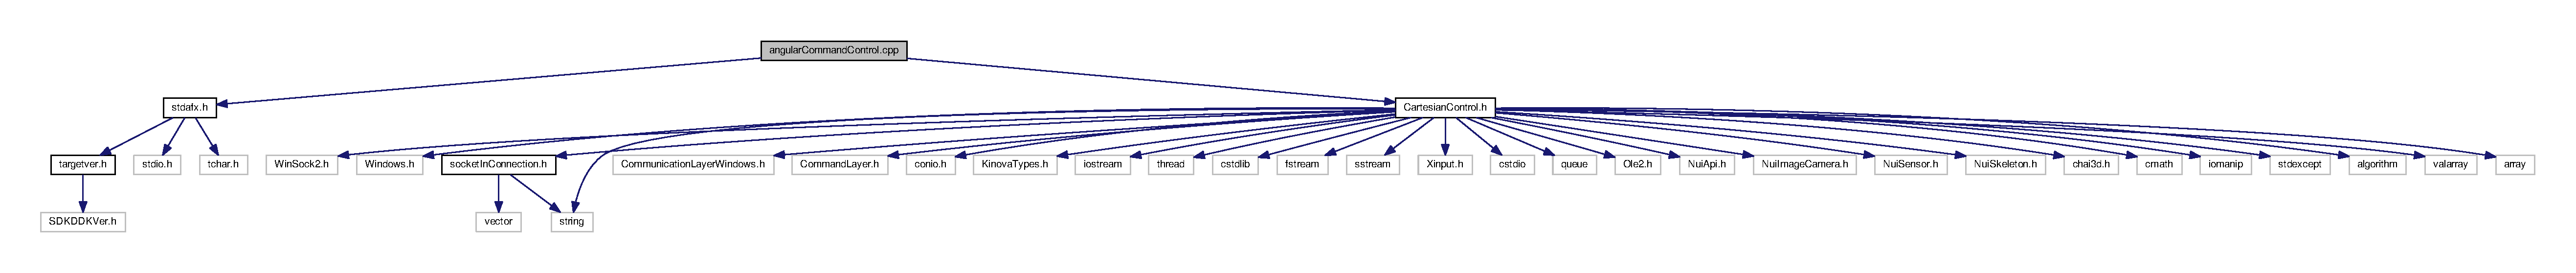
\includegraphics[width=350pt]{da/d87/angularCommandControl_8cpp__incl}
\end{center}
\end{figure}
\subsection*{Macros}
\begin{DoxyCompactItemize}
\item 
\#define \hyperlink{angularCommandControl_8cpp_adfc8f90f3a8caa8423099cf36ff214f1}{\+\_\+\+W\+I\+N\+S\+O\+C\+K\+\_\+\+D\+E\+P\+R\+E\+C\+A\+T\+E\+D\+\_\+\+N\+O\+\_\+\+W\+A\+R\+N\+I\+N\+GS}
\item 
\#define \hyperlink{angularCommandControl_8cpp_ac7bef5d85e3dcd73eef56ad39ffc84a9}{W\+I\+N32\+\_\+\+L\+E\+A\+N\+\_\+\+A\+N\+D\+\_\+\+M\+E\+AN}
\end{DoxyCompactItemize}


\subsection{Macro Definition Documentation}
\index{angular\+Command\+Control.\+cpp@{angular\+Command\+Control.\+cpp}!\+\_\+\+W\+I\+N\+S\+O\+C\+K\+\_\+\+D\+E\+P\+R\+E\+C\+A\+T\+E\+D\+\_\+\+N\+O\+\_\+\+W\+A\+R\+N\+I\+N\+GS@{\+\_\+\+W\+I\+N\+S\+O\+C\+K\+\_\+\+D\+E\+P\+R\+E\+C\+A\+T\+E\+D\+\_\+\+N\+O\+\_\+\+W\+A\+R\+N\+I\+N\+GS}}
\index{\+\_\+\+W\+I\+N\+S\+O\+C\+K\+\_\+\+D\+E\+P\+R\+E\+C\+A\+T\+E\+D\+\_\+\+N\+O\+\_\+\+W\+A\+R\+N\+I\+N\+GS@{\+\_\+\+W\+I\+N\+S\+O\+C\+K\+\_\+\+D\+E\+P\+R\+E\+C\+A\+T\+E\+D\+\_\+\+N\+O\+\_\+\+W\+A\+R\+N\+I\+N\+GS}!angular\+Command\+Control.\+cpp@{angular\+Command\+Control.\+cpp}}
\subsubsection[{\texorpdfstring{\+\_\+\+W\+I\+N\+S\+O\+C\+K\+\_\+\+D\+E\+P\+R\+E\+C\+A\+T\+E\+D\+\_\+\+N\+O\+\_\+\+W\+A\+R\+N\+I\+N\+GS}{_WINSOCK_DEPRECATED_NO_WARNINGS}}]{\setlength{\rightskip}{0pt plus 5cm}\#define \+\_\+\+W\+I\+N\+S\+O\+C\+K\+\_\+\+D\+E\+P\+R\+E\+C\+A\+T\+E\+D\+\_\+\+N\+O\+\_\+\+W\+A\+R\+N\+I\+N\+GS}\hypertarget{angularCommandControl_8cpp_adfc8f90f3a8caa8423099cf36ff214f1}{}\label{angularCommandControl_8cpp_adfc8f90f3a8caa8423099cf36ff214f1}
\index{angular\+Command\+Control.\+cpp@{angular\+Command\+Control.\+cpp}!W\+I\+N32\+\_\+\+L\+E\+A\+N\+\_\+\+A\+N\+D\+\_\+\+M\+E\+AN@{W\+I\+N32\+\_\+\+L\+E\+A\+N\+\_\+\+A\+N\+D\+\_\+\+M\+E\+AN}}
\index{W\+I\+N32\+\_\+\+L\+E\+A\+N\+\_\+\+A\+N\+D\+\_\+\+M\+E\+AN@{W\+I\+N32\+\_\+\+L\+E\+A\+N\+\_\+\+A\+N\+D\+\_\+\+M\+E\+AN}!angular\+Command\+Control.\+cpp@{angular\+Command\+Control.\+cpp}}
\subsubsection[{\texorpdfstring{W\+I\+N32\+\_\+\+L\+E\+A\+N\+\_\+\+A\+N\+D\+\_\+\+M\+E\+AN}{WIN32_LEAN_AND_MEAN}}]{\setlength{\rightskip}{0pt plus 5cm}\#define W\+I\+N32\+\_\+\+L\+E\+A\+N\+\_\+\+A\+N\+D\+\_\+\+M\+E\+AN}\hypertarget{angularCommandControl_8cpp_ac7bef5d85e3dcd73eef56ad39ffc84a9}{}\label{angularCommandControl_8cpp_ac7bef5d85e3dcd73eef56ad39ffc84a9}

\hypertarget{KinovaHMICartesianControl_2angularCommandControl_8cpp}{}\section{angular\+Command\+Control.\+cpp File Reference}
\label{KinovaHMICartesianControl_2angularCommandControl_8cpp}\index{angular\+Command\+Control.\+cpp@{angular\+Command\+Control.\+cpp}}
{\ttfamily \#include \char`\"{}stdafx.\+h\char`\"{}}\\*
{\ttfamily \#include \char`\"{}Cartesian\+Control.\+h\char`\"{}}\\*
Include dependency graph for Kinova\+H\+M\+I\+Cartesian\+Control/angular\+Command\+Control.cpp\+:
\nopagebreak
\begin{figure}[H]
\begin{center}
\leavevmode
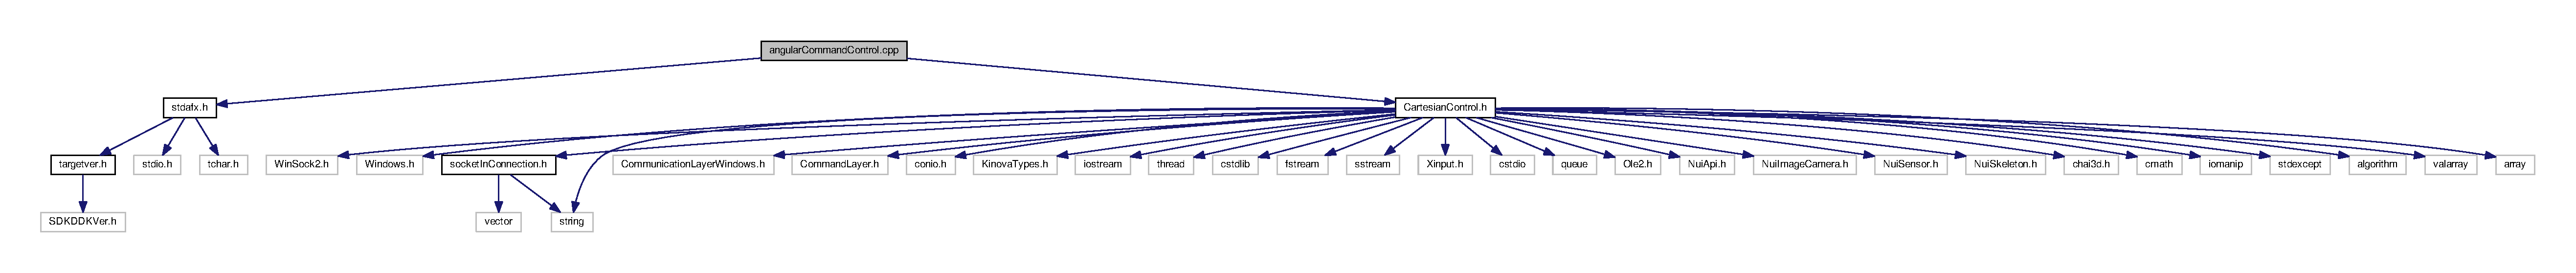
\includegraphics[width=350pt]{dc/dad/KinovaHMICartesianControl_2angularCommandControl_8cpp__incl}
\end{center}
\end{figure}
\subsection*{Macros}
\begin{DoxyCompactItemize}
\item 
\#define \hyperlink{KinovaHMICartesianControl_2angularCommandControl_8cpp_adfc8f90f3a8caa8423099cf36ff214f1}{\+\_\+\+W\+I\+N\+S\+O\+C\+K\+\_\+\+D\+E\+P\+R\+E\+C\+A\+T\+E\+D\+\_\+\+N\+O\+\_\+\+W\+A\+R\+N\+I\+N\+GS}
\item 
\#define \hyperlink{KinovaHMICartesianControl_2angularCommandControl_8cpp_ac7bef5d85e3dcd73eef56ad39ffc84a9}{W\+I\+N32\+\_\+\+L\+E\+A\+N\+\_\+\+A\+N\+D\+\_\+\+M\+E\+AN}
\end{DoxyCompactItemize}


\subsection{Macro Definition Documentation}
\index{Kinova\+H\+M\+I\+Cartesian\+Control/angular\+Command\+Control.\+cpp@{Kinova\+H\+M\+I\+Cartesian\+Control/angular\+Command\+Control.\+cpp}!\+\_\+\+W\+I\+N\+S\+O\+C\+K\+\_\+\+D\+E\+P\+R\+E\+C\+A\+T\+E\+D\+\_\+\+N\+O\+\_\+\+W\+A\+R\+N\+I\+N\+GS@{\+\_\+\+W\+I\+N\+S\+O\+C\+K\+\_\+\+D\+E\+P\+R\+E\+C\+A\+T\+E\+D\+\_\+\+N\+O\+\_\+\+W\+A\+R\+N\+I\+N\+GS}}
\index{\+\_\+\+W\+I\+N\+S\+O\+C\+K\+\_\+\+D\+E\+P\+R\+E\+C\+A\+T\+E\+D\+\_\+\+N\+O\+\_\+\+W\+A\+R\+N\+I\+N\+GS@{\+\_\+\+W\+I\+N\+S\+O\+C\+K\+\_\+\+D\+E\+P\+R\+E\+C\+A\+T\+E\+D\+\_\+\+N\+O\+\_\+\+W\+A\+R\+N\+I\+N\+GS}!Kinova\+H\+M\+I\+Cartesian\+Control/angular\+Command\+Control.\+cpp@{Kinova\+H\+M\+I\+Cartesian\+Control/angular\+Command\+Control.\+cpp}}
\subsubsection[{\texorpdfstring{\+\_\+\+W\+I\+N\+S\+O\+C\+K\+\_\+\+D\+E\+P\+R\+E\+C\+A\+T\+E\+D\+\_\+\+N\+O\+\_\+\+W\+A\+R\+N\+I\+N\+GS}{_WINSOCK_DEPRECATED_NO_WARNINGS}}]{\setlength{\rightskip}{0pt plus 5cm}\#define \+\_\+\+W\+I\+N\+S\+O\+C\+K\+\_\+\+D\+E\+P\+R\+E\+C\+A\+T\+E\+D\+\_\+\+N\+O\+\_\+\+W\+A\+R\+N\+I\+N\+GS}\hypertarget{KinovaHMICartesianControl_2angularCommandControl_8cpp_adfc8f90f3a8caa8423099cf36ff214f1}{}\label{KinovaHMICartesianControl_2angularCommandControl_8cpp_adfc8f90f3a8caa8423099cf36ff214f1}
\index{Kinova\+H\+M\+I\+Cartesian\+Control/angular\+Command\+Control.\+cpp@{Kinova\+H\+M\+I\+Cartesian\+Control/angular\+Command\+Control.\+cpp}!W\+I\+N32\+\_\+\+L\+E\+A\+N\+\_\+\+A\+N\+D\+\_\+\+M\+E\+AN@{W\+I\+N32\+\_\+\+L\+E\+A\+N\+\_\+\+A\+N\+D\+\_\+\+M\+E\+AN}}
\index{W\+I\+N32\+\_\+\+L\+E\+A\+N\+\_\+\+A\+N\+D\+\_\+\+M\+E\+AN@{W\+I\+N32\+\_\+\+L\+E\+A\+N\+\_\+\+A\+N\+D\+\_\+\+M\+E\+AN}!Kinova\+H\+M\+I\+Cartesian\+Control/angular\+Command\+Control.\+cpp@{Kinova\+H\+M\+I\+Cartesian\+Control/angular\+Command\+Control.\+cpp}}
\subsubsection[{\texorpdfstring{W\+I\+N32\+\_\+\+L\+E\+A\+N\+\_\+\+A\+N\+D\+\_\+\+M\+E\+AN}{WIN32_LEAN_AND_MEAN}}]{\setlength{\rightskip}{0pt plus 5cm}\#define W\+I\+N32\+\_\+\+L\+E\+A\+N\+\_\+\+A\+N\+D\+\_\+\+M\+E\+AN}\hypertarget{KinovaHMICartesianControl_2angularCommandControl_8cpp_ac7bef5d85e3dcd73eef56ad39ffc84a9}{}\label{KinovaHMICartesianControl_2angularCommandControl_8cpp_ac7bef5d85e3dcd73eef56ad39ffc84a9}

\hypertarget{CartesianControl_8h}{}\section{Cartesian\+Control.\+h File Reference}
\label{CartesianControl_8h}\index{Cartesian\+Control.\+h@{Cartesian\+Control.\+h}}
{\ttfamily \#include $<$Win\+Sock2.\+h$>$}\\*
{\ttfamily \#include $<$Windows.\+h$>$}\\*
{\ttfamily \#include \char`\"{}socket\+In\+Connection.\+h\char`\"{}}\\*
{\ttfamily \#include \char`\"{}Communication\+Layer\+Windows.\+h\char`\"{}}\\*
{\ttfamily \#include \char`\"{}Command\+Layer.\+h\char`\"{}}\\*
{\ttfamily \#include $<$conio.\+h$>$}\\*
{\ttfamily \#include \char`\"{}Kinova\+Types.\+h\char`\"{}}\\*
{\ttfamily \#include $<$iostream$>$}\\*
{\ttfamily \#include $<$thread$>$}\\*
{\ttfamily \#include $<$cstdlib$>$}\\*
{\ttfamily \#include $<$fstream$>$}\\*
{\ttfamily \#include $<$string$>$}\\*
{\ttfamily \#include $<$sstream$>$}\\*
{\ttfamily \#include $<$Xinput.\+h$>$}\\*
{\ttfamily \#include $<$cstdio$>$}\\*
{\ttfamily \#include $<$queue$>$}\\*
{\ttfamily \#include $<$Ole2.\+h$>$}\\*
{\ttfamily \#include \char`\"{}Nui\+Api.\+h\char`\"{}}\\*
{\ttfamily \#include \char`\"{}Nui\+Image\+Camera.\+h\char`\"{}}\\*
{\ttfamily \#include \char`\"{}Nui\+Sensor.\+h\char`\"{}}\\*
{\ttfamily \#include \char`\"{}Nui\+Skeleton.\+h\char`\"{}}\\*
{\ttfamily \#include \char`\"{}chai3d.\+h\char`\"{}}\\*
{\ttfamily \#include $<$cmath$>$}\\*
{\ttfamily \#include $<$iomanip$>$}\\*
{\ttfamily \#include $<$stdexcept$>$}\\*
{\ttfamily \#include $<$algorithm$>$}\\*
{\ttfamily \#include $<$valarray$>$}\\*
{\ttfamily \#include $<$array$>$}\\*
Include dependency graph for Cartesian\+Control.\+h\+:\nopagebreak
\begin{figure}[H]
\begin{center}
\leavevmode
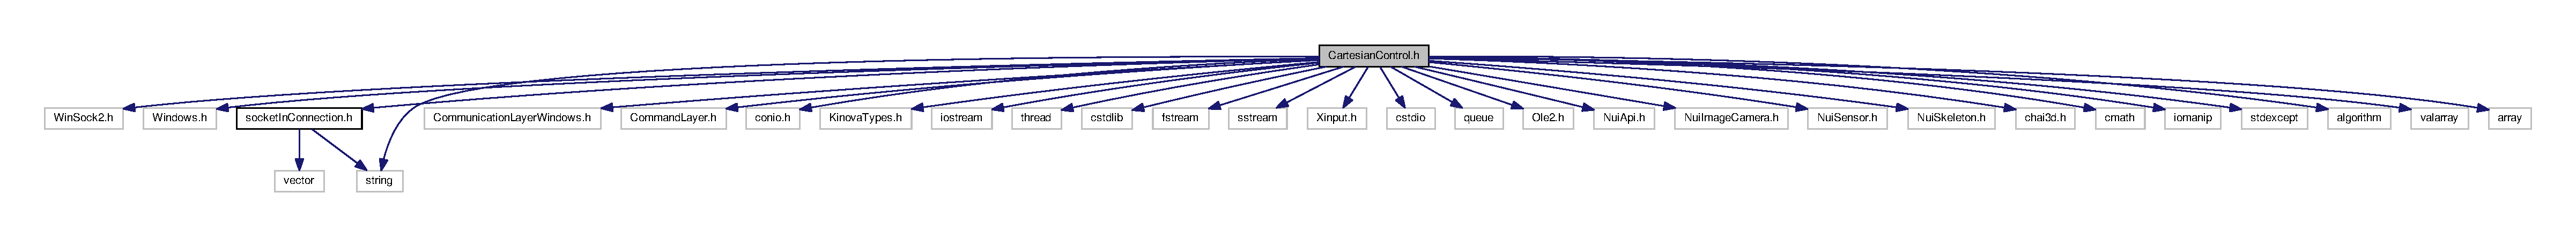
\includegraphics[width=350pt]{d0/d3f/CartesianControl_8h__incl}
\end{center}
\end{figure}
This graph shows which files directly or indirectly include this file\+:\nopagebreak
\begin{figure}[H]
\begin{center}
\leavevmode
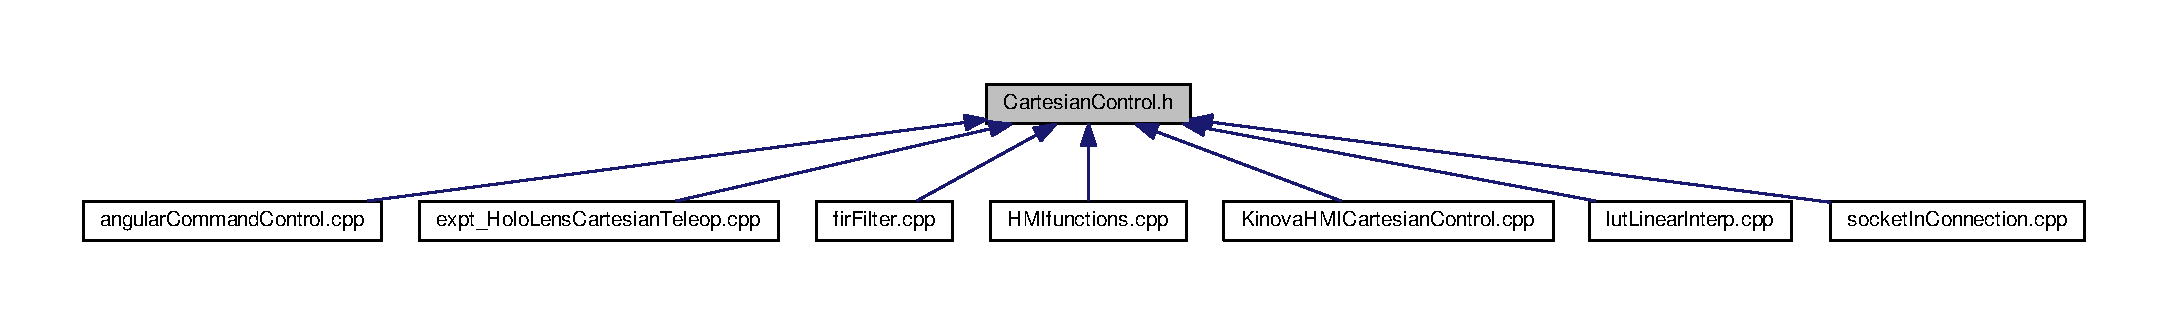
\includegraphics[width=350pt]{d3/d8d/CartesianControl_8h__dep__incl}
\end{center}
\end{figure}
\subsection*{Classes}
\begin{DoxyCompactItemize}
\item 
class \hyperlink{classCXBOXController}{C\+X\+B\+O\+X\+Controller}
\item 
class \hyperlink{classTimer}{Timer}
\item 
class \hyperlink{classKinovaAPIFunctions}{Kinova\+A\+P\+I\+Functions}
\item 
class \hyperlink{classkinectSkelTrack}{kinect\+Skel\+Track}
\item 
struct \hyperlink{structkinectSkelTrack_1_1KinectInfo}{kinect\+Skel\+Track\+::\+Kinect\+Info}
\item 
class \hyperlink{classFIRFilter}{F\+I\+R\+Filter}
\item 
class \hyperlink{classExperiment}{Experiment}
\item 
class \hyperlink{classNovintFalconHapticsDevice}{Novint\+Falcon\+Haptics\+Device}
\end{DoxyCompactItemize}
\subsection*{Macros}
\begin{DoxyCompactItemize}
\item 
\#define \hyperlink{CartesianControl_8h_adfc8f90f3a8caa8423099cf36ff214f1}{\+\_\+\+W\+I\+N\+S\+O\+C\+K\+\_\+\+D\+E\+P\+R\+E\+C\+A\+T\+E\+D\+\_\+\+N\+O\+\_\+\+W\+A\+R\+N\+I\+N\+GS}
\item 
\#define \hyperlink{CartesianControl_8h_ac7bef5d85e3dcd73eef56ad39ffc84a9}{W\+I\+N32\+\_\+\+L\+E\+A\+N\+\_\+\+A\+N\+D\+\_\+\+M\+E\+AN}
\item 
\#define \hyperlink{CartesianControl_8h_ac7bef5d85e3dcd73eef56ad39ffc84a9}{W\+I\+N32\+\_\+\+L\+E\+A\+N\+\_\+\+A\+N\+D\+\_\+\+M\+E\+AN}
\item 
\#define \hyperlink{CartesianControl_8h_a0934169ae417a287adfd19bdd7a13137}{U\+S\+E\+\_\+\+K\+I\+N\+O\+VA}~true
\item 
\#define \hyperlink{CartesianControl_8h_a4b87829c8dfd2ba03fdc55f059b87bef}{U\+S\+E\+\_\+\+K\+I\+N\+E\+CT}~false
\item 
\#define \hyperlink{CartesianControl_8h_a1a02ac5217ce78990cacecfae4f6d509}{U\+S\+E\+\_\+\+T\+CP}~true
\item 
\#define \hyperlink{CartesianControl_8h_ad15cf97d77a6dd54ab0e2c90387bcb0b}{U\+S\+E\+\_\+\+H\+A\+P\+T\+I\+CS}~true
\item 
\#define \hyperlink{CartesianControl_8h_aec53ee0acd16d9f951bc2f63235fa914}{G\+N\+U\+P\+L\+OT}~false
\item 
\#define \hyperlink{CartesianControl_8h_a889394d13af6d709e557cdc4a16db344}{\+\_\+\+X\+B\+O\+X\+\_\+\+C\+O\+N\+T\+R\+O\+L\+L\+E\+R\+\_\+\+H\+\_\+}
\item 
\#define \hyperlink{CartesianControl_8h_ac7bef5d85e3dcd73eef56ad39ffc84a9}{W\+I\+N32\+\_\+\+L\+E\+A\+N\+\_\+\+A\+N\+D\+\_\+\+M\+E\+AN}
\item 
\#define \hyperlink{CartesianControl_8h_a46130dc86f2322714bba26960b64e7bb}{B\+U\+F\+F\+E\+R\+\_\+\+L\+EN}~96
\begin{DoxyCompactList}\small\item\em Buffer length to hold input samples of F\+IR Filter. \end{DoxyCompactList}\end{DoxyCompactItemize}


\subsection{Macro Definition Documentation}
\index{Cartesian\+Control.\+h@{Cartesian\+Control.\+h}!\+\_\+\+W\+I\+N\+S\+O\+C\+K\+\_\+\+D\+E\+P\+R\+E\+C\+A\+T\+E\+D\+\_\+\+N\+O\+\_\+\+W\+A\+R\+N\+I\+N\+GS@{\+\_\+\+W\+I\+N\+S\+O\+C\+K\+\_\+\+D\+E\+P\+R\+E\+C\+A\+T\+E\+D\+\_\+\+N\+O\+\_\+\+W\+A\+R\+N\+I\+N\+GS}}
\index{\+\_\+\+W\+I\+N\+S\+O\+C\+K\+\_\+\+D\+E\+P\+R\+E\+C\+A\+T\+E\+D\+\_\+\+N\+O\+\_\+\+W\+A\+R\+N\+I\+N\+GS@{\+\_\+\+W\+I\+N\+S\+O\+C\+K\+\_\+\+D\+E\+P\+R\+E\+C\+A\+T\+E\+D\+\_\+\+N\+O\+\_\+\+W\+A\+R\+N\+I\+N\+GS}!Cartesian\+Control.\+h@{Cartesian\+Control.\+h}}
\subsubsection[{\texorpdfstring{\+\_\+\+W\+I\+N\+S\+O\+C\+K\+\_\+\+D\+E\+P\+R\+E\+C\+A\+T\+E\+D\+\_\+\+N\+O\+\_\+\+W\+A\+R\+N\+I\+N\+GS}{_WINSOCK_DEPRECATED_NO_WARNINGS}}]{\setlength{\rightskip}{0pt plus 5cm}\#define \+\_\+\+W\+I\+N\+S\+O\+C\+K\+\_\+\+D\+E\+P\+R\+E\+C\+A\+T\+E\+D\+\_\+\+N\+O\+\_\+\+W\+A\+R\+N\+I\+N\+GS}\hypertarget{CartesianControl_8h_adfc8f90f3a8caa8423099cf36ff214f1}{}\label{CartesianControl_8h_adfc8f90f3a8caa8423099cf36ff214f1}
\index{Cartesian\+Control.\+h@{Cartesian\+Control.\+h}!\+\_\+\+X\+B\+O\+X\+\_\+\+C\+O\+N\+T\+R\+O\+L\+L\+E\+R\+\_\+\+H\+\_\+@{\+\_\+\+X\+B\+O\+X\+\_\+\+C\+O\+N\+T\+R\+O\+L\+L\+E\+R\+\_\+\+H\+\_\+}}
\index{\+\_\+\+X\+B\+O\+X\+\_\+\+C\+O\+N\+T\+R\+O\+L\+L\+E\+R\+\_\+\+H\+\_\+@{\+\_\+\+X\+B\+O\+X\+\_\+\+C\+O\+N\+T\+R\+O\+L\+L\+E\+R\+\_\+\+H\+\_\+}!Cartesian\+Control.\+h@{Cartesian\+Control.\+h}}
\subsubsection[{\texorpdfstring{\+\_\+\+X\+B\+O\+X\+\_\+\+C\+O\+N\+T\+R\+O\+L\+L\+E\+R\+\_\+\+H\+\_\+}{_XBOX_CONTROLLER_H_}}]{\setlength{\rightskip}{0pt plus 5cm}\#define \+\_\+\+X\+B\+O\+X\+\_\+\+C\+O\+N\+T\+R\+O\+L\+L\+E\+R\+\_\+\+H\+\_\+}\hypertarget{CartesianControl_8h_a889394d13af6d709e557cdc4a16db344}{}\label{CartesianControl_8h_a889394d13af6d709e557cdc4a16db344}
\index{Cartesian\+Control.\+h@{Cartesian\+Control.\+h}!B\+U\+F\+F\+E\+R\+\_\+\+L\+EN@{B\+U\+F\+F\+E\+R\+\_\+\+L\+EN}}
\index{B\+U\+F\+F\+E\+R\+\_\+\+L\+EN@{B\+U\+F\+F\+E\+R\+\_\+\+L\+EN}!Cartesian\+Control.\+h@{Cartesian\+Control.\+h}}
\subsubsection[{\texorpdfstring{B\+U\+F\+F\+E\+R\+\_\+\+L\+EN}{BUFFER_LEN}}]{\setlength{\rightskip}{0pt plus 5cm}\#define B\+U\+F\+F\+E\+R\+\_\+\+L\+EN~96}\hypertarget{CartesianControl_8h_a46130dc86f2322714bba26960b64e7bb}{}\label{CartesianControl_8h_a46130dc86f2322714bba26960b64e7bb}


Buffer length to hold input samples of F\+IR Filter. 

\index{Cartesian\+Control.\+h@{Cartesian\+Control.\+h}!G\+N\+U\+P\+L\+OT@{G\+N\+U\+P\+L\+OT}}
\index{G\+N\+U\+P\+L\+OT@{G\+N\+U\+P\+L\+OT}!Cartesian\+Control.\+h@{Cartesian\+Control.\+h}}
\subsubsection[{\texorpdfstring{G\+N\+U\+P\+L\+OT}{GNUPLOT}}]{\setlength{\rightskip}{0pt plus 5cm}\#define G\+N\+U\+P\+L\+OT~false}\hypertarget{CartesianControl_8h_aec53ee0acd16d9f951bc2f63235fa914}{}\label{CartesianControl_8h_aec53ee0acd16d9f951bc2f63235fa914}
\index{Cartesian\+Control.\+h@{Cartesian\+Control.\+h}!U\+S\+E\+\_\+\+H\+A\+P\+T\+I\+CS@{U\+S\+E\+\_\+\+H\+A\+P\+T\+I\+CS}}
\index{U\+S\+E\+\_\+\+H\+A\+P\+T\+I\+CS@{U\+S\+E\+\_\+\+H\+A\+P\+T\+I\+CS}!Cartesian\+Control.\+h@{Cartesian\+Control.\+h}}
\subsubsection[{\texorpdfstring{U\+S\+E\+\_\+\+H\+A\+P\+T\+I\+CS}{USE_HAPTICS}}]{\setlength{\rightskip}{0pt plus 5cm}\#define U\+S\+E\+\_\+\+H\+A\+P\+T\+I\+CS~true}\hypertarget{CartesianControl_8h_ad15cf97d77a6dd54ab0e2c90387bcb0b}{}\label{CartesianControl_8h_ad15cf97d77a6dd54ab0e2c90387bcb0b}
\index{Cartesian\+Control.\+h@{Cartesian\+Control.\+h}!U\+S\+E\+\_\+\+K\+I\+N\+E\+CT@{U\+S\+E\+\_\+\+K\+I\+N\+E\+CT}}
\index{U\+S\+E\+\_\+\+K\+I\+N\+E\+CT@{U\+S\+E\+\_\+\+K\+I\+N\+E\+CT}!Cartesian\+Control.\+h@{Cartesian\+Control.\+h}}
\subsubsection[{\texorpdfstring{U\+S\+E\+\_\+\+K\+I\+N\+E\+CT}{USE_KINECT}}]{\setlength{\rightskip}{0pt plus 5cm}\#define U\+S\+E\+\_\+\+K\+I\+N\+E\+CT~false}\hypertarget{CartesianControl_8h_a4b87829c8dfd2ba03fdc55f059b87bef}{}\label{CartesianControl_8h_a4b87829c8dfd2ba03fdc55f059b87bef}
\index{Cartesian\+Control.\+h@{Cartesian\+Control.\+h}!U\+S\+E\+\_\+\+K\+I\+N\+O\+VA@{U\+S\+E\+\_\+\+K\+I\+N\+O\+VA}}
\index{U\+S\+E\+\_\+\+K\+I\+N\+O\+VA@{U\+S\+E\+\_\+\+K\+I\+N\+O\+VA}!Cartesian\+Control.\+h@{Cartesian\+Control.\+h}}
\subsubsection[{\texorpdfstring{U\+S\+E\+\_\+\+K\+I\+N\+O\+VA}{USE_KINOVA}}]{\setlength{\rightskip}{0pt plus 5cm}\#define U\+S\+E\+\_\+\+K\+I\+N\+O\+VA~true}\hypertarget{CartesianControl_8h_a0934169ae417a287adfd19bdd7a13137}{}\label{CartesianControl_8h_a0934169ae417a287adfd19bdd7a13137}
\index{Cartesian\+Control.\+h@{Cartesian\+Control.\+h}!U\+S\+E\+\_\+\+T\+CP@{U\+S\+E\+\_\+\+T\+CP}}
\index{U\+S\+E\+\_\+\+T\+CP@{U\+S\+E\+\_\+\+T\+CP}!Cartesian\+Control.\+h@{Cartesian\+Control.\+h}}
\subsubsection[{\texorpdfstring{U\+S\+E\+\_\+\+T\+CP}{USE_TCP}}]{\setlength{\rightskip}{0pt plus 5cm}\#define U\+S\+E\+\_\+\+T\+CP~true}\hypertarget{CartesianControl_8h_a1a02ac5217ce78990cacecfae4f6d509}{}\label{CartesianControl_8h_a1a02ac5217ce78990cacecfae4f6d509}
\index{Cartesian\+Control.\+h@{Cartesian\+Control.\+h}!W\+I\+N32\+\_\+\+L\+E\+A\+N\+\_\+\+A\+N\+D\+\_\+\+M\+E\+AN@{W\+I\+N32\+\_\+\+L\+E\+A\+N\+\_\+\+A\+N\+D\+\_\+\+M\+E\+AN}}
\index{W\+I\+N32\+\_\+\+L\+E\+A\+N\+\_\+\+A\+N\+D\+\_\+\+M\+E\+AN@{W\+I\+N32\+\_\+\+L\+E\+A\+N\+\_\+\+A\+N\+D\+\_\+\+M\+E\+AN}!Cartesian\+Control.\+h@{Cartesian\+Control.\+h}}
\subsubsection[{\texorpdfstring{W\+I\+N32\+\_\+\+L\+E\+A\+N\+\_\+\+A\+N\+D\+\_\+\+M\+E\+AN}{WIN32_LEAN_AND_MEAN}}]{\setlength{\rightskip}{0pt plus 5cm}\#define W\+I\+N32\+\_\+\+L\+E\+A\+N\+\_\+\+A\+N\+D\+\_\+\+M\+E\+AN}\hypertarget{CartesianControl_8h_ac7bef5d85e3dcd73eef56ad39ffc84a9}{}\label{CartesianControl_8h_ac7bef5d85e3dcd73eef56ad39ffc84a9}
\index{Cartesian\+Control.\+h@{Cartesian\+Control.\+h}!W\+I\+N32\+\_\+\+L\+E\+A\+N\+\_\+\+A\+N\+D\+\_\+\+M\+E\+AN@{W\+I\+N32\+\_\+\+L\+E\+A\+N\+\_\+\+A\+N\+D\+\_\+\+M\+E\+AN}}
\index{W\+I\+N32\+\_\+\+L\+E\+A\+N\+\_\+\+A\+N\+D\+\_\+\+M\+E\+AN@{W\+I\+N32\+\_\+\+L\+E\+A\+N\+\_\+\+A\+N\+D\+\_\+\+M\+E\+AN}!Cartesian\+Control.\+h@{Cartesian\+Control.\+h}}
\subsubsection[{\texorpdfstring{W\+I\+N32\+\_\+\+L\+E\+A\+N\+\_\+\+A\+N\+D\+\_\+\+M\+E\+AN}{WIN32_LEAN_AND_MEAN}}]{\setlength{\rightskip}{0pt plus 5cm}\#define W\+I\+N32\+\_\+\+L\+E\+A\+N\+\_\+\+A\+N\+D\+\_\+\+M\+E\+AN}\hypertarget{CartesianControl_8h_ac7bef5d85e3dcd73eef56ad39ffc84a9}{}\label{CartesianControl_8h_ac7bef5d85e3dcd73eef56ad39ffc84a9}
\index{Cartesian\+Control.\+h@{Cartesian\+Control.\+h}!W\+I\+N32\+\_\+\+L\+E\+A\+N\+\_\+\+A\+N\+D\+\_\+\+M\+E\+AN@{W\+I\+N32\+\_\+\+L\+E\+A\+N\+\_\+\+A\+N\+D\+\_\+\+M\+E\+AN}}
\index{W\+I\+N32\+\_\+\+L\+E\+A\+N\+\_\+\+A\+N\+D\+\_\+\+M\+E\+AN@{W\+I\+N32\+\_\+\+L\+E\+A\+N\+\_\+\+A\+N\+D\+\_\+\+M\+E\+AN}!Cartesian\+Control.\+h@{Cartesian\+Control.\+h}}
\subsubsection[{\texorpdfstring{W\+I\+N32\+\_\+\+L\+E\+A\+N\+\_\+\+A\+N\+D\+\_\+\+M\+E\+AN}{WIN32_LEAN_AND_MEAN}}]{\setlength{\rightskip}{0pt plus 5cm}\#define W\+I\+N32\+\_\+\+L\+E\+A\+N\+\_\+\+A\+N\+D\+\_\+\+M\+E\+AN}\hypertarget{CartesianControl_8h_ac7bef5d85e3dcd73eef56ad39ffc84a9}{}\label{CartesianControl_8h_ac7bef5d85e3dcd73eef56ad39ffc84a9}

\hypertarget{KinovaHMICartesianControl_2CartesianControl_8h}{}\section{Cartesian\+Control.\+h File Reference}
\label{KinovaHMICartesianControl_2CartesianControl_8h}\index{Cartesian\+Control.\+h@{Cartesian\+Control.\+h}}
{\ttfamily \#include $<$Win\+Sock2.\+h$>$}\\*
{\ttfamily \#include $<$Windows.\+h$>$}\\*
{\ttfamily \#include \char`\"{}socket\+In\+Connection.\+h\char`\"{}}\\*
{\ttfamily \#include \char`\"{}Communication\+Layer\+Windows.\+h\char`\"{}}\\*
{\ttfamily \#include \char`\"{}Command\+Layer.\+h\char`\"{}}\\*
{\ttfamily \#include $<$conio.\+h$>$}\\*
{\ttfamily \#include \char`\"{}Kinova\+Types.\+h\char`\"{}}\\*
{\ttfamily \#include $<$iostream$>$}\\*
{\ttfamily \#include $<$thread$>$}\\*
{\ttfamily \#include $<$cstdlib$>$}\\*
{\ttfamily \#include $<$fstream$>$}\\*
{\ttfamily \#include $<$string$>$}\\*
{\ttfamily \#include $<$sstream$>$}\\*
{\ttfamily \#include $<$Xinput.\+h$>$}\\*
{\ttfamily \#include $<$cstdio$>$}\\*
{\ttfamily \#include $<$queue$>$}\\*
{\ttfamily \#include $<$Ole2.\+h$>$}\\*
{\ttfamily \#include \char`\"{}Nui\+Api.\+h\char`\"{}}\\*
{\ttfamily \#include \char`\"{}Nui\+Image\+Camera.\+h\char`\"{}}\\*
{\ttfamily \#include \char`\"{}Nui\+Sensor.\+h\char`\"{}}\\*
{\ttfamily \#include \char`\"{}Nui\+Skeleton.\+h\char`\"{}}\\*
{\ttfamily \#include \char`\"{}chai3d.\+h\char`\"{}}\\*
{\ttfamily \#include $<$cmath$>$}\\*
{\ttfamily \#include $<$iomanip$>$}\\*
{\ttfamily \#include $<$stdexcept$>$}\\*
{\ttfamily \#include $<$algorithm$>$}\\*
{\ttfamily \#include $<$valarray$>$}\\*
{\ttfamily \#include $<$array$>$}\\*
Include dependency graph for Kinova\+H\+M\+I\+Cartesian\+Control/\+Cartesian\+Control.h\+:
\nopagebreak
\begin{figure}[H]
\begin{center}
\leavevmode
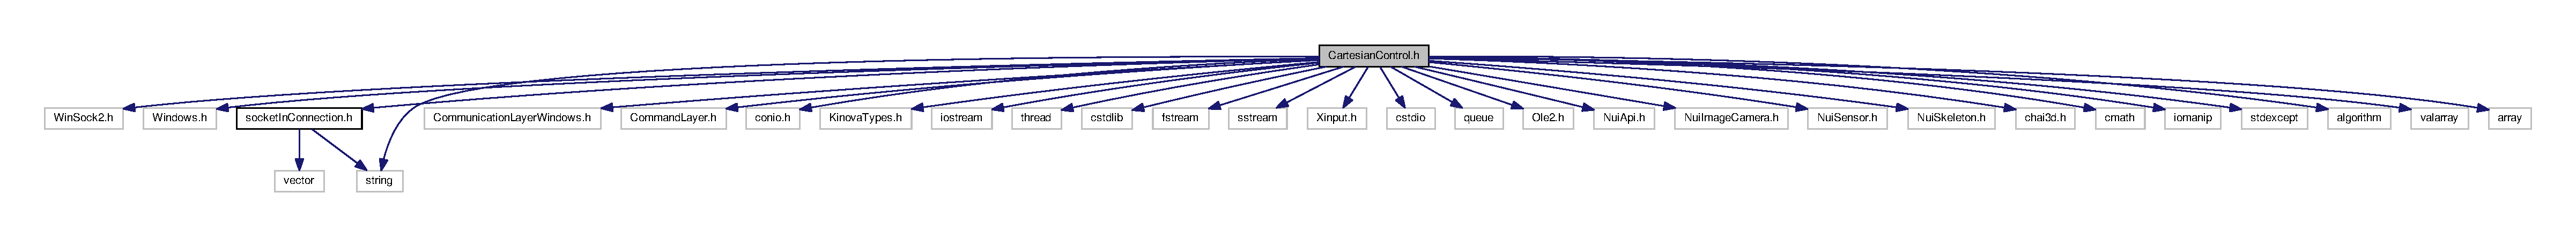
\includegraphics[width=350pt]{d4/db2/KinovaHMICartesianControl_2CartesianControl_8h__incl}
\end{center}
\end{figure}
This graph shows which files directly or indirectly include this file\+:
\nopagebreak
\begin{figure}[H]
\begin{center}
\leavevmode
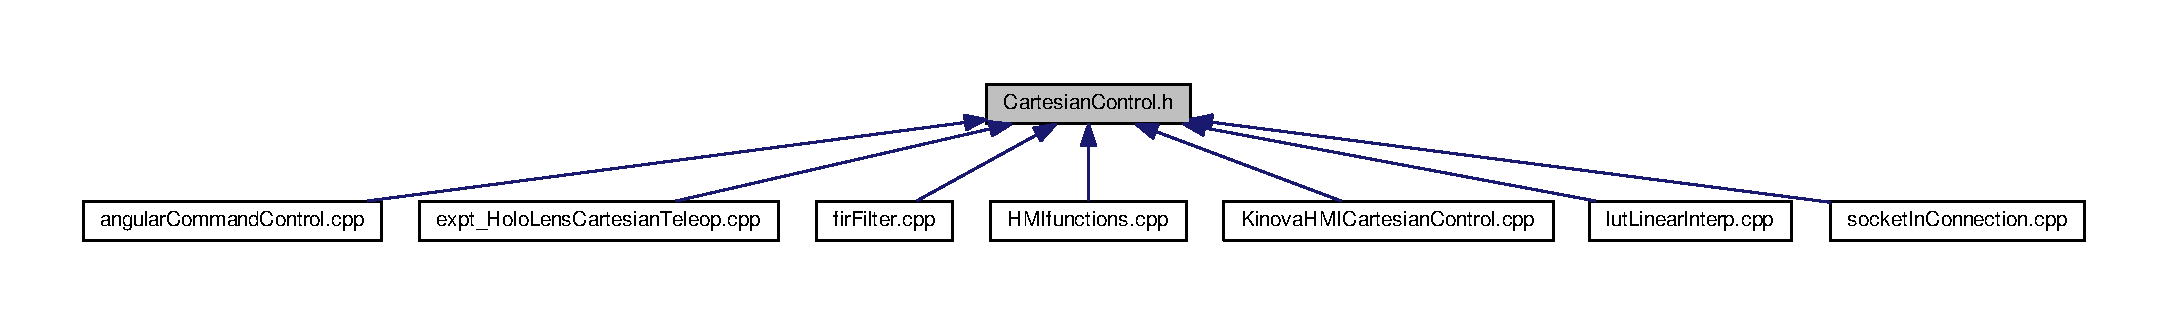
\includegraphics[width=350pt]{df/daf/KinovaHMICartesianControl_2CartesianControl_8h__dep__incl}
\end{center}
\end{figure}
\subsection*{Classes}
\begin{DoxyCompactItemize}
\item 
class \hyperlink{classCXBOXController}{C\+X\+B\+O\+X\+Controller}
\item 
class \hyperlink{classTimer}{Timer}
\item 
class \hyperlink{classKinovaAPIFunctions}{Kinova\+A\+P\+I\+Functions}
\item 
class \hyperlink{classkinectSkelTrack}{kinect\+Skel\+Track}
\item 
struct \hyperlink{structkinectSkelTrack_1_1KinectInfo}{kinect\+Skel\+Track\+::\+Kinect\+Info}
\item 
class \hyperlink{classFIRFilter}{F\+I\+R\+Filter}
\item 
class \hyperlink{classExperiment}{Experiment}
\item 
class \hyperlink{classNovintFalconHapticsDevice}{Novint\+Falcon\+Haptics\+Device}
\end{DoxyCompactItemize}
\subsection*{Macros}
\begin{DoxyCompactItemize}
\item 
\#define \hyperlink{KinovaHMICartesianControl_2CartesianControl_8h_adfc8f90f3a8caa8423099cf36ff214f1}{\+\_\+\+W\+I\+N\+S\+O\+C\+K\+\_\+\+D\+E\+P\+R\+E\+C\+A\+T\+E\+D\+\_\+\+N\+O\+\_\+\+W\+A\+R\+N\+I\+N\+GS}
\item 
\#define \hyperlink{KinovaHMICartesianControl_2CartesianControl_8h_ac7bef5d85e3dcd73eef56ad39ffc84a9}{W\+I\+N32\+\_\+\+L\+E\+A\+N\+\_\+\+A\+N\+D\+\_\+\+M\+E\+AN}
\item 
\#define \hyperlink{KinovaHMICartesianControl_2CartesianControl_8h_ac7bef5d85e3dcd73eef56ad39ffc84a9}{W\+I\+N32\+\_\+\+L\+E\+A\+N\+\_\+\+A\+N\+D\+\_\+\+M\+E\+AN}
\item 
\#define \hyperlink{KinovaHMICartesianControl_2CartesianControl_8h_a0934169ae417a287adfd19bdd7a13137}{U\+S\+E\+\_\+\+K\+I\+N\+O\+VA}~true
\item 
\#define \hyperlink{KinovaHMICartesianControl_2CartesianControl_8h_a4b87829c8dfd2ba03fdc55f059b87bef}{U\+S\+E\+\_\+\+K\+I\+N\+E\+CT}~false
\item 
\#define \hyperlink{KinovaHMICartesianControl_2CartesianControl_8h_a1a02ac5217ce78990cacecfae4f6d509}{U\+S\+E\+\_\+\+T\+CP}~true
\item 
\#define \hyperlink{KinovaHMICartesianControl_2CartesianControl_8h_ad15cf97d77a6dd54ab0e2c90387bcb0b}{U\+S\+E\+\_\+\+H\+A\+P\+T\+I\+CS}~true
\item 
\#define \hyperlink{KinovaHMICartesianControl_2CartesianControl_8h_aec53ee0acd16d9f951bc2f63235fa914}{G\+N\+U\+P\+L\+OT}~false
\item 
\#define \hyperlink{KinovaHMICartesianControl_2CartesianControl_8h_a889394d13af6d709e557cdc4a16db344}{\+\_\+\+X\+B\+O\+X\+\_\+\+C\+O\+N\+T\+R\+O\+L\+L\+E\+R\+\_\+\+H\+\_\+}
\item 
\#define \hyperlink{KinovaHMICartesianControl_2CartesianControl_8h_ac7bef5d85e3dcd73eef56ad39ffc84a9}{W\+I\+N32\+\_\+\+L\+E\+A\+N\+\_\+\+A\+N\+D\+\_\+\+M\+E\+AN}
\item 
\#define \hyperlink{KinovaHMICartesianControl_2CartesianControl_8h_a46130dc86f2322714bba26960b64e7bb}{B\+U\+F\+F\+E\+R\+\_\+\+L\+EN}~96
\begin{DoxyCompactList}\small\item\em Buffer length to hold input samples of F\+IR Filter. \end{DoxyCompactList}\end{DoxyCompactItemize}


\subsection{Macro Definition Documentation}
\index{Kinova\+H\+M\+I\+Cartesian\+Control/\+Cartesian\+Control.\+h@{Kinova\+H\+M\+I\+Cartesian\+Control/\+Cartesian\+Control.\+h}!\+\_\+\+W\+I\+N\+S\+O\+C\+K\+\_\+\+D\+E\+P\+R\+E\+C\+A\+T\+E\+D\+\_\+\+N\+O\+\_\+\+W\+A\+R\+N\+I\+N\+GS@{\+\_\+\+W\+I\+N\+S\+O\+C\+K\+\_\+\+D\+E\+P\+R\+E\+C\+A\+T\+E\+D\+\_\+\+N\+O\+\_\+\+W\+A\+R\+N\+I\+N\+GS}}
\index{\+\_\+\+W\+I\+N\+S\+O\+C\+K\+\_\+\+D\+E\+P\+R\+E\+C\+A\+T\+E\+D\+\_\+\+N\+O\+\_\+\+W\+A\+R\+N\+I\+N\+GS@{\+\_\+\+W\+I\+N\+S\+O\+C\+K\+\_\+\+D\+E\+P\+R\+E\+C\+A\+T\+E\+D\+\_\+\+N\+O\+\_\+\+W\+A\+R\+N\+I\+N\+GS}!Kinova\+H\+M\+I\+Cartesian\+Control/\+Cartesian\+Control.\+h@{Kinova\+H\+M\+I\+Cartesian\+Control/\+Cartesian\+Control.\+h}}
\subsubsection[{\texorpdfstring{\+\_\+\+W\+I\+N\+S\+O\+C\+K\+\_\+\+D\+E\+P\+R\+E\+C\+A\+T\+E\+D\+\_\+\+N\+O\+\_\+\+W\+A\+R\+N\+I\+N\+GS}{_WINSOCK_DEPRECATED_NO_WARNINGS}}]{\setlength{\rightskip}{0pt plus 5cm}\#define \+\_\+\+W\+I\+N\+S\+O\+C\+K\+\_\+\+D\+E\+P\+R\+E\+C\+A\+T\+E\+D\+\_\+\+N\+O\+\_\+\+W\+A\+R\+N\+I\+N\+GS}\hypertarget{KinovaHMICartesianControl_2CartesianControl_8h_adfc8f90f3a8caa8423099cf36ff214f1}{}\label{KinovaHMICartesianControl_2CartesianControl_8h_adfc8f90f3a8caa8423099cf36ff214f1}
\index{Kinova\+H\+M\+I\+Cartesian\+Control/\+Cartesian\+Control.\+h@{Kinova\+H\+M\+I\+Cartesian\+Control/\+Cartesian\+Control.\+h}!\+\_\+\+X\+B\+O\+X\+\_\+\+C\+O\+N\+T\+R\+O\+L\+L\+E\+R\+\_\+\+H\+\_\+@{\+\_\+\+X\+B\+O\+X\+\_\+\+C\+O\+N\+T\+R\+O\+L\+L\+E\+R\+\_\+\+H\+\_\+}}
\index{\+\_\+\+X\+B\+O\+X\+\_\+\+C\+O\+N\+T\+R\+O\+L\+L\+E\+R\+\_\+\+H\+\_\+@{\+\_\+\+X\+B\+O\+X\+\_\+\+C\+O\+N\+T\+R\+O\+L\+L\+E\+R\+\_\+\+H\+\_\+}!Kinova\+H\+M\+I\+Cartesian\+Control/\+Cartesian\+Control.\+h@{Kinova\+H\+M\+I\+Cartesian\+Control/\+Cartesian\+Control.\+h}}
\subsubsection[{\texorpdfstring{\+\_\+\+X\+B\+O\+X\+\_\+\+C\+O\+N\+T\+R\+O\+L\+L\+E\+R\+\_\+\+H\+\_\+}{_XBOX_CONTROLLER_H_}}]{\setlength{\rightskip}{0pt plus 5cm}\#define \+\_\+\+X\+B\+O\+X\+\_\+\+C\+O\+N\+T\+R\+O\+L\+L\+E\+R\+\_\+\+H\+\_\+}\hypertarget{KinovaHMICartesianControl_2CartesianControl_8h_a889394d13af6d709e557cdc4a16db344}{}\label{KinovaHMICartesianControl_2CartesianControl_8h_a889394d13af6d709e557cdc4a16db344}
\index{Kinova\+H\+M\+I\+Cartesian\+Control/\+Cartesian\+Control.\+h@{Kinova\+H\+M\+I\+Cartesian\+Control/\+Cartesian\+Control.\+h}!B\+U\+F\+F\+E\+R\+\_\+\+L\+EN@{B\+U\+F\+F\+E\+R\+\_\+\+L\+EN}}
\index{B\+U\+F\+F\+E\+R\+\_\+\+L\+EN@{B\+U\+F\+F\+E\+R\+\_\+\+L\+EN}!Kinova\+H\+M\+I\+Cartesian\+Control/\+Cartesian\+Control.\+h@{Kinova\+H\+M\+I\+Cartesian\+Control/\+Cartesian\+Control.\+h}}
\subsubsection[{\texorpdfstring{B\+U\+F\+F\+E\+R\+\_\+\+L\+EN}{BUFFER_LEN}}]{\setlength{\rightskip}{0pt plus 5cm}\#define B\+U\+F\+F\+E\+R\+\_\+\+L\+EN~96}\hypertarget{KinovaHMICartesianControl_2CartesianControl_8h_a46130dc86f2322714bba26960b64e7bb}{}\label{KinovaHMICartesianControl_2CartesianControl_8h_a46130dc86f2322714bba26960b64e7bb}


Buffer length to hold input samples of F\+IR Filter. 

\index{Kinova\+H\+M\+I\+Cartesian\+Control/\+Cartesian\+Control.\+h@{Kinova\+H\+M\+I\+Cartesian\+Control/\+Cartesian\+Control.\+h}!G\+N\+U\+P\+L\+OT@{G\+N\+U\+P\+L\+OT}}
\index{G\+N\+U\+P\+L\+OT@{G\+N\+U\+P\+L\+OT}!Kinova\+H\+M\+I\+Cartesian\+Control/\+Cartesian\+Control.\+h@{Kinova\+H\+M\+I\+Cartesian\+Control/\+Cartesian\+Control.\+h}}
\subsubsection[{\texorpdfstring{G\+N\+U\+P\+L\+OT}{GNUPLOT}}]{\setlength{\rightskip}{0pt plus 5cm}\#define G\+N\+U\+P\+L\+OT~false}\hypertarget{KinovaHMICartesianControl_2CartesianControl_8h_aec53ee0acd16d9f951bc2f63235fa914}{}\label{KinovaHMICartesianControl_2CartesianControl_8h_aec53ee0acd16d9f951bc2f63235fa914}
\index{Kinova\+H\+M\+I\+Cartesian\+Control/\+Cartesian\+Control.\+h@{Kinova\+H\+M\+I\+Cartesian\+Control/\+Cartesian\+Control.\+h}!U\+S\+E\+\_\+\+H\+A\+P\+T\+I\+CS@{U\+S\+E\+\_\+\+H\+A\+P\+T\+I\+CS}}
\index{U\+S\+E\+\_\+\+H\+A\+P\+T\+I\+CS@{U\+S\+E\+\_\+\+H\+A\+P\+T\+I\+CS}!Kinova\+H\+M\+I\+Cartesian\+Control/\+Cartesian\+Control.\+h@{Kinova\+H\+M\+I\+Cartesian\+Control/\+Cartesian\+Control.\+h}}
\subsubsection[{\texorpdfstring{U\+S\+E\+\_\+\+H\+A\+P\+T\+I\+CS}{USE_HAPTICS}}]{\setlength{\rightskip}{0pt plus 5cm}\#define U\+S\+E\+\_\+\+H\+A\+P\+T\+I\+CS~true}\hypertarget{KinovaHMICartesianControl_2CartesianControl_8h_ad15cf97d77a6dd54ab0e2c90387bcb0b}{}\label{KinovaHMICartesianControl_2CartesianControl_8h_ad15cf97d77a6dd54ab0e2c90387bcb0b}
\index{Kinova\+H\+M\+I\+Cartesian\+Control/\+Cartesian\+Control.\+h@{Kinova\+H\+M\+I\+Cartesian\+Control/\+Cartesian\+Control.\+h}!U\+S\+E\+\_\+\+K\+I\+N\+E\+CT@{U\+S\+E\+\_\+\+K\+I\+N\+E\+CT}}
\index{U\+S\+E\+\_\+\+K\+I\+N\+E\+CT@{U\+S\+E\+\_\+\+K\+I\+N\+E\+CT}!Kinova\+H\+M\+I\+Cartesian\+Control/\+Cartesian\+Control.\+h@{Kinova\+H\+M\+I\+Cartesian\+Control/\+Cartesian\+Control.\+h}}
\subsubsection[{\texorpdfstring{U\+S\+E\+\_\+\+K\+I\+N\+E\+CT}{USE_KINECT}}]{\setlength{\rightskip}{0pt plus 5cm}\#define U\+S\+E\+\_\+\+K\+I\+N\+E\+CT~false}\hypertarget{KinovaHMICartesianControl_2CartesianControl_8h_a4b87829c8dfd2ba03fdc55f059b87bef}{}\label{KinovaHMICartesianControl_2CartesianControl_8h_a4b87829c8dfd2ba03fdc55f059b87bef}
\index{Kinova\+H\+M\+I\+Cartesian\+Control/\+Cartesian\+Control.\+h@{Kinova\+H\+M\+I\+Cartesian\+Control/\+Cartesian\+Control.\+h}!U\+S\+E\+\_\+\+K\+I\+N\+O\+VA@{U\+S\+E\+\_\+\+K\+I\+N\+O\+VA}}
\index{U\+S\+E\+\_\+\+K\+I\+N\+O\+VA@{U\+S\+E\+\_\+\+K\+I\+N\+O\+VA}!Kinova\+H\+M\+I\+Cartesian\+Control/\+Cartesian\+Control.\+h@{Kinova\+H\+M\+I\+Cartesian\+Control/\+Cartesian\+Control.\+h}}
\subsubsection[{\texorpdfstring{U\+S\+E\+\_\+\+K\+I\+N\+O\+VA}{USE_KINOVA}}]{\setlength{\rightskip}{0pt plus 5cm}\#define U\+S\+E\+\_\+\+K\+I\+N\+O\+VA~true}\hypertarget{KinovaHMICartesianControl_2CartesianControl_8h_a0934169ae417a287adfd19bdd7a13137}{}\label{KinovaHMICartesianControl_2CartesianControl_8h_a0934169ae417a287adfd19bdd7a13137}
\index{Kinova\+H\+M\+I\+Cartesian\+Control/\+Cartesian\+Control.\+h@{Kinova\+H\+M\+I\+Cartesian\+Control/\+Cartesian\+Control.\+h}!U\+S\+E\+\_\+\+T\+CP@{U\+S\+E\+\_\+\+T\+CP}}
\index{U\+S\+E\+\_\+\+T\+CP@{U\+S\+E\+\_\+\+T\+CP}!Kinova\+H\+M\+I\+Cartesian\+Control/\+Cartesian\+Control.\+h@{Kinova\+H\+M\+I\+Cartesian\+Control/\+Cartesian\+Control.\+h}}
\subsubsection[{\texorpdfstring{U\+S\+E\+\_\+\+T\+CP}{USE_TCP}}]{\setlength{\rightskip}{0pt plus 5cm}\#define U\+S\+E\+\_\+\+T\+CP~true}\hypertarget{KinovaHMICartesianControl_2CartesianControl_8h_a1a02ac5217ce78990cacecfae4f6d509}{}\label{KinovaHMICartesianControl_2CartesianControl_8h_a1a02ac5217ce78990cacecfae4f6d509}
\index{Kinova\+H\+M\+I\+Cartesian\+Control/\+Cartesian\+Control.\+h@{Kinova\+H\+M\+I\+Cartesian\+Control/\+Cartesian\+Control.\+h}!W\+I\+N32\+\_\+\+L\+E\+A\+N\+\_\+\+A\+N\+D\+\_\+\+M\+E\+AN@{W\+I\+N32\+\_\+\+L\+E\+A\+N\+\_\+\+A\+N\+D\+\_\+\+M\+E\+AN}}
\index{W\+I\+N32\+\_\+\+L\+E\+A\+N\+\_\+\+A\+N\+D\+\_\+\+M\+E\+AN@{W\+I\+N32\+\_\+\+L\+E\+A\+N\+\_\+\+A\+N\+D\+\_\+\+M\+E\+AN}!Kinova\+H\+M\+I\+Cartesian\+Control/\+Cartesian\+Control.\+h@{Kinova\+H\+M\+I\+Cartesian\+Control/\+Cartesian\+Control.\+h}}
\subsubsection[{\texorpdfstring{W\+I\+N32\+\_\+\+L\+E\+A\+N\+\_\+\+A\+N\+D\+\_\+\+M\+E\+AN}{WIN32_LEAN_AND_MEAN}}]{\setlength{\rightskip}{0pt plus 5cm}\#define W\+I\+N32\+\_\+\+L\+E\+A\+N\+\_\+\+A\+N\+D\+\_\+\+M\+E\+AN}\hypertarget{KinovaHMICartesianControl_2CartesianControl_8h_ac7bef5d85e3dcd73eef56ad39ffc84a9}{}\label{KinovaHMICartesianControl_2CartesianControl_8h_ac7bef5d85e3dcd73eef56ad39ffc84a9}
\index{Kinova\+H\+M\+I\+Cartesian\+Control/\+Cartesian\+Control.\+h@{Kinova\+H\+M\+I\+Cartesian\+Control/\+Cartesian\+Control.\+h}!W\+I\+N32\+\_\+\+L\+E\+A\+N\+\_\+\+A\+N\+D\+\_\+\+M\+E\+AN@{W\+I\+N32\+\_\+\+L\+E\+A\+N\+\_\+\+A\+N\+D\+\_\+\+M\+E\+AN}}
\index{W\+I\+N32\+\_\+\+L\+E\+A\+N\+\_\+\+A\+N\+D\+\_\+\+M\+E\+AN@{W\+I\+N32\+\_\+\+L\+E\+A\+N\+\_\+\+A\+N\+D\+\_\+\+M\+E\+AN}!Kinova\+H\+M\+I\+Cartesian\+Control/\+Cartesian\+Control.\+h@{Kinova\+H\+M\+I\+Cartesian\+Control/\+Cartesian\+Control.\+h}}
\subsubsection[{\texorpdfstring{W\+I\+N32\+\_\+\+L\+E\+A\+N\+\_\+\+A\+N\+D\+\_\+\+M\+E\+AN}{WIN32_LEAN_AND_MEAN}}]{\setlength{\rightskip}{0pt plus 5cm}\#define W\+I\+N32\+\_\+\+L\+E\+A\+N\+\_\+\+A\+N\+D\+\_\+\+M\+E\+AN}\hypertarget{KinovaHMICartesianControl_2CartesianControl_8h_ac7bef5d85e3dcd73eef56ad39ffc84a9}{}\label{KinovaHMICartesianControl_2CartesianControl_8h_ac7bef5d85e3dcd73eef56ad39ffc84a9}
\index{Kinova\+H\+M\+I\+Cartesian\+Control/\+Cartesian\+Control.\+h@{Kinova\+H\+M\+I\+Cartesian\+Control/\+Cartesian\+Control.\+h}!W\+I\+N32\+\_\+\+L\+E\+A\+N\+\_\+\+A\+N\+D\+\_\+\+M\+E\+AN@{W\+I\+N32\+\_\+\+L\+E\+A\+N\+\_\+\+A\+N\+D\+\_\+\+M\+E\+AN}}
\index{W\+I\+N32\+\_\+\+L\+E\+A\+N\+\_\+\+A\+N\+D\+\_\+\+M\+E\+AN@{W\+I\+N32\+\_\+\+L\+E\+A\+N\+\_\+\+A\+N\+D\+\_\+\+M\+E\+AN}!Kinova\+H\+M\+I\+Cartesian\+Control/\+Cartesian\+Control.\+h@{Kinova\+H\+M\+I\+Cartesian\+Control/\+Cartesian\+Control.\+h}}
\subsubsection[{\texorpdfstring{W\+I\+N32\+\_\+\+L\+E\+A\+N\+\_\+\+A\+N\+D\+\_\+\+M\+E\+AN}{WIN32_LEAN_AND_MEAN}}]{\setlength{\rightskip}{0pt plus 5cm}\#define W\+I\+N32\+\_\+\+L\+E\+A\+N\+\_\+\+A\+N\+D\+\_\+\+M\+E\+AN}\hypertarget{KinovaHMICartesianControl_2CartesianControl_8h_ac7bef5d85e3dcd73eef56ad39ffc84a9}{}\label{KinovaHMICartesianControl_2CartesianControl_8h_ac7bef5d85e3dcd73eef56ad39ffc84a9}

\hypertarget{classes__0_8js}{}\section{classes\+\_\+0.\+js File Reference}
\label{classes__0_8js}\index{classes\+\_\+0.\+js@{classes\+\_\+0.\+js}}
\subsection*{Variables}
\begin{DoxyCompactItemize}
\item 
var \hyperlink{classes__0_8js_ad01a7523f103d6242ef9b0451861231e}{search\+Data}
\end{DoxyCompactItemize}


\subsection{Variable Documentation}
\index{classes\+\_\+0.\+js@{classes\+\_\+0.\+js}!search\+Data@{search\+Data}}
\index{search\+Data@{search\+Data}!classes\+\_\+0.\+js@{classes\+\_\+0.\+js}}
\subsubsection[{\texorpdfstring{search\+Data}{searchData}}]{\setlength{\rightskip}{0pt plus 5cm}var search\+Data}\hypertarget{classes__0_8js_ad01a7523f103d6242ef9b0451861231e}{}\label{classes__0_8js_ad01a7523f103d6242ef9b0451861231e}
{\bfseries Initial value\+:}
\begin{DoxyCode}
=
[
  [\textcolor{stringliteral}{'csocketinconnection'},[\textcolor{stringliteral}{'CSocketInConnection'},[\textcolor{stringliteral}{'../d9/d41/classCSocketInConnection.html'},1,\textcolor{stringliteral}{''}]]],
  [\textcolor{stringliteral}{'csocketoutconnection'},[\textcolor{stringliteral}{'CSocketOutConnection'},[\textcolor{stringliteral}{'../de/db2/classCSocketOutConnection.html'},1,\textcolor{stringliteral}{''}]]],
  [\textcolor{stringliteral}{'cxboxcontroller'},[\textcolor{stringliteral}{'CXBOXController'},[\textcolor{stringliteral}{'../d2/d6c/classCXBOXController.html'},1,\textcolor{stringliteral}{''}]]]
]
\end{DoxyCode}

\hypertarget{classes__1_8js}{}\section{classes\+\_\+1.\+js File Reference}
\label{classes__1_8js}\index{classes\+\_\+1.\+js@{classes\+\_\+1.\+js}}
\subsection*{Variables}
\begin{DoxyCompactItemize}
\item 
var \hyperlink{classes__1_8js_ad01a7523f103d6242ef9b0451861231e}{search\+Data}
\end{DoxyCompactItemize}


\subsection{Variable Documentation}
\index{classes\+\_\+1.\+js@{classes\+\_\+1.\+js}!search\+Data@{search\+Data}}
\index{search\+Data@{search\+Data}!classes\+\_\+1.\+js@{classes\+\_\+1.\+js}}
\subsubsection[{\texorpdfstring{search\+Data}{searchData}}]{\setlength{\rightskip}{0pt plus 5cm}var search\+Data}\hypertarget{classes__1_8js_ad01a7523f103d6242ef9b0451861231e}{}\label{classes__1_8js_ad01a7523f103d6242ef9b0451861231e}
{\bfseries Initial value\+:}
\begin{DoxyCode}
=
[
  [\textcolor{stringliteral}{'experiment'},[\textcolor{stringliteral}{'Experiment'},[\textcolor{stringliteral}{'../d8/d06/classExperiment.html'},1,\textcolor{stringliteral}{''}]]]
]
\end{DoxyCode}

\hypertarget{classes__2_8js}{}\section{classes\+\_\+2.\+js File Reference}
\label{classes__2_8js}\index{classes\+\_\+2.\+js@{classes\+\_\+2.\+js}}
\subsection*{Variables}
\begin{DoxyCompactItemize}
\item 
var \hyperlink{classes__2_8js_ad01a7523f103d6242ef9b0451861231e}{search\+Data}
\end{DoxyCompactItemize}


\subsection{Variable Documentation}
\index{classes\+\_\+2.\+js@{classes\+\_\+2.\+js}!search\+Data@{search\+Data}}
\index{search\+Data@{search\+Data}!classes\+\_\+2.\+js@{classes\+\_\+2.\+js}}
\subsubsection[{\texorpdfstring{search\+Data}{searchData}}]{\setlength{\rightskip}{0pt plus 5cm}var search\+Data}\hypertarget{classes__2_8js_ad01a7523f103d6242ef9b0451861231e}{}\label{classes__2_8js_ad01a7523f103d6242ef9b0451861231e}
{\bfseries Initial value\+:}
\begin{DoxyCode}
=
[
  [\textcolor{stringliteral}{'firfilter'},[\textcolor{stringliteral}{'FIRFilter'},[\textcolor{stringliteral}{'../d3/d32/classFIRFilter.html'},1,\textcolor{stringliteral}{''}]]]
]
\end{DoxyCode}

\hypertarget{classes__3_8js}{}\section{classes\+\_\+3.\+js File Reference}
\label{classes__3_8js}\index{classes\+\_\+3.\+js@{classes\+\_\+3.\+js}}
\subsection*{Variables}
\begin{DoxyCompactItemize}
\item 
var \hyperlink{classes__3_8js_ad01a7523f103d6242ef9b0451861231e}{search\+Data}
\end{DoxyCompactItemize}


\subsection{Variable Documentation}
\index{classes\+\_\+3.\+js@{classes\+\_\+3.\+js}!search\+Data@{search\+Data}}
\index{search\+Data@{search\+Data}!classes\+\_\+3.\+js@{classes\+\_\+3.\+js}}
\subsubsection[{\texorpdfstring{search\+Data}{searchData}}]{\setlength{\rightskip}{0pt plus 5cm}var search\+Data}\hypertarget{classes__3_8js_ad01a7523f103d6242ef9b0451861231e}{}\label{classes__3_8js_ad01a7523f103d6242ef9b0451861231e}
{\bfseries Initial value\+:}
\begin{DoxyCode}
=
[
  [\textcolor{stringliteral}{'kinectinfo'},[\textcolor{stringliteral}{'KinectInfo'},[\textcolor{stringliteral}{'../da/db1/structkinectSkelTrack\_1\_1KinectInfo.html'},1,\textcolor{stringliteral}{'kinectSkelTrack'}]]],
  [\textcolor{stringliteral}{'kinectskeltrack'},[\textcolor{stringliteral}{'kinectSkelTrack'},[\textcolor{stringliteral}{'../d0/d05/classkinectSkelTrack.html'},1,\textcolor{stringliteral}{''}]]],
  [\textcolor{stringliteral}{'kinovaapifunctions'},[\textcolor{stringliteral}{'KinovaAPIFunctions'},[\textcolor{stringliteral}{'../d9/d19/classKinovaAPIFunctions.html'},1,\textcolor{stringliteral}{''}]]]
]
\end{DoxyCode}

\hypertarget{classes__4_8js}{}\section{classes\+\_\+4.\+js File Reference}
\label{classes__4_8js}\index{classes\+\_\+4.\+js@{classes\+\_\+4.\+js}}
\subsection*{Variables}
\begin{DoxyCompactItemize}
\item 
var \hyperlink{classes__4_8js_ad01a7523f103d6242ef9b0451861231e}{search\+Data}
\end{DoxyCompactItemize}


\subsection{Variable Documentation}
\index{classes\+\_\+4.\+js@{classes\+\_\+4.\+js}!search\+Data@{search\+Data}}
\index{search\+Data@{search\+Data}!classes\+\_\+4.\+js@{classes\+\_\+4.\+js}}
\subsubsection[{\texorpdfstring{search\+Data}{searchData}}]{\setlength{\rightskip}{0pt plus 5cm}var search\+Data}\hypertarget{classes__4_8js_ad01a7523f103d6242ef9b0451861231e}{}\label{classes__4_8js_ad01a7523f103d6242ef9b0451861231e}
{\bfseries Initial value\+:}
\begin{DoxyCode}
=
[
  [\textcolor{stringliteral}{'novintfalconhapticsdevice'},[\textcolor{stringliteral}{'NovintFalconHapticsDevice'},[\textcolor{stringliteral}{'../d6/da6/classNovintFalconHapticsDevice.html
      '},1,\textcolor{stringliteral}{''}]]]
]
\end{DoxyCode}

\hypertarget{classes__5_8js}{}\section{classes\+\_\+5.\+js File Reference}
\label{classes__5_8js}\index{classes\+\_\+5.\+js@{classes\+\_\+5.\+js}}
\subsection*{Variables}
\begin{DoxyCompactItemize}
\item 
var \hyperlink{classes__5_8js_ad01a7523f103d6242ef9b0451861231e}{search\+Data}
\end{DoxyCompactItemize}


\subsection{Variable Documentation}
\index{classes\+\_\+5.\+js@{classes\+\_\+5.\+js}!search\+Data@{search\+Data}}
\index{search\+Data@{search\+Data}!classes\+\_\+5.\+js@{classes\+\_\+5.\+js}}
\subsubsection[{\texorpdfstring{search\+Data}{searchData}}]{\setlength{\rightskip}{0pt plus 5cm}var search\+Data}\hypertarget{classes__5_8js_ad01a7523f103d6242ef9b0451861231e}{}\label{classes__5_8js_ad01a7523f103d6242ef9b0451861231e}
{\bfseries Initial value\+:}
\begin{DoxyCode}
=
[
  [\textcolor{stringliteral}{'timer'},[\textcolor{stringliteral}{'Timer'},[\textcolor{stringliteral}{'../dc/dea/classTimer.html'},1,\textcolor{stringliteral}{''}]]]
]
\end{DoxyCode}

\hypertarget{defines__0_8js}{}\section{defines\+\_\+0.\+js File Reference}
\label{defines__0_8js}\index{defines\+\_\+0.\+js@{defines\+\_\+0.\+js}}
\subsection*{Variables}
\begin{DoxyCompactItemize}
\item 
var \hyperlink{defines__0_8js_ad01a7523f103d6242ef9b0451861231e}{search\+Data}
\item 
angular\+Command\+Control \hyperlink{defines__0_8js_a3a7c495c676984f37a736d85e619b559}{cpp}
\end{DoxyCompactItemize}


\subsection{Variable Documentation}
\index{defines\+\_\+0.\+js@{defines\+\_\+0.\+js}!cpp@{cpp}}
\index{cpp@{cpp}!defines\+\_\+0.\+js@{defines\+\_\+0.\+js}}
\subsubsection[{\texorpdfstring{cpp}{cpp}}]{\setlength{\rightskip}{0pt plus 5cm}angular\+Command\+Control cpp}\hypertarget{defines__0_8js_a3a7c495c676984f37a736d85e619b559}{}\label{defines__0_8js_a3a7c495c676984f37a736d85e619b559}
\index{defines\+\_\+0.\+js@{defines\+\_\+0.\+js}!search\+Data@{search\+Data}}
\index{search\+Data@{search\+Data}!defines\+\_\+0.\+js@{defines\+\_\+0.\+js}}
\subsubsection[{\texorpdfstring{search\+Data}{searchData}}]{\setlength{\rightskip}{0pt plus 5cm}var search\+Data}\hypertarget{defines__0_8js_ad01a7523f103d6242ef9b0451861231e}{}\label{defines__0_8js_ad01a7523f103d6242ef9b0451861231e}
{\bfseries Initial value\+:}
\begin{DoxyCode}
=
[
  [\textcolor{stringliteral}{'\_5fwinsock\_5fdeprecated\_5fno\_5fwarnings'},[\textcolor{stringliteral}{'\_WINSOCK\_DEPRECATED\_NO\_WARNINGS'},[\textcolor{stringliteral}{'
      ../d2/d77/angularCommandControl\_8cpp.html#adfc8f90f3a8caa8423099cf36ff214f1'},1,\textcolor{stringliteral}{'\_WINSOCK\_DEPRECATED\_NO\_WARNINGS():&#160}
\end{DoxyCode}

\hypertarget{defines__1_8js}{}\section{defines\+\_\+1.\+js File Reference}
\label{defines__1_8js}\index{defines\+\_\+1.\+js@{defines\+\_\+1.\+js}}
\subsection*{Variables}
\begin{DoxyCompactItemize}
\item 
var \hyperlink{defines__1_8js_ad01a7523f103d6242ef9b0451861231e}{search\+Data}
\end{DoxyCompactItemize}


\subsection{Variable Documentation}
\index{defines\+\_\+1.\+js@{defines\+\_\+1.\+js}!search\+Data@{search\+Data}}
\index{search\+Data@{search\+Data}!defines\+\_\+1.\+js@{defines\+\_\+1.\+js}}
\subsubsection[{\texorpdfstring{search\+Data}{searchData}}]{\setlength{\rightskip}{0pt plus 5cm}var search\+Data}\hypertarget{defines__1_8js_ad01a7523f103d6242ef9b0451861231e}{}\label{defines__1_8js_ad01a7523f103d6242ef9b0451861231e}
{\bfseries Initial value\+:}
\begin{DoxyCode}
=
[
  [\textcolor{stringliteral}{'buffer\_5flen'},[\textcolor{stringliteral}{'BUFFER\_LEN'},[\textcolor{stringliteral}{'../da/d2f/CartesianControl\_8h.html#a46130dc86f2322714bba26960b64e7bb'},1,\textcolor{stringliteral}{'
      CartesianControl.h'}]]]
]
\end{DoxyCode}

\hypertarget{defines__2_8js}{}\section{defines\+\_\+2.\+js File Reference}
\label{defines__2_8js}\index{defines\+\_\+2.\+js@{defines\+\_\+2.\+js}}
\subsection*{Variables}
\begin{DoxyCompactItemize}
\item 
var \hyperlink{defines__2_8js_ad01a7523f103d6242ef9b0451861231e}{search\+Data}
\end{DoxyCompactItemize}


\subsection{Variable Documentation}
\index{defines\+\_\+2.\+js@{defines\+\_\+2.\+js}!search\+Data@{search\+Data}}
\index{search\+Data@{search\+Data}!defines\+\_\+2.\+js@{defines\+\_\+2.\+js}}
\subsubsection[{\texorpdfstring{search\+Data}{searchData}}]{\setlength{\rightskip}{0pt plus 5cm}var search\+Data}\hypertarget{defines__2_8js_ad01a7523f103d6242ef9b0451861231e}{}\label{defines__2_8js_ad01a7523f103d6242ef9b0451861231e}
{\bfseries Initial value\+:}
\begin{DoxyCode}
=
[
  [\textcolor{stringliteral}{'gnuplot'},[\textcolor{stringliteral}{'GNUPLOT'},[\textcolor{stringliteral}{'../da/d2f/CartesianControl\_8h.html#aec53ee0acd16d9f951bc2f63235fa914'},1,\textcolor{stringliteral}{'
      CartesianControl.h'}]]]
]
\end{DoxyCode}

\hypertarget{defines__3_8js}{}\section{defines\+\_\+3.\+js File Reference}
\label{defines__3_8js}\index{defines\+\_\+3.\+js@{defines\+\_\+3.\+js}}
\subsection*{Variables}
\begin{DoxyCompactItemize}
\item 
var \hyperlink{defines__3_8js_ad01a7523f103d6242ef9b0451861231e}{search\+Data}
\end{DoxyCompactItemize}


\subsection{Variable Documentation}
\index{defines\+\_\+3.\+js@{defines\+\_\+3.\+js}!search\+Data@{search\+Data}}
\index{search\+Data@{search\+Data}!defines\+\_\+3.\+js@{defines\+\_\+3.\+js}}
\subsubsection[{\texorpdfstring{search\+Data}{searchData}}]{\setlength{\rightskip}{0pt plus 5cm}var search\+Data}\hypertarget{defines__3_8js_ad01a7523f103d6242ef9b0451861231e}{}\label{defines__3_8js_ad01a7523f103d6242ef9b0451861231e}
{\bfseries Initial value\+:}
\begin{DoxyCode}
=
[
  [\textcolor{stringliteral}{'header\_5flength'},[\textcolor{stringliteral}{'HEADER\_LENGTH'},[\textcolor{stringliteral}{'
      ../d8/dca/socketInConnection\_8cpp.html#acaf400df9a74b3295697ca29cc9261cb'},1,\textcolor{stringliteral}{'socketInConnection.cpp'}]]]
]
\end{DoxyCode}

\hypertarget{defines__4_8js}{}\section{defines\+\_\+4.\+js File Reference}
\label{defines__4_8js}\index{defines\+\_\+4.\+js@{defines\+\_\+4.\+js}}
\subsection*{Variables}
\begin{DoxyCompactItemize}
\item 
var \hyperlink{defines__4_8js_ad01a7523f103d6242ef9b0451861231e}{search\+Data}
\end{DoxyCompactItemize}


\subsection{Variable Documentation}
\index{defines\+\_\+4.\+js@{defines\+\_\+4.\+js}!search\+Data@{search\+Data}}
\index{search\+Data@{search\+Data}!defines\+\_\+4.\+js@{defines\+\_\+4.\+js}}
\subsubsection[{\texorpdfstring{search\+Data}{searchData}}]{\setlength{\rightskip}{0pt plus 5cm}var search\+Data}\hypertarget{defines__4_8js_ad01a7523f103d6242ef9b0451861231e}{}\label{defines__4_8js_ad01a7523f103d6242ef9b0451861231e}
{\bfseries Initial value\+:}
\begin{DoxyCode}
=
[
  [\textcolor{stringliteral}{'inverse\_5fcontroller'},[\textcolor{stringliteral}{'INVERSE\_CONTROLLER'},[\textcolor{stringliteral}{'
      ../d2/d39/expt\_\_HoloLensCartesianTeleop\_8cpp.html#ac86054dc8d23e66c9556657b04e2a5f3'},1,\textcolor{stringliteral}{'expt\_HoloLensCartesianTeleop.cpp'}]]]
]
\end{DoxyCode}

\hypertarget{defines__5_8js}{}\section{defines\+\_\+5.\+js File Reference}
\label{defines__5_8js}\index{defines\+\_\+5.\+js@{defines\+\_\+5.\+js}}
\subsection*{Variables}
\begin{DoxyCompactItemize}
\item 
var \hyperlink{defines__5_8js_ad01a7523f103d6242ef9b0451861231e}{search\+Data}
\end{DoxyCompactItemize}


\subsection{Variable Documentation}
\index{defines\+\_\+5.\+js@{defines\+\_\+5.\+js}!search\+Data@{search\+Data}}
\index{search\+Data@{search\+Data}!defines\+\_\+5.\+js@{defines\+\_\+5.\+js}}
\subsubsection[{\texorpdfstring{search\+Data}{searchData}}]{\setlength{\rightskip}{0pt plus 5cm}var search\+Data}\hypertarget{defines__5_8js_ad01a7523f103d6242ef9b0451861231e}{}\label{defines__5_8js_ad01a7523f103d6242ef9b0451861231e}
{\bfseries Initial value\+:}
\begin{DoxyCode}
=
[
  [\textcolor{stringliteral}{'load\_5fuhx\_5ffrom\_5ffile'},[\textcolor{stringliteral}{'LOAD\_UHX\_FROM\_FILE'},[\textcolor{stringliteral}{'
      ../d2/d39/expt\_\_HoloLensCartesianTeleop\_8cpp.html#ace138276390387cfa2180f589e502f82'},1,\textcolor{stringliteral}{'expt\_HoloLensCartesianTeleop.cpp'}]]],
  [\textcolor{stringliteral}{'load\_5fxm\_5ffrom\_5ffile'},[\textcolor{stringliteral}{'LOAD\_XM\_FROM\_FILE'},[\textcolor{stringliteral}{'
      ../d2/d39/expt\_\_HoloLensCartesianTeleop\_8cpp.html#a0d517e64a65ae6a5522a96096b29ee6b'},1,\textcolor{stringliteral}{'expt\_HoloLensCartesianTeleop.cpp'}]]]
]
\end{DoxyCode}

\hypertarget{defines__6_8js}{}\section{defines\+\_\+6.\+js File Reference}
\label{defines__6_8js}\index{defines\+\_\+6.\+js@{defines\+\_\+6.\+js}}
\subsection*{Variables}
\begin{DoxyCompactItemize}
\item 
var \hyperlink{defines__6_8js_ad01a7523f103d6242ef9b0451861231e}{search\+Data}
\end{DoxyCompactItemize}


\subsection{Variable Documentation}
\index{defines\+\_\+6.\+js@{defines\+\_\+6.\+js}!search\+Data@{search\+Data}}
\index{search\+Data@{search\+Data}!defines\+\_\+6.\+js@{defines\+\_\+6.\+js}}
\subsubsection[{\texorpdfstring{search\+Data}{searchData}}]{\setlength{\rightskip}{0pt plus 5cm}var search\+Data}\hypertarget{defines__6_8js_ad01a7523f103d6242ef9b0451861231e}{}\label{defines__6_8js_ad01a7523f103d6242ef9b0451861231e}
{\bfseries Initial value\+:}
\begin{DoxyCode}
=
[
  [\textcolor{stringliteral}{'test\_5f1'},[\textcolor{stringliteral}{'TEST\_1'},[\textcolor{stringliteral}{'
      ../d2/d39/expt\_\_HoloLensCartesianTeleop\_8cpp.html#a864a52c772f23a04bcef46a40c9efed4'},1,\textcolor{stringliteral}{'expt\_HoloLensCartesianTeleop.cpp'}]]],
  [\textcolor{stringliteral}{'test\_5f2'},[\textcolor{stringliteral}{'TEST\_2'},[\textcolor{stringliteral}{'
      ../d2/d39/expt\_\_HoloLensCartesianTeleop\_8cpp.html#aa97013921b0b86f7b58de46505cd223b'},1,\textcolor{stringliteral}{'expt\_HoloLensCartesianTeleop.cpp'}]]],
  [\textcolor{stringliteral}{'train'},[\textcolor{stringliteral}{'TRAIN'},[\textcolor{stringliteral}{'../d2/d39/expt\_\_HoloLensCartesianTeleop\_8cpp.html#a5762b99b606a8008d4244c4d484e1f1c'},
      1,\textcolor{stringliteral}{'expt\_HoloLensCartesianTeleop.cpp'}]]]
]
\end{DoxyCode}

\hypertarget{defines__7_8js}{}\section{defines\+\_\+7.\+js File Reference}
\label{defines__7_8js}\index{defines\+\_\+7.\+js@{defines\+\_\+7.\+js}}
\subsection*{Variables}
\begin{DoxyCompactItemize}
\item 
var \hyperlink{defines__7_8js_ad01a7523f103d6242ef9b0451861231e}{search\+Data}
\end{DoxyCompactItemize}


\subsection{Variable Documentation}
\index{defines\+\_\+7.\+js@{defines\+\_\+7.\+js}!search\+Data@{search\+Data}}
\index{search\+Data@{search\+Data}!defines\+\_\+7.\+js@{defines\+\_\+7.\+js}}
\subsubsection[{\texorpdfstring{search\+Data}{searchData}}]{\setlength{\rightskip}{0pt plus 5cm}var search\+Data}\hypertarget{defines__7_8js_ad01a7523f103d6242ef9b0451861231e}{}\label{defines__7_8js_ad01a7523f103d6242ef9b0451861231e}
{\bfseries Initial value\+:}
\begin{DoxyCode}
=
[
  [\textcolor{stringliteral}{'use\_5fhaptics'},[\textcolor{stringliteral}{'USE\_HAPTICS'},[\textcolor{stringliteral}{'../da/d2f/CartesianControl\_8h.html#ad15cf97d77a6dd54ab0e2c90387bcb0b'},1
      ,\textcolor{stringliteral}{'CartesianControl.h'}]]],
  [\textcolor{stringliteral}{'use\_5fkinect'},[\textcolor{stringliteral}{'USE\_KINECT'},[\textcolor{stringliteral}{'../da/d2f/CartesianControl\_8h.html#a4b87829c8dfd2ba03fdc55f059b87bef'},1,\textcolor{stringliteral}{'
      CartesianControl.h'}]]],
  [\textcolor{stringliteral}{'use\_5fkinova'},[\textcolor{stringliteral}{'USE\_KINOVA'},[\textcolor{stringliteral}{'../da/d2f/CartesianControl\_8h.html#a0934169ae417a287adfd19bdd7a13137'},1,\textcolor{stringliteral}{'
      CartesianControl.h'}]]],
  [\textcolor{stringliteral}{'use\_5ftcp'},[\textcolor{stringliteral}{'USE\_TCP'},[\textcolor{stringliteral}{'../da/d2f/CartesianControl\_8h.html#a1a02ac5217ce78990cacecfae4f6d509'},1,\textcolor{stringliteral}{'
      CartesianControl.h'}]]]
]
\end{DoxyCode}

\hypertarget{defines__8_8js}{}\section{defines\+\_\+8.\+js File Reference}
\label{defines__8_8js}\index{defines\+\_\+8.\+js@{defines\+\_\+8.\+js}}
\subsection*{Variables}
\begin{DoxyCompactItemize}
\item 
var \hyperlink{defines__8_8js_ad01a7523f103d6242ef9b0451861231e}{search\+Data}
\item 
angular\+Command\+Control \hyperlink{defines__8_8js_a3a7c495c676984f37a736d85e619b559}{cpp}
\end{DoxyCompactItemize}


\subsection{Variable Documentation}
\index{defines\+\_\+8.\+js@{defines\+\_\+8.\+js}!cpp@{cpp}}
\index{cpp@{cpp}!defines\+\_\+8.\+js@{defines\+\_\+8.\+js}}
\subsubsection[{\texorpdfstring{cpp}{cpp}}]{\setlength{\rightskip}{0pt plus 5cm}angular\+Command\+Control cpp}\hypertarget{defines__8_8js_a3a7c495c676984f37a736d85e619b559}{}\label{defines__8_8js_a3a7c495c676984f37a736d85e619b559}
\index{defines\+\_\+8.\+js@{defines\+\_\+8.\+js}!search\+Data@{search\+Data}}
\index{search\+Data@{search\+Data}!defines\+\_\+8.\+js@{defines\+\_\+8.\+js}}
\subsubsection[{\texorpdfstring{search\+Data}{searchData}}]{\setlength{\rightskip}{0pt plus 5cm}var search\+Data}\hypertarget{defines__8_8js_ad01a7523f103d6242ef9b0451861231e}{}\label{defines__8_8js_ad01a7523f103d6242ef9b0451861231e}
{\bfseries Initial value\+:}
\begin{DoxyCode}
=
[
  [\textcolor{stringliteral}{'win32\_5flean\_5fand\_5fmean'},[\textcolor{stringliteral}{'WIN32\_LEAN\_AND\_MEAN'},[\textcolor{stringliteral}{'
      ../d2/d77/angularCommandControl\_8cpp.html#ac7bef5d85e3dcd73eef56ad39ffc84a9'},1,\textcolor{stringliteral}{'WIN32\_LEAN\_AND\_MEAN():&#160}
\end{DoxyCode}

\hypertarget{dynsections_8js}{}\section{dynsections.\+js File Reference}
\label{dynsections_8js}\index{dynsections.\+js@{dynsections.\+js}}
\subsection*{Functions}
\begin{DoxyCompactItemize}
\item 
function \hyperlink{dynsections_8js_a1922c462474df7dfd18741c961d59a25}{toggle\+Visibility} (link\+Obj)
\item 
function \hyperlink{dynsections_8js_a8f7493ad859d4fbf2523917511ee7177}{update\+Stripes} ()
\item 
function \hyperlink{dynsections_8js_a19f577cc1ba571396a85bb1f48bf4df2}{toggle\+Level} (level)
\item 
function \hyperlink{dynsections_8js_af244da4527af2d845dca04f5656376cd}{toggle\+Folder} (id)
\item 
function \hyperlink{dynsections_8js_ac057b640b17ff32af11ced151c9305b4}{toggle\+Inherit} (id)
\end{DoxyCompactItemize}


\subsection{Function Documentation}
\index{dynsections.\+js@{dynsections.\+js}!toggle\+Folder@{toggle\+Folder}}
\index{toggle\+Folder@{toggle\+Folder}!dynsections.\+js@{dynsections.\+js}}
\subsubsection[{\texorpdfstring{toggle\+Folder(id)}{toggleFolder(id)}}]{\setlength{\rightskip}{0pt plus 5cm}function toggle\+Folder (
\begin{DoxyParamCaption}
\item[{}]{id}
\end{DoxyParamCaption}
)}\hypertarget{dynsections_8js_af244da4527af2d845dca04f5656376cd}{}\label{dynsections_8js_af244da4527af2d845dca04f5656376cd}
\index{dynsections.\+js@{dynsections.\+js}!toggle\+Inherit@{toggle\+Inherit}}
\index{toggle\+Inherit@{toggle\+Inherit}!dynsections.\+js@{dynsections.\+js}}
\subsubsection[{\texorpdfstring{toggle\+Inherit(id)}{toggleInherit(id)}}]{\setlength{\rightskip}{0pt plus 5cm}function toggle\+Inherit (
\begin{DoxyParamCaption}
\item[{}]{id}
\end{DoxyParamCaption}
)}\hypertarget{dynsections_8js_ac057b640b17ff32af11ced151c9305b4}{}\label{dynsections_8js_ac057b640b17ff32af11ced151c9305b4}
\index{dynsections.\+js@{dynsections.\+js}!toggle\+Level@{toggle\+Level}}
\index{toggle\+Level@{toggle\+Level}!dynsections.\+js@{dynsections.\+js}}
\subsubsection[{\texorpdfstring{toggle\+Level(level)}{toggleLevel(level)}}]{\setlength{\rightskip}{0pt plus 5cm}function toggle\+Level (
\begin{DoxyParamCaption}
\item[{}]{level}
\end{DoxyParamCaption}
)}\hypertarget{dynsections_8js_a19f577cc1ba571396a85bb1f48bf4df2}{}\label{dynsections_8js_a19f577cc1ba571396a85bb1f48bf4df2}
\index{dynsections.\+js@{dynsections.\+js}!toggle\+Visibility@{toggle\+Visibility}}
\index{toggle\+Visibility@{toggle\+Visibility}!dynsections.\+js@{dynsections.\+js}}
\subsubsection[{\texorpdfstring{toggle\+Visibility(link\+Obj)}{toggleVisibility(linkObj)}}]{\setlength{\rightskip}{0pt plus 5cm}function toggle\+Visibility (
\begin{DoxyParamCaption}
\item[{}]{link\+Obj}
\end{DoxyParamCaption}
)}\hypertarget{dynsections_8js_a1922c462474df7dfd18741c961d59a25}{}\label{dynsections_8js_a1922c462474df7dfd18741c961d59a25}
\index{dynsections.\+js@{dynsections.\+js}!update\+Stripes@{update\+Stripes}}
\index{update\+Stripes@{update\+Stripes}!dynsections.\+js@{dynsections.\+js}}
\subsubsection[{\texorpdfstring{update\+Stripes()}{updateStripes()}}]{\setlength{\rightskip}{0pt plus 5cm}function update\+Stripes (
\begin{DoxyParamCaption}
{}
\end{DoxyParamCaption}
)}\hypertarget{dynsections_8js_a8f7493ad859d4fbf2523917511ee7177}{}\label{dynsections_8js_a8f7493ad859d4fbf2523917511ee7177}

\hypertarget{expt__HoloLensCartesianTeleop_8cpp}{}\section{expt\+\_\+\+Holo\+Lens\+Cartesian\+Teleop.\+cpp File Reference}
\label{expt__HoloLensCartesianTeleop_8cpp}\index{expt\+\_\+\+Holo\+Lens\+Cartesian\+Teleop.\+cpp@{expt\+\_\+\+Holo\+Lens\+Cartesian\+Teleop.\+cpp}}
{\ttfamily \#include \char`\"{}stdafx.\+h\char`\"{}}\\*
{\ttfamily \#include \char`\"{}Cartesian\+Control.\+h\char`\"{}}\\*
{\ttfamily \#include $<$vector$>$}\\*
{\ttfamily \#include $<$queue$>$}\\*
{\ttfamily \#include $<$future$>$}\\*
Include dependency graph for expt\+\_\+\+Holo\+Lens\+Cartesian\+Teleop.\+cpp\+:\nopagebreak
\begin{figure}[H]
\begin{center}
\leavevmode
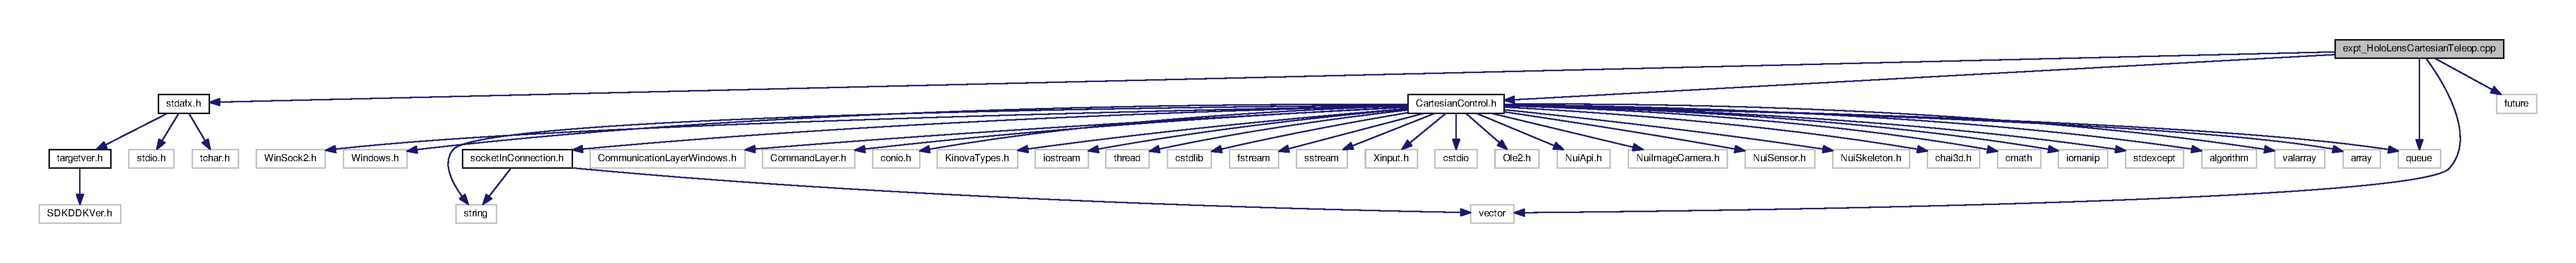
\includegraphics[width=350pt]{da/d5b/expt__HoloLensCartesianTeleop_8cpp__incl}
\end{center}
\end{figure}
\subsection*{Macros}
\begin{DoxyCompactItemize}
\item 
\#define \hyperlink{expt__HoloLensCartesianTeleop_8cpp_a5762b99b606a8008d4244c4d484e1f1c}{T\+R\+A\+IN}~true
\item 
\#define \hyperlink{expt__HoloLensCartesianTeleop_8cpp_a864a52c772f23a04bcef46a40c9efed4}{T\+E\+S\+T\+\_\+1}~false
\item 
\#define \hyperlink{expt__HoloLensCartesianTeleop_8cpp_aa97013921b0b86f7b58de46505cd223b}{T\+E\+S\+T\+\_\+2}~false
\item 
\#define \hyperlink{expt__HoloLensCartesianTeleop_8cpp_ac86054dc8d23e66c9556657b04e2a5f3}{I\+N\+V\+E\+R\+S\+E\+\_\+\+C\+O\+N\+T\+R\+O\+L\+L\+ER}~false
\item 
\#define \hyperlink{expt__HoloLensCartesianTeleop_8cpp_ace138276390387cfa2180f589e502f82}{L\+O\+A\+D\+\_\+\+U\+H\+X\+\_\+\+F\+R\+O\+M\+\_\+\+F\+I\+LE}~false
\item 
\#define \hyperlink{expt__HoloLensCartesianTeleop_8cpp_a0d517e64a65ae6a5522a96096b29ee6b}{L\+O\+A\+D\+\_\+\+X\+M\+\_\+\+F\+R\+O\+M\+\_\+\+F\+I\+LE}~false
\end{DoxyCompactItemize}
\subsection*{Variables}
\begin{DoxyCompactItemize}
\item 
\hyperlink{classNovintFalconHapticsDevice}{Novint\+Falcon\+Haptics\+Device} $\ast$ \hyperlink{expt__HoloLensCartesianTeleop_8cpp_a5af8a150b7e3676a29b7844262dd4d6f}{novint\+Falcon} = new \hyperlink{classNovintFalconHapticsDevice}{Novint\+Falcon\+Haptics\+Device}
\end{DoxyCompactItemize}


\subsection{Macro Definition Documentation}
\index{expt\+\_\+\+Holo\+Lens\+Cartesian\+Teleop.\+cpp@{expt\+\_\+\+Holo\+Lens\+Cartesian\+Teleop.\+cpp}!I\+N\+V\+E\+R\+S\+E\+\_\+\+C\+O\+N\+T\+R\+O\+L\+L\+ER@{I\+N\+V\+E\+R\+S\+E\+\_\+\+C\+O\+N\+T\+R\+O\+L\+L\+ER}}
\index{I\+N\+V\+E\+R\+S\+E\+\_\+\+C\+O\+N\+T\+R\+O\+L\+L\+ER@{I\+N\+V\+E\+R\+S\+E\+\_\+\+C\+O\+N\+T\+R\+O\+L\+L\+ER}!expt\+\_\+\+Holo\+Lens\+Cartesian\+Teleop.\+cpp@{expt\+\_\+\+Holo\+Lens\+Cartesian\+Teleop.\+cpp}}
\subsubsection[{\texorpdfstring{I\+N\+V\+E\+R\+S\+E\+\_\+\+C\+O\+N\+T\+R\+O\+L\+L\+ER}{INVERSE_CONTROLLER}}]{\setlength{\rightskip}{0pt plus 5cm}\#define I\+N\+V\+E\+R\+S\+E\+\_\+\+C\+O\+N\+T\+R\+O\+L\+L\+ER~false}\hypertarget{expt__HoloLensCartesianTeleop_8cpp_ac86054dc8d23e66c9556657b04e2a5f3}{}\label{expt__HoloLensCartesianTeleop_8cpp_ac86054dc8d23e66c9556657b04e2a5f3}
\index{expt\+\_\+\+Holo\+Lens\+Cartesian\+Teleop.\+cpp@{expt\+\_\+\+Holo\+Lens\+Cartesian\+Teleop.\+cpp}!L\+O\+A\+D\+\_\+\+U\+H\+X\+\_\+\+F\+R\+O\+M\+\_\+\+F\+I\+LE@{L\+O\+A\+D\+\_\+\+U\+H\+X\+\_\+\+F\+R\+O\+M\+\_\+\+F\+I\+LE}}
\index{L\+O\+A\+D\+\_\+\+U\+H\+X\+\_\+\+F\+R\+O\+M\+\_\+\+F\+I\+LE@{L\+O\+A\+D\+\_\+\+U\+H\+X\+\_\+\+F\+R\+O\+M\+\_\+\+F\+I\+LE}!expt\+\_\+\+Holo\+Lens\+Cartesian\+Teleop.\+cpp@{expt\+\_\+\+Holo\+Lens\+Cartesian\+Teleop.\+cpp}}
\subsubsection[{\texorpdfstring{L\+O\+A\+D\+\_\+\+U\+H\+X\+\_\+\+F\+R\+O\+M\+\_\+\+F\+I\+LE}{LOAD_UHX_FROM_FILE}}]{\setlength{\rightskip}{0pt plus 5cm}\#define L\+O\+A\+D\+\_\+\+U\+H\+X\+\_\+\+F\+R\+O\+M\+\_\+\+F\+I\+LE~false}\hypertarget{expt__HoloLensCartesianTeleop_8cpp_ace138276390387cfa2180f589e502f82}{}\label{expt__HoloLensCartesianTeleop_8cpp_ace138276390387cfa2180f589e502f82}
\index{expt\+\_\+\+Holo\+Lens\+Cartesian\+Teleop.\+cpp@{expt\+\_\+\+Holo\+Lens\+Cartesian\+Teleop.\+cpp}!L\+O\+A\+D\+\_\+\+X\+M\+\_\+\+F\+R\+O\+M\+\_\+\+F\+I\+LE@{L\+O\+A\+D\+\_\+\+X\+M\+\_\+\+F\+R\+O\+M\+\_\+\+F\+I\+LE}}
\index{L\+O\+A\+D\+\_\+\+X\+M\+\_\+\+F\+R\+O\+M\+\_\+\+F\+I\+LE@{L\+O\+A\+D\+\_\+\+X\+M\+\_\+\+F\+R\+O\+M\+\_\+\+F\+I\+LE}!expt\+\_\+\+Holo\+Lens\+Cartesian\+Teleop.\+cpp@{expt\+\_\+\+Holo\+Lens\+Cartesian\+Teleop.\+cpp}}
\subsubsection[{\texorpdfstring{L\+O\+A\+D\+\_\+\+X\+M\+\_\+\+F\+R\+O\+M\+\_\+\+F\+I\+LE}{LOAD_XM_FROM_FILE}}]{\setlength{\rightskip}{0pt plus 5cm}\#define L\+O\+A\+D\+\_\+\+X\+M\+\_\+\+F\+R\+O\+M\+\_\+\+F\+I\+LE~false}\hypertarget{expt__HoloLensCartesianTeleop_8cpp_a0d517e64a65ae6a5522a96096b29ee6b}{}\label{expt__HoloLensCartesianTeleop_8cpp_a0d517e64a65ae6a5522a96096b29ee6b}
\index{expt\+\_\+\+Holo\+Lens\+Cartesian\+Teleop.\+cpp@{expt\+\_\+\+Holo\+Lens\+Cartesian\+Teleop.\+cpp}!T\+E\+S\+T\+\_\+1@{T\+E\+S\+T\+\_\+1}}
\index{T\+E\+S\+T\+\_\+1@{T\+E\+S\+T\+\_\+1}!expt\+\_\+\+Holo\+Lens\+Cartesian\+Teleop.\+cpp@{expt\+\_\+\+Holo\+Lens\+Cartesian\+Teleop.\+cpp}}
\subsubsection[{\texorpdfstring{T\+E\+S\+T\+\_\+1}{TEST_1}}]{\setlength{\rightskip}{0pt plus 5cm}\#define T\+E\+S\+T\+\_\+1~false}\hypertarget{expt__HoloLensCartesianTeleop_8cpp_a864a52c772f23a04bcef46a40c9efed4}{}\label{expt__HoloLensCartesianTeleop_8cpp_a864a52c772f23a04bcef46a40c9efed4}
\index{expt\+\_\+\+Holo\+Lens\+Cartesian\+Teleop.\+cpp@{expt\+\_\+\+Holo\+Lens\+Cartesian\+Teleop.\+cpp}!T\+E\+S\+T\+\_\+2@{T\+E\+S\+T\+\_\+2}}
\index{T\+E\+S\+T\+\_\+2@{T\+E\+S\+T\+\_\+2}!expt\+\_\+\+Holo\+Lens\+Cartesian\+Teleop.\+cpp@{expt\+\_\+\+Holo\+Lens\+Cartesian\+Teleop.\+cpp}}
\subsubsection[{\texorpdfstring{T\+E\+S\+T\+\_\+2}{TEST_2}}]{\setlength{\rightskip}{0pt plus 5cm}\#define T\+E\+S\+T\+\_\+2~false}\hypertarget{expt__HoloLensCartesianTeleop_8cpp_aa97013921b0b86f7b58de46505cd223b}{}\label{expt__HoloLensCartesianTeleop_8cpp_aa97013921b0b86f7b58de46505cd223b}
\index{expt\+\_\+\+Holo\+Lens\+Cartesian\+Teleop.\+cpp@{expt\+\_\+\+Holo\+Lens\+Cartesian\+Teleop.\+cpp}!T\+R\+A\+IN@{T\+R\+A\+IN}}
\index{T\+R\+A\+IN@{T\+R\+A\+IN}!expt\+\_\+\+Holo\+Lens\+Cartesian\+Teleop.\+cpp@{expt\+\_\+\+Holo\+Lens\+Cartesian\+Teleop.\+cpp}}
\subsubsection[{\texorpdfstring{T\+R\+A\+IN}{TRAIN}}]{\setlength{\rightskip}{0pt plus 5cm}\#define T\+R\+A\+IN~true}\hypertarget{expt__HoloLensCartesianTeleop_8cpp_a5762b99b606a8008d4244c4d484e1f1c}{}\label{expt__HoloLensCartesianTeleop_8cpp_a5762b99b606a8008d4244c4d484e1f1c}


\subsection{Variable Documentation}
\index{expt\+\_\+\+Holo\+Lens\+Cartesian\+Teleop.\+cpp@{expt\+\_\+\+Holo\+Lens\+Cartesian\+Teleop.\+cpp}!novint\+Falcon@{novint\+Falcon}}
\index{novint\+Falcon@{novint\+Falcon}!expt\+\_\+\+Holo\+Lens\+Cartesian\+Teleop.\+cpp@{expt\+\_\+\+Holo\+Lens\+Cartesian\+Teleop.\+cpp}}
\subsubsection[{\texorpdfstring{novint\+Falcon}{novintFalcon}}]{\setlength{\rightskip}{0pt plus 5cm}{\bf Novint\+Falcon\+Haptics\+Device}$\ast$ novint\+Falcon = new {\bf Novint\+Falcon\+Haptics\+Device}}\hypertarget{expt__HoloLensCartesianTeleop_8cpp_a5af8a150b7e3676a29b7844262dd4d6f}{}\label{expt__HoloLensCartesianTeleop_8cpp_a5af8a150b7e3676a29b7844262dd4d6f}

\hypertarget{KinovaHMICartesianControl_2expt__HoloLensCartesianTeleop_8cpp}{}\section{expt\+\_\+\+Holo\+Lens\+Cartesian\+Teleop.\+cpp File Reference}
\label{KinovaHMICartesianControl_2expt__HoloLensCartesianTeleop_8cpp}\index{expt\+\_\+\+Holo\+Lens\+Cartesian\+Teleop.\+cpp@{expt\+\_\+\+Holo\+Lens\+Cartesian\+Teleop.\+cpp}}
{\ttfamily \#include \char`\"{}stdafx.\+h\char`\"{}}\\*
{\ttfamily \#include \char`\"{}Cartesian\+Control.\+h\char`\"{}}\\*
{\ttfamily \#include $<$vector$>$}\\*
{\ttfamily \#include $<$queue$>$}\\*
{\ttfamily \#include $<$future$>$}\\*
Include dependency graph for Kinova\+H\+M\+I\+Cartesian\+Control/expt\+\_\+\+Holo\+Lens\+Cartesian\+Teleop.cpp\+:
\nopagebreak
\begin{figure}[H]
\begin{center}
\leavevmode
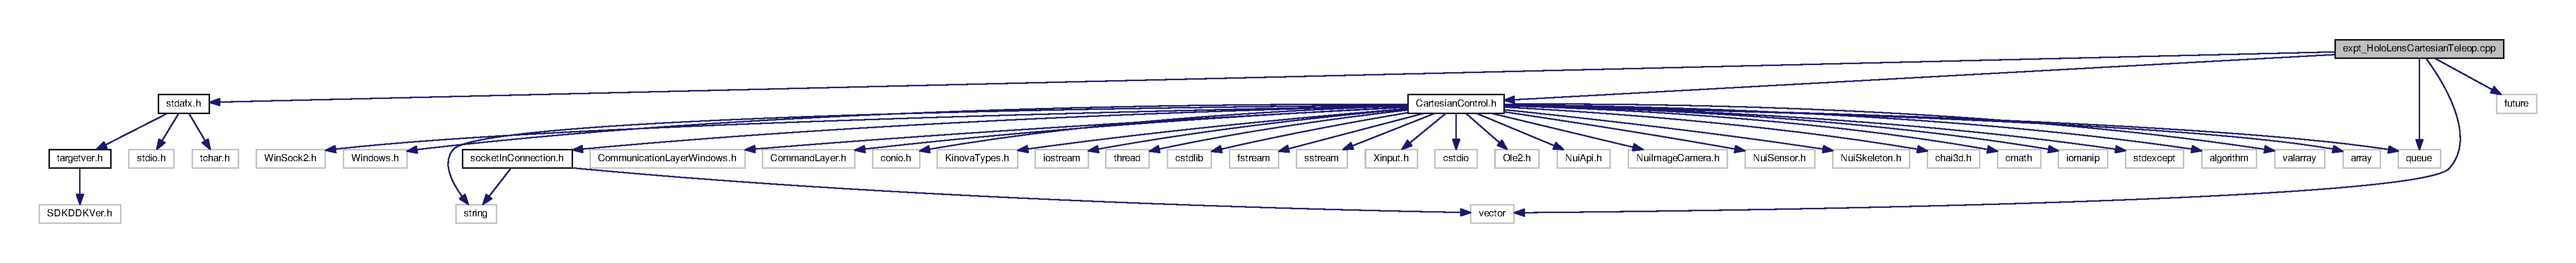
\includegraphics[width=350pt]{db/dbc/KinovaHMICartesianControl_2expt__HoloLensCartesianTeleop_8cpp__incl}
\end{center}
\end{figure}
\subsection*{Macros}
\begin{DoxyCompactItemize}
\item 
\#define \hyperlink{KinovaHMICartesianControl_2expt__HoloLensCartesianTeleop_8cpp_a5762b99b606a8008d4244c4d484e1f1c}{T\+R\+A\+IN}~true
\item 
\#define \hyperlink{KinovaHMICartesianControl_2expt__HoloLensCartesianTeleop_8cpp_a864a52c772f23a04bcef46a40c9efed4}{T\+E\+S\+T\+\_\+1}~false
\item 
\#define \hyperlink{KinovaHMICartesianControl_2expt__HoloLensCartesianTeleop_8cpp_aa97013921b0b86f7b58de46505cd223b}{T\+E\+S\+T\+\_\+2}~false
\item 
\#define \hyperlink{KinovaHMICartesianControl_2expt__HoloLensCartesianTeleop_8cpp_ac86054dc8d23e66c9556657b04e2a5f3}{I\+N\+V\+E\+R\+S\+E\+\_\+\+C\+O\+N\+T\+R\+O\+L\+L\+ER}~false
\item 
\#define \hyperlink{KinovaHMICartesianControl_2expt__HoloLensCartesianTeleop_8cpp_ace138276390387cfa2180f589e502f82}{L\+O\+A\+D\+\_\+\+U\+H\+X\+\_\+\+F\+R\+O\+M\+\_\+\+F\+I\+LE}~false
\item 
\#define \hyperlink{KinovaHMICartesianControl_2expt__HoloLensCartesianTeleop_8cpp_a0d517e64a65ae6a5522a96096b29ee6b}{L\+O\+A\+D\+\_\+\+X\+M\+\_\+\+F\+R\+O\+M\+\_\+\+F\+I\+LE}~false
\end{DoxyCompactItemize}
\subsection*{Variables}
\begin{DoxyCompactItemize}
\item 
\hyperlink{classNovintFalconHapticsDevice}{Novint\+Falcon\+Haptics\+Device} $\ast$ \hyperlink{KinovaHMICartesianControl_2expt__HoloLensCartesianTeleop_8cpp_a5af8a150b7e3676a29b7844262dd4d6f}{novint\+Falcon} = new \hyperlink{classNovintFalconHapticsDevice}{Novint\+Falcon\+Haptics\+Device}
\end{DoxyCompactItemize}


\subsection{Macro Definition Documentation}
\index{Kinova\+H\+M\+I\+Cartesian\+Control/expt\+\_\+\+Holo\+Lens\+Cartesian\+Teleop.\+cpp@{Kinova\+H\+M\+I\+Cartesian\+Control/expt\+\_\+\+Holo\+Lens\+Cartesian\+Teleop.\+cpp}!I\+N\+V\+E\+R\+S\+E\+\_\+\+C\+O\+N\+T\+R\+O\+L\+L\+ER@{I\+N\+V\+E\+R\+S\+E\+\_\+\+C\+O\+N\+T\+R\+O\+L\+L\+ER}}
\index{I\+N\+V\+E\+R\+S\+E\+\_\+\+C\+O\+N\+T\+R\+O\+L\+L\+ER@{I\+N\+V\+E\+R\+S\+E\+\_\+\+C\+O\+N\+T\+R\+O\+L\+L\+ER}!Kinova\+H\+M\+I\+Cartesian\+Control/expt\+\_\+\+Holo\+Lens\+Cartesian\+Teleop.\+cpp@{Kinova\+H\+M\+I\+Cartesian\+Control/expt\+\_\+\+Holo\+Lens\+Cartesian\+Teleop.\+cpp}}
\subsubsection[{\texorpdfstring{I\+N\+V\+E\+R\+S\+E\+\_\+\+C\+O\+N\+T\+R\+O\+L\+L\+ER}{INVERSE_CONTROLLER}}]{\setlength{\rightskip}{0pt plus 5cm}\#define I\+N\+V\+E\+R\+S\+E\+\_\+\+C\+O\+N\+T\+R\+O\+L\+L\+ER~false}\hypertarget{KinovaHMICartesianControl_2expt__HoloLensCartesianTeleop_8cpp_ac86054dc8d23e66c9556657b04e2a5f3}{}\label{KinovaHMICartesianControl_2expt__HoloLensCartesianTeleop_8cpp_ac86054dc8d23e66c9556657b04e2a5f3}
\index{Kinova\+H\+M\+I\+Cartesian\+Control/expt\+\_\+\+Holo\+Lens\+Cartesian\+Teleop.\+cpp@{Kinova\+H\+M\+I\+Cartesian\+Control/expt\+\_\+\+Holo\+Lens\+Cartesian\+Teleop.\+cpp}!L\+O\+A\+D\+\_\+\+U\+H\+X\+\_\+\+F\+R\+O\+M\+\_\+\+F\+I\+LE@{L\+O\+A\+D\+\_\+\+U\+H\+X\+\_\+\+F\+R\+O\+M\+\_\+\+F\+I\+LE}}
\index{L\+O\+A\+D\+\_\+\+U\+H\+X\+\_\+\+F\+R\+O\+M\+\_\+\+F\+I\+LE@{L\+O\+A\+D\+\_\+\+U\+H\+X\+\_\+\+F\+R\+O\+M\+\_\+\+F\+I\+LE}!Kinova\+H\+M\+I\+Cartesian\+Control/expt\+\_\+\+Holo\+Lens\+Cartesian\+Teleop.\+cpp@{Kinova\+H\+M\+I\+Cartesian\+Control/expt\+\_\+\+Holo\+Lens\+Cartesian\+Teleop.\+cpp}}
\subsubsection[{\texorpdfstring{L\+O\+A\+D\+\_\+\+U\+H\+X\+\_\+\+F\+R\+O\+M\+\_\+\+F\+I\+LE}{LOAD_UHX_FROM_FILE}}]{\setlength{\rightskip}{0pt plus 5cm}\#define L\+O\+A\+D\+\_\+\+U\+H\+X\+\_\+\+F\+R\+O\+M\+\_\+\+F\+I\+LE~false}\hypertarget{KinovaHMICartesianControl_2expt__HoloLensCartesianTeleop_8cpp_ace138276390387cfa2180f589e502f82}{}\label{KinovaHMICartesianControl_2expt__HoloLensCartesianTeleop_8cpp_ace138276390387cfa2180f589e502f82}
\index{Kinova\+H\+M\+I\+Cartesian\+Control/expt\+\_\+\+Holo\+Lens\+Cartesian\+Teleop.\+cpp@{Kinova\+H\+M\+I\+Cartesian\+Control/expt\+\_\+\+Holo\+Lens\+Cartesian\+Teleop.\+cpp}!L\+O\+A\+D\+\_\+\+X\+M\+\_\+\+F\+R\+O\+M\+\_\+\+F\+I\+LE@{L\+O\+A\+D\+\_\+\+X\+M\+\_\+\+F\+R\+O\+M\+\_\+\+F\+I\+LE}}
\index{L\+O\+A\+D\+\_\+\+X\+M\+\_\+\+F\+R\+O\+M\+\_\+\+F\+I\+LE@{L\+O\+A\+D\+\_\+\+X\+M\+\_\+\+F\+R\+O\+M\+\_\+\+F\+I\+LE}!Kinova\+H\+M\+I\+Cartesian\+Control/expt\+\_\+\+Holo\+Lens\+Cartesian\+Teleop.\+cpp@{Kinova\+H\+M\+I\+Cartesian\+Control/expt\+\_\+\+Holo\+Lens\+Cartesian\+Teleop.\+cpp}}
\subsubsection[{\texorpdfstring{L\+O\+A\+D\+\_\+\+X\+M\+\_\+\+F\+R\+O\+M\+\_\+\+F\+I\+LE}{LOAD_XM_FROM_FILE}}]{\setlength{\rightskip}{0pt plus 5cm}\#define L\+O\+A\+D\+\_\+\+X\+M\+\_\+\+F\+R\+O\+M\+\_\+\+F\+I\+LE~false}\hypertarget{KinovaHMICartesianControl_2expt__HoloLensCartesianTeleop_8cpp_a0d517e64a65ae6a5522a96096b29ee6b}{}\label{KinovaHMICartesianControl_2expt__HoloLensCartesianTeleop_8cpp_a0d517e64a65ae6a5522a96096b29ee6b}
\index{Kinova\+H\+M\+I\+Cartesian\+Control/expt\+\_\+\+Holo\+Lens\+Cartesian\+Teleop.\+cpp@{Kinova\+H\+M\+I\+Cartesian\+Control/expt\+\_\+\+Holo\+Lens\+Cartesian\+Teleop.\+cpp}!T\+E\+S\+T\+\_\+1@{T\+E\+S\+T\+\_\+1}}
\index{T\+E\+S\+T\+\_\+1@{T\+E\+S\+T\+\_\+1}!Kinova\+H\+M\+I\+Cartesian\+Control/expt\+\_\+\+Holo\+Lens\+Cartesian\+Teleop.\+cpp@{Kinova\+H\+M\+I\+Cartesian\+Control/expt\+\_\+\+Holo\+Lens\+Cartesian\+Teleop.\+cpp}}
\subsubsection[{\texorpdfstring{T\+E\+S\+T\+\_\+1}{TEST_1}}]{\setlength{\rightskip}{0pt plus 5cm}\#define T\+E\+S\+T\+\_\+1~false}\hypertarget{KinovaHMICartesianControl_2expt__HoloLensCartesianTeleop_8cpp_a864a52c772f23a04bcef46a40c9efed4}{}\label{KinovaHMICartesianControl_2expt__HoloLensCartesianTeleop_8cpp_a864a52c772f23a04bcef46a40c9efed4}
\index{Kinova\+H\+M\+I\+Cartesian\+Control/expt\+\_\+\+Holo\+Lens\+Cartesian\+Teleop.\+cpp@{Kinova\+H\+M\+I\+Cartesian\+Control/expt\+\_\+\+Holo\+Lens\+Cartesian\+Teleop.\+cpp}!T\+E\+S\+T\+\_\+2@{T\+E\+S\+T\+\_\+2}}
\index{T\+E\+S\+T\+\_\+2@{T\+E\+S\+T\+\_\+2}!Kinova\+H\+M\+I\+Cartesian\+Control/expt\+\_\+\+Holo\+Lens\+Cartesian\+Teleop.\+cpp@{Kinova\+H\+M\+I\+Cartesian\+Control/expt\+\_\+\+Holo\+Lens\+Cartesian\+Teleop.\+cpp}}
\subsubsection[{\texorpdfstring{T\+E\+S\+T\+\_\+2}{TEST_2}}]{\setlength{\rightskip}{0pt plus 5cm}\#define T\+E\+S\+T\+\_\+2~false}\hypertarget{KinovaHMICartesianControl_2expt__HoloLensCartesianTeleop_8cpp_aa97013921b0b86f7b58de46505cd223b}{}\label{KinovaHMICartesianControl_2expt__HoloLensCartesianTeleop_8cpp_aa97013921b0b86f7b58de46505cd223b}
\index{Kinova\+H\+M\+I\+Cartesian\+Control/expt\+\_\+\+Holo\+Lens\+Cartesian\+Teleop.\+cpp@{Kinova\+H\+M\+I\+Cartesian\+Control/expt\+\_\+\+Holo\+Lens\+Cartesian\+Teleop.\+cpp}!T\+R\+A\+IN@{T\+R\+A\+IN}}
\index{T\+R\+A\+IN@{T\+R\+A\+IN}!Kinova\+H\+M\+I\+Cartesian\+Control/expt\+\_\+\+Holo\+Lens\+Cartesian\+Teleop.\+cpp@{Kinova\+H\+M\+I\+Cartesian\+Control/expt\+\_\+\+Holo\+Lens\+Cartesian\+Teleop.\+cpp}}
\subsubsection[{\texorpdfstring{T\+R\+A\+IN}{TRAIN}}]{\setlength{\rightskip}{0pt plus 5cm}\#define T\+R\+A\+IN~true}\hypertarget{KinovaHMICartesianControl_2expt__HoloLensCartesianTeleop_8cpp_a5762b99b606a8008d4244c4d484e1f1c}{}\label{KinovaHMICartesianControl_2expt__HoloLensCartesianTeleop_8cpp_a5762b99b606a8008d4244c4d484e1f1c}


\subsection{Variable Documentation}
\index{Kinova\+H\+M\+I\+Cartesian\+Control/expt\+\_\+\+Holo\+Lens\+Cartesian\+Teleop.\+cpp@{Kinova\+H\+M\+I\+Cartesian\+Control/expt\+\_\+\+Holo\+Lens\+Cartesian\+Teleop.\+cpp}!novint\+Falcon@{novint\+Falcon}}
\index{novint\+Falcon@{novint\+Falcon}!Kinova\+H\+M\+I\+Cartesian\+Control/expt\+\_\+\+Holo\+Lens\+Cartesian\+Teleop.\+cpp@{Kinova\+H\+M\+I\+Cartesian\+Control/expt\+\_\+\+Holo\+Lens\+Cartesian\+Teleop.\+cpp}}
\subsubsection[{\texorpdfstring{novint\+Falcon}{novintFalcon}}]{\setlength{\rightskip}{0pt plus 5cm}{\bf Novint\+Falcon\+Haptics\+Device}$\ast$ novint\+Falcon = new {\bf Novint\+Falcon\+Haptics\+Device}}\hypertarget{KinovaHMICartesianControl_2expt__HoloLensCartesianTeleop_8cpp_a5af8a150b7e3676a29b7844262dd4d6f}{}\label{KinovaHMICartesianControl_2expt__HoloLensCartesianTeleop_8cpp_a5af8a150b7e3676a29b7844262dd4d6f}

\hypertarget{files__0_8js}{}\section{files\+\_\+0.\+js File Reference}
\label{files__0_8js}\index{files\+\_\+0.\+js@{files\+\_\+0.\+js}}
\subsection*{Variables}
\begin{DoxyCompactItemize}
\item 
var \hyperlink{files__0_8js_ad01a7523f103d6242ef9b0451861231e}{search\+Data}
\end{DoxyCompactItemize}


\subsection{Variable Documentation}
\index{files\+\_\+0.\+js@{files\+\_\+0.\+js}!search\+Data@{search\+Data}}
\index{search\+Data@{search\+Data}!files\+\_\+0.\+js@{files\+\_\+0.\+js}}
\subsubsection[{\texorpdfstring{search\+Data}{searchData}}]{\setlength{\rightskip}{0pt plus 5cm}var search\+Data}\hypertarget{files__0_8js_ad01a7523f103d6242ef9b0451861231e}{}\label{files__0_8js_ad01a7523f103d6242ef9b0451861231e}
{\bfseries Initial value\+:}
\begin{DoxyCode}
=
[
  [\textcolor{stringliteral}{'angularcommandcontrol\_2ecpp'},[\textcolor{stringliteral}{'angularCommandControl.cpp'},[\textcolor{stringliteral}{'../d2/d77/angularCommandControl\_8cpp.html'},
      1,\textcolor{stringliteral}{''}]]]
]
\end{DoxyCode}

\hypertarget{files__1_8js}{}\section{files\+\_\+1.\+js File Reference}
\label{files__1_8js}\index{files\+\_\+1.\+js@{files\+\_\+1.\+js}}
\subsection*{Variables}
\begin{DoxyCompactItemize}
\item 
var \hyperlink{files__1_8js_ad01a7523f103d6242ef9b0451861231e}{search\+Data}
\end{DoxyCompactItemize}


\subsection{Variable Documentation}
\index{files\+\_\+1.\+js@{files\+\_\+1.\+js}!search\+Data@{search\+Data}}
\index{search\+Data@{search\+Data}!files\+\_\+1.\+js@{files\+\_\+1.\+js}}
\subsubsection[{\texorpdfstring{search\+Data}{searchData}}]{\setlength{\rightskip}{0pt plus 5cm}var search\+Data}\hypertarget{files__1_8js_ad01a7523f103d6242ef9b0451861231e}{}\label{files__1_8js_ad01a7523f103d6242ef9b0451861231e}
{\bfseries Initial value\+:}
\begin{DoxyCode}
=
[
  [\textcolor{stringliteral}{'cartesiancontrol\_2eh'},[\textcolor{stringliteral}{'CartesianControl.h'},[\textcolor{stringliteral}{'../da/d2f/CartesianControl\_8h.html'},1,\textcolor{stringliteral}{''}]]]
]
\end{DoxyCode}

\hypertarget{files__2_8js}{}\section{files\+\_\+2.\+js File Reference}
\label{files__2_8js}\index{files\+\_\+2.\+js@{files\+\_\+2.\+js}}
\subsection*{Variables}
\begin{DoxyCompactItemize}
\item 
var \hyperlink{files__2_8js_ad01a7523f103d6242ef9b0451861231e}{search\+Data}
\end{DoxyCompactItemize}


\subsection{Variable Documentation}
\index{files\+\_\+2.\+js@{files\+\_\+2.\+js}!search\+Data@{search\+Data}}
\index{search\+Data@{search\+Data}!files\+\_\+2.\+js@{files\+\_\+2.\+js}}
\subsubsection[{\texorpdfstring{search\+Data}{searchData}}]{\setlength{\rightskip}{0pt plus 5cm}var search\+Data}\hypertarget{files__2_8js_ad01a7523f103d6242ef9b0451861231e}{}\label{files__2_8js_ad01a7523f103d6242ef9b0451861231e}
{\bfseries Initial value\+:}
\begin{DoxyCode}
=
[
  [\textcolor{stringliteral}{'expt\_5fhololenscartesianteleop\_2ecpp'},[\textcolor{stringliteral}{'expt\_HoloLensCartesianTeleop.cpp'},[\textcolor{stringliteral}{'
      ../d2/d39/expt\_\_HoloLensCartesianTeleop\_8cpp.html'},1,\textcolor{stringliteral}{''}]]]
]
\end{DoxyCode}

\hypertarget{files__3_8js}{}\section{files\+\_\+3.\+js File Reference}
\label{files__3_8js}\index{files\+\_\+3.\+js@{files\+\_\+3.\+js}}
\subsection*{Variables}
\begin{DoxyCompactItemize}
\item 
var \hyperlink{files__3_8js_ad01a7523f103d6242ef9b0451861231e}{search\+Data}
\end{DoxyCompactItemize}


\subsection{Variable Documentation}
\index{files\+\_\+3.\+js@{files\+\_\+3.\+js}!search\+Data@{search\+Data}}
\index{search\+Data@{search\+Data}!files\+\_\+3.\+js@{files\+\_\+3.\+js}}
\subsubsection[{\texorpdfstring{search\+Data}{searchData}}]{\setlength{\rightskip}{0pt plus 5cm}var search\+Data}\hypertarget{files__3_8js_ad01a7523f103d6242ef9b0451861231e}{}\label{files__3_8js_ad01a7523f103d6242ef9b0451861231e}
{\bfseries Initial value\+:}
\begin{DoxyCode}
=
[
  [\textcolor{stringliteral}{'firfilter\_2ecpp'},[\textcolor{stringliteral}{'firFilter.cpp'},[\textcolor{stringliteral}{'../d2/de6/firFilter\_8cpp.html'},1,\textcolor{stringliteral}{''}]]]
]
\end{DoxyCode}

\hypertarget{files__4_8js}{}\section{files\+\_\+4.\+js File Reference}
\label{files__4_8js}\index{files\+\_\+4.\+js@{files\+\_\+4.\+js}}
\subsection*{Variables}
\begin{DoxyCompactItemize}
\item 
var \hyperlink{files__4_8js_ad01a7523f103d6242ef9b0451861231e}{search\+Data}
\end{DoxyCompactItemize}


\subsection{Variable Documentation}
\index{files\+\_\+4.\+js@{files\+\_\+4.\+js}!search\+Data@{search\+Data}}
\index{search\+Data@{search\+Data}!files\+\_\+4.\+js@{files\+\_\+4.\+js}}
\subsubsection[{\texorpdfstring{search\+Data}{searchData}}]{\setlength{\rightskip}{0pt plus 5cm}var search\+Data}\hypertarget{files__4_8js_ad01a7523f103d6242ef9b0451861231e}{}\label{files__4_8js_ad01a7523f103d6242ef9b0451861231e}
{\bfseries Initial value\+:}
\begin{DoxyCode}
=
[
  [\textcolor{stringliteral}{'hmifunctions\_2ecpp'},[\textcolor{stringliteral}{'HMIfunctions.cpp'},[\textcolor{stringliteral}{'../d9/dd2/HMIfunctions\_8cpp.html'},1,\textcolor{stringliteral}{''}]]]
]
\end{DoxyCode}

\hypertarget{files__5_8js}{}\section{files\+\_\+5.\+js File Reference}
\label{files__5_8js}\index{files\+\_\+5.\+js@{files\+\_\+5.\+js}}
\subsection*{Variables}
\begin{DoxyCompactItemize}
\item 
var \hyperlink{files__5_8js_ad01a7523f103d6242ef9b0451861231e}{search\+Data}
\end{DoxyCompactItemize}


\subsection{Variable Documentation}
\index{files\+\_\+5.\+js@{files\+\_\+5.\+js}!search\+Data@{search\+Data}}
\index{search\+Data@{search\+Data}!files\+\_\+5.\+js@{files\+\_\+5.\+js}}
\subsubsection[{\texorpdfstring{search\+Data}{searchData}}]{\setlength{\rightskip}{0pt plus 5cm}var search\+Data}\hypertarget{files__5_8js_ad01a7523f103d6242ef9b0451861231e}{}\label{files__5_8js_ad01a7523f103d6242ef9b0451861231e}
{\bfseries Initial value\+:}
\begin{DoxyCode}
=
[
  [\textcolor{stringliteral}{'kinovahmicartesiancontrol\_2ecpp'},[\textcolor{stringliteral}{'KinovaHMICartesianControl.cpp'},[\textcolor{stringliteral}{'
      ../d0/da0/KinovaHMICartesianControl\_8cpp.html'},1,\textcolor{stringliteral}{''}]]]
]
\end{DoxyCode}

\hypertarget{files__6_8js}{}\section{files\+\_\+6.\+js File Reference}
\label{files__6_8js}\index{files\+\_\+6.\+js@{files\+\_\+6.\+js}}
\subsection*{Variables}
\begin{DoxyCompactItemize}
\item 
var \hyperlink{files__6_8js_ad01a7523f103d6242ef9b0451861231e}{search\+Data}
\end{DoxyCompactItemize}


\subsection{Variable Documentation}
\index{files\+\_\+6.\+js@{files\+\_\+6.\+js}!search\+Data@{search\+Data}}
\index{search\+Data@{search\+Data}!files\+\_\+6.\+js@{files\+\_\+6.\+js}}
\subsubsection[{\texorpdfstring{search\+Data}{searchData}}]{\setlength{\rightskip}{0pt plus 5cm}var search\+Data}\hypertarget{files__6_8js_ad01a7523f103d6242ef9b0451861231e}{}\label{files__6_8js_ad01a7523f103d6242ef9b0451861231e}
{\bfseries Initial value\+:}
\begin{DoxyCode}
=
[
  [\textcolor{stringliteral}{'lutlinearinterp\_2ecpp'},[\textcolor{stringliteral}{'lutLinearInterp.cpp'},[\textcolor{stringliteral}{'../d0/daf/lutLinearInterp\_8cpp.html'},1,\textcolor{stringliteral}{''}]]]
]
\end{DoxyCode}

\hypertarget{files__7_8js}{}\section{files\+\_\+7.\+js File Reference}
\label{files__7_8js}\index{files\+\_\+7.\+js@{files\+\_\+7.\+js}}
\subsection*{Variables}
\begin{DoxyCompactItemize}
\item 
var \hyperlink{files__7_8js_ad01a7523f103d6242ef9b0451861231e}{search\+Data}
\end{DoxyCompactItemize}


\subsection{Variable Documentation}
\index{files\+\_\+7.\+js@{files\+\_\+7.\+js}!search\+Data@{search\+Data}}
\index{search\+Data@{search\+Data}!files\+\_\+7.\+js@{files\+\_\+7.\+js}}
\subsubsection[{\texorpdfstring{search\+Data}{searchData}}]{\setlength{\rightskip}{0pt plus 5cm}var search\+Data}\hypertarget{files__7_8js_ad01a7523f103d6242ef9b0451861231e}{}\label{files__7_8js_ad01a7523f103d6242ef9b0451861231e}
{\bfseries Initial value\+:}
\begin{DoxyCode}
=
[
  [\textcolor{stringliteral}{'socketinconnection\_2ecpp'},[\textcolor{stringliteral}{'socketInConnection.cpp'},[\textcolor{stringliteral}{'../d8/dca/socketInConnection\_8cpp.html'},1,\textcolor{stringliteral}{''}]]],
  [\textcolor{stringliteral}{'socketinconnection\_2eh'},[\textcolor{stringliteral}{'socketInConnection.h'},[\textcolor{stringliteral}{'../d5/daf/socketInConnection\_8h.html'},1,\textcolor{stringliteral}{''}]]],
  [\textcolor{stringliteral}{'socketoutconnection\_2eh'},[\textcolor{stringliteral}{'socketOutConnection.h'},[\textcolor{stringliteral}{'../d1/d3d/socketOutConnection\_8h.html'},1,\textcolor{stringliteral}{''}]]],
  [\textcolor{stringliteral}{'stdafx\_2ecpp'},[\textcolor{stringliteral}{'stdafx.cpp'},[\textcolor{stringliteral}{'../df/d9d/stdafx\_8cpp.html'},1,\textcolor{stringliteral}{''}]]],
  [\textcolor{stringliteral}{'stdafx\_2eh'},[\textcolor{stringliteral}{'stdafx.h'},[\textcolor{stringliteral}{'../db/d06/stdafx\_8h.html'},1,\textcolor{stringliteral}{''}]]]
]
\end{DoxyCode}

\hypertarget{files__8_8js}{}\section{files\+\_\+8.\+js File Reference}
\label{files__8_8js}\index{files\+\_\+8.\+js@{files\+\_\+8.\+js}}
\subsection*{Variables}
\begin{DoxyCompactItemize}
\item 
var \hyperlink{files__8_8js_ad01a7523f103d6242ef9b0451861231e}{search\+Data}
\end{DoxyCompactItemize}


\subsection{Variable Documentation}
\index{files\+\_\+8.\+js@{files\+\_\+8.\+js}!search\+Data@{search\+Data}}
\index{search\+Data@{search\+Data}!files\+\_\+8.\+js@{files\+\_\+8.\+js}}
\subsubsection[{\texorpdfstring{search\+Data}{searchData}}]{\setlength{\rightskip}{0pt plus 5cm}var search\+Data}\hypertarget{files__8_8js_ad01a7523f103d6242ef9b0451861231e}{}\label{files__8_8js_ad01a7523f103d6242ef9b0451861231e}
{\bfseries Initial value\+:}
\begin{DoxyCode}
=
[
  [\textcolor{stringliteral}{'targetver\_2eh'},[\textcolor{stringliteral}{'targetver.h'},[\textcolor{stringliteral}{'../d9/da6/targetver\_8h.html'},1,\textcolor{stringliteral}{''}]]]
]
\end{DoxyCode}

\hypertarget{firFilter_8cpp}{}\section{fir\+Filter.\+cpp File Reference}
\label{firFilter_8cpp}\index{fir\+Filter.\+cpp@{fir\+Filter.\+cpp}}
{\ttfamily \#include \char`\"{}stdafx.\+h\char`\"{}}\\*
{\ttfamily \#include \char`\"{}Cartesian\+Control.\+h\char`\"{}}\\*
Include dependency graph for fir\+Filter.\+cpp\+:\nopagebreak
\begin{figure}[H]
\begin{center}
\leavevmode
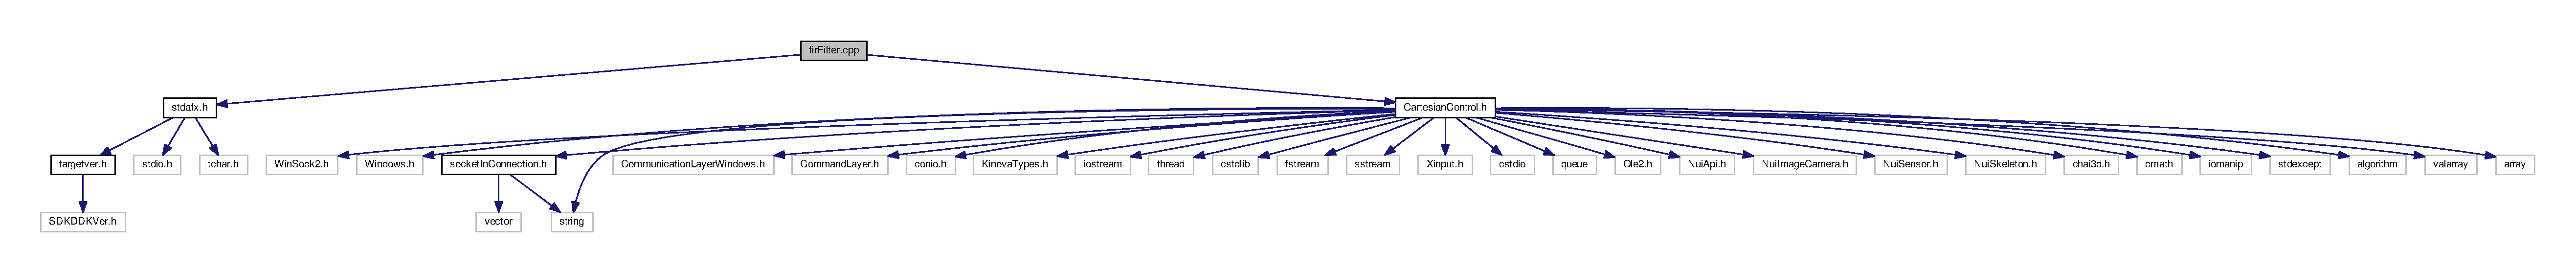
\includegraphics[width=350pt]{d2/d68/firFilter_8cpp__incl}
\end{center}
\end{figure}
\subsection*{Macros}
\begin{DoxyCompactItemize}
\item 
\#define \hyperlink{firFilter_8cpp_adfc8f90f3a8caa8423099cf36ff214f1}{\+\_\+\+W\+I\+N\+S\+O\+C\+K\+\_\+\+D\+E\+P\+R\+E\+C\+A\+T\+E\+D\+\_\+\+N\+O\+\_\+\+W\+A\+R\+N\+I\+N\+GS}
\end{DoxyCompactItemize}


\subsection{Macro Definition Documentation}
\index{fir\+Filter.\+cpp@{fir\+Filter.\+cpp}!\+\_\+\+W\+I\+N\+S\+O\+C\+K\+\_\+\+D\+E\+P\+R\+E\+C\+A\+T\+E\+D\+\_\+\+N\+O\+\_\+\+W\+A\+R\+N\+I\+N\+GS@{\+\_\+\+W\+I\+N\+S\+O\+C\+K\+\_\+\+D\+E\+P\+R\+E\+C\+A\+T\+E\+D\+\_\+\+N\+O\+\_\+\+W\+A\+R\+N\+I\+N\+GS}}
\index{\+\_\+\+W\+I\+N\+S\+O\+C\+K\+\_\+\+D\+E\+P\+R\+E\+C\+A\+T\+E\+D\+\_\+\+N\+O\+\_\+\+W\+A\+R\+N\+I\+N\+GS@{\+\_\+\+W\+I\+N\+S\+O\+C\+K\+\_\+\+D\+E\+P\+R\+E\+C\+A\+T\+E\+D\+\_\+\+N\+O\+\_\+\+W\+A\+R\+N\+I\+N\+GS}!fir\+Filter.\+cpp@{fir\+Filter.\+cpp}}
\subsubsection[{\texorpdfstring{\+\_\+\+W\+I\+N\+S\+O\+C\+K\+\_\+\+D\+E\+P\+R\+E\+C\+A\+T\+E\+D\+\_\+\+N\+O\+\_\+\+W\+A\+R\+N\+I\+N\+GS}{_WINSOCK_DEPRECATED_NO_WARNINGS}}]{\setlength{\rightskip}{0pt plus 5cm}\#define \+\_\+\+W\+I\+N\+S\+O\+C\+K\+\_\+\+D\+E\+P\+R\+E\+C\+A\+T\+E\+D\+\_\+\+N\+O\+\_\+\+W\+A\+R\+N\+I\+N\+GS}\hypertarget{firFilter_8cpp_adfc8f90f3a8caa8423099cf36ff214f1}{}\label{firFilter_8cpp_adfc8f90f3a8caa8423099cf36ff214f1}

\hypertarget{KinovaHMICartesianControl_2firFilter_8cpp}{}\section{fir\+Filter.\+cpp File Reference}
\label{KinovaHMICartesianControl_2firFilter_8cpp}\index{fir\+Filter.\+cpp@{fir\+Filter.\+cpp}}
{\ttfamily \#include \char`\"{}stdafx.\+h\char`\"{}}\\*
{\ttfamily \#include \char`\"{}Cartesian\+Control.\+h\char`\"{}}\\*
Include dependency graph for Kinova\+H\+M\+I\+Cartesian\+Control/fir\+Filter.cpp\+:
\nopagebreak
\begin{figure}[H]
\begin{center}
\leavevmode
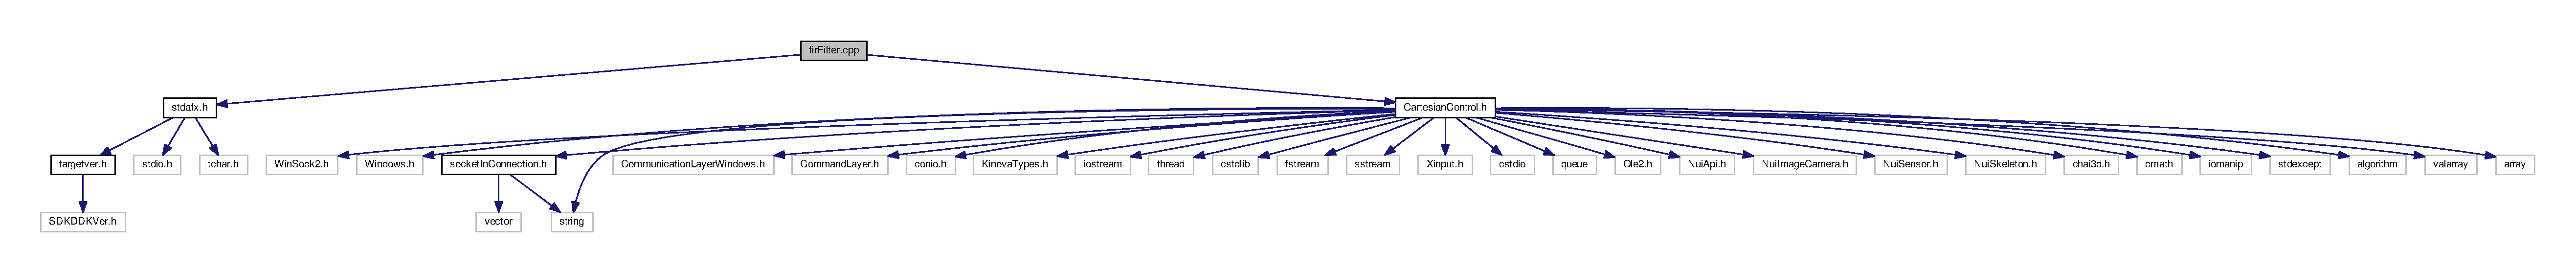
\includegraphics[width=350pt]{dd/df9/KinovaHMICartesianControl_2firFilter_8cpp__incl}
\end{center}
\end{figure}
\subsection*{Macros}
\begin{DoxyCompactItemize}
\item 
\#define \hyperlink{KinovaHMICartesianControl_2firFilter_8cpp_adfc8f90f3a8caa8423099cf36ff214f1}{\+\_\+\+W\+I\+N\+S\+O\+C\+K\+\_\+\+D\+E\+P\+R\+E\+C\+A\+T\+E\+D\+\_\+\+N\+O\+\_\+\+W\+A\+R\+N\+I\+N\+GS}
\end{DoxyCompactItemize}


\subsection{Macro Definition Documentation}
\index{Kinova\+H\+M\+I\+Cartesian\+Control/fir\+Filter.\+cpp@{Kinova\+H\+M\+I\+Cartesian\+Control/fir\+Filter.\+cpp}!\+\_\+\+W\+I\+N\+S\+O\+C\+K\+\_\+\+D\+E\+P\+R\+E\+C\+A\+T\+E\+D\+\_\+\+N\+O\+\_\+\+W\+A\+R\+N\+I\+N\+GS@{\+\_\+\+W\+I\+N\+S\+O\+C\+K\+\_\+\+D\+E\+P\+R\+E\+C\+A\+T\+E\+D\+\_\+\+N\+O\+\_\+\+W\+A\+R\+N\+I\+N\+GS}}
\index{\+\_\+\+W\+I\+N\+S\+O\+C\+K\+\_\+\+D\+E\+P\+R\+E\+C\+A\+T\+E\+D\+\_\+\+N\+O\+\_\+\+W\+A\+R\+N\+I\+N\+GS@{\+\_\+\+W\+I\+N\+S\+O\+C\+K\+\_\+\+D\+E\+P\+R\+E\+C\+A\+T\+E\+D\+\_\+\+N\+O\+\_\+\+W\+A\+R\+N\+I\+N\+GS}!Kinova\+H\+M\+I\+Cartesian\+Control/fir\+Filter.\+cpp@{Kinova\+H\+M\+I\+Cartesian\+Control/fir\+Filter.\+cpp}}
\subsubsection[{\texorpdfstring{\+\_\+\+W\+I\+N\+S\+O\+C\+K\+\_\+\+D\+E\+P\+R\+E\+C\+A\+T\+E\+D\+\_\+\+N\+O\+\_\+\+W\+A\+R\+N\+I\+N\+GS}{_WINSOCK_DEPRECATED_NO_WARNINGS}}]{\setlength{\rightskip}{0pt plus 5cm}\#define \+\_\+\+W\+I\+N\+S\+O\+C\+K\+\_\+\+D\+E\+P\+R\+E\+C\+A\+T\+E\+D\+\_\+\+N\+O\+\_\+\+W\+A\+R\+N\+I\+N\+GS}\hypertarget{KinovaHMICartesianControl_2firFilter_8cpp_adfc8f90f3a8caa8423099cf36ff214f1}{}\label{KinovaHMICartesianControl_2firFilter_8cpp_adfc8f90f3a8caa8423099cf36ff214f1}

\hypertarget{functions__0_8js}{}\section{functions\+\_\+0.\+js File Reference}
\label{functions__0_8js}\index{functions\+\_\+0.\+js@{functions\+\_\+0.\+js}}
\subsection*{Variables}
\begin{DoxyCompactItemize}
\item 
var \hyperlink{functions__0_8js_ad01a7523f103d6242ef9b0451861231e}{search\+Data}
\end{DoxyCompactItemize}


\subsection{Variable Documentation}
\index{functions\+\_\+0.\+js@{functions\+\_\+0.\+js}!search\+Data@{search\+Data}}
\index{search\+Data@{search\+Data}!functions\+\_\+0.\+js@{functions\+\_\+0.\+js}}
\subsubsection[{\texorpdfstring{search\+Data}{searchData}}]{\setlength{\rightskip}{0pt plus 5cm}var search\+Data}\hypertarget{functions__0_8js_ad01a7523f103d6242ef9b0451861231e}{}\label{functions__0_8js_ad01a7523f103d6242ef9b0451861231e}
{\bfseries Initial value\+:}
\begin{DoxyCode}
=
[
  [\textcolor{stringliteral}{'\_5fgettimediffinms'},[\textcolor{stringliteral}{'\_getTimeDiffInMs'},[\textcolor{stringliteral}{'
      ../d9/d41/classCSocketInConnection.html#a39b91ba3a715175ba1ad65f441da0564'},1,\textcolor{stringliteral}{'CSocketInConnection::\_getTimeDiffInMs()'}],[\textcolor{stringliteral}{'
      ../de/db2/classCSocketOutConnection.html#a975e026eda1a75091bc618f007f20809'},1,\textcolor{stringliteral}{'CSocketOutConnection::\_getTimeDiffInMs()'}]]],
  [\textcolor{stringliteral}{'\_5fgettimeinms'},[\textcolor{stringliteral}{'\_getTimeInMs'},[\textcolor{stringliteral}{'
      ../d9/d41/classCSocketInConnection.html#aa2f27fe4555b6e37decf4cedb9ee22f1'},1,\textcolor{stringliteral}{'CSocketInConnection::\_getTimeInMs()'}],[\textcolor{stringliteral}{'
      ../de/db2/classCSocketOutConnection.html#a48ea2d2223cb127fa3e856f9202400ec'},1,\textcolor{stringliteral}{'CSocketOutConnection::\_getTimeInMs()'}]]],
  [\textcolor{stringliteral}{'\_5freceivesimplepacket'},[\textcolor{stringliteral}{'\_receiveSimplePacket'},[\textcolor{stringliteral}{'
      ../d9/d41/classCSocketInConnection.html#a7f8d909d68c1ecebed43ecdf252a0a97'},1,\textcolor{stringliteral}{'CSocketInConnection::\_receiveSimplePacket()'}],[\textcolor{stringliteral}{'
      ../de/db2/classCSocketOutConnection.html#a8fe9c6ffe547417d37baa5737dcc6596'},1,\textcolor{stringliteral}{'CSocketOutConnection::\_receiveSimplePacket()'}]]],
  [\textcolor{stringliteral}{'\_5fsendsimplepacket'},[\textcolor{stringliteral}{'\_sendSimplePacket'},[\textcolor{stringliteral}{'
      ../d9/d41/classCSocketInConnection.html#a5e8b5ab5a00b3975327d17120c8ddd47'},1,\textcolor{stringliteral}{'CSocketInConnection::\_sendSimplePacket()'}],[\textcolor{stringliteral}{'
      ../de/db2/classCSocketOutConnection.html#aecd4ed7366fe4d26b7aee7c40f2cb149'},1,\textcolor{stringliteral}{'CSocketOutConnection::\_sendSimplePacket()'}]]]
]
\end{DoxyCode}

\hypertarget{functions__1_8js}{}\section{functions\+\_\+1.\+js File Reference}
\label{functions__1_8js}\index{functions\+\_\+1.\+js@{functions\+\_\+1.\+js}}
\subsection*{Variables}
\begin{DoxyCompactItemize}
\item 
var \hyperlink{functions__1_8js_ad01a7523f103d6242ef9b0451861231e}{search\+Data}
\end{DoxyCompactItemize}


\subsection{Variable Documentation}
\index{functions\+\_\+1.\+js@{functions\+\_\+1.\+js}!search\+Data@{search\+Data}}
\index{search\+Data@{search\+Data}!functions\+\_\+1.\+js@{functions\+\_\+1.\+js}}
\subsubsection[{\texorpdfstring{search\+Data}{searchData}}]{\setlength{\rightskip}{0pt plus 5cm}var search\+Data}\hypertarget{functions__1_8js_ad01a7523f103d6242ef9b0451861231e}{}\label{functions__1_8js_ad01a7523f103d6242ef9b0451861231e}
{\bfseries Initial value\+:}
\begin{DoxyCode}
=
[
  [\textcolor{stringliteral}{'connecttoclient'},[\textcolor{stringliteral}{'connectToClient'},[\textcolor{stringliteral}{'
      ../d9/d41/classCSocketInConnection.html#a3573b19ec54411ee9a275ffeb9712cb4'},1,\textcolor{stringliteral}{'CSocketInConnection'}]]],
  [\textcolor{stringliteral}{'connecttoserver'},[\textcolor{stringliteral}{'connectToServer'},[\textcolor{stringliteral}{'
      ../de/db2/classCSocketOutConnection.html#a1be707b8bc47610dbf58443acf270297'},1,\textcolor{stringliteral}{'CSocketOutConnection'}]]],
  [\textcolor{stringliteral}{'csocketinconnection'},[\textcolor{stringliteral}{'CSocketInConnection'},[\textcolor{stringliteral}{'
      ../d9/d41/classCSocketInConnection.html#aa1fedace468aaaacc9ed53364fe54dd7'},1,\textcolor{stringliteral}{'CSocketInConnection'}]]],
  [\textcolor{stringliteral}{'csocketoutconnection'},[\textcolor{stringliteral}{'CSocketOutConnection'},[\textcolor{stringliteral}{'
      ../de/db2/classCSocketOutConnection.html#a26ac9c4b8a575dfde5a896879fa84fb4'},1,\textcolor{stringliteral}{'CSocketOutConnection'}]]],
  [\textcolor{stringliteral}{'cxboxcontroller'},[\textcolor{stringliteral}{'CXBOXController'},[\textcolor{stringliteral}{'
      ../d2/d6c/classCXBOXController.html#a530d3ef7c7f3b06ea3f10f5ed6e2eaba'},1,\textcolor{stringliteral}{'CXBOXController'}]]]
]
\end{DoxyCode}

\hypertarget{functions__2_8js}{}\section{functions\+\_\+2.\+js File Reference}
\label{functions__2_8js}\index{functions\+\_\+2.\+js@{functions\+\_\+2.\+js}}
\subsection*{Variables}
\begin{DoxyCompactItemize}
\item 
var \hyperlink{functions__2_8js_ad01a7523f103d6242ef9b0451861231e}{search\+Data}
\end{DoxyCompactItemize}


\subsection{Variable Documentation}
\index{functions\+\_\+2.\+js@{functions\+\_\+2.\+js}!search\+Data@{search\+Data}}
\index{search\+Data@{search\+Data}!functions\+\_\+2.\+js@{functions\+\_\+2.\+js}}
\subsubsection[{\texorpdfstring{search\+Data}{searchData}}]{\setlength{\rightskip}{0pt plus 5cm}var search\+Data}\hypertarget{functions__2_8js_ad01a7523f103d6242ef9b0451861231e}{}\label{functions__2_8js_ad01a7523f103d6242ef9b0451861231e}
{\bfseries Initial value\+:}
\begin{DoxyCode}
=
[
  [\textcolor{stringliteral}{'elapsedtime'},[\textcolor{stringliteral}{'elapsedTime'},[\textcolor{stringliteral}{'../dc/dea/classTimer.html#a034b4f311dbba1ba6ace1af3cf7c6f97'},1,\textcolor{stringliteral}{'Timer'}]]]
]
\end{DoxyCode}

\hypertarget{functions__3_8js}{}\section{functions\+\_\+3.\+js File Reference}
\label{functions__3_8js}\index{functions\+\_\+3.\+js@{functions\+\_\+3.\+js}}
\subsection*{Variables}
\begin{DoxyCompactItemize}
\item 
var \hyperlink{functions__3_8js_ad01a7523f103d6242ef9b0451861231e}{search\+Data}
\end{DoxyCompactItemize}


\subsection{Variable Documentation}
\index{functions\+\_\+3.\+js@{functions\+\_\+3.\+js}!search\+Data@{search\+Data}}
\index{search\+Data@{search\+Data}!functions\+\_\+3.\+js@{functions\+\_\+3.\+js}}
\subsubsection[{\texorpdfstring{search\+Data}{searchData}}]{\setlength{\rightskip}{0pt plus 5cm}var search\+Data}\hypertarget{functions__3_8js_ad01a7523f103d6242ef9b0451861231e}{}\label{functions__3_8js_ad01a7523f103d6242ef9b0451861231e}
{\bfseries Initial value\+:}
\begin{DoxyCode}
=
[
  [\textcolor{stringliteral}{'firfloat'},[\textcolor{stringliteral}{'firFloat'},[\textcolor{stringliteral}{'../d3/d32/classFIRFilter.html#aca52df7e1d89d1c324489daaff6fa526'},1,\textcolor{stringliteral}{'FIRFilter'}]
      ]],
  [\textcolor{stringliteral}{'firfloatinit'},[\textcolor{stringliteral}{'firFloatInit'},[\textcolor{stringliteral}{'../d3/d32/classFIRFilter.html#a03b7ef73545b59416afe789235b4404a'},1,\textcolor{stringliteral}{'
      FIRFilter'}]]]
]
\end{DoxyCode}

\hypertarget{functions__4_8js}{}\section{functions\+\_\+4.\+js File Reference}
\label{functions__4_8js}\index{functions\+\_\+4.\+js@{functions\+\_\+4.\+js}}
\subsection*{Variables}
\begin{DoxyCompactItemize}
\item 
var \hyperlink{functions__4_8js_ad01a7523f103d6242ef9b0451861231e}{search\+Data}
\end{DoxyCompactItemize}


\subsection{Variable Documentation}
\index{functions\+\_\+4.\+js@{functions\+\_\+4.\+js}!search\+Data@{search\+Data}}
\index{search\+Data@{search\+Data}!functions\+\_\+4.\+js@{functions\+\_\+4.\+js}}
\subsubsection[{\texorpdfstring{search\+Data}{searchData}}]{\setlength{\rightskip}{0pt plus 5cm}var search\+Data}\hypertarget{functions__4_8js_ad01a7523f103d6242ef9b0451861231e}{}\label{functions__4_8js_ad01a7523f103d6242ef9b0451861231e}
{\bfseries Initial value\+:}
\begin{DoxyCode}
=
[
  [\textcolor{stringliteral}{'getconnectedmachineip'},[\textcolor{stringliteral}{'getConnectedMachineIP'},[\textcolor{stringliteral}{'
      ../d9/d41/classCSocketInConnection.html#a2d41173714abbf83ffef5663062b453a'},1,\textcolor{stringliteral}{'CSocketInConnection'}]]],
  [\textcolor{stringliteral}{'getkinectdata'},[\textcolor{stringliteral}{'getKinectData'},[\textcolor{stringliteral}{'../d0/d05/classkinectSkelTrack.html#aae6367b3180ed7831aa417dbb82ae2f3
      '},1,\textcolor{stringliteral}{'kinectSkelTrack'}]]],
  [\textcolor{stringliteral}{'getskeletaldata'},[\textcolor{stringliteral}{'getSkeletalData'},[\textcolor{stringliteral}{'
      ../d0/d05/classkinectSkelTrack.html#a5508892e28cbd0acc638cca252627365'},1,\textcolor{stringliteral}{'kinectSkelTrack'}]]],
  [\textcolor{stringliteral}{'getstate'},[\textcolor{stringliteral}{'GetState'},[\textcolor{stringliteral}{'../d2/d6c/classCXBOXController.html#a2d4f5ac4802cfa35ff8467103621aafa'},1,\textcolor{stringliteral}{'
      CXBOXController'}]]]
]
\end{DoxyCode}

\hypertarget{functions__5_8js}{}\section{functions\+\_\+5.\+js File Reference}
\label{functions__5_8js}\index{functions\+\_\+5.\+js@{functions\+\_\+5.\+js}}
\subsection*{Variables}
\begin{DoxyCompactItemize}
\item 
var \hyperlink{functions__5_8js_ad01a7523f103d6242ef9b0451861231e}{search\+Data}
\end{DoxyCompactItemize}


\subsection{Variable Documentation}
\index{functions\+\_\+5.\+js@{functions\+\_\+5.\+js}!search\+Data@{search\+Data}}
\index{search\+Data@{search\+Data}!functions\+\_\+5.\+js@{functions\+\_\+5.\+js}}
\subsubsection[{\texorpdfstring{search\+Data}{searchData}}]{\setlength{\rightskip}{0pt plus 5cm}var search\+Data}\hypertarget{functions__5_8js_ad01a7523f103d6242ef9b0451861231e}{}\label{functions__5_8js_ad01a7523f103d6242ef9b0451861231e}
{\bfseries Initial value\+:}
\begin{DoxyCode}
=
[
  [\textcolor{stringliteral}{'hololenscartesianteleop'},[\textcolor{stringliteral}{'HoloLensCartesianTeleop'},[\textcolor{stringliteral}{'
      ../d8/d06/classExperiment.html#a6b40f95a20017941c6cb3e0d120bc998'},1,\textcolor{stringliteral}{'Experiment'}]]]
]
\end{DoxyCode}

\hypertarget{functions__6_8js}{}\section{functions\+\_\+6.\+js File Reference}
\label{functions__6_8js}\index{functions\+\_\+6.\+js@{functions\+\_\+6.\+js}}
\subsection*{Variables}
\begin{DoxyCompactItemize}
\item 
var \hyperlink{functions__6_8js_ad01a7523f103d6242ef9b0451861231e}{search\+Data}
\end{DoxyCompactItemize}


\subsection{Variable Documentation}
\index{functions\+\_\+6.\+js@{functions\+\_\+6.\+js}!search\+Data@{search\+Data}}
\index{search\+Data@{search\+Data}!functions\+\_\+6.\+js@{functions\+\_\+6.\+js}}
\subsubsection[{\texorpdfstring{search\+Data}{searchData}}]{\setlength{\rightskip}{0pt plus 5cm}var search\+Data}\hypertarget{functions__6_8js_ad01a7523f103d6242ef9b0451861231e}{}\label{functions__6_8js_ad01a7523f103d6242ef9b0451861231e}
{\bfseries Initial value\+:}
\begin{DoxyCode}
=
[
  [\textcolor{stringliteral}{'initializehapticsdevice'},[\textcolor{stringliteral}{'InitializeHapticsDevice'},[\textcolor{stringliteral}{'
      ../d6/da6/classNovintFalconHapticsDevice.html#ac4fe257d1b4ebb3bca073bae6f8a3542'},1,\textcolor{stringliteral}{'NovintFalconHapticsDevice'}]]],
  [\textcolor{stringliteral}{'initkinect'},[\textcolor{stringliteral}{'initKinect'},[\textcolor{stringliteral}{'../d0/d05/classkinectSkelTrack.html#a2960fe70db543c6f59052c69c0fc6392'},1,\textcolor{stringliteral}{'
      kinectSkelTrack'}]]],
  [\textcolor{stringliteral}{'interp\_5flut'},[\textcolor{stringliteral}{'interp\_lut'},[\textcolor{stringliteral}{'../d8/d06/classExperiment.html#a33a2f22c61afa5e85cb5a9004d62b4b3'},1,\textcolor{stringliteral}{'
      Experiment'}]]],
  [\textcolor{stringliteral}{'isconnected'},[\textcolor{stringliteral}{'IsConnected'},[\textcolor{stringliteral}{'../d2/d6c/classCXBOXController.html#a9b7a69a50cf6ef90dc906404d2a66402'},1,\textcolor{stringliteral}{
      'CXBOXController'}]]],
  [\textcolor{stringliteral}{'istimeout'},[\textcolor{stringliteral}{'isTimeout'},[\textcolor{stringliteral}{'../dc/dea/classTimer.html#a3e85a8d174f96ce8eba95cc04f1d4ce8'},1,\textcolor{stringliteral}{'Timer'}]]]
]
\end{DoxyCode}

\hypertarget{functions__7_8js}{}\section{functions\+\_\+7.\+js File Reference}
\label{functions__7_8js}\index{functions\+\_\+7.\+js@{functions\+\_\+7.\+js}}
\subsection*{Variables}
\begin{DoxyCompactItemize}
\item 
var \hyperlink{functions__7_8js_ad01a7523f103d6242ef9b0451861231e}{search\+Data}
\end{DoxyCompactItemize}


\subsection{Variable Documentation}
\index{functions\+\_\+7.\+js@{functions\+\_\+7.\+js}!search\+Data@{search\+Data}}
\index{search\+Data@{search\+Data}!functions\+\_\+7.\+js@{functions\+\_\+7.\+js}}
\subsubsection[{\texorpdfstring{search\+Data}{searchData}}]{\setlength{\rightskip}{0pt plus 5cm}var search\+Data}\hypertarget{functions__7_8js_ad01a7523f103d6242ef9b0451861231e}{}\label{functions__7_8js_ad01a7523f103d6242ef9b0451861231e}
{\bfseries Initial value\+:}
\begin{DoxyCode}
=
[
  [\textcolor{stringliteral}{'load\_5flut1d'},[\textcolor{stringliteral}{'load\_LUT1D'},[\textcolor{stringliteral}{'../d8/d06/classExperiment.html#aedc226b0d88508dc7576686f808de0ea'},1,\textcolor{stringliteral}{'
      Experiment'}]]]
]
\end{DoxyCode}

\hypertarget{functions__8_8js}{}\section{functions\+\_\+8.\+js File Reference}
\label{functions__8_8js}\index{functions\+\_\+8.\+js@{functions\+\_\+8.\+js}}
\subsection*{Variables}
\begin{DoxyCompactItemize}
\item 
var \hyperlink{functions__8_8js_ad01a7523f103d6242ef9b0451861231e}{search\+Data}
\end{DoxyCompactItemize}


\subsection{Variable Documentation}
\index{functions\+\_\+8.\+js@{functions\+\_\+8.\+js}!search\+Data@{search\+Data}}
\index{search\+Data@{search\+Data}!functions\+\_\+8.\+js@{functions\+\_\+8.\+js}}
\subsubsection[{\texorpdfstring{search\+Data}{searchData}}]{\setlength{\rightskip}{0pt plus 5cm}var search\+Data}\hypertarget{functions__8_8js_ad01a7523f103d6242ef9b0451861231e}{}\label{functions__8_8js_ad01a7523f103d6242ef9b0451861231e}
{\bfseries Initial value\+:}
\begin{DoxyCode}
=
[
  [\textcolor{stringliteral}{'main'},[\textcolor{stringliteral}{'main'},[\textcolor{stringliteral}{'../d0/da0/KinovaHMICartesianControl\_8cpp.html#a0ddf1224851353fc92bfbff6f499fa97'},1,\textcolor{stringliteral}{'
      KinovaHMICartesianControl.cpp'}]]],
  [\textcolor{stringliteral}{'moveendeffectorpos'},[\textcolor{stringliteral}{'MoveEndEffectorPos'},[\textcolor{stringliteral}{'
      ../d8/d06/classExperiment.html#a964fe7c5d4f78565bd98f3f1c860a01c'},1,\textcolor{stringliteral}{'Experiment'}]]],
  [\textcolor{stringliteral}{'movetostartpos'},[\textcolor{stringliteral}{'MovetoStartPos'},[\textcolor{stringliteral}{'../d8/d06/classExperiment.html#afe22dc21cf9b4a7b07ebb2f9b7eeafce'},1
      ,\textcolor{stringliteral}{'Experiment'}]]]
]
\end{DoxyCode}

\hypertarget{functions__9_8js}{}\section{functions\+\_\+9.\+js File Reference}
\label{functions__9_8js}\index{functions\+\_\+9.\+js@{functions\+\_\+9.\+js}}
\subsection*{Variables}
\begin{DoxyCompactItemize}
\item 
var \hyperlink{functions__9_8js_ad01a7523f103d6242ef9b0451861231e}{search\+Data}
\end{DoxyCompactItemize}


\subsection{Variable Documentation}
\index{functions\+\_\+9.\+js@{functions\+\_\+9.\+js}!search\+Data@{search\+Data}}
\index{search\+Data@{search\+Data}!functions\+\_\+9.\+js@{functions\+\_\+9.\+js}}
\subsubsection[{\texorpdfstring{search\+Data}{searchData}}]{\setlength{\rightskip}{0pt plus 5cm}var search\+Data}\hypertarget{functions__9_8js_ad01a7523f103d6242ef9b0451861231e}{}\label{functions__9_8js_ad01a7523f103d6242ef9b0451861231e}
{\bfseries Initial value\+:}
\begin{DoxyCode}
=
[
  [\textcolor{stringliteral}{'receivedata'},[\textcolor{stringliteral}{'receiveData'},[\textcolor{stringliteral}{'../d9/d41/classCSocketInConnection.html#a35d54308230b9cea6f8af95a98441a72
      '},1,\textcolor{stringliteral}{'CSocketInConnection'}]]],
  [\textcolor{stringliteral}{'receivereplydata'},[\textcolor{stringliteral}{'receiveReplyData'},[\textcolor{stringliteral}{'
      ../de/db2/classCSocketOutConnection.html#a0255ab137779ad1ccc5687d579c2d14f'},1,\textcolor{stringliteral}{'CSocketOutConnection'}]]],
  [\textcolor{stringliteral}{'replytoreceiveddata'},[\textcolor{stringliteral}{'replyToReceivedData'},[\textcolor{stringliteral}{'
      ../d9/d41/classCSocketInConnection.html#a725ab613c935ef474c9c0ede64533770'},1,\textcolor{stringliteral}{'CSocketInConnection'}]]],
  [\textcolor{stringliteral}{'resetic'},[\textcolor{stringliteral}{'ResetIC'},[\textcolor{stringliteral}{'../d6/da6/classNovintFalconHapticsDevice.html#a49d2c9beea12a5b1c5b42e9f77d453ad'},
      1,\textcolor{stringliteral}{'NovintFalconHapticsDevice'}]]]
]
\end{DoxyCode}

\hypertarget{functions__a_8js}{}\section{functions\+\_\+a.\+js File Reference}
\label{functions__a_8js}\index{functions\+\_\+a.\+js@{functions\+\_\+a.\+js}}
\subsection*{Variables}
\begin{DoxyCompactItemize}
\item 
var \hyperlink{functions__a_8js_ad01a7523f103d6242ef9b0451861231e}{search\+Data}
\end{DoxyCompactItemize}


\subsection{Variable Documentation}
\index{functions\+\_\+a.\+js@{functions\+\_\+a.\+js}!search\+Data@{search\+Data}}
\index{search\+Data@{search\+Data}!functions\+\_\+a.\+js@{functions\+\_\+a.\+js}}
\subsubsection[{\texorpdfstring{search\+Data}{searchData}}]{\setlength{\rightskip}{0pt plus 5cm}var search\+Data}\hypertarget{functions__a_8js_ad01a7523f103d6242ef9b0451861231e}{}\label{functions__a_8js_ad01a7523f103d6242ef9b0451861231e}
{\bfseries Initial value\+:}
\begin{DoxyCode}
=
[
  [\textcolor{stringliteral}{'senddata'},[\textcolor{stringliteral}{'sendData'},[\textcolor{stringliteral}{'../de/db2/classCSocketOutConnection.html#a9266098d03f6f4f04941dcbc3a1f54f5'},1,\textcolor{stringliteral}{'
      CSocketOutConnection'}]]],
  [\textcolor{stringliteral}{'start'},[\textcolor{stringliteral}{'start'},[\textcolor{stringliteral}{'../dc/dea/classTimer.html#a3a8b5272198d029779dc9302a54305a8'},1,\textcolor{stringliteral}{'Timer'}]]]
]
\end{DoxyCode}

\hypertarget{functions__b_8js}{}\section{functions\+\_\+b.\+js File Reference}
\label{functions__b_8js}\index{functions\+\_\+b.\+js@{functions\+\_\+b.\+js}}
\subsection*{Variables}
\begin{DoxyCompactItemize}
\item 
var \hyperlink{functions__b_8js_ad01a7523f103d6242ef9b0451861231e}{search\+Data}
\end{DoxyCompactItemize}


\subsection{Variable Documentation}
\index{functions\+\_\+b.\+js@{functions\+\_\+b.\+js}!search\+Data@{search\+Data}}
\index{search\+Data@{search\+Data}!functions\+\_\+b.\+js@{functions\+\_\+b.\+js}}
\subsubsection[{\texorpdfstring{search\+Data}{searchData}}]{\setlength{\rightskip}{0pt plus 5cm}var search\+Data}\hypertarget{functions__b_8js_ad01a7523f103d6242ef9b0451861231e}{}\label{functions__b_8js_ad01a7523f103d6242ef9b0451861231e}
{\bfseries Initial value\+:}
\begin{DoxyCode}
=
[
  [\textcolor{stringliteral}{'updatehaptics'},[\textcolor{stringliteral}{'UpdateHaptics'},[\textcolor{stringliteral}{'
      ../d6/da6/classNovintFalconHapticsDevice.html#a6f3fa36cd75a7a4c53950f5552f82ad2'},1,\textcolor{stringliteral}{'NovintFalconHapticsDevice'}]]]
]
\end{DoxyCode}

\hypertarget{functions__c_8js}{}\section{functions\+\_\+c.\+js File Reference}
\label{functions__c_8js}\index{functions\+\_\+c.\+js@{functions\+\_\+c.\+js}}
\subsection*{Variables}
\begin{DoxyCompactItemize}
\item 
var \hyperlink{functions__c_8js_ad01a7523f103d6242ef9b0451861231e}{search\+Data}
\end{DoxyCompactItemize}


\subsection{Variable Documentation}
\index{functions\+\_\+c.\+js@{functions\+\_\+c.\+js}!search\+Data@{search\+Data}}
\index{search\+Data@{search\+Data}!functions\+\_\+c.\+js@{functions\+\_\+c.\+js}}
\subsubsection[{\texorpdfstring{search\+Data}{searchData}}]{\setlength{\rightskip}{0pt plus 5cm}var search\+Data}\hypertarget{functions__c_8js_ad01a7523f103d6242ef9b0451861231e}{}\label{functions__c_8js_ad01a7523f103d6242ef9b0451861231e}
{\bfseries Initial value\+:}
\begin{DoxyCode}
=
[
  [\textcolor{stringliteral}{'vibrate'},[\textcolor{stringliteral}{'Vibrate'},[\textcolor{stringliteral}{'../d2/d6c/classCXBOXController.html#a204ba2403ea3e91fa95d78ae2479c83f'},1,\textcolor{stringliteral}{'
      CXBOXController'}]]]
]
\end{DoxyCode}

\hypertarget{functions__d_8js}{}\section{functions\+\_\+d.\+js File Reference}
\label{functions__d_8js}\index{functions\+\_\+d.\+js@{functions\+\_\+d.\+js}}
\subsection*{Variables}
\begin{DoxyCompactItemize}
\item 
var \hyperlink{functions__d_8js_ad01a7523f103d6242ef9b0451861231e}{search\+Data}
\end{DoxyCompactItemize}


\subsection{Variable Documentation}
\index{functions\+\_\+d.\+js@{functions\+\_\+d.\+js}!search\+Data@{search\+Data}}
\index{search\+Data@{search\+Data}!functions\+\_\+d.\+js@{functions\+\_\+d.\+js}}
\subsubsection[{\texorpdfstring{search\+Data}{searchData}}]{\setlength{\rightskip}{0pt plus 5cm}var search\+Data}\hypertarget{functions__d_8js_ad01a7523f103d6242ef9b0451861231e}{}\label{functions__d_8js_ad01a7523f103d6242ef9b0451861231e}
{\bfseries Initial value\+:}
\begin{DoxyCode}
=
[
  [\textcolor{stringliteral}{'\_7ecsocketinconnection'},[\textcolor{stringliteral}{'~CSocketInConnection'},[\textcolor{stringliteral}{'
      ../d9/d41/classCSocketInConnection.html#a649b4a046dd268a3d0eeddf9b7513032'},1,\textcolor{stringliteral}{'CSocketInConnection'}]]],
  [\textcolor{stringliteral}{'\_7ecsocketoutconnection'},[\textcolor{stringliteral}{'~CSocketOutConnection'},[\textcolor{stringliteral}{'
      ../de/db2/classCSocketOutConnection.html#a1dec7524a61d96c85b008d6b3423a82a'},1,\textcolor{stringliteral}{'CSocketOutConnection'}]]]
]
\end{DoxyCode}

\hypertarget{HMIfunctions_8cpp}{}\section{H\+M\+Ifunctions.\+cpp File Reference}
\label{HMIfunctions_8cpp}\index{H\+M\+Ifunctions.\+cpp@{H\+M\+Ifunctions.\+cpp}}
{\ttfamily \#include \char`\"{}stdafx.\+h\char`\"{}}\\*
{\ttfamily \#include \char`\"{}Cartesian\+Control.\+h\char`\"{}}\\*
{\ttfamily \#include $<$future$>$}\\*
Include dependency graph for H\+M\+Ifunctions.\+cpp\+:\nopagebreak
\begin{figure}[H]
\begin{center}
\leavevmode
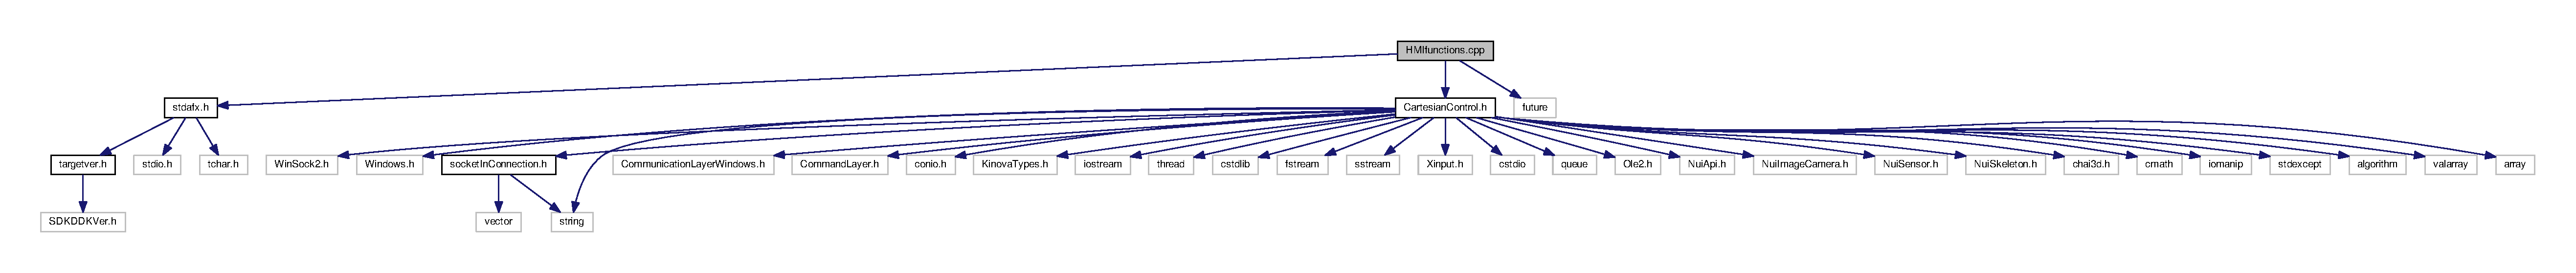
\includegraphics[width=350pt]{d9/d6d/HMIfunctions_8cpp__incl}
\end{center}
\end{figure}
\subsection*{Macros}
\begin{DoxyCompactItemize}
\item 
\#define \hyperlink{HMIfunctions_8cpp_adfc8f90f3a8caa8423099cf36ff214f1}{\+\_\+\+W\+I\+N\+S\+O\+C\+K\+\_\+\+D\+E\+P\+R\+E\+C\+A\+T\+E\+D\+\_\+\+N\+O\+\_\+\+W\+A\+R\+N\+I\+N\+GS}
\end{DoxyCompactItemize}


\subsection{Macro Definition Documentation}
\index{H\+M\+Ifunctions.\+cpp@{H\+M\+Ifunctions.\+cpp}!\+\_\+\+W\+I\+N\+S\+O\+C\+K\+\_\+\+D\+E\+P\+R\+E\+C\+A\+T\+E\+D\+\_\+\+N\+O\+\_\+\+W\+A\+R\+N\+I\+N\+GS@{\+\_\+\+W\+I\+N\+S\+O\+C\+K\+\_\+\+D\+E\+P\+R\+E\+C\+A\+T\+E\+D\+\_\+\+N\+O\+\_\+\+W\+A\+R\+N\+I\+N\+GS}}
\index{\+\_\+\+W\+I\+N\+S\+O\+C\+K\+\_\+\+D\+E\+P\+R\+E\+C\+A\+T\+E\+D\+\_\+\+N\+O\+\_\+\+W\+A\+R\+N\+I\+N\+GS@{\+\_\+\+W\+I\+N\+S\+O\+C\+K\+\_\+\+D\+E\+P\+R\+E\+C\+A\+T\+E\+D\+\_\+\+N\+O\+\_\+\+W\+A\+R\+N\+I\+N\+GS}!H\+M\+Ifunctions.\+cpp@{H\+M\+Ifunctions.\+cpp}}
\subsubsection[{\texorpdfstring{\+\_\+\+W\+I\+N\+S\+O\+C\+K\+\_\+\+D\+E\+P\+R\+E\+C\+A\+T\+E\+D\+\_\+\+N\+O\+\_\+\+W\+A\+R\+N\+I\+N\+GS}{_WINSOCK_DEPRECATED_NO_WARNINGS}}]{\setlength{\rightskip}{0pt plus 5cm}\#define \+\_\+\+W\+I\+N\+S\+O\+C\+K\+\_\+\+D\+E\+P\+R\+E\+C\+A\+T\+E\+D\+\_\+\+N\+O\+\_\+\+W\+A\+R\+N\+I\+N\+GS}\hypertarget{HMIfunctions_8cpp_adfc8f90f3a8caa8423099cf36ff214f1}{}\label{HMIfunctions_8cpp_adfc8f90f3a8caa8423099cf36ff214f1}

\hypertarget{KinovaHMICartesianControl_2HMIfunctions_8cpp}{}\section{H\+M\+Ifunctions.\+cpp File Reference}
\label{KinovaHMICartesianControl_2HMIfunctions_8cpp}\index{H\+M\+Ifunctions.\+cpp@{H\+M\+Ifunctions.\+cpp}}
{\ttfamily \#include \char`\"{}stdafx.\+h\char`\"{}}\\*
{\ttfamily \#include \char`\"{}Cartesian\+Control.\+h\char`\"{}}\\*
{\ttfamily \#include $<$future$>$}\\*
Include dependency graph for Kinova\+H\+M\+I\+Cartesian\+Control/\+H\+M\+Ifunctions.cpp\+:
\nopagebreak
\begin{figure}[H]
\begin{center}
\leavevmode
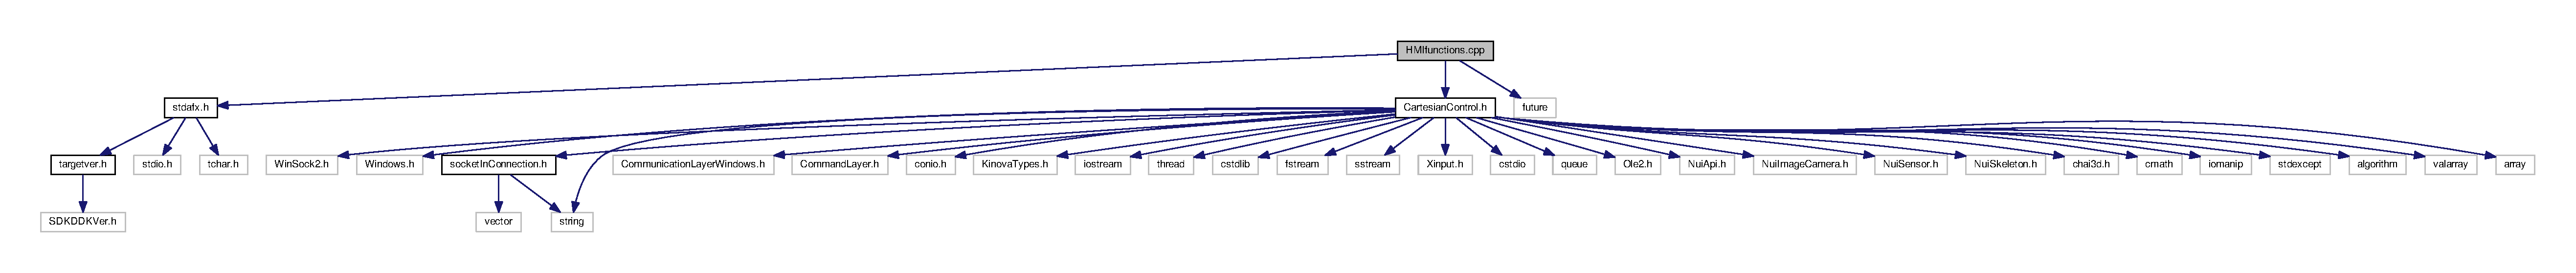
\includegraphics[width=350pt]{d6/dc1/KinovaHMICartesianControl_2HMIfunctions_8cpp__incl}
\end{center}
\end{figure}
\subsection*{Macros}
\begin{DoxyCompactItemize}
\item 
\#define \hyperlink{KinovaHMICartesianControl_2HMIfunctions_8cpp_adfc8f90f3a8caa8423099cf36ff214f1}{\+\_\+\+W\+I\+N\+S\+O\+C\+K\+\_\+\+D\+E\+P\+R\+E\+C\+A\+T\+E\+D\+\_\+\+N\+O\+\_\+\+W\+A\+R\+N\+I\+N\+GS}
\end{DoxyCompactItemize}


\subsection{Macro Definition Documentation}
\index{Kinova\+H\+M\+I\+Cartesian\+Control/\+H\+M\+Ifunctions.\+cpp@{Kinova\+H\+M\+I\+Cartesian\+Control/\+H\+M\+Ifunctions.\+cpp}!\+\_\+\+W\+I\+N\+S\+O\+C\+K\+\_\+\+D\+E\+P\+R\+E\+C\+A\+T\+E\+D\+\_\+\+N\+O\+\_\+\+W\+A\+R\+N\+I\+N\+GS@{\+\_\+\+W\+I\+N\+S\+O\+C\+K\+\_\+\+D\+E\+P\+R\+E\+C\+A\+T\+E\+D\+\_\+\+N\+O\+\_\+\+W\+A\+R\+N\+I\+N\+GS}}
\index{\+\_\+\+W\+I\+N\+S\+O\+C\+K\+\_\+\+D\+E\+P\+R\+E\+C\+A\+T\+E\+D\+\_\+\+N\+O\+\_\+\+W\+A\+R\+N\+I\+N\+GS@{\+\_\+\+W\+I\+N\+S\+O\+C\+K\+\_\+\+D\+E\+P\+R\+E\+C\+A\+T\+E\+D\+\_\+\+N\+O\+\_\+\+W\+A\+R\+N\+I\+N\+GS}!Kinova\+H\+M\+I\+Cartesian\+Control/\+H\+M\+Ifunctions.\+cpp@{Kinova\+H\+M\+I\+Cartesian\+Control/\+H\+M\+Ifunctions.\+cpp}}
\subsubsection[{\texorpdfstring{\+\_\+\+W\+I\+N\+S\+O\+C\+K\+\_\+\+D\+E\+P\+R\+E\+C\+A\+T\+E\+D\+\_\+\+N\+O\+\_\+\+W\+A\+R\+N\+I\+N\+GS}{_WINSOCK_DEPRECATED_NO_WARNINGS}}]{\setlength{\rightskip}{0pt plus 5cm}\#define \+\_\+\+W\+I\+N\+S\+O\+C\+K\+\_\+\+D\+E\+P\+R\+E\+C\+A\+T\+E\+D\+\_\+\+N\+O\+\_\+\+W\+A\+R\+N\+I\+N\+GS}\hypertarget{KinovaHMICartesianControl_2HMIfunctions_8cpp_adfc8f90f3a8caa8423099cf36ff214f1}{}\label{KinovaHMICartesianControl_2HMIfunctions_8cpp_adfc8f90f3a8caa8423099cf36ff214f1}

\hypertarget{jquery_8js}{}\section{jquery.\+js File Reference}
\label{jquery_8js}\index{jquery.\+js@{jquery.\+js}}
\subsection*{Functions}
\begin{DoxyCompactItemize}
\item 
\hyperlink{jquery_8js_a2fa551895933fae935a0a6b87282241d}{b} \hyperlink{jquery_8js_a5fb206c91c64d1be35fde236706eab86}{extend} (\{css\+Hooks\+:\{opacity\+:\{get\+:function(bw, bv)\{\hyperlink{jquery_8js_a42cbfadee2b4749e8f699ea8d745a0e4}{if}(bv)\{var e=\hyperlink{jquery_8js_adc18d83abfd9f87d396e8fd6b6ac0fe1}{Z}(bw,\char`\"{}opacity\char`\"{},\char`\"{}opacity\char`\"{});return e===\char`\"{}\char`\"{}?\char`\"{}1\char`\"{}\+:e\}else\{return bw.\+style.\+opacity\}\}\}\}, css\+Number\+:\{fill\+Opacity\+:true, font\+Weight\+:true, line\+Height\+:true, opacity\+:true, orphans\+:true, widows\+:true, z\+Index\+:true, zoom\+:true\}, css\+Props\+:\{\char`\"{}float\char`\"{}\+:b.\+support.\+css\+Float?\char`\"{}css\+Float\char`\"{}\+:\char`\"{}style\+Float\char`\"{}\}, style\+:function(bx, bw, bD, by)\{\hyperlink{jquery_8js_a42cbfadee2b4749e8f699ea8d745a0e4}{if}(!bx$\vert$$\vert$bx.\+node\+Type===3$\vert$$\vert$bx.\+node\+Type===8$\vert$$\vert$!bx.\+style)\{return\}var bB, bC, bz=b.\+camel\+Case(bw), bv=bx.\+style, bE=b.\+css\+Hooks\mbox{[}bz\mbox{]};bw=b.\+css\+Props\mbox{[}bz\mbox{]}$\vert$$\vert$bz;\hyperlink{jquery_8js_a42cbfadee2b4749e8f699ea8d745a0e4}{if}(b\+D!==\hyperlink{jquery_8js_a38ee4c0b5f4fe2a18d0c783af540d253}{L})\{bC=typeof bD;\hyperlink{jquery_8js_a42cbfadee2b4749e8f699ea8d745a0e4}{if}(bC===\char`\"{}string\char`\"{}\&\&(bB=I.\+exec(bD)))\{bD=(+(bB\mbox{[}1\mbox{]}+1)$\ast$+bB\mbox{[}2\mbox{]})+parse\+Float(\hyperlink{jquery_8js_a89ad527fcd82c01ebb587332f5b4fcd4}{b.\+css}(bx, bw));bC=\char`\"{}number\char`\"{}\}if(bD==null$\vert$$\vert$bC===\char`\"{}number\char`\"{}\&\&is\+NaN(bD))\{return\}\hyperlink{jquery_8js_a42cbfadee2b4749e8f699ea8d745a0e4}{if}(bC===\char`\"{}number\char`\"{}\&\&!b.\+css\+Number\mbox{[}bz\mbox{]})\{bD+=\char`\"{}px\char`\"{}\}if(!bE$\vert$$\vert$!(\char`\"{}set\char`\"{}in bE)$\vert$$\vert$(bD=b\+E.\+set(bx, bD))!==\hyperlink{jquery_8js_a38ee4c0b5f4fe2a18d0c783af540d253}{L})\{try\{bv\mbox{[}bw\mbox{]}=bD\}catch(bA)\{\}\}\}else\{\hyperlink{jquery_8js_a42cbfadee2b4749e8f699ea8d745a0e4}{if}(bE \&\&\char`\"{}get\char`\"{}in bE \&\&(bB=b\+E.\+get(bx, false, by))!==\hyperlink{jquery_8js_a38ee4c0b5f4fe2a18d0c783af540d253}{L})\{return bB\}return bv\mbox{[}bw\mbox{]}\}\}, css\+:function(by, bx, bv)\{var bw, e;bx=b.\+camel\+Case(bx);e=b.\+css\+Hooks\mbox{[}bx\mbox{]};bx=b.\+css\+Props\mbox{[}bx\mbox{]}$\vert$$\vert$bx;\hyperlink{jquery_8js_a42cbfadee2b4749e8f699ea8d745a0e4}{if}(bx===\char`\"{}css\+Float\char`\"{})\{bx=\char`\"{}float\char`\"{}\}if(e \&\&\char`\"{}get\char`\"{}in e \&\&(bw=e.\+get(by, true, bv))!==\hyperlink{jquery_8js_a38ee4c0b5f4fe2a18d0c783af540d253}{L})\{return bw\}else\{\hyperlink{jquery_8js_a42cbfadee2b4749e8f699ea8d745a0e4}{if}(\hyperlink{jquery_8js_adc18d83abfd9f87d396e8fd6b6ac0fe1}{Z})\{return \hyperlink{jquery_8js_adc18d83abfd9f87d396e8fd6b6ac0fe1}{Z}(by, bx)\}\}\}, swap\+:function(bx, bw, by)\{var e=\{\};for(var bv in bw)\{e\mbox{[}bv\mbox{]}=bx.\+style\mbox{[}bv\mbox{]};bx.\+style\mbox{[}bv\mbox{]}=bw\mbox{[}bv\mbox{]}\}by.\+call(bx);for(bv in bw)\{bx.\+style\mbox{[}bv\mbox{]}=e\mbox{[}bv\mbox{]}\}\}\})
\item 
\hyperlink{jquery_8js_a2fa551895933fae935a0a6b87282241d}{b} \hyperlink{jquery_8js_a871ff39db627c54c710a3e9909b8234c}{each} (\mbox{[}\char`\"{}height\char`\"{},\char`\"{}width\char`\"{}\mbox{]}, function(bv, e)\{b.\+css\+Hooks\mbox{[}e\mbox{]}=\{get\+:function(by, bx, bw)\{var bz;\hyperlink{jquery_8js_a42cbfadee2b4749e8f699ea8d745a0e4}{if}(bx)\{\hyperlink{jquery_8js_a42cbfadee2b4749e8f699ea8d745a0e4}{if}(by.\+offset\+Width!==0)\{return \hyperlink{jquery_8js_a2335e57f79b6acfb6de59c235dc8a83e}{p}(by, e, bw)\}else\{b.\+swap(by, a7, function()\{bz=\hyperlink{jquery_8js_a2335e57f79b6acfb6de59c235dc8a83e}{p}(by, e, bw)\})\}return bz\}\}, set\+:function(bw, bx)\{\hyperlink{jquery_8js_a42cbfadee2b4749e8f699ea8d745a0e4}{if}(bc.\+test(bx))\{bx=parse\+Float(bx);\hyperlink{jquery_8js_a42cbfadee2b4749e8f699ea8d745a0e4}{if}(bx $>$=0)\{return bx+\char`\"{}px\char`\"{}\}\}else\{return bx\}\}\}\})
\item 
\hyperlink{jquery_8js_a9db6d45a025ad692282fe23e69eeba43}{if} (!b.\+support.\+opacity)
\item 
\hyperlink{jquery_8js_a2fa551895933fae935a0a6b87282241d}{b} (function()\{\hyperlink{jquery_8js_a42cbfadee2b4749e8f699ea8d745a0e4}{if}(!b.\+support.\+reliable\+Margin\+Right)\{b.\+css\+Hooks.\+margin\+Right=\{get\+:function(bw, bv)\{var e;b.\+swap(bw,\{display\+:\char`\"{}inline-\/block\char`\"{}\}, function()\{\hyperlink{jquery_8js_a42cbfadee2b4749e8f699ea8d745a0e4}{if}(bv)\{e=\hyperlink{jquery_8js_adc18d83abfd9f87d396e8fd6b6ac0fe1}{Z}(bw,\char`\"{}margin-\/right\char`\"{},\char`\"{}margin\+Right\char`\"{})\}else\{e=bw.\+style.\+margin\+Right\}\});return e\}\}\}\})
\item 
\hyperlink{jquery_8js_a30d3d2cd5b567c9f31b2aa30b9cb3bb8}{if} (av.\+default\+View \&\&av.\+default\+View.\+get\+Computed\+Style)
\item 
\hyperlink{jquery_8js_a2c54bd8ed7482e89d19331ba61fe221c}{if} (av.\+document\+Element.\+current\+Style)
\item 
function \hyperlink{jquery_8js_a2335e57f79b6acfb6de59c235dc8a83e}{p} (by, bw, bv)
\item 
\hyperlink{jquery_8js_a42cbfadee2b4749e8f699ea8d745a0e4}{if} (b.\+expr \&\&b.\+expr.\+filters)
\end{DoxyCompactItemize}
\subsection*{Variables}
\begin{DoxyCompactItemize}
\item 
function \hyperlink{jquery_8js_a1d6558865876e1c8cca029fce41a4bdb}{bb}
\item 
function \hyperlink{jquery_8js_a38ee4c0b5f4fe2a18d0c783af540d253}{L} \{var av=bb.\+document,bu=bb.\+navigator,bl=bb.\+location
\item 
var \hyperlink{jquery_8js_aa4026ad5544b958e54ce5e106fa1c805}{b}
\item 
var \hyperlink{jquery_8js_a4fd8ddfab07c8d7c7cae0ab0e052cad3}{au} =/opacity=(\mbox{[}$^\wedge$)\mbox{]}$\ast$)/,z=/(\mbox{[}A-\/\hyperlink{jquery_8js_adc18d83abfd9f87d396e8fd6b6ac0fe1}{Z}\mbox{]}$\vert$$^\wedge$ms)/g,bc=/$^\wedge$-\/?\textbackslash{}d+(?\+:px)?\$/i,bn=/$^\wedge$-\/?\textbackslash{}d/,I=/$^\wedge$(\mbox{[}\textbackslash{}-\/+\mbox{]})=(\mbox{[}\textbackslash{}-\/+.\textbackslash{}de\mbox{]}+)/,a7=\{position\+:\char`\"{}absolute\char`\"{},visibility\+:\char`\"{}hidden\char`\"{},display\+:\char`\"{}block\char`\"{}\},an=\mbox{[}\char`\"{}Left\char`\"{},\char`\"{}Right\char`\"{}\mbox{]},a1=\mbox{[}\char`\"{}Top\char`\"{},\char`\"{}Bottom\char`\"{}\mbox{]},Z,aI,aX
\item 
\hyperlink{jquery_8js_a2fa551895933fae935a0a6b87282241d}{b} fn \hyperlink{jquery_8js_a89ad527fcd82c01ebb587332f5b4fcd4}{css} =function(e,bv)\{\hyperlink{jquery_8js_a42cbfadee2b4749e8f699ea8d745a0e4}{if}(arguments.\+length===2\&\&bv===\hyperlink{jquery_8js_a38ee4c0b5f4fe2a18d0c783af540d253}{L})\{return this\}return b.\+access(this,e,bv,true,function(bx,bw,by)\{return by!==\hyperlink{jquery_8js_a38ee4c0b5f4fe2a18d0c783af540d253}{L}?b.\+style(bx,bw,by)\+:b.\+css(bx,bw)\})\}
\item 
\hyperlink{jquery_8js_a2fa551895933fae935a0a6b87282241d}{b} \hyperlink{jquery_8js_a88b21f8ba3af86d6981b1da520ece33b}{cur\+C\+SS} =\hyperlink{jquery_8js_a89ad527fcd82c01ebb587332f5b4fcd4}{b.\+css}
\item 
\hyperlink{jquery_8js_adc18d83abfd9f87d396e8fd6b6ac0fe1}{Z} =aI$\vert$$\vert$aX
\item 
var \hyperlink{jquery_8js_ab26645c014aa005ecedef329ecf58c99}{k} =/\%20/g
\item 
var \hyperlink{jquery_8js_a6ddf393cc7f9a8828e197bb0d9916c44}{ap} =/\textbackslash{}\mbox{[}\textbackslash{}\mbox{]}\$/
\item 
var \hyperlink{jquery_8js_ae77642f8ef73fb9c20c2a737d956acda}{bs} =/\textbackslash{}r?\textbackslash{}n/g
\item 
var \hyperlink{jquery_8js_af6ee77c71b2c89bdb365145ac5ad1219}{bq} =/\#.$\ast$\$/
\item 
var \hyperlink{jquery_8js_ad223f5fba68c41c1236671ac5c5b0fcb}{aD} =/$^\wedge$(.$\ast$?)\+:\mbox{[} \textbackslash{}t\mbox{]}$\ast$(\mbox{[}$^\wedge$\textbackslash{}r\textbackslash{}n\mbox{]}$\ast$)\textbackslash{}r?\$/mg
\item 
var \hyperlink{jquery_8js_ac87125cdee1a5e57da4ef619af49bc7d}{aZ} =/$^\wedge$(?\+:color$\vert$date$\vert$datetime$\vert$datetime-\/local$\vert$email$\vert$hidden$\vert$month$\vert$number$\vert$password$\vert$range$\vert$search$\vert$tel$\vert$text$\vert$time$\vert$url$\vert$week)\$/i
\item 
var \hyperlink{jquery_8js_a8cc6111a5def3ea889157d13fb9a9672}{aM} =/$^\wedge$(?\+:about$\vert$app$\vert$app\textbackslash{}-\/storage$\vert$.+\textbackslash{}-\/extension$\vert$file$\vert$res$\vert$widget)\+:\$/
\item 
var \hyperlink{jquery_8js_a79eb58dc6cdf0aef563d5dc1ded27df5}{aQ} =/$^\wedge$(?\+:G\+ET$\vert$H\+E\+AD)\$/
\item 
var \hyperlink{jquery_8js_abce695e0af988ece0826d9ad59b8160d}{c}
\end{DoxyCompactItemize}


\subsection{Function Documentation}
\index{jquery.\+js@{jquery.\+js}!b@{b}}
\index{b@{b}!jquery.\+js@{jquery.\+js}}
\subsubsection[{\texorpdfstring{b(function()\lcurly{}if("!b.\+support.\+reliable\+Margin\+Right)\lcurly{}b.\+css\+Hooks.\+margin\+Right=\lcurly{}get\+:function(bw, bv)\lcurly{}var e;b.\+swap(bw,\lcurly{}display\+:""inline-\/block""\rcurly{}, function()\lcurly{}if(bv)\lcurly{}e=\+Z(bw,""margin-\/right"",""margin\+Right"")\rcurly{}else\lcurly{}e=bw.\+style.\+margin\+Right\rcurly{}\rcurly{});return e\rcurly{}\rcurly{}\rcurly{}\rcurly{})}{b(function()\{if(!b.support.reliableMarginRight)\{b.cssHooks.marginRight=\{get:function(bw, bv)\{var e;b.swap(bw,\{display:"inline-block"\}, function()\{if(bv)\{e=Z(bw,"margin-right","marginRight")\}else\{e=bw.style.marginRight\}\});return e\}\}\}\})}}]{\setlength{\rightskip}{0pt plus 5cm}b (
\begin{DoxyParamCaption}
\item[{function()\{{\bf if}(!b.\+support.\+reliable\+Margin\+Right)\{b.\+css\+Hooks.\+margin\+Right=\{get\+:function(bw, bv)\{var e;b.\+swap(bw,\{display\+:\char`\"{}inline-\/block\char`\"{}\}, function()\{{\bf if}(bv)\{e={\bf Z}(bw,\char`\"{}margin-\/right\char`\"{},\char`\"{}margin\+Right\char`\"{})\}else\{e=bw.\+style.\+margin\+Right\}\});return e\}\}\}\}}]{}
\end{DoxyParamCaption}
)}\hypertarget{jquery_8js_a2fa551895933fae935a0a6b87282241d}{}\label{jquery_8js_a2fa551895933fae935a0a6b87282241d}
\index{jquery.\+js@{jquery.\+js}!each@{each}}
\index{each@{each}!jquery.\+js@{jquery.\+js}}
\subsubsection[{\texorpdfstring{each([""height"",""width""], function(bv, e)\lcurly{}b.\+css\+Hooks[e]=\lcurly{}get\+:function(by, bx, bw)\lcurly{}var bz;if(bx)\lcurly{}if(by.\+offset\+Width"!==0)\lcurly{}return p(by, e, bw)\rcurly{}else\lcurly{}b.\+swap(by, a7, function()\lcurly{}bz=p(by, e, bw)\rcurly{})\rcurly{}return bz\rcurly{}\rcurly{}, set\+:function(bw, bx)\lcurly{}if(bc.\+test(bx))\lcurly{}bx=parse\+Float(bx);if(bx $>$=0)\lcurly{}return bx+""px""\rcurly{}\rcurly{}else\lcurly{}return bx\rcurly{}\rcurly{}\rcurly{}\rcurly{})}{each(["height","width"], function(bv, e)\{b.cssHooks[e]=\{get:function(by, bx, bw)\{var bz;if(bx)\{if(by.offsetWidth!==0)\{return p(by, e, bw)\}else\{b.swap(by, a7, function()\{bz=p(by, e, bw)\})\}return bz\}\}, set:function(bw, bx)\{if(bc.test(bx))\{bx=parseFloat(bx);if(bx >=0)\{return bx+"px"\}\}else\{return bx\}\}\}\})}}]{\setlength{\rightskip}{0pt plus 5cm}{\bf b} each (
\begin{DoxyParamCaption}
\item[{function(bv, e)\{b.\+css\+Hooks\mbox{[}e\mbox{]}=\{get\+:function(by, bx, bw)\{var bz;{\bf if}(bx)\{{\bf if}(by.\+offset\+Width!==0)\{return {\bf p}(by, e, bw)\}else\{b.\+swap(by, a7, function()\{bz={\bf p}(by, e, bw)\})\}return bz\}\}, set\+:function(bw, bx)\{{\bf if}(bc.\+test(bx))\{bx=parse\+Float(bx);{\bf if}(bx $>$=0)\{return bx+\char`\"{}px\char`\"{}\}\}else\{return bx\}\}\}\}}]{}
\end{DoxyParamCaption}
)}\hypertarget{jquery_8js_a871ff39db627c54c710a3e9909b8234c}{}\label{jquery_8js_a871ff39db627c54c710a3e9909b8234c}
\index{jquery.\+js@{jquery.\+js}!extend@{extend}}
\index{extend@{extend}!jquery.\+js@{jquery.\+js}}
\subsubsection[{\texorpdfstring{extend(\lcurly{}css\+Hooks\+:\lcurly{}opacity\+:\lcurly{}get\+:function(bw, bv)\lcurly{}if(bv)\lcurly{}var e=\+Z(bw,""opacity"",""opacity"");return e===""""?""1""\+:e\rcurly{}else\lcurly{}return bw.\+style.\+opacity\rcurly{}\rcurly{}\rcurly{}\rcurly{}, css\+Number\+:\lcurly{}fill\+Opacity\+:true, font\+Weight\+:true, line\+Height\+:true, opacity\+:true, orphans\+:true, widows\+:true, z\+Index\+:true, zoom\+:true\rcurly{}, css\+Props\+:\lcurly{}""float""\+:b.\+support.\+css\+Float?""css\+Float""\+:""style\+Float""\rcurly{}, style\+:function(bx, bw, b\+D, by)\lcurly{}if("!bx\texttt{"|}\texttt{"|}bx.\+node\+Type===3\texttt{"|}\texttt{"|}bx.\+node\+Type===8\texttt{"|}\texttt{"|}"!bx.\+style)\lcurly{}return\rcurly{}var b\+B, b\+C, bz=b.\+camel\+Case(bw), bv=bx.\+style, b\+E=b.\+css\+Hooks[bz];bw=b.\+css\+Props[bz]\texttt{"|}\texttt{"|}bz;if(bD"!==\+L)\lcurly{}b\+C=typeof b\+D;if(b\+C===""string""\&\&(b\+B=\+I.\+exec(b\+D)))\lcurly{}b\+D=(+(bB[1]+1)$\ast$+bB[2])+parse\+Float(b.\+css(bx, bw));b\+C=""number""\rcurly{}if(b\+D==null\texttt{"|}\texttt{"|}b\+C===""number""\&\&is\+Na\+N(b\+D))\lcurly{}return\rcurly{}if(b\+C===""number""\&\&"!b.\+css\+Number[bz])\lcurly{}b\+D+=""px""\rcurly{}if("!bE\texttt{"|}\texttt{"|}"!(""set""in b\+E)\texttt{"|}\texttt{"|}(b\+D=b\+E.\+set(bx, b\+D))"!==\+L)\lcurly{}try\lcurly{}bv[bw]=bD\rcurly{}catch(b\+A)\lcurly{}\rcurly{}\rcurly{}\rcurly{}else\lcurly{}if(b\+E \&\&""get""in b\+E \&\&(b\+B=b\+E.\+get(bx, false, by))"!==\+L)\lcurly{}return bB\rcurly{}return bv[bw]\rcurly{}\rcurly{}, css\+:function(by, bx, bv)\lcurly{}var bw, e;bx=b.\+camel\+Case(bx);e=b.\+css\+Hooks[bx];bx=b.\+css\+Props[bx]\texttt{"|}\texttt{"|}bx;if(bx===""css\+Float"")\lcurly{}bx=""float""\rcurly{}if(e \&\&""get""in e \&\&(bw=e.\+get(by, true, bv))"!==\+L)\lcurly{}return bw\rcurly{}else\lcurly{}if(\+Z)\lcurly{}return Z(by, bx)\rcurly{}\rcurly{}\rcurly{}, swap\+:function(bx, bw, by)\lcurly{}var e=\lcurly{}\rcurly{};for(var bv in bw)\lcurly{}e[bv]=bx.\+style[bv];bx.\+style[bv]=bw[bv]\rcurly{}by.\+call(bx);for(bv in bw)\lcurly{}bx.\+style[bv]=e[bv]\rcurly{}\rcurly{}\rcurly{})}{extend(\{cssHooks:\{opacity:\{get:function(bw, bv)\{if(bv)\{var e=Z(bw,"opacity","opacity");return e===""?"1":e\}else\{return bw.style.opacity\}\}\}\}, cssNumber:\{fillOpacity:true, fontWeight:true, lineHeight:true, opacity:true, orphans:true, widows:true, zIndex:true, zoom:true\}, cssProps:\{"float":b.support.cssFloat?"cssFloat":"styleFloat"\}, style:function(bx, bw, bD, by)\{if(!bx||bx.nodeType===3||bx.nodeType===8||!bx.style)\{return\}var bB, bC, bz=b.camelCase(bw), bv=bx.style, bE=b.cssHooks[bz];bw=b.cssProps[bz]||bz;if(bD!==L)\{bC=typeof bD;if(bC==="string"&&(bB=I.exec(bD)))\{bD=(+(bB[1]+1)*+bB[2])+parseFloat(b.css(bx, bw));bC="number"\}if(bD==null||bC==="number"&&isNaN(bD))\{return\}if(bC==="number"&&!b.cssNumber[bz])\{bD+="px"\}if(!bE||!("set"in bE)||(bD=bE.set(bx, bD))!==L)\{try\{bv[bw]=bD\}catch(bA)\{\}\}\}else\{if(bE &&"get"in bE &&(bB=bE.get(bx, false, by))!==L)\{return bB\}return bv[bw]\}\}, css:function(by, bx, bv)\{var bw, e;bx=b.camelCase(bx);e=b.cssHooks[bx];bx=b.cssProps[bx]||bx;if(bx==="cssFloat")\{bx="float"\}if(e &&"get"in e &&(bw=e.get(by, true, bv))!==L)\{return bw\}else\{if(Z)\{return Z(by, bx)\}\}\}, swap:function(bx, bw, by)\{var e=\{\};for(var bv in bw)\{e[bv]=bx.style[bv];bx.style[bv]=bw[bv]\}by.call(bx);for(bv in bw)\{bx.style[bv]=e[bv]\}\}\})}}]{\setlength{\rightskip}{0pt plus 5cm}{\bf b} extend (
\begin{DoxyParamCaption}
\item[{\{css\+Hooks\+:\{opacity\+:\{get\+:function(bw, bv)\{{\bf if}(bv)\{var e={\bf Z}(bw,\char`\"{}opacity\char`\"{},\char`\"{}opacity\char`\"{});return e===\char`\"{}\char`\"{}?\char`\"{}1\char`\"{}\+:e\}else\{return bw.\+style.\+opacity\}\}\}\}, css\+Number\+:\{fill\+Opacity\+:true, font\+Weight\+:true, line\+Height\+:true, opacity\+:true, orphans\+:true, widows\+:true, z\+Index\+:true, zoom\+:true\}, css\+Props\+:\{\char`\"{}float\char`\"{}\+:b.\+support.\+css\+Float?\char`\"{}css\+Float\char`\"{}\+:\char`\"{}style\+Float\char`\"{}\}, style\+:function(bx, bw, bD, by)\{{\bf if}(!bx$\vert$$\vert$bx.\+node\+Type===3$\vert$$\vert$bx.\+node\+Type===8$\vert$$\vert$!bx.\+style)\{return\}var bB, bC, bz=b.\+camel\+Case(bw), bv=bx.\+style, bE=b.\+css\+Hooks\mbox{[}bz\mbox{]};bw=b.\+css\+Props\mbox{[}bz\mbox{]}$\vert$$\vert$bz;{\bf if}(b\+D!=={\bf L})\{bC=typeof bD;{\bf if}(bC===\char`\"{}string\char`\"{}\&\&(bB=I.\+exec(bD)))\{bD=(+(bB\mbox{[}1\mbox{]}+1)$\ast$+bB\mbox{[}2\mbox{]})+parse\+Float({\bf b.\+css}(bx, bw));bC=\char`\"{}number\char`\"{}\}if(bD==null$\vert$$\vert$bC===\char`\"{}number\char`\"{}\&\&is\+NaN(bD))\{return\}{\bf if}(bC===\char`\"{}number\char`\"{}\&\&!b.\+css\+Number\mbox{[}bz\mbox{]})\{bD+=\char`\"{}px\char`\"{}\}if(!bE$\vert$$\vert$!(\char`\"{}set\char`\"{}in bE)$\vert$$\vert$(bD=b\+E.\+set(bx, bD))!=={\bf L})\{try\{bv\mbox{[}bw\mbox{]}=bD\}catch(bA)\{\}\}\}else\{{\bf if}(bE \&\&\char`\"{}get\char`\"{}in bE \&\&(bB=b\+E.\+get(bx, false, by))!=={\bf L})\{return bB\}return bv\mbox{[}bw\mbox{]}\}\}, css\+:function(by, bx, bv)\{var bw, e;bx=b.\+camel\+Case(bx);e=b.\+css\+Hooks\mbox{[}bx\mbox{]};bx=b.\+css\+Props\mbox{[}bx\mbox{]}$\vert$$\vert$bx;{\bf if}(bx===\char`\"{}css\+Float\char`\"{})\{bx=\char`\"{}float\char`\"{}\}if(e \&\&\char`\"{}get\char`\"{}in e \&\&(bw=e.\+get(by, true, bv))!=={\bf L})\{return bw\}else\{{\bf if}({\bf Z})\{return {\bf Z}(by, bx)\}\}\}, swap\+:function(bx, bw, by)\{var e=\{\};for(var bv in bw)\{e\mbox{[}bv\mbox{]}=bx.\+style\mbox{[}bv\mbox{]};bx.\+style\mbox{[}bv\mbox{]}=bw\mbox{[}bv\mbox{]}\}by.\+call(bx);for(bv in bw)\{bx.\+style\mbox{[}bv\mbox{]}=e\mbox{[}bv\mbox{]}\}\}\}}]{}
\end{DoxyParamCaption}
)}\hypertarget{jquery_8js_a5fb206c91c64d1be35fde236706eab86}{}\label{jquery_8js_a5fb206c91c64d1be35fde236706eab86}
\index{jquery.\+js@{jquery.\+js}!if@{if}}
\index{if@{if}!jquery.\+js@{jquery.\+js}}
\subsubsection[{\texorpdfstring{if(av.\+document\+Element.\+current\+Style)}{if(av.documentElement.currentStyle)}}]{\setlength{\rightskip}{0pt plus 5cm}if (
\begin{DoxyParamCaption}
\item[{av.\+document\+Element.}]{current\+Style}
\end{DoxyParamCaption}
)}\hypertarget{jquery_8js_a2c54bd8ed7482e89d19331ba61fe221c}{}\label{jquery_8js_a2c54bd8ed7482e89d19331ba61fe221c}
\index{jquery.\+js@{jquery.\+js}!if@{if}}
\index{if@{if}!jquery.\+js@{jquery.\+js}}
\subsubsection[{\texorpdfstring{if(av.\+default\+View \&\&av.\+default\+View.\+get\+Computed\+Style)}{if(av.defaultView &&av.defaultView.getComputedStyle)}}]{\setlength{\rightskip}{0pt plus 5cm}if (
\begin{DoxyParamCaption}
\item[{av.\+default\+View \&\&av.\+default\+View.}]{get\+Computed\+Style}
\end{DoxyParamCaption}
)}\hypertarget{jquery_8js_a30d3d2cd5b567c9f31b2aa30b9cb3bb8}{}\label{jquery_8js_a30d3d2cd5b567c9f31b2aa30b9cb3bb8}
\index{jquery.\+js@{jquery.\+js}!if@{if}}
\index{if@{if}!jquery.\+js@{jquery.\+js}}
\subsubsection[{\texorpdfstring{if(b.\+expr \&\&b.\+expr.\+filters)}{if(b.expr &&b.expr.filters)}}]{\setlength{\rightskip}{0pt plus 5cm}if (
\begin{DoxyParamCaption}
\item[{b.\+expr \&\&b.\+expr.}]{filters}
\end{DoxyParamCaption}
)}\hypertarget{jquery_8js_a42cbfadee2b4749e8f699ea8d745a0e4}{}\label{jquery_8js_a42cbfadee2b4749e8f699ea8d745a0e4}
\index{jquery.\+js@{jquery.\+js}!if@{if}}
\index{if@{if}!jquery.\+js@{jquery.\+js}}
\subsubsection[{\texorpdfstring{if("!b.\+support.\+opacity)}{if(!b.support.opacity)}}]{\setlength{\rightskip}{0pt plus 5cm}if (
\begin{DoxyParamCaption}
\item[{!b.\+support.}]{opacity}
\end{DoxyParamCaption}
)}\hypertarget{jquery_8js_a9db6d45a025ad692282fe23e69eeba43}{}\label{jquery_8js_a9db6d45a025ad692282fe23e69eeba43}
\index{jquery.\+js@{jquery.\+js}!p@{p}}
\index{p@{p}!jquery.\+js@{jquery.\+js}}
\subsubsection[{\texorpdfstring{p(by, bw, bv)}{p(by, bw, bv)}}]{\setlength{\rightskip}{0pt plus 5cm}function p (
\begin{DoxyParamCaption}
\item[{}]{by, }
\item[{}]{bw, }
\item[{}]{bv}
\end{DoxyParamCaption}
)}\hypertarget{jquery_8js_a2335e57f79b6acfb6de59c235dc8a83e}{}\label{jquery_8js_a2335e57f79b6acfb6de59c235dc8a83e}


\subsection{Variable Documentation}
\index{jquery.\+js@{jquery.\+js}!aD@{aD}}
\index{aD@{aD}!jquery.\+js@{jquery.\+js}}
\subsubsection[{\texorpdfstring{aD}{aD}}]{\setlength{\rightskip}{0pt plus 5cm}var aD =/$^\wedge$(.$\ast$?)\+:\mbox{[} \textbackslash{}t\mbox{]}$\ast$(\mbox{[}$^\wedge$\textbackslash{}r\textbackslash{}n\mbox{]}$\ast$)\textbackslash{}r?\$/mg}\hypertarget{jquery_8js_ad223f5fba68c41c1236671ac5c5b0fcb}{}\label{jquery_8js_ad223f5fba68c41c1236671ac5c5b0fcb}
\index{jquery.\+js@{jquery.\+js}!aM@{aM}}
\index{aM@{aM}!jquery.\+js@{jquery.\+js}}
\subsubsection[{\texorpdfstring{aM}{aM}}]{\setlength{\rightskip}{0pt plus 5cm}var aM =/$^\wedge$(?\+:about$\vert$app$\vert$app\textbackslash{}-\/storage$\vert$.+\textbackslash{}-\/extension$\vert$file$\vert$res$\vert$widget)\+:\$/}\hypertarget{jquery_8js_a8cc6111a5def3ea889157d13fb9a9672}{}\label{jquery_8js_a8cc6111a5def3ea889157d13fb9a9672}
\index{jquery.\+js@{jquery.\+js}!ap@{ap}}
\index{ap@{ap}!jquery.\+js@{jquery.\+js}}
\subsubsection[{\texorpdfstring{ap}{ap}}]{\setlength{\rightskip}{0pt plus 5cm}var ap =/\textbackslash{}\mbox{[}\textbackslash{}\mbox{]}\$/}\hypertarget{jquery_8js_a6ddf393cc7f9a8828e197bb0d9916c44}{}\label{jquery_8js_a6ddf393cc7f9a8828e197bb0d9916c44}
\index{jquery.\+js@{jquery.\+js}!aQ@{aQ}}
\index{aQ@{aQ}!jquery.\+js@{jquery.\+js}}
\subsubsection[{\texorpdfstring{aQ}{aQ}}]{\setlength{\rightskip}{0pt plus 5cm}var aQ =/$^\wedge$(?\+:G\+ET$\vert$H\+E\+AD)\$/}\hypertarget{jquery_8js_a79eb58dc6cdf0aef563d5dc1ded27df5}{}\label{jquery_8js_a79eb58dc6cdf0aef563d5dc1ded27df5}
\index{jquery.\+js@{jquery.\+js}!au@{au}}
\index{au@{au}!jquery.\+js@{jquery.\+js}}
\subsubsection[{\texorpdfstring{au}{au}}]{\setlength{\rightskip}{0pt plus 5cm}var au =/opacity=(\mbox{[}$^\wedge$)\mbox{]}$\ast$)/,z=/(\mbox{[}A-\/{\bf Z}\mbox{]}$\vert$$^\wedge$ms)/g,bc=/$^\wedge$-\/?\textbackslash{}d+(?\+:px)?\$/i,bn=/$^\wedge$-\/?\textbackslash{}d/,I=/$^\wedge$(\mbox{[}\textbackslash{}-\/+\mbox{]})=(\mbox{[}\textbackslash{}-\/+.\textbackslash{}de\mbox{]}+)/,a7=\{position\+:\char`\"{}absolute\char`\"{},visibility\+:\char`\"{}hidden\char`\"{},display\+:\char`\"{}block\char`\"{}\},an=\mbox{[}\char`\"{}Left\char`\"{},\char`\"{}Right\char`\"{}\mbox{]},a1=\mbox{[}\char`\"{}Top\char`\"{},\char`\"{}Bottom\char`\"{}\mbox{]},Z,aI,aX}\hypertarget{jquery_8js_a4fd8ddfab07c8d7c7cae0ab0e052cad3}{}\label{jquery_8js_a4fd8ddfab07c8d7c7cae0ab0e052cad3}
\index{jquery.\+js@{jquery.\+js}!aZ@{aZ}}
\index{aZ@{aZ}!jquery.\+js@{jquery.\+js}}
\subsubsection[{\texorpdfstring{aZ}{aZ}}]{\setlength{\rightskip}{0pt plus 5cm}var aZ =/$^\wedge$(?\+:color$\vert$date$\vert$datetime$\vert$datetime-\/local$\vert$email$\vert$hidden$\vert$month$\vert$number$\vert$password$\vert$range$\vert$search$\vert$tel$\vert$text$\vert$time$\vert$url$\vert$week)\$/i}\hypertarget{jquery_8js_ac87125cdee1a5e57da4ef619af49bc7d}{}\label{jquery_8js_ac87125cdee1a5e57da4ef619af49bc7d}
\index{jquery.\+js@{jquery.\+js}!b@{b}}
\index{b@{b}!jquery.\+js@{jquery.\+js}}
\subsubsection[{\texorpdfstring{b}{b}}]{\setlength{\rightskip}{0pt plus 5cm}var b}\hypertarget{jquery_8js_aa4026ad5544b958e54ce5e106fa1c805}{}\label{jquery_8js_aa4026ad5544b958e54ce5e106fa1c805}
{\bfseries Initial value\+:}
\begin{DoxyCode}
=(\textcolor{keyword}{function}()\{var bF=\textcolor{keyword}{function}(b0,b1)\{\textcolor{keywordflow}{return} \textcolor{keyword}{new} bF.fn.init(b0,b1,bD)\},bU=\hyperlink{jquery_8js_a1d6558865876e1c8cca029fce41a4bdb}{bb}.jQuery,bH=
      \hyperlink{jquery_8js_a1d6558865876e1c8cca029fce41a4bdb}{bb}.$,bD,bY=/^(?:[^#<]*(<[\(\backslash\)w\(\backslash\)W]+>)[^>]*$|#([\(\backslash\)w\(\backslash\)-]*)$)/,bM=/\(\backslash\)S/,bI=/^\(\backslash\)s+/,bE=/\(\backslash\)s+$/,bA=/^<(\(\backslash\)w+)\(\backslash\)s*\(\backslash\)/?>(?:<\(\backslash\)
      /\(\backslash\)1>)?$/,bN=/^[\(\backslash\)],:\{\}\(\backslash\)s]*$/,bW=/\(\backslash\)\(\backslash\)(?:[\textcolor{stringliteral}{"\(\backslash\)\(\backslash\)\(\backslash\)/bfnrt]|u[0-9a-fA-F]\{4\})/g,bP=/"}[^\textcolor{stringliteral}{"\(\backslash\)\(\backslash\)\(\backslash\)n\(\backslash\)r]*"}|\textcolor{keyword}{true}|\textcolor{keyword}{false}|null|-?\(\backslash\)d+
      (?:\(\backslash\).\(\backslash\)d*)?(?:[eE][+\(\backslash\)-]?\(\backslash\)d+)?/g,bJ=/(?:^|:|,)(?:\(\backslash\)s*\(\backslash\)[)+/g,by=/(webkit)[ \(\backslash\)/]([\(\backslash\)w.]+)/,bR=/(opera)(?:.*version)
      ?[ \(\backslash\)/]([\(\backslash\)w.]+)/,bQ=/(msie) ([\(\backslash\)w.]+)/,bS=/(mozilla)(?:.*? rv:([\(\backslash\)w.]+))?/,bB=/-([a-z]|[0-9])/ig,bZ=/^-ms-/,bT=\textcolor{keyword}{
      function}(b0,b1)\{\textcolor{keywordflow}{return}(b1+\textcolor{stringliteral}{""}).toUpperCase()\},bX=bu.userAgent,bV,bC,e,bL=Object.prototype.toString,bG=Object.
      prototype.hasOwnProperty,bz=Array.prototype.push,bK=Array.prototype.slice,bO=String.prototype.trim,bv=Array.
      prototype.indexOf,bx=\{\};bF.fn=bF.prototype=\{constructor:bF,init:\textcolor{keyword}{function}(b0,b4,b3)\{var b2,b5,b1,b6;\textcolor{keywordflow}{if}(!b0)\{\textcolor{keywordflow}{
      return} \textcolor{keyword}{this}\}\textcolor{keywordflow}{if}(b0.nodeType)\{this.context=\textcolor{keyword}{this}[0]=b0;this.length=1;\textcolor{keywordflow}{return} \textcolor{keyword}{this}\}\textcolor{keywordflow}{if}(b0===\textcolor{stringliteral}{"body"}&&!b4&&av.body)\{
      this.context=av;\textcolor{keyword}{this}[0]=av.body;this.selector=b0;this.length=1;\textcolor{keywordflow}{return} \textcolor{keyword}{this}\}\textcolor{keywordflow}{if}(typeof b0===\textcolor{stringliteral}{"string"})\{\textcolor{keywordflow}{if}(b0.
      charAt(0)===\textcolor{stringliteral}{"<"}&&b0.charAt(b0.length-1)===\textcolor{stringliteral}{">"}&&b0.length>=3)\{b2=[null,b0,null]\}\textcolor{keywordflow}{else}\{b2=bY.exec(b0)\}\textcolor{keywordflow}{if}(b2&&(b2[1
      ]||!b4))\{\textcolor{keywordflow}{if}(b2[1])\{b4=b4 instanceof bF?b4[0]:b4;b6=(b4?b4.ownerDocument||b4:av);b1=bA.exec(b0);\textcolor{keywordflow}{if}(b1)\{\textcolor{keywordflow}{if}(bF.
      isPlainObject(b4))\{b0=[av.createElement(b1[1])];bF.fn.attr.call(b0,b4,\textcolor{keyword}{true})\}\textcolor{keywordflow}{else}\{b0=[b6.createElement(b1[1])
      ]\}\}\textcolor{keywordflow}{else}\{b1=bF.buildFragment([b2[1]],[b6]);b0=(b1.cacheable?bF.clone(b1.fragment):b1.fragment).childNodes\}\textcolor{keywordflow}{
      return} bF.merge(\textcolor{keyword}{this},b0)\}\textcolor{keywordflow}{else}\{b5=av.getElementById(b2[2]);\textcolor{keywordflow}{if}(b5&&b5.parentNode)\{\textcolor{keywordflow}{if}(b5.id!==b2[2])\{\textcolor{keywordflow}{return} b3.
      find(b0)\}this.length=1;\textcolor{keyword}{this}[0]=b5\}this.context=av;this.selector=b0;\textcolor{keywordflow}{return} \textcolor{keyword}{this}\}\}\textcolor{keywordflow}{else}\{\textcolor{keywordflow}{if}(!b4||b4.jquery)\{\textcolor{keywordflow}{return}(
      b4||b3).find(b0)\}\textcolor{keywordflow}{else}\{\textcolor{keywordflow}{return} this.constructor(b4).find(b0)\}\}\}\textcolor{keywordflow}{else}\{\textcolor{keywordflow}{if}(bF.isFunction(b0))\{\textcolor{keywordflow}{return} b3.ready(b0)\}
      \}\textcolor{keywordflow}{if}(b0.selector!==\hyperlink{jquery_8js_a38ee4c0b5f4fe2a18d0c783af540d253}{L})\{this.selector=b0.selector;this.context=b0.context\}\textcolor{keywordflow}{return} bF.makeArray(b0,\textcolor{keyword}{this})\},
      selector:\textcolor{stringliteral}{""},jquery:\textcolor{stringliteral}{"1.7.1"},length:0,size:\textcolor{keyword}{function}()\{\textcolor{keywordflow}{return} this.length\},toArray:\textcolor{keyword}{function}()\{\textcolor{keywordflow}{return} bK.call(\textcolor{keyword}{this},0)\}
      ,\textcolor{keyword}{get}:\textcolor{keyword}{function}(b0)\{\textcolor{keywordflow}{return} b0==null?this.toArray():(b0<0?this[this.length+b0]:this[b0])\},pushStack:function(b1
      ,b3,b0)\{var b2=this.constructor();\textcolor{keywordflow}{if}(bF.isArray(b1))\{bz.apply(b2,b1)\}\textcolor{keywordflow}{else}\{bF.merge(b2,b1)\}b2.prevObject=\textcolor{keyword}{this}
      ;b2.context=this.context;\textcolor{keywordflow}{if}(b3===\textcolor{stringliteral}{"find"})\{b2.selector=this.selector+(this.selector?\textcolor{stringliteral}{" "}:\textcolor{stringliteral}{""})+b0\}\textcolor{keywordflow}{else}\{\textcolor{keywordflow}{if}(b3)\{b2.
      selector=this.selector+\textcolor{stringliteral}{"."}+b3+\textcolor{stringliteral}{"("}+b0+\textcolor{stringliteral}{")"}\}\}\textcolor{keywordflow}{return} b2\},\hyperlink{jquery_8js_a871ff39db627c54c710a3e9909b8234c}{each}:\textcolor{keyword}{function}(b1,b0)\{\textcolor{keywordflow}{return} bF.each(\textcolor{keyword}{this},b1,b0)\},
      ready:\textcolor{keyword}{function}(b0)\{bF.bindReady();bC.add(b0);\textcolor{keywordflow}{return} \textcolor{keyword}{this}\},eq:\textcolor{keyword}{function}(b0)\{b0=+b0;\textcolor{keywordflow}{return} b0===-1?this.slice(b0)
      :this.slice(b0,b0+1)\},first:function()\{\textcolor{keywordflow}{return} this.eq(0)\},last:\textcolor{keyword}{function}()\{\textcolor{keywordflow}{return} this.eq(-1)\},slice:\textcolor{keyword}{function}
      ()\{\textcolor{keywordflow}{return} this.pushStack(bK.apply(\textcolor{keyword}{this},arguments),\textcolor{stringliteral}{"slice"},bK.call(arguments).join(\textcolor{stringliteral}{","}))\},map:\textcolor{keyword}{function}(b0)\{\textcolor{keywordflow}{
      return} this.pushStack(bF.map(\textcolor{keyword}{this},\textcolor{keyword}{function}(b2,b1)\{return b0.call(b2,b1,b2)\}))\},end:\textcolor{keyword}{function}()\{\textcolor{keywordflow}{return} this.
      prevObject||this.constructor(null)\},push:bz,sort:[].sort,splice:[].splice\};bF.fn.init.prototype=bF.fn;bF.extend=
      bF.fn.extend=\textcolor{keyword}{function}()\{var b9,b2,b0,b1,b6,b7,b5=arguments[0]||\{\},b4=1,b3=arguments.length,b8=\textcolor{keyword}{false};\textcolor{keywordflow}{if}(
      typeof b5===\textcolor{stringliteral}{"boolean"})\{b8=b5;b5=arguments[1]||\{\};b4=2\}\textcolor{keywordflow}{if}(typeof b5!==\textcolor{stringliteral}{"object"}&&!bF.isFunction(b5))\{b5=\{\}\}\textcolor{keywordflow}{if}(b3===
      b4)\{b5=\textcolor{keyword}{this};--b4\}\textcolor{keywordflow}{for}(;b4<b3;b4++)\{\textcolor{keywordflow}{if}((b9=arguments[b4])!=null)\{\textcolor{keywordflow}{for}(b2 in b9)\{b0=b5[b2];b1=b9[b2];\textcolor{keywordflow}{if}(b5===b1)
      \{\textcolor{keywordflow}{continue}\}\textcolor{keywordflow}{if}(b8&&b1&&(bF.isPlainObject(b1)||(b6=bF.isArray(b1))))\{\textcolor{keywordflow}{if}(b6)\{b6=\textcolor{keyword}{false};b7=b0&&bF.isArray(b0)?b0:[
      ]\}\textcolor{keywordflow}{else}\{b7=b0&&bF.isPlainObject(b0)?b0:\{\}\}b5[b2]=bF.extend(b8,b7,b1)\}\textcolor{keywordflow}{else}\{\textcolor{keywordflow}{if}(b1!==
      \hyperlink{jquery_8js_a38ee4c0b5f4fe2a18d0c783af540d253}{L})\{b5[b2]=b1\}\}\}\}\}\textcolor{keywordflow}{return} b5\};bF.extend(\{noConflict:\textcolor{keyword}{function}(b0)\{\textcolor{keywordflow}{if}(\hyperlink{jquery_8js_a1d6558865876e1c8cca029fce41a4bdb}{bb}.$===bF)\{
      \hyperlink{jquery_8js_a1d6558865876e1c8cca029fce41a4bdb}{bb}.$=bH\}\textcolor{keywordflow}{if}(b0&&\hyperlink{jquery_8js_a1d6558865876e1c8cca029fce41a4bdb}{bb}.jQuery===bF)\{\hyperlink{jquery_8js_a1d6558865876e1c8cca029fce41a4bdb}{bb}.jQuery=bU\}\textcolor{keywordflow}{return} bF\},isReady:\textcolor{keyword}{false},readyWait:1,holdReady:\textcolor{keyword}{function}(
      b0)\{\textcolor{keywordflow}{if}(b0)\{bF.readyWait++\}\textcolor{keywordflow}{else}\{bF.ready(\textcolor{keyword}{true})\}\},ready:\textcolor{keyword}{function}(b0)\{\textcolor{keywordflow}{if}((b0===\textcolor{keyword}{true}&&!--bF.readyWait)||(b0!==\textcolor{keyword}{
      true}&&!bF.isReady))\{\textcolor{keywordflow}{if}(!av.body)\{\textcolor{keywordflow}{return} setTimeout(bF.ready,1)\}bF.isReady=\textcolor{keyword}{true};\textcolor{keywordflow}{if}(b0!==\textcolor{keyword}{true}&&--bF.readyWait>0)\{\textcolor{keywordflow}{
      return}\}bC.fireWith(av,[bF]);\textcolor{keywordflow}{if}(bF.fn.trigger)\{bF(av).trigger(\textcolor{stringliteral}{"ready"}).off(\textcolor{stringliteral}{"ready"})\}\}\},bindReady:\textcolor{keyword}{function}()\{\textcolor{keywordflow}{
      if}(bC)\{\textcolor{keywordflow}{return}\}bC=bF.Callbacks(\textcolor{stringliteral}{"once memory"});\textcolor{keywordflow}{if}(av.readyState===\textcolor{stringliteral}{"complete"})\{\textcolor{keywordflow}{return} setTimeout(bF.ready,1)\}\textcolor{keywordflow}{if}(
      av.addEventListener)\{av.addEventListener(\textcolor{stringliteral}{"DOMContentLoaded"},e,\textcolor{keyword}{false});\hyperlink{jquery_8js_a1d6558865876e1c8cca029fce41a4bdb}{bb}.addEventListener(\textcolor{stringliteral}{"load"},bF.ready,\textcolor{keyword}{
      false})\}\textcolor{keywordflow}{else}\{\textcolor{keywordflow}{if}(av.attachEvent)\{av.attachEvent(\textcolor{stringliteral}{"onreadystatechange"},e);\hyperlink{jquery_8js_a1d6558865876e1c8cca029fce41a4bdb}{bb}.attachEvent(\textcolor{stringliteral}{"onload"},bF.ready);var
       b0=\textcolor{keyword}{false};\textcolor{keywordflow}{try}\{b0=\hyperlink{jquery_8js_a1d6558865876e1c8cca029fce41a4bdb}{bb}.frameElement==null\}\textcolor{keywordflow}{catch}(b1)\{\}\textcolor{keywordflow}{if}(av.documentElement.doScroll&&b0)\{bw()\}\}\}\},isFunction:\textcolor{keyword}{
      function}(b0)\{\textcolor{keywordflow}{return} bF.type(b0)===\textcolor{stringliteral}{"function"}\},isArray:Array.isArray||\textcolor{keyword}{function}(b0)\{\textcolor{keywordflow}{return} bF.type(b0)===\textcolor{stringliteral}{"
      array"}\},isWindow:\textcolor{keyword}{function}(b0)\{\textcolor{keywordflow}{return} b0&&typeof b0===\textcolor{stringliteral}{"object"}&&\textcolor{stringliteral}{"setInterval"} in b0\},isNumeric:\textcolor{keyword}{function}(b0)\{\textcolor{keywordflow}{
      return} !isNaN(parseFloat(b0))&&isFinite(b0)\},type:\textcolor{keyword}{function}(b0)\{\textcolor{keywordflow}{return} b0==null?String(b0):bx[bL.call(b0)]||\textcolor{stringliteral}{"
      object"}\},isPlainObject:function(b2)\{\textcolor{keywordflow}{if}(!b2||bF.type(b2)!==\textcolor{stringliteral}{"object"}||b2.nodeType||bF.isWindow(b2))\{\textcolor{keywordflow}{return} \textcolor{keyword}{false}\}\textcolor{keywordflow}{
      try}\{\textcolor{keywordflow}{if}(b2.constructor&&!bG.call(b2,\textcolor{stringliteral}{"constructor"})&&!bG.call(b2.constructor.prototype,\textcolor{stringliteral}{"isPrototypeOf"}))\{\textcolor{keywordflow}{return} \textcolor{keyword}{
      false}\}\}\textcolor{keywordflow}{catch}(b1)\{\textcolor{keywordflow}{return} \textcolor{keyword}{false}\}var b0;\textcolor{keywordflow}{for}(b0 in b2)\{\}\textcolor{keywordflow}{return} b0===\hyperlink{jquery_8js_a38ee4c0b5f4fe2a18d0c783af540d253}{L}||bG.call(b2,b0)\},isEmptyObject:\textcolor{keyword}{function}(
      b1)\{\textcolor{keywordflow}{for}(var b0 in b1)\{\textcolor{keywordflow}{return} \textcolor{keyword}{false}\}\textcolor{keywordflow}{return} \textcolor{keyword}{true}\},error:\textcolor{keyword}{function}(b0)\{\textcolor{keywordflow}{throw} \textcolor{keyword}{new} Error(b0)\},parseJSON:\textcolor{keyword}{function}(b0
      )\{\textcolor{keywordflow}{if}(typeof b0!==\textcolor{stringliteral}{"string"}||!b0)\{\textcolor{keywordflow}{return} null\}b0=bF.trim(b0);\textcolor{keywordflow}{if}(\hyperlink{jquery_8js_a1d6558865876e1c8cca029fce41a4bdb}{bb}.JSON&&\hyperlink{jquery_8js_a1d6558865876e1c8cca029fce41a4bdb}{bb}.JSON.parse)\{\textcolor{keywordflow}{return} 
      \hyperlink{jquery_8js_a1d6558865876e1c8cca029fce41a4bdb}{bb}.JSON.parse(b0)\}\textcolor{keywordflow}{if}(bN.test(b0.replace(bW,\textcolor{stringliteral}{"@"}).replace(bP,\textcolor{stringliteral}{"]"}).replace(bJ,\textcolor{stringliteral}{""})))\{\textcolor{keywordflow}{return}(\textcolor{keyword}{new} Function(\textcolor{stringliteral}{"
      return "}+b0))()\}bF.error(\textcolor{stringliteral}{"Invalid JSON: "}+b0)\},parseXML:\textcolor{keyword}{function}(b2)\{var b0,b1;\textcolor{keywordflow}{try}\{\textcolor{keywordflow}{if}(
      \hyperlink{jquery_8js_a1d6558865876e1c8cca029fce41a4bdb}{bb}.DOMParser)\{b1=\textcolor{keyword}{new} DOMParser();b0=b1.parseFromString(b2,\textcolor{stringliteral}{"text/xml"})\}\textcolor{keywordflow}{else}\{b0=\textcolor{keyword}{new} ActiveXObject(\textcolor{stringliteral}{"
      Microsoft.XMLDOM"});b0.async=\textcolor{stringliteral}{"false"};b0.loadXML(b2)\}\}\textcolor{keywordflow}{catch}(b3)\{b0=\hyperlink{jquery_8js_a38ee4c0b5f4fe2a18d0c783af540d253}{L}\}\textcolor{keywordflow}{if}(!b0||!b0.documentElement||b0.
      getElementsByTagName(\textcolor{stringliteral}{"parsererror"}).length)\{bF.error(\textcolor{stringliteral}{"Invalid XML: "}+b2)\}\textcolor{keywordflow}{return} b0\},noop:\textcolor{keyword}{function}()\{\},globalEval:\textcolor{keyword}{function}(b0
      )\{\textcolor{keywordflow}{if}(b0&&bM.test(b0))\{(\hyperlink{jquery_8js_a1d6558865876e1c8cca029fce41a4bdb}{bb}.execScript||\textcolor{keyword}{function}(b1)\{\hyperlink{jquery_8js_a1d6558865876e1c8cca029fce41a4bdb}{bb}[\textcolor{stringliteral}{"eval"}].call(\hyperlink{jquery_8js_a1d6558865876e1c8cca029fce41a4bdb}{bb},b1)\})(b0)\}\},camelCase:\textcolor{keyword}{function}(
      b0)\{\textcolor{keywordflow}{return} b0.replace(bZ,\textcolor{stringliteral}{"ms-"}).replace(bB,bT)\},nodeName:\textcolor{keyword}{function}(b1,b0)\{\textcolor{keywordflow}{return} b1.nodeName&&b1.nodeName.
      toUpperCase()===b0.toUpperCase()\},\hyperlink{jquery_8js_a871ff39db627c54c710a3e9909b8234c}{each}:\textcolor{keyword}{function}(b3,b6,b2)\{var b1,b4=0,b5=b3.length,b0=b5===
      \hyperlink{jquery_8js_a38ee4c0b5f4fe2a18d0c783af540d253}{L}||bF.isFunction(b3);\textcolor{keywordflow}{if}(b2)\{\textcolor{keywordflow}{if}(b0)\{\textcolor{keywordflow}{for}(b1 in b3)\{\textcolor{keywordflow}{if}(b6.apply(b3[b1],b2)===\textcolor{keyword}{false})\{\textcolor{keywordflow}{break}\}\}\}\textcolor{keywordflow}{else}\{\textcolor{keywordflow}{for}(;b4<b5;)
      \{\textcolor{keywordflow}{if}(b6.apply(b3[b4++],b2)===\textcolor{keyword}{false})\{\textcolor{keywordflow}{break}\}\}\}\}\textcolor{keywordflow}{else}\{\textcolor{keywordflow}{if}(b0)\{\textcolor{keywordflow}{for}(b1 in b3)\{\textcolor{keywordflow}{if}(b6.call(b3[b1],b1,b3[b1])===\textcolor{keyword}{false})\{\textcolor{keywordflow}{
      break}\}\}\}\textcolor{keywordflow}{else}\{\textcolor{keywordflow}{for}(;b4<b5;)\{\textcolor{keywordflow}{if}(b6.call(b3[b4],b4,b3[b4++])===\textcolor{keyword}{false})\{\textcolor{keywordflow}{break}\}\}\}\}\textcolor{keywordflow}{return} b3\},trim:bO?\textcolor{keyword}{function}(b0)\{\textcolor{keywordflow}{
      return} b0==null?\textcolor{stringliteral}{""}:bO.call(b0)\}:\textcolor{keyword}{function}(b0)\{\textcolor{keywordflow}{return} b0==null?\textcolor{stringliteral}{""}:b0.toString().replace(bI,\textcolor{stringliteral}{""}).replace(bE,\textcolor{stringliteral}{""})\},
      makeArray:\textcolor{keyword}{function}(b3,b1)\{var b0=b1||[];\textcolor{keywordflow}{if}(b3!=null)\{var b2=bF.type(b3);\textcolor{keywordflow}{if}(b3.length==null||b2===\textcolor{stringliteral}{"string"}||
      b2===\textcolor{stringliteral}{"function"}||b2===\textcolor{stringliteral}{"regexp"}||bF.isWindow(b3))\{bz.call(b0,b3)\}\textcolor{keywordflow}{else}\{bF.merge(b0,b3)\}\}\textcolor{keywordflow}{return} b0\},inArray:\textcolor{keyword}{
      function}(b2,b3,b1)\{var b0;\textcolor{keywordflow}{if}(b3)\{\textcolor{keywordflow}{if}(bv)\{\textcolor{keywordflow}{return} bv.call(b3,b2,b1)\}b0=b3.length;b1=b1?b1<0?Math.max(0,b0+b1):b1:0;\textcolor{keywordflow}{
      for}(;b1<b0;b1++)\{\textcolor{keywordflow}{if}(b1 in b3&&b3[b1]===b2)\{\textcolor{keywordflow}{return} b1\}\}\}\textcolor{keywordflow}{return} -1\},merge:\textcolor{keyword}{function}(b4,b2)\{var b3=b4.length,b1=
      0;\textcolor{keywordflow}{if}(typeof b2.length===\textcolor{stringliteral}{"number"})\{\textcolor{keywordflow}{for}(var b0=b2.length;b1<b0;b1++)\{b4[b3++]=b2[b1]\}\}\textcolor{keywordflow}{else}\{\textcolor{keywordflow}{while}(b2[b1]!==
      \hyperlink{jquery_8js_a38ee4c0b5f4fe2a18d0c783af540d253}{L})\{b4[b3++]=b2[b1++]\}\}b4.length=b3;\textcolor{keywordflow}{return} b4\},grep:\textcolor{keyword}{function}(b1,b6,b0)\{var b2=[],b5;b0=!!b0;\textcolor{keywordflow}{for}(var b3=0,b4
      =b1.length;b3<b4;b3++)\{b5=!!b6(b1[b3],b3);\textcolor{keywordflow}{if}(b0!==b5)\{b2.push(b1[b3])\}\}\textcolor{keywordflow}{return} b2\},map:\textcolor{keyword}{function}(b0,b7,b8)\{var
       b5,b6,b4=[],b2=0,b1=b0.length,b3=b0 instanceof bF||b1!==\hyperlink{jquery_8js_a38ee4c0b5f4fe2a18d0c783af540d253}{L}&&typeof b1===\textcolor{stringliteral}{"number"}&&((b1>0&&b0[0]&&b0[b1-1])
      ||b1===0||bF.isArray(b0));\textcolor{keywordflow}{if}(b3)\{\textcolor{keywordflow}{for}(;b2<b1;b2++)\{b5=b7(b0[b2],b2,b8);\textcolor{keywordflow}{if}(b5!=null)\{b4[b4.length]=b5\}\}\}\textcolor{keywordflow}{else}\{\textcolor{keywordflow}{
      for}(b6 in b0)\{b5=b7(b0[b6],b6,b8);\textcolor{keywordflow}{if}(b5!=null)\{b4[b4.length]=b5\}\}\}\textcolor{keywordflow}{return} b4.concat.apply([],b4)\},guid:1,proxy:\textcolor{keyword}{
      function}(b4,b3)\{\textcolor{keywordflow}{if}(typeof b3===\textcolor{stringliteral}{"string"})\{var b2=b4[b3];b3=b4;b4=b2\}\textcolor{keywordflow}{if}(!bF.isFunction(b4))\{\textcolor{keywordflow}{return} 
      \hyperlink{jquery_8js_a38ee4c0b5f4fe2a18d0c783af540d253}{L}\}var b0=bK.call(arguments,2),b1=\textcolor{keyword}{function}()\{\textcolor{keywordflow}{return} b4.apply(b3,b0.concat(bK.call(arguments)))\};b1.guid=b4.
      guid=b4.guid||b1.guid||bF.guid++;\textcolor{keywordflow}{return} b1\},access:\textcolor{keyword}{function}(b0,b8,b6,b2,b5,b7)\{var b1=b0.length;\textcolor{keywordflow}{if}(typeof b8
      ===\textcolor{stringliteral}{"object"})\{\textcolor{keywordflow}{for}(var b3 in b8)\{bF.access(b0,b3,b8[b3],b2,b5,b6)\}\textcolor{keywordflow}{return} b0\}\textcolor{keywordflow}{if}(b6!==
      \hyperlink{jquery_8js_a38ee4c0b5f4fe2a18d0c783af540d253}{L})\{b2=!b7&&b2&&bF.isFunction(b6);\textcolor{keywordflow}{for}(var b4=0;b4<b1;b4++)\{b5(b0[b4],b8,b2?b6.call(b0[b4],b4,b5(b0[b4],b8))
      :b6,b7)\}\textcolor{keywordflow}{return} b0\}\textcolor{keywordflow}{return} b1?b5(b0[0],b8):\hyperlink{jquery_8js_a38ee4c0b5f4fe2a18d0c783af540d253}{L}\},now:function()\{\textcolor{keywordflow}{return}(\textcolor{keyword}{new} Date()).getTime()\},uaMatch:\textcolor{keyword}{function}(
      b1)\{b1=b1.toLowerCase();var b0=by.exec(b1)||bR.exec(b1)||bQ.exec(b1)||b1.indexOf(\textcolor{stringliteral}{"compatible"})<0&&bS.exec(b1)
      ||[];\textcolor{keywordflow}{return}\{browser:b0[1]||\textcolor{stringliteral}{""},version:b0[2]||\textcolor{stringliteral}{"0"}\}\},sub:\textcolor{keyword}{function}()\{\textcolor{keyword}{function} b0(b3,b4)\{\textcolor{keywordflow}{return} \textcolor{keyword}{new} b0.fn.init(
      b3,b4)\}bF.extend(\textcolor{keyword}{true},b0,\textcolor{keyword}{this});b0.superclass=\textcolor{keyword}{this};b0.fn=b0.prototype=\textcolor{keyword}{this}();b0.fn.constructor=b0;b0.sub=this.
      sub;b0.fn.init=\textcolor{keyword}{function} b2(b3,b4)\{\textcolor{keywordflow}{if}(b4&&b4 instanceof bF&&!(b4 instanceof b0))\{b4=b0(b4)\}\textcolor{keywordflow}{return} bF.fn.init.
      call(\textcolor{keyword}{this},b3,b4,b1)\};b0.fn.init.prototype=b0.fn;var b1=b0(av);\textcolor{keywordflow}{return} b0\},browser:\{\}\});bF.each(\textcolor{stringliteral}{"Boolean
       Number String Function Array Date RegExp Object"}.split(\textcolor{stringliteral}{" "}),\textcolor{keyword}{function}(b1,b0)\{bx[\textcolor{stringliteral}{"[object "}+b0+\textcolor{stringliteral}{"]"}]=b0.toLowerCase(
      )\});bV=bF.uaMatch(bX);\textcolor{keywordflow}{if}(bV.browser)\{bF.browser[bV.browser]=\textcolor{keyword}{true};bF.browser.version=bV.version\}\textcolor{keywordflow}{if}(bF.browser
      .webkit)\{bF.browser.safari=\textcolor{keyword}{true}\}\textcolor{keywordflow}{if}(bM.test(\textcolor{stringliteral}{"\(\backslash\)xA0"}))\{bI=/^[\(\backslash\)s\(\backslash\)xA0]+/;bE=/[\(\backslash\)s\(\backslash\)xA0]+$/\}bD=bF(av);\textcolor{keywordflow}{if}(av.
      addEventListener)\{e=\textcolor{keyword}{function}()\{av.removeEventListener(\textcolor{stringliteral}{"DOMContentLoaded"},e,\textcolor{keyword}{false});bF.ready()\}\}\textcolor{keywordflow}{else}\{\textcolor{keywordflow}{if}(av.attachEvent
      )\{e=\textcolor{keyword}{function}()\{\textcolor{keywordflow}{if}(av.readyState===\textcolor{stringliteral}{"complete"})\{av.detachEvent(\textcolor{stringliteral}{"onreadystatechange"},e);bF.ready()\}\}\}\}\textcolor{keyword}{function} 
      bw()\{\textcolor{keywordflow}{if}(bF.isReady)\{\textcolor{keywordflow}{return}\}\textcolor{keywordflow}{try}\{av.documentElement.doScroll(\textcolor{stringliteral}{"left"})\}\textcolor{keywordflow}{catch}(b0)\{setTimeout(bw,1);\textcolor{keywordflow}{return}\}bF.
      ready()\}\textcolor{keywordflow}{return} bF\})();var a2=\{\};\textcolor{keyword}{function} X(e)\{var bv=a2[e]=\{\},bw,bx;e=e.split(/\(\backslash\)s+/);\textcolor{keywordflow}{for}(bw=0,bx=e.length;bw<bx;
      bw++)\{bv[e[bw]]=\textcolor{keyword}{true}\}\textcolor{keywordflow}{return} bv\}\hyperlink{jquery_8js_aa4026ad5544b958e54ce5e106fa1c805}{b}.Callbacks=\textcolor{keyword}{function}(bw)\{bw=bw?(a2[bw]||X(bw)):\{\};var bB=[],bC=[],bx,by,bv,
      bz,bA,bE=\textcolor{keyword}{function}(bF)\{var bG,bJ,bI,bH,bK;\textcolor{keywordflow}{for}(bG=0,bJ=bF.length;bG<bJ;bG++)\{bI=bF[bG];bH=
      \hyperlink{jquery_8js_aa4026ad5544b958e54ce5e106fa1c805}{b}.type(bI);\textcolor{keywordflow}{if}(bH===\textcolor{stringliteral}{"array"})\{bE(bI)\}\textcolor{keywordflow}{else}\{\textcolor{keywordflow}{if}(bH===\textcolor{stringliteral}{"function"})\{\textcolor{keywordflow}{if}(!bw.unique||!bD.has(bI))\{bB.push(bI)\}\}\}\}\},e
      =\textcolor{keyword}{function}(bG,bF)\{bF=bF||[];bx=!bw.memory||[bG,bF];by=\textcolor{keyword}{true};bA=bv||0;bv=0;bz=bB.length;\textcolor{keywordflow}{for}(;bB&&bA<bz;bA++)\{\textcolor{keywordflow}{if}
      (bB[bA].apply(bG,bF)===\textcolor{keyword}{false}&&bw.stopOnFalse)\{bx=\textcolor{keyword}{true};\textcolor{keywordflow}{break}\}\}by=\textcolor{keyword}{false};\textcolor{keywordflow}{if}(bB)\{\textcolor{keywordflow}{if}(!bw.once)\{\textcolor{keywordflow}{if}(bC&&bC.length)\{
      bx=bC.shift();bD.fireWith(bx[0],bx[1])\}\}\textcolor{keywordflow}{else}\{\textcolor{keywordflow}{if}(bx===\textcolor{keyword}{true})\{bD.disable()\}\textcolor{keywordflow}{else}\{bB=[]\}\}\}\},bD=\{add:\textcolor{keyword}{function}()\{\textcolor{keywordflow}{if}
      (bB)\{var bF=bB.length;bE(arguments);\textcolor{keywordflow}{if}(by)\{bz=bB.length\}\textcolor{keywordflow}{else}\{\textcolor{keywordflow}{if}(bx&&bx!==\textcolor{keyword}{true})\{bv=bF;e(bx[0],bx[1])\}\}\}\textcolor{keywordflow}{return}
       \textcolor{keyword}{this}\},\textcolor{keyword}{remove}:\textcolor{keyword}{function}()\{\textcolor{keywordflow}{if}(bB)\{var bF=arguments,bH=0,bI=bF.length;\textcolor{keywordflow}{for}(;bH<bI;bH++)\{\textcolor{keywordflow}{for}(var bG=0;bG<bB.
      length;bG++)\{\textcolor{keywordflow}{if}(bF[bH]===bB[bG])\{\textcolor{keywordflow}{if}(by)\{\textcolor{keywordflow}{if}(bG<=bz)\{bz--;\textcolor{keywordflow}{if}(bG<=bA)\{bA--\}\}\}bB.splice(bG--,1);\textcolor{keywordflow}{if}(bw.unique)\{\textcolor{keywordflow}{break}\}\}
      \}\}\}\textcolor{keywordflow}{return} \textcolor{keyword}{this}\},has:\textcolor{keyword}{function}(bG)\{\textcolor{keywordflow}{if}(bB)\{var bF=0,bH=bB.length;\textcolor{keywordflow}{for}(;bF<bH;bF++)\{\textcolor{keywordflow}{if}(bG===bB[bF])\{\textcolor{keywordflow}{return} \textcolor{keyword}{true}\}\}
      \}\textcolor{keywordflow}{return} \textcolor{keyword}{false}\},empty:\textcolor{keyword}{function}()\{bB=[];\textcolor{keywordflow}{return} \textcolor{keyword}{this}\},disable:\textcolor{keyword}{function}()\{bB=bC=bx=\hyperlink{jquery_8js_a38ee4c0b5f4fe2a18d0c783af540d253}{L};\textcolor{keywordflow}{return} \textcolor{keyword}{this}\},disabled:\textcolor{keyword}{
      function}()\{\textcolor{keywordflow}{return} !bB\},lock:\textcolor{keyword}{function}()\{bC=\hyperlink{jquery_8js_a38ee4c0b5f4fe2a18d0c783af540d253}{L};\textcolor{keywordflow}{if}(!bx||bx===\textcolor{keyword}{true})\{bD.disable()\}\textcolor{keywordflow}{return} \textcolor{keyword}{this}\},locked:\textcolor{keyword}{function}()\{\textcolor{keywordflow}{
      return} !bC\},fireWith:\textcolor{keyword}{function}(bG,bF)\{\textcolor{keywordflow}{if}(bC)\{\textcolor{keywordflow}{if}(by)\{\textcolor{keywordflow}{if}(!bw.once)\{bC.push([bG,bF])\}\}\textcolor{keywordflow}{else}\{\textcolor{keywordflow}{if}(!(bw.once&&bx))\{e(bG,
      bF)\}\}\}\textcolor{keywordflow}{return} \textcolor{keyword}{this}\},fire:\textcolor{keyword}{function}()\{bD.fireWith(\textcolor{keyword}{this},arguments);\textcolor{keywordflow}{return} \textcolor{keyword}{this}\},fired:\textcolor{keyword}{function}()\{\textcolor{keywordflow}{return} !!bx\}\};\textcolor{keywordflow}{
      return} bD\};var aJ=[].slice;\hyperlink{jquery_8js_aa4026ad5544b958e54ce5e106fa1c805}{b}.extend(\{Deferred:\textcolor{keyword}{function}(by)\{var bx=\hyperlink{jquery_8js_aa4026ad5544b958e54ce5e106fa1c805}{b}.Callbacks(\textcolor{stringliteral}{"once memory"}),bw=
      \hyperlink{jquery_8js_aa4026ad5544b958e54ce5e106fa1c805}{b}.Callbacks(\textcolor{stringliteral}{"once memory"}),bv=\hyperlink{jquery_8js_aa4026ad5544b958e54ce5e106fa1c805}{b}.Callbacks(\textcolor{stringliteral}{"memory"}),e=\textcolor{stringliteral}{"pending"},bA=\{resolve:bx,reject:bw,notify:bv\},bC=\{
      done:bx.add,fail:bw.add,progress:bv.add,state:\textcolor{keyword}{function}()\{\textcolor{keywordflow}{return} e\},isResolved:bx.fired,isRejected:bw.fired,
      then:\textcolor{keyword}{function}(bE,bD,bF)\{bB.done(bE).fail(bD).progress(bF);\textcolor{keywordflow}{return} \textcolor{keyword}{this}\},always:\textcolor{keyword}{function}()\{bB.done.apply(bB,
      arguments).fail.apply(bB,arguments);\textcolor{keywordflow}{return} \textcolor{keyword}{this}\},pipe:\textcolor{keyword}{function}(bF,bE,bD)\{\textcolor{keywordflow}{return} \hyperlink{jquery_8js_aa4026ad5544b958e54ce5e106fa1c805}{b}.Deferred(\textcolor{keyword}{function}(bG)\{
      \hyperlink{jquery_8js_aa4026ad5544b958e54ce5e106fa1c805}{b}.each(\{done:[bF,\textcolor{stringliteral}{"resolve"}],fail:[bE,\textcolor{stringliteral}{"reject"}],progress:[bD,\textcolor{stringliteral}{"notify"}]\},\textcolor{keyword}{function}(bI,bL)\{var bH=bL[0],bK=bL[
      1],bJ;\textcolor{keywordflow}{if}(\hyperlink{jquery_8js_aa4026ad5544b958e54ce5e106fa1c805}{b}.isFunction(bH))\{bB[bI](\textcolor{keyword}{function}()\{bJ=bH.apply(\textcolor{keyword}{this},arguments);\textcolor{keywordflow}{if}(bJ&&
      \hyperlink{jquery_8js_aa4026ad5544b958e54ce5e106fa1c805}{b}.isFunction(bJ.promise))\{bJ.promise().then(bG.resolve,bG.reject,bG.notify)\}\textcolor{keywordflow}{else}\{bG[bK+\textcolor{stringliteral}{"With"}](\textcolor{keyword}{this}===bB?
      bG:\textcolor{keyword}{this},[bJ])\}\})\}\textcolor{keywordflow}{else}\{bB[bI](bG[bK])\}\})\}).promise()\},promise:\textcolor{keyword}{function}(bE)\{\textcolor{keywordflow}{if}(bE==null)\{bE=bC\}\textcolor{keywordflow}{else}\{\textcolor{keywordflow}{for}(var bD 
      in bC)\{bE[bD]=bC[bD]\}\}\textcolor{keywordflow}{return} bE\}\},bB=bC.promise(\{\}),bz;\textcolor{keywordflow}{for}(bz in bA)\{bB[bz]=bA[bz].fire;bB[bz+\textcolor{stringliteral}{"With"}]=bA[bz]
      .fireWith\}bB.done(\textcolor{keyword}{function}()\{e=\textcolor{stringliteral}{"resolved"}\},bw.disable,bv.lock).fail(\textcolor{keyword}{function}()\{e=\textcolor{stringliteral}{"rejected"}\},bx.disable,bv.
      lock);\textcolor{keywordflow}{if}(by)\{by.call(bB,bB)\}\textcolor{keywordflow}{return} bB\},when:\textcolor{keyword}{function}(bA)\{var bx=aJ.call(arguments,0),bv=0,e=bx.length,bB=\textcolor{keyword}{new} 
      Array(e),bw=e,by=e,bC=e<=1&&bA&&\hyperlink{jquery_8js_aa4026ad5544b958e54ce5e106fa1c805}{b}.isFunction(bA.promise)?bA:\hyperlink{jquery_8js_aa4026ad5544b958e54ce5e106fa1c805}{b}.Deferred(),bE=bC.promise();\textcolor{keyword}{function} bD(bF)\{\textcolor{keywordflow}{
      return} \textcolor{keyword}{function}(bG)\{bx[bF]=arguments.length>1?aJ.call(arguments,0):bG;\textcolor{keywordflow}{if}(!(--bw))\{bC.resolveWith(bC,bx)\}\}\}\textcolor{keyword}{
      function} bz(bF)\{\textcolor{keywordflow}{return} \textcolor{keyword}{function}(bG)\{bB[bF]=arguments.length>1?aJ.call(arguments,0):bG;bC.notifyWith(bE,bB)\}\}\textcolor{keywordflow}{if}(
      e>1)\{\textcolor{keywordflow}{for}(;bv<e;bv++)\{\textcolor{keywordflow}{if}(bx[bv]&&bx[bv].promise&&\hyperlink{jquery_8js_aa4026ad5544b958e54ce5e106fa1c805}{b}.isFunction(bx[bv].promise))\{bx[bv].promise().then(bD(bv),
      bC.reject,bz(bv))\}\textcolor{keywordflow}{else}\{--bw\}\}\textcolor{keywordflow}{if}(!bw)\{bC.resolveWith(bC,bx)\}\}\textcolor{keywordflow}{else}\{\textcolor{keywordflow}{if}(bC!==bA)\{bC.resolveWith(bC,e?[bA]:[])\}\}\textcolor{keywordflow}{
      return} bE\}\});\hyperlink{jquery_8js_aa4026ad5544b958e54ce5e106fa1c805}{b}.support=(\textcolor{keyword}{function}()\{var bJ,bI,bF,bG,bx,bE,bA,bD,bz,bK,bB,by,bw,bv=av.createElement(\textcolor{stringliteral}{"div"}),bH=
      av.documentElement;bv.setAttribute(\textcolor{stringliteral}{"className"},\textcolor{stringliteral}{"t"});bv.innerHTML=\textcolor{stringliteral}{"   <link/><table></table><a href='/a'
       style='top:1px;float:left;opacity:.55;'>a</a><input type='checkbox'/>"};bI=bv.getElementsByTagName(\textcolor{stringliteral}{"*"});bF=bv.
      getElementsByTagName(\textcolor{stringliteral}{"a"})[0];\textcolor{keywordflow}{if}(!bI||!bI.length||!bF)\{\textcolor{keywordflow}{return}\{\}\}bG=av.createElement(\textcolor{stringliteral}{"select"});bx=bG.appendChild(
      av.createElement(\textcolor{stringliteral}{"option"}));bE=bv.getElementsByTagName(\textcolor{stringliteral}{"input"})[0];bJ=\{leadingWhitespace:(bv.firstChild.
      nodeType===3),tbody:!bv.getElementsByTagName(\textcolor{stringliteral}{"tbody"}).length,htmlSerialize:!!bv.getElementsByTagName(\textcolor{stringliteral}{"link"}).
      length,style:/top/.test(bF.getAttribute(\textcolor{stringliteral}{"style"})),hrefNormalized:(bF.getAttribute(\textcolor{stringliteral}{"href"})===\textcolor{stringliteral}{"/a"}),opacity:/^0.5
      5/.test(bF.style.opacity),cssFloat:!!bF.style.cssFloat,checkOn:(bE.value===\textcolor{stringliteral}{"on"}),optSelected:bx.selected,
      getSetAttribute:bv.className!==\textcolor{stringliteral}{"t"},enctype:!!av.createElement(\textcolor{stringliteral}{"form"}).enctype,html5Clone:av.createElement(\textcolor{stringliteral}{"nav"}
      ).cloneNode(\textcolor{keyword}{true}).outerHTML!==\textcolor{stringliteral}{"<:nav></:nav>"},submitBubbles:\textcolor{keyword}{true},changeBubbles:\textcolor{keyword}{true},focusinBubbles:\textcolor{keyword}{false},
      deleteExpando:\textcolor{keyword}{true},noCloneEvent:\textcolor{keyword}{true},inlineBlockNeedsLayout:\textcolor{keyword}{false},shrinkWrapBlocks:\textcolor{keyword}{false},reliableMarginRight:\textcolor{keyword}{
      true}\};bE.checked=\textcolor{keyword}{true};bJ.noCloneChecked=bE.cloneNode(\textcolor{keyword}{true}).checked;bG.disabled=\textcolor{keyword}{true};bJ.optDisabled=!bx.
      disabled;\textcolor{keywordflow}{try}\{\textcolor{keyword}{delete} bv.test\}\textcolor{keywordflow}{catch}(bC)\{bJ.deleteExpando=\textcolor{keyword}{false}\}\textcolor{keywordflow}{if}(!bv.addEventListener&&bv.attachEvent&&bv.fireEvent)
      \{bv.attachEvent(\textcolor{stringliteral}{"onclick"},\textcolor{keyword}{function}()\{bJ.noCloneEvent=\textcolor{keyword}{false}\});bv.cloneNode(\textcolor{keyword}{true}).fireEvent(\textcolor{stringliteral}{"onclick"})\}bE=av.
      createElement(\textcolor{stringliteral}{"input"});bE.value=\textcolor{stringliteral}{"t"};bE.setAttribute(\textcolor{stringliteral}{"type"},\textcolor{stringliteral}{"radio"});bJ.radioValue=bE.value===\textcolor{stringliteral}{"t"};bE.
      setAttribute(\textcolor{stringliteral}{"checked"},\textcolor{stringliteral}{"checked"});bv.appendChild(bE);bD=av.createDocumentFragment();bD.appendChild(bv.lastChild);bJ.
      checkClone=bD.cloneNode(\textcolor{keyword}{true}).cloneNode(\textcolor{keyword}{true}).lastChild.checked;bJ.appendChecked=bE.checked;bD.removeChild(bE
      );bD.appendChild(bv);bv.innerHTML=\textcolor{stringliteral}{""};\textcolor{keywordflow}{if}(\hyperlink{jquery_8js_a1d6558865876e1c8cca029fce41a4bdb}{bb}.getComputedStyle)\{bA=av.createElement(\textcolor{stringliteral}{"div"});bA.style.width=\textcolor{stringliteral}{"0"}
      ;bA.style.marginRight=\textcolor{stringliteral}{"0"};bv.style.width=\textcolor{stringliteral}{"2px"};bv.appendChild(bA);bJ.reliableMarginRight=(parseInt((
      \hyperlink{jquery_8js_a1d6558865876e1c8cca029fce41a4bdb}{bb}.getComputedStyle(bA,null)||\{marginRight:0\}).marginRight,10)||0)===0\}\textcolor{keywordflow}{if}(bv.attachEvent)\{\textcolor{keywordflow}{for}(by in \{
      submit:1,change:1,focusin:1\})\{bB=\textcolor{stringliteral}{"on"}+by;bw=(bB in bv);\textcolor{keywordflow}{if}(!bw)\{bv.setAttribute(bB,\textcolor{stringliteral}{"return;"});bw=(typeof bv[bB]==
      =\textcolor{stringliteral}{"function"})\}bJ[by+\textcolor{stringliteral}{"Bubbles"}]=bw\}\}bD.removeChild(bv);bD=bG=bx=bA=bv=bE=null;\hyperlink{jquery_8js_aa4026ad5544b958e54ce5e106fa1c805}{b}(\textcolor{keyword}{function}()\{var bM,bU,bV,bT,bN
      ,bO,bL,bS,bR,e,bP,bQ=av.getElementsByTagName(\textcolor{stringliteral}{"body"})[0];\textcolor{keywordflow}{if}(!bQ)\{\textcolor{keywordflow}{return}\}bL=1;bS=\textcolor{stringliteral}{"
      position:absolute;top:0;left:0;width:1px;height:1px;margin:0;"};bR=\textcolor{stringliteral}{"visibility:hidden;border:0;"};e=\textcolor{stringliteral}{"style='"}+bS+\textcolor{stringliteral}{"border:5px solid
       #000;padding:0;'"};bP=\textcolor{stringliteral}{"<div "}+e+\textcolor{stringliteral}{"><div></div></div><table "}+e+\textcolor{stringliteral}{" cellpadding='0'
       cellspacing='0'><tr><td></td></tr></table>"};bM=av.createElement(\textcolor{stringliteral}{"div"});bM.style.cssText=bR+\textcolor{stringliteral}{"width:0;height:0;position:static;top:0;margin-top:"}+
      bL+\textcolor{stringliteral}{"px"};bQ.insertBefore(bM,bQ.firstChild);bv=av.createElement(\textcolor{stringliteral}{"div"});bM.appendChild(bv);bv.innerHTML=\textcolor{stringliteral}{"
      <table><tr><td style='padding:0;border:0;display:none'></td><td>t</td></tr></table>"};bz=bv.getElementsByTagName(\textcolor{stringliteral}{"
      td"});bw=(bz[0].offsetHeight===0);bz[0].style.display=\textcolor{stringliteral}{""};bz[1].style.display=\textcolor{stringliteral}{"none"};bJ.reliableHiddenOffsets=
      bw&&(bz[0].offsetHeight===0);bv.innerHTML=\textcolor{stringliteral}{""};bv.style.width=bv.style.paddingLeft=\textcolor{stringliteral}{"1px"};
      \hyperlink{jquery_8js_aa4026ad5544b958e54ce5e106fa1c805}{b}.boxModel=bJ.boxModel=bv.offsetWidth===2;\textcolor{keywordflow}{if}(typeof bv.style.zoom!==\textcolor{stringliteral}{"undefined"})\{bv.style.display=\textcolor{stringliteral}{"inline"}
      ;bv.style.zoom=1;bJ.inlineBlockNeedsLayout=(bv.offsetWidth===2);bv.style.display=\textcolor{stringliteral}{""};bv.innerHTML=\textcolor{stringliteral}{"<div
       style='width:4px;'></div>"};bJ.shrinkWrapBlocks=(bv.offsetWidth!==2)\}bv.style.cssText=bS+bR;bv.innerHTML=bP;bU=bv.
      firstChild;bV=bU.firstChild;bN=bU.nextSibling.firstChild.firstChild;bO=\{doesNotAddBorder:(bV.offsetTop!==5),
      doesAddBorderForTableAndCells:(bN.offsetTop===5)\};bV.style.position=\textcolor{stringliteral}{"fixed"};bV.style.top=\textcolor{stringliteral}{"20px"};bO.
      fixedPosition=(bV.offsetTop===20||bV.offsetTop===15);bV.style.position=bV.style.top=\textcolor{stringliteral}{""};bU.style.overflow=\textcolor{stringliteral}{"hidden"};bU.
      style.position=\textcolor{stringliteral}{"relative"};bO.subtractsBorderForOverflowNotVisible=(bV.offsetTop===-5);bO.
      doesNotIncludeMarginInBodyOffset=(bQ.offsetTop!==bL);bQ.removeChild(bM);bv=bM=null;\hyperlink{jquery_8js_aa4026ad5544b958e54ce5e106fa1c805}{b}.extend(bJ,bO)\});\textcolor{keywordflow}{return} bJ\})();var aS=/^(?
      :\(\backslash\)\{.*\(\backslash\)\}|\(\backslash\)[.*\(\backslash\)])$/,aA=/([A-\hyperlink{jquery_8js_adc18d83abfd9f87d396e8fd6b6ac0fe1}{Z}])/g;\hyperlink{jquery_8js_aa4026ad5544b958e54ce5e106fa1c805}{b}.extend(\{cache:\{\},uuid:0,expando:\textcolor{stringliteral}{"jQuery"}+(\hyperlink{jquery_8js_aa4026ad5544b958e54ce5e106fa1c805}{b}.fn.jquery+Math.random()).
      replace(/\(\backslash\)D/g,\textcolor{stringliteral}{""}),noData:\{embed:\textcolor{keyword}{true},\textcolor{keywordtype}{object}:\textcolor{stringliteral}{"clsid:D27CDB6E-AE6D-11cf-96B8-444553540000"},applet:\textcolor{keyword}{true}\},hasData:\textcolor{keyword}{
      function}(e)\{e=e.nodeType?\hyperlink{jquery_8js_aa4026ad5544b958e54ce5e106fa1c805}{b}.cache[e[\hyperlink{jquery_8js_aa4026ad5544b958e54ce5e106fa1c805}{b}.expando]]:e[\hyperlink{jquery_8js_aa4026ad5544b958e54ce5e106fa1c805}{b}.expando];\textcolor{keywordflow}{return} !!e&&!S(e)\},data:\textcolor{keyword}{function}(bx,bv,bz,by)
      \{\textcolor{keywordflow}{if}(!\hyperlink{jquery_8js_aa4026ad5544b958e54ce5e106fa1c805}{b}.acceptData(bx))\{\textcolor{keywordflow}{return}\}var bG,bA,bD,bE=\hyperlink{jquery_8js_aa4026ad5544b958e54ce5e106fa1c805}{b}.expando,bC=typeof bv===\textcolor{stringliteral}{"string"},bF=bx.nodeType,e=bF?
      \hyperlink{jquery_8js_aa4026ad5544b958e54ce5e106fa1c805}{b}.cache:bx,bw=bF?bx[bE]:bx[bE]&&bE,bB=bv===\textcolor{stringliteral}{"events"};\textcolor{keywordflow}{if}((!bw||!e[bw]||(!bB&&!by&&!e[bw].data))&&bC&&bz===
      \hyperlink{jquery_8js_a38ee4c0b5f4fe2a18d0c783af540d253}{L})\{\textcolor{keywordflow}{return}\}\textcolor{keywordflow}{if}(!bw)\{\textcolor{keywordflow}{if}(bF)\{bx[bE]=bw=++\hyperlink{jquery_8js_aa4026ad5544b958e54ce5e106fa1c805}{b}.uuid\}\textcolor{keywordflow}{else}\{bw=bE\}\}\textcolor{keywordflow}{if}(!e[bw])\{e[bw]=\{\};\textcolor{keywordflow}{if}(!bF)\{e[bw].toJSON=
      \hyperlink{jquery_8js_aa4026ad5544b958e54ce5e106fa1c805}{b}.noop\}\}\textcolor{keywordflow}{if}(typeof bv===\textcolor{stringliteral}{"object"}||typeof bv===\textcolor{stringliteral}{"function"})\{\textcolor{keywordflow}{if}(by)\{e[bw]=\hyperlink{jquery_8js_aa4026ad5544b958e54ce5e106fa1c805}{b}.extend(e[bw],bv)\}\textcolor{keywordflow}{else}\{e[bw].data=
      \hyperlink{jquery_8js_aa4026ad5544b958e54ce5e106fa1c805}{b}.extend(e[bw].data,bv)\}\}bG=bA=e[bw];\textcolor{keywordflow}{if}(!by)\{\textcolor{keywordflow}{if}(!bA.data)\{bA.data=\{\}\}bA=bA.data\}\textcolor{keywordflow}{if}(bz!==
      \hyperlink{jquery_8js_a38ee4c0b5f4fe2a18d0c783af540d253}{L})\{bA[\hyperlink{jquery_8js_aa4026ad5544b958e54ce5e106fa1c805}{b}.camelCase(bv)]=bz\}\textcolor{keywordflow}{if}(bB&&!bA[bv])\{\textcolor{keywordflow}{return} bG.events\}\textcolor{keywordflow}{if}(bC)\{bD=bA[bv];\textcolor{keywordflow}{if}(bD==null)\{bD=bA[
      \hyperlink{jquery_8js_aa4026ad5544b958e54ce5e106fa1c805}{b}.camelCase(bv)]\}\}\textcolor{keywordflow}{else}\{bD=bA\}\textcolor{keywordflow}{return} bD\},removeData:\textcolor{keyword}{function}(bx,bv,by)\{\textcolor{keywordflow}{if}(!\hyperlink{jquery_8js_aa4026ad5544b958e54ce5e106fa1c805}{b}.acceptData(bx))\{\textcolor{keywordflow}{return}\}var bB
      ,bA,bz,bC=\hyperlink{jquery_8js_aa4026ad5544b958e54ce5e106fa1c805}{b}.expando,bD=bx.nodeType,e=bD?\hyperlink{jquery_8js_aa4026ad5544b958e54ce5e106fa1c805}{b}.cache:bx,bw=bD?bx[bC]:bC;\textcolor{keywordflow}{if}(!e[bw])\{\textcolor{keywordflow}{return}\}\textcolor{keywordflow}{if}(bv)\{bB=by?e[bw]:e[
      bw].data;\textcolor{keywordflow}{if}(bB)\{\textcolor{keywordflow}{if}(!\hyperlink{jquery_8js_aa4026ad5544b958e54ce5e106fa1c805}{b}.isArray(bv))\{\textcolor{keywordflow}{if}(bv in bB)\{bv=[bv]\}\textcolor{keywordflow}{else}\{bv=\hyperlink{jquery_8js_aa4026ad5544b958e54ce5e106fa1c805}{b}.camelCase(bv);\textcolor{keywordflow}{if}(bv in bB)\{bv=[bv]\}\textcolor{keywordflow}{else}\{
      bv=bv.split(\textcolor{stringliteral}{" "})\}\}\}\textcolor{keywordflow}{for}(bA=0,bz=bv.length;bA<bz;bA++)\{\textcolor{keyword}{delete} bB[bv[bA]]\}\textcolor{keywordflow}{if}(!(by?S:
      \hyperlink{jquery_8js_aa4026ad5544b958e54ce5e106fa1c805}{b}.isEmptyObject)(bB))\{\textcolor{keywordflow}{return}\}\}\}\textcolor{keywordflow}{if}(!by)\{\textcolor{keyword}{delete} e[bw].data;\textcolor{keywordflow}{if}(!S(e[bw]))\{\textcolor{keywordflow}{return}\}\}\textcolor{keywordflow}{if}(
      \hyperlink{jquery_8js_aa4026ad5544b958e54ce5e106fa1c805}{b}.support.deleteExpando||!e.setInterval)\{\textcolor{keyword}{delete} e[bw]\}\textcolor{keywordflow}{else}\{e[bw]=null\}\textcolor{keywordflow}{if}(bD)\{\textcolor{keywordflow}{if}(
      \hyperlink{jquery_8js_aa4026ad5544b958e54ce5e106fa1c805}{b}.support.deleteExpando)\{\textcolor{keyword}{delete} bx[bC]\}\textcolor{keywordflow}{else}\{\textcolor{keywordflow}{if}(bx.removeAttribute)\{bx.removeAttribute(bC)\}\textcolor{keywordflow}{else}\{bx[bC]=null
      \}\}\}\},\_data:\textcolor{keyword}{function}(bv,e,bw)\{\textcolor{keywordflow}{return} \hyperlink{jquery_8js_aa4026ad5544b958e54ce5e106fa1c805}{b}.data(bv,e,bw,\textcolor{keyword}{true})\},acceptData:\textcolor{keyword}{function}(bv)\{\textcolor{keywordflow}{if}(bv.nodeName)\{var e=
      \hyperlink{jquery_8js_aa4026ad5544b958e54ce5e106fa1c805}{b}.noData[bv.nodeName.toLowerCase()];\textcolor{keywordflow}{if}(e)\{\textcolor{keywordflow}{return} !(e===\textcolor{keyword}{true}||bv.getAttribute(\textcolor{stringliteral}{"classid"})!==e)\}\}\textcolor{keywordflow}{return} \textcolor{keyword}{true}\}
      \});\hyperlink{jquery_8js_aa4026ad5544b958e54ce5e106fa1c805}{b}.fn.extend(\{data:\textcolor{keyword}{function}(by,bA)\{var bB,e,bw,bz=null;\textcolor{keywordflow}{if}(typeof by===\textcolor{stringliteral}{"undefined"})\{\textcolor{keywordflow}{if}(this.length)\{bz=
      \hyperlink{jquery_8js_aa4026ad5544b958e54ce5e106fa1c805}{b}.data(\textcolor{keyword}{this}[0]);\textcolor{keywordflow}{if}(\textcolor{keyword}{this}[0].nodeType===1&&!\hyperlink{jquery_8js_aa4026ad5544b958e54ce5e106fa1c805}{b}.\_data(\textcolor{keyword}{this}[0],\textcolor{stringliteral}{"parsedAttrs"}))\{e=\textcolor{keyword}{this}[0].attributes;\textcolor{keywordflow}{for}(var bx
      =0,bv=e.length;bx<bv;bx++)\{bw=e[bx].name;\textcolor{keywordflow}{if}(bw.indexOf(\textcolor{stringliteral}{"data-"})===0)\{bw=\hyperlink{jquery_8js_aa4026ad5544b958e54ce5e106fa1c805}{b}.camelCase(bw.substring(5));a5(\textcolor{keyword}{
      this}[0],bw,bz[bw])\}\}\hyperlink{jquery_8js_aa4026ad5544b958e54ce5e106fa1c805}{b}.\_data(\textcolor{keyword}{this}[0],\textcolor{stringliteral}{"parsedAttrs"},\textcolor{keyword}{true})\}\}\textcolor{keywordflow}{return} bz\}\textcolor{keywordflow}{else}\{\textcolor{keywordflow}{if}(typeof by===\textcolor{stringliteral}{"object"})\{\textcolor{keywordflow}{return} this.
      \hyperlink{jquery_8js_a871ff39db627c54c710a3e9909b8234c}{each}(\textcolor{keyword}{function}()\{\hyperlink{jquery_8js_aa4026ad5544b958e54ce5e106fa1c805}{b}.data(\textcolor{keyword}{this},by)\})\}\}bB=by.split(\textcolor{stringliteral}{"."});bB[1]=bB[1]?\textcolor{stringliteral}{"."}+bB[1]:\textcolor{stringliteral}{""};\textcolor{keywordflow}{if}(bA===
      \hyperlink{jquery_8js_a38ee4c0b5f4fe2a18d0c783af540d253}{L})\{bz=this.triggerHandler(\textcolor{stringliteral}{"getData"}+bB[1]+\textcolor{stringliteral}{"!"},[bB[0]]);\textcolor{keywordflow}{if}(bz===\hyperlink{jquery_8js_a38ee4c0b5f4fe2a18d0c783af540d253}{L}&&this.length)\{bz=
      \hyperlink{jquery_8js_aa4026ad5544b958e54ce5e106fa1c805}{b}.data(\textcolor{keyword}{this}[0],by);bz=a5(\textcolor{keyword}{this}[0],by,bz)\}\textcolor{keywordflow}{return} bz===\hyperlink{jquery_8js_a38ee4c0b5f4fe2a18d0c783af540d253}{L}&&bB[1]?this.data(bB[0]):bz\}else\{\textcolor{keywordflow}{return} this.
      \hyperlink{jquery_8js_a871ff39db627c54c710a3e9909b8234c}{each}(\textcolor{keyword}{function}()\{var bC=\hyperlink{jquery_8js_aa4026ad5544b958e54ce5e106fa1c805}{b}(\textcolor{keyword}{this}),bD=[bB[0],bA];bC.triggerHandler(\textcolor{stringliteral}{"setData"}+bB[1]+\textcolor{stringliteral}{"!"},bD);
      \hyperlink{jquery_8js_aa4026ad5544b958e54ce5e106fa1c805}{b}.data(\textcolor{keyword}{this},by,bA);bC.triggerHandler(\textcolor{stringliteral}{"changeData"}+bB[1]+\textcolor{stringliteral}{"!"},bD)\})\}\},removeData:\textcolor{keyword}{function}(e)\{\textcolor{keywordflow}{return} this.
      \hyperlink{jquery_8js_a871ff39db627c54c710a3e9909b8234c}{each}(\textcolor{keyword}{function}()\{\hyperlink{jquery_8js_aa4026ad5544b958e54ce5e106fa1c805}{b}.removeData(\textcolor{keyword}{this},e)\})\}\});\textcolor{keyword}{function} a5(bx,bw,by)\{\textcolor{keywordflow}{if}(by===\hyperlink{jquery_8js_a38ee4c0b5f4fe2a18d0c783af540d253}{L}&&bx.nodeType===1)\{var bv=\textcolor{stringliteral}{"
      data-"}+bw.replace(aA,\textcolor{stringliteral}{"-$1"}).toLowerCase();by=bx.getAttribute(bv);\textcolor{keywordflow}{if}(typeof by===\textcolor{stringliteral}{"string"})\{\textcolor{keywordflow}{try}\{by=by===\textcolor{stringliteral}{"true"}?\textcolor{keyword}{
      true}:by===\textcolor{stringliteral}{"false"}?\textcolor{keyword}{false}:by===\textcolor{stringliteral}{"null"}?null:\hyperlink{jquery_8js_aa4026ad5544b958e54ce5e106fa1c805}{b}.isNumeric(by)?parseFloat(by):aS.test(by)?
      \hyperlink{jquery_8js_aa4026ad5544b958e54ce5e106fa1c805}{b}.parseJSON(by):by\}catch(bz)\{\}\hyperlink{jquery_8js_aa4026ad5544b958e54ce5e106fa1c805}{b}.data(bx,bw,by)\}\textcolor{keywordflow}{else}\{by=\hyperlink{jquery_8js_a38ee4c0b5f4fe2a18d0c783af540d253}{L}\}\}\textcolor{keywordflow}{return} by\}\textcolor{keyword}{function} S(bv)\{\textcolor{keywordflow}{for}(var e in bv)\{\textcolor{keywordflow}{if}(e
      ===\textcolor{stringliteral}{"data"}&&\hyperlink{jquery_8js_aa4026ad5544b958e54ce5e106fa1c805}{b}.isEmptyObject(bv[e]))\{\textcolor{keywordflow}{continue}\}\textcolor{keywordflow}{if}(e!==\textcolor{stringliteral}{"toJSON"})\{\textcolor{keywordflow}{return} \textcolor{keyword}{false}\}\}\textcolor{keywordflow}{return} \textcolor{keyword}{true}\}\textcolor{keyword}{function} bi(by,bx,bA
      )\{var bw=bx+\textcolor{stringliteral}{"defer"},bv=bx+\textcolor{stringliteral}{"queue"},e=bx+\textcolor{stringliteral}{"mark"},bz=\hyperlink{jquery_8js_aa4026ad5544b958e54ce5e106fa1c805}{b}.\_data(by,bw);\textcolor{keywordflow}{if}(bz&&(bA===\textcolor{stringliteral}{"queue"}||!
      \hyperlink{jquery_8js_aa4026ad5544b958e54ce5e106fa1c805}{b}.\_data(by,bv))&&(bA===\textcolor{stringliteral}{"mark"}||!\hyperlink{jquery_8js_aa4026ad5544b958e54ce5e106fa1c805}{b}.\_data(by,e)))\{setTimeout(\textcolor{keyword}{function}()\{\textcolor{keywordflow}{if}(!\hyperlink{jquery_8js_aa4026ad5544b958e54ce5e106fa1c805}{b}.\_data(by,bv)&&!
      \hyperlink{jquery_8js_aa4026ad5544b958e54ce5e106fa1c805}{b}.\_data(by,e))\{\hyperlink{jquery_8js_aa4026ad5544b958e54ce5e106fa1c805}{b}.removeData(by,bw,\textcolor{keyword}{true});bz.fire()\}\},0)\}\}\hyperlink{jquery_8js_aa4026ad5544b958e54ce5e106fa1c805}{b}.extend(\{\_mark:function(bv,e)\{if(bv)\{e=(e||\textcolor{stringliteral}{"fx"}
      )+\textcolor{stringliteral}{"mark"};b.\_data(bv,e,(b.\_data(bv,e)||0)+1)\}\},\_unmark:\textcolor{keyword}{function}(by,bx,bv)\{if(by!==true)\{bv=bx;bx=by;by=false\}\textcolor{keywordflow}{
      if}(bx)\{bv=bv||\textcolor{stringliteral}{"fx"};var e=bv+\textcolor{stringliteral}{"mark"},bw=by?0:((b.\_data(bx,e)||1)-1);if(bw)\{b.\_data(bx,e,bw)\}\textcolor{keywordflow}{else}\{b.removeData(
      bx,e,true);bi(bx,bv,\textcolor{stringliteral}{"mark"})\}\}\},queue:\textcolor{keyword}{function}(bv,e,bx)\{var bw;\textcolor{keywordflow}{if}(bv)\{e=(e||\textcolor{stringliteral}{"fx"})+\textcolor{stringliteral}{"queue"};bw=
      \hyperlink{jquery_8js_aa4026ad5544b958e54ce5e106fa1c805}{b}.\_data(bv,e);\textcolor{keywordflow}{if}(bx)\{\textcolor{keywordflow}{if}(!bw||\hyperlink{jquery_8js_aa4026ad5544b958e54ce5e106fa1c805}{b}.isArray(bx))\{bw=\hyperlink{jquery_8js_aa4026ad5544b958e54ce5e106fa1c805}{b}.\_data(bv,e,\hyperlink{jquery_8js_aa4026ad5544b958e54ce5e106fa1c805}{b}.makeArray(bx))\}\textcolor{keywordflow}{else}\{bw.push(bx)\}\}\textcolor{keywordflow}{return} 
      bw||[]\}\},dequeue:\textcolor{keyword}{function}(by,bx)\{bx=bx||\textcolor{stringliteral}{"fx"};var bv=\hyperlink{jquery_8js_aa4026ad5544b958e54ce5e106fa1c805}{b}.queue(by,bx),bw=bv.shift(),e=\{\};\textcolor{keywordflow}{if}(bw===\textcolor{stringliteral}{"inprogress"})\{
      bw=bv.shift()\}\textcolor{keywordflow}{if}(bw)\{\textcolor{keywordflow}{if}(bx===\textcolor{stringliteral}{"fx"})\{bv.unshift(\textcolor{stringliteral}{"inprogress"})\}\hyperlink{jquery_8js_aa4026ad5544b958e54ce5e106fa1c805}{b}.\_data(by,bx+\textcolor{stringliteral}{".run"},e);bw.call(by,\textcolor{keyword}{function}()\{
      \hyperlink{jquery_8js_aa4026ad5544b958e54ce5e106fa1c805}{b}.dequeue(by,bx)\},e)\}\textcolor{keywordflow}{if}(!bv.length)\{\hyperlink{jquery_8js_aa4026ad5544b958e54ce5e106fa1c805}{b}.removeData(by,bx+\textcolor{stringliteral}{"queue "}+bx+\textcolor{stringliteral}{".run"},\textcolor{keyword}{true});bi(by,bx,\textcolor{stringliteral}{"queue"})\}\}\});
      \hyperlink{jquery_8js_aa4026ad5544b958e54ce5e106fa1c805}{b}.fn.extend(\{queue:\textcolor{keyword}{function}(e,bv)\{\textcolor{keywordflow}{if}(typeof e!==\textcolor{stringliteral}{"string"})\{bv=e;e=\textcolor{stringliteral}{"fx"}\}\textcolor{keywordflow}{if}(bv===\hyperlink{jquery_8js_a38ee4c0b5f4fe2a18d0c783af540d253}{L})\{\textcolor{keywordflow}{return} 
      \hyperlink{jquery_8js_aa4026ad5544b958e54ce5e106fa1c805}{b}.queue(\textcolor{keyword}{this}[0],e)\}\textcolor{keywordflow}{return} this.\hyperlink{jquery_8js_a871ff39db627c54c710a3e9909b8234c}{each}(\textcolor{keyword}{function}()\{var bw=\hyperlink{jquery_8js_aa4026ad5544b958e54ce5e106fa1c805}{b}.queue(\textcolor{keyword}{this},e,bv);\textcolor{keywordflow}{if}(e===\textcolor{stringliteral}{"fx"}&&bw[0]!==\textcolor{stringliteral}{"
      inprogress"})\{\hyperlink{jquery_8js_aa4026ad5544b958e54ce5e106fa1c805}{b}.dequeue(\textcolor{keyword}{this},e)\}\})\},dequeue:\textcolor{keyword}{function}(e)\{\textcolor{keywordflow}{return} this.\hyperlink{jquery_8js_a871ff39db627c54c710a3e9909b8234c}{each}(\textcolor{keyword}{function}()\{
      \hyperlink{jquery_8js_aa4026ad5544b958e54ce5e106fa1c805}{b}.dequeue(\textcolor{keyword}{this},e)\})\},delay:\textcolor{keyword}{function}(bv,e)\{bv=\hyperlink{jquery_8js_aa4026ad5544b958e54ce5e106fa1c805}{b}.fx?\hyperlink{jquery_8js_aa4026ad5544b958e54ce5e106fa1c805}{b}.fx.speeds[bv]||bv:bv;e=e||\textcolor{stringliteral}{"fx"};\textcolor{keywordflow}{return} this.queue(e,\textcolor{keyword}{
      function}(bx,bw)\{var by=setTimeout(bx,bv);bw.stop=\textcolor{keyword}{function}()\{clearTimeout(by)\}\})\},clearQueue:\textcolor{keyword}{function}(e)\{\textcolor{keywordflow}{
      return} this.queue(e||\textcolor{stringliteral}{"fx"},[])\},promise:\textcolor{keyword}{function}(bD,bw)\{\textcolor{keywordflow}{if}(typeof bD!==\textcolor{stringliteral}{"string"})\{bw=bD;bD=
      \hyperlink{jquery_8js_a38ee4c0b5f4fe2a18d0c783af540d253}{L}\}bD=bD||\textcolor{stringliteral}{"fx"};var e=\hyperlink{jquery_8js_aa4026ad5544b958e54ce5e106fa1c805}{b}.Deferred(),bv=\textcolor{keyword}{this},by=bv.length,bB=1,bz=bD+\textcolor{stringliteral}{"defer"},bA=bD+\textcolor{stringliteral}{"queue"},bC=bD+\textcolor{stringliteral}{"mark"},bx;\textcolor{keyword}{
      function} bE()\{\textcolor{keywordflow}{if}(!(--bB))\{e.resolveWith(bv,[bv])\}\}\textcolor{keywordflow}{while}(by--)\{\textcolor{keywordflow}{if}((bx=\hyperlink{jquery_8js_aa4026ad5544b958e54ce5e106fa1c805}{b}.data(bv[by],bz,
      \hyperlink{jquery_8js_a38ee4c0b5f4fe2a18d0c783af540d253}{L},\textcolor{keyword}{true})||(\hyperlink{jquery_8js_aa4026ad5544b958e54ce5e106fa1c805}{b}.data(bv[by],bA,\hyperlink{jquery_8js_a38ee4c0b5f4fe2a18d0c783af540d253}{L},\textcolor{keyword}{true})||\hyperlink{jquery_8js_aa4026ad5544b958e54ce5e106fa1c805}{b}.data(bv[by],bC,\hyperlink{jquery_8js_a38ee4c0b5f4fe2a18d0c783af540d253}{L},\textcolor{keyword}{true}))&&\hyperlink{jquery_8js_aa4026ad5544b958e54ce5e106fa1c805}{b}.data(bv[by],bz,
      \hyperlink{jquery_8js_aa4026ad5544b958e54ce5e106fa1c805}{b}.Callbacks(\textcolor{stringliteral}{"once memory"}),\textcolor{keyword}{true})))\{bB++;bx.add(bE)\}\}bE();\textcolor{keywordflow}{return} e.promise()\}\});var aP=/[\(\backslash\)n\(\backslash\)t\(\backslash\)r]/g,af=/\(\backslash\)s+/
      ,aU=/\(\backslash\)r/g,g=/^(?:button|input)$/i,D=/^(?:button|input|\textcolor{keywordtype}{object}|select|textarea)$/i,l=/^a(?:rea)?$/i,ao=/^(?:
      autofocus|autoplay|async|checked|controls|defer|disabled|hidden|loop|multiple|open|readonly|required|scoped|
      selected)$/i,F=\hyperlink{jquery_8js_aa4026ad5544b958e54ce5e106fa1c805}{b}.support.getSetAttribute,be,aY,aF;\hyperlink{jquery_8js_aa4026ad5544b958e54ce5e106fa1c805}{b}.fn.extend(\{attr:function(e,bv)\{return b.access(this,e,bv
      ,true,b.attr)\},removeAttr:\textcolor{keyword}{function}(e)\{return this.each(function()\{b.removeAttr(this,e)\})\},prop:\textcolor{keyword}{function}(e,bv
      )\{\textcolor{keywordflow}{return} \hyperlink{jquery_8js_aa4026ad5544b958e54ce5e106fa1c805}{b}.access(\textcolor{keyword}{this},e,bv,\textcolor{keyword}{true},\hyperlink{jquery_8js_aa4026ad5544b958e54ce5e106fa1c805}{b}.prop)\},removeProp:\textcolor{keyword}{function}(e)\{e=\hyperlink{jquery_8js_aa4026ad5544b958e54ce5e106fa1c805}{b}.propFix[e]||e;\textcolor{keywordflow}{return} this.
      \hyperlink{jquery_8js_a871ff39db627c54c710a3e9909b8234c}{each}(\textcolor{keyword}{function}()\{\textcolor{keywordflow}{try}\{\textcolor{keyword}{this}[e]=\hyperlink{jquery_8js_a38ee4c0b5f4fe2a18d0c783af540d253}{L};\textcolor{keyword}{delete} \textcolor{keyword}{this}[e]\}\textcolor{keywordflow}{catch}(bv)\{\}\})\},addClass:\textcolor{keyword}{function}(by)\{var bA,bw,bv,bx,bz,
      bB,e;\textcolor{keywordflow}{if}(\hyperlink{jquery_8js_aa4026ad5544b958e54ce5e106fa1c805}{b}.isFunction(by))\{\textcolor{keywordflow}{return} this.\hyperlink{jquery_8js_a871ff39db627c54c710a3e9909b8234c}{each}(\textcolor{keyword}{function}(bC)\{\hyperlink{jquery_8js_aa4026ad5544b958e54ce5e106fa1c805}{b}(\textcolor{keyword}{this}).addClass(by.call(\textcolor{keyword}{this},bC,\textcolor{keyword}{this}.className
      ))\})\}\textcolor{keywordflow}{if}(by&&typeof by===\textcolor{stringliteral}{"string"})\{bA=by.split(af);\textcolor{keywordflow}{for}(bw=0,bv=this.length;bw<bv;bw++)\{bx=\textcolor{keyword}{this}[bw];\textcolor{keywordflow}{if}(bx.
      nodeType===1)\{\textcolor{keywordflow}{if}(!bx.className&&bA.length===1)\{bx.className=by\}\textcolor{keywordflow}{else}\{bz=\textcolor{stringliteral}{" "}+bx.className+\textcolor{stringliteral}{" "};\textcolor{keywordflow}{for}(bB=0,e=bA.length
      ;bB<e;bB++)\{\textcolor{keywordflow}{if}(!~bz.indexOf(\textcolor{stringliteral}{" "}+bA[bB]+\textcolor{stringliteral}{" "}))\{bz+=bA[bB]+\textcolor{stringliteral}{" "}\}\}bx.className=\hyperlink{jquery_8js_aa4026ad5544b958e54ce5e106fa1c805}{b}.trim(bz)\}\}\}\}\textcolor{keywordflow}{return} \textcolor{keyword}{this}\},
      removeClass:\textcolor{keyword}{function}(bz)\{var bA,bw,bv,by,bx,bB,e;\textcolor{keywordflow}{if}(\hyperlink{jquery_8js_aa4026ad5544b958e54ce5e106fa1c805}{b}.isFunction(bz))\{\textcolor{keywordflow}{return} this.\hyperlink{jquery_8js_a871ff39db627c54c710a3e9909b8234c}{each}(\textcolor{keyword}{function}(bC)\{
      \hyperlink{jquery_8js_aa4026ad5544b958e54ce5e106fa1c805}{b}(\textcolor{keyword}{this}).removeClass(bz.call(\textcolor{keyword}{this},bC,\textcolor{keyword}{this}.className))\})\}\textcolor{keywordflow}{if}((bz&&typeof bz===\textcolor{stringliteral}{"string"})||bz===
      \hyperlink{jquery_8js_a38ee4c0b5f4fe2a18d0c783af540d253}{L})\{bA=(bz||\textcolor{stringliteral}{""}).split(af);\textcolor{keywordflow}{for}(bw=0,bv=this.length;bw<bv;bw++)\{by=\textcolor{keyword}{this}[bw];\textcolor{keywordflow}{if}(by.nodeType===1&&by.className)
      \{\textcolor{keywordflow}{if}(bz)\{bx=(\textcolor{stringliteral}{" "}+by.className+\textcolor{stringliteral}{" "}).replace(aP,\textcolor{stringliteral}{" "});\textcolor{keywordflow}{for}(bB=0,e=bA.length;bB<e;bB++)\{bx=bx.replace(\textcolor{stringliteral}{" "}+bA[bB]+\textcolor{stringliteral}{"
       "},\textcolor{stringliteral}{" "})\}by.className=\hyperlink{jquery_8js_aa4026ad5544b958e54ce5e106fa1c805}{b}.trim(bx)\}\textcolor{keywordflow}{else}\{by.className=\textcolor{stringliteral}{""}\}\}\}\}\textcolor{keywordflow}{return} \textcolor{keyword}{this}\},toggleClass:\textcolor{keyword}{function}(bx,bv)\{var bw=
      typeof bx,e=typeof bv===\textcolor{stringliteral}{"boolean"};\textcolor{keywordflow}{if}(\hyperlink{jquery_8js_aa4026ad5544b958e54ce5e106fa1c805}{b}.isFunction(bx))\{\textcolor{keywordflow}{return} this.\hyperlink{jquery_8js_a871ff39db627c54c710a3e9909b8234c}{each}(\textcolor{keyword}{function}(by)\{
      \hyperlink{jquery_8js_aa4026ad5544b958e54ce5e106fa1c805}{b}(\textcolor{keyword}{this}).toggleClass(bx.call(\textcolor{keyword}{this},by,\textcolor{keyword}{this}.className,bv),bv)\})\}\textcolor{keywordflow}{return} this.\hyperlink{jquery_8js_a871ff39db627c54c710a3e9909b8234c}{each}(\textcolor{keyword}{function}()\{\textcolor{keywordflow}{if}(bw===\textcolor{stringliteral}{"
      string"})\{var bA,bz=0,by=\hyperlink{jquery_8js_aa4026ad5544b958e54ce5e106fa1c805}{b}(\textcolor{keyword}{this}),bB=bv,bC=bx.split(af);\textcolor{keywordflow}{while}((bA=bC[bz++]))\{bB=e?bB:!by.hasClass(bA);by[bB?\textcolor{stringliteral}{"
      addClass"}:\textcolor{stringliteral}{"removeClass"}](bA)\}\}\textcolor{keywordflow}{else}\{\textcolor{keywordflow}{if}(bw===\textcolor{stringliteral}{"undefined"}||bw===\textcolor{stringliteral}{"boolean"})\{\textcolor{keywordflow}{if}(this.className)\{
      \hyperlink{jquery_8js_aa4026ad5544b958e54ce5e106fa1c805}{b}.\_data(\textcolor{keyword}{this},\textcolor{stringliteral}{"\_\_className\_\_"},this.className)\}this.className=this.className||bx===\textcolor{keyword}{false}?\textcolor{stringliteral}{""}:
      \hyperlink{jquery_8js_aa4026ad5544b958e54ce5e106fa1c805}{b}.\_data(\textcolor{keyword}{this},\textcolor{stringliteral}{"\_\_className\_\_"})||\textcolor{stringliteral}{""}\}\}\})\},hasClass:\textcolor{keyword}{function}(e)\{var bx=\textcolor{stringliteral}{" "}+e+\textcolor{stringliteral}{" "},bw=0,bv=this.length;\textcolor{keywordflow}{for}(;bw<
      bv;bw++)\{\textcolor{keywordflow}{if}(\textcolor{keyword}{this}[bw].nodeType===1&&(\textcolor{stringliteral}{" "}+\textcolor{keyword}{this}[bw].className+\textcolor{stringliteral}{" "}).replace(aP,\textcolor{stringliteral}{" "}).indexOf(bx)>-1)\{\textcolor{keywordflow}{return} \textcolor{keyword}{true}\}\}\textcolor{keywordflow}{
      return} \textcolor{keyword}{false}\},val:\textcolor{keyword}{function}(bx)\{var e,bv,by,bw=\textcolor{keyword}{this}[0];\textcolor{keywordflow}{if}(!arguments.length)\{\textcolor{keywordflow}{if}(bw)\{e=
      \hyperlink{jquery_8js_aa4026ad5544b958e54ce5e106fa1c805}{b}.valHooks[bw.nodeName.toLowerCase()]||\hyperlink{jquery_8js_aa4026ad5544b958e54ce5e106fa1c805}{b}.valHooks[bw.type];\textcolor{keywordflow}{if}(e&&\textcolor{stringliteral}{"get"} in e&&(bv=e.get(bw,\textcolor{stringliteral}{"value"}))!==
      \hyperlink{jquery_8js_a38ee4c0b5f4fe2a18d0c783af540d253}{L})\{\textcolor{keywordflow}{return} bv\}bv=bw.value;\textcolor{keywordflow}{return} typeof bv===\textcolor{stringliteral}{"string"}?bv.replace(aU,\textcolor{stringliteral}{""}):bv==null?\textcolor{stringliteral}{""}:bv\}\textcolor{keywordflow}{return}\}by=
      \hyperlink{jquery_8js_aa4026ad5544b958e54ce5e106fa1c805}{b}.isFunction(bx);\textcolor{keywordflow}{return} this.\hyperlink{jquery_8js_a871ff39db627c54c710a3e9909b8234c}{each}(\textcolor{keyword}{function}(bA)\{var bz=\hyperlink{jquery_8js_aa4026ad5544b958e54ce5e106fa1c805}{b}(\textcolor{keyword}{this}),bB;\textcolor{keywordflow}{if}(this.nodeType!==1)\{\textcolor{keywordflow}{return}\}\textcolor{keywordflow}{if}(by)\{
      bB=bx.call(\textcolor{keyword}{this},bA,bz.val())\}\textcolor{keywordflow}{else}\{bB=bx\}\textcolor{keywordflow}{if}(bB==null)\{bB=\textcolor{stringliteral}{""}\}\textcolor{keywordflow}{else}\{\textcolor{keywordflow}{if}(typeof bB===\textcolor{stringliteral}{"number"})\{bB+=\textcolor{stringliteral}{""}\}\textcolor{keywordflow}{else}\{\textcolor{keywordflow}{if}(
      \hyperlink{jquery_8js_aa4026ad5544b958e54ce5e106fa1c805}{b}.isArray(bB))\{bB=\hyperlink{jquery_8js_aa4026ad5544b958e54ce5e106fa1c805}{b}.map(bB,\textcolor{keyword}{function}(bC)\{\textcolor{keywordflow}{return} bC==null?\textcolor{stringliteral}{""}:bC+\textcolor{stringliteral}{""}\})\}\}\}e=\hyperlink{jquery_8js_aa4026ad5544b958e54ce5e106fa1c805}{b}.valHooks[\textcolor{keyword}{this}.nodeName.
      toLowerCase()]||\hyperlink{jquery_8js_aa4026ad5544b958e54ce5e106fa1c805}{b}.valHooks[this.type];\textcolor{keywordflow}{if}(!e||!(\textcolor{stringliteral}{"set"} in e)||e.set(\textcolor{keyword}{this},bB,\textcolor{stringliteral}{"value"})===\hyperlink{jquery_8js_a38ee4c0b5f4fe2a18d0c783af540d253}{L})\{this.value=bB\}\})\}\});
      \hyperlink{jquery_8js_aa4026ad5544b958e54ce5e106fa1c805}{b}.extend(\{valHooks:\{option:\{\textcolor{keyword}{get}:\textcolor{keyword}{function}(e)\{var bv=e.attributes.value;\textcolor{keywordflow}{return} !bv||bv.specified?e.value:e.
      text\}\},select:\{\textcolor{keyword}{get}:\textcolor{keyword}{function}(e)\{var bA,bv,bz,bx,by=e.selectedIndex,bB=[],bC=e.options,bw=e.type===\textcolor{stringliteral}{"select-one"}
      ;\textcolor{keywordflow}{if}(by<0)\{\textcolor{keywordflow}{return} null\}bv=bw?by:0;bz=bw?by+1:bC.length;\textcolor{keywordflow}{for}(;bv<bz;bv++)\{bx=bC[bv];\textcolor{keywordflow}{if}(bx.selected&&(
      \hyperlink{jquery_8js_aa4026ad5544b958e54ce5e106fa1c805}{b}.support.optDisabled?!bx.disabled:bx.getAttribute(\textcolor{stringliteral}{"disabled"})===null)&&(!bx.parentNode.disabled||!
      \hyperlink{jquery_8js_aa4026ad5544b958e54ce5e106fa1c805}{b}.nodeName(bx.parentNode,\textcolor{stringliteral}{"optgroup"})))\{bA=\hyperlink{jquery_8js_aa4026ad5544b958e54ce5e106fa1c805}{b}(bx).val();\textcolor{keywordflow}{if}(bw)\{\textcolor{keywordflow}{return} bA\}bB.push(bA)\}\}\textcolor{keywordflow}{if}(bw&&!bB.length&&bC
      .length)\{\textcolor{keywordflow}{return} \hyperlink{jquery_8js_aa4026ad5544b958e54ce5e106fa1c805}{b}(bC[by]).val()\}\textcolor{keywordflow}{return} bB\},\textcolor{keyword}{set}:\textcolor{keyword}{function}(bv,bw)\{var e=\hyperlink{jquery_8js_aa4026ad5544b958e54ce5e106fa1c805}{b}.makeArray(bw);
      \hyperlink{jquery_8js_aa4026ad5544b958e54ce5e106fa1c805}{b}(bv).find(\textcolor{stringliteral}{"option"}).each(\textcolor{keyword}{function}()\{this.selected=\hyperlink{jquery_8js_aa4026ad5544b958e54ce5e106fa1c805}{b}.inArray(\hyperlink{jquery_8js_aa4026ad5544b958e54ce5e106fa1c805}{b}(\textcolor{keyword}{this}).val(),e)>=0\});\textcolor{keywordflow}{if}(!e.length)\{bv.
      selectedIndex=-1\}\textcolor{keywordflow}{return} e\}\}\},attrFn:\{val:\textcolor{keyword}{true},\hyperlink{jquery_8js_a89ad527fcd82c01ebb587332f5b4fcd4}{css}:\textcolor{keyword}{true},html:\textcolor{keyword}{true},text:\textcolor{keyword}{true},data:\textcolor{keyword}{true},width:\textcolor{keyword}{true},height:\textcolor{keyword}{true},
      offset:\textcolor{keyword}{true}\},attr:\textcolor{keyword}{function}(bA,bx,bB,bz)\{var bw,e,by,bv=bA.nodeType;\textcolor{keywordflow}{if}(!bA||bv===3||bv===8||bv===2)\{\textcolor{keywordflow}{return}\}\textcolor{keywordflow}{if}(
      bz&&bx in \hyperlink{jquery_8js_aa4026ad5544b958e54ce5e106fa1c805}{b}.attrFn)\{\textcolor{keywordflow}{return} \hyperlink{jquery_8js_aa4026ad5544b958e54ce5e106fa1c805}{b}(bA)[bx](bB)\}\textcolor{keywordflow}{if}(typeof bA.getAttribute===\textcolor{stringliteral}{"undefined"})\{\textcolor{keywordflow}{return} 
      \hyperlink{jquery_8js_aa4026ad5544b958e54ce5e106fa1c805}{b}.prop(bA,bx,bB)\}by=bv!==1||!\hyperlink{jquery_8js_aa4026ad5544b958e54ce5e106fa1c805}{b}.isXMLDoc(bA);\textcolor{keywordflow}{if}(by)\{bx=bx.toLowerCase();e=\hyperlink{jquery_8js_aa4026ad5544b958e54ce5e106fa1c805}{b}.attrHooks[bx]||(ao.test(bx)?
      aY:be)\}\textcolor{keywordflow}{if}(bB!==\hyperlink{jquery_8js_a38ee4c0b5f4fe2a18d0c783af540d253}{L})\{\textcolor{keywordflow}{if}(bB===null)\{\hyperlink{jquery_8js_aa4026ad5544b958e54ce5e106fa1c805}{b}.removeAttr(bA,bx);\textcolor{keywordflow}{return}\}\textcolor{keywordflow}{else}\{\textcolor{keywordflow}{if}(e&&\textcolor{stringliteral}{"set"} in e&&by&&(bw=e.set(bA,bB,bx))
      !==\hyperlink{jquery_8js_a38ee4c0b5f4fe2a18d0c783af540d253}{L})\{\textcolor{keywordflow}{return} bw\}\textcolor{keywordflow}{else}\{bA.setAttribute(bx,\textcolor{stringliteral}{""}+bB);\textcolor{keywordflow}{return} bB\}\}\}\textcolor{keywordflow}{else}\{\textcolor{keywordflow}{if}(e&&\textcolor{stringliteral}{"get"} in e&&by&&(bw=e.get(bA,bx))!==
      null)\{\textcolor{keywordflow}{return} bw\}\textcolor{keywordflow}{else}\{bw=bA.getAttribute(bx);\textcolor{keywordflow}{return} bw===null?\hyperlink{jquery_8js_a38ee4c0b5f4fe2a18d0c783af540d253}{L}:bw\}\}\},removeAttr:\textcolor{keyword}{function}(bx,bz)\{var by,bA,bv,
      e,bw=0;\textcolor{keywordflow}{if}(bz&&bx.nodeType===1)\{bA=bz.toLowerCase().split(af);e=bA.length;\textcolor{keywordflow}{for}(;bw<e;bw++)\{bv=bA[bw];\textcolor{keywordflow}{if}(bv)\{by
      =\hyperlink{jquery_8js_aa4026ad5544b958e54ce5e106fa1c805}{b}.propFix[bv]||bv;\hyperlink{jquery_8js_aa4026ad5544b958e54ce5e106fa1c805}{b}.attr(bx,bv,\textcolor{stringliteral}{""});bx.removeAttribute(F?bv:by);\textcolor{keywordflow}{if}(ao.test(bv)&&by in bx)\{bx[by]=\textcolor{keyword}{false}\}\}\}\}
      \},attrHooks:\{type:\{\textcolor{keyword}{set}:\textcolor{keyword}{function}(e,bv)\{\textcolor{keywordflow}{if}(g.test(e.nodeName)&&e.parentNode)\{\hyperlink{jquery_8js_aa4026ad5544b958e54ce5e106fa1c805}{b}.error(\textcolor{stringliteral}{"type property can't be
       changed"})\}\textcolor{keywordflow}{else}\{\textcolor{keywordflow}{if}(!\hyperlink{jquery_8js_aa4026ad5544b958e54ce5e106fa1c805}{b}.support.radioValue&&bv===\textcolor{stringliteral}{"radio"}&&\hyperlink{jquery_8js_aa4026ad5544b958e54ce5e106fa1c805}{b}.nodeName(e,\textcolor{stringliteral}{"input"}))\{var bw=e.value;e.
      setAttribute(\textcolor{stringliteral}{"type"},bv);\textcolor{keywordflow}{if}(bw)\{e.value=bw\}\textcolor{keywordflow}{return} bv\}\}\}\},value:\{\textcolor{keyword}{get}:\textcolor{keyword}{function}(bv,e)\{\textcolor{keywordflow}{if}(be&&\hyperlink{jquery_8js_aa4026ad5544b958e54ce5e106fa1c805}{b}.nodeName(bv,\textcolor{stringliteral}{"button"}))\{\textcolor{keywordflow}{
      return} be.get(bv,e)\}\textcolor{keywordflow}{return} e in bv?bv.value:null\},\textcolor{keyword}{set}:\textcolor{keyword}{function}(bv,bw,e)\{\textcolor{keywordflow}{if}(be&&\hyperlink{jquery_8js_aa4026ad5544b958e54ce5e106fa1c805}{b}.nodeName(bv,\textcolor{stringliteral}{"button"}))\{\textcolor{keywordflow}{return} 
      be.set(bv,bw,e)\}bv.value=bw\}\}\},propFix:\{tabindex:\textcolor{stringliteral}{"tabIndex"},readonly:\textcolor{stringliteral}{"readOnly"},\textcolor{stringliteral}{"for"}:\textcolor{stringliteral}{"htmlFor"},\textcolor{stringliteral}{"class"}:\textcolor{stringliteral}{"
      className"},maxlength:\textcolor{stringliteral}{"maxLength"},cellspacing:\textcolor{stringliteral}{"cellSpacing"},cellpadding:\textcolor{stringliteral}{"cellPadding"},rowspan:\textcolor{stringliteral}{"rowSpan"},colspan:\textcolor{stringliteral}{
      "colSpan"},usemap:\textcolor{stringliteral}{"useMap"},frameborder:\textcolor{stringliteral}{"frameBorder"},contenteditable:\textcolor{stringliteral}{"contentEditable"}\},prop:\textcolor{keyword}{function}(bz,bx,
      bA)\{var bw,e,by,bv=bz.nodeType;\textcolor{keywordflow}{if}(!bz||bv===3||bv===8||bv===2)\{\textcolor{keywordflow}{return}\}by=bv!==1||!
      \hyperlink{jquery_8js_aa4026ad5544b958e54ce5e106fa1c805}{b}.isXMLDoc(bz);\textcolor{keywordflow}{if}(by)\{bx=\hyperlink{jquery_8js_aa4026ad5544b958e54ce5e106fa1c805}{b}.propFix[bx]||bx;e=\hyperlink{jquery_8js_aa4026ad5544b958e54ce5e106fa1c805}{b}.propHooks[bx]\}\textcolor{keywordflow}{if}(bA!==\hyperlink{jquery_8js_a38ee4c0b5f4fe2a18d0c783af540d253}{L})\{\textcolor{keywordflow}{if}(e&&\textcolor{stringliteral}{"set"} in e&&(bw=e.set(bz,
      bA,bx))!==\hyperlink{jquery_8js_a38ee4c0b5f4fe2a18d0c783af540d253}{L})\{\textcolor{keywordflow}{return} bw\}\textcolor{keywordflow}{else}\{\textcolor{keywordflow}{return}(bz[bx]=bA)\}\}\textcolor{keywordflow}{else}\{\textcolor{keywordflow}{if}(e&&\textcolor{stringliteral}{"get"} in e&&(bw=e.get(bz,bx))!==null)\{\textcolor{keywordflow}{return} bw\}\textcolor{keywordflow}{
      else}\{\textcolor{keywordflow}{return} bz[bx]\}\}\},propHooks:\{tabIndex:\{\textcolor{keyword}{get}:\textcolor{keyword}{function}(bv)\{var e=bv.getAttributeNode(\textcolor{stringliteral}{"tabindex"});\textcolor{keywordflow}{return} e&&e
      .specified?parseInt(e.value,10):D.test(bv.nodeName)||l.test(bv.nodeName)&&bv.href?0:
      \hyperlink{jquery_8js_a38ee4c0b5f4fe2a18d0c783af540d253}{L}\}\}\}\});\hyperlink{jquery_8js_aa4026ad5544b958e54ce5e106fa1c805}{b}.attrHooks.tabindex=\hyperlink{jquery_8js_aa4026ad5544b958e54ce5e106fa1c805}{b}.propHooks.tabIndex;aY=\{\textcolor{keyword}{get}:\textcolor{keyword}{function}(bv,e)\{var bx,bw=
      \hyperlink{jquery_8js_aa4026ad5544b958e54ce5e106fa1c805}{b}.prop(bv,e);\textcolor{keywordflow}{return} bw===\textcolor{keyword}{true}||typeof bw!==\textcolor{stringliteral}{"boolean"}&&(bx=bv.getAttributeNode(e))&&bx.nodeValue!==\textcolor{keyword}{false}?e.
      toLowerCase():\hyperlink{jquery_8js_a38ee4c0b5f4fe2a18d0c783af540d253}{L}\},\textcolor{keyword}{set}:\textcolor{keyword}{function}(bv,bx,e)\{var bw;\textcolor{keywordflow}{if}(bx===\textcolor{keyword}{false})\{\hyperlink{jquery_8js_aa4026ad5544b958e54ce5e106fa1c805}{b}.removeAttr(bv,e)\}\textcolor{keywordflow}{else}\{bw=
      \hyperlink{jquery_8js_aa4026ad5544b958e54ce5e106fa1c805}{b}.propFix[e]||e;\textcolor{keywordflow}{if}(bw in bv)\{bv[bw]=\textcolor{keyword}{true}\}bv.setAttribute(e,e.toLowerCase())\}\textcolor{keywordflow}{return} e\}\};\textcolor{keywordflow}{if}(!F)\{aF=\{name:\textcolor{keyword}{
      true},\textcolor{keywordtype}{id}:\textcolor{keyword}{true}\};be=\hyperlink{jquery_8js_aa4026ad5544b958e54ce5e106fa1c805}{b}.valHooks.button=\{\textcolor{keyword}{get}:\textcolor{keyword}{function}(bw,bv)\{var e;e=bw.getAttributeNode(bv);\textcolor{keywordflow}{return} e&&(aF[bv]?e.
      nodeValue!==\textcolor{stringliteral}{""}:e.specified)?e.nodeValue:\hyperlink{jquery_8js_a38ee4c0b5f4fe2a18d0c783af540d253}{L}\},\textcolor{keyword}{set}:\textcolor{keyword}{function}(bw,bx,bv)\{var e=bw.getAttributeNode(bv);\textcolor{keywordflow}{if}(!e)\{e=av.
      createAttribute(bv);bw.setAttributeNode(e)\}\textcolor{keywordflow}{return}(e.nodeValue=bx+\textcolor{stringliteral}{""})\}\};\hyperlink{jquery_8js_aa4026ad5544b958e54ce5e106fa1c805}{b}.attrHooks.tabindex.set=be.set;
      \hyperlink{jquery_8js_aa4026ad5544b958e54ce5e106fa1c805}{b}.each([\textcolor{stringliteral}{"width"},\textcolor{stringliteral}{"height"}],\textcolor{keyword}{function}(bv,e)\{\hyperlink{jquery_8js_aa4026ad5544b958e54ce5e106fa1c805}{b}.attrHooks[e]=\hyperlink{jquery_8js_aa4026ad5544b958e54ce5e106fa1c805}{b}.extend(\hyperlink{jquery_8js_aa4026ad5544b958e54ce5e106fa1c805}{b}.attrHooks[e],\{set:function(bw,bx)\{if
      (bx===\textcolor{stringliteral}{""})\{bw.setAttribute(e,\textcolor{stringliteral}{"auto"});return bx\}\}\})\});\hyperlink{jquery_8js_aa4026ad5544b958e54ce5e106fa1c805}{b}.attrHooks.contenteditable=\{\textcolor{keyword}{get}:be.get,\textcolor{keyword}{set}:\textcolor{keyword}{function}(bv
      ,bw,e)\{\textcolor{keywordflow}{if}(bw===\textcolor{stringliteral}{""})\{bw=\textcolor{stringliteral}{"false"}\}be.set(bv,bw,e)\}\}\}\textcolor{keywordflow}{if}(!\hyperlink{jquery_8js_aa4026ad5544b958e54ce5e106fa1c805}{b}.support.hrefNormalized)\{\hyperlink{jquery_8js_aa4026ad5544b958e54ce5e106fa1c805}{b}.each([\textcolor{stringliteral}{"href"},\textcolor{stringliteral}{"src"},\textcolor{stringliteral}{"width"}
      ,\textcolor{stringliteral}{"height"}],\textcolor{keyword}{function}(bv,e)\{\hyperlink{jquery_8js_aa4026ad5544b958e54ce5e106fa1c805}{b}.attrHooks[e]=\hyperlink{jquery_8js_aa4026ad5544b958e54ce5e106fa1c805}{b}.extend(\hyperlink{jquery_8js_aa4026ad5544b958e54ce5e106fa1c805}{b}.attrHooks[e],\{get:function(bx)\{var bw=bx.getAttribute
      (e,2);return bw===null?L:bw\}\})\})\}\textcolor{keywordflow}{if}(!\hyperlink{jquery_8js_aa4026ad5544b958e54ce5e106fa1c805}{b}.support.style)\{\hyperlink{jquery_8js_aa4026ad5544b958e54ce5e106fa1c805}{b}.attrHooks.style=\{\textcolor{keyword}{get}:\textcolor{keyword}{function}(e)\{\textcolor{keywordflow}{return} e.style.
      cssText.toLowerCase()||\hyperlink{jquery_8js_a38ee4c0b5f4fe2a18d0c783af540d253}{L}\},\textcolor{keyword}{set}:\textcolor{keyword}{function}(e,bv)\{\textcolor{keywordflow}{return}(e.style.cssText=\textcolor{stringliteral}{""}+bv)\}\}\}\textcolor{keywordflow}{if}(!\hyperlink{jquery_8js_aa4026ad5544b958e54ce5e106fa1c805}{b}.support.optSelected)\{
      \hyperlink{jquery_8js_aa4026ad5544b958e54ce5e106fa1c805}{b}.propHooks.selected=\hyperlink{jquery_8js_aa4026ad5544b958e54ce5e106fa1c805}{b}.extend(\hyperlink{jquery_8js_aa4026ad5544b958e54ce5e106fa1c805}{b}.propHooks.selected,\{get:function(bv)\{var e=bv.parentNode;if(e)\{e.selecte
      dIndex;if(e.parentNode)\{e.parentNode.selectedIndex\}\}return null\}\})\}\textcolor{keywordflow}{if}(!\hyperlink{jquery_8js_aa4026ad5544b958e54ce5e106fa1c805}{b}.support.enctype)\{
      \hyperlink{jquery_8js_aa4026ad5544b958e54ce5e106fa1c805}{b}.propFix.enctype=\textcolor{stringliteral}{"encoding"}\}\textcolor{keywordflow}{if}(!\hyperlink{jquery_8js_aa4026ad5544b958e54ce5e106fa1c805}{b}.support.checkOn)\{\hyperlink{jquery_8js_aa4026ad5544b958e54ce5e106fa1c805}{b}.each([\textcolor{stringliteral}{"radio"},\textcolor{stringliteral}{"checkbox"}],\textcolor{keyword}{function}()\{
      \hyperlink{jquery_8js_aa4026ad5544b958e54ce5e106fa1c805}{b}.valHooks[\textcolor{keyword}{this}]=\{\textcolor{keyword}{get}:\textcolor{keyword}{function}(e)\{\textcolor{keywordflow}{return} e.getAttribute(\textcolor{stringliteral}{"value"})===null?\textcolor{stringliteral}{"on"}:e.value\}\}\})\}
      \hyperlink{jquery_8js_aa4026ad5544b958e54ce5e106fa1c805}{b}.each([\textcolor{stringliteral}{"radio"},\textcolor{stringliteral}{"checkbox"}],\textcolor{keyword}{function}()\{b.valHooks[this]=b.extend(b.valHooks[this],\{set:function(e,bv)\{if(b
      .isArray(bv))\{return(e.checked=b.inArray(b(e).val(),bv)>=0)\}\}\})\});var bd=/^(?:textarea|input|select)$/i,n=/^
      ([^\(\backslash\).]*)?(?:\(\backslash\).(.+))?$/,J=/\(\backslash\)bhover(\(\backslash\).\(\backslash\)S+)?\hyperlink{jquery_8js_aa4026ad5544b958e54ce5e106fa1c805}{\(\backslash\)b}/,aO=/^key/,bf=/^(?:mouse|contextmenu)|click/,T=/^(?:
      focusinfocus|focusoutblur)$/,U=/^(\(\backslash\)w*)(?:#([\(\backslash\)w\(\backslash\)-]+))?(?:\(\backslash\).([\(\backslash\)w\(\backslash\)-]+))?$/,Y=\textcolor{keyword}{function}(e)\{var bv=U.exec(e);\textcolor{keywordflow}{if}(bv)\{bv[1]=(
      bv[1]||\textcolor{stringliteral}{""}).toLowerCase();bv[3]=bv[3]&&\textcolor{keyword}{new} RegExp(\textcolor{stringliteral}{"(?:^|\(\backslash\)\(\backslash\)s)"}+bv[3]+\textcolor{stringliteral}{"(?:\(\backslash\)\(\backslash\)s|$)"})\}\textcolor{keywordflow}{return} bv\},j=\textcolor{keyword}{function}(bw,e)\{
      var bv=bw.attributes||\{\};\textcolor{keywordflow}{return}((!e[1]||bw.nodeName.toLowerCase()===e[1])&&(!e[2]||(bv.id||\{\}).value===e[2])
      &&(!e[3]||e[3].test((bv[\textcolor{stringliteral}{"class"}]||\{\}).value)))\},bt=\textcolor{keyword}{function}(e)\{\textcolor{keywordflow}{return} \hyperlink{jquery_8js_aa4026ad5544b958e54ce5e106fa1c805}{b}.event.special.hover?e:e.replace(J,\textcolor{stringliteral}{"
      mouseenter$1 mouseleave$1"})\};\hyperlink{jquery_8js_aa4026ad5544b958e54ce5e106fa1c805}{b}.event=\{add:\textcolor{keyword}{function}(bx,bC,bJ,bA,by)\{var bD,bB,bK,bI,bH,bF,e,bG,bv,bz,bw,bE;\textcolor{keywordflow}{if}
      (bx.nodeType===3||bx.nodeType===8||!bC||!bJ||!(bD=\hyperlink{jquery_8js_aa4026ad5544b958e54ce5e106fa1c805}{b}.\_data(bx)))\{\textcolor{keywordflow}{return}\}\textcolor{keywordflow}{if}(bJ.handler)\{bv=bJ;bJ=bv.handler\}\textcolor{keywordflow}{
      if}(!bJ.guid)\{bJ.guid=\hyperlink{jquery_8js_aa4026ad5544b958e54ce5e106fa1c805}{b}.guid++\}bK=bD.events;\textcolor{keywordflow}{if}(!bK)\{bD.events=bK=\{\}\}bB=bD.handle;\textcolor{keywordflow}{if}(!bB)\{bD.handle=bB=\textcolor{keyword}{
      function}(bL)\{\textcolor{keywordflow}{return} typeof \hyperlink{jquery_8js_aa4026ad5544b958e54ce5e106fa1c805}{b}!==\textcolor{stringliteral}{"undefined"}&&(!bL||\hyperlink{jquery_8js_aa4026ad5544b958e54ce5e106fa1c805}{b}.event.triggered!==bL.type)?\hyperlink{jquery_8js_aa4026ad5544b958e54ce5e106fa1c805}{b}.event.dispatch.apply(bB.elem,
      arguments):\hyperlink{jquery_8js_a38ee4c0b5f4fe2a18d0c783af540d253}{L}\};bB.elem=bx\}bC=\hyperlink{jquery_8js_aa4026ad5544b958e54ce5e106fa1c805}{b}.trim(bt(bC)).split(\textcolor{stringliteral}{" "});\textcolor{keywordflow}{for}(bI=0;bI<bC.length;bI++)\{bH=n.exec(bC[bI])||[];bF=
      bH[1];e=(bH[2]||\textcolor{stringliteral}{""}).split(\textcolor{stringliteral}{"."}).sort();bE=\hyperlink{jquery_8js_aa4026ad5544b958e54ce5e106fa1c805}{b}.event.special[bF]||\{\};bF=(by?bE.delegateType:bE.bindType)||bF;bE=
      \hyperlink{jquery_8js_aa4026ad5544b958e54ce5e106fa1c805}{b}.event.special[bF]||\{\};bG=\hyperlink{jquery_8js_aa4026ad5544b958e54ce5e106fa1c805}{b}.extend(\{type:bF,origType:bH[1],data:bA,handler:bJ,guid:bJ.guid,selector:by,
      quick:Y(by),\textcolor{keyword}{namespace}:e.join(\textcolor{stringliteral}{"."})\},bv);bw=bK[bF];\textcolor{keywordflow}{if}(!bw)\{bw=bK[bF]=[];bw.delegateCount=0;\textcolor{keywordflow}{if}(!bE.setup||bE.
      setup.call(bx,bA,e,bB)===\textcolor{keyword}{false})\{\textcolor{keywordflow}{if}(bx.addEventListener)\{bx.addEventListener(bF,bB,\textcolor{keyword}{false})\}\textcolor{keywordflow}{else}\{\textcolor{keywordflow}{if}(bx.attachEvent
      )\{bx.attachEvent(\textcolor{stringliteral}{"on"}+bF,bB)\}\}\}\}\textcolor{keywordflow}{if}(bE.add)\{bE.add.call(bx,bG);\textcolor{keywordflow}{if}(!bG.handler.guid)\{bG.handler.guid=bJ.guid\}\}\textcolor{keywordflow}{
      if}(by)\{bw.splice(bw.delegateCount++,0,bG)\}\textcolor{keywordflow}{else}\{bw.push(bG)\}\hyperlink{jquery_8js_aa4026ad5544b958e54ce5e106fa1c805}{b}.event.global[bF]=\textcolor{keyword}{true}\}bx=null\},global:\{\},\textcolor{keyword}{
      remove}:\textcolor{keyword}{function}(bJ,bE,bv,bH,bB)\{var bI=\hyperlink{jquery_8js_aa4026ad5544b958e54ce5e106fa1c805}{b}.hasData(bJ)&&\hyperlink{jquery_8js_aa4026ad5544b958e54ce5e106fa1c805}{b}.\_data(bJ),bF,bx,bz,bL,bC,bA,bG,bw,by,bK,bD,e;\textcolor{keywordflow}{if}(!bI||!(
      bw=bI.events))\{\textcolor{keywordflow}{return}\}bE=\hyperlink{jquery_8js_aa4026ad5544b958e54ce5e106fa1c805}{b}.trim(bt(bE||\textcolor{stringliteral}{""})).split(\textcolor{stringliteral}{" "});\textcolor{keywordflow}{for}(bF=0;bF<bE.length;bF++)\{bx=n.exec(bE[bF])||[];bz
      =bL=bx[1];bC=bx[2];\textcolor{keywordflow}{if}(!bz)\{\textcolor{keywordflow}{for}(bz in bw)\{\hyperlink{jquery_8js_aa4026ad5544b958e54ce5e106fa1c805}{b}.event.remove(bJ,bz+bE[bF],bv,bH,\textcolor{keyword}{true})\}\textcolor{keywordflow}{continue}\}by=
      \hyperlink{jquery_8js_aa4026ad5544b958e54ce5e106fa1c805}{b}.event.special[bz]||\{\};bz=(bH?by.delegateType:by.bindType)||bz;bD=bw[bz]||[];bA=bD.length;bC=bC?\textcolor{keyword}{new} 
      RegExp(\textcolor{stringliteral}{"(^|\(\backslash\)\(\backslash\).)"}+bC.split(\textcolor{stringliteral}{"."}).sort().join(\textcolor{stringliteral}{"\(\backslash\)\(\backslash\).(?:.*\(\backslash\)\(\backslash\).)?"})+\textcolor{stringliteral}{"(\(\backslash\)\(\backslash\).|$)"}):null;\textcolor{keywordflow}{for}(bG=0;bG<bD.length;bG++)\{e=bD[bG];\textcolor{keywordflow}{
      if}((bB||bL===e.origType)&&(!bv||bv.guid===e.guid)&&(!bC||bC.test(e.namespace))&&(!bH||bH===e.selector||bH===\textcolor{stringliteral}{
      "**"}&&e.selector))\{bD.splice(bG--,1);\textcolor{keywordflow}{if}(e.selector)\{bD.delegateCount--\}\textcolor{keywordflow}{if}(by.remove)\{by.remove.call(bJ,e)\}\}\}\textcolor{keywordflow}{
      if}(bD.length===0&&bA!==bD.length)\{\textcolor{keywordflow}{if}(!by.teardown||by.teardown.call(bJ,bC)===\textcolor{keyword}{false})\{
      \hyperlink{jquery_8js_aa4026ad5544b958e54ce5e106fa1c805}{b}.removeEvent(bJ,bz,bI.handle)\}\textcolor{keyword}{delete} bw[bz]\}\}\textcolor{keywordflow}{if}(\hyperlink{jquery_8js_aa4026ad5544b958e54ce5e106fa1c805}{b}.isEmptyObject(bw))\{bK=bI.handle;\textcolor{keywordflow}{if}(bK)\{bK.elem=null\}
      \hyperlink{jquery_8js_aa4026ad5544b958e54ce5e106fa1c805}{b}.removeData(bJ,[\textcolor{stringliteral}{"events"},\textcolor{stringliteral}{"handle"}],\textcolor{keyword}{true})\}\},customEvent:\{getData:\textcolor{keyword}{true},setData:\textcolor{keyword}{true},changeData:\textcolor{keyword}{true}\},
      trigger:\textcolor{keyword}{function}(bv,bD,bA,bJ)\{\textcolor{keywordflow}{if}(bA&&(bA.nodeType===3||bA.nodeType===8))\{\textcolor{keywordflow}{return}\}var bG=bv.type||bv,bx=[],e,bw,bC,
      bH,bz,by,bF,bE,bB,bI;\textcolor{keywordflow}{if}(T.test(bG+\hyperlink{jquery_8js_aa4026ad5544b958e54ce5e106fa1c805}{b}.event.triggered))\{\textcolor{keywordflow}{return}\}\textcolor{keywordflow}{if}(bG.indexOf(\textcolor{stringliteral}{"!"})>=0)\{bG=bG.slice(0,-1);bw=\textcolor{keyword}{
      true}\}\textcolor{keywordflow}{if}(bG.indexOf(\textcolor{stringliteral}{"."})>=0)\{bx=bG.split(\textcolor{stringliteral}{"."});bG=bx.shift();bx.sort()\}\textcolor{keywordflow}{if}((!bA||\hyperlink{jquery_8js_aa4026ad5544b958e54ce5e106fa1c805}{b}.event.customEvent[bG])&&!
      \hyperlink{jquery_8js_aa4026ad5544b958e54ce5e106fa1c805}{b}.event.global[bG])\{\textcolor{keywordflow}{return}\}bv=typeof bv===\textcolor{stringliteral}{"object"}?bv[\hyperlink{jquery_8js_aa4026ad5544b958e54ce5e106fa1c805}{b}.expando]?bv:\textcolor{keyword}{new} \hyperlink{jquery_8js_aa4026ad5544b958e54ce5e106fa1c805}{b}.Event(bG,bv):\textcolor{keyword}{new} 
      \hyperlink{jquery_8js_aa4026ad5544b958e54ce5e106fa1c805}{b}.Event(bG);bv.type=bG;bv.isTrigger=\textcolor{keyword}{true};bv.exclusive=bw;bv.namespace=bx.join(\textcolor{stringliteral}{"."});bv.namespace\_re=bv.
      namespace?\textcolor{keyword}{new} RegExp(\textcolor{stringliteral}{"(^|\(\backslash\)\(\backslash\).)"}+bx.join(\textcolor{stringliteral}{"\(\backslash\)\(\backslash\).(?:.*\(\backslash\)\(\backslash\).)?"})+\textcolor{stringliteral}{"(\(\backslash\)\(\backslash\).|$)"}):null;by=bG.indexOf(\textcolor{stringliteral}{":"})<0?\textcolor{stringliteral}{"on"}+bG:\textcolor{stringliteral}{""};\textcolor{keywordflow}{if}(!bA)\{
      e=\hyperlink{jquery_8js_aa4026ad5544b958e54ce5e106fa1c805}{b}.cache;\textcolor{keywordflow}{for}(bC in e)\{\textcolor{keywordflow}{if}(e[bC].events&&e[bC].events[bG])\{\hyperlink{jquery_8js_aa4026ad5544b958e54ce5e106fa1c805}{b}.event.trigger(bv,bD,e[bC].handle.elem,\textcolor{keyword}{true})\}\}\textcolor{keywordflow}{
      return}\}bv.result=\hyperlink{jquery_8js_a38ee4c0b5f4fe2a18d0c783af540d253}{L};\textcolor{keywordflow}{if}(!bv.target)\{bv.target=bA\}bD=bD!=null?\hyperlink{jquery_8js_aa4026ad5544b958e54ce5e106fa1c805}{b}.makeArray(bD):[];bD.unshift(bv);bF=
      \hyperlink{jquery_8js_aa4026ad5544b958e54ce5e106fa1c805}{b}.event.special[bG]||\{\};\textcolor{keywordflow}{if}(bF.trigger&&bF.trigger.apply(bA,bD)===\textcolor{keyword}{false})\{\textcolor{keywordflow}{return}\}bB=[[bA,bF.bindType||bG]];\textcolor{keywordflow}{
      if}(!bJ&&!bF.noBubble&&!\hyperlink{jquery_8js_aa4026ad5544b958e54ce5e106fa1c805}{b}.isWindow(bA))\{bI=bF.delegateType||bG;bH=T.test(bI+bG)?bA:bA.parentNode;bz=null;\textcolor{keywordflow}{for}(
      ;bH;bH=bH.parentNode)\{bB.push([bH,bI]);bz=bH\}\textcolor{keywordflow}{if}(bz&&bz===bA.ownerDocument)\{bB.push([bz.defaultView||bz.
      parentWindow||\hyperlink{jquery_8js_a1d6558865876e1c8cca029fce41a4bdb}{bb},bI])\}\}\textcolor{keywordflow}{for}(bC=0;bC<bB.length&&!bv.isPropagationStopped();bC++)\{bH=bB[bC][0];bv.type=bB[bC][1];
      bE=(\hyperlink{jquery_8js_aa4026ad5544b958e54ce5e106fa1c805}{b}.\_data(bH,\textcolor{stringliteral}{"events"})||\{\})[bv.type]&&\hyperlink{jquery_8js_aa4026ad5544b958e54ce5e106fa1c805}{b}.\_data(bH,\textcolor{stringliteral}{"handle"});\textcolor{keywordflow}{if}(bE)\{bE.apply(bH,bD)\}bE=by&&bH[by];\textcolor{keywordflow}{if}(bE&&
      \hyperlink{jquery_8js_aa4026ad5544b958e54ce5e106fa1c805}{b}.acceptData(bH)&&bE.apply(bH,bD)===\textcolor{keyword}{false})\{bv.preventDefault()\}\}bv.type=bG;\textcolor{keywordflow}{if}(!bJ&&!bv.isDefaultPrevented(
      ))\{\textcolor{keywordflow}{if}((!bF.\_default||bF.\_default.apply(bA.ownerDocument,bD)===\textcolor{keyword}{false})&&!(bG===\textcolor{stringliteral}{"click"}&&
      \hyperlink{jquery_8js_aa4026ad5544b958e54ce5e106fa1c805}{b}.nodeName(bA,\textcolor{stringliteral}{"a"}))&&\hyperlink{jquery_8js_aa4026ad5544b958e54ce5e106fa1c805}{b}.acceptData(bA))\{\textcolor{keywordflow}{if}(by&&bA[bG]&&((bG!==\textcolor{stringliteral}{"focus"}&&bG!==\textcolor{stringliteral}{"blur"})||bv.target.offsetWidth
      !==0)&&!\hyperlink{jquery_8js_aa4026ad5544b958e54ce5e106fa1c805}{b}.isWindow(bA))\{bz=bA[by];\textcolor{keywordflow}{if}(bz)\{bA[by]=null\}\hyperlink{jquery_8js_aa4026ad5544b958e54ce5e106fa1c805}{b}.event.triggered=bG;bA[bG]();
      \hyperlink{jquery_8js_aa4026ad5544b958e54ce5e106fa1c805}{b}.event.triggered=\hyperlink{jquery_8js_a38ee4c0b5f4fe2a18d0c783af540d253}{L};\textcolor{keywordflow}{if}(bz)\{bA[by]=bz\}\}\}\}\textcolor{keywordflow}{return} bv.result\},dispatch:\textcolor{keyword}{function}(e)\{e=
      \hyperlink{jquery_8js_aa4026ad5544b958e54ce5e106fa1c805}{b}.event.fix(e||\hyperlink{jquery_8js_a1d6558865876e1c8cca029fce41a4bdb}{bb}.event);var bz=((\hyperlink{jquery_8js_aa4026ad5544b958e54ce5e106fa1c805}{b}.\_data(\textcolor{keyword}{this},\textcolor{stringliteral}{"events"})||\{\})[e.type]||[]),bA=bz.delegateCount,bG=[].
      slice.call(arguments,0),by=!e.exclusive&&!e.namespace,bH=[],bC,bB,bK,bx,bF,bE,bv,bD,bI,bw,bJ;bG[0]=e;e.
      delegateTarget=\textcolor{keyword}{this};\textcolor{keywordflow}{if}(bA&&!e.target.disabled&&!(e.button&&e.type===\textcolor{stringliteral}{"click"}))\{bx=\hyperlink{jquery_8js_aa4026ad5544b958e54ce5e106fa1c805}{b}(\textcolor{keyword}{this});bx.context=this.
      ownerDocument||\textcolor{keyword}{this};\textcolor{keywordflow}{for}(bK=e.target;bK!=\textcolor{keyword}{this};bK=bK.parentNode||\textcolor{keyword}{this})\{bE=\{\};bD=[];bx[0]=bK;\textcolor{keywordflow}{for}(bC=0;bC<bA;bC++)\{bI=bz[
      bC];bw=bI.selector;\textcolor{keywordflow}{if}(bE[bw]===\hyperlink{jquery_8js_a38ee4c0b5f4fe2a18d0c783af540d253}{L})\{bE[bw]=(bI.quick?j(bK,bI.quick):bx.is(bw))\}\hyperlink{jquery_8js_a9db6d45a025ad692282fe23e69eeba43}{if}(bE[bw])\{bD.push(bI)\}\}\textcolor{keywordflow}{if}(
      bD.length)\{bH.push(\{elem:bK,matches:bD\})\}\}\}\textcolor{keywordflow}{if}(bz.length>bA)\{bH.push(\{elem:\textcolor{keyword}{this},matches:bz.slice(bA)\})\}\textcolor{keywordflow}{for}(bC=
      0;bC<bH.length&&!e.isPropagationStopped();bC++)\{bv=bH[bC];e.currentTarget=bv.elem;\textcolor{keywordflow}{for}(bB=0;bB<bv.matches.
      length&&!e.isImmediatePropagationStopped();bB++)\{bI=bv.matches[bB];\textcolor{keywordflow}{if}(by||(!e.namespace&&!bI.namespace)||e.
      namespace\_re&&e.namespace\_re.test(bI.namespace))\{e.data=bI.data;e.handleObj=bI;bF=((\hyperlink{jquery_8js_aa4026ad5544b958e54ce5e106fa1c805}{b}.event.special[bI.origType
      ]||\{\}).handle||bI.handler).apply(bv.elem,bG);\textcolor{keywordflow}{if}(bF!==\hyperlink{jquery_8js_a38ee4c0b5f4fe2a18d0c783af540d253}{L})\{e.result=bF;\textcolor{keywordflow}{if}(bF===\textcolor{keyword}{false})\{e.preventDefault();e.
      stopPropagation()\}\}\}\}\}\textcolor{keywordflow}{return} e.result\},props:\textcolor{stringliteral}{"attrChange attrName relatedNode srcElement altKey bubbles
       cancelable ctrlKey currentTarget eventPhase metaKey relatedTarget shiftKey target timeStamp view which"}.split(\textcolor{stringliteral}{" "}),
      fixHooks:\{\},keyHooks:\{props:\textcolor{stringliteral}{"char charCode key keyCode"}.split(\textcolor{stringliteral}{" "}),filter:\textcolor{keyword}{function}(bv,e)\{\textcolor{keywordflow}{if}(bv.which==null)\{
      bv.which=e.charCode!=null?e.charCode:e.keyCode\}\textcolor{keywordflow}{return} bv\}\},mouseHooks:\{props:\textcolor{stringliteral}{"button buttons clientX clientY
       fromElement offsetX offsetY pageX pageY screenX screenY toElement"}.split(\textcolor{stringliteral}{" "}),filter:\textcolor{keyword}{function}(bx,bw)\{var by
      ,bz,e,bv=bw.button,bA=bw.fromElement;\textcolor{keywordflow}{if}(bx.pageX==null&&bw.clientX!=null)\{by=bx.target.ownerDocument||av;bz=
      by.documentElement;e=by.body;bx.pageX=bw.clientX+(bz&&bz.scrollLeft||e&&e.scrollLeft||0)-(bz&&bz.clientLeft
      ||e&&e.clientLeft||0);bx.pageY=bw.clientY+(bz&&bz.scrollTop||e&&e.scrollTop||0)-(bz&&bz.clientTop||e&&e.
      clientTop||0)\}\textcolor{keywordflow}{if}(!bx.relatedTarget&&bA)\{bx.relatedTarget=bA===bx.target?bw.toElement:bA\}\textcolor{keywordflow}{if}(!bx.which&&bv!==
      \hyperlink{jquery_8js_a38ee4c0b5f4fe2a18d0c783af540d253}{L})\{bx.which=(bv&1?1:(bv&2?3:(bv&4?2:0)))\}\textcolor{keywordflow}{return} bx\}\},fix:\textcolor{keyword}{function}(bw)\{\textcolor{keywordflow}{if}(bw[\hyperlink{jquery_8js_aa4026ad5544b958e54ce5e106fa1c805}{b}.expando])\{\textcolor{keywordflow}{return} bw\}var bv,
      bz,e=bw,bx=\hyperlink{jquery_8js_aa4026ad5544b958e54ce5e106fa1c805}{b}.event.fixHooks[bw.type]||\{\},by=bx.props?this.props.concat(bx.props):this.props;bw=
      \hyperlink{jquery_8js_aa4026ad5544b958e54ce5e106fa1c805}{b}.Event(e);\textcolor{keywordflow}{for}(bv=by.length;bv;)\{bz=by[--bv];bw[bz]=e[bz]\}\textcolor{keywordflow}{if}(!bw.target)\{bw.target=e.srcElement||av\}\textcolor{keywordflow}{if}(bw.
      target.nodeType===3)\{bw.target=bw.target.parentNode\}\textcolor{keywordflow}{if}(bw.metaKey===\hyperlink{jquery_8js_a38ee4c0b5f4fe2a18d0c783af540d253}{L})\{bw.metaKey=bw.ctrlKey\}\textcolor{keywordflow}{return} bx.
      filter?bx.filter(bw,e):bw\},special:\{ready:\{setup:\hyperlink{jquery_8js_aa4026ad5544b958e54ce5e106fa1c805}{b}.bindReady\},load:\{noBubble:\textcolor{keyword}{true}\},focus:\{delegateType:\textcolor{stringliteral}{"focusin
      "}\},blur:\{delegateType:\textcolor{stringliteral}{"focusout"}\},beforeunload:\{setup:\textcolor{keyword}{function}(bw,bv,e)\{\textcolor{keywordflow}{if}(\hyperlink{jquery_8js_aa4026ad5544b958e54ce5e106fa1c805}{b}.isWindow(\textcolor{keyword}{this}))\{this.
      onbeforeunload=e\}\},teardown:\textcolor{keyword}{function}(bv,e)\{\textcolor{keywordflow}{if}(this.onbeforeunload===e)\{this.onbeforeunload=null\}\}\}\},simulate:\textcolor{keyword}{function}
      (bw,by,bx,bv)\{var bz=\hyperlink{jquery_8js_aa4026ad5544b958e54ce5e106fa1c805}{b}.extend(\textcolor{keyword}{new} \hyperlink{jquery_8js_aa4026ad5544b958e54ce5e106fa1c805}{b}.Event(),bx,\{type:bw,isSimulated:\textcolor{keyword}{true},originalEvent:\{\}\});\textcolor{keywordflow}{if}(bv)\{
      \hyperlink{jquery_8js_aa4026ad5544b958e54ce5e106fa1c805}{b}.event.trigger(bz,null,by)\}\textcolor{keywordflow}{else}\{\hyperlink{jquery_8js_aa4026ad5544b958e54ce5e106fa1c805}{b}.event.dispatch.call(by,bz)\}\textcolor{keywordflow}{if}(bz.isDefaultPrevented())\{bx.
      preventDefault()\}\}\};\hyperlink{jquery_8js_aa4026ad5544b958e54ce5e106fa1c805}{b}.event.handle=\hyperlink{jquery_8js_aa4026ad5544b958e54ce5e106fa1c805}{b}.event.dispatch;\hyperlink{jquery_8js_aa4026ad5544b958e54ce5e106fa1c805}{b}.removeEvent=av.removeEventListener?\textcolor{keyword}{function}(bv,e,bw)\{\textcolor{keywordflow}{if}(bv.
      removeEventListener)\{bv.removeEventListener(e,bw,\textcolor{keyword}{false})\}\}:\textcolor{keyword}{function}(bv,e,bw)\{\textcolor{keywordflow}{if}(bv.detachEvent)\{bv.detachEvent(\textcolor{stringliteral}{"
      on"}+e,bw)\}\};\hyperlink{jquery_8js_aa4026ad5544b958e54ce5e106fa1c805}{b}.Event=\textcolor{keyword}{function}(bv,e)\{\textcolor{keywordflow}{if}(!(\textcolor{keyword}{this} instanceof \hyperlink{jquery_8js_aa4026ad5544b958e54ce5e106fa1c805}{b}.Event))\{\textcolor{keywordflow}{return} \textcolor{keyword}{new} \hyperlink{jquery_8js_aa4026ad5544b958e54ce5e106fa1c805}{b}.Event(bv,e)\}\textcolor{keywordflow}{if}(bv&&bv.type)
      \{this.originalEvent=bv;this.type=bv.type;this.isDefaultPrevented=(bv.defaultPrevented||bv.returnValue===\textcolor{keyword}{
      false}||bv.getPreventDefault&&bv.getPreventDefault())?i:bk\}\textcolor{keywordflow}{else}\{this.type=bv\}\textcolor{keywordflow}{if}(e)\{\hyperlink{jquery_8js_aa4026ad5544b958e54ce5e106fa1c805}{b}.extend(\textcolor{keyword}{this},e)\}this.
      timeStamp=bv&&bv.timeStamp||\hyperlink{jquery_8js_aa4026ad5544b958e54ce5e106fa1c805}{b}.now();\textcolor{keyword}{this}[\hyperlink{jquery_8js_aa4026ad5544b958e54ce5e106fa1c805}{b}.expando]=\textcolor{keyword}{true}\};\textcolor{keyword}{function} bk()\{\textcolor{keywordflow}{return} \textcolor{keyword}{false}\}\textcolor{keyword}{function} i()\{\textcolor{keywordflow}{return} \textcolor{keyword}{true}\}
      \hyperlink{jquery_8js_aa4026ad5544b958e54ce5e106fa1c805}{b}.Event.prototype=\{preventDefault:\textcolor{keyword}{function}()\{this.isDefaultPrevented=i;var bv=this.originalEvent;\textcolor{keywordflow}{if}(!bv)\{\textcolor{keywordflow}{
      return}\}\textcolor{keywordflow}{if}(bv.preventDefault)\{bv.preventDefault()\}\textcolor{keywordflow}{else}\{bv.returnValue=\textcolor{keyword}{false}\}\},stopPropagation:\textcolor{keyword}{function}()\{this.
      isPropagationStopped=i;var bv=this.originalEvent;\textcolor{keywordflow}{if}(!bv)\{\textcolor{keywordflow}{return}\}\textcolor{keywordflow}{if}(bv.stopPropagation)\{bv.stopPropagation()\}
      bv.cancelBubble=\textcolor{keyword}{true}\},stopImmediatePropagation:\textcolor{keyword}{function}()\{this.isImmediatePropagationStopped=i;this.
      stopPropagation()\},isDefaultPrevented:bk,isPropagationStopped:bk,isImmediatePropagationStopped:bk\};
      \hyperlink{jquery_8js_aa4026ad5544b958e54ce5e106fa1c805}{b}.each(\{mouseenter:\textcolor{stringliteral}{"mouseover"},mouseleave:\textcolor{stringliteral}{"mouseout"}\},\textcolor{keyword}{function}(bv,e)\{\hyperlink{jquery_8js_aa4026ad5544b958e54ce5e106fa1c805}{b}.event.special[bv]=\{delegateType:e,
      bindType:e,handle:\textcolor{keyword}{function}(bz)\{var bB=\textcolor{keyword}{this},bA=bz.relatedTarget,by=bz.handleObj,bw=by.selector,bx;\textcolor{keywordflow}{if}(!bA||(bA
      !==bB&&!\hyperlink{jquery_8js_aa4026ad5544b958e54ce5e106fa1c805}{b}.contains(bB,bA)))\{bz.type=by.origType;bx=by.handler.apply(\textcolor{keyword}{this},arguments);bz.type=e\}\textcolor{keywordflow}{return} bx\}\}\})
      ;\textcolor{keywordflow}{if}(!\hyperlink{jquery_8js_aa4026ad5544b958e54ce5e106fa1c805}{b}.support.submitBubbles)\{\hyperlink{jquery_8js_aa4026ad5544b958e54ce5e106fa1c805}{b}.event.special.submit=\{setup:\textcolor{keyword}{function}()\{\textcolor{keywordflow}{if}(\hyperlink{jquery_8js_aa4026ad5544b958e54ce5e106fa1c805}{b}.nodeName(\textcolor{keyword}{this},\textcolor{stringliteral}{"form"}))\{\textcolor{keywordflow}{return}
       \textcolor{keyword}{false}\}\hyperlink{jquery_8js_aa4026ad5544b958e54ce5e106fa1c805}{b}.event.add(\textcolor{keyword}{this},\textcolor{stringliteral}{"click.\_submit keypress.\_submit"},\textcolor{keyword}{function}(bx)\{var bw=bx.target,bv=
      \hyperlink{jquery_8js_aa4026ad5544b958e54ce5e106fa1c805}{b}.nodeName(bw,\textcolor{stringliteral}{"input"})||\hyperlink{jquery_8js_aa4026ad5544b958e54ce5e106fa1c805}{b}.nodeName(bw,\textcolor{stringliteral}{"button"})?bw.form:\hyperlink{jquery_8js_a38ee4c0b5f4fe2a18d0c783af540d253}{L};\textcolor{keywordflow}{if}(bv&&!bv.\_submit\_attached)\{
      \hyperlink{jquery_8js_aa4026ad5544b958e54ce5e106fa1c805}{b}.event.add(bv,\textcolor{stringliteral}{"submit.\_submit"},\textcolor{keyword}{function}(e)\{\textcolor{keywordflow}{if}(this.parentNode&&!e.isTrigger)\{b.event.simulate(\textcolor{stringliteral}{"submit"},th
      is.parentNode,e,true)\}\});bv.\_submit\_attached=\textcolor{keyword}{true}\}\})\},teardown:\textcolor{keyword}{function}()\{\textcolor{keywordflow}{if}(\hyperlink{jquery_8js_aa4026ad5544b958e54ce5e106fa1c805}{b}.nodeName(\textcolor{keyword}{this},\textcolor{stringliteral}{"form"}))\{\textcolor{keywordflow}{
      return} \textcolor{keyword}{false}\}\hyperlink{jquery_8js_aa4026ad5544b958e54ce5e106fa1c805}{b}.event.remove(\textcolor{keyword}{this},\textcolor{stringliteral}{".\_submit"})\}\}\}\textcolor{keywordflow}{if}(!\hyperlink{jquery_8js_aa4026ad5544b958e54ce5e106fa1c805}{b}.support.changeBubbles)\{\hyperlink{jquery_8js_aa4026ad5544b958e54ce5e106fa1c805}{b}.event.special.change=\{setup:\textcolor{keyword}{
      function}()\{\textcolor{keywordflow}{if}(bd.test(\textcolor{keyword}{this}.nodeName))\{\textcolor{keywordflow}{if}(this.type===\textcolor{stringliteral}{"checkbox"}||this.type===\textcolor{stringliteral}{"radio"})\{
      \hyperlink{jquery_8js_aa4026ad5544b958e54ce5e106fa1c805}{b}.event.add(\textcolor{keyword}{this},\textcolor{stringliteral}{"propertychange.\_change"},\textcolor{keyword}{function}(e)\{\textcolor{keywordflow}{if}(e.originalEvent.propertyName===\textcolor{stringliteral}{"checked"})\{this.\_j
      ust\_changed=true\}\});\hyperlink{jquery_8js_aa4026ad5544b958e54ce5e106fa1c805}{b}.event.add(\textcolor{keyword}{this},\textcolor{stringliteral}{"click.\_change"},\textcolor{keyword}{function}(e)\{\textcolor{keywordflow}{if}(this.\_just\_changed&&!e.isTrigger)\{this.
      \_just\_changed=false;b.event.simulate(\textcolor{stringliteral}{"change"},this,e,true)\}\})\}\textcolor{keywordflow}{return} \textcolor{keyword}{false}\}\hyperlink{jquery_8js_aa4026ad5544b958e54ce5e106fa1c805}{b}.event.add(\textcolor{keyword}{this},\textcolor{stringliteral}{"
      beforeactivate.\_change"},\textcolor{keyword}{function}(bw)\{var bv=bw.target;if(bd.test(bv.nodeName)&&!bv.\_change\_attached)\{b.event.add(bv,\textcolor{stringliteral}{"
      change.\_change"},function(e)\{if(this.parentNode&&!e.isSimulated&&!e.isTrigger)\{b.event.simulate(\textcolor{stringliteral}{"change"},this.pare
      ntNode,e,true)\}\});bv.\_change\_attached=true\}\})\},handle:\textcolor{keyword}{function}(bv)\{var e=bv.target;\textcolor{keywordflow}{if}(\textcolor{keyword}{this}!==e||bv.
      isSimulated||bv.isTrigger||(e.type!==\textcolor{stringliteral}{"radio"}&&e.type!==\textcolor{stringliteral}{"checkbox"}))\{\textcolor{keywordflow}{return} bv.handleObj.handler.apply(\textcolor{keyword}{this},arguments)
      \}\},teardown:\textcolor{keyword}{function}()\{\hyperlink{jquery_8js_aa4026ad5544b958e54ce5e106fa1c805}{b}.event.remove(\textcolor{keyword}{this},\textcolor{stringliteral}{".\_change"});\textcolor{keywordflow}{return} bd.test(this.nodeName)\}\}\}\textcolor{keywordflow}{if}(!
      \hyperlink{jquery_8js_aa4026ad5544b958e54ce5e106fa1c805}{b}.support.focusinBubbles)\{\hyperlink{jquery_8js_aa4026ad5544b958e54ce5e106fa1c805}{b}.each(\{focus:\textcolor{stringliteral}{"focusin"},blur:\textcolor{stringliteral}{"focusout"}\},\textcolor{keyword}{function}(bx,e)\{var bv=0,bw=\textcolor{keyword}{function}(by
      )\{\hyperlink{jquery_8js_aa4026ad5544b958e54ce5e106fa1c805}{b}.event.simulate(e,by.target,\hyperlink{jquery_8js_aa4026ad5544b958e54ce5e106fa1c805}{b}.event.fix(by),\textcolor{keyword}{true})\};\hyperlink{jquery_8js_aa4026ad5544b958e54ce5e106fa1c805}{b}.event.special[e]=\{setup:\textcolor{keyword}{function}()\{\textcolor{keywordflow}{if}(bv++===0)\{
      av.addEventListener(bx,bw,\textcolor{keyword}{true})\}\},teardown:\textcolor{keyword}{function}()\{\textcolor{keywordflow}{if}(--bv===0)\{av.removeEventListener(bx,bw,\textcolor{keyword}{true})\}\}\}\})\}
      \hyperlink{jquery_8js_aa4026ad5544b958e54ce5e106fa1c805}{b}.fn.extend(\{on:function(bw,e,bz,by,bv)\{var bA,bx;if(typeof bw===\textcolor{stringliteral}{"object"})\{if(typeof e!==\textcolor{stringliteral}{"string"})\{bz=e;e=
      L\}for(bx in bw)\{this.on(bx,e,bz,bw[bx],bv)\}return this\}if(bz==null&&by==null)\{by=e;bz=e=L\}else\{if(by==null)\{
      if(typeof e===\textcolor{stringliteral}{"string"})\{by=bz;bz=L\}else\{by=bz;bz=e;e=L\}\}\}if(by===false)\{by=bk\}else\{if(!by)\{return this\}\}if(b
      v===1)\{bA=by;by=function(bB)\{b().off(bB);return bA.apply(this,arguments)\};by.guid=bA.guid||(bA.guid=b.guid++
      )\}return this.each(function()\{b.event.add(this,bw,by,bz,e)\})\},one:\textcolor{keyword}{function}(bv,e,bx,bw)\{return this.on.call(t
      his,bv,e,bx,bw,1)\},off:\textcolor{keyword}{function}(bw,e,by)\{if(bw&&bw.preventDefault&&bw.handleObj)\{var bv=bw.handleObj;b(bw.de
      legateTarget).off(bv.namespace?bv.type+\textcolor{stringliteral}{"."}+bv.namespace:bv.type,bv.selector,bv.handler);return this\}\textcolor{keywordflow}{if}(
      typeof bw===\textcolor{stringliteral}{"object"})\{for(var bx in bw)\{this.off(bx,e,bw[bx])\}\textcolor{keywordflow}{return} \textcolor{keyword}{this}\}\textcolor{keywordflow}{if}(e===\textcolor{keyword}{false}||typeof e===\textcolor{stringliteral}{"function"})\{by
      =e;e=\hyperlink{jquery_8js_a38ee4c0b5f4fe2a18d0c783af540d253}{L}\}\textcolor{keywordflow}{if}(by===\textcolor{keyword}{false})\{by=bk\}\textcolor{keywordflow}{return} this.\hyperlink{jquery_8js_a871ff39db627c54c710a3e9909b8234c}{each}(\textcolor{keyword}{function}()\{\hyperlink{jquery_8js_aa4026ad5544b958e54ce5e106fa1c805}{b}.event.remove(\textcolor{keyword}{this},bw,by,e)\})\},bind:\textcolor{keyword}{function}(
      e,bw,bv)\{\textcolor{keywordflow}{return} this.on(e,null,bw,bv)\},unbind:\textcolor{keyword}{function}(e,bv)\{\textcolor{keywordflow}{return} this.off(e,null,bv)\},live:\textcolor{keyword}{function}(e,bw,
      bv)\{\hyperlink{jquery_8js_aa4026ad5544b958e54ce5e106fa1c805}{b}(this.context).on(e,this.selector,bw,bv);\textcolor{keywordflow}{return} \textcolor{keyword}{this}\},die:\textcolor{keyword}{function}(e,bv)\{\hyperlink{jquery_8js_aa4026ad5544b958e54ce5e106fa1c805}{b}(this.context).off(e,this.
      selector||\textcolor{stringliteral}{"**"},bv);\textcolor{keywordflow}{return} \textcolor{keyword}{this}\},delegate:\textcolor{keyword}{function}(e,bv,bx,bw)\{\textcolor{keywordflow}{return} this.on(bv,e,bx,bw)\},undelegate:\textcolor{keyword}{function}
      (e,bv,bw)\{\textcolor{keywordflow}{return} arguments.length==1?this.off(e,\textcolor{stringliteral}{"**"}):this.off(bv,e,bw)\},trigger:function(e,bv)\{\textcolor{keywordflow}{return} this.
      \hyperlink{jquery_8js_a871ff39db627c54c710a3e9909b8234c}{each}(\textcolor{keyword}{function}()\{\hyperlink{jquery_8js_aa4026ad5544b958e54ce5e106fa1c805}{b}.event.trigger(e,bv,\textcolor{keyword}{this})\})\},triggerHandler:\textcolor{keyword}{function}(e,bv)\{\textcolor{keywordflow}{if}(\textcolor{keyword}{this}[0])\{\textcolor{keywordflow}{return} 
      \hyperlink{jquery_8js_aa4026ad5544b958e54ce5e106fa1c805}{b}.event.trigger(e,bv,\textcolor{keyword}{this}[0],\textcolor{keyword}{true})\}\},toggle:\textcolor{keyword}{function}(bx)\{var bv=arguments,e=bx.guid||
      \hyperlink{jquery_8js_aa4026ad5544b958e54ce5e106fa1c805}{b}.guid++,bw=0,by=\textcolor{keyword}{function}(bz)\{var bA=(\hyperlink{jquery_8js_aa4026ad5544b958e54ce5e106fa1c805}{b}.\_data(\textcolor{keyword}{this},\textcolor{stringliteral}{"lastToggle"}+bx.guid)||0)%bw;
      \hyperlink{jquery_8js_aa4026ad5544b958e54ce5e106fa1c805}{b}.\_data(\textcolor{keyword}{this},\textcolor{stringliteral}{"lastToggle"}+bx.guid,bA+1);bz.preventDefault();\textcolor{keywordflow}{return} bv[bA].apply(\textcolor{keyword}{this},arguments)||\textcolor{keyword}{false}\};by
      .guid=e;\textcolor{keywordflow}{while}(bw<bv.length)\{bv[bw++].guid=e\}\textcolor{keywordflow}{return} this.click(by)\},hover:\textcolor{keyword}{function}(e,bv)\{\textcolor{keywordflow}{return} this.
      mouseenter(e).mouseleave(bv||e)\}\});\hyperlink{jquery_8js_aa4026ad5544b958e54ce5e106fa1c805}{b}.each((\textcolor{stringliteral}{"blur focus focusin focusout load resize scroll unload click dblclick
       mousedown mouseup mousemove mouseover mouseout mouseenter mouseleave change select submit keydown keypress
       keyup error contextmenu"}).split(\textcolor{stringliteral}{" "}),\textcolor{keyword}{function}(bv,e)\{\hyperlink{jquery_8js_aa4026ad5544b958e54ce5e106fa1c805}{b}.fn[e]=\textcolor{keyword}{function}(bx,bw)\{\textcolor{keywordflow}{if}(bw==null)\{bw=bx;bx=null\}\textcolor{keywordflow}{return} 
      arguments.length>0?this.on(e,null,bx,bw):this.trigger(e)\};\textcolor{keywordflow}{if}(\hyperlink{jquery_8js_aa4026ad5544b958e54ce5e106fa1c805}{b}.attrFn)\{\hyperlink{jquery_8js_aa4026ad5544b958e54ce5e106fa1c805}{b}.attrFn[e]=\textcolor{keyword}{true}\}\textcolor{keywordflow}{if}(aO.test(e))\{
      \hyperlink{jquery_8js_aa4026ad5544b958e54ce5e106fa1c805}{b}.event.fixHooks[e]=\hyperlink{jquery_8js_aa4026ad5544b958e54ce5e106fa1c805}{b}.event.keyHooks\}\textcolor{keywordflow}{if}(bf.test(e))\{\hyperlink{jquery_8js_aa4026ad5544b958e54ce5e106fa1c805}{b}.event.fixHooks[e]=\hyperlink{jquery_8js_aa4026ad5544b958e54ce5e106fa1c805}{b}.event.mouseHooks\}\});

(\textcolor{keyword}{function}()\{var bH=/((?:\(\backslash\)((?:\(\backslash\)([^()]+\(\backslash\))|[^()]+)+\(\backslash\))|\(\backslash\)[(?:\(\backslash\)[[^\(\backslash\)[\(\backslash\)]]*\(\backslash\)]|[\textcolor{stringliteral}{'"][^'}\textcolor{stringliteral}{"]*['"}]|[^\(\backslash\)[\(\backslash\)]\textcolor{stringliteral}{'"]+)+\(\backslash\)]|\(\backslash\)\(\backslash\).|[^
       >+~,(\(\backslash\)[\(\backslash\)\(\backslash\)]+)+|[>+~])(\(\backslash\)s*,\(\backslash\)s*)?((?:.|\(\backslash\)r|\(\backslash\)n
      )*)/g,bC="sizcache"+(Math.random()+"").replace(".",""),bI=0,bL=Object.prototype.toString,bB=false,bA=true,bK=/\(\backslash\)\(\backslash\)/g,bO=/\(\backslash\)r\(\backslash\)n/g,bQ=/\(\backslash\)W/;[0,0].sort(function()\{bA=false;return
       0\});var by=function(bV,e,bY,bZ)\{bY=bY||[];e=e||av;var
       b1=e;if(e.nodeType!==1&&e.nodeType!==9)\{return[]\}if(!bV||typeof bV!=="string")\{return bY\}var
       bS,b3,b6,bR,b2,b5,b4,bX,bU=true,bT=by.isXML(e),bW=[],b0=bV;do\{bH.exec("");
      bS=bH.exec(b0);if(bS)\{b0=bS[3];bW.push(bS[1]);if(bS[2])\{bR=bS[3];break\}\}\}while(bS);if(bW.length>1&&bD.exec(b
      V))\{if(bW.length===2&&bE.relative[bW[0]])\{b3=bM(bW[0]+bW[1],e,bZ)\}else\{b3=bE.relative[bW[0]]?[e]:by(bW.shift
      (),e);while(bW.length)\{bV=bW.shift();if(bE.relative[bV])\{bV+=bW.shift()\}b3=bM(bV,b3,bZ)\}\}\}else\{if(!bZ&&bW.le
      ngth>1&&e.nodeType===9&&!bT&&bE.match.ID.test(bW[0])&&!bE.match.ID.test(bW[bW.length-1]))\{b2=by.find(bW.shif
      t(),e,bT);e=b2.expr?by.filter(b2.expr,b2.set)[0]:b2.set[0]\}if(e)\{b2=bZ?\{expr:bW.pop(),set:bF(bZ)\}:by.find(bW
      .pop(),bW.length===1&&(bW[0]==="~"||bW[0]==="+")&&e.parentNode?e.parentNode:e,bT);b3=b2.expr?by.filter(b2.ex
      pr,b2.set):b2.set;if(bW.length>0)\{b6=bF(b3)\}else\{bU=false\}while(bW.length)\{b5=bW.pop();b4=b5;if(!bE.relative
      [b5])\{b5=""\}else\{b4=bW.pop()\}if(b4==null)\{b4=e\}bE.relative[b5](b6,b4,bT)\}\}else\{b6=bW=[]\}\}if(!b6)\{b6=b3\}if(!b6)\{by.error(b5||bV)\}if(bL.call(b6)==="[object
       Array]")\{if(!bU)\{bY.push.apply(bY,b6)\}else\{if(e&&e.nodeType===
      1)\{for(bX=0;b6[bX]!=null;bX++)\{if(b6[bX]&&(b6[bX]===true||b6[bX].nodeType===1&&by.contains(e,b6[bX])))\{bY.pu
      sh(b3[bX])\}\}\}else\{for(bX=0;b6[bX]!=null;bX++)\{if(b6[bX]&&b6[bX].nodeType===1)\{bY.push(b3[bX])\}\}\}\}\}else\{bF(b6,bY)\}if(bR)\{by(bR,b1,bY,bZ);by.uniqueSort(bY)\}return
       bY\};by.uniqueSort=function(bR)\{if(bJ)\{bB=bA;bR.sort(bJ);if(bB)\{for(var e=1;e<bR.length;e++)\{if(bR[e]===bR[e-1])\{bR.splice(e--,1)\}\}\}\}return
       bR\};by.matches=function(e,bR)\{return by(e,null,null,bR)\};by.matchesSelector=function(e,bR)\{return
       by(bR,null,null,[e]).length>0\};by.find=function(bX,e,bY)\{var
       bW,bS,bU,bT,bV,bR;if(!bX)\{return[]\}for(bS=0,bU=bE.order.length;bS<bU;bS++)\{bV=bE.order[bS];if((bT=bE.leftMatch[bV].exec(bX)))\{bR=bT[1];bT.splice(1,1);if(bR.substr(bR.length-1)!=="\(\backslash\)\(\backslash\)
      ")\{bT[1]
      =(bT[1]||"").replace(bK,"");bW=bE.find[bV](bT,e,bY);if(bW!=null)\{bX=bX.replace(bE.match[bV],"");break\}\}\}\}if(!bW)\{bW=typeof
       e.getElementsByTagName!=="undefined"?e.getElementsByTagName("*"):[]\}return\{set:bW,expr:bX\}\};by.filter=function(b1,b0,b4,bU)\{var
       bW,e,bZ,b6,b3,bR,bT,bV,b2,bS=b1,b5=[],bY=b0,bX=b0&&b0[0]&&by.isXML(b0[0]);while(b1&&b0.length)\{for(bZ in
       bE.filter)\{if((bW=bE.leftMatch[bZ].exec(b1))!=null&&bW[2])\{bR=bE.filter[bZ];bT=bW[1];e=false;bW.splice(1,1);if(bT.substr(bT.length-1)==="\(\backslash\)\(\backslash\)
      ")\{continue\}if(bY===b5)\{b5=[]\}if(bE.preFilter
      [bZ])\{bW=bE.preFilter[bZ](bW,bY,b4,b5,bU,bX);if(!bW)\{e=b6=true\}else\{if(bW===true)\{continue\}\}\}if(bW)\{for(bV=0
      ;(b3=bY[bV])!=null;bV++)\{if(b3)\{b6=bR(b3,bW,bV,bY);b2=bU^b6;if(b4&&b6!=null)\{if(b2)\{e=true\}else\{bY[bV]=false
      \}\}else\{if(b2)\{b5.push(b3);e=true\}\}\}\}\}if(b6!==L)\{if(!b4)\{bY=b5\}b1=b1.replace(bE.match[bZ],"");if(!e)\{return[]\}break\}\}\}if(b1===bS)\{if(e==null)\{by.error(b1)\}else\{break\}\}bS=b1\}return bY\};by.error=function(e)\{throw new
       Error("Syntax error, unrecognized expression: "+e)\};var bw=by.getText=function(bU)\{var
       bS,bT,e=bU.nodeType,bR="";if(e)\{if(e===1||e===9)\{if(typeof bU.textContent==="string")\{return bU.textContent\}else\{if(typeof
       bU.innerText==="string")\{return
       bU.innerText.replace(bO,"")\}else\{for(bU=bU.firstChild;bU;bU=bU.nextSibling)\{bR+=bw(bU)\}\}\}\}else\{if(e===3||e===4)\{return
       bU.nodeValue\}\}\}else\{for(bS=0;(bT=bU[bS]);bS++)\{if(bT.nodeType!==8)\{bR+=bw(bT)\}\}\}return bR\};var bE=by.selectors=\{order:["ID","NAME","TAG"],match:\{ID:/#((?:[\(\backslash\)w\(\backslash\)u00c0-\(\backslash\)uFFFF\(\backslash\)-]|\(\backslash\)\(\backslash\)
      .)+)/,CLASS:/\(\backslash\).((?:[\(\backslash\)w\(\backslash\)u00c0-\(\backslash\)uFFFF\(\backslash\)-]|\(\backslash\)\(\backslash\).)+)/,NAME:/\(\backslash\)[name=['}\textcolor{stringliteral}{"]*((?:[\(\backslash\)w\(\backslash\)u00c0-\(\backslash\)uFFFF\(\backslash\)-]|\(\backslash\)\(\backslash\).)+)['"}]*\(\backslash\)]/,ATTR:/\(\backslash\)[
      \(\backslash\)s*((?:[\(\backslash\)w\(\backslash\)u00c0-\(\backslash\)uFFFF\(\backslash\)-]|\(\backslash\)\(\backslash\).)+)\(\backslash\)s*(?:(\(\backslash\)S?=)\(\backslash\)s*(?:([\textcolor{stringliteral}{'"])(.*?)\(\backslash\)3|(#?(?:[\(\backslash\)w\(\backslash\)u00c0-\(\backslash\)uFFFF\(\backslash\)-]|\(\backslash\)\(\backslash\).)*)|)|)\(\backslash\)s*\(\backslash\)]
      /,TAG:/^((?:[\(\backslash\)w\(\backslash\)u00c0-\(\backslash\)uFFFF\(\backslash\)*\(\backslash\)-]|\(\backslash\)\(\backslash\).)+)/,CHILD:/:(only|nth|last|first)-child(?:\(\backslash\)(\(\backslash\)s*(even|odd|(?:[+\(\backslash\)-]?\(\backslash\)d
      +|(?:[+\(\backslash\)-]?\(\backslash\)d*)?n\(\backslash\)s*(?:[+\(\backslash\)-]\(\backslash\)s*\(\backslash\)d+)?))\(\backslash\)s*\(\backslash\)))?/,POS:/:(nth|eq|gt|lt|first|last|even|odd)(?:\(\backslash\)((\(\backslash\)d*)\(\backslash\)))?(?=[^\(\backslash\)-
      ]|$)/,PSEUDO:/:((?:[\(\backslash\)w\(\backslash\)u00c0-\(\backslash\)uFFFF\(\backslash\)-]|\(\backslash\)\(\backslash\).)+)(?:\(\backslash\)((['}\textcolor{stringliteral}{"]?)((?:\(\backslash\)([^\(\backslash\))]+\(\backslash\))|[^\(\backslash\)(\(\backslash\))]*)+)\(\backslash\)2\(\backslash\))
      )?/\},leftMatch:\{\},attrMap:\{"}\textcolor{keyword}{class}\textcolor{stringliteral}{":"}className\textcolor{stringliteral}{","}\textcolor{keywordflow}{for}\textcolor{stringliteral}{":"}htmlFor\textcolor{stringliteral}{"\},attrHandle:\{href:function(e)\{return e.getAttribute("}href\textcolor{stringliteral}{"
      )\},type:function(e)\{return e.getAttribute("}type\textcolor{stringliteral}{")\}\},relative:\{"}+\textcolor{stringliteral}{":function(bW,bR)\{var bT=typeof bR==="}\textcolor{keywordtype}{string}\textcolor{stringliteral}{"
      ,bV=bT&&!bQ.test(bR),bX=bT&&!bV;if(bV)\{bR=bR.toLowerCase()\}for(var
       bS=0,e=bW.length,bU;bS<e;bS++)\{if((bU=bW[bS]))\{while(
      (bU=bU.previousSibling)&&bU.nodeType!==1)\{\}bW[bS]=bX||bU&&bU.nodeName.toLowerCase()===bR?bU||false:bU===bR\}\}if(bX)\{by.filter(bR,bW,true)\}\},"}>\textcolor{stringliteral}{":function(bW,bR)\{var bV,bU=typeof bR==="}\textcolor{keywordtype}{string}\textcolor{stringliteral}{"
      ,bS=0,e=bW.length;if(bU&&!bQ.test(bR))\{bR=bR.toLowerCase();for(;bS<e;bS++)\{bV=bW[bS];if(bV)\{var
       bT=bV.parentNode;bW[bS]=bT.nodeName.toL
      owerCase()===bR?bT:false\}\}\}else\{for(;bS<e;bS++)\{bV=bW[bS];if(bV)\{bW[bS]=bU?bV.parentNode:bV.parentNode===bR\}\}if(bU)\{by.filter(bR,bW,true)\}\}\},"}\textcolor{stringliteral}{":function(bT,bR,bV)\{var bU,bS=bI++,e=bN;if(typeof bR==="}\textcolor{keywordtype}{string}\textcolor{stringliteral}{"
      &&!bQ.test(bR))\{bR=bR.toLowerCase();bU=bR;e=bv\}e("}parentNode\textcolor{stringliteral}{",bR,bS,bT,bU,bV)\},"}~\textcolor{stringliteral}{":function(bT,bR,bV)\{var
       bU,bS=bI++,e=bN;if(typeof bR==="}\textcolor{keywordtype}{string}\textcolor{stringliteral}{"&&!bQ.test(bR))\{bR=bR.toLowerCase();bU=bR;e=bv\}e("}previousSibling\textcolor{stringliteral}{"
      ,bR,bS,bT,bU,bV)\}\},find:\{ID:function(bR,bS,bT)\{if(typeof bS.getElementById!=="}undefined\textcolor{stringliteral}{"&&!bT)\{var
       e=bS.getElementById(bR[1]);return e&&e.parentNode?[e]:[]\}\},NAME:function(bS,bV)\{if(typeof bV.getElementsByName!=="}undefined\textcolor{stringliteral}{")\{var
       bR=[],bU=bV.getElementsByName(bS[1]);for(var bT=0,e=bU.length;bT<e;bT++)\{if(bU[bT].getAttribute("}name\textcolor{stringliteral}{"
      )===bS[1])\{bR.push(bU[bT])\}\}return bR.length===0?null:bR\}\},TAG:function(e,bR)\{if(typeof bR.getElementsByTagName!=="}
      undefined\textcolor{stringliteral}{")\{return bR.getElementsByTagName(e[1])\}\}\},preFilter:\{CLASS:function(bT,bR,bS,e,bW,bX)\{bT="} \textcolor{stringliteral}{"
      +bT[1].replace(bK,"}\textcolor{stringliteral}{")+"} \textcolor{stringliteral}{";if(bX)\{return bT\}for(var bU=0,bV;(bV=bR[bU])!=null;bU++)\{if(bV)\{if(bW^(bV.className&&("} \textcolor{stringliteral}{
      "+bV.className+"} \textcolor{stringliteral}{").replace(/[\(\backslash\)t\(\backslash\)n\(\backslash\)r]/g,"} \textcolor{stringliteral}{"
      ).indexOf(bT)>=0))\{if(!bS)\{e.push(bV)\}\}else\{if(bS)\{bR[bU]=false\}\}\}\}return false\},ID:function(e)\{return e[1].replace(bK,"}\textcolor{stringliteral}{")\},TAG:function(bR,e)\{return bR[1].replace(bK,"}\textcolor{stringliteral}{"
      ).toLowerCase()\},CHILD:function(e)\{if(e[1]==="}nth\textcolor{stringliteral}{")\{if(!e[2])\{by.error(e[0])\}e[2]=e[2].replace(/^\(\backslash\)+|\(\backslash\)s*/g,"}\textcolor{stringliteral}{"
      );var bR=/(-?)(\(\backslash\)d*)(?:n([+\(\backslash\)-]?\(\backslash\)d*))?/.exec(e[2]==="}even\textcolor{stringliteral}{"&&"}2n\textcolor{stringliteral}{"||e[2]==="}odd\textcolor{stringliteral}{"&&"}2n+1\textcolor{stringliteral}{"||!/\(\backslash\)D/.test(e[2])&&"}0n+\textcolor{stringliteral}{"
      +e[2]||e[2]);e[2]=(bR[1]+(bR[2]||1))-0;e[3]=bR[3]-0\}else\{if(e[2])\{by.error(e[0])\}\}e[0]=bI++;return
       e\},ATTR:function(bU,bR,bS,e,bV,bW)\{var bT=bU[1]=bU[1].replace(bK,"}\textcolor{stringliteral}{"
      );if(!bW&&bE.attrMap[bT])\{bU[1]=bE.attrMap[bT]\}bU[4]=(bU[4]||bU[5]||"}\textcolor{stringliteral}{").replace(bK,"}\textcolor{stringliteral}{");if(bU[2]==="}~=\textcolor{stringliteral}{")\{bU[4]="} \textcolor{stringliteral}{"+bU[4]+"} \textcolor{stringliteral}{"\}return
       bU\},PSEUDO:function(bU,bR,bS,e,bV)\{if(bU[1]==="}not\textcolor{stringliteral}{")\{if((bH.exec(bU[3])||"}\textcolor{stringliteral}{").length>1||/^\(\backslash\)w
      /.test(bU[3]))\{bU[3]=by(bU[3],null,null,bR)\}else\{var bT=by.filter(bU[3],bR,bS,true^bV);if(!bS)\{e.push.apply(e,bT)\}return
       false\}\}else\{if(bE.match.POS.test(bU[0])||bE.match.CHILD.test(bU[0]))\{return true\}\}return bU\},POS:function(e)\{e.unshift(true);return
       e\}\},filters:\{enabled:function(e)\{return e.disabled===false&&e.type!=="}hidden\textcolor{stringliteral}{"\},disabled:function(e)\{return
       e.disabled===true\},checked:function(e)\{return
       e.checked===true\},selected:function(e)\{if(e.parentNode)\{e.parentNode.selectedIndex\}return e.selected===true\},parent:function(e)\{return !!e.firstChild\},empty:function(e)\{return
       !e.firstChild\},has:function(bS,bR,e)\{return !!by(e[3],bS).length\},header:function(e)\{return(/h\(\backslash\)d
      /i).test(e.nodeName)\},text:function(bS)\{var e=bS.getAttribute("}type\textcolor{stringliteral}{"),bR=bS.type;return bS.nodeName.toLowerCase()==="}input\textcolor{stringliteral}{"&&
      "}text\textcolor{stringliteral}{"===bR&&(e===bR||e===null)\},radio:function(e)\{return e.nodeName.toLowerCase()==="}input\textcolor{stringliteral}{"&&"}radio\textcolor{stringliteral}{"
      ===e.type\},checkbox:function(e)\{return e.nodeName.toLowerCase()==="}input\textcolor{stringliteral}{"&&"}checkbox\textcolor{stringliteral}{"
      ===e.type\},file:function(e)\{return e.nodeName.toLowerCase()==="}input\textcolor{stringliteral}{"&&"}file\textcolor{stringliteral}{"===e.type\},password:function(e)\{return
       e.nodeName.toLowerCase()==="}input\textcolor{stringliteral}{"&&"}password\textcolor{stringliteral}{"===e.type\},submit:function(bR)\{var e=bR.nodeName.toLowerCase();return(e==="}input\textcolor{stringliteral}{"
      ||e==="}button\textcolor{stringliteral}{")&&"}submit\textcolor{stringliteral}{"===bR.type\},image:function(e)\{return e.nodeName.toLowerCase()==="}input\textcolor{stringliteral}{"&&"}image\textcolor{stringliteral}{"
      ===e.type\},reset:function(bR)\{var e=bR.nodeName.toLowerCase();return(e==="}input\textcolor{stringliteral}{"||e==="}button\textcolor{stringliteral}{")&&"}reset\textcolor{stringliteral}{"
      ===bR.type\},button:function(bR)\{var e=bR.nodeName.toLowerCase();return e==="}input\textcolor{stringliteral}{"&&"}button\textcolor{stringliteral}{"===bR.type||e==="}button\textcolor{stringliteral}{"
      \},input:function(e)\{return(/input|select|textarea|button/i).test(e.nodeName)\},focus:function(e)\{return
       e===e.ownerDocument.activeElement\}\},setFilters:\{first:function(bR,e)\{return e===0\},last:function(bS,bR,e,bT)\{return
       bR===bT.length-1\},even:function(bR,e)\{return e%2===0\},odd:function(bR,e)\{return
       e%2===1\},lt:function(bS,bR,e)\{return bR<e[3]-0\},gt:function(bS,bR,e)\{return bR>e[3]-0\},nth:function(bS,bR,e)\{return
       e[3]-0===bR\},eq:function(bS,bR,e)\{return e[3]-0===bR\}\},filter:\{PSEUDO:function(bS,bX,bW,bY)\{var
       e=bX[1],bR=bE.filters[e];if(bR)\{return bR(bS,bW,bX,bY)\}else\{if(e==="}contains\textcolor{stringliteral}{")\{return(bS.textContent||bS.innerText||bw([bS])||"}\textcolor{stringliteral}{"
      ).indexOf(bX[3])>=0\}else\{if(e==="}not\textcolor{stringliteral}{")\{var bT=bX[3];for(var bV=0,bU=bT.length;bV<bU;bV++)\{if(bT[bV]===bS)\{return
       false\}\}return true\}else\{by.error(e)\}\}\}\},CHILD:function(bS,bU)\{var
       bT,b0,bW,bZ,e,bV,bY,bX=bU[1],bR=bS;switch(bX)\{case"}only\textcolor{stringliteral}{":case"}first\textcolor{stringliteral}{":while((bR=bR.previousSibling))\{if(bR.nodeType===1)\{return false\}\}if(bX==="}first\textcolor{stringliteral}{"
      )\{return true\}bR=bS;case"}last\textcolor{stringliteral}{":while((bR=bR.nextSibling))\{if(bR.nodeType===1)\{return false\}\}return true;case"}nth\textcolor{stringliteral}{"
      :bT=bU[2];b0=bU[3];if(bT===1&&b0===0)\{return
       true\}bW=bU[0];bZ=bS.parentNode;if(bZ&&(bZ[bC]!==bW||!bS.nodeIndex)
      )\{bV=0;for(bR=bZ.firstChild;bR;bR=bR.nextSibling)\{if(bR.nodeType===1)\{bR.nodeIndex=++bV\}\}bZ[bC]=bW\}bY=bS.nodeIndex-b0;if(bT===0)\{return bY===0\}else\{return(bY%bT===0&&bY/bT>=0)\}\}\},ID:function(bR,e)\{return
       bR.nodeType===1&&bR.getAttribute("}\textcolor{keywordtype}{id}\textcolor{stringliteral}{")===e\},TAG:function(bR,e)\{return(e==="}*\textcolor{stringliteral}{"
      &&bR.nodeType===1)||!!bR.nodeName&&bR.nodeName.toLowerCase()===e\},CLASS:function(bR,e)\{return("} \textcolor{stringliteral}{"+(bR.className||bR.getAttribute("}\textcolor{keyword}{class}\textcolor{stringliteral}{"))+"} \textcolor{stringliteral}{"
      ).indexOf(e)>-1\},ATTR:function(bV,bT)\{var
       bS=bT[1],e=by.attr?by.attr(bV,bS):bE.attrHandle[bS]?bE.attrHandle[bS](bV):bV[bS]!=null?bV[bS]:bV.getAttribute(bS),bW=e+"}\textcolor{stringliteral}{",bU=bT[2],bR=bT[4];return e==null?bU==="}!=\textcolor{stringliteral}{"
      :!bU&&by.attr?e!=null:bU==="}=\textcolor{stringliteral}{"?bW===bR:bU==="}*=\textcolor{stringliteral}{"?bW.indexOf(bR)>=0:bU==="}~=\textcolor{stringliteral}{"?("} \textcolor{stringliteral}{"+bW+"} \textcolor{stringliteral}{"
      ).indexOf(bR)>=0:!bR?bW&&e!==false:bU==="}!=\textcolor{stringliteral}{"?bW!==bR:bU==="}^=\textcolor{stringliteral}{"?bW.indexOf(bR)===0:bU==="}$=\textcolor{stringliteral}{"?bW.substr(bW.length-bR.length)===bR:bU==="}|=\textcolor{stringliteral}{"
      ?bW===bR||bW.substr(0,bR.length+1)===bR+"}-\textcolor{stringliteral}{":false\},POS:function(bU,bR,bS,bV)\{var
       e=bR[2],bT=bE.setFilters[e];if(bT)\{return bT(bU,bS,bR,bV)\}\}\}\};var bD=bE.match.POS,bx=function(bR,e)\{return"}\(\backslash\)\(\backslash\)\textcolor{stringliteral}{"+(e-0+1)\};for(var bz in
       bE.match)\{bE.match[bz]=new RegExp(bE.match[bz].source+(/(?![^\(\backslash\)[]*\(\backslash\)])(?![^\(\backslash\)(]*\(\backslash\)))/.source));bE.leftMatch[bz]=new
       RegExp(/(^(?:.|\(\backslash\)r|\(\backslash\)n)*?)/.source+bE.match[bz].source.replace(/\(\backslash\)\(\backslash\)(\(\backslash\)d+)/g,bx))\}var
       bF=function(bR,e)\{bR=Array.prototype.slice.call(bR,0);if(e)\{e.push.apply(e,bR);return e\}return
       bR\};try\{Array.prototype.slice.call(av.documentElement.childNodes,0)[0].nodeType\}catch(bP)\{bF=function(bU,bT)\{var bS=0,bR=bT||[];if(bL.call(bU)==="}[\textcolor{keywordtype}{object} 
      Array]\textcolor{stringliteral}{")\{Array.prototype.push.apply(bR,bU)\}else\{if(typeof bU.length==="}number\textcolor{stringliteral}{")\{for(var
       e=bU.length;bS<e;bS++)\{bR.push(bU[bS])\}\}else\{for(;bU[bS];bS++)\{bR.push(bU[bS])\}\}\}return bR\}\}var
       bJ,bG;if(av.documentElement.compareDocumentPosition)\{bJ=function(bR,e)\{if(bR===e)\{bB=true;return
       0\}if(!bR.compareDocumentPosition||!e.compareDocumentPosition)\{return bR.compareDocumentPosition?-1:1\}return
       bR.compareDocumentPosition(e)&4?-1:1\}\}else\{bJ=function(bY,bX)\{if(bY===bX)\{bB=true;return 0\}else\{if(bY.sourceIndex&&bX.sourceIndex)\{return
       bY.sourceIndex-bX.sourceIndex\}\}var bV,bR,bS=[],e=[],bU=bY.parentNode,bW=bX.parentNode,bZ=bU;if(bU===bW)\{return
       bG(bY,bX)\}else\{if(!bU)\{return -1\}else\{if(!bW)\{return
       1\}\}\}while(bZ)\{bS.unshift(bZ);bZ=bZ.parentNode\}bZ=bW;while(bZ)\{e.unshift(bZ);bZ=bZ.parentNode\}bV=bS.length;bR=e.length;for(var
       bT=0;bT<bV&&bT<bR;bT++)\{if(bS[bT]!==e[bT])\{return bG(bS[bT],e[bT])\}\}return bT===bV?bG(bY,e[bT],-1):bG(bS[bT],bX,1)\};bG=function(bR,e,bS)\{if(bR===e)\{return
       bS\}var bT=bR.nextSibling;while(bT)\{if(bT===e)\{return -1\}bT=bT.nextSibling\}return 1\}\}(function()\{var
       bR=av.createElement("}div\textcolor{stringliteral}{"),bS="}script\textcolor{stringliteral}{"+(new Date()).getTime(),e=av.documentElement;bR.innerHTML="}<a name=\textcolor{stringliteral}{'"+bS+"'}/>\textcolor{stringliteral}{"
      ;e.insertBefore(bR,e.firstChild);if(av.getElementById(bS))\{bE.find.ID=function(bU,bV,bW)\{if(typeof
       bV.getElementById!=="}undefined\textcolor{stringliteral}{"&&!bW)\{var bT=bV.getElementById(bU[1]);return bT?bT.id===bU[1]||typeof
       bT.getAttributeNode!=="}undefined\textcolor{stringliteral}{"&&bT.getAttributeNode("}\textcolor{keywordtype}{id}\textcolor{stringliteral}{").nodeValue===bU[1]?[bT]:L:[]\}\};bE.filter.ID=function(bV,bT)\{var
       bU=typeof bV.getAttributeNode!=="}undefined\textcolor{stringliteral}{"&&bV.getAttributeNode("}\textcolor{keywordtype}{id}\textcolor{stringliteral}{");return
       bV.nodeType===1&&bU&&bU.nodeValue===bT\}\}e.removeChild(bR);e=bR=null\})();(function()\{var e=av.createElement("}div\textcolor{stringliteral}{"
      );e.appendChild(av.createComment("}\textcolor{stringliteral}{"));if(e.getElementsByTagName("}*\textcolor{stringliteral}{").length>0)\{bE.find.TAG=function(bR,bV)\{var
       bU=bV.getElementsByTagName(bR[1]);if(bR[1]==="}*\textcolor{stringliteral}{")\{var bT=[];for(var
       bS=0;bU[bS];bS++)\{if(bU[bS].nodeType===1)\{bT.push(bU[bS])\}\}bU=bT\}return bU\}\}e.innerHTML="}<a href=\textcolor{charliteral}{'#'}></a>\textcolor{stringliteral}{";if(e.firstChild&&typeof e.firstChild.getAttribute!=="}undefined\textcolor{stringliteral}{"
      &&e.firstChild.getAttribute("}href\textcolor{stringliteral}{")!=="}#\textcolor{stringliteral}{")\{bE.attrHandle.href=function(bR)\{return bR.getAttribute("}href\textcolor{stringliteral}{"
      ,2)\}\}e=null\})();if(av.querySelectorAll)\{(function()\{var e=by,bT=av.createElement("}div\textcolor{stringliteral}{"),bS="}\_\_sizzle\_\_\textcolor{stringliteral}{"
      ;bT.innerHTML="}<\hyperlink{jquery_8js_a2335e57f79b6acfb6de59c235dc8a83e}{p} \textcolor{keyword}{class}=\textcolor{stringliteral}{'TEST'}></p>\textcolor{stringliteral}{";if(bT.querySelectorAll&&bT.querySelectorAll("}.TEST\textcolor{stringliteral}{"
      ).length===0)\{return\}by=function(b4,bV,bZ,b3)\{bV=bV||av;if(!b3&&!by.isXML(bV))\{var b2=/^(\(\backslash\)w+$)|^\(\backslash\).([\(\backslash\)w\(\backslash\)-]+$)|^#([\(\backslash\)w\(\backslash\)-
      ]+$)/.exec(b4);if(b2&&(bV.nodeType===1||bV.nodeType===9))\{if(b2[1])\{return
       bF(bV.getElementsByTagName(b4),bZ)\}else\{if(b2[2]&&bE.find.CLASS&&bV.getElementsByClassName)\{return
       bF(bV.getElementsByClassName(b2[2]),bZ)\}\}\}if(bV.nodeType===9)\{if(b4==="}body\textcolor{stringliteral}{"&&bV.body)\{return bF([bV.body],bZ)\}else\{if(b2&&b2[3])\{var
       bY=bV.getElementById(b2[3]);if(bY&&bY.parentNode)\{if(bY.id===b2[3])\{return bF([bY],bZ)\}\}else\{return bF([],bZ)\}\}\}try\{return
       bF(bV.querySelectorAll(b4),bZ)\}catch(b0)\{\}\}else\{if(bV.nodeType===1&&bV.nodeName.toLowerCase()!=="}\textcolor{keywordtype}{object}\textcolor{stringliteral}{")\{var
       bW=bV,bX=bV.getAttribute("}\textcolor{keywordtype}{id}\textcolor{stringliteral}{"),bU=bX||bS,b6=bV.parentNode,b5=/^\(\backslash\)s*[+~]/.test(b4);if(!bX)\{bV.setAttribute("}\textcolor{keywordtype}{id}\textcolor{stringliteral}{"
      ,bU)\}else\{bU=bU.replace(/'/g,"}\(\backslash\)\(\backslash\)$&\textcolor{stringliteral}{")\}if(b5&&b6)\{bV=bV.parentNode\}try\{if(!b5||b6)\{return bF(bV.querySelectorAll("}[\textcolor{keywordtype}{id}=\textcolor{stringliteral}{'"+bU+"'}]
       \textcolor{stringliteral}{"+b4),bZ)\}\}catch(b1)\{\}finally\{if(!bX)\{bW.removeAttribute("}\textcolor{keywordtype}{id}\textcolor{stringliteral}{")\}\}\}\}\}return e(b4,bV,bZ,b3)\};for(var bR in
       e)\{by[bR]=e[bR]\}bT=null\})()\}(function()\{var
       e=av.documentElement,bS=e.matchesSelector||e.mozMatchesSelector||e.webkitMatchesSelector||e.msMatchesSelector;if(bS)\{var bU=!bS.call(av.createElement("}div\textcolor{stringliteral}{"),"}div\textcolor{stringliteral}{"
      ),bR=false;try\{bS.call(av.documentElement,"}[test!=\textcolor{stringliteral}{''}]:sizzle\textcolor{stringliteral}{"
      )\}catch(bT)\{bR=true\}by.matchesSelector=function(bW,bY)\{bY=bY.replace(/\(\backslash\)=\(\backslash\)s*([^'"}\(\backslash\)]]*)\(\backslash\)s*\(\backslash\)]/g,\textcolor{stringliteral}{"='$1']"});\textcolor{keywordflow}{if}(!by.isXML(bW))\{\textcolor{keywordflow}{try}\{\textcolor{keywordflow}{if}(bR||!bE.match.PSEUDO.test(bY)&&!/!=/.
      test(bY))\{var bV=bS.call(bW,bY);\textcolor{keywordflow}{if}(bV||!bU||bW.document&&bW.document.nodeType!==11)\{\textcolor{keywordflow}{return} bV\}\}\}\textcolor{keywordflow}{catch}(bX)\{\}\}\textcolor{keywordflow}{
      return} by(bY,null,null,[bW]).length>0\}\}\})();(\textcolor{keyword}{function}()\{var e=av.createElement(\textcolor{stringliteral}{"div"});e.innerHTML=\textcolor{stringliteral}{"<div
       class='test e'></div><div class='test'></div>"};\textcolor{keywordflow}{if}(!e.getElementsByClassName||e.getElementsByClassName(\textcolor{stringliteral}{"e"}).length==
      =0)\{\textcolor{keywordflow}{return}\}e.lastChild.className=\textcolor{stringliteral}{"e"};\textcolor{keywordflow}{if}(e.getElementsByClassName(\textcolor{stringliteral}{"e"}).length===1)\{\textcolor{keywordflow}{return}\}bE.order.splice(1,0
      ,\textcolor{stringliteral}{"CLASS"});bE.find.CLASS=\textcolor{keyword}{function}(bR,bS,bT)\{\textcolor{keywordflow}{if}(typeof bS.getElementsByClassName!==\textcolor{stringliteral}{"undefined"}&&!bT)\{\textcolor{keywordflow}{return} bS
      .getElementsByClassName(bR[1])\}\};e=null\})();\textcolor{keyword}{function} bv(bR,bW,bV,bZ,bX,bY)\{\textcolor{keywordflow}{for}(var bT=0,bS=bZ.length;bT<bS;
      bT++)\{var e=bZ[bT];\textcolor{keywordflow}{if}(e)\{var bU=\textcolor{keyword}{false};e=e[bR];\textcolor{keywordflow}{while}(e)\{\textcolor{keywordflow}{if}(e[bC]===bV)\{bU=bZ[e.sizset];\textcolor{keywordflow}{break}\}\textcolor{keywordflow}{if}(e.nodeType===1
      &&!bY)\{e[bC]=bV;e.sizset=bT\}\textcolor{keywordflow}{if}(e.nodeName.toLowerCase()===bW)\{bU=e;\textcolor{keywordflow}{break}\}e=e[bR]\}bZ[bT]=bU\}\}\}\textcolor{keyword}{function} bN(bR,
      bW,bV,bZ,bX,bY)\{\textcolor{keywordflow}{for}(var bT=0,bS=bZ.length;bT<bS;bT++)\{var e=bZ[bT];\textcolor{keywordflow}{if}(e)\{var bU=\textcolor{keyword}{false};e=e[bR];\textcolor{keywordflow}{while}(e)\{\textcolor{keywordflow}{if}(e[
      bC]===bV)\{bU=bZ[e.sizset];\textcolor{keywordflow}{break}\}\textcolor{keywordflow}{if}(e.nodeType===1)\{\textcolor{keywordflow}{if}(!bY)\{e[bC]=bV;e.sizset=bT\}\textcolor{keywordflow}{if}(typeof bW!==\textcolor{stringliteral}{"string"})\{\textcolor{keywordflow}{if}(
      e===bW)\{bU=\textcolor{keyword}{true};\textcolor{keywordflow}{break}\}\}\textcolor{keywordflow}{else}\{\textcolor{keywordflow}{if}(by.filter(bW,[e]).length>0)\{bU=e;\textcolor{keywordflow}{break}\}\}\}e=e[bR]\}bZ[bT]=bU\}\}\}\textcolor{keywordflow}{if}(av.
      documentElement.contains)\{by.contains=\textcolor{keyword}{function}(bR,e)\{\textcolor{keywordflow}{return} bR!==e&&(bR.contains?bR.contains(e):\textcolor{keyword}{true})\}\}\textcolor{keywordflow}{else}\{\textcolor{keywordflow}{if}(av.
      documentElement.compareDocumentPosition)\{by.contains=\textcolor{keyword}{function}(bR,e)\{\textcolor{keywordflow}{return} !!(bR.compareDocumentPosition(e)&16)\}
      \}\textcolor{keywordflow}{else}\{by.contains=\textcolor{keyword}{function}()\{\textcolor{keywordflow}{return} \textcolor{keyword}{false}\}\}\}by.isXML=\textcolor{keyword}{function}(e)\{var bR=(e?e.ownerDocument||e:0).
      documentElement;\textcolor{keywordflow}{return} bR?bR.nodeName!==\textcolor{stringliteral}{"HTML"}:\textcolor{keyword}{false}\};var bM=\textcolor{keyword}{function}(bS,e,bW)\{var bV,bX=[],bU=\textcolor{stringliteral}{""},bY=e.nodeType?[e]:e;\textcolor{keywordflow}{
      while}((bV=bE.match.PSEUDO.exec(bS)))\{bU+=bV[0];bS=bS.replace(bE.match.PSEUDO,\textcolor{stringliteral}{""})\}bS=bE.relative[bS]?bS+\textcolor{stringliteral}{"*"}:bS
      ;\textcolor{keywordflow}{for}(var bT=0,bR=bY.length;bT<bR;bT++)\{by(bS,bY[bT],bX,bW)\}\textcolor{keywordflow}{return} by.filter(bU,bX)\};by.attr=
      \hyperlink{jquery_8js_aa4026ad5544b958e54ce5e106fa1c805}{b}.attr;by.selectors.attrMap=\{\};\hyperlink{jquery_8js_aa4026ad5544b958e54ce5e106fa1c805}{b}.find=by;\hyperlink{jquery_8js_aa4026ad5544b958e54ce5e106fa1c805}{b}.expr=by.selectors;\hyperlink{jquery_8js_aa4026ad5544b958e54ce5e106fa1c805}{b}.expr[\textcolor{stringliteral}{":"}]=\hyperlink{jquery_8js_aa4026ad5544b958e54ce5e106fa1c805}{b}.expr.filters;
      \hyperlink{jquery_8js_aa4026ad5544b958e54ce5e106fa1c805}{b}.unique=by.uniqueSort;\hyperlink{jquery_8js_aa4026ad5544b958e54ce5e106fa1c805}{b}.text=by.getText;\hyperlink{jquery_8js_aa4026ad5544b958e54ce5e106fa1c805}{b}.isXMLDoc=by.isXML;\hyperlink{jquery_8js_aa4026ad5544b958e54ce5e106fa1c805}{b}.contains=by.contains\})();var ab=/Until$/
      ,aq=/^(?:parents|prevUntil|prevAll)/,a9=/,/,bp=/^.[^:#\(\backslash\)[\(\backslash\).,]*$/,P=Array.prototype.slice,H=
      \hyperlink{jquery_8js_aa4026ad5544b958e54ce5e106fa1c805}{b}.expr.match.POS,ay=\{children:\textcolor{keyword}{true},contents:\textcolor{keyword}{true},next:\textcolor{keyword}{true},prev:\textcolor{keyword}{true}\};\hyperlink{jquery_8js_aa4026ad5544b958e54ce5e106fa1c805}{b}.fn.extend(\{find:\textcolor{keyword}{function}(e)\{var 
      bw=\textcolor{keyword}{this},by,bv;\textcolor{keywordflow}{if}(typeof e!==\textcolor{stringliteral}{"string"})\{\textcolor{keywordflow}{return} \hyperlink{jquery_8js_aa4026ad5544b958e54ce5e106fa1c805}{b}(e).filter(\textcolor{keyword}{function}()\{\textcolor{keywordflow}{for}(by=0,bv=bw.length;by<bv;by++)\{if(b.c
      ontains(bw[by],this))\{return true\}\}\})\}var bx=this.pushStack(\textcolor{stringliteral}{""},\textcolor{stringliteral}{"find"},e),bA,bB,bz;\textcolor{keywordflow}{for}(by=0,bv=this.length;by
      <bv;by++)\{bA=bx.length;\hyperlink{jquery_8js_aa4026ad5544b958e54ce5e106fa1c805}{b}.find(e,\textcolor{keyword}{this}[by],bx);\textcolor{keywordflow}{if}(by>0)\{\textcolor{keywordflow}{for}(bB=bA;bB<bx.length;bB++)\{\textcolor{keywordflow}{for}(bz=0;bz<bA;bz++)\{\textcolor{keywordflow}{if}(
      bx[bz]===bx[bB])\{bx.splice(bB--,1);\textcolor{keywordflow}{break}\}\}\}\}\}\textcolor{keywordflow}{return} bx\},has:\textcolor{keyword}{function}(bv)\{var e=\hyperlink{jquery_8js_aa4026ad5544b958e54ce5e106fa1c805}{b}(bv);\textcolor{keywordflow}{return} this.filter(\textcolor{keyword}{
      function}()\{\textcolor{keywordflow}{for}(var bx=0,bw=e.length;bx<bw;bx++)\{if(b.contains(this,e[bx]))\{return true\}\}\})\},not:\textcolor{keyword}{function}(e)\{\textcolor{keywordflow}{
      return} this.pushStack(aG(\textcolor{keyword}{this},e,\textcolor{keyword}{false}),\textcolor{stringliteral}{"not"},e)\},filter:\textcolor{keyword}{function}(e)\{\textcolor{keywordflow}{return} this.pushStack(aG(\textcolor{keyword}{this},e,\textcolor{keyword}{true}),\textcolor{stringliteral}{"
      filter"},e)\},is:\textcolor{keyword}{function}(e)\{\textcolor{keywordflow}{return} !!e&&(typeof e===\textcolor{stringliteral}{"string"}?H.test(e)?\hyperlink{jquery_8js_aa4026ad5544b958e54ce5e106fa1c805}{b}(e,this.context).index(\textcolor{keyword}{this}[0])>=0:
      \hyperlink{jquery_8js_aa4026ad5544b958e54ce5e106fa1c805}{b}.filter(e,\textcolor{keyword}{this}).length>0:this.filter(e).length>0)\},closest:\textcolor{keyword}{function}(by,bx)\{var bv=[],bw,e,bz=\textcolor{keyword}{this}[0];\textcolor{keywordflow}{if}(
      \hyperlink{jquery_8js_aa4026ad5544b958e54ce5e106fa1c805}{b}.isArray(by))\{var bB=1;\textcolor{keywordflow}{while}(bz&&bz.ownerDocument&&bz!==bx)\{\textcolor{keywordflow}{for}(bw=0;bw<by.length;bw++)\{\textcolor{keywordflow}{if}(
      \hyperlink{jquery_8js_aa4026ad5544b958e54ce5e106fa1c805}{b}(bz).is(by[bw]))\{bv.push(\{selector:by[bw],elem:bz,level:bB\})\}\}bz=bz.parentNode;bB++\}\textcolor{keywordflow}{return} bv\}var bA=H.
      test(by)||typeof by!==\textcolor{stringliteral}{"string"}?\hyperlink{jquery_8js_aa4026ad5544b958e54ce5e106fa1c805}{b}(by,bx||this.context):0;\textcolor{keywordflow}{for}(bw=0,e=this.length;bw<e;bw++)\{bz=\textcolor{keyword}{this}[bw];\textcolor{keywordflow}{while}(
      bz)\{\textcolor{keywordflow}{if}(bA?bA.index(bz)>-1:\hyperlink{jquery_8js_aa4026ad5544b958e54ce5e106fa1c805}{b}.find.matchesSelector(bz,by))\{bv.push(bz);\textcolor{keywordflow}{break}\}\textcolor{keywordflow}{else}\{bz=bz.parentNode;\textcolor{keywordflow}{if}(!bz||!bz
      .ownerDocument||bz===bx||bz.nodeType===11)\{\textcolor{keywordflow}{break}\}\}\}\}bv=bv.length>1?\hyperlink{jquery_8js_aa4026ad5544b958e54ce5e106fa1c805}{b}.unique(bv):bv;\textcolor{keywordflow}{return} this.pushStack(bv
      ,\textcolor{stringliteral}{"closest"},by)\},index:\textcolor{keyword}{function}(e)\{\textcolor{keywordflow}{if}(!e)\{\textcolor{keywordflow}{return}(\textcolor{keyword}{this}[0]&&\textcolor{keyword}{this}[0].parentNode)?this.prevAll().length:-1\}\textcolor{keywordflow}{if}(
      typeof e===\textcolor{stringliteral}{"string"})\{\textcolor{keywordflow}{return} \hyperlink{jquery_8js_aa4026ad5544b958e54ce5e106fa1c805}{b}.inArray(\textcolor{keyword}{this}[0],\hyperlink{jquery_8js_aa4026ad5544b958e54ce5e106fa1c805}{b}(e))\}\textcolor{keywordflow}{return} \hyperlink{jquery_8js_aa4026ad5544b958e54ce5e106fa1c805}{b}.inArray(e.jquery?e[0]:e,\textcolor{keyword}{this})\},add:\textcolor{keyword}{function}(e,
      bv)\{var bx=typeof e===\textcolor{stringliteral}{"string"}?\hyperlink{jquery_8js_aa4026ad5544b958e54ce5e106fa1c805}{b}(e,bv):\hyperlink{jquery_8js_aa4026ad5544b958e54ce5e106fa1c805}{b}.makeArray(e&&e.nodeType?[e]:e),bw=\hyperlink{jquery_8js_aa4026ad5544b958e54ce5e106fa1c805}{b}.merge(this.get(),bx);\textcolor{keywordflow}{return} 
      this.pushStack(C(bx[0])||C(bw[0])?bw:\hyperlink{jquery_8js_aa4026ad5544b958e54ce5e106fa1c805}{b}.unique(bw))\},andSelf:\textcolor{keyword}{function}()\{\textcolor{keywordflow}{return} this.add(this.prevObject)\}\});\textcolor{keyword}{
      function} C(e)\{\textcolor{keywordflow}{return} !e||!e.parentNode||e.parentNode.nodeType===11\}\hyperlink{jquery_8js_aa4026ad5544b958e54ce5e106fa1c805}{b}.each(\{parent:\textcolor{keyword}{function}(bv)\{var e=bv.
      parentNode;\textcolor{keywordflow}{return} e&&e.nodeType!==11?e:null\},parents:\textcolor{keyword}{function}(e)\{\textcolor{keywordflow}{return} \hyperlink{jquery_8js_aa4026ad5544b958e54ce5e106fa1c805}{b}.dir(e,\textcolor{stringliteral}{"parentNode"})\},parentsUntil:\textcolor{keyword}{
      function}(bv,e,bw)\{\textcolor{keywordflow}{return} \hyperlink{jquery_8js_aa4026ad5544b958e54ce5e106fa1c805}{b}.dir(bv,\textcolor{stringliteral}{"parentNode"},bw)\},next:\textcolor{keyword}{function}(e)\{\textcolor{keywordflow}{return} \hyperlink{jquery_8js_aa4026ad5544b958e54ce5e106fa1c805}{b}.nth(e,2,\textcolor{stringliteral}{"nextSibling"})\},prev:\textcolor{keyword}{
      function}(e)\{\textcolor{keywordflow}{return} \hyperlink{jquery_8js_aa4026ad5544b958e54ce5e106fa1c805}{b}.nth(e,2,\textcolor{stringliteral}{"previousSibling"})\},nextAll:\textcolor{keyword}{function}(e)\{\textcolor{keywordflow}{return} \hyperlink{jquery_8js_aa4026ad5544b958e54ce5e106fa1c805}{b}.dir(e,\textcolor{stringliteral}{"nextSibling"})\},prevAll:\textcolor{keyword}{
      function}(e)\{\textcolor{keywordflow}{return} \hyperlink{jquery_8js_aa4026ad5544b958e54ce5e106fa1c805}{b}.dir(e,\textcolor{stringliteral}{"previousSibling"})\},nextUntil:\textcolor{keyword}{function}(bv,e,bw)\{\textcolor{keywordflow}{return} 
      \hyperlink{jquery_8js_aa4026ad5544b958e54ce5e106fa1c805}{b}.dir(bv,\textcolor{stringliteral}{"nextSibling"},bw)\},prevUntil:\textcolor{keyword}{function}(bv,e,bw)\{\textcolor{keywordflow}{return} \hyperlink{jquery_8js_aa4026ad5544b958e54ce5e106fa1c805}{b}.dir(bv,\textcolor{stringliteral}{"previousSibling"},bw)\},siblings:\textcolor{keyword}{
      function}(e)\{\textcolor{keywordflow}{return} \hyperlink{jquery_8js_aa4026ad5544b958e54ce5e106fa1c805}{b}.sibling(e.parentNode.firstChild,e)\},children:\textcolor{keyword}{function}(e)\{\textcolor{keywordflow}{return} 
      \hyperlink{jquery_8js_aa4026ad5544b958e54ce5e106fa1c805}{b}.sibling(e.firstChild)\},contents:\textcolor{keyword}{function}(e)\{\textcolor{keywordflow}{return} \hyperlink{jquery_8js_aa4026ad5544b958e54ce5e106fa1c805}{b}.nodeName(e,\textcolor{stringliteral}{"iframe"})?e.contentDocument||e.
      contentWindow.document:\hyperlink{jquery_8js_aa4026ad5544b958e54ce5e106fa1c805}{b}.makeArray(e.childNodes)\}\},\textcolor{keyword}{function}(e,bv)\{\hyperlink{jquery_8js_aa4026ad5544b958e54ce5e106fa1c805}{b}.fn[e]=\textcolor{keyword}{function}(by,bw)\{var bx=
      \hyperlink{jquery_8js_aa4026ad5544b958e54ce5e106fa1c805}{b}.map(\textcolor{keyword}{this},bv,by);\textcolor{keywordflow}{if}(!ab.test(e))\{bw=by\}\textcolor{keywordflow}{if}(bw&&typeof bw===\textcolor{stringliteral}{"string"})\{bx=\hyperlink{jquery_8js_aa4026ad5544b958e54ce5e106fa1c805}{b}.filter(bw,bx)\}bx=this.length>1&
      &!ay[e]?\hyperlink{jquery_8js_aa4026ad5544b958e54ce5e106fa1c805}{b}.unique(bx):bx;\textcolor{keywordflow}{if}((this.length>1||a9.test(bw))&&aq.test(e))\{bx=bx.reverse()\}\textcolor{keywordflow}{return} this.pushStack(
      bx,e,P.call(arguments).join(\textcolor{stringliteral}{","}))\}\});\hyperlink{jquery_8js_aa4026ad5544b958e54ce5e106fa1c805}{b}.extend(\{filter:\textcolor{keyword}{function}(bw,e,bv)\{\textcolor{keywordflow}{if}(bv)\{bw=\textcolor{stringliteral}{":not("}+bw+\textcolor{stringliteral}{")"}\}\textcolor{keywordflow}{return} e.
      length===1?\hyperlink{jquery_8js_aa4026ad5544b958e54ce5e106fa1c805}{b}.find.matchesSelector(e[0],bw)?[e[0]]:[]:\hyperlink{jquery_8js_aa4026ad5544b958e54ce5e106fa1c805}{b}.find.matches(bw,e)\},dir:\textcolor{keyword}{function}(bw,bv,by)\{var e=[],
      bx=bw[bv];\textcolor{keywordflow}{while}(bx&&bx.nodeType!==9&&(by===\hyperlink{jquery_8js_a38ee4c0b5f4fe2a18d0c783af540d253}{L}||bx.nodeType!==1||!\hyperlink{jquery_8js_aa4026ad5544b958e54ce5e106fa1c805}{b}(bx).is(by)))\{\textcolor{keywordflow}{if}(bx.nodeType===1)\{e.push(
      bx)\}bx=bx[bv]\}\textcolor{keywordflow}{return} e\},nth:\textcolor{keyword}{function}(by,e,bw,bx)\{e=e||1;var bv=0;\textcolor{keywordflow}{for}(;by;by=by[bw])\{\textcolor{keywordflow}{if}(by.nodeType===1&&++bv
      ===e)\{\textcolor{keywordflow}{break}\}\}\textcolor{keywordflow}{return} by\},sibling:\textcolor{keyword}{function}(bw,bv)\{var e=[];\textcolor{keywordflow}{for}(;bw;bw=bw.nextSibling)\{\textcolor{keywordflow}{if}(bw.nodeType===1&&bw!=
      =bv)\{e.push(bw)\}\}\textcolor{keywordflow}{return} e\}\});\textcolor{keyword}{function} aG(bx,bw,e)\{bw=bw||0;\textcolor{keywordflow}{if}(\hyperlink{jquery_8js_aa4026ad5544b958e54ce5e106fa1c805}{b}.isFunction(bw))\{\textcolor{keywordflow}{return} 
      \hyperlink{jquery_8js_aa4026ad5544b958e54ce5e106fa1c805}{b}.grep(bx,\textcolor{keyword}{function}(bz,by)\{var bA=!!bw.call(bz,by,bz);\textcolor{keywordflow}{return} bA===e\})\}\textcolor{keywordflow}{else}\{\textcolor{keywordflow}{if}(bw.nodeType)\{\textcolor{keywordflow}{return} 
      \hyperlink{jquery_8js_aa4026ad5544b958e54ce5e106fa1c805}{b}.grep(bx,\textcolor{keyword}{function}(bz,by)\{\textcolor{keywordflow}{return}(bz===bw)===e\})\}\textcolor{keywordflow}{else}\{\textcolor{keywordflow}{if}(typeof bw===\textcolor{stringliteral}{"string"})\{var bv=
      \hyperlink{jquery_8js_aa4026ad5544b958e54ce5e106fa1c805}{b}.grep(bx,\textcolor{keyword}{function}(by)\{\textcolor{keywordflow}{return} by.nodeType===1\});\textcolor{keywordflow}{if}(bp.test(bw))\{\textcolor{keywordflow}{return} \hyperlink{jquery_8js_aa4026ad5544b958e54ce5e106fa1c805}{b}.filter(bw,bv,!e)\}\textcolor{keywordflow}{else}\{bw=
      \hyperlink{jquery_8js_aa4026ad5544b958e54ce5e106fa1c805}{b}.filter(bw,bv)\}\}\}\}\textcolor{keywordflow}{return} \hyperlink{jquery_8js_aa4026ad5544b958e54ce5e106fa1c805}{b}.grep(bx,\textcolor{keyword}{function}(bz,by)\{\textcolor{keywordflow}{return}(\hyperlink{jquery_8js_aa4026ad5544b958e54ce5e106fa1c805}{b}.inArray(bz,bw)>=0)===e\})\}\textcolor{keyword}{function} a(e)\{var 
      bw=aR.split(\textcolor{stringliteral}{"|"}),bv=e.createDocumentFragment();\textcolor{keywordflow}{if}(bv.createElement)\{\textcolor{keywordflow}{while}(bw.length)\{bv.createElement(bw.pop
      ())\}\}\textcolor{keywordflow}{return} bv\}var aR=\textcolor{stringliteral}{"
      abbr|article|aside|audio|canvas|datalist|details|figcaption|figure|footer|header|hgroup|mark|meter|nav|output|progress|section|summary|time|video"},ag=/ jQuery\(\backslash\)d+=\textcolor{stringliteral}{"(?:\(\backslash\)d+|null)"}/g,ar=/^\(\backslash\)s+/,R=/<
      (?!area|br|col|embed|hr|img|input|link|meta|param)(([\(\backslash\)w:]+)[^>]*)\(\backslash\)/>/ig,d=/<([\(\backslash\)w:]+)/,w=/<tbody/i,W=/<|&#?\(\backslash\)w
      +;/,ae=/<(?:script|style)/i,O=/<(?:script|\textcolor{keywordtype}{object}|embed|option|style)/i,ah=\textcolor{keyword}{new} RegExp(\textcolor{stringliteral}{"<(?:"}+aR+\textcolor{stringliteral}{")"},\textcolor{stringliteral}{"i"}),o=/
      checked\(\backslash\)s*(?:[^=]|=\(\backslash\)s*.checked.)/i,bm=/\(\backslash\)/(java|ecma)script/i,aN=/^\(\backslash\)s*<!(?:\(\backslash\)[CDATA\(\backslash\)[|\(\backslash\)-\(\backslash\)-)/,ax=\{option:[1,\textcolor{stringliteral}{"
      <select multiple='multiple'>"},\textcolor{stringliteral}{"</select>"}],legend:[1,\textcolor{stringliteral}{"<fieldset>"},\textcolor{stringliteral}{"</fieldset>"}],thead:[1,\textcolor{stringliteral}{"<table>"},\textcolor{stringliteral}{"</table>"}]
      ,tr:[2,\textcolor{stringliteral}{"<table><tbody>"},\textcolor{stringliteral}{"</tbody></table>"}],td:[3,\textcolor{stringliteral}{"<table><tbody><tr>"},\textcolor{stringliteral}{"</tr></tbody></table>"}],col:[2,\textcolor{stringliteral}{"
      <table><tbody></tbody><colgroup>"},\textcolor{stringliteral}{"</colgroup></table>"}],area:[1,\textcolor{stringliteral}{"<map>"},\textcolor{stringliteral}{"</map>"}],\_default:[0,\textcolor{stringliteral}{""},\textcolor{stringliteral}{""}]\},ac=a(av);
      ax.optgroup=ax.option;ax.tbody=ax.tfoot=ax.colgroup=ax.caption=ax.thead;ax.th=ax.td;\textcolor{keywordflow}{if}(!
      \hyperlink{jquery_8js_aa4026ad5544b958e54ce5e106fa1c805}{b}.support.htmlSerialize)\{ax.\_default=[1,\textcolor{stringliteral}{"div<div>"},\textcolor{stringliteral}{"</div>"}]\}\hyperlink{jquery_8js_aa4026ad5544b958e54ce5e106fa1c805}{b}.fn.extend(\{text:\textcolor{keyword}{function}(e)\{\textcolor{keywordflow}{if}(
      \hyperlink{jquery_8js_aa4026ad5544b958e54ce5e106fa1c805}{b}.isFunction(e))\{\textcolor{keywordflow}{return} this.\hyperlink{jquery_8js_a871ff39db627c54c710a3e9909b8234c}{each}(\textcolor{keyword}{function}(bw)\{var bv=\hyperlink{jquery_8js_aa4026ad5544b958e54ce5e106fa1c805}{b}(\textcolor{keyword}{this});bv.text(e.call(\textcolor{keyword}{this},bw,bv.text()))\})\}\textcolor{keywordflow}{if}
      (typeof e!==\textcolor{stringliteral}{"object"}&&e!==\hyperlink{jquery_8js_a38ee4c0b5f4fe2a18d0c783af540d253}{L})\{\textcolor{keywordflow}{return} this.empty().append((\textcolor{keyword}{this}[0]&&\textcolor{keyword}{this}[0].ownerDocument||av).createTextNode
      (e))\}\textcolor{keywordflow}{return} \hyperlink{jquery_8js_aa4026ad5544b958e54ce5e106fa1c805}{b}.text(\textcolor{keyword}{this})\},wrapAll:\textcolor{keyword}{function}(e)\{\textcolor{keywordflow}{if}(\hyperlink{jquery_8js_aa4026ad5544b958e54ce5e106fa1c805}{b}.isFunction(e))\{\textcolor{keywordflow}{return} this.
      \hyperlink{jquery_8js_a871ff39db627c54c710a3e9909b8234c}{each}(\textcolor{keyword}{function}(bw)\{\hyperlink{jquery_8js_aa4026ad5544b958e54ce5e106fa1c805}{b}(\textcolor{keyword}{this}).wrapAll(e.call(\textcolor{keyword}{this},bw))\})\}\textcolor{keywordflow}{if}(\textcolor{keyword}{this}[0])\{var bv=\hyperlink{jquery_8js_aa4026ad5544b958e54ce5e106fa1c805}{b}(e,\textcolor{keyword}{this}[0].ownerDocument).eq
      (0).clone(\textcolor{keyword}{true});\textcolor{keywordflow}{if}(\textcolor{keyword}{this}[0].parentNode)\{bv.insertBefore(\textcolor{keyword}{this}[0])\}bv.map(\textcolor{keyword}{function}()\{var bw=\textcolor{keyword}{this};\textcolor{keywordflow}{while}(bw.
      firstChild&&bw.firstChild.nodeType===1)\{bw=bw.firstChild\}\textcolor{keywordflow}{return} bw\}).append(\textcolor{keyword}{this})\}\textcolor{keywordflow}{return} \textcolor{keyword}{this}\},wrapInner:\textcolor{keyword}{function}
      (e)\{\textcolor{keywordflow}{if}(\hyperlink{jquery_8js_aa4026ad5544b958e54ce5e106fa1c805}{b}.isFunction(e))\{\textcolor{keywordflow}{return} this.\hyperlink{jquery_8js_a871ff39db627c54c710a3e9909b8234c}{each}(\textcolor{keyword}{function}(bv)\{\hyperlink{jquery_8js_aa4026ad5544b958e54ce5e106fa1c805}{b}(\textcolor{keyword}{this}).wrapInner(e.call(\textcolor{keyword}{this},bv))\})\}\textcolor{keywordflow}{return} 
      this.\hyperlink{jquery_8js_a871ff39db627c54c710a3e9909b8234c}{each}(\textcolor{keyword}{function}()\{var bv=\hyperlink{jquery_8js_aa4026ad5544b958e54ce5e106fa1c805}{b}(\textcolor{keyword}{this}),bw=bv.contents();\textcolor{keywordflow}{if}(bw.length)\{bw.wrapAll(e)\}\textcolor{keywordflow}{else}\{bv.append(e)\}\})\},wrap
      :\textcolor{keyword}{function}(e)\{var bv=\hyperlink{jquery_8js_aa4026ad5544b958e54ce5e106fa1c805}{b}.isFunction(e);\textcolor{keywordflow}{return} this.\hyperlink{jquery_8js_a871ff39db627c54c710a3e9909b8234c}{each}(\textcolor{keyword}{function}(bw)\{\hyperlink{jquery_8js_aa4026ad5544b958e54ce5e106fa1c805}{b}(\textcolor{keyword}{this}).wrapAll(bv?e.call(\textcolor{keyword}{this},bw):e
      )\})\},unwrap:\textcolor{keyword}{function}()\{\textcolor{keywordflow}{return} this.parent().each(\textcolor{keyword}{function}()\{\textcolor{keywordflow}{if}(!\hyperlink{jquery_8js_aa4026ad5544b958e54ce5e106fa1c805}{b}.nodeName(\textcolor{keyword}{this},\textcolor{stringliteral}{"body"}))\{
      \hyperlink{jquery_8js_aa4026ad5544b958e54ce5e106fa1c805}{b}(\textcolor{keyword}{this}).replaceWith(this.childNodes)\}\}).end()\},append:\textcolor{keyword}{function}()\{\textcolor{keywordflow}{return} this.domManip(arguments,\textcolor{keyword}{true},\textcolor{keyword}{
      function}(e)\{\textcolor{keywordflow}{if}(this.nodeType===1)\{this.appendChild(e)\}\})\},prepend:\textcolor{keyword}{function}()\{\textcolor{keywordflow}{return} this.domManip(arguments,\textcolor{keyword}{true},\textcolor{keyword}{
      function}(e)\{\textcolor{keywordflow}{if}(this.nodeType===1)\{this.insertBefore(e,this.firstChild)\}\})\},before:\textcolor{keyword}{function}()\{\textcolor{keywordflow}{if}(\textcolor{keyword}{this}[0]&&\textcolor{keyword}{
      this}[0].parentNode)\{\textcolor{keywordflow}{return} this.domManip(arguments,\textcolor{keyword}{false},\textcolor{keyword}{function}(bv)\{this.parentNode.insertBefore(bv,\textcolor{keyword}{this})\})\}\textcolor{keywordflow}{
      else}\{\textcolor{keywordflow}{if}(arguments.length)\{var e=\hyperlink{jquery_8js_aa4026ad5544b958e54ce5e106fa1c805}{b}.clean(arguments);e.push.apply(e,this.toArray());\textcolor{keywordflow}{return} this.pushStack(e,\textcolor{stringliteral}{"
      before"},arguments)\}\}\},after:\textcolor{keyword}{function}()\{\textcolor{keywordflow}{if}(\textcolor{keyword}{this}[0]&&\textcolor{keyword}{this}[0].parentNode)\{\textcolor{keywordflow}{return} this.domManip(arguments,\textcolor{keyword}{false},\textcolor{keyword}{
      function}(bv)\{this.parentNode.insertBefore(bv,this.nextSibling)\})\}\textcolor{keywordflow}{else}\{\textcolor{keywordflow}{if}(arguments.length)\{var e=this.
      pushStack(\textcolor{keyword}{this},\textcolor{stringliteral}{"after"},arguments);e.push.apply(e,\hyperlink{jquery_8js_aa4026ad5544b958e54ce5e106fa1c805}{b}.clean(arguments));\textcolor{keywordflow}{return} e\}\}\},\textcolor{keyword}{remove}:\textcolor{keyword}{function}(e,bx)\{\textcolor{keywordflow}{for}(var bv=
      0,bw;(bw=\textcolor{keyword}{this}[bv])!=null;bv++)\{\textcolor{keywordflow}{if}(!e||\hyperlink{jquery_8js_aa4026ad5544b958e54ce5e106fa1c805}{b}.filter(e,[bw]).length)\{\textcolor{keywordflow}{if}(!bx&&bw.nodeType===1)\{
      \hyperlink{jquery_8js_aa4026ad5544b958e54ce5e106fa1c805}{b}.cleanData(bw.getElementsByTagName(\textcolor{stringliteral}{"*"}));\hyperlink{jquery_8js_aa4026ad5544b958e54ce5e106fa1c805}{b}.cleanData([bw])\}\textcolor{keywordflow}{if}(bw.parentNode)\{bw.parentNode.removeChild(
      bw)\}\}\}\textcolor{keywordflow}{return} \textcolor{keyword}{this}\},empty:\textcolor{keyword}{function}()\{\textcolor{keywordflow}{for}(var e=0,bv;(bv=\textcolor{keyword}{this}[e])!=null;e++)\{\textcolor{keywordflow}{if}(bv.nodeType===1)\{
      \hyperlink{jquery_8js_aa4026ad5544b958e54ce5e106fa1c805}{b}.cleanData(bv.getElementsByTagName(\textcolor{stringliteral}{"*"}))\}\textcolor{keywordflow}{while}(bv.firstChild)\{bv.removeChild(bv.firstChild)\}\}\textcolor{keywordflow}{return} \textcolor{keyword}{this}\}
      ,clone:\textcolor{keyword}{function}(bv,e)\{bv=bv==null?\textcolor{keyword}{false}:bv;e=e==null?bv:e;\textcolor{keywordflow}{return} this.map(\textcolor{keyword}{function}()\{\textcolor{keywordflow}{return} 
      \hyperlink{jquery_8js_aa4026ad5544b958e54ce5e106fa1c805}{b}.clone(\textcolor{keyword}{this},bv,e)\})\},html:\textcolor{keyword}{function}(bx)\{\textcolor{keywordflow}{if}(bx===\hyperlink{jquery_8js_a38ee4c0b5f4fe2a18d0c783af540d253}{L})\{\textcolor{keywordflow}{return} \textcolor{keyword}{this}[0]&&\textcolor{keyword}{this}[0].nodeType===1?\textcolor{keyword}{this}[0].innerHTML
      .replace(ag,\textcolor{stringliteral}{""}):null\}\textcolor{keywordflow}{else}\{\textcolor{keywordflow}{if}(typeof bx===\textcolor{stringliteral}{"string"}&&!ae.test(bx)&&(\hyperlink{jquery_8js_aa4026ad5544b958e54ce5e106fa1c805}{b}.support.leadingWhitespace||!ar.test(bx)
      )&&!ax[(d.exec(bx)||[\textcolor{stringliteral}{""},\textcolor{stringliteral}{""}])[1].toLowerCase()])\{bx=bx.replace(R,\textcolor{stringliteral}{"<$1></$2>"});\textcolor{keywordflow}{try}\{\textcolor{keywordflow}{for}(var bw=0,bv=this.length
      ;bw<bv;bw++)\{\textcolor{keywordflow}{if}(\textcolor{keyword}{this}[bw].nodeType===1)\{\hyperlink{jquery_8js_aa4026ad5544b958e54ce5e106fa1c805}{b}.cleanData(\textcolor{keyword}{this}[bw].getElementsByTagName(\textcolor{stringliteral}{"*"}));\textcolor{keyword}{this}[bw].innerHTML=
      bx\}\}\}\textcolor{keywordflow}{catch}(by)\{this.empty().append(bx)\}\}\textcolor{keywordflow}{else}\{\textcolor{keywordflow}{if}(\hyperlink{jquery_8js_aa4026ad5544b958e54ce5e106fa1c805}{b}.isFunction(bx))\{this.\hyperlink{jquery_8js_a871ff39db627c54c710a3e9909b8234c}{each}(\textcolor{keyword}{function}(bz)\{var e=
      \hyperlink{jquery_8js_aa4026ad5544b958e54ce5e106fa1c805}{b}(\textcolor{keyword}{this});e.html(bx.call(\textcolor{keyword}{this},bz,e.html()))\})\}\textcolor{keywordflow}{else}\{this.empty().append(bx)\}\}\}\textcolor{keywordflow}{return} \textcolor{keyword}{this}\},replaceWith:\textcolor{keyword}{
      function}(e)\{\textcolor{keywordflow}{if}(\textcolor{keyword}{this}[0]&&\textcolor{keyword}{this}[0].parentNode)\{\textcolor{keywordflow}{if}(\hyperlink{jquery_8js_aa4026ad5544b958e54ce5e106fa1c805}{b}.isFunction(e))\{\textcolor{keywordflow}{return} this.\hyperlink{jquery_8js_a871ff39db627c54c710a3e9909b8234c}{each}(\textcolor{keyword}{function}(bx)\{var bw=
      \hyperlink{jquery_8js_aa4026ad5544b958e54ce5e106fa1c805}{b}(\textcolor{keyword}{this}),bv=bw.html();bw.replaceWith(e.call(\textcolor{keyword}{this},bx,bv))\})\}\textcolor{keywordflow}{if}(typeof e!==\textcolor{stringliteral}{"string"})\{e=
      \hyperlink{jquery_8js_aa4026ad5544b958e54ce5e106fa1c805}{b}(e).detach()\}\textcolor{keywordflow}{return} this.\hyperlink{jquery_8js_a871ff39db627c54c710a3e9909b8234c}{each}(\textcolor{keyword}{function}()\{var bw=this.nextSibling,bv=this.parentNode;
      \hyperlink{jquery_8js_aa4026ad5544b958e54ce5e106fa1c805}{b}(\textcolor{keyword}{this}).remove();\textcolor{keywordflow}{if}(bw)\{\hyperlink{jquery_8js_aa4026ad5544b958e54ce5e106fa1c805}{b}(bw).before(e)\}\textcolor{keywordflow}{else}\{\hyperlink{jquery_8js_aa4026ad5544b958e54ce5e106fa1c805}{b}(bv).append(e)\}\})\}\textcolor{keywordflow}{else}\{\textcolor{keywordflow}{return} this.length?this.pushStack(
      \hyperlink{jquery_8js_aa4026ad5544b958e54ce5e106fa1c805}{b}(\hyperlink{jquery_8js_aa4026ad5544b958e54ce5e106fa1c805}{b}.isFunction(e)?e():e),\textcolor{stringliteral}{"replaceWith"},e):this\}\},detach:function(e)\{\textcolor{keywordflow}{return} this.\textcolor{keyword}{remove}(e,\textcolor{keyword}{true})\},domManip:\textcolor{keyword}{
      function}(bB,bF,bE)\{var bx,by,bA,bD,bC=bB[0],bv=[];\textcolor{keywordflow}{if}(!\hyperlink{jquery_8js_aa4026ad5544b958e54ce5e106fa1c805}{b}.support.checkClone&&arguments.length===3&&typeof bC
      ===\textcolor{stringliteral}{"string"}&&o.test(bC))\{\textcolor{keywordflow}{return} this.\hyperlink{jquery_8js_a871ff39db627c54c710a3e9909b8234c}{each}(\textcolor{keyword}{function}()\{\hyperlink{jquery_8js_aa4026ad5544b958e54ce5e106fa1c805}{b}(\textcolor{keyword}{this}).domManip(bB,bF,bE,\textcolor{keyword}{true})\})\}\textcolor{keywordflow}{if}(
      \hyperlink{jquery_8js_aa4026ad5544b958e54ce5e106fa1c805}{b}.isFunction(bC))\{\textcolor{keywordflow}{return} this.\hyperlink{jquery_8js_a871ff39db627c54c710a3e9909b8234c}{each}(\textcolor{keyword}{function}(bH)\{var bG=\hyperlink{jquery_8js_aa4026ad5544b958e54ce5e106fa1c805}{b}(\textcolor{keyword}{this});bB[0]=bC.call(\textcolor{keyword}{this},bH,bF?bG.html():
      \hyperlink{jquery_8js_a38ee4c0b5f4fe2a18d0c783af540d253}{L});bG.domManip(bB,bF,bE)\})\}\textcolor{keywordflow}{if}(\textcolor{keyword}{this}[0])\{bD=bC&&bC.parentNode;\textcolor{keywordflow}{if}(\hyperlink{jquery_8js_aa4026ad5544b958e54ce5e106fa1c805}{b}.support.parentNode&&bD&&bD.nodeType===11
      &&bD.childNodes.length===\textcolor{keyword}{this}.length)\{bx=\{fragment:bD\}\}\textcolor{keywordflow}{else}\{bx=\hyperlink{jquery_8js_aa4026ad5544b958e54ce5e106fa1c805}{b}.buildFragment(bB,\textcolor{keyword}{this},bv)\}bA=bx.fragment;\textcolor{keywordflow}{
      if}(bA.childNodes.length===1)\{by=bA=bA.firstChild\}\textcolor{keywordflow}{else}\{by=bA.firstChild\}\textcolor{keywordflow}{if}(by)\{bF=bF&&
      \hyperlink{jquery_8js_aa4026ad5544b958e54ce5e106fa1c805}{b}.nodeName(by,\textcolor{stringliteral}{"tr"});\textcolor{keywordflow}{for}(var bw=0,e=this.length,bz=e-1;bw<e;bw++)\{bE.call(bF?ba(\textcolor{keyword}{this}[bw],by):\textcolor{keyword}{this}[bw],bx.
      cacheable||(e>1&&bw<bz)?\hyperlink{jquery_8js_aa4026ad5544b958e54ce5e106fa1c805}{b}.clone(bA,\textcolor{keyword}{true},\textcolor{keyword}{true}):bA)\}\}\textcolor{keywordflow}{if}(bv.length)\{\hyperlink{jquery_8js_aa4026ad5544b958e54ce5e106fa1c805}{b}.each(bv,bo)\}\}\textcolor{keywordflow}{return} \textcolor{keyword}{this}\}\});\textcolor{keyword}{function} ba(e
      ,bv)\{\textcolor{keywordflow}{return} \hyperlink{jquery_8js_aa4026ad5544b958e54ce5e106fa1c805}{b}.nodeName(e,\textcolor{stringliteral}{"table"})?(e.getElementsByTagName(\textcolor{stringliteral}{"tbody"})[0]||e.appendChild(e.ownerDocument.
      createElement(\textcolor{stringliteral}{"tbody"}))):e\}\textcolor{keyword}{function} t(bB,bv)\{\textcolor{keywordflow}{if}(bv.nodeType!==1||!\hyperlink{jquery_8js_aa4026ad5544b958e54ce5e106fa1c805}{b}.hasData(bB))\{\textcolor{keywordflow}{return}\}var by,bx,e,bA=
      \hyperlink{jquery_8js_aa4026ad5544b958e54ce5e106fa1c805}{b}.\_data(bB),bz=\hyperlink{jquery_8js_aa4026ad5544b958e54ce5e106fa1c805}{b}.\_data(bv,bA),bw=bA.events;\textcolor{keywordflow}{if}(bw)\{\textcolor{keyword}{delete} bz.handle;bz.events=\{\};\textcolor{keywordflow}{for}(by in bw)\{\textcolor{keywordflow}{for}(bx=0,e=
      bw[by].length;bx<e;bx++)\{\hyperlink{jquery_8js_aa4026ad5544b958e54ce5e106fa1c805}{b}.event.add(bv,by+(bw[by][bx].\textcolor{keyword}{namespace}?\textcolor{stringliteral}{"."}:\textcolor{stringliteral}{""})+bw[by][bx].\textcolor{keyword}{namespace},bw[by][bx],bw
      [by][bx].data)\}\}\}\textcolor{keywordflow}{if}(bz.data)\{bz.data=\hyperlink{jquery_8js_aa4026ad5544b958e54ce5e106fa1c805}{b}.extend(\{\},bz.data)\}\}\textcolor{keyword}{function} ai(bv,e)\{var bw;\textcolor{keywordflow}{if}(e.nodeType!==1)\{\textcolor{keywordflow}{
      return}\}\textcolor{keywordflow}{if}(e.clearAttributes)\{e.clearAttributes()\}\textcolor{keywordflow}{if}(e.mergeAttributes)\{e.mergeAttributes(bv)\}bw=e.nodeName.
      toLowerCase();\textcolor{keywordflow}{if}(bw===\textcolor{stringliteral}{"object"})\{e.outerHTML=bv.outerHTML\}\textcolor{keywordflow}{else}\{\textcolor{keywordflow}{if}(bw===\textcolor{stringliteral}{"input"}&&(bv.type===\textcolor{stringliteral}{"checkbox"}||bv.type===\textcolor{stringliteral}{"
      radio"}))\{\textcolor{keywordflow}{if}(bv.checked)\{e.defaultChecked=e.checked=bv.checked\}\textcolor{keywordflow}{if}(e.value!==bv.value)\{e.value=bv.value\}\}\textcolor{keywordflow}{else}\{\textcolor{keywordflow}{
      if}(bw===\textcolor{stringliteral}{"option"})\{e.selected=bv.defaultSelected\}\textcolor{keywordflow}{else}\{\textcolor{keywordflow}{if}(bw===\textcolor{stringliteral}{"input"}||bw===\textcolor{stringliteral}{"textarea"})\{e.defaultValue=bv.
      defaultValue\}\}\}\}e.removeAttribute(\hyperlink{jquery_8js_aa4026ad5544b958e54ce5e106fa1c805}{b}.expando)\}\hyperlink{jquery_8js_aa4026ad5544b958e54ce5e106fa1c805}{b}.buildFragment=\textcolor{keyword}{function}(bz,bx,bv)\{var by,e,bw,bA,bB=bz[0];\textcolor{keywordflow}{if}(bx
      &&bx[0])\{bA=bx[0].ownerDocument||bx[0]\}\textcolor{keywordflow}{if}(!bA.createDocumentFragment)\{bA=av\}\textcolor{keywordflow}{if}(bz.length===1&&typeof bB===\textcolor{stringliteral}{"
      string"}&&bB.length<512&&bA===av&&bB.charAt(0)===\textcolor{stringliteral}{"<"}&&!O.test(bB)&&(\hyperlink{jquery_8js_aa4026ad5544b958e54ce5e106fa1c805}{b}.support.checkClone||!o.test(bB))&&(
      \hyperlink{jquery_8js_aa4026ad5544b958e54ce5e106fa1c805}{b}.support.html5Clone||!ah.test(bB)))\{e=\textcolor{keyword}{true};bw=\hyperlink{jquery_8js_aa4026ad5544b958e54ce5e106fa1c805}{b}.fragments[bB];\textcolor{keywordflow}{if}(bw&&bw!==1)\{by=bw\}\}\textcolor{keywordflow}{if}(!by)\{by=bA.
      createDocumentFragment();\hyperlink{jquery_8js_aa4026ad5544b958e54ce5e106fa1c805}{b}.clean(bz,bA,by,bv)\}\textcolor{keywordflow}{if}(e)\{\hyperlink{jquery_8js_aa4026ad5544b958e54ce5e106fa1c805}{b}.fragments[bB]=bw?by:1\}\textcolor{keywordflow}{return}\{fragment:by,cacheable:e\}\};
      \hyperlink{jquery_8js_aa4026ad5544b958e54ce5e106fa1c805}{b}.fragments=\{\};\hyperlink{jquery_8js_aa4026ad5544b958e54ce5e106fa1c805}{b}.each(\{appendTo:\textcolor{stringliteral}{"append"},prependTo:\textcolor{stringliteral}{"prepend"},insertBefore:\textcolor{stringliteral}{"before"},insertAfter:\textcolor{stringliteral}{"after"},
      replaceAll:\textcolor{stringliteral}{"replaceWith"}\},\textcolor{keyword}{function}(e,bv)\{\hyperlink{jquery_8js_aa4026ad5544b958e54ce5e106fa1c805}{b}.fn[e]=\textcolor{keyword}{function}(bw)\{var bz=[],bC=\hyperlink{jquery_8js_aa4026ad5544b958e54ce5e106fa1c805}{b}(bw),bB=this.length===1&&\textcolor{keyword}{this}[0]
      .parentNode;\textcolor{keywordflow}{if}(bB&&bB.nodeType===11&&bB.childNodes.length===1&&bC.length===1)\{bC[bv](\textcolor{keyword}{this}[0]);\textcolor{keywordflow}{return} \textcolor{keyword}{this}\}\textcolor{keywordflow}{
      else}\{\textcolor{keywordflow}{for}(var bA=0,bx=bC.length;bA<bx;bA++)\{var by=(bA>0?this.clone(\textcolor{keyword}{true}):this).get();
      \hyperlink{jquery_8js_aa4026ad5544b958e54ce5e106fa1c805}{b}(bC[bA])[bv](by);bz=bz.concat(by)\}\textcolor{keywordflow}{return} this.pushStack(bz,e,bC.selector)\}\}\});\textcolor{keyword}{function} bg(e)\{\textcolor{keywordflow}{if}(typeof e.
      getElementsByTagName!==\textcolor{stringliteral}{"undefined"})\{\textcolor{keywordflow}{return} e.getElementsByTagName(\textcolor{stringliteral}{"*"})\}\textcolor{keywordflow}{else}\{\textcolor{keywordflow}{if}(typeof e.querySelectorAll!==\textcolor{stringliteral}{"
      undefined"})\{\textcolor{keywordflow}{return} e.querySelectorAll(\textcolor{stringliteral}{"*"})\}\textcolor{keywordflow}{else}\{\textcolor{keywordflow}{return}[]\}\}\}\textcolor{keyword}{function} az(e)\{\textcolor{keywordflow}{if}(e.type===\textcolor{stringliteral}{"checkbox"}||e.type===\textcolor{stringliteral}{"
      radio"})\{e.defaultChecked=e.checked\}\}\textcolor{keyword}{function} E(e)\{var bv=(e.nodeName||\textcolor{stringliteral}{""}).toLowerCase();\textcolor{keywordflow}{if}(bv===\textcolor{stringliteral}{"input"})\{az(
      e)\}\textcolor{keywordflow}{else}\{\textcolor{keywordflow}{if}(bv!==\textcolor{stringliteral}{"script"}&&typeof e.getElementsByTagName!==\textcolor{stringliteral}{"undefined"})\{\hyperlink{jquery_8js_aa4026ad5544b958e54ce5e106fa1c805}{b}.grep(e.getElementsByTagName(\textcolor{stringliteral}{"input
      "}),az)\}\}\}\textcolor{keyword}{function} al(e)\{var bv=av.createElement(\textcolor{stringliteral}{"div"});ac.appendChild(bv);bv.innerHTML=e.outerHTML;\textcolor{keywordflow}{return} bv
      .firstChild\}\hyperlink{jquery_8js_aa4026ad5544b958e54ce5e106fa1c805}{b}.extend(\{clone:\textcolor{keyword}{function}(by,bA,bw)\{var e,bv,bx,bz=\hyperlink{jquery_8js_aa4026ad5544b958e54ce5e106fa1c805}{b}.support.html5Clone||!ah.test(\textcolor{stringliteral}{"<"}+by.
      nodeName)?by.cloneNode(\textcolor{keyword}{true}):al(by);\textcolor{keywordflow}{if}((!\hyperlink{jquery_8js_aa4026ad5544b958e54ce5e106fa1c805}{b}.support.noCloneEvent||!\hyperlink{jquery_8js_aa4026ad5544b958e54ce5e106fa1c805}{b}.support.noCloneChecked)&&(by.nodeType===1||
      by.nodeType===11)&&!\hyperlink{jquery_8js_aa4026ad5544b958e54ce5e106fa1c805}{b}.isXMLDoc(by))\{ai(by,bz);e=bg(by);bv=bg(bz);\textcolor{keywordflow}{for}(bx=0;e[bx];++bx)\{\textcolor{keywordflow}{if}(bv[bx])\{ai(e[bx],bv
      [bx])\}\}\}\textcolor{keywordflow}{if}(bA)\{t(by,bz);\textcolor{keywordflow}{if}(bw)\{e=bg(by);bv=bg(bz);\textcolor{keywordflow}{for}(bx=0;e[bx];++bx)\{t(e[bx],bv[bx])\}\}\}e=bv=null;\textcolor{keywordflow}{return} bz
      \},clean:\textcolor{keyword}{function}(bw,by,bH,bA)\{var bF;by=by||av;\textcolor{keywordflow}{if}(typeof by.createElement===\textcolor{stringliteral}{"undefined"})\{by=by.ownerDocument
      ||by[0]&&by[0].ownerDocument||av\}var bI=[],bB;\textcolor{keywordflow}{for}(var bE=0,bz;(bz=bw[bE])!=null;bE++)\{\textcolor{keywordflow}{if}(typeof bz===\textcolor{stringliteral}{"number
      "})\{bz+=\textcolor{stringliteral}{""}\}\textcolor{keywordflow}{if}(!bz)\{\textcolor{keywordflow}{continue}\}\textcolor{keywordflow}{if}(typeof bz===\textcolor{stringliteral}{"string"})\{\textcolor{keywordflow}{if}(!W.test(bz))\{bz=by.createTextNode(bz)\}\textcolor{keywordflow}{else}\{bz=bz.
      replace(R,\textcolor{stringliteral}{"<$1></$2>"});var bK=(d.exec(bz)||[\textcolor{stringliteral}{""},\textcolor{stringliteral}{""}])[1].toLowerCase(),bx=ax[bK]||ax.\_default,bD=bx[0],bv=by.
      createElement(\textcolor{stringliteral}{"div"});\textcolor{keywordflow}{if}(by===av)\{ac.appendChild(bv)\}\textcolor{keywordflow}{else}\{a(by).appendChild(bv)\}bv.innerHTML=bx[1]+bz+bx[2];\textcolor{keywordflow}{while}(
      bD--)\{bv=bv.lastChild\}\textcolor{keywordflow}{if}(!\hyperlink{jquery_8js_aa4026ad5544b958e54ce5e106fa1c805}{b}.support.tbody)\{var e=w.test(bz),bC=bK===\textcolor{stringliteral}{"table"}&&!e?bv.firstChild&&bv.
      firstChild.childNodes:bx[1]===\textcolor{stringliteral}{"<table>"}&&!e?bv.childNodes:[];\textcolor{keywordflow}{for}(bB=bC.length-1;bB>=0;--bB)\{\textcolor{keywordflow}{if}(
      \hyperlink{jquery_8js_aa4026ad5544b958e54ce5e106fa1c805}{b}.nodeName(bC[bB],\textcolor{stringliteral}{"tbody"})&&!bC[bB].childNodes.length)\{bC[bB].parentNode.removeChild(bC[bB])\}\}\}\textcolor{keywordflow}{if}(!
      \hyperlink{jquery_8js_aa4026ad5544b958e54ce5e106fa1c805}{b}.support.leadingWhitespace&&ar.test(bz))\{bv.insertBefore(by.createTextNode(ar.exec(bz)[0]),bv.firstChild)
      \}bz=bv.childNodes\}\}var bG;\textcolor{keywordflow}{if}(!\hyperlink{jquery_8js_aa4026ad5544b958e54ce5e106fa1c805}{b}.support.appendChecked)\{\textcolor{keywordflow}{if}(bz[0]&&typeof(bG=bz.length)===\textcolor{stringliteral}{"number"})\{\textcolor{keywordflow}{for}(bB=0;
      bB<bG;bB++)\{E(bz[bB])\}\}\textcolor{keywordflow}{else}\{E(bz)\}\}\textcolor{keywordflow}{if}(bz.nodeType)\{bI.push(bz)\}\textcolor{keywordflow}{else}\{bI=\hyperlink{jquery_8js_aa4026ad5544b958e54ce5e106fa1c805}{b}.merge(bI,bz)\}\}\textcolor{keywordflow}{if}(bH)\{bF=\textcolor{keyword}{function}(
      bL)\{\textcolor{keywordflow}{return} !bL.type||bm.test(bL.type)\};\textcolor{keywordflow}{for}(bE=0;bI[bE];bE++)\{\textcolor{keywordflow}{if}(bA&&\hyperlink{jquery_8js_aa4026ad5544b958e54ce5e106fa1c805}{b}.nodeName(bI[bE],\textcolor{stringliteral}{"script"})&&(!bI[bE].
      type||bI[bE].type.toLowerCase()===\textcolor{stringliteral}{"text/javascript"}))\{bA.push(bI[bE].parentNode?bI[bE].parentNode.removeChild(
      bI[bE]):bI[bE])\}\textcolor{keywordflow}{else}\{\textcolor{keywordflow}{if}(bI[bE].nodeType===1)\{var bJ=\hyperlink{jquery_8js_aa4026ad5544b958e54ce5e106fa1c805}{b}.grep(bI[bE].getElementsByTagName(\textcolor{stringliteral}{"script"}),bF);bI.
      splice.apply(bI,[bE+1,0].concat(bJ))\}bH.appendChild(bI[bE])\}\}\}\textcolor{keywordflow}{return} bI\},cleanData:\textcolor{keyword}{function}(bv)\{var by,bw,e=
      \hyperlink{jquery_8js_aa4026ad5544b958e54ce5e106fa1c805}{b}.cache,bB=\hyperlink{jquery_8js_aa4026ad5544b958e54ce5e106fa1c805}{b}.event.special,bA=\hyperlink{jquery_8js_aa4026ad5544b958e54ce5e106fa1c805}{b}.support.deleteExpando;\textcolor{keywordflow}{for}(var bz=0,bx;(bx=bv[bz])!=null;bz++)\{\textcolor{keywordflow}{if}(bx.
      nodeName&&\hyperlink{jquery_8js_aa4026ad5544b958e54ce5e106fa1c805}{b}.noData[bx.nodeName.toLowerCase()])\{\textcolor{keywordflow}{continue}\}bw=bx[\hyperlink{jquery_8js_aa4026ad5544b958e54ce5e106fa1c805}{b}.expando];\textcolor{keywordflow}{if}(bw)\{by=e[bw];\textcolor{keywordflow}{if}(by&&by.events)\{\textcolor{keywordflow}{for}
      (var bC in by.events)\{\textcolor{keywordflow}{if}(bB[bC])\{\hyperlink{jquery_8js_aa4026ad5544b958e54ce5e106fa1c805}{b}.event.remove(bx,bC)\}\textcolor{keywordflow}{else}\{\hyperlink{jquery_8js_aa4026ad5544b958e54ce5e106fa1c805}{b}.removeEvent(bx,bC,by.handle)\}\}\textcolor{keywordflow}{if}(by.handle)\{
      by.handle.elem=null\}\}\textcolor{keywordflow}{if}(bA)\{\textcolor{keyword}{delete} bx[\hyperlink{jquery_8js_aa4026ad5544b958e54ce5e106fa1c805}{b}.expando]\}\textcolor{keywordflow}{else}\{\textcolor{keywordflow}{if}(bx.removeAttribute)\{bx.removeAttribute(
      \hyperlink{jquery_8js_aa4026ad5544b958e54ce5e106fa1c805}{b}.expando)\}\}\textcolor{keyword}{delete} e[bw]\}\}\}\});\textcolor{keyword}{function} bo(e,bv)\{\textcolor{keywordflow}{if}(bv.src)\{\hyperlink{jquery_8js_aa4026ad5544b958e54ce5e106fa1c805}{b}.ajax(\{url:bv.src,async:\textcolor{keyword}{false},dataType:\textcolor{stringliteral}{"
      script"}\})\}\textcolor{keywordflow}{else}\{\hyperlink{jquery_8js_aa4026ad5544b958e54ce5e106fa1c805}{b}.globalEval((bv.text||bv.textContent||bv.innerHTML||\textcolor{stringliteral}{""}).replace(aN,\textcolor{stringliteral}{"/*$0*/"}))\}\textcolor{keywordflow}{if}(bv.parentNode)\{
      bv.parentNode.removeChild(bv)\}\}var ak=/alpha\(\backslash\)([^)]*\(\backslash\))/i
\end{DoxyCode}
\index{jquery.\+js@{jquery.\+js}!bb@{bb}}
\index{bb@{bb}!jquery.\+js@{jquery.\+js}}
\subsubsection[{\texorpdfstring{bb}{bb}}]{\setlength{\rightskip}{0pt plus 5cm}function bb}\hypertarget{jquery_8js_a1d6558865876e1c8cca029fce41a4bdb}{}\label{jquery_8js_a1d6558865876e1c8cca029fce41a4bdb}
\index{jquery.\+js@{jquery.\+js}!bq@{bq}}
\index{bq@{bq}!jquery.\+js@{jquery.\+js}}
\subsubsection[{\texorpdfstring{bq}{bq}}]{\setlength{\rightskip}{0pt plus 5cm}var bq =/\#.$\ast$\$/}\hypertarget{jquery_8js_af6ee77c71b2c89bdb365145ac5ad1219}{}\label{jquery_8js_af6ee77c71b2c89bdb365145ac5ad1219}
\index{jquery.\+js@{jquery.\+js}!bs@{bs}}
\index{bs@{bs}!jquery.\+js@{jquery.\+js}}
\subsubsection[{\texorpdfstring{bs}{bs}}]{\setlength{\rightskip}{0pt plus 5cm}var bs =/\textbackslash{}r?\textbackslash{}n/g}\hypertarget{jquery_8js_ae77642f8ef73fb9c20c2a737d956acda}{}\label{jquery_8js_ae77642f8ef73fb9c20c2a737d956acda}
\index{jquery.\+js@{jquery.\+js}!c@{c}}
\index{c@{c}!jquery.\+js@{jquery.\+js}}
\subsubsection[{\texorpdfstring{c}{c}}]{\setlength{\rightskip}{0pt plus 5cm}var c}\hypertarget{jquery_8js_abce695e0af988ece0826d9ad59b8160d}{}\label{jquery_8js_abce695e0af988ece0826d9ad59b8160d}
{\bfseries Initial value\+:}
\begin{DoxyCode}
=/^\(\backslash\)/\(\backslash\)
 * jQuery UI 1.8.18
 *
 * Copyright 2011
\end{DoxyCode}
\index{jquery.\+js@{jquery.\+js}!css@{css}}
\index{css@{css}!jquery.\+js@{jquery.\+js}}
\subsubsection[{\texorpdfstring{css}{css}}]{\setlength{\rightskip}{0pt plus 5cm}{\bf b} fn css =function(e,bv)\{{\bf if}(arguments.\+length===2\&\&bv==={\bf L})\{return this\}return b.\+access(this,e,bv,true,function(bx,bw,by)\{return by!=={\bf L}?b.\+style(bx,bw,by)\+:b.\+css(bx,bw)\})\}}\hypertarget{jquery_8js_a89ad527fcd82c01ebb587332f5b4fcd4}{}\label{jquery_8js_a89ad527fcd82c01ebb587332f5b4fcd4}
\index{jquery.\+js@{jquery.\+js}!cur\+C\+SS@{cur\+C\+SS}}
\index{cur\+C\+SS@{cur\+C\+SS}!jquery.\+js@{jquery.\+js}}
\subsubsection[{\texorpdfstring{cur\+C\+SS}{curCSS}}]{\setlength{\rightskip}{0pt plus 5cm}{\bf b} cur\+C\+SS ={\bf b.\+css}}\hypertarget{jquery_8js_a88b21f8ba3af86d6981b1da520ece33b}{}\label{jquery_8js_a88b21f8ba3af86d6981b1da520ece33b}
\index{jquery.\+js@{jquery.\+js}!k@{k}}
\index{k@{k}!jquery.\+js@{jquery.\+js}}
\subsubsection[{\texorpdfstring{k}{k}}]{\setlength{\rightskip}{0pt plus 5cm}var k =/\%20/g}\hypertarget{jquery_8js_ab26645c014aa005ecedef329ecf58c99}{}\label{jquery_8js_ab26645c014aa005ecedef329ecf58c99}
\index{jquery.\+js@{jquery.\+js}!L@{L}}
\index{L@{L}!jquery.\+js@{jquery.\+js}}
\subsubsection[{\texorpdfstring{L}{L}}]{\setlength{\rightskip}{0pt plus 5cm}function L \{var av=bb.\+document,bu=bb.\+navigator,bl=bb.\+location}\hypertarget{jquery_8js_a38ee4c0b5f4fe2a18d0c783af540d253}{}\label{jquery_8js_a38ee4c0b5f4fe2a18d0c783af540d253}
\index{jquery.\+js@{jquery.\+js}!Z@{Z}}
\index{Z@{Z}!jquery.\+js@{jquery.\+js}}
\subsubsection[{\texorpdfstring{Z}{Z}}]{\setlength{\rightskip}{0pt plus 5cm}Z =aI$\vert$$\vert$aX}\hypertarget{jquery_8js_adc18d83abfd9f87d396e8fd6b6ac0fe1}{}\label{jquery_8js_adc18d83abfd9f87d396e8fd6b6ac0fe1}

\hypertarget{KinovaHMICartesianControl_2KinovaHMICartesianControl_8cpp}{}\section{Kinova\+H\+M\+I\+Cartesian\+Control.\+cpp File Reference}
\label{KinovaHMICartesianControl_2KinovaHMICartesianControl_8cpp}\index{Kinova\+H\+M\+I\+Cartesian\+Control.\+cpp@{Kinova\+H\+M\+I\+Cartesian\+Control.\+cpp}}
{\ttfamily \#include \char`\"{}Cartesian\+Control.\+h\char`\"{}}\\*
Include dependency graph for Kinova\+H\+M\+I\+Cartesian\+Control/\+Kinova\+H\+M\+I\+Cartesian\+Control.cpp\+:
\nopagebreak
\begin{figure}[H]
\begin{center}
\leavevmode
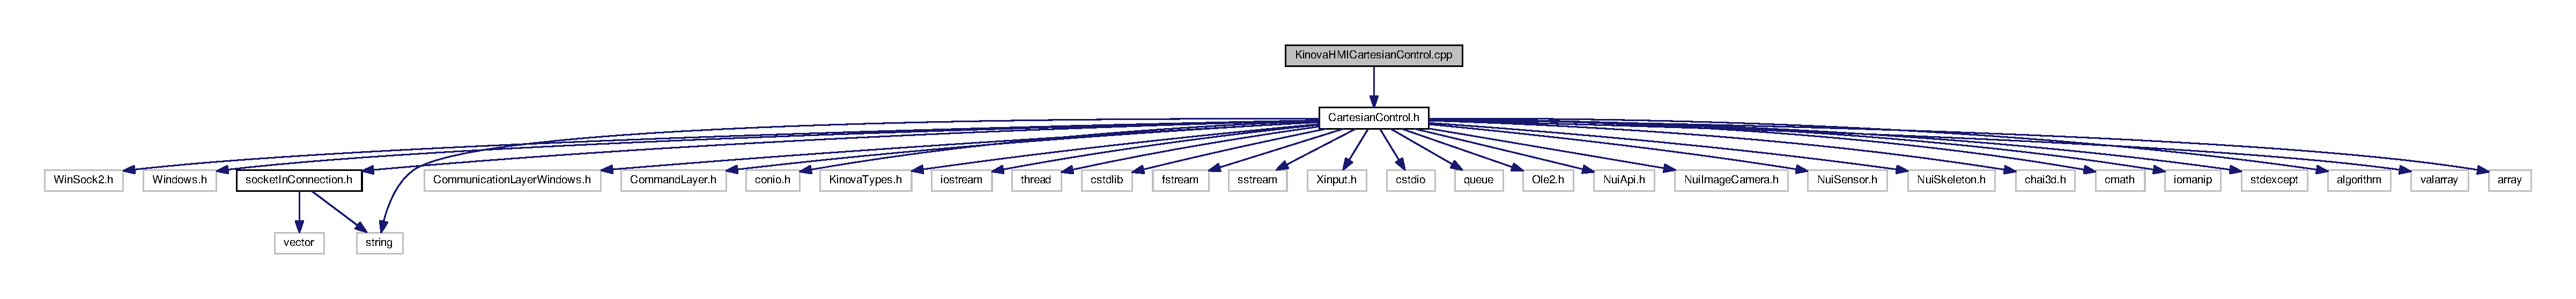
\includegraphics[width=350pt]{d3/da6/KinovaHMICartesianControl_2KinovaHMICartesianControl_8cpp__incl}
\end{center}
\end{figure}
\subsection*{Functions}
\begin{DoxyCompactItemize}
\item 
int \hyperlink{KinovaHMICartesianControl_2KinovaHMICartesianControl_8cpp_a0ddf1224851353fc92bfbff6f499fa97}{main} (int argc, char $\ast$argv\mbox{[}$\,$\mbox{]})
\end{DoxyCompactItemize}
\subsection*{Variables}
\begin{DoxyCompactItemize}
\item 
 H\+I\+N\+S\+T\+A\+N\+CE \hyperlink{KinovaHMICartesianControl_2KinovaHMICartesianControl_8cpp_a7dcbafc298af1cba5defa0baf9cfb948}{command\+Layer\+\_\+handle}
\end{DoxyCompactItemize}


\subsection{Function Documentation}
\index{Kinova\+H\+M\+I\+Cartesian\+Control/\+Kinova\+H\+M\+I\+Cartesian\+Control.\+cpp@{Kinova\+H\+M\+I\+Cartesian\+Control/\+Kinova\+H\+M\+I\+Cartesian\+Control.\+cpp}!main@{main}}
\index{main@{main}!Kinova\+H\+M\+I\+Cartesian\+Control/\+Kinova\+H\+M\+I\+Cartesian\+Control.\+cpp@{Kinova\+H\+M\+I\+Cartesian\+Control/\+Kinova\+H\+M\+I\+Cartesian\+Control.\+cpp}}
\subsubsection[{\texorpdfstring{main(int argc, char $\ast$argv[])}{main(int argc, char *argv[])}}]{\setlength{\rightskip}{0pt plus 5cm}int main (
\begin{DoxyParamCaption}
\item[{int}]{argc, }
\item[{char $\ast$}]{argv\mbox{[}$\,$\mbox{]}}
\end{DoxyParamCaption}
)}\hypertarget{KinovaHMICartesianControl_2KinovaHMICartesianControl_8cpp_a0ddf1224851353fc92bfbff6f499fa97}{}\label{KinovaHMICartesianControl_2KinovaHMICartesianControl_8cpp_a0ddf1224851353fc92bfbff6f499fa97}


\subsection{Variable Documentation}
\index{Kinova\+H\+M\+I\+Cartesian\+Control/\+Kinova\+H\+M\+I\+Cartesian\+Control.\+cpp@{Kinova\+H\+M\+I\+Cartesian\+Control/\+Kinova\+H\+M\+I\+Cartesian\+Control.\+cpp}!command\+Layer\+\_\+handle@{command\+Layer\+\_\+handle}}
\index{command\+Layer\+\_\+handle@{command\+Layer\+\_\+handle}!Kinova\+H\+M\+I\+Cartesian\+Control/\+Kinova\+H\+M\+I\+Cartesian\+Control.\+cpp@{Kinova\+H\+M\+I\+Cartesian\+Control/\+Kinova\+H\+M\+I\+Cartesian\+Control.\+cpp}}
\subsubsection[{\texorpdfstring{command\+Layer\+\_\+handle}{commandLayer_handle}}]{\setlength{\rightskip}{0pt plus 5cm} H\+I\+N\+S\+T\+A\+N\+CE command\+Layer\+\_\+handle}\hypertarget{KinovaHMICartesianControl_2KinovaHMICartesianControl_8cpp_a7dcbafc298af1cba5defa0baf9cfb948}{}\label{KinovaHMICartesianControl_2KinovaHMICartesianControl_8cpp_a7dcbafc298af1cba5defa0baf9cfb948}

\hypertarget{KinovaHMICartesianControl_8cpp}{}\section{Kinova\+H\+M\+I\+Cartesian\+Control.\+cpp File Reference}
\label{KinovaHMICartesianControl_8cpp}\index{Kinova\+H\+M\+I\+Cartesian\+Control.\+cpp@{Kinova\+H\+M\+I\+Cartesian\+Control.\+cpp}}
{\ttfamily \#include \char`\"{}Cartesian\+Control.\+h\char`\"{}}\\*
Include dependency graph for Kinova\+H\+M\+I\+Cartesian\+Control.\+cpp\+:\nopagebreak
\begin{figure}[H]
\begin{center}
\leavevmode
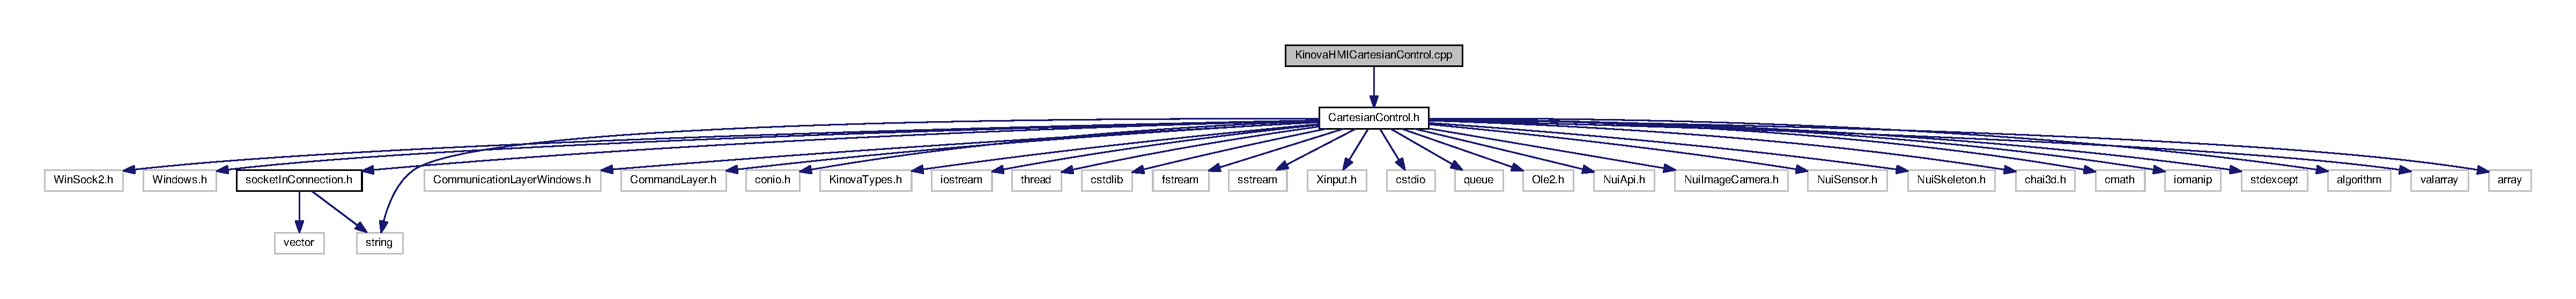
\includegraphics[width=350pt]{da/d8f/KinovaHMICartesianControl_8cpp__incl}
\end{center}
\end{figure}
\subsection*{Functions}
\begin{DoxyCompactItemize}
\item 
int \hyperlink{KinovaHMICartesianControl_8cpp_a0ddf1224851353fc92bfbff6f499fa97}{main} (int argc, char $\ast$argv\mbox{[}$\,$\mbox{]})
\end{DoxyCompactItemize}
\subsection*{Variables}
\begin{DoxyCompactItemize}
\item 
 H\+I\+N\+S\+T\+A\+N\+CE \hyperlink{KinovaHMICartesianControl_8cpp_a7dcbafc298af1cba5defa0baf9cfb948}{command\+Layer\+\_\+handle}
\end{DoxyCompactItemize}


\subsection{Function Documentation}
\index{Kinova\+H\+M\+I\+Cartesian\+Control.\+cpp@{Kinova\+H\+M\+I\+Cartesian\+Control.\+cpp}!main@{main}}
\index{main@{main}!Kinova\+H\+M\+I\+Cartesian\+Control.\+cpp@{Kinova\+H\+M\+I\+Cartesian\+Control.\+cpp}}
\subsubsection[{\texorpdfstring{main(int argc, char $\ast$argv[])}{main(int argc, char *argv[])}}]{\setlength{\rightskip}{0pt plus 5cm}int main (
\begin{DoxyParamCaption}
\item[{int}]{argc, }
\item[{char $\ast$}]{argv\mbox{[}$\,$\mbox{]}}
\end{DoxyParamCaption}
)}\hypertarget{KinovaHMICartesianControl_8cpp_a0ddf1224851353fc92bfbff6f499fa97}{}\label{KinovaHMICartesianControl_8cpp_a0ddf1224851353fc92bfbff6f499fa97}


\subsection{Variable Documentation}
\index{Kinova\+H\+M\+I\+Cartesian\+Control.\+cpp@{Kinova\+H\+M\+I\+Cartesian\+Control.\+cpp}!command\+Layer\+\_\+handle@{command\+Layer\+\_\+handle}}
\index{command\+Layer\+\_\+handle@{command\+Layer\+\_\+handle}!Kinova\+H\+M\+I\+Cartesian\+Control.\+cpp@{Kinova\+H\+M\+I\+Cartesian\+Control.\+cpp}}
\subsubsection[{\texorpdfstring{command\+Layer\+\_\+handle}{commandLayer_handle}}]{\setlength{\rightskip}{0pt plus 5cm} H\+I\+N\+S\+T\+A\+N\+CE command\+Layer\+\_\+handle}\hypertarget{KinovaHMICartesianControl_8cpp_a7dcbafc298af1cba5defa0baf9cfb948}{}\label{KinovaHMICartesianControl_8cpp_a7dcbafc298af1cba5defa0baf9cfb948}

\hypertarget{KinovaHMICartesianControl_2lutLinearInterp_8cpp}{}\section{lut\+Linear\+Interp.\+cpp File Reference}
\label{KinovaHMICartesianControl_2lutLinearInterp_8cpp}\index{lut\+Linear\+Interp.\+cpp@{lut\+Linear\+Interp.\+cpp}}
{\ttfamily \#include \char`\"{}stdafx.\+h\char`\"{}}\\*
{\ttfamily \#include \char`\"{}Cartesian\+Control.\+h\char`\"{}}\\*
Include dependency graph for Kinova\+H\+M\+I\+Cartesian\+Control/lut\+Linear\+Interp.cpp\+:
\nopagebreak
\begin{figure}[H]
\begin{center}
\leavevmode
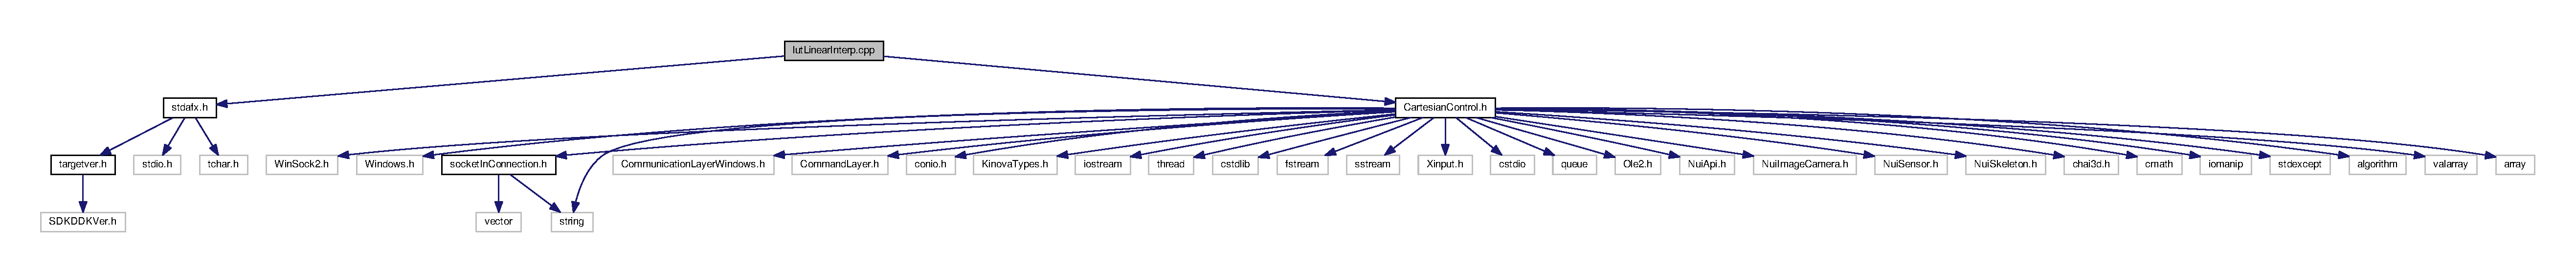
\includegraphics[width=350pt]{db/dfa/KinovaHMICartesianControl_2lutLinearInterp_8cpp__incl}
\end{center}
\end{figure}
\subsection*{Macros}
\begin{DoxyCompactItemize}
\item 
\#define \hyperlink{KinovaHMICartesianControl_2lutLinearInterp_8cpp_adfc8f90f3a8caa8423099cf36ff214f1}{\+\_\+\+W\+I\+N\+S\+O\+C\+K\+\_\+\+D\+E\+P\+R\+E\+C\+A\+T\+E\+D\+\_\+\+N\+O\+\_\+\+W\+A\+R\+N\+I\+N\+GS}
\item 
\#define \hyperlink{KinovaHMICartesianControl_2lutLinearInterp_8cpp_ac7bef5d85e3dcd73eef56ad39ffc84a9}{W\+I\+N32\+\_\+\+L\+E\+A\+N\+\_\+\+A\+N\+D\+\_\+\+M\+E\+AN}
\end{DoxyCompactItemize}


\subsection{Macro Definition Documentation}
\index{Kinova\+H\+M\+I\+Cartesian\+Control/lut\+Linear\+Interp.\+cpp@{Kinova\+H\+M\+I\+Cartesian\+Control/lut\+Linear\+Interp.\+cpp}!\+\_\+\+W\+I\+N\+S\+O\+C\+K\+\_\+\+D\+E\+P\+R\+E\+C\+A\+T\+E\+D\+\_\+\+N\+O\+\_\+\+W\+A\+R\+N\+I\+N\+GS@{\+\_\+\+W\+I\+N\+S\+O\+C\+K\+\_\+\+D\+E\+P\+R\+E\+C\+A\+T\+E\+D\+\_\+\+N\+O\+\_\+\+W\+A\+R\+N\+I\+N\+GS}}
\index{\+\_\+\+W\+I\+N\+S\+O\+C\+K\+\_\+\+D\+E\+P\+R\+E\+C\+A\+T\+E\+D\+\_\+\+N\+O\+\_\+\+W\+A\+R\+N\+I\+N\+GS@{\+\_\+\+W\+I\+N\+S\+O\+C\+K\+\_\+\+D\+E\+P\+R\+E\+C\+A\+T\+E\+D\+\_\+\+N\+O\+\_\+\+W\+A\+R\+N\+I\+N\+GS}!Kinova\+H\+M\+I\+Cartesian\+Control/lut\+Linear\+Interp.\+cpp@{Kinova\+H\+M\+I\+Cartesian\+Control/lut\+Linear\+Interp.\+cpp}}
\subsubsection[{\texorpdfstring{\+\_\+\+W\+I\+N\+S\+O\+C\+K\+\_\+\+D\+E\+P\+R\+E\+C\+A\+T\+E\+D\+\_\+\+N\+O\+\_\+\+W\+A\+R\+N\+I\+N\+GS}{_WINSOCK_DEPRECATED_NO_WARNINGS}}]{\setlength{\rightskip}{0pt plus 5cm}\#define \+\_\+\+W\+I\+N\+S\+O\+C\+K\+\_\+\+D\+E\+P\+R\+E\+C\+A\+T\+E\+D\+\_\+\+N\+O\+\_\+\+W\+A\+R\+N\+I\+N\+GS}\hypertarget{KinovaHMICartesianControl_2lutLinearInterp_8cpp_adfc8f90f3a8caa8423099cf36ff214f1}{}\label{KinovaHMICartesianControl_2lutLinearInterp_8cpp_adfc8f90f3a8caa8423099cf36ff214f1}
\index{Kinova\+H\+M\+I\+Cartesian\+Control/lut\+Linear\+Interp.\+cpp@{Kinova\+H\+M\+I\+Cartesian\+Control/lut\+Linear\+Interp.\+cpp}!W\+I\+N32\+\_\+\+L\+E\+A\+N\+\_\+\+A\+N\+D\+\_\+\+M\+E\+AN@{W\+I\+N32\+\_\+\+L\+E\+A\+N\+\_\+\+A\+N\+D\+\_\+\+M\+E\+AN}}
\index{W\+I\+N32\+\_\+\+L\+E\+A\+N\+\_\+\+A\+N\+D\+\_\+\+M\+E\+AN@{W\+I\+N32\+\_\+\+L\+E\+A\+N\+\_\+\+A\+N\+D\+\_\+\+M\+E\+AN}!Kinova\+H\+M\+I\+Cartesian\+Control/lut\+Linear\+Interp.\+cpp@{Kinova\+H\+M\+I\+Cartesian\+Control/lut\+Linear\+Interp.\+cpp}}
\subsubsection[{\texorpdfstring{W\+I\+N32\+\_\+\+L\+E\+A\+N\+\_\+\+A\+N\+D\+\_\+\+M\+E\+AN}{WIN32_LEAN_AND_MEAN}}]{\setlength{\rightskip}{0pt plus 5cm}\#define W\+I\+N32\+\_\+\+L\+E\+A\+N\+\_\+\+A\+N\+D\+\_\+\+M\+E\+AN}\hypertarget{KinovaHMICartesianControl_2lutLinearInterp_8cpp_ac7bef5d85e3dcd73eef56ad39ffc84a9}{}\label{KinovaHMICartesianControl_2lutLinearInterp_8cpp_ac7bef5d85e3dcd73eef56ad39ffc84a9}

\hypertarget{lutLinearInterp_8cpp}{}\section{lut\+Linear\+Interp.\+cpp File Reference}
\label{lutLinearInterp_8cpp}\index{lut\+Linear\+Interp.\+cpp@{lut\+Linear\+Interp.\+cpp}}
{\ttfamily \#include \char`\"{}stdafx.\+h\char`\"{}}\\*
{\ttfamily \#include \char`\"{}Cartesian\+Control.\+h\char`\"{}}\\*
Include dependency graph for lut\+Linear\+Interp.\+cpp\+:\nopagebreak
\begin{figure}[H]
\begin{center}
\leavevmode
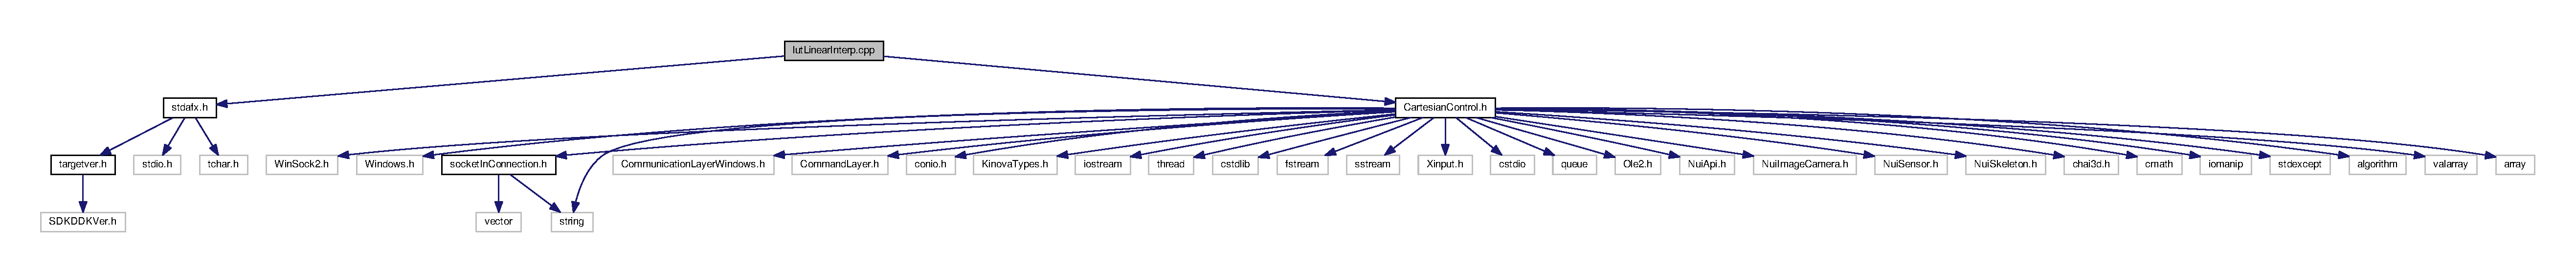
\includegraphics[width=350pt]{dc/d54/lutLinearInterp_8cpp__incl}
\end{center}
\end{figure}
\subsection*{Macros}
\begin{DoxyCompactItemize}
\item 
\#define \hyperlink{lutLinearInterp_8cpp_adfc8f90f3a8caa8423099cf36ff214f1}{\+\_\+\+W\+I\+N\+S\+O\+C\+K\+\_\+\+D\+E\+P\+R\+E\+C\+A\+T\+E\+D\+\_\+\+N\+O\+\_\+\+W\+A\+R\+N\+I\+N\+GS}
\item 
\#define \hyperlink{lutLinearInterp_8cpp_ac7bef5d85e3dcd73eef56ad39ffc84a9}{W\+I\+N32\+\_\+\+L\+E\+A\+N\+\_\+\+A\+N\+D\+\_\+\+M\+E\+AN}
\end{DoxyCompactItemize}


\subsection{Macro Definition Documentation}
\index{lut\+Linear\+Interp.\+cpp@{lut\+Linear\+Interp.\+cpp}!\+\_\+\+W\+I\+N\+S\+O\+C\+K\+\_\+\+D\+E\+P\+R\+E\+C\+A\+T\+E\+D\+\_\+\+N\+O\+\_\+\+W\+A\+R\+N\+I\+N\+GS@{\+\_\+\+W\+I\+N\+S\+O\+C\+K\+\_\+\+D\+E\+P\+R\+E\+C\+A\+T\+E\+D\+\_\+\+N\+O\+\_\+\+W\+A\+R\+N\+I\+N\+GS}}
\index{\+\_\+\+W\+I\+N\+S\+O\+C\+K\+\_\+\+D\+E\+P\+R\+E\+C\+A\+T\+E\+D\+\_\+\+N\+O\+\_\+\+W\+A\+R\+N\+I\+N\+GS@{\+\_\+\+W\+I\+N\+S\+O\+C\+K\+\_\+\+D\+E\+P\+R\+E\+C\+A\+T\+E\+D\+\_\+\+N\+O\+\_\+\+W\+A\+R\+N\+I\+N\+GS}!lut\+Linear\+Interp.\+cpp@{lut\+Linear\+Interp.\+cpp}}
\subsubsection[{\texorpdfstring{\+\_\+\+W\+I\+N\+S\+O\+C\+K\+\_\+\+D\+E\+P\+R\+E\+C\+A\+T\+E\+D\+\_\+\+N\+O\+\_\+\+W\+A\+R\+N\+I\+N\+GS}{_WINSOCK_DEPRECATED_NO_WARNINGS}}]{\setlength{\rightskip}{0pt plus 5cm}\#define \+\_\+\+W\+I\+N\+S\+O\+C\+K\+\_\+\+D\+E\+P\+R\+E\+C\+A\+T\+E\+D\+\_\+\+N\+O\+\_\+\+W\+A\+R\+N\+I\+N\+GS}\hypertarget{lutLinearInterp_8cpp_adfc8f90f3a8caa8423099cf36ff214f1}{}\label{lutLinearInterp_8cpp_adfc8f90f3a8caa8423099cf36ff214f1}
\index{lut\+Linear\+Interp.\+cpp@{lut\+Linear\+Interp.\+cpp}!W\+I\+N32\+\_\+\+L\+E\+A\+N\+\_\+\+A\+N\+D\+\_\+\+M\+E\+AN@{W\+I\+N32\+\_\+\+L\+E\+A\+N\+\_\+\+A\+N\+D\+\_\+\+M\+E\+AN}}
\index{W\+I\+N32\+\_\+\+L\+E\+A\+N\+\_\+\+A\+N\+D\+\_\+\+M\+E\+AN@{W\+I\+N32\+\_\+\+L\+E\+A\+N\+\_\+\+A\+N\+D\+\_\+\+M\+E\+AN}!lut\+Linear\+Interp.\+cpp@{lut\+Linear\+Interp.\+cpp}}
\subsubsection[{\texorpdfstring{W\+I\+N32\+\_\+\+L\+E\+A\+N\+\_\+\+A\+N\+D\+\_\+\+M\+E\+AN}{WIN32_LEAN_AND_MEAN}}]{\setlength{\rightskip}{0pt plus 5cm}\#define W\+I\+N32\+\_\+\+L\+E\+A\+N\+\_\+\+A\+N\+D\+\_\+\+M\+E\+AN}\hypertarget{lutLinearInterp_8cpp_ac7bef5d85e3dcd73eef56ad39ffc84a9}{}\label{lutLinearInterp_8cpp_ac7bef5d85e3dcd73eef56ad39ffc84a9}

\hypertarget{pages__0_8js}{}\section{pages\+\_\+0.\+js File Reference}
\label{pages__0_8js}\index{pages\+\_\+0.\+js@{pages\+\_\+0.\+js}}
\subsection*{Variables}
\begin{DoxyCompactItemize}
\item 
var \hyperlink{pages__0_8js_ad01a7523f103d6242ef9b0451861231e}{search\+Data}
\end{DoxyCompactItemize}


\subsection{Variable Documentation}
\index{pages\+\_\+0.\+js@{pages\+\_\+0.\+js}!search\+Data@{search\+Data}}
\index{search\+Data@{search\+Data}!pages\+\_\+0.\+js@{pages\+\_\+0.\+js}}
\subsubsection[{\texorpdfstring{search\+Data}{searchData}}]{\setlength{\rightskip}{0pt plus 5cm}var search\+Data}\hypertarget{pages__0_8js_ad01a7523f103d6242ef9b0451861231e}{}\label{pages__0_8js_ad01a7523f103d6242ef9b0451861231e}
{\bfseries Initial value\+:}
\begin{DoxyCode}
=
[
  [\textcolor{stringliteral}{'getting\_20started'},[\textcolor{stringliteral}{'Getting Started'},[\textcolor{stringliteral}{'../gettingstarted.html'},1,\textcolor{stringliteral}{''}]]]
]
\end{DoxyCode}

\hypertarget{pages__1_8js}{}\section{pages\+\_\+1.\+js File Reference}
\label{pages__1_8js}\index{pages\+\_\+1.\+js@{pages\+\_\+1.\+js}}
\subsection*{Variables}
\begin{DoxyCompactItemize}
\item 
var \hyperlink{pages__1_8js_ad01a7523f103d6242ef9b0451861231e}{search\+Data}
\end{DoxyCompactItemize}


\subsection{Variable Documentation}
\index{pages\+\_\+1.\+js@{pages\+\_\+1.\+js}!search\+Data@{search\+Data}}
\index{search\+Data@{search\+Data}!pages\+\_\+1.\+js@{pages\+\_\+1.\+js}}
\subsubsection[{\texorpdfstring{search\+Data}{searchData}}]{\setlength{\rightskip}{0pt plus 5cm}var search\+Data}\hypertarget{pages__1_8js_ad01a7523f103d6242ef9b0451861231e}{}\label{pages__1_8js_ad01a7523f103d6242ef9b0451861231e}
{\bfseries Initial value\+:}
\begin{DoxyCode}
=
[
  [\textcolor{stringliteral}{'introduction'},[\textcolor{stringliteral}{'Introduction'},[\textcolor{stringliteral}{'../index.html'},1,\textcolor{stringliteral}{''}]]],
  [\textcolor{stringliteral}{'installation\_20notes'},[\textcolor{stringliteral}{'Installation Notes'},[\textcolor{stringliteral}{'../install.html'},1,\textcolor{stringliteral}{'index'}]]]
]
\end{DoxyCode}

\hypertarget{pages__2_8js}{}\section{pages\+\_\+2.\+js File Reference}
\label{pages__2_8js}\index{pages\+\_\+2.\+js@{pages\+\_\+2.\+js}}
\subsection*{Variables}
\begin{DoxyCompactItemize}
\item 
var \hyperlink{pages__2_8js_ad01a7523f103d6242ef9b0451861231e}{search\+Data}
\end{DoxyCompactItemize}


\subsection{Variable Documentation}
\index{pages\+\_\+2.\+js@{pages\+\_\+2.\+js}!search\+Data@{search\+Data}}
\index{search\+Data@{search\+Data}!pages\+\_\+2.\+js@{pages\+\_\+2.\+js}}
\subsubsection[{\texorpdfstring{search\+Data}{searchData}}]{\setlength{\rightskip}{0pt plus 5cm}var search\+Data}\hypertarget{pages__2_8js_ad01a7523f103d6242ef9b0451861231e}{}\label{pages__2_8js_ad01a7523f103d6242ef9b0451861231e}
{\bfseries Initial value\+:}
\begin{DoxyCode}
=
[
  [\textcolor{stringliteral}{'overview'},[\textcolor{stringliteral}{'Overview'},[\textcolor{stringliteral}{'../overview.html'},1,\textcolor{stringliteral}{''}]]]
]
\end{DoxyCode}

\hypertarget{pages__3_8js}{}\section{pages\+\_\+3.\+js File Reference}
\label{pages__3_8js}\index{pages\+\_\+3.\+js@{pages\+\_\+3.\+js}}
\subsection*{Variables}
\begin{DoxyCompactItemize}
\item 
var \hyperlink{pages__3_8js_ad01a7523f103d6242ef9b0451861231e}{search\+Data}
\end{DoxyCompactItemize}


\subsection{Variable Documentation}
\index{pages\+\_\+3.\+js@{pages\+\_\+3.\+js}!search\+Data@{search\+Data}}
\index{search\+Data@{search\+Data}!pages\+\_\+3.\+js@{pages\+\_\+3.\+js}}
\subsubsection[{\texorpdfstring{search\+Data}{searchData}}]{\setlength{\rightskip}{0pt plus 5cm}var search\+Data}\hypertarget{pages__3_8js_ad01a7523f103d6242ef9b0451861231e}{}\label{pages__3_8js_ad01a7523f103d6242ef9b0451861231e}
{\bfseries Initial value\+:}
\begin{DoxyCode}
=
[
  [\textcolor{stringliteral}{'references'},[\textcolor{stringliteral}{'References'},[\textcolor{stringliteral}{'../references.html'},1,\textcolor{stringliteral}{''}]]]
]
\end{DoxyCode}

\hypertarget{pages__4_8js}{}\section{pages\+\_\+4.\+js File Reference}
\label{pages__4_8js}\index{pages\+\_\+4.\+js@{pages\+\_\+4.\+js}}
\subsection*{Variables}
\begin{DoxyCompactItemize}
\item 
var \hyperlink{pages__4_8js_ad01a7523f103d6242ef9b0451861231e}{search\+Data}
\end{DoxyCompactItemize}


\subsection{Variable Documentation}
\index{pages\+\_\+4.\+js@{pages\+\_\+4.\+js}!search\+Data@{search\+Data}}
\index{search\+Data@{search\+Data}!pages\+\_\+4.\+js@{pages\+\_\+4.\+js}}
\subsubsection[{\texorpdfstring{search\+Data}{searchData}}]{\setlength{\rightskip}{0pt plus 5cm}var search\+Data}\hypertarget{pages__4_8js_ad01a7523f103d6242ef9b0451861231e}{}\label{pages__4_8js_ad01a7523f103d6242ef9b0451861231e}
{\bfseries Initial value\+:}
\begin{DoxyCode}
=
[
  [\textcolor{stringliteral}{'software\_20license'},[\textcolor{stringliteral}{'Software License'},[\textcolor{stringliteral}{'../license.html'},1,\textcolor{stringliteral}{'index'}]]]
]
\end{DoxyCode}

\hypertarget{pages__5_8js}{}\section{pages\+\_\+5.\+js File Reference}
\label{pages__5_8js}\index{pages\+\_\+5.\+js@{pages\+\_\+5.\+js}}
\subsection*{Variables}
\begin{DoxyCompactItemize}
\item 
var \hyperlink{pages__5_8js_ad01a7523f103d6242ef9b0451861231e}{search\+Data}
\end{DoxyCompactItemize}


\subsection{Variable Documentation}
\index{pages\+\_\+5.\+js@{pages\+\_\+5.\+js}!search\+Data@{search\+Data}}
\index{search\+Data@{search\+Data}!pages\+\_\+5.\+js@{pages\+\_\+5.\+js}}
\subsubsection[{\texorpdfstring{search\+Data}{searchData}}]{\setlength{\rightskip}{0pt plus 5cm}var search\+Data}\hypertarget{pages__5_8js_ad01a7523f103d6242ef9b0451861231e}{}\label{pages__5_8js_ad01a7523f103d6242ef9b0451861231e}
{\bfseries Initial value\+:}
\begin{DoxyCode}
=
[
  [\textcolor{stringliteral}{'software\_20license'},[\textcolor{stringliteral}{'Software License'},[\textcolor{stringliteral}{'../license.html'},1,\textcolor{stringliteral}{'index'}]]]
]
\end{DoxyCode}

\hypertarget{search_8js}{}\section{search.\+js File Reference}
\label{search_8js}\index{search.\+js@{search.\+js}}
\subsection*{Functions}
\begin{DoxyCompactItemize}
\item 
function \hyperlink{search_8js_a196a29bd5a5ee7cd5b485e0753a49e57}{convert\+To\+Id} (search)
\item 
function \hyperlink{search_8js_a76d24aea0009f892f8ccc31d941c0a2b}{get\+X\+Pos} (item)
\item 
function \hyperlink{search_8js_a8d7b405228661d7b6216b6925d2b8a69}{get\+Y\+Pos} (item)
\item 
function \hyperlink{search_8js_a52066106482f8136aa9e0ec859e8188f}{Search\+Box} (name, results\+Path, in\+Frame, label)
\item 
function \hyperlink{search_8js_a9189b9f7a32b6bc78240f40348f7fe03}{Search\+Results} (name)
\item 
function \hyperlink{search_8js_a98192fa2929bb8e4b0a890a4909ab9b2}{set\+Key\+Actions} (elem, action)
\item 
function \hyperlink{search_8js_a499422fc054a5278ae32801ec0082c56}{set\+Class\+Attr} (elem, attr)
\item 
function \hyperlink{search_8js_a6b2c651120de3ed1dcf0d85341d51895}{create\+Results} ()
\item 
function \hyperlink{search_8js_ae95ec7d5d450d0a8d6928a594798aaf4}{init\+\_\+search} ()
\end{DoxyCompactItemize}


\subsection{Function Documentation}
\index{search.\+js@{search.\+js}!convert\+To\+Id@{convert\+To\+Id}}
\index{convert\+To\+Id@{convert\+To\+Id}!search.\+js@{search.\+js}}
\subsubsection[{\texorpdfstring{convert\+To\+Id(search)}{convertToId(search)}}]{\setlength{\rightskip}{0pt plus 5cm}function convert\+To\+Id (
\begin{DoxyParamCaption}
\item[{}]{search}
\end{DoxyParamCaption}
)}\hypertarget{search_8js_a196a29bd5a5ee7cd5b485e0753a49e57}{}\label{search_8js_a196a29bd5a5ee7cd5b485e0753a49e57}
\index{search.\+js@{search.\+js}!create\+Results@{create\+Results}}
\index{create\+Results@{create\+Results}!search.\+js@{search.\+js}}
\subsubsection[{\texorpdfstring{create\+Results()}{createResults()}}]{\setlength{\rightskip}{0pt plus 5cm}function create\+Results (
\begin{DoxyParamCaption}
{}
\end{DoxyParamCaption}
)}\hypertarget{search_8js_a6b2c651120de3ed1dcf0d85341d51895}{}\label{search_8js_a6b2c651120de3ed1dcf0d85341d51895}
\index{search.\+js@{search.\+js}!get\+X\+Pos@{get\+X\+Pos}}
\index{get\+X\+Pos@{get\+X\+Pos}!search.\+js@{search.\+js}}
\subsubsection[{\texorpdfstring{get\+X\+Pos(item)}{getXPos(item)}}]{\setlength{\rightskip}{0pt plus 5cm}function get\+X\+Pos (
\begin{DoxyParamCaption}
\item[{}]{item}
\end{DoxyParamCaption}
)}\hypertarget{search_8js_a76d24aea0009f892f8ccc31d941c0a2b}{}\label{search_8js_a76d24aea0009f892f8ccc31d941c0a2b}
\index{search.\+js@{search.\+js}!get\+Y\+Pos@{get\+Y\+Pos}}
\index{get\+Y\+Pos@{get\+Y\+Pos}!search.\+js@{search.\+js}}
\subsubsection[{\texorpdfstring{get\+Y\+Pos(item)}{getYPos(item)}}]{\setlength{\rightskip}{0pt plus 5cm}function get\+Y\+Pos (
\begin{DoxyParamCaption}
\item[{}]{item}
\end{DoxyParamCaption}
)}\hypertarget{search_8js_a8d7b405228661d7b6216b6925d2b8a69}{}\label{search_8js_a8d7b405228661d7b6216b6925d2b8a69}
\index{search.\+js@{search.\+js}!init\+\_\+search@{init\+\_\+search}}
\index{init\+\_\+search@{init\+\_\+search}!search.\+js@{search.\+js}}
\subsubsection[{\texorpdfstring{init\+\_\+search()}{init_search()}}]{\setlength{\rightskip}{0pt plus 5cm}function init\+\_\+search (
\begin{DoxyParamCaption}
{}
\end{DoxyParamCaption}
)}\hypertarget{search_8js_ae95ec7d5d450d0a8d6928a594798aaf4}{}\label{search_8js_ae95ec7d5d450d0a8d6928a594798aaf4}
\index{search.\+js@{search.\+js}!Search\+Box@{Search\+Box}}
\index{Search\+Box@{Search\+Box}!search.\+js@{search.\+js}}
\subsubsection[{\texorpdfstring{Search\+Box(name, results\+Path, in\+Frame, label)}{SearchBox(name, resultsPath, inFrame, label)}}]{\setlength{\rightskip}{0pt plus 5cm}function Search\+Box (
\begin{DoxyParamCaption}
\item[{}]{name, }
\item[{}]{results\+Path, }
\item[{}]{in\+Frame, }
\item[{}]{label}
\end{DoxyParamCaption}
)}\hypertarget{search_8js_a52066106482f8136aa9e0ec859e8188f}{}\label{search_8js_a52066106482f8136aa9e0ec859e8188f}
\index{search.\+js@{search.\+js}!Search\+Results@{Search\+Results}}
\index{Search\+Results@{Search\+Results}!search.\+js@{search.\+js}}
\subsubsection[{\texorpdfstring{Search\+Results(name)}{SearchResults(name)}}]{\setlength{\rightskip}{0pt plus 5cm}function Search\+Results (
\begin{DoxyParamCaption}
\item[{}]{name}
\end{DoxyParamCaption}
)}\hypertarget{search_8js_a9189b9f7a32b6bc78240f40348f7fe03}{}\label{search_8js_a9189b9f7a32b6bc78240f40348f7fe03}
\index{search.\+js@{search.\+js}!set\+Class\+Attr@{set\+Class\+Attr}}
\index{set\+Class\+Attr@{set\+Class\+Attr}!search.\+js@{search.\+js}}
\subsubsection[{\texorpdfstring{set\+Class\+Attr(elem, attr)}{setClassAttr(elem, attr)}}]{\setlength{\rightskip}{0pt plus 5cm}function set\+Class\+Attr (
\begin{DoxyParamCaption}
\item[{}]{elem, }
\item[{}]{attr}
\end{DoxyParamCaption}
)}\hypertarget{search_8js_a499422fc054a5278ae32801ec0082c56}{}\label{search_8js_a499422fc054a5278ae32801ec0082c56}
\index{search.\+js@{search.\+js}!set\+Key\+Actions@{set\+Key\+Actions}}
\index{set\+Key\+Actions@{set\+Key\+Actions}!search.\+js@{search.\+js}}
\subsubsection[{\texorpdfstring{set\+Key\+Actions(elem, action)}{setKeyActions(elem, action)}}]{\setlength{\rightskip}{0pt plus 5cm}function set\+Key\+Actions (
\begin{DoxyParamCaption}
\item[{}]{elem, }
\item[{}]{action}
\end{DoxyParamCaption}
)}\hypertarget{search_8js_a98192fa2929bb8e4b0a890a4909ab9b2}{}\label{search_8js_a98192fa2929bb8e4b0a890a4909ab9b2}

\hypertarget{searchdata_8js}{}\section{searchdata.\+js File Reference}
\label{searchdata_8js}\index{searchdata.\+js@{searchdata.\+js}}
\subsection*{Variables}
\begin{DoxyCompactItemize}
\item 
var \hyperlink{searchdata_8js_a6250af3c9b54dee6efc5f55f40c78126}{index\+Sections\+With\+Content}
\item 
var \hyperlink{searchdata_8js_a77149ceed055c6c6ce40973b5bdc19ad}{index\+Section\+Names}
\item 
var \hyperlink{searchdata_8js_a529972e449c82dc118cbbd3bcf50c44d}{index\+Section\+Labels}
\end{DoxyCompactItemize}


\subsection{Variable Documentation}
\index{searchdata.\+js@{searchdata.\+js}!index\+Section\+Labels@{index\+Section\+Labels}}
\index{index\+Section\+Labels@{index\+Section\+Labels}!searchdata.\+js@{searchdata.\+js}}
\subsubsection[{\texorpdfstring{index\+Section\+Labels}{indexSectionLabels}}]{\setlength{\rightskip}{0pt plus 5cm}var index\+Section\+Labels}\hypertarget{searchdata_8js_a529972e449c82dc118cbbd3bcf50c44d}{}\label{searchdata_8js_a529972e449c82dc118cbbd3bcf50c44d}
{\bfseries Initial value\+:}
\begin{DoxyCode}
=
\{
  0: \textcolor{stringliteral}{"All"},
  1: \textcolor{stringliteral}{"Classes"},
  2: \textcolor{stringliteral}{"Files"},
  3: \textcolor{stringliteral}{"Functions"},
  4: \textcolor{stringliteral}{"Variables"},
  5: \textcolor{stringliteral}{"Macros"},
  6: \textcolor{stringliteral}{"Pages"}
\}
\end{DoxyCode}
\index{searchdata.\+js@{searchdata.\+js}!index\+Section\+Names@{index\+Section\+Names}}
\index{index\+Section\+Names@{index\+Section\+Names}!searchdata.\+js@{searchdata.\+js}}
\subsubsection[{\texorpdfstring{index\+Section\+Names}{indexSectionNames}}]{\setlength{\rightskip}{0pt plus 5cm}var index\+Section\+Names}\hypertarget{searchdata_8js_a77149ceed055c6c6ce40973b5bdc19ad}{}\label{searchdata_8js_a77149ceed055c6c6ce40973b5bdc19ad}
{\bfseries Initial value\+:}
\begin{DoxyCode}
=
\{
  0: \textcolor{stringliteral}{"all"},
  1: \textcolor{stringliteral}{"classes"},
  2: \textcolor{stringliteral}{"files"},
  3: \textcolor{stringliteral}{"functions"},
  4: \textcolor{stringliteral}{"variables"},
  5: \textcolor{stringliteral}{"defines"},
  6: \textcolor{stringliteral}{"pages"}
\}
\end{DoxyCode}
\index{searchdata.\+js@{searchdata.\+js}!index\+Sections\+With\+Content@{index\+Sections\+With\+Content}}
\index{index\+Sections\+With\+Content@{index\+Sections\+With\+Content}!searchdata.\+js@{searchdata.\+js}}
\subsubsection[{\texorpdfstring{index\+Sections\+With\+Content}{indexSectionsWithContent}}]{\setlength{\rightskip}{0pt plus 5cm}var index\+Sections\+With\+Content}\hypertarget{searchdata_8js_a6250af3c9b54dee6efc5f55f40c78126}{}\label{searchdata_8js_a6250af3c9b54dee6efc5f55f40c78126}
{\bfseries Initial value\+:}
\begin{DoxyCode}
=
\{
  0: \textcolor{stringliteral}{"\_abcdefghiklmnoprstuvw~"},
  1: \textcolor{stringliteral}{"cefknt"},
  2: \textcolor{stringliteral}{"acefhklst"},
  3: \textcolor{stringliteral}{"\_cefghilmrsuv~"},
  4: \textcolor{stringliteral}{"\_abcdfhiklmnoprstuw"},
  5: \textcolor{stringliteral}{"\_bghiltuw"},
  6: \textcolor{stringliteral}{"giors"}
\}
\end{DoxyCode}

\hypertarget{KinovaHMICartesianControl_2socketInConnection_8cpp}{}\section{socket\+In\+Connection.\+cpp File Reference}
\label{KinovaHMICartesianControl_2socketInConnection_8cpp}\index{socket\+In\+Connection.\+cpp@{socket\+In\+Connection.\+cpp}}
{\ttfamily \#include \char`\"{}stdafx.\+h\char`\"{}}\\*
{\ttfamily \#include \char`\"{}socket\+In\+Connection.\+h\char`\"{}}\\*
{\ttfamily \#include \char`\"{}Cartesian\+Control.\+h\char`\"{}}\\*
Include dependency graph for Kinova\+H\+M\+I\+Cartesian\+Control/socket\+In\+Connection.cpp\+:
\nopagebreak
\begin{figure}[H]
\begin{center}
\leavevmode
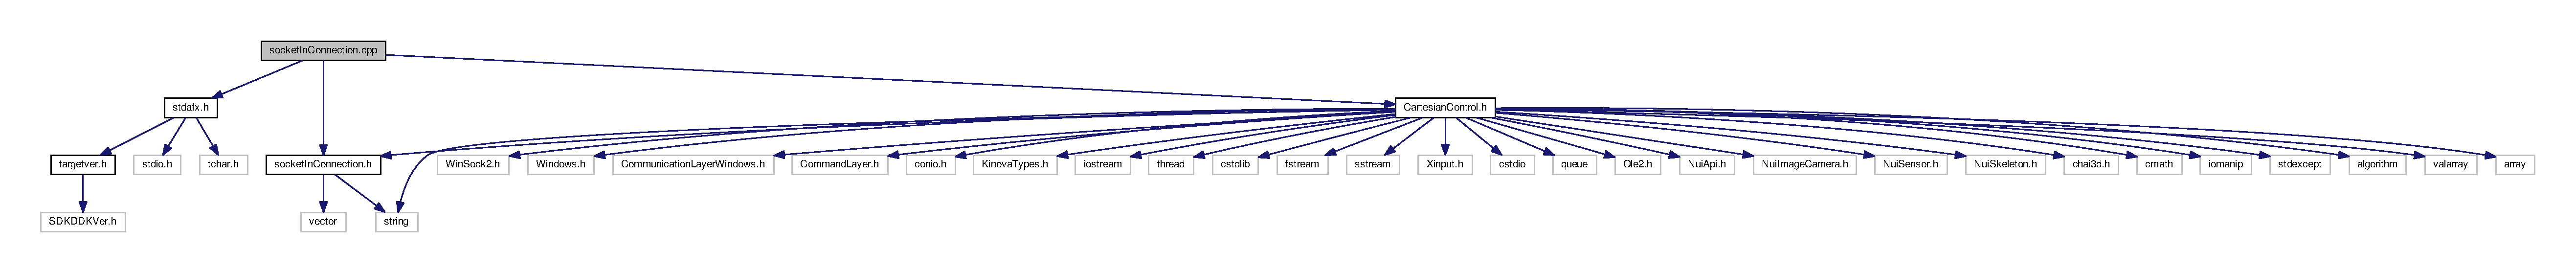
\includegraphics[width=350pt]{d8/d8c/KinovaHMICartesianControl_2socketInConnection_8cpp__incl}
\end{center}
\end{figure}
\subsection*{Macros}
\begin{DoxyCompactItemize}
\item 
\#define \hyperlink{KinovaHMICartesianControl_2socketInConnection_8cpp_adfc8f90f3a8caa8423099cf36ff214f1}{\+\_\+\+W\+I\+N\+S\+O\+C\+K\+\_\+\+D\+E\+P\+R\+E\+C\+A\+T\+E\+D\+\_\+\+N\+O\+\_\+\+W\+A\+R\+N\+I\+N\+GS}
\item 
\#define \hyperlink{KinovaHMICartesianControl_2socketInConnection_8cpp_acaf400df9a74b3295697ca29cc9261cb}{H\+E\+A\+D\+E\+R\+\_\+\+L\+E\+N\+G\+TH}~6
\end{DoxyCompactItemize}


\subsection{Macro Definition Documentation}
\index{Kinova\+H\+M\+I\+Cartesian\+Control/socket\+In\+Connection.\+cpp@{Kinova\+H\+M\+I\+Cartesian\+Control/socket\+In\+Connection.\+cpp}!\+\_\+\+W\+I\+N\+S\+O\+C\+K\+\_\+\+D\+E\+P\+R\+E\+C\+A\+T\+E\+D\+\_\+\+N\+O\+\_\+\+W\+A\+R\+N\+I\+N\+GS@{\+\_\+\+W\+I\+N\+S\+O\+C\+K\+\_\+\+D\+E\+P\+R\+E\+C\+A\+T\+E\+D\+\_\+\+N\+O\+\_\+\+W\+A\+R\+N\+I\+N\+GS}}
\index{\+\_\+\+W\+I\+N\+S\+O\+C\+K\+\_\+\+D\+E\+P\+R\+E\+C\+A\+T\+E\+D\+\_\+\+N\+O\+\_\+\+W\+A\+R\+N\+I\+N\+GS@{\+\_\+\+W\+I\+N\+S\+O\+C\+K\+\_\+\+D\+E\+P\+R\+E\+C\+A\+T\+E\+D\+\_\+\+N\+O\+\_\+\+W\+A\+R\+N\+I\+N\+GS}!Kinova\+H\+M\+I\+Cartesian\+Control/socket\+In\+Connection.\+cpp@{Kinova\+H\+M\+I\+Cartesian\+Control/socket\+In\+Connection.\+cpp}}
\subsubsection[{\texorpdfstring{\+\_\+\+W\+I\+N\+S\+O\+C\+K\+\_\+\+D\+E\+P\+R\+E\+C\+A\+T\+E\+D\+\_\+\+N\+O\+\_\+\+W\+A\+R\+N\+I\+N\+GS}{_WINSOCK_DEPRECATED_NO_WARNINGS}}]{\setlength{\rightskip}{0pt plus 5cm}\#define \+\_\+\+W\+I\+N\+S\+O\+C\+K\+\_\+\+D\+E\+P\+R\+E\+C\+A\+T\+E\+D\+\_\+\+N\+O\+\_\+\+W\+A\+R\+N\+I\+N\+GS}\hypertarget{KinovaHMICartesianControl_2socketInConnection_8cpp_adfc8f90f3a8caa8423099cf36ff214f1}{}\label{KinovaHMICartesianControl_2socketInConnection_8cpp_adfc8f90f3a8caa8423099cf36ff214f1}
\index{Kinova\+H\+M\+I\+Cartesian\+Control/socket\+In\+Connection.\+cpp@{Kinova\+H\+M\+I\+Cartesian\+Control/socket\+In\+Connection.\+cpp}!H\+E\+A\+D\+E\+R\+\_\+\+L\+E\+N\+G\+TH@{H\+E\+A\+D\+E\+R\+\_\+\+L\+E\+N\+G\+TH}}
\index{H\+E\+A\+D\+E\+R\+\_\+\+L\+E\+N\+G\+TH@{H\+E\+A\+D\+E\+R\+\_\+\+L\+E\+N\+G\+TH}!Kinova\+H\+M\+I\+Cartesian\+Control/socket\+In\+Connection.\+cpp@{Kinova\+H\+M\+I\+Cartesian\+Control/socket\+In\+Connection.\+cpp}}
\subsubsection[{\texorpdfstring{H\+E\+A\+D\+E\+R\+\_\+\+L\+E\+N\+G\+TH}{HEADER_LENGTH}}]{\setlength{\rightskip}{0pt plus 5cm}\#define H\+E\+A\+D\+E\+R\+\_\+\+L\+E\+N\+G\+TH~6}\hypertarget{KinovaHMICartesianControl_2socketInConnection_8cpp_acaf400df9a74b3295697ca29cc9261cb}{}\label{KinovaHMICartesianControl_2socketInConnection_8cpp_acaf400df9a74b3295697ca29cc9261cb}

\hypertarget{socketInConnection_8cpp}{}\section{socket\+In\+Connection.\+cpp File Reference}
\label{socketInConnection_8cpp}\index{socket\+In\+Connection.\+cpp@{socket\+In\+Connection.\+cpp}}
{\ttfamily \#include \char`\"{}stdafx.\+h\char`\"{}}\\*
{\ttfamily \#include \char`\"{}socket\+In\+Connection.\+h\char`\"{}}\\*
{\ttfamily \#include \char`\"{}Cartesian\+Control.\+h\char`\"{}}\\*
Include dependency graph for socket\+In\+Connection.\+cpp\+:\nopagebreak
\begin{figure}[H]
\begin{center}
\leavevmode
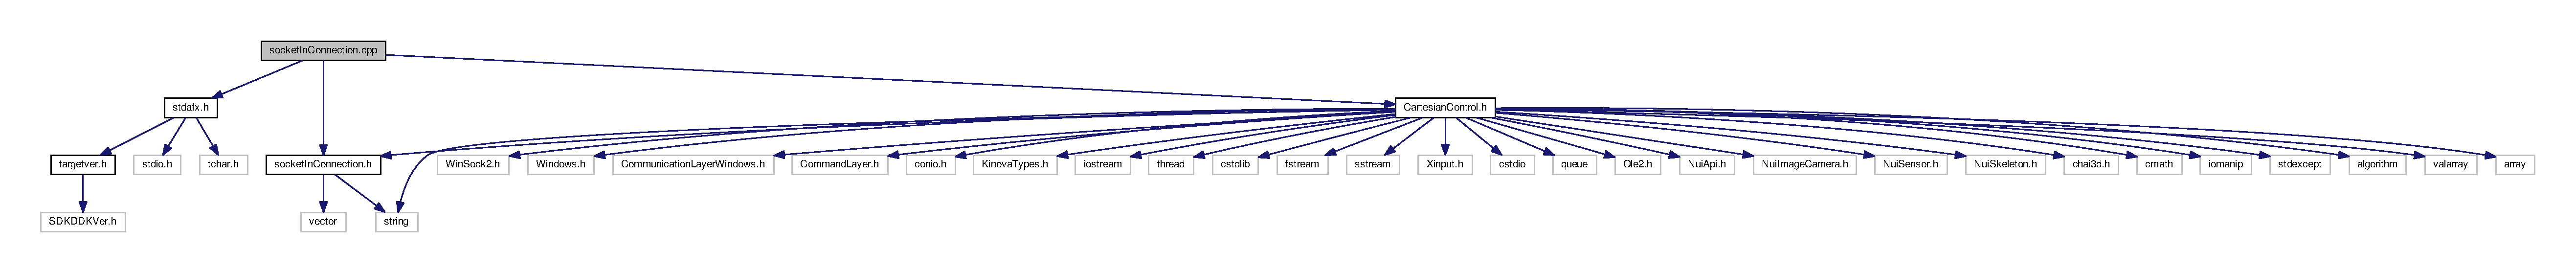
\includegraphics[width=350pt]{da/d9d/socketInConnection_8cpp__incl}
\end{center}
\end{figure}
\subsection*{Macros}
\begin{DoxyCompactItemize}
\item 
\#define \hyperlink{socketInConnection_8cpp_adfc8f90f3a8caa8423099cf36ff214f1}{\+\_\+\+W\+I\+N\+S\+O\+C\+K\+\_\+\+D\+E\+P\+R\+E\+C\+A\+T\+E\+D\+\_\+\+N\+O\+\_\+\+W\+A\+R\+N\+I\+N\+GS}
\item 
\#define \hyperlink{socketInConnection_8cpp_acaf400df9a74b3295697ca29cc9261cb}{H\+E\+A\+D\+E\+R\+\_\+\+L\+E\+N\+G\+TH}~6
\end{DoxyCompactItemize}


\subsection{Macro Definition Documentation}
\index{socket\+In\+Connection.\+cpp@{socket\+In\+Connection.\+cpp}!\+\_\+\+W\+I\+N\+S\+O\+C\+K\+\_\+\+D\+E\+P\+R\+E\+C\+A\+T\+E\+D\+\_\+\+N\+O\+\_\+\+W\+A\+R\+N\+I\+N\+GS@{\+\_\+\+W\+I\+N\+S\+O\+C\+K\+\_\+\+D\+E\+P\+R\+E\+C\+A\+T\+E\+D\+\_\+\+N\+O\+\_\+\+W\+A\+R\+N\+I\+N\+GS}}
\index{\+\_\+\+W\+I\+N\+S\+O\+C\+K\+\_\+\+D\+E\+P\+R\+E\+C\+A\+T\+E\+D\+\_\+\+N\+O\+\_\+\+W\+A\+R\+N\+I\+N\+GS@{\+\_\+\+W\+I\+N\+S\+O\+C\+K\+\_\+\+D\+E\+P\+R\+E\+C\+A\+T\+E\+D\+\_\+\+N\+O\+\_\+\+W\+A\+R\+N\+I\+N\+GS}!socket\+In\+Connection.\+cpp@{socket\+In\+Connection.\+cpp}}
\subsubsection[{\texorpdfstring{\+\_\+\+W\+I\+N\+S\+O\+C\+K\+\_\+\+D\+E\+P\+R\+E\+C\+A\+T\+E\+D\+\_\+\+N\+O\+\_\+\+W\+A\+R\+N\+I\+N\+GS}{_WINSOCK_DEPRECATED_NO_WARNINGS}}]{\setlength{\rightskip}{0pt plus 5cm}\#define \+\_\+\+W\+I\+N\+S\+O\+C\+K\+\_\+\+D\+E\+P\+R\+E\+C\+A\+T\+E\+D\+\_\+\+N\+O\+\_\+\+W\+A\+R\+N\+I\+N\+GS}\hypertarget{socketInConnection_8cpp_adfc8f90f3a8caa8423099cf36ff214f1}{}\label{socketInConnection_8cpp_adfc8f90f3a8caa8423099cf36ff214f1}
\index{socket\+In\+Connection.\+cpp@{socket\+In\+Connection.\+cpp}!H\+E\+A\+D\+E\+R\+\_\+\+L\+E\+N\+G\+TH@{H\+E\+A\+D\+E\+R\+\_\+\+L\+E\+N\+G\+TH}}
\index{H\+E\+A\+D\+E\+R\+\_\+\+L\+E\+N\+G\+TH@{H\+E\+A\+D\+E\+R\+\_\+\+L\+E\+N\+G\+TH}!socket\+In\+Connection.\+cpp@{socket\+In\+Connection.\+cpp}}
\subsubsection[{\texorpdfstring{H\+E\+A\+D\+E\+R\+\_\+\+L\+E\+N\+G\+TH}{HEADER_LENGTH}}]{\setlength{\rightskip}{0pt plus 5cm}\#define H\+E\+A\+D\+E\+R\+\_\+\+L\+E\+N\+G\+TH~6}\hypertarget{socketInConnection_8cpp_acaf400df9a74b3295697ca29cc9261cb}{}\label{socketInConnection_8cpp_acaf400df9a74b3295697ca29cc9261cb}

\hypertarget{KinovaHMICartesianControl_2socketInConnection_8h}{}\section{socket\+In\+Connection.\+h File Reference}
\label{KinovaHMICartesianControl_2socketInConnection_8h}\index{socket\+In\+Connection.\+h@{socket\+In\+Connection.\+h}}
{\ttfamily \#include $<$vector$>$}\\*
{\ttfamily \#include $<$string$>$}\\*
Include dependency graph for Kinova\+H\+M\+I\+Cartesian\+Control/socket\+In\+Connection.h\+:
\nopagebreak
\begin{figure}[H]
\begin{center}
\leavevmode
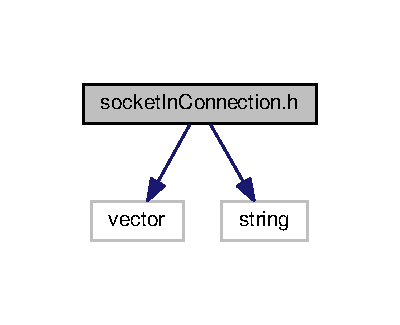
\includegraphics[width=192pt]{d7/df7/KinovaHMICartesianControl_2socketInConnection_8h__incl}
\end{center}
\end{figure}
This graph shows which files directly or indirectly include this file\+:
\nopagebreak
\begin{figure}[H]
\begin{center}
\leavevmode
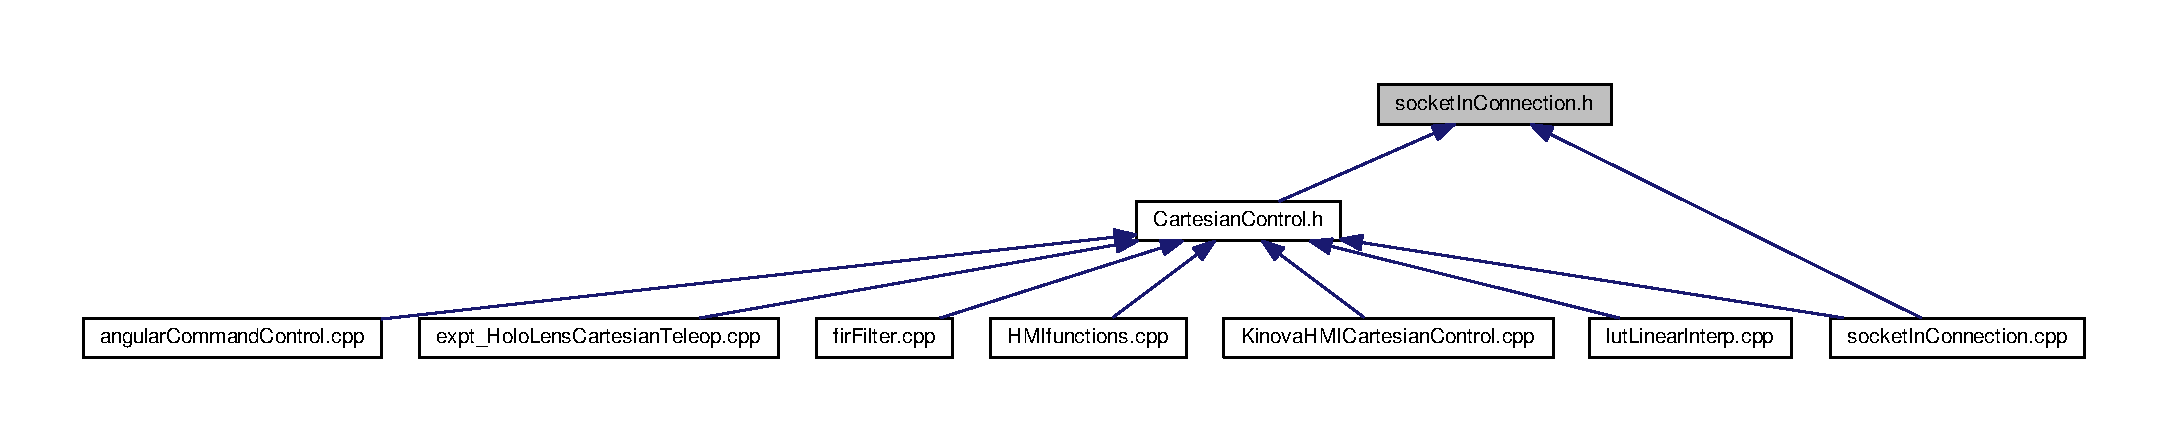
\includegraphics[width=350pt]{d3/dc2/KinovaHMICartesianControl_2socketInConnection_8h__dep__incl}
\end{center}
\end{figure}
\subsection*{Classes}
\begin{DoxyCompactItemize}
\item 
class \hyperlink{classCSocketInConnection}{C\+Socket\+In\+Connection}
\end{DoxyCompactItemize}

\hypertarget{socketInConnection_8h}{}\section{socket\+In\+Connection.\+h File Reference}
\label{socketInConnection_8h}\index{socket\+In\+Connection.\+h@{socket\+In\+Connection.\+h}}
{\ttfamily \#include $<$vector$>$}\\*
{\ttfamily \#include $<$string$>$}\\*
Include dependency graph for socket\+In\+Connection.\+h\+:\nopagebreak
\begin{figure}[H]
\begin{center}
\leavevmode
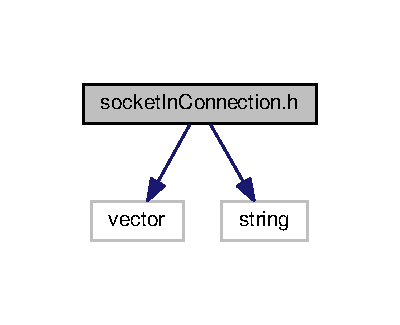
\includegraphics[width=192pt]{da/d1a/socketInConnection_8h__incl}
\end{center}
\end{figure}
This graph shows which files directly or indirectly include this file\+:\nopagebreak
\begin{figure}[H]
\begin{center}
\leavevmode
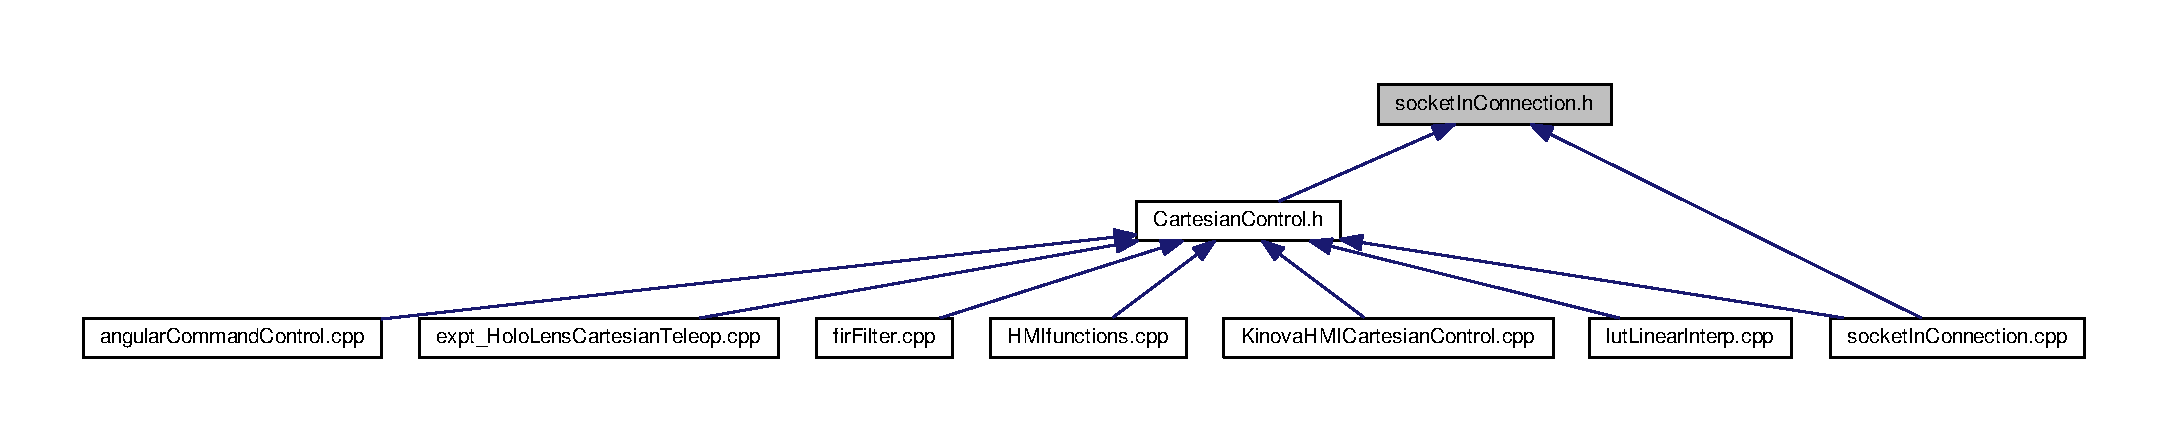
\includegraphics[width=350pt]{d2/d93/socketInConnection_8h__dep__incl}
\end{center}
\end{figure}
\subsection*{Classes}
\begin{DoxyCompactItemize}
\item 
class \hyperlink{classCSocketInConnection}{C\+Socket\+In\+Connection}
\end{DoxyCompactItemize}

\hypertarget{KinovaHMICartesianControl_2socketOutConnection_8h}{}\section{socket\+Out\+Connection.\+h File Reference}
\label{KinovaHMICartesianControl_2socketOutConnection_8h}\index{socket\+Out\+Connection.\+h@{socket\+Out\+Connection.\+h}}
{\ttfamily \#include $<$vector$>$}\\*
{\ttfamily \#include $<$string$>$}\\*
Include dependency graph for Kinova\+H\+M\+I\+Cartesian\+Control/socket\+Out\+Connection.h\+:
\nopagebreak
\begin{figure}[H]
\begin{center}
\leavevmode
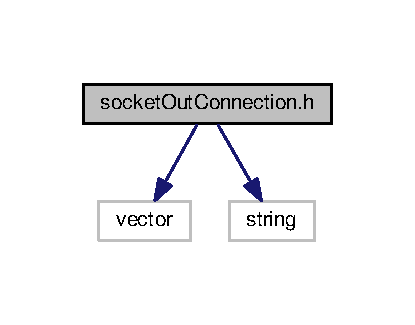
\includegraphics[width=199pt]{dd/db5/KinovaHMICartesianControl_2socketOutConnection_8h__incl}
\end{center}
\end{figure}
\subsection*{Classes}
\begin{DoxyCompactItemize}
\item 
class \hyperlink{classCSocketOutConnection}{C\+Socket\+Out\+Connection}
\end{DoxyCompactItemize}

\hypertarget{socketOutConnection_8h}{}\section{socket\+Out\+Connection.\+h File Reference}
\label{socketOutConnection_8h}\index{socket\+Out\+Connection.\+h@{socket\+Out\+Connection.\+h}}
{\ttfamily \#include $<$vector$>$}\\*
{\ttfamily \#include $<$string$>$}\\*
Include dependency graph for socket\+Out\+Connection.\+h\+:\nopagebreak
\begin{figure}[H]
\begin{center}
\leavevmode
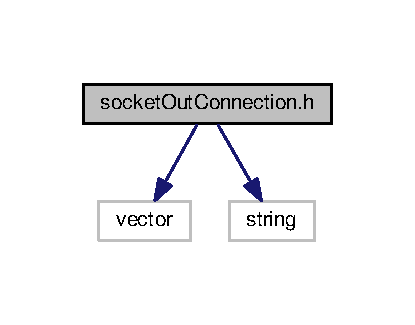
\includegraphics[width=199pt]{df/d2e/socketOutConnection_8h__incl}
\end{center}
\end{figure}
\subsection*{Classes}
\begin{DoxyCompactItemize}
\item 
class \hyperlink{classCSocketOutConnection}{C\+Socket\+Out\+Connection}
\end{DoxyCompactItemize}

\hypertarget{KinovaHMICartesianControl_2stdafx_8cpp}{}\section{stdafx.\+cpp File Reference}
\label{KinovaHMICartesianControl_2stdafx_8cpp}\index{stdafx.\+cpp@{stdafx.\+cpp}}
{\ttfamily \#include \char`\"{}stdafx.\+h\char`\"{}}\\*
Include dependency graph for Kinova\+H\+M\+I\+Cartesian\+Control/stdafx.cpp\+:
\nopagebreak
\begin{figure}[H]
\begin{center}
\leavevmode
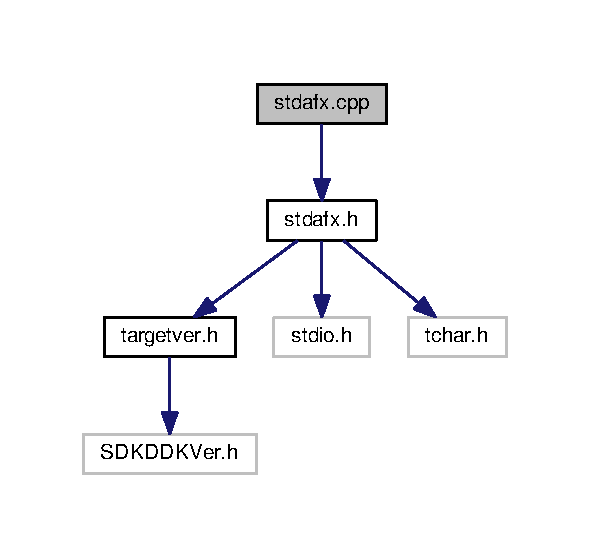
\includegraphics[width=283pt]{df/db4/KinovaHMICartesianControl_2stdafx_8cpp__incl}
\end{center}
\end{figure}

\hypertarget{stdafx_8cpp}{}\section{stdafx.\+cpp File Reference}
\label{stdafx_8cpp}\index{stdafx.\+cpp@{stdafx.\+cpp}}
{\ttfamily \#include \char`\"{}stdafx.\+h\char`\"{}}\\*
Include dependency graph for stdafx.\+cpp\+:\nopagebreak
\begin{figure}[H]
\begin{center}
\leavevmode
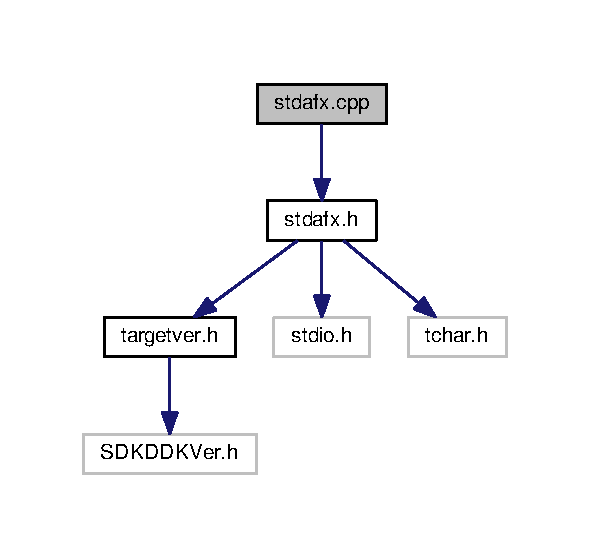
\includegraphics[width=283pt]{de/d79/stdafx_8cpp__incl}
\end{center}
\end{figure}

\hypertarget{KinovaHMICartesianControl_2stdafx_8h}{}\section{stdafx.\+h File Reference}
\label{KinovaHMICartesianControl_2stdafx_8h}\index{stdafx.\+h@{stdafx.\+h}}
{\ttfamily \#include \char`\"{}targetver.\+h\char`\"{}}\\*
{\ttfamily \#include $<$stdio.\+h$>$}\\*
{\ttfamily \#include $<$tchar.\+h$>$}\\*
Include dependency graph for Kinova\+H\+M\+I\+Cartesian\+Control/stdafx.h\+:
\nopagebreak
\begin{figure}[H]
\begin{center}
\leavevmode
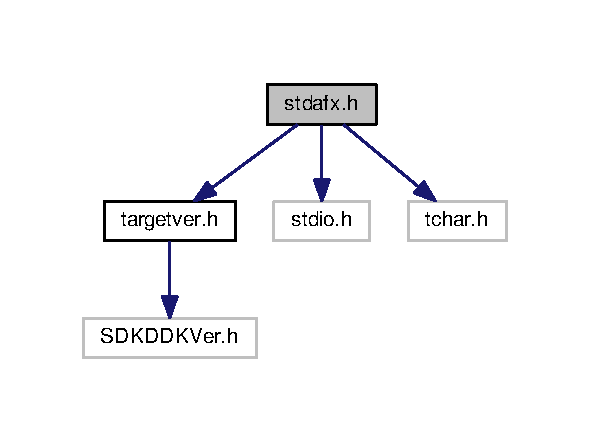
\includegraphics[width=283pt]{dd/dc7/KinovaHMICartesianControl_2stdafx_8h__incl}
\end{center}
\end{figure}
This graph shows which files directly or indirectly include this file\+:
\nopagebreak
\begin{figure}[H]
\begin{center}
\leavevmode
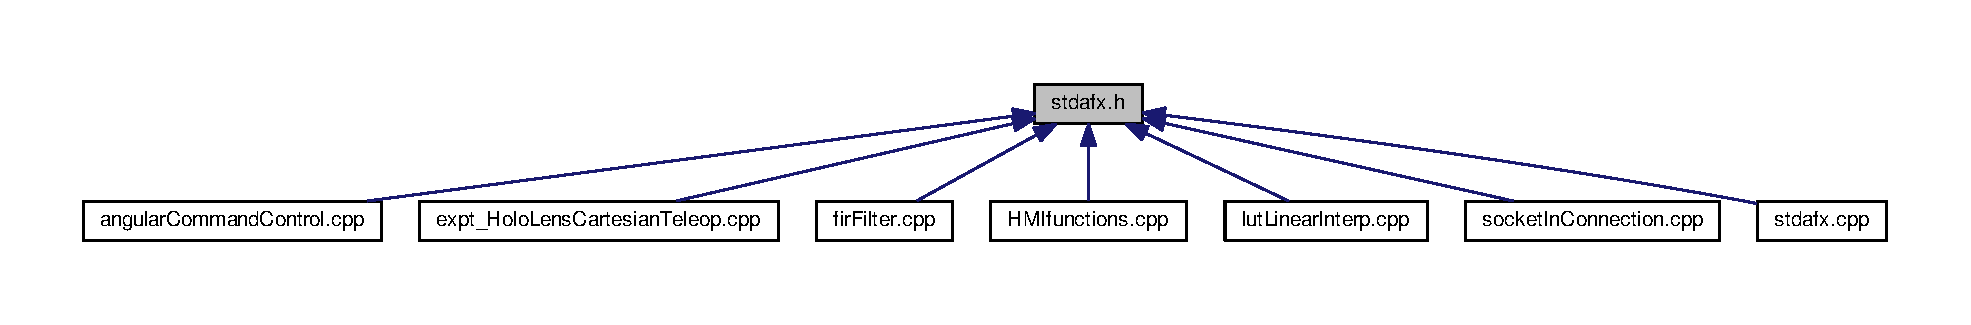
\includegraphics[width=350pt]{d0/dd7/KinovaHMICartesianControl_2stdafx_8h__dep__incl}
\end{center}
\end{figure}

\hypertarget{stdafx_8h}{}\section{stdafx.\+h File Reference}
\label{stdafx_8h}\index{stdafx.\+h@{stdafx.\+h}}
{\ttfamily \#include \char`\"{}targetver.\+h\char`\"{}}\\*
{\ttfamily \#include $<$stdio.\+h$>$}\\*
{\ttfamily \#include $<$tchar.\+h$>$}\\*
Include dependency graph for stdafx.\+h\+:\nopagebreak
\begin{figure}[H]
\begin{center}
\leavevmode
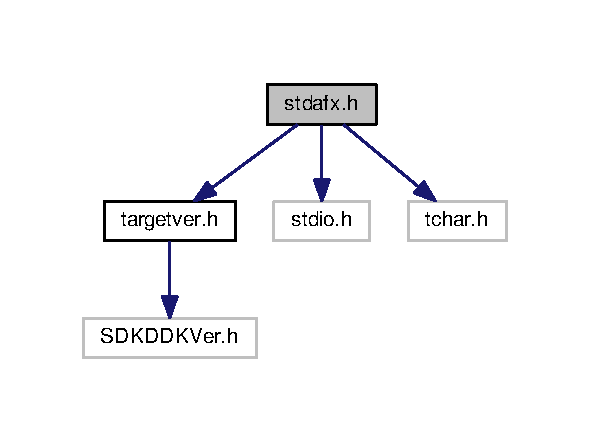
\includegraphics[width=283pt]{d5/da1/stdafx_8h__incl}
\end{center}
\end{figure}
This graph shows which files directly or indirectly include this file\+:\nopagebreak
\begin{figure}[H]
\begin{center}
\leavevmode
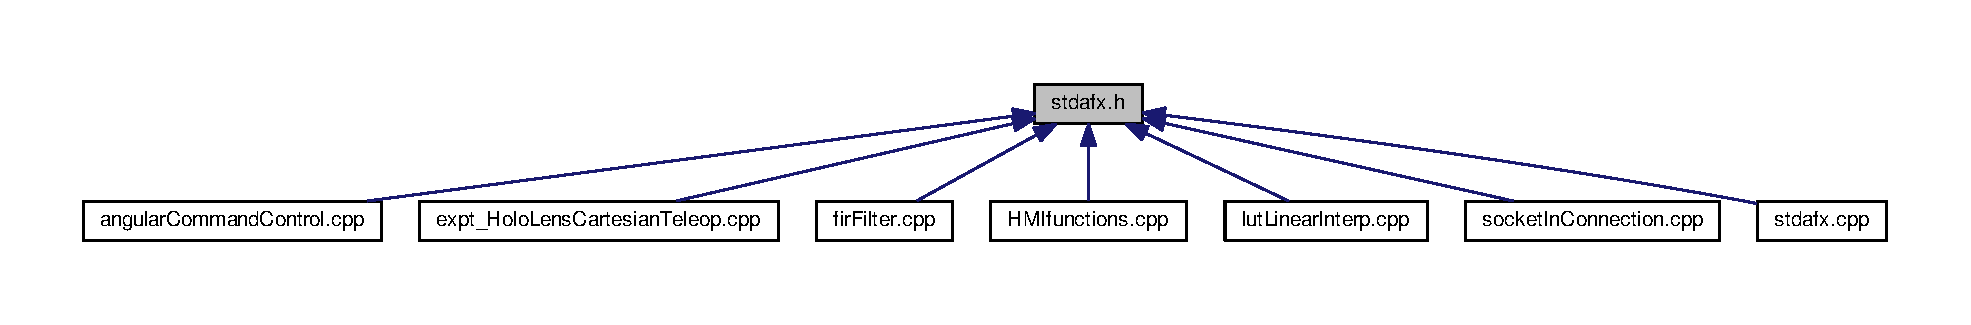
\includegraphics[width=350pt]{d3/d1b/stdafx_8h__dep__incl}
\end{center}
\end{figure}

\hypertarget{KinovaHMICartesianControl_2targetver_8h}{}\section{targetver.\+h File Reference}
\label{KinovaHMICartesianControl_2targetver_8h}\index{targetver.\+h@{targetver.\+h}}
{\ttfamily \#include $<$S\+D\+K\+D\+D\+K\+Ver.\+h$>$}\\*
Include dependency graph for Kinova\+H\+M\+I\+Cartesian\+Control/targetver.h\+:
\nopagebreak
\begin{figure}[H]
\begin{center}
\leavevmode
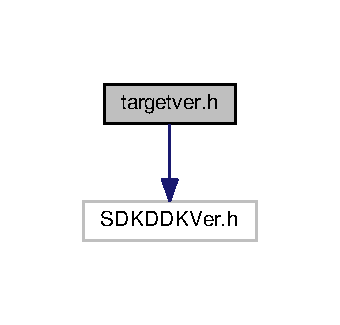
\includegraphics[width=163pt]{df/d22/KinovaHMICartesianControl_2targetver_8h__incl}
\end{center}
\end{figure}
This graph shows which files directly or indirectly include this file\+:
\nopagebreak
\begin{figure}[H]
\begin{center}
\leavevmode
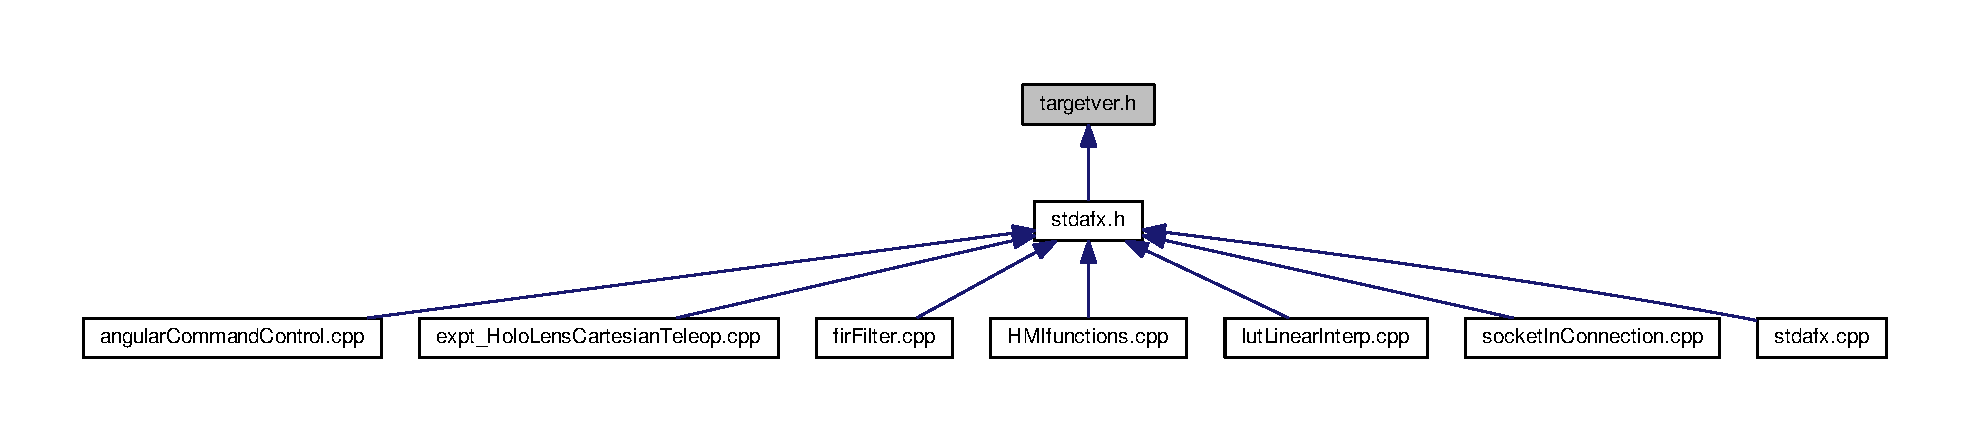
\includegraphics[width=350pt]{de/dcb/KinovaHMICartesianControl_2targetver_8h__dep__incl}
\end{center}
\end{figure}

\hypertarget{targetver_8h}{}\section{targetver.\+h File Reference}
\label{targetver_8h}\index{targetver.\+h@{targetver.\+h}}
{\ttfamily \#include $<$S\+D\+K\+D\+D\+K\+Ver.\+h$>$}\\*
Include dependency graph for targetver.\+h\+:\nopagebreak
\begin{figure}[H]
\begin{center}
\leavevmode
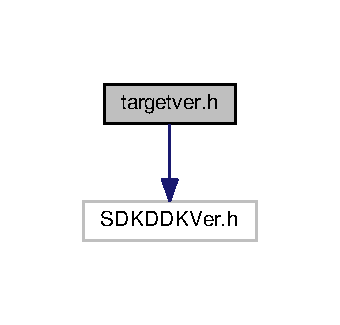
\includegraphics[width=163pt]{d4/dfa/targetver_8h__incl}
\end{center}
\end{figure}
This graph shows which files directly or indirectly include this file\+:\nopagebreak
\begin{figure}[H]
\begin{center}
\leavevmode
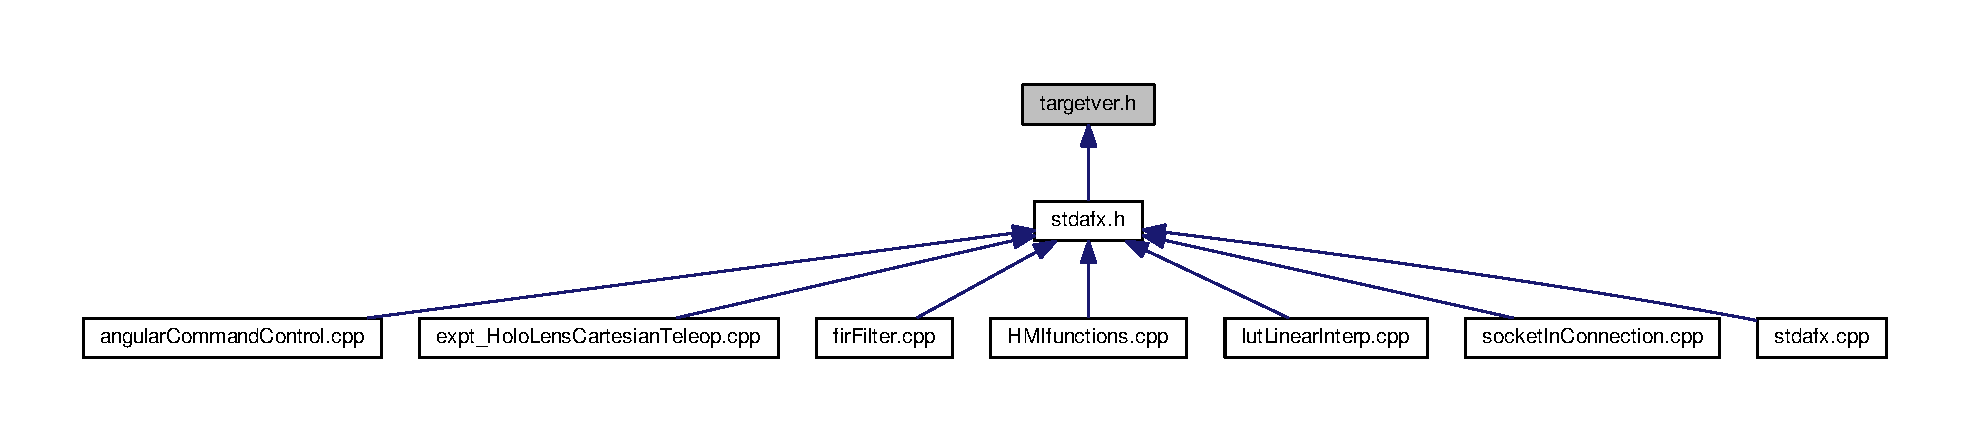
\includegraphics[width=350pt]{dc/dce/targetver_8h__dep__incl}
\end{center}
\end{figure}

\hypertarget{variables__0_8js}{}\section{variables\+\_\+0.\+js File Reference}
\label{variables__0_8js}\index{variables\+\_\+0.\+js@{variables\+\_\+0.\+js}}
\subsection*{Variables}
\begin{DoxyCompactItemize}
\item 
var \hyperlink{variables__0_8js_ad01a7523f103d6242ef9b0451861231e}{search\+Data}
\end{DoxyCompactItemize}


\subsection{Variable Documentation}
\index{variables\+\_\+0.\+js@{variables\+\_\+0.\+js}!search\+Data@{search\+Data}}
\index{search\+Data@{search\+Data}!variables\+\_\+0.\+js@{variables\+\_\+0.\+js}}
\subsubsection[{\texorpdfstring{search\+Data}{searchData}}]{\setlength{\rightskip}{0pt plus 5cm}var search\+Data}\hypertarget{variables__0_8js_ad01a7523f103d6242ef9b0451861231e}{}\label{variables__0_8js_ad01a7523f103d6242ef9b0451861231e}
{\bfseries Initial value\+:}
\begin{DoxyCode}
=
[
  [\textcolor{stringliteral}{'\_5fheaderbyte1'},[\textcolor{stringliteral}{'\_headerByte1'},[\textcolor{stringliteral}{'
      ../d9/d41/classCSocketInConnection.html#a29aaed85ddeae77c458e55a525913f92'},1,\textcolor{stringliteral}{'CSocketInConnection::\_headerByte1()'}],[\textcolor{stringliteral}{'
      ../de/db2/classCSocketOutConnection.html#a35064c765760c0088efc66089090bf2c'},1,\textcolor{stringliteral}{'CSocketOutConnection::\_headerByte1()'}]]],
  [\textcolor{stringliteral}{'\_5fheaderbyte2'},[\textcolor{stringliteral}{'\_headerByte2'},[\textcolor{stringliteral}{'
      ../d9/d41/classCSocketInConnection.html#aba9547facc04cc1229bcf4180665a245'},1,\textcolor{stringliteral}{'CSocketInConnection::\_headerByte2()'}],[\textcolor{stringliteral}{'
      ../de/db2/classCSocketOutConnection.html#a47f6cf4d96b6a829190e37067c6e17f0'},1,\textcolor{stringliteral}{'CSocketOutConnection::\_headerByte2()'}]]],
  [\textcolor{stringliteral}{'\_5fmaxpacketsize'},[\textcolor{stringliteral}{'\_maxPacketSize'},[\textcolor{stringliteral}{'
      ../d9/d41/classCSocketInConnection.html#a7b957c558cb8fe7bbc0d38e7eb935fdd'},1,\textcolor{stringliteral}{'CSocketInConnection::\_maxPacketSize()'}],[\textcolor{stringliteral}{'
      ../de/db2/classCSocketOutConnection.html#a4df79b453417a21cd75b94d639410501'},1,\textcolor{stringliteral}{'CSocketOutConnection::\_maxPacketSize()'}]]],
  [\textcolor{stringliteral}{'\_5fsocketclient'},[\textcolor{stringliteral}{'\_socketClient'},[\textcolor{stringliteral}{'
      ../d9/d41/classCSocketInConnection.html#a56e7bb3cec18ed99eba6edbe8f80141b'},1,\textcolor{stringliteral}{'CSocketInConnection'}]]],
  [\textcolor{stringliteral}{'\_5fsocketconn'},[\textcolor{stringliteral}{'\_socketConn'},[\textcolor{stringliteral}{'
      ../de/db2/classCSocketOutConnection.html#a99dd605a5c9c6f635038213610447ac8'},1,\textcolor{stringliteral}{'CSocketOutConnection'}]]],
  [\textcolor{stringliteral}{'\_5fsocketconnectedmachineip'},[\textcolor{stringliteral}{'\_socketConnectedMachineIP'},[\textcolor{stringliteral}{'
      ../d9/d41/classCSocketInConnection.html#a038af4cdb71b67aa89d459783c03da45'},1,\textcolor{stringliteral}{'CSocketInConnection'}]]],
  [\textcolor{stringliteral}{'\_5fsocketconnectionaddress'},[\textcolor{stringliteral}{'\_socketConnectionAddress'},[\textcolor{stringliteral}{'
      ../de/db2/classCSocketOutConnection.html#a84876c61143ce6ebf83082824ca1d232'},1,\textcolor{stringliteral}{'CSocketOutConnection'}]]],
  [\textcolor{stringliteral}{'\_5fsocketconnectionport'},[\textcolor{stringliteral}{'\_socketConnectionPort'},[\textcolor{stringliteral}{'
      ../d9/d41/classCSocketInConnection.html#a4a51213ec51b9d4e51c7006828f988fb'},1,\textcolor{stringliteral}{'CSocketInConnection::\_socketConnectionPort()'}],[\textcolor{stringliteral}{'
      ../de/db2/classCSocketOutConnection.html#a760902b8101aca205a3556020bc7bc50'},1,\textcolor{stringliteral}{'CSocketOutConnection::\_socketConnectionPort()'}]]],
  [\textcolor{stringliteral}{'\_5fsocketconnectwasok'},[\textcolor{stringliteral}{'\_socketConnectWasOk'},[\textcolor{stringliteral}{'
      ../d9/d41/classCSocketInConnection.html#a01ce97069b2749c8921bc2f043086de1'},1,\textcolor{stringliteral}{'CSocketInConnection'}]]],
  [\textcolor{stringliteral}{'\_5fsocketlocal'},[\textcolor{stringliteral}{'\_socketLocal'},[\textcolor{stringliteral}{'
      ../d9/d41/classCSocketInConnection.html#a7fbfa7dd8415d8cd50ddc3062bc2c1c8'},1,\textcolor{stringliteral}{'CSocketInConnection'}]]],
  [\textcolor{stringliteral}{'\_5fsocketserver'},[\textcolor{stringliteral}{'\_socketServer'},[\textcolor{stringliteral}{'
      ../d9/d41/classCSocketInConnection.html#aee8c491e5d179aa20921f38cef08ac0d'},1,\textcolor{stringliteral}{'CSocketInConnection::\_socketServer()'}],[\textcolor{stringliteral}{'
      ../de/db2/classCSocketOutConnection.html#a7a4a2efbc8fced507bd76b88c2725af3'},1,\textcolor{stringliteral}{'CSocketOutConnection::\_socketServer()'}]]],
  [\textcolor{stringliteral}{'\_5fsockettheset'},[\textcolor{stringliteral}{'\_socketTheSet'},[\textcolor{stringliteral}{'
      ../d9/d41/classCSocketInConnection.html#a0d6c6fbb3215d3ba3332fca268802d44'},1,\textcolor{stringliteral}{'CSocketInConnection'}]]]
]
\end{DoxyCode}

\hypertarget{variables__1_8js}{}\section{variables\+\_\+1.\+js File Reference}
\label{variables__1_8js}\index{variables\+\_\+1.\+js@{variables\+\_\+1.\+js}}
\subsection*{Variables}
\begin{DoxyCompactItemize}
\item 
var \hyperlink{variables__1_8js_ad01a7523f103d6242ef9b0451861231e}{search\+Data}
\end{DoxyCompactItemize}


\subsection{Variable Documentation}
\index{variables\+\_\+1.\+js@{variables\+\_\+1.\+js}!search\+Data@{search\+Data}}
\index{search\+Data@{search\+Data}!variables\+\_\+1.\+js@{variables\+\_\+1.\+js}}
\subsubsection[{\texorpdfstring{search\+Data}{searchData}}]{\setlength{\rightskip}{0pt plus 5cm}var search\+Data}\hypertarget{variables__1_8js_ad01a7523f103d6242ef9b0451861231e}{}\label{variables__1_8js_ad01a7523f103d6242ef9b0451861231e}
{\bfseries Initial value\+:}
\begin{DoxyCode}
=
[
  [\textcolor{stringliteral}{'angularvelocity'},[\textcolor{stringliteral}{'angularVelocity'},[\textcolor{stringliteral}{'
      ../d6/da6/classNovintFalconHapticsDevice.html#a8f71db7ac35c67569dac444e8ac91bb4'},1,\textcolor{stringliteral}{'NovintFalconHapticsDevice'}]]]
]
\end{DoxyCode}

\hypertarget{variables__10_8js}{}\section{variables\+\_\+10.\+js File Reference}
\label{variables__10_8js}\index{variables\+\_\+10.\+js@{variables\+\_\+10.\+js}}
\subsection*{Variables}
\begin{DoxyCompactItemize}
\item 
var \hyperlink{variables__10_8js_ad01a7523f103d6242ef9b0451861231e}{search\+Data}
\end{DoxyCompactItemize}


\subsection{Variable Documentation}
\index{variables\+\_\+10.\+js@{variables\+\_\+10.\+js}!search\+Data@{search\+Data}}
\index{search\+Data@{search\+Data}!variables\+\_\+10.\+js@{variables\+\_\+10.\+js}}
\subsubsection[{\texorpdfstring{search\+Data}{searchData}}]{\setlength{\rightskip}{0pt plus 5cm}var search\+Data}\hypertarget{variables__10_8js_ad01a7523f103d6242ef9b0451861231e}{}\label{variables__10_8js_ad01a7523f103d6242ef9b0451861231e}
{\bfseries Initial value\+:}
\begin{DoxyCode}
=
[
  [\textcolor{charliteral}{'t'},[\textcolor{charliteral}{'T'},[\textcolor{stringliteral}{'../d8/d06/classExperiment.html#add6f49b3c33cde40d8a6114c45d5475f'},1,\textcolor{stringliteral}{'Experiment'}]]],
  [\textcolor{stringliteral}{'t\_5fcalib'},[\textcolor{stringliteral}{'T\_calib'},[\textcolor{stringliteral}{'../d8/d06/classExperiment.html#a0e11440fb68bc29a305c2757e5c85550'},1,\textcolor{stringliteral}{'Experiment
      '}]]],
  [\textcolor{stringliteral}{'t\_5ftf'},[\textcolor{stringliteral}{'T\_TF'},[\textcolor{stringliteral}{'../d8/d06/classExperiment.html#ae4044c67ccebf1fd2370d304c2b6e6a6'},1,\textcolor{stringliteral}{'Experiment'}]]],
  [\textcolor{stringliteral}{'ts'},[\textcolor{stringliteral}{'Ts'},[\textcolor{stringliteral}{'../d8/d06/classExperiment.html#ac51084a578b7edb7fa68f96d98671609'},1,\textcolor{stringliteral}{'Experiment'}]]]
]
\end{DoxyCode}

\hypertarget{variables__11_8js}{}\section{variables\+\_\+11.\+js File Reference}
\label{variables__11_8js}\index{variables\+\_\+11.\+js@{variables\+\_\+11.\+js}}
\subsection*{Variables}
\begin{DoxyCompactItemize}
\item 
var \hyperlink{variables__11_8js_ad01a7523f103d6242ef9b0451861231e}{search\+Data}
\end{DoxyCompactItemize}


\subsection{Variable Documentation}
\index{variables\+\_\+11.\+js@{variables\+\_\+11.\+js}!search\+Data@{search\+Data}}
\index{search\+Data@{search\+Data}!variables\+\_\+11.\+js@{variables\+\_\+11.\+js}}
\subsubsection[{\texorpdfstring{search\+Data}{searchData}}]{\setlength{\rightskip}{0pt plus 5cm}var search\+Data}\hypertarget{variables__11_8js_ad01a7523f103d6242ef9b0451861231e}{}\label{variables__11_8js_ad01a7523f103d6242ef9b0451861231e}
{\bfseries Initial value\+:}
\begin{DoxyCode}
=
[
  [\textcolor{stringliteral}{'usedamping'},[\textcolor{stringliteral}{'useDamping'},[\textcolor{stringliteral}{'
      ../d6/da6/classNovintFalconHapticsDevice.html#a8343a6b7e8c05449d1fd4daf39f346a9'},1,\textcolor{stringliteral}{'NovintFalconHapticsDevice'}]]],
  [\textcolor{stringliteral}{'useforcefield'},[\textcolor{stringliteral}{'useForceField'},[\textcolor{stringliteral}{'
      ../d6/da6/classNovintFalconHapticsDevice.html#ab057b4217959d896c52fc5167be1314d'},1,\textcolor{stringliteral}{'NovintFalconHapticsDevice'}]]],
  [\textcolor{stringliteral}{'userfound'},[\textcolor{stringliteral}{'userFound'},[\textcolor{stringliteral}{'
      ../da/db1/structkinectSkelTrack\_1\_1KinectInfo.html#a772bf02b53092fd2424849292b2c3c1d'},1,\textcolor{stringliteral}{'kinectSkelTrack::KinectInfo'}]]]
]
\end{DoxyCode}

\hypertarget{variables__12_8js}{}\section{variables\+\_\+12.\+js File Reference}
\label{variables__12_8js}\index{variables\+\_\+12.\+js@{variables\+\_\+12.\+js}}
\subsection*{Variables}
\begin{DoxyCompactItemize}
\item 
var \hyperlink{variables__12_8js_ad01a7523f103d6242ef9b0451861231e}{search\+Data}
\end{DoxyCompactItemize}


\subsection{Variable Documentation}
\index{variables\+\_\+12.\+js@{variables\+\_\+12.\+js}!search\+Data@{search\+Data}}
\index{search\+Data@{search\+Data}!variables\+\_\+12.\+js@{variables\+\_\+12.\+js}}
\subsubsection[{\texorpdfstring{search\+Data}{searchData}}]{\setlength{\rightskip}{0pt plus 5cm}var search\+Data}\hypertarget{variables__12_8js_ad01a7523f103d6242ef9b0451861231e}{}\label{variables__12_8js_ad01a7523f103d6242ef9b0451861231e}
{\bfseries Initial value\+:}
\begin{DoxyCode}
=
[
  [\textcolor{stringliteral}{'width'},[\textcolor{stringliteral}{'width'},[\textcolor{stringliteral}{'../d0/d05/classkinectSkelTrack.html#a8f20f39c8822eecba07518a8b35a9f2b'},1,\textcolor{stringliteral}{'
      kinectSkelTrack'}]]]
]
\end{DoxyCode}

\hypertarget{variables__2_8js}{}\section{variables\+\_\+2.\+js File Reference}
\label{variables__2_8js}\index{variables\+\_\+2.\+js@{variables\+\_\+2.\+js}}
\subsection*{Variables}
\begin{DoxyCompactItemize}
\item 
var \hyperlink{variables__2_8js_ad01a7523f103d6242ef9b0451861231e}{search\+Data}
\end{DoxyCompactItemize}


\subsection{Variable Documentation}
\index{variables\+\_\+2.\+js@{variables\+\_\+2.\+js}!search\+Data@{search\+Data}}
\index{search\+Data@{search\+Data}!variables\+\_\+2.\+js@{variables\+\_\+2.\+js}}
\subsubsection[{\texorpdfstring{search\+Data}{searchData}}]{\setlength{\rightskip}{0pt plus 5cm}var search\+Data}\hypertarget{variables__2_8js_ad01a7523f103d6242ef9b0451861231e}{}\label{variables__2_8js_ad01a7523f103d6242ef9b0451861231e}
{\bfseries Initial value\+:}
\begin{DoxyCode}
=
[
  [\textcolor{stringliteral}{'button0\_5fstate'},[\textcolor{stringliteral}{'button0\_state'},[\textcolor{stringliteral}{'
      ../d6/da6/classNovintFalconHapticsDevice.html#addebfcfc98d7e5593e369beea025e1bf'},1,\textcolor{stringliteral}{'NovintFalconHapticsDevice'}]]],
  [\textcolor{stringliteral}{'button2\_5fstate'},[\textcolor{stringliteral}{'button2\_state'},[\textcolor{stringliteral}{'
      ../d6/da6/classNovintFalconHapticsDevice.html#af016391ef02d82857ad1e65bf32faaa3'},1,\textcolor{stringliteral}{'NovintFalconHapticsDevice'}]]]
]
\end{DoxyCode}

\hypertarget{variables__3_8js}{}\section{variables\+\_\+3.\+js File Reference}
\label{variables__3_8js}\index{variables\+\_\+3.\+js@{variables\+\_\+3.\+js}}
\subsection*{Variables}
\begin{DoxyCompactItemize}
\item 
var \hyperlink{variables__3_8js_ad01a7523f103d6242ef9b0451861231e}{search\+Data}
\end{DoxyCompactItemize}


\subsection{Variable Documentation}
\index{variables\+\_\+3.\+js@{variables\+\_\+3.\+js}!search\+Data@{search\+Data}}
\index{search\+Data@{search\+Data}!variables\+\_\+3.\+js@{variables\+\_\+3.\+js}}
\subsubsection[{\texorpdfstring{search\+Data}{searchData}}]{\setlength{\rightskip}{0pt plus 5cm}var search\+Data}\hypertarget{variables__3_8js_ad01a7523f103d6242ef9b0451861231e}{}\label{variables__3_8js_ad01a7523f103d6242ef9b0451861231e}
{\bfseries Initial value\+:}
\begin{DoxyCode}
=
[
  [\textcolor{stringliteral}{'coeffs'},[\textcolor{stringliteral}{'coeffs'},[\textcolor{stringliteral}{'../d3/d32/classFIRFilter.html#a52132dfc0390a6124ecd557f77d87084'},1,\textcolor{stringliteral}{'FIRFilter'}]]],
  [\textcolor{stringliteral}{'commandlayer\_5fhandle'},[\textcolor{stringliteral}{'commandLayer\_handle'},[\textcolor{stringliteral}{'
      ../d0/da0/KinovaHMICartesianControl\_8cpp.html#a7dcbafc298af1cba5defa0baf9cfb948'},1,\textcolor{stringliteral}{'KinovaHMICartesianControl.cpp'}]]],
  [\textcolor{stringliteral}{'cutoff\_5ffreq\_5fhz'},[\textcolor{stringliteral}{'cutoff\_freq\_hz'},[\textcolor{stringliteral}{'../d3/d32/classFIRFilter.html#a038a40d113cdbcdef9d215f79d5e22bf
      '},1,\textcolor{stringliteral}{'FIRFilter'}]]]
]
\end{DoxyCode}

\hypertarget{variables__4_8js}{}\section{variables\+\_\+4.\+js File Reference}
\label{variables__4_8js}\index{variables\+\_\+4.\+js@{variables\+\_\+4.\+js}}
\subsection*{Variables}
\begin{DoxyCompactItemize}
\item 
var \hyperlink{variables__4_8js_ad01a7523f103d6242ef9b0451861231e}{search\+Data}
\end{DoxyCompactItemize}


\subsection{Variable Documentation}
\index{variables\+\_\+4.\+js@{variables\+\_\+4.\+js}!search\+Data@{search\+Data}}
\index{search\+Data@{search\+Data}!variables\+\_\+4.\+js@{variables\+\_\+4.\+js}}
\subsubsection[{\texorpdfstring{search\+Data}{searchData}}]{\setlength{\rightskip}{0pt plus 5cm}var search\+Data}\hypertarget{variables__4_8js_ad01a7523f103d6242ef9b0451861231e}{}\label{variables__4_8js_ad01a7523f103d6242ef9b0451861231e}
{\bfseries Initial value\+:}
\begin{DoxyCode}
=
[
  [\textcolor{stringliteral}{'depthstream'},[\textcolor{stringliteral}{'depthStream'},[\textcolor{stringliteral}{'../d0/d05/classkinectSkelTrack.html#ac736221c582bd751c18af867bd1b90f1'},1,\textcolor{stringliteral}{
      'kinectSkelTrack'}]]],
  [\textcolor{stringliteral}{'desiredposition'},[\textcolor{stringliteral}{'desiredPosition'},[\textcolor{stringliteral}{'
      ../d6/da6/classNovintFalconHapticsDevice.html#afcd63a3be7d519dd7f983414f9e0f24c'},1,\textcolor{stringliteral}{'NovintFalconHapticsDevice'}]]],
  [\textcolor{stringliteral}{'desiredrotation'},[\textcolor{stringliteral}{'desiredRotation'},[\textcolor{stringliteral}{'
      ../d6/da6/classNovintFalconHapticsDevice.html#acb82e8e4273b4979aae7cba6989058b6'},1,\textcolor{stringliteral}{'NovintFalconHapticsDevice'}]]]
]
\end{DoxyCode}

\hypertarget{variables__5_8js}{}\section{variables\+\_\+5.\+js File Reference}
\label{variables__5_8js}\index{variables\+\_\+5.\+js@{variables\+\_\+5.\+js}}
\subsection*{Variables}
\begin{DoxyCompactItemize}
\item 
var \hyperlink{variables__5_8js_ad01a7523f103d6242ef9b0451861231e}{search\+Data}
\end{DoxyCompactItemize}


\subsection{Variable Documentation}
\index{variables\+\_\+5.\+js@{variables\+\_\+5.\+js}!search\+Data@{search\+Data}}
\index{search\+Data@{search\+Data}!variables\+\_\+5.\+js@{variables\+\_\+5.\+js}}
\subsubsection[{\texorpdfstring{search\+Data}{searchData}}]{\setlength{\rightskip}{0pt plus 5cm}var search\+Data}\hypertarget{variables__5_8js_ad01a7523f103d6242ef9b0451861231e}{}\label{variables__5_8js_ad01a7523f103d6242ef9b0451861231e}
{\bfseries Initial value\+:}
\begin{DoxyCode}
=
[
  [\textcolor{stringliteral}{'filename'},[\textcolor{stringliteral}{'filename'},[\textcolor{stringliteral}{'../d3/d32/classFIRFilter.html#af15d0e43051eb388273fe4b575e7e791'},1,\textcolor{stringliteral}{'FIRFilter'}]
      ]],
  [\textcolor{stringliteral}{'fs\_5fqd\_5flut'},[\textcolor{stringliteral}{'fs\_qd\_lut'},[\textcolor{stringliteral}{'../d8/d06/classExperiment.html#a04ef11e89995e42aee1b89d5bba35aae'},1,\textcolor{stringliteral}{'
      Experiment'}]]],
  [\textcolor{stringliteral}{'fs\_5fuc\_5flut'},[\textcolor{stringliteral}{'fs\_uc\_lut'},[\textcolor{stringliteral}{'../d8/d06/classExperiment.html#a64ab0761b30b073656aa75760d2e230d'},1,\textcolor{stringliteral}{'
      Experiment'}]]]
]
\end{DoxyCode}

\hypertarget{variables__6_8js}{}\section{variables\+\_\+6.\+js File Reference}
\label{variables__6_8js}\index{variables\+\_\+6.\+js@{variables\+\_\+6.\+js}}
\subsection*{Variables}
\begin{DoxyCompactItemize}
\item 
var \hyperlink{variables__6_8js_ad01a7523f103d6242ef9b0451861231e}{search\+Data}
\end{DoxyCompactItemize}


\subsection{Variable Documentation}
\index{variables\+\_\+6.\+js@{variables\+\_\+6.\+js}!search\+Data@{search\+Data}}
\index{search\+Data@{search\+Data}!variables\+\_\+6.\+js@{variables\+\_\+6.\+js}}
\subsubsection[{\texorpdfstring{search\+Data}{searchData}}]{\setlength{\rightskip}{0pt plus 5cm}var search\+Data}\hypertarget{variables__6_8js_ad01a7523f103d6242ef9b0451861231e}{}\label{variables__6_8js_ad01a7523f103d6242ef9b0451861231e}
{\bfseries Initial value\+:}
\begin{DoxyCode}
=
[
  [\textcolor{stringliteral}{'handler'},[\textcolor{stringliteral}{'handler'},[\textcolor{stringliteral}{'../d6/da6/classNovintFalconHapticsDevice.html#a64bca002d3939aede4ecbabbe2613865'},
      1,\textcolor{stringliteral}{'NovintFalconHapticsDevice'}]]],
  [\textcolor{stringliteral}{'handposition'},[\textcolor{stringliteral}{'handPosition'},[\textcolor{stringliteral}{'
      ../da/db1/structkinectSkelTrack\_1\_1KinectInfo.html#a22f3400cf45556b243dcf94bcf4392df'},1,\textcolor{stringliteral}{'kinectSkelTrack::KinectInfo'}]]],
  [\textcolor{stringliteral}{'hapticdevice'},[\textcolor{stringliteral}{'hapticDevice'},[\textcolor{stringliteral}{'
      ../d6/da6/classNovintFalconHapticsDevice.html#aa5184bbe68246d129003f66c3d5a9628'},1,\textcolor{stringliteral}{'NovintFalconHapticsDevice'}]]],
  [\textcolor{stringliteral}{'hapticdeviceposition'},[\textcolor{stringliteral}{'hapticDevicePosition'},[\textcolor{stringliteral}{'
      ../d6/da6/classNovintFalconHapticsDevice.html#a7815111e1968006b1a6848c040e0e310'},1,\textcolor{stringliteral}{'NovintFalconHapticsDevice'}]]],
  [\textcolor{stringliteral}{'hapticsthread'},[\textcolor{stringliteral}{'hapticsThread'},[\textcolor{stringliteral}{'
      ../d6/da6/classNovintFalconHapticsDevice.html#a7257d16146ffc12eed6044a7321b7397'},1,\textcolor{stringliteral}{'NovintFalconHapticsDevice'}]]],
  [\textcolor{stringliteral}{'height'},[\textcolor{stringliteral}{'height'},[\textcolor{stringliteral}{'../d0/d05/classkinectSkelTrack.html#a028f14282cd4301c8527703300d3dfe8'},1,\textcolor{stringliteral}{'
      kinectSkelTrack'}]]]
]
\end{DoxyCode}

\hypertarget{variables__7_8js}{}\section{variables\+\_\+7.\+js File Reference}
\label{variables__7_8js}\index{variables\+\_\+7.\+js@{variables\+\_\+7.\+js}}
\subsection*{Variables}
\begin{DoxyCompactItemize}
\item 
var \hyperlink{variables__7_8js_ad01a7523f103d6242ef9b0451861231e}{search\+Data}
\end{DoxyCompactItemize}


\subsection{Variable Documentation}
\index{variables\+\_\+7.\+js@{variables\+\_\+7.\+js}!search\+Data@{search\+Data}}
\index{search\+Data@{search\+Data}!variables\+\_\+7.\+js@{variables\+\_\+7.\+js}}
\subsubsection[{\texorpdfstring{search\+Data}{searchData}}]{\setlength{\rightskip}{0pt plus 5cm}var search\+Data}\hypertarget{variables__7_8js_ad01a7523f103d6242ef9b0451861231e}{}\label{variables__7_8js_ad01a7523f103d6242ef9b0451861231e}
{\bfseries Initial value\+:}
\begin{DoxyCode}
=
[
  [\textcolor{stringliteral}{'insamp'},[\textcolor{stringliteral}{'insamp'},[\textcolor{stringliteral}{'../d3/d32/classFIRFilter.html#a3998b6c0cda5c66c708238ee679c415e'},1,\textcolor{stringliteral}{'FIRFilter'}]]],
  [\textcolor{stringliteral}{'isrunning'},[\textcolor{stringliteral}{'isRunning'},[\textcolor{stringliteral}{'
      ../d6/da6/classNovintFalconHapticsDevice.html#afa3018d647b1096332fc0076b9b70733'},1,\textcolor{stringliteral}{'NovintFalconHapticsDevice'}]]]
]
\end{DoxyCode}

\hypertarget{variables__8_8js}{}\section{variables\+\_\+8.\+js File Reference}
\label{variables__8_8js}\index{variables\+\_\+8.\+js@{variables\+\_\+8.\+js}}
\subsection*{Variables}
\begin{DoxyCompactItemize}
\item 
var \hyperlink{variables__8_8js_ad01a7523f103d6242ef9b0451861231e}{search\+Data}
\end{DoxyCompactItemize}


\subsection{Variable Documentation}
\index{variables\+\_\+8.\+js@{variables\+\_\+8.\+js}!search\+Data@{search\+Data}}
\index{search\+Data@{search\+Data}!variables\+\_\+8.\+js@{variables\+\_\+8.\+js}}
\subsubsection[{\texorpdfstring{search\+Data}{searchData}}]{\setlength{\rightskip}{0pt plus 5cm}var search\+Data}\hypertarget{variables__8_8js_ad01a7523f103d6242ef9b0451861231e}{}\label{variables__8_8js_ad01a7523f103d6242ef9b0451861231e}
{\bfseries Initial value\+:}
\begin{DoxyCode}
=
[
  [\textcolor{stringliteral}{'kp'},[\textcolor{stringliteral}{'Kp'},[\textcolor{stringliteral}{'../d8/d06/classExperiment.html#a03450b58564f4dbecb58e773e1cf5e8b'},1,\textcolor{stringliteral}{'Experiment'}]]]
]
\end{DoxyCode}

\hypertarget{variables__9_8js}{}\section{variables\+\_\+9.\+js File Reference}
\label{variables__9_8js}\index{variables\+\_\+9.\+js@{variables\+\_\+9.\+js}}
\subsection*{Variables}
\begin{DoxyCompactItemize}
\item 
var \hyperlink{variables__9_8js_ad01a7523f103d6242ef9b0451861231e}{search\+Data}
\end{DoxyCompactItemize}


\subsection{Variable Documentation}
\index{variables\+\_\+9.\+js@{variables\+\_\+9.\+js}!search\+Data@{search\+Data}}
\index{search\+Data@{search\+Data}!variables\+\_\+9.\+js@{variables\+\_\+9.\+js}}
\subsubsection[{\texorpdfstring{search\+Data}{searchData}}]{\setlength{\rightskip}{0pt plus 5cm}var search\+Data}\hypertarget{variables__9_8js_ad01a7523f103d6242ef9b0451861231e}{}\label{variables__9_8js_ad01a7523f103d6242ef9b0451861231e}
{\bfseries Initial value\+:}
\begin{DoxyCode}
=
[
  [\textcolor{stringliteral}{'len\_5flut'},[\textcolor{stringliteral}{'len\_LUT'},[\textcolor{stringliteral}{'../d8/d06/classExperiment.html#af6e1965489695707f8de14f8ee5b09a1'},1,\textcolor{stringliteral}{'Experiment
      '}]]],
  [\textcolor{stringliteral}{'length'},[\textcolor{stringliteral}{'length'},[\textcolor{stringliteral}{'../d3/d32/classFIRFilter.html#a4e697a78993656c942005939a3439b3f'},1,\textcolor{stringliteral}{'FIRFilter'}]]],
  [\textcolor{stringliteral}{'linearvelocity'},[\textcolor{stringliteral}{'linearVelocity'},[\textcolor{stringliteral}{'
      ../d6/da6/classNovintFalconHapticsDevice.html#a59f432627f7b981c9555216997110bcc'},1,\textcolor{stringliteral}{'NovintFalconHapticsDevice'}]]],
  [\textcolor{stringliteral}{'lut'},[\textcolor{stringliteral}{'LUT'},[\textcolor{stringliteral}{'../d8/d06/classExperiment.html#abfa65531d9549c3df64e52a77a93352e'},1,\textcolor{stringliteral}{'Experiment'}]]]
]
\end{DoxyCode}

\hypertarget{variables__a_8js}{}\section{variables\+\_\+a.\+js File Reference}
\label{variables__a_8js}\index{variables\+\_\+a.\+js@{variables\+\_\+a.\+js}}
\subsection*{Variables}
\begin{DoxyCompactItemize}
\item 
var \hyperlink{variables__a_8js_ad01a7523f103d6242ef9b0451861231e}{search\+Data}
\end{DoxyCompactItemize}


\subsection{Variable Documentation}
\index{variables\+\_\+a.\+js@{variables\+\_\+a.\+js}!search\+Data@{search\+Data}}
\index{search\+Data@{search\+Data}!variables\+\_\+a.\+js@{variables\+\_\+a.\+js}}
\subsubsection[{\texorpdfstring{search\+Data}{searchData}}]{\setlength{\rightskip}{0pt plus 5cm}var search\+Data}\hypertarget{variables__a_8js_ad01a7523f103d6242ef9b0451861231e}{}\label{variables__a_8js_ad01a7523f103d6242ef9b0451861231e}
{\bfseries Initial value\+:}
\begin{DoxyCode}
=
[
  [\textcolor{stringliteral}{'maxforce'},[\textcolor{stringliteral}{'maxforce'},[\textcolor{stringliteral}{'../d6/da6/classNovintFalconHapticsDevice.html#a8cdeb18d8b1e6468c6d4d2e3d2f3e55e
      '},1,\textcolor{stringliteral}{'NovintFalconHapticsDevice'}]]],
  [\textcolor{stringliteral}{'mycloseapi'},[\textcolor{stringliteral}{'MyCloseAPI'},[\textcolor{stringliteral}{'../d9/d19/classKinovaAPIFunctions.html#a769e4a4b1ad66aac175818db5d466ab1'},1
      ,\textcolor{stringliteral}{'KinovaAPIFunctions'}]]],
  [\textcolor{stringliteral}{'mygetactualtrajectoryinfo'},[\textcolor{stringliteral}{'MyGetActualTrajectoryInfo'},[\textcolor{stringliteral}{'
      ../d9/d19/classKinovaAPIFunctions.html#a7768fef3a414ed9910b29e07d8cec5ed'},1,\textcolor{stringliteral}{'KinovaAPIFunctions'}]]],
  [\textcolor{stringliteral}{'mygetangularposition'},[\textcolor{stringliteral}{'MyGetAngularPosition'},[\textcolor{stringliteral}{'
      ../d9/d19/classKinovaAPIFunctions.html#aa3b25eca0b164393821019388459015a'},1,\textcolor{stringliteral}{'KinovaAPIFunctions'}]]],
  [\textcolor{stringliteral}{'mygetcartesiancommand'},[\textcolor{stringliteral}{'MyGetCartesianCommand'},[\textcolor{stringliteral}{'
      ../d9/d19/classKinovaAPIFunctions.html#a0306932b326f70ea7bca5903ba0a14f6'},1,\textcolor{stringliteral}{'KinovaAPIFunctions'}]]],
  [\textcolor{stringliteral}{'mygetcartesianposition'},[\textcolor{stringliteral}{'MyGetCartesianPosition'},[\textcolor{stringliteral}{'
      ../d9/d19/classKinovaAPIFunctions.html#ad6a222c864c2f8005093a038138660cc'},1,\textcolor{stringliteral}{'KinovaAPIFunctions'}]]],
  [\textcolor{stringliteral}{'mygetclientconfigurations'},[\textcolor{stringliteral}{'MyGetClientConfigurations'},[\textcolor{stringliteral}{'
      ../d9/d19/classKinovaAPIFunctions.html#a6963b06d9d1a59c04465bda48ff2a5ab'},1,\textcolor{stringliteral}{'KinovaAPIFunctions'}]]],
  [\textcolor{stringliteral}{'mygetdevices'},[\textcolor{stringliteral}{'MyGetDevices'},[\textcolor{stringliteral}{'
      ../d9/d19/classKinovaAPIFunctions.html#a8d0313599ab0d35b7de11113e17b90f2'},1,\textcolor{stringliteral}{'KinovaAPIFunctions'}]]],
  [\textcolor{stringliteral}{'mygetglobaltrajectoryinfo'},[\textcolor{stringliteral}{'MyGetGlobalTrajectoryInfo'},[\textcolor{stringliteral}{'
      ../d9/d19/classKinovaAPIFunctions.html#a715a78b82f9e65326f9b66f01287fe2a'},1,\textcolor{stringliteral}{'KinovaAPIFunctions'}]]],
  [\textcolor{stringliteral}{'mygetgripperstatus'},[\textcolor{stringliteral}{'MyGetGripperStatus'},[\textcolor{stringliteral}{'
      ../d9/d19/classKinovaAPIFunctions.html#afe0b617d9f8582ff8686ed9fb37ef579'},1,\textcolor{stringliteral}{'KinovaAPIFunctions'}]]],
  [\textcolor{stringliteral}{'myinitapi'},[\textcolor{stringliteral}{'MyInitAPI'},[\textcolor{stringliteral}{'../d9/d19/classKinovaAPIFunctions.html#aed994a06c982ab33373f9fd675f8c47a'},1,\textcolor{stringliteral}{'
      KinovaAPIFunctions'}]]],
  [\textcolor{stringliteral}{'myinitfingers'},[\textcolor{stringliteral}{'MyInitFingers'},[\textcolor{stringliteral}{'
      ../d9/d19/classKinovaAPIFunctions.html#a0890b09eaaa7c0778e21859f77ddc542'},1,\textcolor{stringliteral}{'KinovaAPIFunctions'}]]],
  [\textcolor{stringliteral}{'mymovehome'},[\textcolor{stringliteral}{'MyMoveHome'},[\textcolor{stringliteral}{'../d9/d19/classKinovaAPIFunctions.html#a03c0a7192d27440be1cd544c7c6d3d06'},1
      ,\textcolor{stringliteral}{'KinovaAPIFunctions'}]]],
  [\textcolor{stringliteral}{'myrungravityzestimationsequence'},[\textcolor{stringliteral}{'MyRunGravityZEstimationSequence'},[\textcolor{stringliteral}{'
      ../d9/d19/classKinovaAPIFunctions.html#a93a9e5fd28e1a49350f02494cb7bd0f7'},1,\textcolor{stringliteral}{'KinovaAPIFunctions'}]]],
  [\textcolor{stringliteral}{'mysendbasictrajectory'},[\textcolor{stringliteral}{'MySendBasicTrajectory'},[\textcolor{stringliteral}{'
      ../d9/d19/classKinovaAPIFunctions.html#a46a88767727e276d53fa65021122e095'},1,\textcolor{stringliteral}{'KinovaAPIFunctions'}]]],
  [\textcolor{stringliteral}{'mysendjoystickcommand'},[\textcolor{stringliteral}{'MySendJoystickCommand'},[\textcolor{stringliteral}{'
      ../d9/d19/classKinovaAPIFunctions.html#a83ca7834bb9b9eb003b1925603f1778c'},1,\textcolor{stringliteral}{'KinovaAPIFunctions'}]]],
  [\textcolor{stringliteral}{'mysetactivedevice'},[\textcolor{stringliteral}{'MySetActiveDevice'},[\textcolor{stringliteral}{'
      ../d9/d19/classKinovaAPIFunctions.html#a8903aeef945d80853520fa1870c32f9f'},1,\textcolor{stringliteral}{'KinovaAPIFunctions'}]]],
  [\textcolor{stringliteral}{'mysetactuatorpid'},[\textcolor{stringliteral}{'MySetActuatorPID'},[\textcolor{stringliteral}{'
      ../d9/d19/classKinovaAPIFunctions.html#a2431ddea38a66e953daaf467a373260d'},1,\textcolor{stringliteral}{'KinovaAPIFunctions'}]]],
  [\textcolor{stringliteral}{'mysetclientconfigurations'},[\textcolor{stringliteral}{'MySetClientConfigurations'},[\textcolor{stringliteral}{'
      ../d9/d19/classKinovaAPIFunctions.html#a17c7058669dac3a1e8981203c53dc569'},1,\textcolor{stringliteral}{'KinovaAPIFunctions'}]]],
  [\textcolor{stringliteral}{'mysetgravityoptimalzparam'},[\textcolor{stringliteral}{'MySetGravityOptimalZParam'},[\textcolor{stringliteral}{'
      ../d9/d19/classKinovaAPIFunctions.html#a4eb3fda46e7ad70cfca8f70516b2afe9'},1,\textcolor{stringliteral}{'KinovaAPIFunctions'}]]],
  [\textcolor{stringliteral}{'mysetgravitytype'},[\textcolor{stringliteral}{'MySetGravityType'},[\textcolor{stringliteral}{'
      ../d9/d19/classKinovaAPIFunctions.html#ac359d0722318b7b30b841d6e3542d55b'},1,\textcolor{stringliteral}{'KinovaAPIFunctions'}]]],
  [\textcolor{stringliteral}{'mystartcontrolapi'},[\textcolor{stringliteral}{'MyStartControlAPI'},[\textcolor{stringliteral}{'
      ../d9/d19/classKinovaAPIFunctions.html#a0ed40fabec0007d019c516ce460cf646'},1,\textcolor{stringliteral}{'KinovaAPIFunctions'}]]],
  [\textcolor{stringliteral}{'mystartforcecontrol'},[\textcolor{stringliteral}{'MyStartForceControl'},[\textcolor{stringliteral}{'
      ../d9/d19/classKinovaAPIFunctions.html#aedcd71f51df6f2983a1b25b46c6bf14c'},1,\textcolor{stringliteral}{'KinovaAPIFunctions'}]]],
  [\textcolor{stringliteral}{'mystopforcecontrol'},[\textcolor{stringliteral}{'MyStopForceControl'},[\textcolor{stringliteral}{'
      ../d9/d19/classKinovaAPIFunctions.html#a893c0dc6f8834ddd3a97ee8ea5c6d152'},1,\textcolor{stringliteral}{'KinovaAPIFunctions'}]]]
]
\end{DoxyCode}

\hypertarget{variables__b_8js}{}\section{variables\+\_\+b.\+js File Reference}
\label{variables__b_8js}\index{variables\+\_\+b.\+js@{variables\+\_\+b.\+js}}
\subsection*{Variables}
\begin{DoxyCompactItemize}
\item 
var \hyperlink{variables__b_8js_ad01a7523f103d6242ef9b0451861231e}{search\+Data}
\end{DoxyCompactItemize}


\subsection{Variable Documentation}
\index{variables\+\_\+b.\+js@{variables\+\_\+b.\+js}!search\+Data@{search\+Data}}
\index{search\+Data@{search\+Data}!variables\+\_\+b.\+js@{variables\+\_\+b.\+js}}
\subsubsection[{\texorpdfstring{search\+Data}{searchData}}]{\setlength{\rightskip}{0pt plus 5cm}var search\+Data}\hypertarget{variables__b_8js_ad01a7523f103d6242ef9b0451861231e}{}\label{variables__b_8js_ad01a7523f103d6242ef9b0451861231e}
{\bfseries Initial value\+:}
\begin{DoxyCode}
=
[
  [\textcolor{stringliteral}{'novintfalcon'},[\textcolor{stringliteral}{'novintFalcon'},[\textcolor{stringliteral}{'
      ../d2/d39/expt\_\_HoloLensCartesianTeleop\_8cpp.html#a5af8a150b7e3676a29b7844262dd4d6f'},1,\textcolor{stringliteral}{'expt\_HoloLensCartesianTeleop.cpp'}]]]
]
\end{DoxyCode}

\hypertarget{variables__c_8js}{}\section{variables\+\_\+c.\+js File Reference}
\label{variables__c_8js}\index{variables\+\_\+c.\+js@{variables\+\_\+c.\+js}}
\subsection*{Variables}
\begin{DoxyCompactItemize}
\item 
var \hyperlink{variables__c_8js_ad01a7523f103d6242ef9b0451861231e}{search\+Data}
\end{DoxyCompactItemize}


\subsection{Variable Documentation}
\index{variables\+\_\+c.\+js@{variables\+\_\+c.\+js}!search\+Data@{search\+Data}}
\index{search\+Data@{search\+Data}!variables\+\_\+c.\+js@{variables\+\_\+c.\+js}}
\subsubsection[{\texorpdfstring{search\+Data}{searchData}}]{\setlength{\rightskip}{0pt plus 5cm}var search\+Data}\hypertarget{variables__c_8js_ad01a7523f103d6242ef9b0451861231e}{}\label{variables__c_8js_ad01a7523f103d6242ef9b0451861231e}
{\bfseries Initial value\+:}
\begin{DoxyCode}
=
[
  [\textcolor{stringliteral}{'output'},[\textcolor{stringliteral}{'output'},[\textcolor{stringliteral}{'../d3/d32/classFIRFilter.html#a0a616fd678a499167f252253b2300c76'},1,\textcolor{stringliteral}{'FIRFilter'}]]]
]
\end{DoxyCode}

\hypertarget{variables__d_8js}{}\section{variables\+\_\+d.\+js File Reference}
\label{variables__d_8js}\index{variables\+\_\+d.\+js@{variables\+\_\+d.\+js}}
\subsection*{Variables}
\begin{DoxyCompactItemize}
\item 
var \hyperlink{variables__d_8js_ad01a7523f103d6242ef9b0451861231e}{search\+Data}
\end{DoxyCompactItemize}


\subsection{Variable Documentation}
\index{variables\+\_\+d.\+js@{variables\+\_\+d.\+js}!search\+Data@{search\+Data}}
\index{search\+Data@{search\+Data}!variables\+\_\+d.\+js@{variables\+\_\+d.\+js}}
\subsubsection[{\texorpdfstring{search\+Data}{searchData}}]{\setlength{\rightskip}{0pt plus 5cm}var search\+Data}\hypertarget{variables__d_8js_ad01a7523f103d6242ef9b0451861231e}{}\label{variables__d_8js_ad01a7523f103d6242ef9b0451861231e}
{\bfseries Initial value\+:}
\begin{DoxyCode}
=
[
  [\textcolor{stringliteral}{'position'},[\textcolor{stringliteral}{'position'},[\textcolor{stringliteral}{'../d6/da6/classNovintFalconHapticsDevice.html#a31027f37186c69612aaab345f6db4b2b
      '},1,\textcolor{stringliteral}{'NovintFalconHapticsDevice'}]]]
]
\end{DoxyCode}

\hypertarget{variables__e_8js}{}\section{variables\+\_\+e.\+js File Reference}
\label{variables__e_8js}\index{variables\+\_\+e.\+js@{variables\+\_\+e.\+js}}
\subsection*{Variables}
\begin{DoxyCompactItemize}
\item 
var \hyperlink{variables__e_8js_ad01a7523f103d6242ef9b0451861231e}{search\+Data}
\end{DoxyCompactItemize}


\subsection{Variable Documentation}
\index{variables\+\_\+e.\+js@{variables\+\_\+e.\+js}!search\+Data@{search\+Data}}
\index{search\+Data@{search\+Data}!variables\+\_\+e.\+js@{variables\+\_\+e.\+js}}
\subsubsection[{\texorpdfstring{search\+Data}{searchData}}]{\setlength{\rightskip}{0pt plus 5cm}var search\+Data}\hypertarget{variables__e_8js_ad01a7523f103d6242ef9b0451861231e}{}\label{variables__e_8js_ad01a7523f103d6242ef9b0451861231e}
{\bfseries Initial value\+:}
\begin{DoxyCode}
=
[
  [\textcolor{stringliteral}{'rotation'},[\textcolor{stringliteral}{'rotation'},[\textcolor{stringliteral}{'../d6/da6/classNovintFalconHapticsDevice.html#a28cf6108da9a0a2fd1830e517b4eb1f7
      '},1,\textcolor{stringliteral}{'NovintFalconHapticsDevice'}]]]
]
\end{DoxyCode}

\hypertarget{variables__f_8js}{}\section{variables\+\_\+f.\+js File Reference}
\label{variables__f_8js}\index{variables\+\_\+f.\+js@{variables\+\_\+f.\+js}}
\subsection*{Variables}
\begin{DoxyCompactItemize}
\item 
var \hyperlink{variables__f_8js_ad01a7523f103d6242ef9b0451861231e}{search\+Data}
\end{DoxyCompactItemize}


\subsection{Variable Documentation}
\index{variables\+\_\+f.\+js@{variables\+\_\+f.\+js}!search\+Data@{search\+Data}}
\index{search\+Data@{search\+Data}!variables\+\_\+f.\+js@{variables\+\_\+f.\+js}}
\subsubsection[{\texorpdfstring{search\+Data}{searchData}}]{\setlength{\rightskip}{0pt plus 5cm}var search\+Data}\hypertarget{variables__f_8js_ad01a7523f103d6242ef9b0451861231e}{}\label{variables__f_8js_ad01a7523f103d6242ef9b0451861231e}
{\bfseries Initial value\+:}
\begin{DoxyCode}
=
[
  [\textcolor{stringliteral}{'scale\_5flut'},[\textcolor{stringliteral}{'scale\_LUT'},[\textcolor{stringliteral}{'../d8/d06/classExperiment.html#ab599e3a9fd4a1529251af73c7a7d42c6'},1,\textcolor{stringliteral}{'
      Experiment'}]]],
  [\textcolor{stringliteral}{'sensor'},[\textcolor{stringliteral}{'sensor'},[\textcolor{stringliteral}{'../d0/d05/classkinectSkelTrack.html#a56f6ca7277b34103919fb8a467f72820'},1,\textcolor{stringliteral}{'
      kinectSkelTrack'}]]],
  [\textcolor{stringliteral}{'skeletonposition'},[\textcolor{stringliteral}{'skeletonPosition'},[\textcolor{stringliteral}{'
      ../d0/d05/classkinectSkelTrack.html#aaebb56f3ac894f41fe5c88334bfda4ed'},1,\textcolor{stringliteral}{'kinectSkelTrack'}]]],
  [\textcolor{stringliteral}{'startsignal'},[\textcolor{stringliteral}{'startSignal'},[\textcolor{stringliteral}{'
      ../da/db1/structkinectSkelTrack\_1\_1KinectInfo.html#a5c96d5e337139c1cc68f3d3ebddb388b'},1,\textcolor{stringliteral}{'kinectSkelTrack::KinectInfo'}]]]
]
\end{DoxyCode}

%--- End generated contents ---

% Index
\backmatter
\newpage
\phantomsection
\clearemptydoublepage
\addcontentsline{toc}{chapter}{Index}
\printindex

\end{document}
